\clearpage

\section{TỔNG QUAN ĐỀ TÀI}
Sự gia tăng áp dụng năng lượng tái tạo trên toàn cầu đòi hỏi phát triển các hệ thống phân phối điện hiệu quả và tối ưu hơn. Trong bối cảnh đó, microgrid (lưới điện siêu nhỏ) – một cơ chế phân phối điện phi tập trung và linh hoạt để tích hợp các nguồn năng lượng tái tạo phân tán – đã trở thành trọng tâm nghiên cứu nổi bật trong thời gian gần đây. \par
Chương này trình bày phân tích toàn diện về xu hướng phát triển năng lượng tái tạo trong thập kỷ qua, xem xét cả trên quy mô toàn cầu lẫn khu vực. Nghiên cứu cung cấp đánh giá so sánh giữa hai mô hình lưới điện siêu nhỏ xoay chiều (AC) và một chiều (DC), nhấn mạnh các đặc điểm kỹ thuật và ưu điểm vận hành riêng của từng hệ thống. Đặc biệt, đồ án tập trung làm rõ những tiến bộ công nghệ và ứng dụng thực tiễn của hệ thống lưới điện DC, vì đây là trọng tâm nghiên cứu chính của đề tài. Cuối cùng, mục tiêu nghiên cứu và cấu trúc đồ án được trình bày nhằm thiết lập khung phân tích cho các nội dung tiếp theo.\par

\subsection{Cơ sở nền tảng}
Nhu cầu về năng lượng sạch đang ngày càng gia tăng. Bên cạnh việc gây ô nhiễm môi trường, các nguồn năng lượng hóa thạch còn có trữ lượng hữu hạn. Việc sử dụng các nguồn năng lượng tái tạo (RES - Renewable Energy Sources), chẳng hạn như năng lượng gió, năng lượng mặt trời và thủy điện, đang làm thay đổi cơ cấu tiêu thụ năng lượng trên toàn cầu.\par
Xét theo lĩnh vực tiêu thụ, tỷ trọng năng lượng tái tạo trong tổng mức tiêu thụ năng lượng cuối cùng (TFEC) năm 2021 dao động từ mức cao 16,8 \% trong ngành công nghiệp xuống chỉ còn 3,9\% trong lĩnh vực giao thông vận tải (xem Hình \ref{fig:C1_1}). Những chênh lệch này không chỉ phản ánh sự khác biệt về đặc điểm giữa các ngành mà còn cho thấy sự thiếu vắng các chính sách tổng thể nhằm tăng tỷ trọng năng lượng tái tạo cả trong từng lĩnh vực riêng lẻ lẫn giữa các lĩnh vực với nhau. Cần có thêm các biện pháp hành động để đẩy nhanh quá trình điện khí hóa các lĩnh vực sử dụng cuối.\par
\begin{figure}
    \centering
    
\definecolor{cfefefe}{RGB}{254,254,254}
\definecolor{cd37204}{RGB}{211,114,4}
\definecolor{c4996cc}{RGB}{73,150,204}
\definecolor{cc6bd00}{RGB}{198,189,0}
\definecolor{cfbc400}{RGB}{251,196,0}
\definecolor{c01abb5}{RGB}{1,171,181}
\definecolor{c00abb5}{RGB}{0,171,181}
\definecolor{cfbc300}{RGB}{251,195,0}
\definecolor{cf9c202}{RGB}{249,194,2}
\definecolor{cf9c203}{RGB}{249,194,3}
\definecolor{c1e1e1c}{RGB}{30,30,28}
\definecolor{cfefefd}{RGB}{254,254,253}
\definecolor{cc6bd01}{RGB}{198,189,1}
\definecolor{cfefefc}{RGB}{254,254,252}
\definecolor{cfefdfc}{RGB}{254,253,252}
\definecolor{cfdfefe}{RGB}{253,254,254}
\definecolor{c1f1f1d}{RGB}{31,31,29}
\definecolor{cda8a2f}{RGB}{218,138,47}
\definecolor{c1a171a}{RGB}{26,23,26}
\definecolor{cfdfdfd}{RGB}{253,253,253}
\definecolor{cf9fbfd}{RGB}{249,251,253}
\definecolor{cfdfdfb}{RGB}{253,253,251}
\definecolor{cfefcfb}{RGB}{254,252,251}
\definecolor{cfcfdfe}{RGB}{252,253,254}
\definecolor{cfefdfb}{RGB}{254,253,251}
\definecolor{c20201e}{RGB}{32,32,30}
\definecolor{c1f1f1e}{RGB}{31,31,30}
\definecolor{cd3cc3d}{RGB}{211,204,61}
\definecolor{cfcfcfc}{RGB}{252,252,252}
\definecolor{cd37306}{RGB}{211,115,6}
\definecolor{c1f1c20}{RGB}{31,28,32}
\definecolor{cfbfcfd}{RGB}{251,252,253}
\definecolor{c222220}{RGB}{34,34,32}
\definecolor{cfdfdfa}{RGB}{253,253,250}
\definecolor{c21211f}{RGB}{33,33,31}
\definecolor{c5fa3d2}{RGB}{95,163,210}
\definecolor{cfefcfa}{RGB}{254,252,250}
\definecolor{c201d21}{RGB}{32,29,33}
\definecolor{cd3750a}{RGB}{211,117,10}
\definecolor{cd37307}{RGB}{211,115,7}
\definecolor{cfdfdf8}{RGB}{253,253,248}
\definecolor{c222221}{RGB}{34,34,33}
\definecolor{c232321}{RGB}{35,35,33}
\definecolor{ccdc51f}{RGB}{205,197,31}
\definecolor{c4c98cd}{RGB}{76,152,205}
\definecolor{c4b97cc}{RGB}{75,151,204}
\definecolor{cd78222}{RGB}{215,130,34}
\definecolor{c4a97cc}{RGB}{74,151,204}
\definecolor{cc6bd02}{RGB}{198,189,2}
\definecolor{c4a96cc}{RGB}{74,150,204}
\definecolor{cfdfcfd}{RGB}{253,252,253}
\definecolor{cfdfaf8}{RGB}{253,250,248}
\definecolor{cfdfcf7}{RGB}{253,252,247}
\definecolor{cfdfaf7}{RGB}{253,250,247}
\definecolor{cfafcfd}{RGB}{250,252,253}
\definecolor{cfefdfd}{RGB}{254,253,253}
\definecolor{c1b181c}{RGB}{27,24,28}
\definecolor{cfdfdf9}{RGB}{253,253,249}
\definecolor{c0a0a0a}{RGB}{10,10,10}
\definecolor{c070707}{RGB}{7,7,7}
\definecolor{c090909}{RGB}{9,9,9}
\definecolor{c080808}{RGB}{8,8,8}
\definecolor{c1d1a1e}{RGB}{29,26,30}
\definecolor{cf9f9f9}{RGB}{249,249,249}
\definecolor{c1d1d1b}{RGB}{29,29,27}
\definecolor{c1a171b}{RGB}{26,23,27}
\definecolor{c1c191d}{RGB}{28,25,29}
\definecolor{cc6be04}{RGB}{198,190,4}
\definecolor{cf9f9fa}{RGB}{249,249,250}
\definecolor{c0d0d0d}{RGB}{13,13,13}
\definecolor{c050505}{RGB}{5,5,5}
\definecolor{cf8f8f8}{RGB}{248,248,248}
\definecolor{cfafafa}{RGB}{250,250,250}
\definecolor{cd88324}{RGB}{216,131,36}
\definecolor{c030303}{RGB}{3,3,3}
\definecolor{c0b0b0b}{RGB}{11,11,11}
\definecolor{c0c0c0c}{RGB}{12,12,12}
\definecolor{c0e0e0e}{RGB}{14,14,14}
\definecolor{c60a3d2}{RGB}{96,163,210}
\definecolor{c040404}{RGB}{4,4,4}
\definecolor{c060606}{RGB}{6,6,6}
\definecolor{cf2f2f2}{RGB}{242,242,242}
\definecolor{cd37408}{RGB}{211,116,8}
\definecolor{c4d98cd}{RGB}{77,152,205}
\definecolor{c599fd0}{RGB}{89,159,208}
\definecolor{c4c97cc}{RGB}{76,151,204}
\definecolor{cd78020}{RGB}{215,128,32}


\def \globalscale {0.085}
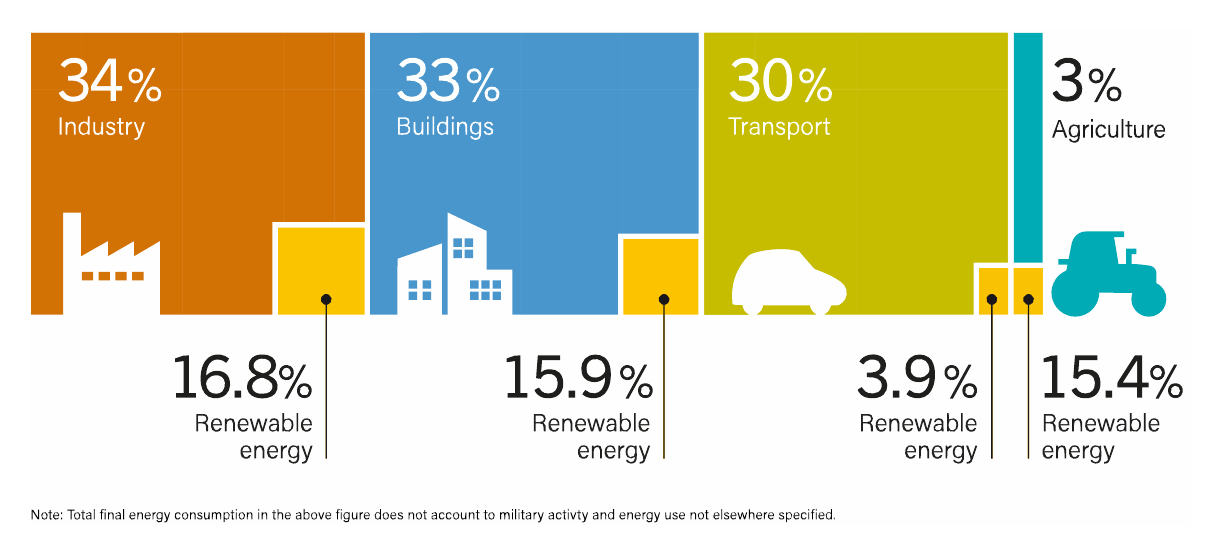
\begin{tikzpicture}[y=1cm, x=1cm, yscale=\globalscale,xscale=\globalscale, every node/.append style={scale=\globalscale}, inner sep=0pt, outer sep=0pt]
  \path[fill=cfefefe] (0.0, 78.9517).. controls (60.9441, 78.9517) and (121.8883, 78.9517) .. (184.6792, 78.9517).. controls (184.6792, 52.8976) and (184.6792, 26.8436) .. (184.6792, 0.0).. controls (123.735, 0.0) and (62.7909, 0.0) .. (0.0, 0.0).. controls (0.0, 26.054) and (0.0, 52.1081) .. (0.0, 78.9517) -- cycle;



  \path[fill=cd37204,shift={(0.5292, -0.8202)}] (0.0, 78.9517).. controls (17.48, 78.9517) and (34.9599, 78.9517) .. (52.9696, 78.9517).. controls (52.9696, 69.0504) and (52.9696, 59.1492) .. (52.9696, 48.9479).. controls (48.1325, 48.9479) and (43.2954, 48.9479) .. (38.3117, 48.9479).. controls (38.3117, 44.0933) and (38.3117, 39.2388) .. (38.3117, 34.2371).. controls (32.4268, 34.2371) and (26.5419, 34.2371) .. (20.4788, 34.2371).. controls (20.4788, 38.0876) and (20.4788, 41.938) .. (20.4788, 45.9052).. controls (20.1055, 45.6899) and (19.7327, 45.4748) .. (19.3621, 45.2551).. controls (19.1873, 45.1516) and (19.012, 45.0488) .. (18.8367, 44.9461).. controls (18.8205, 44.9366) and (18.8044, 44.9272) .. (18.7878, 44.9174).. controls (18.7053, 44.8691) and (18.6228, 44.8208) .. (18.5404, 44.7725).. controls (18.3954, 44.6876) and (18.2504, 44.6026) .. (18.1055, 44.5176).. controls (18.0579, 44.4897) and (18.0102, 44.4618) .. (17.9625, 44.4338).. controls (17.7993, 44.3382) and (17.6362, 44.2425) .. (17.473, 44.1468).. controls (17.1853, 43.9779) and (16.8976, 43.8091) .. (16.6092, 43.6414).. controls (16.5884, 43.6292) and (16.5676, 43.6171) .. (16.5462, 43.6045).. controls (16.4072, 43.524) and (16.4072, 43.524) .. (16.3777, 43.524).. controls (16.3777, 44.3098) and (16.3777, 45.0956) .. (16.3777, 45.9052).. controls (15.9156, 45.6449) and (15.9156, 45.6449) .. (15.4566, 45.3793).. controls (15.1496, 45.1995) and (14.8414, 45.0216) .. (14.5331, 44.844).. controls (14.3895, 44.7612) and (14.2459, 44.6784) .. (14.1023, 44.5955).. controls (13.9297, 44.4959) and (13.7571, 44.3964) .. (13.5845, 44.2969).. controls (13.5267, 44.2636) and (13.4689, 44.2303) .. (13.4111, 44.197).. controls (13.3829, 44.1808) and (13.3547, 44.1645) .. (13.3257, 44.1478).. controls (13.1814, 44.0646) and (13.0372, 43.9809) .. (12.8935, 43.8966).. controls (12.8649, 43.8799) and (12.8363, 43.8631) .. (12.8068, 43.8459).. controls (12.7527, 43.8142) and (12.6988, 43.7824) .. (12.6448, 43.7506).. controls (12.6204, 43.7363) and (12.596, 43.722) .. (12.5708, 43.7072).. controls (12.5391, 43.6885) and (12.5391, 43.6885) .. (12.5068, 43.6695).. controls (12.4141, 43.6179) and (12.3186, 43.5714) .. (12.2238, 43.524).. controls (12.2238, 44.3098) and (12.2238, 45.0956) .. (12.2238, 45.9052).. controls (11.7705, 45.6593) and (11.7705, 45.6593) .. (11.3242, 45.4025).. controls (11.0978, 45.2691) and (10.8693, 45.1409) .. (10.6381, 45.0161).. controls (10.4516, 44.9151) and (10.2673, 44.8108) .. (10.0834, 44.7051).. controls (9.9024, 44.6011) and (9.7205, 44.4988) .. (9.5382, 44.3971).. controls (9.0121, 44.103) and (9.0121, 44.103) .. (8.4917, 43.7991).. controls (8.4519, 43.7753) and (8.4519, 43.7753) .. (8.4112, 43.7511).. controls (8.36, 43.7205) and (8.3088, 43.6898) .. (8.2578, 43.6589).. controls (8.2347, 43.6451) and (8.2117, 43.6313) .. (8.1879, 43.6171).. controls (8.1575, 43.5987) and (8.1575, 43.5987) .. (8.1264, 43.58).. controls (8.0698, 43.5504) and (8.0698, 43.5504) .. (7.964, 43.524).. controls (7.964, 45.7941) and (7.964, 48.0642) .. (7.964, 50.4031).. controls (7.021, 50.4031) and (6.078, 50.4031) .. (5.1065, 50.4031).. controls (5.1065, 45.0683) and (5.1065, 39.7335) .. (5.1065, 34.2371).. controls (3.4213, 34.2371) and (1.7362, 34.2371) .. (0.0, 34.2371).. controls (0.0, 48.9929) and (0.0, 63.7487) .. (0.0, 78.9517) -- cycle;



  \path[fill=c4996cc,shift={(54.3454, -0.8202)}] (0.0, 78.9517).. controls (17.2093, 78.9517) and (34.4186, 78.9517) .. (52.1494, 78.9517).. controls (52.1494, 68.4305) and (52.1494, 57.9094) .. (52.1494, 47.0694).. controls (47.9234, 47.0694) and (43.6975, 47.0694) .. (39.3435, 47.0694).. controls (39.3435, 42.8347) and (39.3435, 38.6001) .. (39.3435, 34.2371).. controls (33.8167, 34.2371) and (28.2898, 34.2371) .. (22.5954, 34.2371).. controls (22.5954, 36.5945) and (22.5954, 38.952) .. (22.5954, 41.3808).. controls (21.2421, 41.3808) and (19.8887, 41.3808) .. (18.4944, 41.3808).. controls (18.4944, 43.4152) and (18.4944, 45.4496) .. (18.4944, 47.5456).. controls (18.442, 47.5631) and (18.3896, 47.5805) .. (18.3356, 47.5985).. controls (18.2733, 47.626) and (18.2118, 47.6541) .. (18.1503, 47.6833).. controls (18.1327, 47.6916) and (18.115, 47.6999) .. (18.0968, 47.7085).. controls (18.0391, 47.7357) and (17.9815, 47.763) .. (17.9239, 47.7904).. controls (17.8834, 47.8095) and (17.8429, 47.8286) .. (17.8024, 47.8478).. controls (17.5167, 47.9828) and (17.2322, 48.12) .. (16.9479, 48.2579).. controls (16.7032, 48.3764) and (16.4568, 48.4911) .. (16.2099, 48.6049).. controls (15.9604, 48.7203) and (15.7129, 48.8397) .. (15.4657, 48.9601).. controls (15.2251, 49.0771) and (14.9836, 49.1915) .. (14.7406, 49.3035).. controls (14.4502, 49.4372) and (14.1622, 49.5756) .. (13.8749, 49.7158).. controls (13.5879, 49.8557) and (13.2995, 49.9922) .. (13.0091, 50.125).. controls (12.7796, 50.2304) and (12.556, 50.3429) .. (12.3296, 50.456).. controls (12.3296, 45.1038) and (12.3296, 39.7515) .. (12.3296, 34.2371).. controls (12.0415, 34.2371) and (11.7533, 34.2371) .. (11.4565, 34.2371).. controls (11.4565, 37.9741) and (11.4565, 41.711) .. (11.4565, 45.5613).. controls (11.2818, 45.5001) and (11.1072, 45.439) .. (10.9273, 45.376).. controls (10.709, 45.3033) and (10.709, 45.3033) .. (10.6127, 45.2714).. controls (10.5334, 45.2448) and (10.4554, 45.216) .. (10.3775, 45.1859).. controls (10.26, 45.1429) and (10.1408, 45.1049) .. (10.0219, 45.066).. controls (9.9534, 45.0428) and (9.886, 45.0189) .. (9.8185, 44.9932).. controls (9.6843, 44.9423) and (9.5479, 44.8982) .. (9.4115, 44.8535).. controls (9.2978, 44.816) and (9.1854, 44.7762) .. (9.0735, 44.7336).. controls (8.9587, 44.6909) and (8.8418, 44.6543) .. (8.7255, 44.6162).. controls (8.6382, 44.5866) and (8.5522, 44.5553) .. (8.4661, 44.5226).. controls (8.3829, 44.4913) and (8.2991, 44.4614) .. (8.2153, 44.4318).. controls (8.1873, 44.4219) and (8.1873, 44.4219) .. (8.1587, 44.4118).. controls (7.9568, 44.3409) and (7.7538, 44.2736) .. (7.5505, 44.2067).. controls (7.4214, 44.164) and (7.2933, 44.1199) .. (7.1662, 44.0714).. controls (7.0522, 44.0288) and (6.936, 43.9926) .. (6.8205, 43.9547).. controls (6.752, 43.9315) and (6.6846, 43.9076) .. (6.6171, 43.882).. controls (6.4828, 43.8311) and (6.3465, 43.7869) .. (6.2101, 43.7422).. controls (6.0963, 43.7047) and (5.9839, 43.6649) .. (5.872, 43.6224).. controls (5.7572, 43.5797) and (5.6403, 43.5431) .. (5.524, 43.5049).. controls (5.4371, 43.4755) and (5.3514, 43.4442) .. (5.2657, 43.4117).. controls (5.1772, 43.3785) and (5.0881, 43.347) .. (4.999, 43.3156).. controls (4.9818, 43.3095) and (4.9646, 43.3034) .. (4.9469, 43.2971).. controls (4.754, 43.229) and (4.5599, 43.1654) .. (4.3656, 43.1006).. controls (4.3569, 40.1757) and (4.3482, 37.2507) .. (4.3392, 34.2371).. controls (2.9072, 34.2371) and (1.4753, 34.2371) .. (0.0, 34.2371).. controls (0.0, 48.9929) and (0.0, 63.7487) .. (0.0, 78.9517) -- cycle;



  \path[fill=cc6bd00,shift={(107.4208, -0.8202)}] (0.0, 78.9517).. controls (15.8996, 78.9517) and (31.7992, 78.9517) .. (48.1806, 78.9517).. controls (48.1806, 66.92) and (48.1806, 54.8883) .. (48.1806, 42.4921).. controls (46.382, 42.4921) and (44.5834, 42.4921) .. (42.7302, 42.4921).. controls (42.7302, 39.7679) and (42.7302, 37.0438) .. (42.7302, 34.2371).. controls (34.9157, 34.2371) and (27.1013, 34.2371) .. (19.05, 34.2371).. controls (19.1033, 34.2726) and (19.1572, 34.3071) .. (19.2116, 34.3407).. controls (19.6133, 34.5896) and (19.9108, 34.9167) .. (20.0257, 35.3911).. controls (20.0324, 35.4238) and (20.039, 35.4564) .. (20.0459, 35.49).. controls (20.0527, 35.5231) and (20.0596, 35.5561) .. (20.0666, 35.5901).. controls (20.0742, 35.6276) and (20.0742, 35.6276) .. (20.0819, 35.6658).. controls (20.0965, 35.6659) and (20.1112, 35.6659) .. (20.1263, 35.6659).. controls (20.28, 35.6665) and (20.4337, 35.6679) .. (20.5873, 35.6699).. controls (20.6446, 35.6705) and (20.7018, 35.6709) .. (20.759, 35.671).. controls (20.8416, 35.6713) and (20.9242, 35.6723) .. (21.0069, 35.6736).. controls (21.0321, 35.6735) and (21.0574, 35.6734) .. (21.0834, 35.6733).. controls (21.4334, 35.6807) and (21.661, 35.891) .. (21.9075, 36.1156).. controls (21.9208, 36.1274) and (21.9341, 36.1393) .. (21.9478, 36.1514).. controls (22.2719, 36.4414) and (22.5352, 36.8728) .. (22.5744, 37.3151).. controls (22.577, 37.3833) and (22.5777, 37.4513) .. (22.5772, 37.5196).. controls (22.577, 37.5571) and (22.577, 37.5571) .. (22.5768, 37.5954).. controls (22.5738, 37.7846) and (22.5599, 37.9716) .. (22.5375, 38.1595).. controls (22.5335, 38.1963) and (22.5335, 38.1963) .. (22.5295, 38.2338).. controls (22.4619, 38.7386) and (22.0375, 39.1379) .. (21.6521, 39.4381).. controls (21.2765, 39.7215) and (20.8721, 39.9623) .. (20.4582, 40.1849).. controls (20.4008, 40.2159) and (20.3437, 40.2474) .. (20.2866, 40.2789).. controls (19.6526, 40.625) and (18.981, 40.8966) .. (18.3093, 41.1596).. controls (18.2193, 41.1948) and (18.1295, 41.2305) .. (18.04, 41.2669).. controls (18.0221, 41.2742) and (18.0042, 41.2814) .. (17.9858, 41.2889).. controls (17.9368, 41.3088) and (17.8878, 41.3289) .. (17.8389, 41.3489).. controls (17.763, 41.3773) and (17.6905, 41.3975) .. (17.6113, 41.4139).. controls (17.4434, 41.4617) and (17.3552, 41.5922) .. (17.2508, 41.7248).. controls (17.2123, 41.7722) and (17.1737, 41.8196) .. (17.1351, 41.867).. controls (17.1155, 41.8912) and (17.0959, 41.9154) .. (17.0758, 41.9404).. controls (16.9968, 42.0348) and (16.9136, 42.1247) .. (16.8298, 42.2148).. controls (16.7297, 42.3229) and (16.6371, 42.436) .. (16.5447, 42.5508).. controls (16.4783, 42.6307) and (16.4088, 42.707) .. (16.338, 42.7831).. controls (16.2251, 42.9045) and (16.1195, 43.0301) .. (16.0156, 43.1593).. controls (15.9491, 43.2393) and (15.8797, 43.3156) .. (15.8089, 43.3917).. controls (15.6961, 43.5128) and (15.5908, 43.638) .. (15.4871, 43.767).. controls (15.4049, 43.8659) and (15.3181, 43.9601) .. (15.2302, 44.0539).. controls (15.1746, 44.1134) and (15.1266, 44.1703) .. (15.0813, 44.2383).. controls (15.0336, 44.2616) and (15.0336, 44.2616) .. (14.9767, 44.2762).. controls (14.9546, 44.2824) and (14.9326, 44.2886) .. (14.91, 44.295).. controls (14.8857, 44.3014) and (14.8615, 44.3078) .. (14.8365, 44.3144).. controls (14.8111, 44.3212) and (14.7857, 44.328) .. (14.7595, 44.335).. controls (14.2612, 44.4627) and (13.742, 44.541) .. (13.2292, 44.5823).. controls (13.1901, 44.5857) and (13.1901, 44.5857) .. (13.1502, 44.5893).. controls (12.8593, 44.6121) and (12.5691, 44.6128) .. (12.2775, 44.6122).. controls (12.1929, 44.6121) and (12.1084, 44.6122) .. (12.0238, 44.6124).. controls (11.4993, 44.6126) and (10.9834, 44.5867) .. (10.4626, 44.5244).. controls (10.4257, 44.52) and (10.4257, 44.52) .. (10.3881, 44.5156).. controls (9.652, 44.4272) and (8.9401, 44.2968) .. (8.2203, 44.1176).. controls (8.1905, 44.1102) and (8.1607, 44.1028) .. (8.13, 44.0952).. controls (7.9417, 44.0482) and (7.7541, 43.9992) .. (7.5671, 43.9473).. controls (7.5473, 43.9419) and (7.5275, 43.9365) .. (7.5072, 43.9309).. controls (7.2617, 43.8618) and (7.1086, 43.7606) .. (6.937, 43.5736).. controls (6.9155, 43.551) and (6.8939, 43.5284) .. (6.8717, 43.5052).. controls (6.7463, 43.3728) and (6.6244, 43.2383) .. (6.5126, 43.0943).. controls (6.4689, 43.0381) and (6.4244, 42.9835) .. (6.3784, 42.9292).. controls (6.0173, 42.5) and (5.7228, 42.0288) .. (5.4504, 41.5396).. controls (5.441, 41.5229) and (5.4315, 41.5062) .. (5.4217, 41.4891).. controls (4.9048, 40.5777) and (4.5627, 39.5101) .. (4.445, 38.4704).. controls (4.4414, 38.4406) and (4.4378, 38.4108) .. (4.4341, 38.38).. controls (4.3335, 37.5297) and (4.3613, 36.701) .. (4.445, 35.851).. controls (4.4978, 35.833) and (4.5507, 35.8155) .. (4.6038, 35.7981).. controls (4.6457, 35.7837) and (4.6457, 35.7837) .. (4.6885, 35.769).. controls (4.8179, 35.7384) and (4.9408, 35.7358) .. (5.0733, 35.7343).. controls (5.1, 35.7337) and (5.1268, 35.7332) .. (5.1543, 35.7327).. controls (5.2393, 35.7311) and (5.3242, 35.7299) .. (5.4091, 35.7287).. controls (5.4669, 35.7277) and (5.5247, 35.7266) .. (5.5824, 35.7256).. controls (5.7236, 35.723) and (5.8648, 35.7208) .. (6.006, 35.7188).. controls (6.0128, 35.6845) and (6.0196, 35.6502) .. (6.0266, 35.6149).. controls (6.0358, 35.5694) and (6.0451, 35.5239) .. (6.0543, 35.4784).. controls (6.0587, 35.4558) and (6.0632, 35.4333) .. (6.0677, 35.4101).. controls (6.1519, 34.9994) and (6.39, 34.6766) .. (6.7204, 34.4223).. controls (6.8151, 34.3641) and (6.9115, 34.312) .. (7.0115, 34.2635).. controls (7.0115, 34.2548) and (7.0115, 34.2461) .. (7.0115, 34.2371).. controls (4.6977, 34.2371) and (2.3839, 34.2371) .. (0.0, 34.2371).. controls (0.0, 48.9929) and (0.0, 63.7487) .. (0.0, 78.9517) -- cycle;



  \path[fill=cc6bd00,shift={(107.4208, -0.8467)}] (0.0, 78.9517).. controls (2.6456, 78.9517) and (5.2911, 78.9517) .. (8.0169, 78.9517).. controls (8.0169, 77.5023) and (8.0169, 76.0529) .. (8.0169, 74.5596).. controls (7.91, 74.6023) and (7.8127, 74.6488) .. (7.711, 74.7018).. controls (7.3395, 74.8903) and (6.9712, 74.9669) .. (6.5551, 74.9631).. controls (6.5262, 74.9629) and (6.4974, 74.9627) .. (6.4677, 74.9625).. controls (5.6653, 74.9518) and (5.0731, 74.6887) .. (4.5097, 74.1286).. controls (4.4432, 74.0549) and (4.392, 73.9819) .. (4.3392, 73.8981).. controls (4.3547, 73.8909) and (4.3702, 73.8837) .. (4.3862, 73.8762).. controls (4.4434, 73.8461) and (4.4887, 73.8134) .. (4.5384, 73.7724).. controls (4.5555, 73.7585) and (4.5726, 73.7446) .. (4.5902, 73.7303).. controls (4.6257, 73.7011) and (4.6612, 73.6719) .. (4.6967, 73.6426).. controls (4.7138, 73.6287) and (4.7308, 73.6148) .. (4.7484, 73.6005).. controls (4.7715, 73.5814) and (4.7715, 73.5814) .. (4.7951, 73.562).. controls (4.8438, 73.5263) and (4.893, 73.5003) .. (4.9477, 73.4748).. controls (4.9624, 73.4937) and (4.9772, 73.5125) .. (4.9924, 73.5319).. controls (5.2939, 73.9104) and (5.6438, 74.1807) .. (6.1383, 74.2421).. controls (6.5943, 74.2663) and (7.0334, 74.2499) .. (7.4118, 73.9609).. controls (7.6222, 73.7647) and (7.6981, 73.5471) .. (7.7098, 73.2641).. controls (7.7155, 72.9816) and (7.6503, 72.7717) .. (7.4613, 72.5537).. controls (7.2207, 72.3346) and (6.858, 72.2081) .. (6.5402, 72.1601).. controls (6.5071, 72.1551) and (6.5071, 72.1551) .. (6.4733, 72.1499).. controls (6.1601, 72.1076) and (5.8451, 72.1206) .. (5.5298, 72.1254).. controls (5.5298, 71.8897) and (5.5298, 71.6539) .. (5.5298, 71.411).. controls (5.5842, 71.4123) and (5.6385, 71.4135) .. (5.6945, 71.4148).. controls (6.3415, 71.4263) and (7.0641, 71.4352) .. (7.5671, 70.9613).. controls (7.7831, 70.7474) and (7.9144, 70.5042) .. (7.9211, 70.194).. controls (7.9202, 69.8258) and (7.8329, 69.4847) .. (7.5754, 69.21).. controls (7.1578, 68.8189) and (6.6256, 68.8031) .. (6.0854, 68.8181).. controls (5.7493, 68.8328) and (5.3985, 68.9775) .. (5.154, 69.2139).. controls (4.9953, 69.3943) and (4.859, 69.5909) .. (4.736, 69.7971).. controls (4.5425, 69.6947) and (4.356, 69.5847) .. (4.1712, 69.4674).. controls (4.101, 69.4267) and (4.101, 69.4267) .. (4.0481, 69.4267).. controls (4.3726, 68.8277) and (4.794, 68.3899) .. (5.4603, 68.1881).. controls (5.981, 68.0648) and (6.567, 68.051) .. (7.0908, 68.1567).. controls (7.1323, 68.1635) and (7.1323, 68.1635) .. (7.1745, 68.1704).. controls (7.494, 68.2306) and (7.7642, 68.3941) .. (8.0433, 68.5535).. controls (8.0433, 67.3399) and (8.0433, 66.1263) .. (8.0433, 64.8758).. controls (7.9473, 64.8671) and (7.8512, 64.8584) .. (7.7523, 64.8494).. controls (7.5469, 64.7756) and (7.3995, 64.6826) .. (7.3025, 64.479).. controls (7.2835, 64.3812) and (7.2835, 64.3812) .. (7.276, 64.2938).. controls (7.3634, 64.2938) and (7.4507, 64.2938) .. (7.5406, 64.2938).. controls (7.5428, 64.3172) and (7.545, 64.3407) .. (7.5472, 64.3649).. controls (7.5729, 64.4782) and (7.6199, 64.5493) .. (7.7173, 64.6145).. controls (7.804, 64.6473) and (7.8814, 64.6457) .. (7.9739, 64.646).. controls (8.0079, 64.6464) and (8.042, 64.6469) .. (8.077, 64.6473).. controls (8.2145, 64.6339) and (8.3007, 64.5938) .. (8.3956, 64.4938).. controls (8.4695, 64.3815) and (8.4698, 64.2879) .. (8.4683, 64.1548).. controls (8.4681, 64.1263) and (8.4678, 64.0978) .. (8.4676, 64.0684).. controls (8.4671, 64.0359) and (8.4671, 64.0359) .. (8.4667, 64.0027).. controls (8.4482, 64.0023) and (8.4296, 64.0019) .. (8.4106, 64.0015).. controls (8.3251, 63.9995) and (8.2396, 63.997) .. (8.1541, 63.9944).. controls (8.1105, 63.9935) and (8.1105, 63.9935) .. (8.0659, 63.9926).. controls (7.7947, 63.9838) and (7.5172, 63.9546) .. (7.3175, 63.7527).. controls (7.1795, 63.5975) and (7.1857, 63.4498) .. (7.1878, 63.2483).. controls (7.2003, 63.1182) and (7.2362, 63.0362) .. (7.329, 62.9444).. controls (7.454, 62.8476) and (7.5711, 62.7819) .. (7.7319, 62.783).. controls (7.7532, 62.7831) and (7.7744, 62.7832) .. (7.7963, 62.7833).. controls (7.8183, 62.7835) and (7.8404, 62.7837) .. (7.8631, 62.784).. controls (7.8966, 62.7842) and (7.8966, 62.7842) .. (7.9308, 62.7843).. controls (7.986, 62.7846) and (8.0411, 62.7851) .. (8.0963, 62.7856).. controls (8.0875, 62.7682) and (8.0788, 62.7507) .. (8.0698, 62.7327).. controls (8.0673, 62.6908) and (8.0665, 62.6487) .. (8.0665, 62.6067).. controls (8.0664, 62.5799) and (8.0664, 62.5531) .. (8.0663, 62.5254).. controls (8.0664, 62.4957) and (8.0665, 62.4659) .. (8.0665, 62.4353).. controls (8.0665, 62.388) and (8.0665, 62.388) .. (8.0664, 62.3398).. controls (8.0664, 62.2517) and (8.0664, 62.1636) .. (8.0666, 62.0754).. controls (8.0666, 61.9798) and (8.0666, 61.8842) .. (8.0665, 61.7886).. controls (8.0665, 61.6208) and (8.0665, 61.453) .. (8.0666, 61.2852).. controls (8.0668, 61.0356) and (8.0668, 60.7861) .. (8.0668, 60.5366).. controls (8.0667, 60.1169) and (8.0668, 59.6972) .. (8.067, 59.2775).. controls (8.0672, 58.8618) and (8.0673, 58.4461) .. (8.0673, 58.0304).. controls (8.0673, 58.0046) and (8.0673, 57.9787) .. (8.0673, 57.9521).. controls (8.0673, 57.821) and (8.0673, 57.6899) .. (8.0673, 57.5588).. controls (8.0674, 56.6294) and (8.0675, 55.7) .. (8.0678, 54.7705).. controls (8.068, 53.8675) and (8.0682, 52.9644) .. (8.0683, 52.0613).. controls (8.0683, 52.0335) and (8.0683, 52.0057) .. (8.0683, 51.977).. controls (8.0684, 51.6976) and (8.0684, 51.4182) .. (8.0685, 51.1388).. controls (8.0685, 50.5696) and (8.0686, 50.0004) .. (8.0687, 49.4312).. controls (8.0687, 49.4051) and (8.0687, 49.3789) .. (8.0687, 49.3519).. controls (8.0689, 47.6033) and (8.0693, 45.8547) .. (8.0698, 44.106).. controls (8.0416, 44.0985) and (8.0416, 44.0985) .. (8.0129, 44.0907).. controls (7.9265, 44.0674) and (7.8402, 44.0437) .. (7.7539, 44.0201).. controls (7.7096, 44.0081) and (7.7096, 44.0081) .. (7.6644, 43.996).. controls (7.3296, 43.9069) and (7.3296, 43.9069) .. (7.0511, 43.7107).. controls (7.0316, 43.6911) and (7.0121, 43.6714) .. (6.992, 43.6512).. controls (6.9624, 43.6201) and (6.9624, 43.6201) .. (6.9321, 43.5885).. controls (6.9007, 43.5563) and (6.9007, 43.5563) .. (6.8687, 43.5235).. controls (6.7438, 43.3943) and (6.6239, 43.2635) .. (6.5135, 43.1217).. controls (6.4694, 43.0652) and (6.4246, 43.0102) .. (6.3783, 42.9555).. controls (6.0173, 42.5264) and (5.7227, 42.0552) .. (5.4504, 41.566).. controls (5.441, 41.5494) and (5.4315, 41.5327) .. (5.4217, 41.5155).. controls (4.9048, 40.6042) and (4.5627, 39.5365) .. (4.445, 38.4969).. controls (4.4414, 38.467) and (4.4378, 38.4372) .. (4.4341, 38.4065).. controls (4.3335, 37.5562) and (4.3613, 36.7275) .. (4.445, 35.8775).. controls (4.4978, 35.8595) and (4.5507, 35.8419) .. (4.6038, 35.8246).. controls (4.6457, 35.8102) and (4.6457, 35.8102) .. (4.6885, 35.7955).. controls (4.8179, 35.7648) and (4.9408, 35.7623) .. (5.0733, 35.7607).. controls (5.1, 35.7602) and (5.1268, 35.7597) .. (5.1543, 35.7592).. controls (5.2393, 35.7576) and (5.3242, 35.7564) .. (5.4091, 35.7551).. controls (5.4669, 35.7541) and (5.5247, 35.7531) .. (5.5824, 35.752).. controls (5.7236, 35.7495) and (5.8648, 35.7472) .. (6.006, 35.7452).. controls (6.0128, 35.711) and (6.0196, 35.6767) .. (6.0266, 35.6414).. controls (6.0358, 35.5959) and (6.0451, 35.5503) .. (6.0543, 35.5048).. controls (6.0587, 35.4823) and (6.0632, 35.4598) .. (6.0677, 35.4366).. controls (6.1519, 35.0258) and (6.39, 34.703) .. (6.7204, 34.4487).. controls (6.8151, 34.3905) and (6.9115, 34.3385) .. (7.0115, 34.29).. controls (7.0115, 34.2813) and (7.0115, 34.2725) .. (7.0115, 34.2635).. controls (4.6977, 34.2635) and (2.3839, 34.2635) .. (0.0, 34.2635).. controls (0.0, 49.0106) and (0.0, 63.7577) .. (0.0, 78.9517) -- cycle;



  \path[fill=cc6bd00,shift={(131.5244, -0.8467)}] (0.0, 78.9517).. controls (7.9367, 78.9517) and (15.8734, 78.9517) .. (24.0506, 78.9517).. controls (24.0506, 76.0092) and (24.0506, 73.0668) .. (24.0506, 70.0352).. controls (16.1139, 70.0352) and (8.1772, 70.0352) .. (0.0, 70.0352).. controls (0.0, 72.9776) and (0.0, 75.9201) .. (0.0, 78.9517) -- cycle;



  \path[fill=cfbc400,shift={(39.7404, -31.7235)}] (0.0, 78.9517).. controls (4.5402, 78.9517) and (9.0805, 78.9517) .. (13.7583, 78.9517).. controls (13.7583, 74.394) and (13.7583, 69.8362) .. (13.7583, 65.1404).. controls (11.7763, 65.1404) and (9.7943, 65.1404) .. (7.7523, 65.1404).. controls (7.7523, 57.5879) and (7.7523, 50.0354) .. (7.7523, 42.254).. controls (7.6824, 42.254) and (7.6126, 42.254) .. (7.5406, 42.254).. controls (7.5406, 49.8065) and (7.5406, 57.359) .. (7.5406, 65.1404).. controls (5.0522, 65.1404) and (2.5638, 65.1404) .. (0.0, 65.1404).. controls (0.0, 69.6981) and (0.0, 74.2558) .. (0.0, 78.9517) -- cycle;



  \path[fill=c01abb5,shift={(156.554, -0.8202)}] (0.0, 78.9517).. controls (1.5105, 78.9517) and (3.021, 78.9517) .. (4.5773, 78.9517).. controls (4.5773, 66.92) and (4.5773, 54.8883) .. (4.5773, 42.4921).. controls (3.0668, 42.4921) and (1.5563, 42.4921) .. (0.0, 42.4921).. controls (0.0, 54.5237) and (0.0, 66.5554) .. (0.0, 78.9517) -- cycle;



  \path[fill=c00abb5,shift={(168.4645, -32.3231)}] (0.0, 78.9517).. controls (0.0613, 78.9516) and (0.1226, 78.9517) .. (0.1839, 78.9517).. controls (0.3494, 78.9517) and (0.5148, 78.9513) .. (0.6803, 78.9507).. controls (0.8536, 78.9502) and (1.0268, 78.9502) .. (1.2001, 78.9501).. controls (1.4906, 78.9499) and (1.7811, 78.9494) .. (2.0716, 78.9486).. controls (2.3707, 78.9479) and (2.6697, 78.9474) .. (2.9687, 78.947).. controls (2.9872, 78.947) and (3.0057, 78.947) .. (3.0247, 78.947).. controls (3.1174, 78.9468) and (3.2101, 78.9467) .. (3.3028, 78.9467).. controls (4.0702, 78.9458) and (4.8375, 78.9444) .. (5.6049, 78.9427).. controls (5.6049, 78.6458) and (5.6049, 78.3489) .. (5.6049, 78.0431).. controls (5.0636, 78.0431) and (4.5222, 78.0431) .. (3.9645, 78.0431).. controls (3.9819, 77.9732) and (3.9994, 77.9034) .. (4.0174, 77.8314).. controls (4.0286, 77.7731) and (4.0391, 77.7146) .. (4.0489, 77.656).. controls (4.0573, 77.6057) and (4.0573, 77.6057) .. (4.066, 77.5544).. controls (4.072, 77.5178) and (4.0781, 77.4813) .. (4.0841, 77.4447).. controls (4.0906, 77.4058) and (4.0972, 77.3668) .. (4.1037, 77.3279).. controls (4.1213, 77.2226) and (4.1388, 77.1173) .. (4.1563, 77.012).. controls (4.1747, 76.9017) and (4.1931, 76.7914) .. (4.2115, 76.681).. controls (4.2424, 76.4959) and (4.2732, 76.3108) .. (4.304, 76.1256).. controls (4.3396, 75.9116) and (4.3753, 75.6976) .. (4.411, 75.4836).. controls (4.4418, 75.2996) and (4.4724, 75.1157) .. (4.503, 74.9317).. controls (4.5213, 74.8219) and (4.5396, 74.7121) .. (4.558, 74.6024).. controls (4.5752, 74.4993) and (4.5924, 74.3962) .. (4.6094, 74.293).. controls (4.6157, 74.2552) and (4.622, 74.2173) .. (4.6284, 74.1795).. controls (4.637, 74.1279) and (4.6456, 74.0763) .. (4.6541, 74.0246).. controls (4.6589, 73.9957) and (4.6637, 73.9668) .. (4.6687, 73.9371).. controls (4.6788, 73.8627) and (4.6788, 73.8627) .. (4.6788, 73.7568).. controls (5.0805, 73.7568) and (5.4821, 73.7568) .. (5.8959, 73.7568).. controls (5.8959, 74.5601) and (5.8959, 75.3634) .. (5.8959, 76.191).. controls (6.4373, 76.191) and (6.9786, 76.191) .. (7.5363, 76.191).. controls (7.5363, 75.9029) and (7.5363, 75.6147) .. (7.5363, 75.3179).. controls (7.2919, 75.3179) and (7.0474, 75.3179) .. (6.7955, 75.3179).. controls (6.7955, 74.794) and (6.7955, 74.2701) .. (6.7955, 73.7304).. controls (7.0487, 73.7304) and (7.3019, 73.7304) .. (7.5628, 73.7304).. controls (7.7396, 73.7186) and (7.9145, 73.7051) .. (8.0903, 73.6857).. controls (8.1359, 73.681) and (8.1815, 73.6762) .. (8.2271, 73.6715).. controls (8.5513, 73.6374) and (8.8749, 73.5983) .. (9.1983, 73.5567).. controls (9.2191, 73.5541) and (9.2399, 73.5515) .. (9.2614, 73.5487).. controls (9.9414, 73.4618) and (9.9414, 73.4618) .. (10.2351, 73.2541).. controls (10.2519, 73.2424) and (10.2688, 73.2308) .. (10.2862, 73.2188).. controls (10.5286, 73.0324) and (10.6706, 72.7316) .. (10.7113, 72.4339).. controls (10.7136, 72.3745) and (10.7145, 72.315) .. (10.7144, 72.2556).. controls (10.7144, 72.2385) and (10.7144, 72.2215) .. (10.7144, 72.2039).. controls (10.7143, 72.1481) and (10.7141, 72.0922) .. (10.7139, 72.0364).. controls (10.7139, 71.9975) and (10.7138, 71.9586) .. (10.7138, 71.9196).. controls (10.7137, 71.8176) and (10.7135, 71.7156) .. (10.7132, 71.6135).. controls (10.7129, 71.5092) and (10.7128, 71.4049) .. (10.7126, 71.3006).. controls (10.7124, 71.0963) and (10.7119, 70.892) .. (10.7113, 70.6877).. controls (10.736, 70.6798) and (10.7606, 70.672) .. (10.786, 70.6639).. controls (11.0443, 70.5744) and (11.2579, 70.371) .. (11.4522, 70.1849).. controls (11.4704, 70.1684) and (11.4885, 70.1519) .. (11.5073, 70.1349).. controls (11.8247, 69.8369) and (12.0863, 69.3919) .. (12.193, 68.9679).. controls (12.204, 68.93) and (12.204, 68.93) .. (12.2151, 68.8914).. controls (12.2729, 68.6592) and (12.28, 68.4341) .. (12.2807, 68.1956).. controls (12.2808, 68.1645) and (12.2809, 68.1334) .. (12.2811, 68.1014).. controls (12.2787, 67.809) and (12.2411, 67.5383) .. (12.1368, 67.2646).. controls (12.1287, 67.2432) and (12.1207, 67.2218) .. (12.1123, 67.1997).. controls (11.9921, 66.8909) and (11.8262, 66.6273) .. (11.6109, 66.3749).. controls (11.5907, 66.3482) and (11.5706, 66.3215) .. (11.5497, 66.2939).. controls (11.2592, 65.9763) and (10.8683, 65.7438) .. (10.4732, 65.5812).. controls (10.4539, 65.5731) and (10.4345, 65.565) .. (10.4146, 65.5567).. controls (9.7667, 65.3142) and (9.0198, 65.3742) .. (8.3929, 65.644).. controls (7.7064, 65.9575) and (7.1678, 66.5158) .. (6.9013, 67.2216).. controls (6.6773, 67.8897) and (6.7084, 68.5041) .. (6.9013, 69.1795).. controls (5.1551, 69.1883) and (3.4088, 69.197) .. (1.6097, 69.206).. controls (1.6097, 69.0663) and (1.6097, 68.9266) .. (1.6097, 68.7827).. controls (1.5951, 68.6532) and (1.5951, 68.6532) .. (1.575, 68.5495).. controls (1.5695, 68.5213) and (1.5695, 68.5213) .. (1.5639, 68.4926).. controls (1.4149, 67.7435) and (1.0746, 67.1146) .. (0.5513, 66.5602).. controls (0.5335, 66.5406) and (0.5157, 66.5211) .. (0.4974, 66.501).. controls (0.2285, 66.217) and (-0.1071, 65.9964) .. (-0.4541, 65.8193).. controls (-0.4698, 65.8113) and (-0.4854, 65.8032) .. (-0.5016, 65.795).. controls (-0.8142, 65.6385) and (-1.1458, 65.5511) .. (-1.4859, 65.4754).. controls (-1.5093, 65.4701) and (-1.5327, 65.4649) .. (-1.5568, 65.4596).. controls (-2.3862, 65.2909) and (-3.2706, 65.4903) .. (-3.9995, 65.8987).. controls (-4.017, 65.9085) and (-4.0345, 65.9183) .. (-4.0526, 65.9284).. controls (-4.925, 66.4263) and (-5.5325, 67.2445) .. (-5.801, 68.2065).. controls (-5.8287, 68.3099) and (-5.8539, 68.4138) .. (-5.878, 68.5181).. controls (-5.8846, 68.5458) and (-5.8912, 68.5736) .. (-5.898, 68.6022).. controls (-6.0825, 69.5545) and (-5.8079, 70.5535) .. (-5.2745, 71.345).. controls (-4.8546, 71.9498) and (-4.2947, 72.3913) .. (-3.6291, 72.6985).. controls (-3.6116, 72.6985) and (-3.5941, 72.6985) .. (-3.5762, 72.6985).. controls (-3.5727, 72.7247) and (-3.5727, 72.7247) .. (-3.5692, 72.7514).. controls (-3.5247, 73.0648) and (-3.456, 73.3649) .. (-3.3909, 73.6774).. controls (-3.8712, 73.6774) and (-4.3514, 73.6774) .. (-4.8462, 73.6774).. controls (-4.8462, 73.9656) and (-4.8462, 74.2537) .. (-4.8462, 74.5506).. controls (-4.3048, 74.5506) and (-3.7635, 74.5506) .. (-3.2057, 74.5506).. controls (-3.1926, 74.6553) and (-3.1926, 74.6553) .. (-3.1793, 74.7622).. controls (-3.1683, 74.8227) and (-3.1567, 74.8831) .. (-3.1444, 74.9434).. controls (-3.141, 74.9601) and (-3.1376, 74.9769) .. (-3.1341, 74.9942).. controls (-3.1229, 75.0491) and (-3.1116, 75.1041) .. (-3.1003, 75.159).. controls (-3.0924, 75.1981) and (-3.0844, 75.2371) .. (-3.0765, 75.2761).. controls (-3.0555, 75.3789) and (-3.0345, 75.4817) .. (-3.0135, 75.5845).. controls (-2.9884, 75.7069) and (-2.9635, 75.8292) .. (-2.9385, 75.9516).. controls (-2.9183, 76.0511) and (-2.898, 76.1505) .. (-2.8776, 76.25).. controls (-2.841, 76.4291) and (-2.8047, 76.6083) .. (-2.7696, 76.7878).. controls (-2.7637, 76.8181) and (-2.7577, 76.8485) .. (-2.7516, 76.8798).. controls (-2.7408, 76.9352) and (-2.7301, 76.9906) .. (-2.7195, 77.046).. controls (-2.683, 77.2327) and (-2.6332, 77.3976) .. (-2.5443, 77.5668).. controls (-2.5323, 77.5912) and (-2.5204, 77.6157) .. (-2.5081, 77.6408).. controls (-2.2353, 78.1746) and (-1.749, 78.6001) .. (-1.1858, 78.8066).. controls (-1.1188, 78.828) and (-1.0513, 78.8456) .. (-0.9832, 78.8633).. controls (-0.9471, 78.8735) and (-0.9471, 78.8735) .. (-0.9102, 78.8839).. controls (-0.608, 78.96) and (-0.3098, 78.9533) .. (0.0, 78.9517) -- cycle;



  \path[fill=cfbc300,shift={(94.5621, -33.5756)}] (0.0, 78.9517).. controls (3.9291, 78.9517) and (7.8581, 78.9517) .. (11.9063, 78.9517).. controls (11.9063, 75.0051) and (11.9063, 71.0586) .. (11.9063, 66.9925).. controls (10.1425, 66.9925) and (8.3788, 66.9925) .. (6.5617, 66.9925).. controls (6.5617, 59.44) and (6.5617, 51.8874) .. (6.5617, 44.106).. controls (6.4831, 44.106) and (6.4045, 44.106) .. (6.3235, 44.106).. controls (6.3235, 51.6586) and (6.3235, 59.2111) .. (6.3235, 66.9925).. controls (4.2368, 66.9925) and (2.15, 66.9925) .. (0.0, 66.9925).. controls (0.0, 70.939) and (0.0, 74.8855) .. (0.0, 78.9517) -- cycle;



  \path[fill=c4996cc,shift={(78.449, -0.8467)}] (0.0, 78.9517).. controls (5.2911, 78.9517) and (10.5823, 78.9517) .. (16.0338, 78.9517).. controls (16.0338, 76.0092) and (16.0338, 73.0668) .. (16.0338, 70.0352).. controls (10.7426, 70.0352) and (5.4515, 70.0352) .. (0.0, 70.0352).. controls (0.0, 72.9776) and (0.0, 75.9201) .. (0.0, 78.9517) -- cycle;



  \path[fill=cd37204,shift={(24.6327, -0.8467)}] (0.0, 78.9517).. controls (5.2911, 78.9517) and (10.5823, 78.9517) .. (16.0338, 78.9517).. controls (16.0338, 76.0092) and (16.0338, 73.0668) .. (16.0338, 70.0352).. controls (10.7426, 70.0352) and (5.4515, 70.0352) .. (0.0, 70.0352).. controls (0.0, 72.9776) and (0.0, 75.9201) .. (0.0, 78.9517) -- cycle;



  \path[fill=c4996cc,shift={(62.3888, -0.8467)}] (0.0, 78.9517).. controls (5.2911, 78.9517) and (10.5823, 78.9517) .. (16.0338, 78.9517).. controls (16.0338, 76.0092) and (16.0338, 73.0668) .. (16.0338, 70.0352).. controls (12.2238, 70.0352) and (12.2238, 70.0352) .. (11.9856, 70.2469).. controls (11.6677, 70.4299) and (11.291, 70.4681) .. (10.9337, 70.3815).. controls (10.7494, 70.3083) and (10.5713, 70.2034) .. (10.4503, 70.0438).. controls (10.3316, 69.951) and (10.2232, 69.9699) .. (10.0773, 69.9773).. controls (10.0249, 69.9794) and (9.9725, 69.9812) .. (9.92, 69.9828).. controls (9.8969, 69.9839) and (9.8738, 69.985) .. (9.8499, 69.9862).. controls (9.7821, 69.9869) and (9.7821, 69.9869) .. (9.7102, 69.9294).. controls (9.7484, 70.0302) and (9.7941, 70.1239) .. (9.8449, 70.219).. controls (9.8611, 70.2494) and (9.8774, 70.2798) .. (9.8941, 70.3112).. controls (9.9116, 70.3438) and (9.9292, 70.3764) .. (9.9467, 70.4089).. controls (9.9555, 70.4254) and (9.9644, 70.4419) .. (9.9735, 70.4589).. controls (10.097, 70.6892) and (10.2242, 70.9167) .. (10.3566, 71.1419).. controls (10.4173, 71.2455) and (10.4747, 71.3492) .. (10.5271, 71.4573).. controls (10.6006, 71.6089) and (10.6834, 71.7543) .. (10.7669, 71.9005).. controls (10.9013, 72.1362) and (11.0313, 72.3738) .. (11.1588, 72.6132).. controls (11.2987, 72.876) and (11.4408, 73.1371) .. (11.5888, 73.3954).. controls (11.4341, 73.4251) and (11.2834, 73.4435) .. (11.139, 73.369).. controls (10.9969, 73.2127) and (10.9178, 73.0057) .. (10.8322, 72.815).. controls (10.783, 72.7079) and (10.7264, 72.6062) .. (10.6677, 72.5041).. controls (10.6464, 72.4661) and (10.6252, 72.428) .. (10.604, 72.3899).. controls (10.5926, 72.3694) and (10.5812, 72.3489) .. (10.5694, 72.3278).. controls (10.4872, 72.18) and (10.4054, 72.032) .. (10.3237, 71.884).. controls (10.3101, 71.8593) and (10.3101, 71.8593) .. (10.2962, 71.8341).. controls (10.1715, 71.6082) and (10.0478, 71.3818) .. (9.9252, 71.1547).. controls (9.4258, 70.2304) and (9.4258, 70.2304) .. (9.2604, 69.9823).. controls (9.2047, 69.9729) and (9.2047, 69.9729) .. (9.1345, 69.9738).. controls (9.0947, 69.9739) and (9.0947, 69.9739) .. (9.054, 69.9741).. controls (9.0248, 69.9746) and (8.9955, 69.9752) .. (8.9654, 69.9757).. controls (8.9193, 69.9761) and (8.9193, 69.9761) .. (8.8723, 69.9765).. controls (8.7704, 69.9774) and (8.6684, 69.9788) .. (8.5665, 69.9803).. controls (8.496, 69.9811) and (8.4255, 69.9818) .. (8.355, 69.9824).. controls (8.1881, 69.9841) and (8.0212, 69.9862) .. (7.8543, 69.9884).. controls (7.6643, 69.9908) and (7.4744, 69.9929) .. (7.2844, 69.9949).. controls (6.8935, 69.999) and (6.5027, 70.0037) .. (6.1119, 70.0088).. controls (6.1071, 70.0598) and (6.1071, 70.0598) .. (6.1022, 70.1119).. controls (6.0978, 70.1572) and (6.0933, 70.2026) .. (6.0888, 70.2479).. controls (6.0868, 70.2703) and (6.0847, 70.2926) .. (6.0826, 70.3156).. controls (6.04, 70.7402) and (5.8473, 71.1174) .. (5.5147, 71.3907).. controls (5.3014, 71.546) and (5.0844, 71.6475) .. (4.835, 71.7274).. controls (4.7625, 71.755) and (4.7625, 71.755) .. (4.736, 71.8079).. controls (4.7497, 71.8139) and (4.7635, 71.8198) .. (4.7776, 71.826).. controls (5.2392, 72.0293) and (5.5918, 72.2432) .. (5.799, 72.726).. controls (5.8657, 72.9121) and (5.8831, 73.0687) .. (5.882, 73.2664).. controls (5.8818, 73.307) and (5.8818, 73.307) .. (5.8816, 73.3485).. controls (5.8742, 73.8106) and (5.7322, 74.1544) .. (5.3975, 74.4802).. controls (5.1788, 74.6802) and (4.9303, 74.7811) .. (4.6517, 74.8705).. controls (4.6344, 74.876) and (4.6172, 74.8816) .. (4.5994, 74.8874).. controls (4.3576, 74.9616) and (4.119, 74.9613) .. (3.8679, 74.9614).. controls (3.8359, 74.9617) and (3.804, 74.9621) .. (3.7711, 74.9624).. controls (3.5748, 74.9627) and (3.393, 74.9457) .. (3.2015, 74.9035).. controls (3.1744, 74.8986) and (3.1473, 74.8936) .. (3.1194, 74.8885).. controls (2.5832, 74.7706) and (2.0446, 74.4279) .. (1.7372, 73.9679).. controls (1.7227, 73.9449) and (1.7082, 73.9218) .. (1.6933, 73.8981).. controls (1.7166, 73.8873) and (1.7166, 73.8873) .. (1.7404, 73.8762).. controls (1.7976, 73.8461) and (1.8428, 73.8134) .. (1.8926, 73.7724).. controls (1.9097, 73.7585) and (1.9268, 73.7446) .. (1.9444, 73.7303).. controls (1.9799, 73.7011) and (2.0153, 73.6719) .. (2.0508, 73.6426).. controls (2.0679, 73.6287) and (2.085, 73.6148) .. (2.1026, 73.6005).. controls (2.118, 73.5878) and (2.1334, 73.5751) .. (2.1493, 73.562).. controls (2.198, 73.5263) and (2.2472, 73.5003) .. (2.3019, 73.4748).. controls (2.3166, 73.4937) and (2.3313, 73.5125) .. (2.3465, 73.5319).. controls (2.6492, 73.9118) and (2.9965, 74.1807) .. (3.4925, 74.2421).. controls (3.9446, 74.2771) and (4.3922, 74.2463) .. (4.766, 73.9609).. controls (4.9686, 73.7719) and (5.0535, 73.5554) .. (5.064, 73.2835).. controls (5.0694, 72.9932) and (5.0114, 72.7804) .. (4.8171, 72.5554).. controls (4.5806, 72.3424) and (4.2779, 72.2287) .. (3.9688, 72.1783).. controls (3.9298, 72.1703) and (3.9298, 72.1703) .. (3.8901, 72.1621).. controls (3.5587, 72.1017) and (3.2192, 72.1221) .. (2.884, 72.1254).. controls (2.884, 71.8897) and (2.884, 71.6539) .. (2.884, 71.411).. controls (2.9411, 71.4117) and (2.9982, 71.4123) .. (3.0571, 71.4129).. controls (3.1136, 71.4133) and (3.1702, 71.4136) .. (3.2268, 71.4139).. controls (3.2655, 71.4142) and (3.3042, 71.4146) .. (3.3429, 71.415).. controls (3.8931, 71.4215) and (4.5007, 71.351) .. (4.9213, 70.9613).. controls (5.1588, 70.7265) and (5.2574, 70.486) .. (5.2683, 70.1518).. controls (5.2685, 70.0688) and (5.2676, 69.9859) .. (5.2652, 69.9029).. controls (5.2565, 69.9378) and (5.2477, 69.9728) .. (5.2388, 70.0088).. controls (3.8417, 70.0088) and (2.4448, 70.0088) .. (1.0054, 70.0088).. controls (0.988, 70.1746) and (0.9705, 70.3405) .. (0.9525, 70.5115).. controls (0.818, 70.9924) and (0.5496, 71.334) .. (0.1133, 71.5803).. controls (-0.0115, 71.6412) and (-0.1394, 71.6851) .. (-0.2715, 71.7274).. controls (-0.344, 71.755) and (-0.344, 71.755) .. (-0.3704, 71.8079).. controls (-0.3567, 71.8139) and (-0.343, 71.8198) .. (-0.3289, 71.826).. controls (0.1327, 72.0293) and (0.4854, 72.2432) .. (0.6926, 72.726).. controls (0.7592, 72.9121) and (0.7767, 73.0687) .. (0.7756, 73.2664).. controls (0.7754, 73.2935) and (0.7753, 73.3206) .. (0.7751, 73.3485).. controls (0.7683, 73.7765) and (0.6514, 74.1034) .. (0.3541, 74.4193).. controls (0.2477, 74.5221) and (0.1331, 74.6253) .. (0.0, 74.6919).. controls (0.0, 76.0976) and (0.0, 77.5033) .. (0.0, 78.9517) -- cycle;



  \path[fill=cc6bd00,shift={(115.4642, -0.8467)}] (0.0, 78.9517).. controls (5.2911, 78.9517) and (10.5823, 78.9517) .. (16.0338, 78.9517).. controls (16.0338, 76.0092) and (16.0338, 73.0668) .. (16.0338, 70.0352).. controls (11.9327, 70.0352) and (11.9327, 70.0352) .. (11.6946, 70.2469).. controls (11.3791, 70.4285) and (11.0115, 70.4621) .. (10.6554, 70.3874).. controls (10.5912, 70.3631) and (10.5359, 70.3357) .. (10.4775, 70.2998).. controls (10.4459, 70.2811) and (10.4459, 70.2811) .. (10.4137, 70.2621).. controls (10.3228, 70.2048) and (10.2515, 70.1573) .. (10.1867, 70.0703).. controls (10.0613, 69.9733) and (9.9349, 69.9946) .. (9.7813, 70.0005).. controls (9.7516, 70.0011) and (9.7219, 70.0017) .. (9.6913, 70.0023).. controls (9.6182, 70.0038) and (9.5452, 70.006) .. (9.4721, 70.0088).. controls (9.5071, 70.1238) and (9.552, 70.2237) .. (9.6107, 70.3285).. controls (9.6191, 70.3436) and (9.6274, 70.3587) .. (9.6361, 70.3742).. controls (9.6634, 70.4233) and (9.691, 70.4724) .. (9.7185, 70.5214).. controls (9.7572, 70.5908) and (9.7958, 70.6603) .. (9.8344, 70.7297).. controls (9.8441, 70.7471) and (9.8538, 70.7646) .. (9.8638, 70.7825).. controls (9.9524, 70.9416) and (10.039, 71.1018) .. (10.1253, 71.2622).. controls (10.2348, 71.4654) and (10.3467, 71.6669) .. (10.461, 71.8674).. controls (10.6085, 72.1265) and (10.7499, 72.3885) .. (10.89, 72.6516).. controls (11.0231, 72.9012) and (11.1591, 73.1489) .. (11.2977, 73.3954).. controls (11.1398, 73.4355) and (10.994, 73.4532) .. (10.8479, 73.369).. controls (10.6824, 73.1774) and (10.5811, 72.9313) .. (10.4737, 72.7039).. controls (10.4042, 72.5576) and (10.3258, 72.4161) .. (10.2476, 72.2742).. controls (10.2196, 72.2224) and (10.1916, 72.1705) .. (10.1636, 72.1186).. controls (10.0679, 71.9425) and (9.9686, 71.7685) .. (9.8694, 71.5944).. controls (9.7551, 71.3928) and (9.6454, 71.189) .. (9.5366, 70.9844).. controls (9.1386, 70.2361) and (9.1386, 70.2361) .. (8.9694, 69.9823).. controls (8.912, 69.9729) and (8.912, 69.9729) .. (8.8395, 69.9738).. controls (8.812, 69.9739) and (8.7846, 69.974) .. (8.7563, 69.9741).. controls (8.726, 69.9746) and (8.6958, 69.9752) .. (8.6646, 69.9757).. controls (8.6329, 69.976) and (8.6011, 69.9762) .. (8.5684, 69.9765).. controls (8.4812, 69.9772) and (8.394, 69.9783) .. (8.3069, 69.9796).. controls (8.2158, 69.9808) and (8.1247, 69.9816) .. (8.0336, 69.9824).. controls (7.8611, 69.9841) and (7.6886, 69.9862) .. (7.5161, 69.9884).. controls (7.3198, 69.9908) and (7.1234, 69.9929) .. (6.927, 69.9949).. controls (6.523, 69.999) and (6.119, 70.0037) .. (5.715, 70.0088).. controls (5.7181, 70.0265) and (5.7211, 70.0442) .. (5.7243, 70.0624).. controls (5.7384, 70.1443) and (5.7523, 70.2262) .. (5.7663, 70.3081).. controls (5.7711, 70.3359) and (5.7759, 70.3638) .. (5.7809, 70.3924).. controls (5.8242, 70.6481) and (5.851, 70.9017) .. (5.8527, 71.161).. controls (5.8529, 71.1915) and (5.8529, 71.1915) .. (5.8532, 71.2227).. controls (5.8595, 72.1112) and (5.8307, 73.009) .. (5.424, 73.8187).. controls (5.4048, 73.8584) and (5.4048, 73.8584) .. (5.3853, 73.899).. controls (5.132, 74.3971) and (4.7246, 74.716) .. (4.2069, 74.9035).. controls (3.6638, 75.0441) and (3.0752, 74.9712) .. (2.5896, 74.6985).. controls (2.0593, 74.3654) and (1.7503, 73.8006) .. (1.5875, 73.2102).. controls (1.5781, 73.1783) and (1.5687, 73.1464) .. (1.559, 73.1136).. controls (1.2856, 72.1282) and (1.3567, 71.0031) .. (1.5346, 70.0088).. controls (1.2639, 70.0088) and (0.9932, 70.0088) .. (0.7144, 70.0088).. controls (0.7084, 70.0841) and (0.7024, 70.1594) .. (0.6962, 70.237).. controls (0.6643, 70.566) and (0.5782, 70.8566) .. (0.3704, 71.12).. controls (0.3559, 71.1395) and (0.3413, 71.1589) .. (0.3263, 71.179).. controls (0.0847, 71.4783) and (-0.2979, 71.6734) .. (-0.6615, 71.7815).. controls (-0.6035, 71.8394) and (-0.5674, 71.8521) .. (-0.4911, 71.879).. controls (-0.1017, 72.0304) and (0.2032, 72.2918) .. (0.3787, 72.6728).. controls (0.5375, 73.043) and (0.5388, 73.5487) .. (0.3969, 73.9246).. controls (0.2933, 74.1622) and (0.1897, 74.2905) .. (0.0, 74.4802).. controls (0.0, 75.9558) and (0.0, 77.4314) .. (0.0, 78.9517) -- cycle;



  \path[fill=c4996cc,shift={(94.5092, -0.8467)}] (0.0, 78.9517).. controls (3.9465, 78.9517) and (7.8931, 78.9517) .. (11.9592, 78.9517).. controls (11.9592, 76.0092) and (11.9592, 73.0668) .. (11.9592, 70.0352).. controls (8.0126, 70.0352) and (4.0661, 70.0352) .. (0.0, 70.0352).. controls (0.0, 72.9776) and (0.0, 75.9201) .. (0.0, 78.9517) -- cycle;



  \path[fill=cd37204,shift={(48.7098, -9.7896)}] (0.0, 78.9517).. controls (1.5804, 78.9517) and (3.1607, 78.9517) .. (4.789, 78.9517).. controls (4.789, 72.0103) and (4.789, 65.069) .. (4.789, 57.9173).. controls (3.2086, 57.9173) and (1.6282, 57.9173) .. (0.0, 57.9173).. controls (0.0, 64.8586) and (0.0, 71.8) .. (0.0, 78.9517) -- cycle;



  \path[fill=cd37204,shift={(40.6929, -0.8467)}] (0.0, 78.9517).. controls (2.6368, 78.9517) and (5.2737, 78.9517) .. (7.9904, 78.9517).. controls (7.9904, 76.0092) and (7.9904, 73.0668) .. (7.9904, 70.0352).. controls (5.3536, 70.0352) and (2.7167, 70.0352) .. (0.0, 70.0352).. controls (0.0, 72.9776) and (0.0, 75.9201) .. (0.0, 78.9517) -- cycle;



  \path[fill=cd37204,shift={(48.7098, -0.8467)}] (0.0, 78.9517).. controls (1.5804, 78.9517) and (3.1607, 78.9517) .. (4.789, 78.9517).. controls (4.789, 76.0092) and (4.789, 73.0668) .. (4.789, 70.0352).. controls (3.2086, 70.0352) and (1.6282, 70.0352) .. (0.0, 70.0352).. controls (0.0, 72.9776) and (0.0, 75.9201) .. (0.0, 78.9517) -- cycle;



  \path[fill=cf9c202,shift={(156.5275, -38.1794)}] (0.0, 78.9517).. controls (1.528, 78.9517) and (3.0559, 78.9517) .. (4.6302, 78.9517).. controls (4.6302, 76.5244) and (4.6302, 74.0971) .. (4.6302, 71.5962).. controls (3.9142, 71.5962) and (3.1983, 71.5962) .. (2.4606, 71.5962).. controls (2.4606, 64.0437) and (2.4606, 56.4912) .. (2.4606, 48.7098).. controls (2.382, 48.7098) and (2.3035, 48.7098) .. (2.2225, 48.7098).. controls (2.2225, 56.2711) and (2.2225, 63.8323) .. (2.2225, 71.6227).. controls (1.4891, 71.6227) and (0.7557, 71.6227) .. (0.0, 71.6227).. controls (0.0, 74.0413) and (0.0, 76.4598) .. (0.0, 78.9517) -- cycle;



  \path[fill=cf9c203,shift={(151.0242, -38.1794)}] (0.0, 78.9517).. controls (1.5192, 78.9517) and (3.0385, 78.9517) .. (4.6038, 78.9517).. controls (4.6038, 76.5244) and (4.6038, 74.0971) .. (4.6038, 71.5962).. controls (3.7917, 71.5962) and (2.9797, 71.5962) .. (2.1431, 71.5962).. controls (2.1431, 64.0437) and (2.1431, 56.4912) .. (2.1431, 48.7098).. controls (2.0645, 48.7098) and (1.986, 48.7098) .. (1.905, 48.7098).. controls (1.905, 56.2623) and (1.905, 63.8149) .. (1.905, 71.5962).. controls (1.2763, 71.5962) and (0.6477, 71.5962) .. (0.0, 71.5962).. controls (0.0, 74.0235) and (0.0, 76.4508) .. (0.0, 78.9517) -- cycle;



  \path[fill=c1e1e1c,shift={(37.9677, -51.9642)}] (0.0, 78.9517).. controls (0.0184, 78.9482) and (0.0368, 78.9446) .. (0.0558, 78.941).. controls (0.1089, 78.9295) and (0.1598, 78.915) .. (0.2117, 78.8988).. controls (0.2397, 78.8901) and (0.2677, 78.8814) .. (0.2965, 78.8725).. controls (0.7384, 78.726) and (1.0944, 78.4748) .. (1.3091, 78.0551).. controls (1.5006, 77.6266) and (1.5038, 77.1686) .. (1.3494, 76.7292).. controls (1.1302, 76.2226) and (0.7054, 75.9962) .. (0.2381, 75.7502).. controls (0.2599, 75.7398) and (0.2599, 75.7398) .. (0.2821, 75.7293).. controls (0.8238, 75.4696) and (0.8238, 75.4696) .. (1.0583, 75.274).. controls (1.0813, 75.2552) and (1.1043, 75.2365) .. (1.128, 75.2172).. controls (1.4289, 74.9608) and (1.6643, 74.6037) .. (1.6992, 74.201).. controls (1.7213, 73.6761) and (1.6514, 73.2094) .. (1.3031, 72.7918).. controls (1.0037, 72.4781) and (0.6032, 72.28) .. (0.1852, 72.1783).. controls (0.1533, 72.1704) and (0.1214, 72.1625) .. (0.0885, 72.1544).. controls (-0.7181, 71.9784) and (-1.6734, 72.0589) .. (-2.3813, 72.4958).. controls (-2.7643, 72.7498) and (-3.0285, 73.1285) .. (-3.1221, 73.5806).. controls (-3.1328, 73.6999) and (-3.1332, 73.8181) .. (-3.132, 73.9378).. controls (-3.1323, 73.9685) and (-3.1326, 73.9991) .. (-3.1329, 74.0307).. controls (-3.1315, 74.4613) and (-2.9671, 74.7905) .. (-2.6683, 75.0962).. controls (-2.5625, 75.1972) and (-2.4533, 75.2777) .. (-2.3283, 75.3533).. controls (-2.2994, 75.371) and (-2.2704, 75.3887) .. (-2.2406, 75.4069).. controls (-2.0473, 75.5221) and (-1.8511, 75.617) .. (-1.6404, 75.6973).. controls (-1.6692, 75.7117) and (-1.698, 75.7261) .. (-1.7276, 75.741).. controls (-2.1717, 75.9672) and (-2.5781, 76.2247) .. (-2.7781, 76.7027).. controls (-2.7874, 76.7238) and (-2.7967, 76.7449) .. (-2.8063, 76.7667).. controls (-2.8678, 76.9367) and (-2.8632, 77.1112) .. (-2.8641, 77.2898).. controls (-2.8647, 77.3156) and (-2.8652, 77.3415) .. (-2.8658, 77.3681).. controls (-2.8679, 77.7723) and (-2.7198, 78.1273) .. (-2.4393, 78.418).. controls (-2.4202, 78.4369) and (-2.401, 78.4559) .. (-2.3813, 78.4754).. controls (-2.3675, 78.49) and (-2.3538, 78.5046) .. (-2.3397, 78.5197).. controls (-1.7703, 79.0741) and (-0.7232, 79.1065) .. (0.0, 78.9517) -- cycle;



  \path[fill=cfefefd,shift={(120.3854, -5.2652)}] (0.0, 78.9517).. controls (0.3903, 78.6171) and (0.6307, 78.117) .. (0.7673, 77.6287).. controls (0.7762, 77.5985) and (0.7851, 77.5683) .. (0.7943, 77.5372).. controls (0.9453, 76.9899) and (0.9598, 76.4121) .. (0.9608, 75.8478).. controls (0.9609, 75.8264) and (0.961, 75.805) .. (0.9611, 75.7829).. controls (0.9634, 74.8065) and (0.779, 73.7493) .. (0.0843, 73.0184).. controls (-0.317, 72.6323) and (-0.8025, 72.4859) .. (-1.3474, 72.4897).. controls (-1.9312, 72.5014) and (-2.3658, 72.7192) .. (-2.7755, 73.1281).. controls (-3.0191, 73.39) and (-3.1593, 73.6996) .. (-3.2808, 74.0304).. controls (-3.2873, 74.0463) and (-3.2938, 74.0621) .. (-3.3005, 74.0785).. controls (-3.743, 75.1794) and (-3.6839, 76.9117) .. (-3.2381, 77.9935).. controls (-3.202, 78.0762) and (-3.1626, 78.1567) .. (-3.1221, 78.2373).. controls (-3.109, 78.2641) and (-3.096, 78.2908) .. (-3.0825, 78.3184).. controls (-2.8475, 78.7763) and (-2.4604, 79.142) .. (-1.9738, 79.3187).. controls (-1.3019, 79.5347) and (-0.5392, 79.4078) .. (0.0, 78.9517) -- cycle;



  \path[fill=c1e1e1c,shift={(143.0602, -52.361)}] (0.0, 78.9517).. controls (0.0175, 78.9387) and (0.035, 78.9257) .. (0.053, 78.9123).. controls (0.6232, 78.4594) and (0.8474, 77.666) .. (0.9294, 76.9761).. controls (1.0538, 75.7663) and (0.9168, 74.3582) .. (0.1389, 73.3723).. controls (0.0936, 73.3172) and (0.0472, 73.2637) .. (0.0, 73.2102).. controls (-0.0156, 73.192) and (-0.0312, 73.1737) .. (-0.0473, 73.1549).. controls (-0.4144, 72.7562) and (-0.9782, 72.5286) .. (-1.5105, 72.4899).. controls (-2.2791, 72.462) and (-2.9428, 72.6093) .. (-3.5454, 73.1044).. controls (-3.5117, 73.1966) and (-3.4725, 73.2716) .. (-3.4149, 73.351).. controls (-3.3999, 73.3717) and (-3.3849, 73.3924) .. (-3.3695, 73.4137).. controls (-3.3539, 73.435) and (-3.3383, 73.4562) .. (-3.3222, 73.4781).. controls (-3.2989, 73.5103) and (-3.2989, 73.5103) .. (-3.2752, 73.5431).. controls (-3.2106, 73.6318) and (-3.1488, 73.7164) .. (-3.0692, 73.7923).. controls (-3.0531, 73.7776) and (-3.037, 73.7628) .. (-3.0204, 73.7476).. controls (-2.5822, 73.3661) and (-2.1104, 73.2238) .. (-1.5346, 73.2631).. controls (-1.1263, 73.3111) and (-0.7698, 73.5122) .. (-0.5057, 73.825).. controls (-0.0913, 74.38) and (0.1172, 75.1412) .. (0.0794, 75.8296).. controls (0.0633, 75.8126) and (0.0473, 75.7957) .. (0.0308, 75.7782).. controls (-0.3964, 75.3373) and (-0.9386, 75.0639) .. (-1.5577, 75.0507).. controls (-2.1914, 75.051) and (-2.7145, 75.1932) .. (-3.175, 75.6444).. controls (-3.1999, 75.6679) and (-3.1999, 75.6679) .. (-3.2253, 75.6918).. controls (-3.6281, 76.1055) and (-3.7155, 76.7148) .. (-3.7138, 77.265).. controls (-3.7031, 77.7907) and (-3.5379, 78.2973) .. (-3.175, 78.6871).. controls (-3.1537, 78.71) and (-3.1324, 78.7329) .. (-3.1105, 78.7565).. controls (-3.0881, 78.7773) and (-3.0658, 78.798) .. (-3.0427, 78.8194).. controls (-3.0272, 78.835) and (-3.0117, 78.8507) .. (-2.9957, 78.8668).. controls (-2.2213, 79.6124) and (-0.8261, 79.5846) .. (0.0, 78.9517) -- cycle;



  \path[fill=c1e1e1c,shift={(91.5988, -52.361)}] (0.0, 78.9517).. controls (0.0175, 78.9387) and (0.035, 78.9257) .. (0.053, 78.9123).. controls (0.6232, 78.4594) and (0.8474, 77.666) .. (0.9294, 76.9761).. controls (1.0538, 75.7663) and (0.9168, 74.3582) .. (0.1389, 73.3723).. controls (0.0936, 73.3172) and (0.0472, 73.2637) .. (0.0, 73.2102).. controls (-0.0156, 73.192) and (-0.0312, 73.1737) .. (-0.0473, 73.1549).. controls (-0.4144, 72.7562) and (-0.9782, 72.5286) .. (-1.5105, 72.4899).. controls (-2.2791, 72.462) and (-2.9428, 72.6093) .. (-3.5454, 73.1044).. controls (-3.5117, 73.1966) and (-3.4725, 73.2716) .. (-3.4149, 73.351).. controls (-3.3999, 73.3717) and (-3.3849, 73.3924) .. (-3.3695, 73.4137).. controls (-3.3539, 73.435) and (-3.3383, 73.4562) .. (-3.3222, 73.4781).. controls (-3.2989, 73.5103) and (-3.2989, 73.5103) .. (-3.2752, 73.5431).. controls (-3.2106, 73.6318) and (-3.1488, 73.7164) .. (-3.0692, 73.7923).. controls (-3.0531, 73.7776) and (-3.037, 73.7628) .. (-3.0204, 73.7476).. controls (-2.5822, 73.3661) and (-2.1104, 73.2238) .. (-1.5346, 73.2631).. controls (-1.1263, 73.3111) and (-0.7698, 73.5122) .. (-0.5057, 73.825).. controls (-0.0913, 74.38) and (0.1172, 75.1412) .. (0.0794, 75.8296).. controls (0.0633, 75.8126) and (0.0473, 75.7957) .. (0.0308, 75.7782).. controls (-0.3964, 75.3373) and (-0.9386, 75.0639) .. (-1.5577, 75.0507).. controls (-2.1914, 75.051) and (-2.7145, 75.1932) .. (-3.175, 75.6444).. controls (-3.1999, 75.6679) and (-3.1999, 75.6679) .. (-3.2253, 75.6918).. controls (-3.6281, 76.1055) and (-3.7155, 76.7148) .. (-3.7138, 77.265).. controls (-3.7031, 77.7907) and (-3.5379, 78.2973) .. (-3.175, 78.6871).. controls (-3.1537, 78.71) and (-3.1324, 78.7329) .. (-3.1105, 78.7565).. controls (-3.0881, 78.7773) and (-3.0658, 78.798) .. (-3.0427, 78.8194).. controls (-3.0272, 78.835) and (-3.0117, 78.8507) .. (-2.9957, 78.8668).. controls (-2.2213, 79.6124) and (-0.8261, 79.5846) .. (0.0, 78.9517) -- cycle;



  \path[fill=c1e1e1c,shift={(31.9617, -52.5198)}] (0.0, 78.9517).. controls (-0.0338, 78.8595) and (-0.0729, 78.7844) .. (-0.1305, 78.7051).. controls (-0.1455, 78.6844) and (-0.1605, 78.6637) .. (-0.176, 78.6423).. controls (-0.1916, 78.6211) and (-0.2072, 78.5998) .. (-0.2232, 78.5779).. controls (-0.2465, 78.5458) and (-0.2465, 78.5458) .. (-0.2702, 78.5129).. controls (-0.3348, 78.4243) and (-0.3966, 78.3396) .. (-0.4763, 78.2638).. controls (-0.4923, 78.2785) and (-0.5084, 78.2932) .. (-0.525, 78.3084).. controls (-0.9939, 78.7166) and (-1.4841, 78.8228) .. (-2.0929, 78.7883).. controls (-2.4611, 78.7421) and (-2.8058, 78.5086) .. (-3.0395, 78.2312).. controls (-3.4613, 77.6678) and (-3.6469, 76.923) .. (-3.6248, 76.2265).. controls (-3.6088, 76.2434) and (-3.5927, 76.2604) .. (-3.5762, 76.2778).. controls (-3.148, 76.7199) and (-2.6031, 76.9883) .. (-1.9822, 77.0015).. controls (-1.3932, 77.006) and (-0.8276, 76.8616) .. (-0.3903, 76.4447).. controls (0.0757, 75.9566) and (0.1721, 75.359) .. (0.1642, 74.7114).. controls (0.1499, 74.1742) and (-0.0847, 73.6118) .. (-0.4763, 73.2367).. controls (-1.0594, 72.7304) and (-1.7337, 72.6093) .. (-2.4862, 72.6619).. controls (-3.0148, 72.7244) and (-3.5002, 72.9809) .. (-3.8431, 73.3888).. controls (-4.5348, 74.3087) and (-4.6111, 75.5803) .. (-4.4559, 76.6864).. controls (-4.3969, 77.0617) and (-4.3188, 77.4329) .. (-4.1804, 77.7875).. controls (-4.1738, 77.8045) and (-4.1672, 77.8215) .. (-4.1604, 77.8391).. controls (-3.8898, 78.5253) and (-3.4301, 79.0931) .. (-2.7467, 79.3965).. controls (-2.7294, 79.4042) and (-2.7121, 79.4119) .. (-2.6943, 79.4198).. controls (-1.8305, 79.7885) and (-0.6976, 79.5549) .. (0.0, 78.9517) -- cycle;



  \path[fill=cfefefd,shift={(12.8588, -4.9213)}] (0.0, 78.9517).. controls (0.3754, 78.9517) and (0.7509, 78.9517) .. (1.1377, 78.9517).. controls (1.1377, 77.5197) and (1.1377, 76.0878) .. (1.1377, 74.6125).. controls (1.4695, 74.6125) and (1.8013, 74.6125) .. (2.1431, 74.6125).. controls (2.1431, 74.368) and (2.1431, 74.1235) .. (2.1431, 73.8717).. controls (1.8113, 73.8717) and (1.4795, 73.8717) .. (1.1377, 73.8717).. controls (1.1377, 73.3391) and (1.1377, 72.8065) .. (1.1377, 72.2577).. controls (0.867, 72.2577) and (0.5964, 72.2577) .. (0.3175, 72.2577).. controls (0.3175, 72.7903) and (0.3175, 73.3229) .. (0.3175, 73.8717).. controls (-0.7128, 73.8717) and (-1.7431, 73.8717) .. (-2.8046, 73.8717).. controls (-2.8046, 74.7133) and (-2.8046, 74.7133) .. (-2.4824, 75.131).. controls (-2.4133, 75.2221) and (-2.3528, 75.3178) .. (-2.292, 75.4145).. controls (-2.2686, 75.4506) and (-2.2453, 75.4866) .. (-2.2219, 75.5225).. controls (-2.1244, 75.673) and (-2.028, 75.8241) .. (-1.9315, 75.9751).. controls (-1.8017, 76.1781) and (-1.6716, 76.3807) .. (-1.5405, 76.5828).. controls (-1.432, 76.7502) and (-1.3245, 76.9183) .. (-1.2171, 77.0864).. controls (-1.0874, 77.2893) and (-0.9573, 77.4919) .. (-0.8262, 77.694).. controls (-0.7357, 77.8334) and (-0.6462, 77.9735) .. (-0.5568, 78.1136).. controls (-0.4173, 78.3322) and (-0.2778, 78.5507) .. (-0.1339, 78.7665).. controls (-0.1232, 78.7826) and (-0.1124, 78.7988) .. (-0.1013, 78.8154).. controls (-0.0301, 78.9216) and (-0.0301, 78.9216) .. (0.0, 78.9517) -- cycle;



  \path[fill=c1e1e1c,shift={(175.7892, -52.0171)}] (0.0, 78.9517).. controls (0.3754, 78.9517) and (0.7509, 78.9517) .. (1.1377, 78.9517).. controls (1.1377, 77.5197) and (1.1377, 76.0878) .. (1.1377, 74.6125).. controls (1.4695, 74.6125) and (1.8013, 74.6125) .. (2.1431, 74.6125).. controls (2.1431, 74.368) and (2.1431, 74.1235) .. (2.1431, 73.8717).. controls (1.8113, 73.8717) and (1.4796, 73.8717) .. (1.1377, 73.8717).. controls (1.1377, 73.3391) and (1.1377, 72.8065) .. (1.1377, 72.2577).. controls (0.867, 72.2577) and (0.5964, 72.2577) .. (0.3175, 72.2577).. controls (0.3175, 72.7903) and (0.3175, 73.3229) .. (0.3175, 73.8717).. controls (-0.7128, 73.8717) and (-1.7431, 73.8717) .. (-2.8046, 73.8717).. controls (-2.8046, 74.7111) and (-2.8046, 74.7111) .. (-2.5523, 75.0142).. controls (-2.4917, 75.0893) and (-2.442, 75.1705) .. (-2.3912, 75.2525).. controls (-2.3716, 75.283) and (-2.352, 75.3135) .. (-2.3324, 75.344).. controls (-2.3042, 75.3879) and (-2.3042, 75.3879) .. (-2.2754, 75.4327).. controls (-2.258, 75.4598) and (-2.2406, 75.4869) .. (-2.2226, 75.5148).. controls (-2.1096, 75.6904) and (-1.9969, 75.8662) .. (-1.8844, 76.0421).. controls (-1.7351, 76.2756) and (-1.5855, 76.509) .. (-1.4347, 76.7415).. controls (-1.3262, 76.909) and (-1.2187, 77.077) .. (-1.1113, 77.2451).. controls (-0.9816, 77.4479) and (-0.8516, 77.6505) .. (-0.7205, 77.8524).. controls (-0.6475, 77.9649) and (-0.5752, 78.0778) .. (-0.5031, 78.1909).. controls (-0.4845, 78.2201) and (-0.4658, 78.2493) .. (-0.4466, 78.2795).. controls (-0.4101, 78.3368) and (-0.3736, 78.3941) .. (-0.3372, 78.4515).. controls (-0.3202, 78.4782) and (-0.3032, 78.5049) .. (-0.2857, 78.5324).. controls (-0.2633, 78.5676) and (-0.2633, 78.5676) .. (-0.2405, 78.6035).. controls (-0.1627, 78.7211) and (-0.0809, 78.8361) .. (0.0, 78.9517) -- cycle;



  \path[fill=cc6bd01,shift={(119.6446, -5.6621)}] (0.0, 78.9517).. controls (0.1901, 78.816) and (0.3292, 78.6475) .. (0.4498, 78.449).. controls (0.4614, 78.4302) and (0.473, 78.4114) .. (0.4849, 78.392).. controls (0.6965, 78.011) and (0.7742, 77.5542) .. (0.8202, 77.126).. controls (0.8227, 77.103) and (0.8252, 77.0799) .. (0.8278, 77.0562).. controls (0.8506, 76.8178) and (0.853, 76.5798) .. (0.8533, 76.3406).. controls (0.8533, 76.3191) and (0.8534, 76.2977) .. (0.8534, 76.2756).. controls (0.8533, 75.9018) and (0.8288, 75.5373) .. (0.7673, 75.1681).. controls (0.7645, 75.1499) and (0.7616, 75.1316) .. (0.7587, 75.1128).. controls (0.6845, 74.6448) and (0.5, 74.1086) .. (0.1144, 73.8055).. controls (-0.1753, 73.6185) and (-0.4541, 73.5574) .. (-0.7938, 73.6071).. controls (-1.1384, 73.6949) and (-1.3815, 73.9158) .. (-1.561, 74.2156).. controls (-1.9136, 74.8417) and (-1.9694, 75.6098) .. (-1.9645, 76.3158).. controls (-1.9644, 76.3371) and (-1.9644, 76.3584) .. (-1.9643, 76.3803).. controls (-1.9628, 76.7017) and (-1.9559, 77.0198) .. (-1.905, 77.3377).. controls (-1.9016, 77.3594) and (-1.8982, 77.3812) .. (-1.8947, 77.4036).. controls (-1.8044, 77.9567) and (-1.6335, 78.5266) .. (-1.1837, 78.8948).. controls (-0.8291, 79.1461) and (-0.3795, 79.1654) .. (0.0, 78.9517) -- cycle;



  \path[fill=c1e1e1c,shift={(166.2642, -52.0171)}] (0.0, 78.9517).. controls (1.17, 78.9517) and (2.34, 78.9517) .. (3.5454, 78.9517).. controls (3.5454, 78.7072) and (3.5454, 78.4627) .. (3.5454, 78.2108).. controls (2.5937, 78.2108) and (1.642, 78.2108) .. (0.6615, 78.2108).. controls (0.6278, 77.7427) and (0.6278, 77.7427) .. (0.5942, 77.2745).. controls (0.5899, 77.2154) and (0.5856, 77.1563) .. (0.5814, 77.0972).. controls (0.5781, 77.0519) and (0.5781, 77.0519) .. (0.5748, 77.0057).. controls (0.563, 76.8424) and (0.5478, 76.6801) .. (0.5292, 76.5175).. controls (0.5276, 76.4685) and (0.5268, 76.4194) .. (0.5275, 76.3703).. controls (0.5278, 76.3479) and (0.528, 76.3255) .. (0.5282, 76.3024).. controls (0.5285, 76.2861) and (0.5289, 76.2697) .. (0.5292, 76.2529).. controls (0.5414, 76.2638) and (0.5537, 76.2747) .. (0.5664, 76.286).. controls (0.6938, 76.3925) and (0.8266, 76.4753) .. (0.974, 76.5506).. controls (0.9906, 76.5593) and (1.0071, 76.568) .. (1.0242, 76.5769).. controls (1.3097, 76.7182) and (1.5937, 76.7414) .. (1.9083, 76.7374).. controls (1.9425, 76.7375) and (1.9767, 76.7376) .. (2.012, 76.7377).. controls (2.5474, 76.7347) and (3.0378, 76.5681) .. (3.4313, 76.1967).. controls (3.9388, 75.6675) and (4.0339, 75.0204) .. (4.0272, 74.3203).. controls (4.0144, 73.7265) and (3.7922, 73.1822) .. (3.3805, 72.749).. controls (2.9015, 72.3039) and (2.2921, 72.1412) .. (1.652, 72.1453).. controls (1.6193, 72.1451) and (1.5865, 72.1449) .. (1.5528, 72.1446).. controls (1.3554, 72.1451) and (1.1717, 72.1623) .. (0.979, 72.2048).. controls (0.937, 72.2127) and (0.937, 72.2127) .. (0.8941, 72.2208).. controls (0.5743, 72.2922) and (0.3007, 72.4423) .. (0.0529, 72.6546).. controls (0.0376, 72.6661) and (0.0224, 72.6776) .. (0.0066, 72.6894).. controls (-0.2149, 72.8612) and (-0.4174, 73.1383) .. (-0.5292, 73.3954).. controls (-0.5292, 73.4129) and (-0.5292, 73.4303) .. (-0.5292, 73.4483).. controls (-0.4721, 73.4883) and (-0.4721, 73.4883) .. (-0.3931, 73.5345).. controls (-0.3648, 73.5511) and (-0.3365, 73.5676) .. (-0.3073, 73.5847).. controls (-0.2774, 73.6019) and (-0.2475, 73.6191) .. (-0.2166, 73.6368).. controls (-0.187, 73.6543) and (-0.1574, 73.6717) .. (-0.1269, 73.6897).. controls (0.0956, 73.8187) and (0.0956, 73.8187) .. (0.1852, 73.8187).. controls (0.2309, 73.7528) and (0.2309, 73.7528) .. (0.2811, 73.6633).. controls (0.4763, 73.3312) and (0.7174, 73.1033) .. (1.0848, 72.9721).. controls (1.4764, 72.8709) and (1.9554, 72.8544) .. (2.3283, 73.025).. controls (2.354, 73.0365) and (2.3796, 73.0481) .. (2.4061, 73.0599).. controls (2.7513, 73.2316) and (2.9426, 73.5037) .. (3.0642, 73.8634).. controls (3.221, 74.3439) and (3.19, 74.8749) .. (2.9848, 75.3351).. controls (2.8234, 75.6309) and (2.5701, 75.8391) .. (2.2516, 75.9463).. controls (1.827, 76.0654) and (1.382, 76.0545) .. (0.9889, 75.8428).. controls (0.7489, 75.6913) and (0.5712, 75.4767) .. (0.4498, 75.221).. controls (0.2896, 75.2356) and (0.132, 75.2597) .. (-0.0265, 75.2872).. controls (-0.0467, 75.2906) and (-0.067, 75.2941) .. (-0.0879, 75.2977).. controls (-0.2349, 75.3237) and (-0.2349, 75.3237) .. (-0.2646, 75.3533).. controls (-0.2637, 75.4343) and (-0.261, 75.5143) .. (-0.2568, 75.5951).. controls (-0.2549, 75.6337) and (-0.2549, 75.6337) .. (-0.253, 75.6732).. controls (-0.2353, 76.0149) and (-0.208, 76.356) .. (-0.1812, 76.697).. controls (-0.1743, 76.7841) and (-0.1676, 76.8712) .. (-0.1609, 76.9584).. controls (-0.1092, 77.623) and (-0.0542, 78.2873) .. (0.0, 78.9517) -- cycle;



  \path[fill=c1e1e1c,shift={(80.989, -52.0171)}] (0.0, 78.9517).. controls (1.17, 78.9517) and (2.34, 78.9517) .. (3.5454, 78.9517).. controls (3.5454, 78.7072) and (3.5454, 78.4627) .. (3.5454, 78.2108).. controls (2.5937, 78.2108) and (1.642, 78.2108) .. (0.6615, 78.2108).. controls (0.6278, 77.7427) and (0.6278, 77.7427) .. (0.5942, 77.2745).. controls (0.5899, 77.2154) and (0.5856, 77.1563) .. (0.5814, 77.0972).. controls (0.5781, 77.0519) and (0.5781, 77.0519) .. (0.5748, 77.0057).. controls (0.563, 76.8424) and (0.5478, 76.6801) .. (0.5292, 76.5175).. controls (0.5276, 76.4685) and (0.5268, 76.4194) .. (0.5275, 76.3703).. controls (0.5278, 76.3479) and (0.528, 76.3255) .. (0.5282, 76.3024).. controls (0.5285, 76.2861) and (0.5289, 76.2697) .. (0.5292, 76.2529).. controls (0.5414, 76.2638) and (0.5537, 76.2747) .. (0.5664, 76.286).. controls (0.6938, 76.3925) and (0.8266, 76.4753) .. (0.974, 76.5506).. controls (0.9906, 76.5593) and (1.0071, 76.568) .. (1.0242, 76.5769).. controls (1.3097, 76.7182) and (1.5937, 76.7414) .. (1.9083, 76.7374).. controls (1.9425, 76.7375) and (1.9767, 76.7376) .. (2.012, 76.7377).. controls (2.5474, 76.7347) and (3.0378, 76.5681) .. (3.4313, 76.1967).. controls (3.9388, 75.6675) and (4.0339, 75.0204) .. (4.0272, 74.3203).. controls (4.0144, 73.7265) and (3.7922, 73.1822) .. (3.3805, 72.749).. controls (2.9015, 72.3039) and (2.2921, 72.1412) .. (1.652, 72.1453).. controls (1.6193, 72.1451) and (1.5865, 72.1449) .. (1.5528, 72.1446).. controls (1.3554, 72.1451) and (1.1717, 72.1623) .. (0.979, 72.2048).. controls (0.937, 72.2127) and (0.937, 72.2127) .. (0.8941, 72.2208).. controls (0.5743, 72.2922) and (0.3007, 72.4423) .. (0.0529, 72.6546).. controls (0.0376, 72.6661) and (0.0224, 72.6776) .. (0.0066, 72.6894).. controls (-0.2149, 72.8612) and (-0.4174, 73.1383) .. (-0.5292, 73.3954).. controls (-0.5292, 73.4129) and (-0.5292, 73.4303) .. (-0.5292, 73.4483).. controls (-0.4721, 73.4883) and (-0.4721, 73.4883) .. (-0.3931, 73.5345).. controls (-0.3648, 73.5511) and (-0.3365, 73.5676) .. (-0.3073, 73.5847).. controls (-0.2774, 73.6019) and (-0.2475, 73.6191) .. (-0.2166, 73.6368).. controls (-0.187, 73.6543) and (-0.1574, 73.6717) .. (-0.1269, 73.6897).. controls (0.0956, 73.8187) and (0.0956, 73.8187) .. (0.1852, 73.8187).. controls (0.2309, 73.7528) and (0.2309, 73.7528) .. (0.2811, 73.6633).. controls (0.4763, 73.3312) and (0.7174, 73.1033) .. (1.0848, 72.9721).. controls (1.4764, 72.8709) and (1.9554, 72.8544) .. (2.3283, 73.025).. controls (2.354, 73.0365) and (2.3796, 73.0481) .. (2.4061, 73.0599).. controls (2.7513, 73.2316) and (2.9426, 73.5037) .. (3.0642, 73.8634).. controls (3.221, 74.3439) and (3.19, 74.8749) .. (2.9848, 75.3351).. controls (2.8234, 75.6309) and (2.5701, 75.8391) .. (2.2516, 75.9463).. controls (1.827, 76.0654) and (1.382, 76.0545) .. (0.9889, 75.8428).. controls (0.7489, 75.6913) and (0.5712, 75.4767) .. (0.4498, 75.221).. controls (0.2896, 75.2356) and (0.132, 75.2597) .. (-0.0265, 75.2872).. controls (-0.0467, 75.2906) and (-0.067, 75.2941) .. (-0.0879, 75.2977).. controls (-0.2349, 75.3237) and (-0.2349, 75.3237) .. (-0.2646, 75.3533).. controls (-0.2637, 75.4343) and (-0.261, 75.5143) .. (-0.2568, 75.5951).. controls (-0.2549, 75.6337) and (-0.2549, 75.6337) .. (-0.253, 75.6732).. controls (-0.2353, 76.0149) and (-0.208, 76.356) .. (-0.1812, 76.697).. controls (-0.1743, 76.7841) and (-0.1676, 76.8712) .. (-0.1609, 76.9584).. controls (-0.1092, 77.623) and (-0.0542, 78.2873) .. (0.0, 78.9517) -- cycle;



  \path[fill=cfefefc,shift={(115.4864, -5.3003)}] (0.0, 78.9517).. controls (0.1462, 78.8177) and (0.2474, 78.6848) .. (0.3366, 78.5089).. controls (0.3494, 78.4837) and (0.3494, 78.4837) .. (0.3625, 78.4579).. controls (0.5257, 78.1103) and (0.5515, 77.6107) .. (0.4375, 77.2455).. controls (0.2397, 76.7663) and (-0.0888, 76.5039) .. (-0.5514, 76.2881).. controls (-0.5867, 76.2705) and (-0.622, 76.2529) .. (-0.6572, 76.2351).. controls (-0.6256, 76.2259) and (-0.5939, 76.2166) .. (-0.5613, 76.207).. controls (-0.1001, 76.0516) and (0.2962, 75.7788) .. (0.5284, 75.3438).. controls (0.7502, 74.8844) and (0.7601, 74.3373) .. (0.6007, 73.8564).. controls (0.4981, 73.5738) and (0.3501, 73.3501) .. (0.1365, 73.1395).. controls (0.1122, 73.1148) and (0.1122, 73.1148) .. (0.0873, 73.0895).. controls (-0.1677, 72.8475) and (-0.5106, 72.6845) .. (-0.8507, 72.607).. controls (-0.8691, 72.6026) and (-0.8875, 72.5981) .. (-0.9065, 72.5935).. controls (-1.6383, 72.4231) and (-2.5233, 72.4835) .. (-3.1811, 72.8653).. controls (-3.5439, 73.0921) and (-3.8262, 73.4499) .. (-4.0174, 73.8274).. controls (-4.0174, 73.8449) and (-4.0174, 73.8624) .. (-4.0174, 73.8803).. controls (-3.9567, 73.9228) and (-3.9567, 73.9228) .. (-3.8727, 73.9723).. controls (-3.828, 73.9989) and (-3.828, 73.9989) .. (-3.7823, 74.0261).. controls (-3.7504, 74.0448) and (-3.7186, 74.0634) .. (-3.6867, 74.0821).. controls (-3.6548, 74.101) and (-3.623, 74.1198) .. (-3.5911, 74.1387).. controls (-3.5128, 74.1851) and (-3.4344, 74.2312) .. (-3.356, 74.2772).. controls (-3.2726, 74.1962) and (-3.2103, 74.1157) .. (-3.1476, 74.0176).. controls (-2.9245, 73.6797) and (-2.6514, 73.4396) .. (-2.2506, 73.3313).. controls (-1.7466, 73.236) and (-1.1244, 73.2433) .. (-0.6837, 73.5364).. controls (-0.5067, 73.6701) and (-0.372, 73.8065) .. (-0.2868, 74.0126).. controls (-0.2765, 74.0376) and (-0.2661, 74.0626) .. (-0.2555, 74.0883).. controls (-0.1437, 74.3993) and (-0.1308, 74.7432) .. (-0.2517, 75.0538).. controls (-0.4266, 75.4027) and (-0.728, 75.5896) .. (-1.0839, 75.7242).. controls (-1.5557, 75.8643) and (-2.0482, 75.856) .. (-2.5358, 75.8647).. controls (-2.5358, 76.1005) and (-2.5358, 76.3362) .. (-2.5358, 76.5791).. controls (-2.4288, 76.5818) and (-2.3218, 76.5846) .. (-2.2116, 76.5874).. controls (-1.6513, 76.6066) and (-1.0448, 76.641) .. (-0.6113, 77.0452).. controls (-0.4082, 77.2634) and (-0.3777, 77.4771) .. (-0.3837, 77.7649).. controls (-0.3983, 78.0251) and (-0.4984, 78.2315) .. (-0.687, 78.4113).. controls (-0.953, 78.6232) and (-1.2998, 78.6796) .. (-1.6296, 78.6776).. controls (-1.668, 78.6774) and (-1.668, 78.6774) .. (-1.7072, 78.6771).. controls (-2.1492, 78.6697) and (-2.5309, 78.5286) .. (-2.8533, 78.2195).. controls (-2.9465, 78.1178) and (-3.0328, 78.0106) .. (-3.1178, 77.902).. controls (-3.3326, 78.0367) and (-3.5287, 78.1938) .. (-3.7264, 78.3518).. controls (-3.6689, 78.4777) and (-3.5814, 78.5683) .. (-3.4883, 78.6693).. controls (-3.4711, 78.6885) and (-3.4539, 78.7078) .. (-3.4362, 78.7276).. controls (-2.6016, 79.6182) and (-0.9416, 79.7236) .. (0.0, 78.9517) -- cycle;



  \path[fill=cfefdfc,shift={(8.9651, -5.3003)}] (0.0, 78.9517).. controls (0.1462, 78.8177) and (0.2474, 78.6848) .. (0.3366, 78.5089).. controls (0.3494, 78.4837) and (0.3494, 78.4837) .. (0.3625, 78.4579).. controls (0.5257, 78.1103) and (0.5515, 77.6107) .. (0.4375, 77.2455).. controls (0.2397, 76.7663) and (-0.0888, 76.5039) .. (-0.5514, 76.2881).. controls (-0.5867, 76.2705) and (-0.622, 76.2529) .. (-0.6572, 76.2351).. controls (-0.6226, 76.224) and (-0.6226, 76.224) .. (-0.5874, 76.2127).. controls (-0.1369, 76.0611) and (0.2697, 75.8165) .. (0.5069, 75.3885).. controls (0.7357, 74.8937) and (0.7684, 74.3438) .. (0.5863, 73.8274).. controls (0.482, 73.5595) and (0.3459, 73.3392) .. (0.1365, 73.1395).. controls (0.1203, 73.1231) and (0.1041, 73.1067) .. (0.0874, 73.0898).. controls (-0.1669, 72.8474) and (-0.5109, 72.6845) .. (-0.8507, 72.607).. controls (-0.8691, 72.6026) and (-0.8875, 72.5981) .. (-0.9065, 72.5935).. controls (-1.6383, 72.4231) and (-2.5233, 72.4835) .. (-3.1811, 72.8653).. controls (-3.5439, 73.0921) and (-3.8262, 73.4499) .. (-4.0174, 73.8274).. controls (-4.0174, 73.8449) and (-4.0174, 73.8624) .. (-4.0174, 73.8803).. controls (-3.9567, 73.9228) and (-3.9567, 73.9228) .. (-3.8727, 73.9723).. controls (-3.828, 73.9989) and (-3.828, 73.9989) .. (-3.7823, 74.0261).. controls (-3.7504, 74.0448) and (-3.7186, 74.0634) .. (-3.6867, 74.0821).. controls (-3.6548, 74.101) and (-3.623, 74.1198) .. (-3.5911, 74.1387).. controls (-3.5128, 74.1851) and (-3.4344, 74.2312) .. (-3.356, 74.2772).. controls (-3.2726, 74.1962) and (-3.2103, 74.1157) .. (-3.1476, 74.0176).. controls (-2.9311, 73.6896) and (-2.6568, 73.4318) .. (-2.2618, 73.3361).. controls (-2.074, 73.2979) and (-1.8919, 73.2902) .. (-1.7007, 73.2917).. controls (-1.6727, 73.2914) and (-1.6446, 73.2912) .. (-1.6158, 73.291).. controls (-1.1846, 73.2921) and (-0.7906, 73.406) .. (-0.4788, 73.7143).. controls (-0.2519, 73.9621) and (-0.1644, 74.2807) .. (-0.1734, 74.6123).. controls (-0.2007, 74.9311) and (-0.2907, 75.2064) .. (-0.5289, 75.4268).. controls (-1.0808, 75.8891) and (-1.8593, 75.8527) .. (-2.5358, 75.8647).. controls (-2.5358, 76.1005) and (-2.5358, 76.3362) .. (-2.5358, 76.5791).. controls (-2.4288, 76.5818) and (-2.3218, 76.5846) .. (-2.2116, 76.5874).. controls (-1.6513, 76.6066) and (-1.0448, 76.641) .. (-0.6113, 77.0452).. controls (-0.4395, 77.2298) and (-0.3728, 77.4364) .. (-0.3761, 77.6854).. controls (-0.3763, 77.7085) and (-0.3766, 77.7316) .. (-0.3768, 77.7554).. controls (-0.3861, 78.0173) and (-0.4735, 78.2055) .. (-0.6605, 78.3898).. controls (-0.9379, 78.6145) and (-1.2819, 78.6797) .. (-1.6296, 78.6776).. controls (-1.668, 78.6774) and (-1.668, 78.6774) .. (-1.7072, 78.6771).. controls (-2.1492, 78.6697) and (-2.5309, 78.5286) .. (-2.8533, 78.2195).. controls (-2.9465, 78.1178) and (-3.0328, 78.0106) .. (-3.1178, 77.902).. controls (-3.3326, 78.0367) and (-3.5287, 78.1938) .. (-3.7264, 78.3518).. controls (-3.6689, 78.4777) and (-3.5814, 78.5683) .. (-3.4883, 78.6693).. controls (-3.4711, 78.6885) and (-3.4539, 78.7078) .. (-3.4362, 78.7276).. controls (-2.6001, 79.6199) and (-0.9409, 79.723) .. (0.0, 78.9517) -- cycle;



  \path[fill=cfdfefe,shift={(67.8026, -5.2963)}] (0.0, 78.9517).. controls (0.3131, 78.661) and (0.4743, 78.3112) .. (0.4945, 77.8845).. controls (0.5082, 77.427) and (0.4276, 77.0477) .. (0.1105, 76.6996).. controls (-0.1111, 76.4887) and (-0.3779, 76.3601) .. (-0.6513, 76.2311).. controls (-0.6167, 76.22) and (-0.6167, 76.22) .. (-0.5815, 76.2087).. controls (-0.103, 76.0477) and (0.2953, 75.788) .. (0.5393, 75.3315).. controls (0.7537, 74.8347) and (0.7673, 74.2731) .. (0.5703, 73.767).. controls (0.4665, 73.5212) and (0.3367, 73.3208) .. (0.1424, 73.1355).. controls (0.1262, 73.1191) and (0.11, 73.1027) .. (0.0933, 73.0858).. controls (-0.4488, 72.5691) and (-1.2083, 72.5064) .. (-1.9178, 72.5232).. controls (-2.4898, 72.5489) and (-3.0522, 72.721) .. (-3.4824, 73.109).. controls (-3.5005, 73.1247) and (-3.5186, 73.1403) .. (-3.5373, 73.1565).. controls (-3.7041, 73.3102) and (-3.8156, 73.4987) .. (-3.9322, 73.6911).. controls (-3.9552, 73.7278) and (-3.9552, 73.7278) .. (-3.9788, 73.7652).. controls (-4.0115, 73.8234) and (-4.0115, 73.8234) .. (-4.0115, 73.8763).. controls (-3.9598, 73.9131) and (-3.9598, 73.9131) .. (-3.8879, 73.9549).. controls (-3.8621, 73.97) and (-3.8364, 73.9851) .. (-3.8098, 74.0007).. controls (-3.7825, 74.0164) and (-3.7552, 74.0321) .. (-3.7271, 74.0483).. controls (-3.7002, 74.064) and (-3.6734, 74.0797) .. (-3.6457, 74.0959).. controls (-3.432, 74.2205) and (-3.432, 74.2205) .. (-3.3236, 74.2732).. controls (-3.3063, 74.2482) and (-3.3063, 74.2482) .. (-3.2887, 74.2228).. controls (-3.1994, 74.0945) and (-3.1095, 73.9669) .. (-3.0145, 73.8428).. controls (-2.9863, 73.8057) and (-2.9596, 73.7676) .. (-2.9334, 73.7291).. controls (-2.6777, 73.4521) and (-2.3161, 73.312) .. (-1.946, 73.2892).. controls (-1.8622, 73.2872) and (-1.7786, 73.287) .. (-1.6948, 73.2876).. controls (-1.6668, 73.2874) and (-1.6387, 73.2872) .. (-1.6099, 73.287).. controls (-1.1967, 73.288) and (-0.7952, 73.391) .. (-0.4953, 73.6879).. controls (-0.2561, 73.9457) and (-0.158, 74.2582) .. (-0.1675, 74.6083).. controls (-0.1948, 74.9271) and (-0.2848, 75.2023) .. (-0.523, 75.4228).. controls (-0.9679, 75.7954) and (-1.5675, 75.8341) .. (-2.1214, 75.8491).. controls (-2.1611, 75.8503) and (-2.2008, 75.8514) .. (-2.2405, 75.8526).. controls (-2.337, 75.8554) and (-2.4334, 75.858) .. (-2.5299, 75.8607).. controls (-2.5299, 76.0964) and (-2.5299, 76.3322) .. (-2.5299, 76.5751).. controls (-2.4229, 76.5778) and (-2.316, 76.5805) .. (-2.2058, 76.5833).. controls (-1.5844, 76.6036) and (-1.5844, 76.6036) .. (-0.9953, 76.7867).. controls (-0.9704, 76.7985) and (-0.9454, 76.8102) .. (-0.9197, 76.8223).. controls (-0.6821, 76.9429) and (-0.5147, 77.083) .. (-0.41, 77.3327).. controls (-0.3456, 77.5793) and (-0.3406, 77.9083) .. (-0.4661, 78.1361).. controls (-0.6338, 78.4167) and (-0.8741, 78.5434) .. (-1.1805, 78.6388).. controls (-1.6146, 78.7363) and (-2.1225, 78.6884) .. (-2.5133, 78.4751).. controls (-2.7555, 78.321) and (-2.9457, 78.1308) .. (-3.112, 77.898).. controls (-3.3267, 78.0326) and (-3.5228, 78.1897) .. (-3.7205, 78.3478).. controls (-3.663, 78.4737) and (-3.5755, 78.5643) .. (-3.4824, 78.6653).. controls (-3.4652, 78.6845) and (-3.448, 78.7037) .. (-3.4303, 78.7236).. controls (-2.5997, 79.61) and (-0.9348, 79.7288) .. (0.0, 78.9517) -- cycle;



  \path[fill=cfdfefe,shift={(62.6961, -5.2963)}] (0.0, 78.9517).. controls (0.3131, 78.661) and (0.4743, 78.3112) .. (0.4945, 77.8845).. controls (0.5082, 77.427) and (0.4276, 77.0477) .. (0.1105, 76.6996).. controls (-0.1111, 76.4887) and (-0.3779, 76.3601) .. (-0.6513, 76.2311).. controls (-0.6167, 76.22) and (-0.6167, 76.22) .. (-0.5815, 76.2087).. controls (-0.103, 76.0477) and (0.2953, 75.788) .. (0.5393, 75.3315).. controls (0.7537, 74.8347) and (0.7673, 74.2731) .. (0.5703, 73.767).. controls (0.4665, 73.5212) and (0.3367, 73.3208) .. (0.1424, 73.1355).. controls (0.1262, 73.1191) and (0.11, 73.1027) .. (0.0933, 73.0858).. controls (-0.4488, 72.5691) and (-1.2083, 72.5064) .. (-1.9178, 72.5232).. controls (-2.4898, 72.5489) and (-3.0522, 72.721) .. (-3.4824, 73.109).. controls (-3.5005, 73.1247) and (-3.5186, 73.1403) .. (-3.5373, 73.1565).. controls (-3.7041, 73.3102) and (-3.8156, 73.4987) .. (-3.9322, 73.6911).. controls (-3.9552, 73.7278) and (-3.9552, 73.7278) .. (-3.9788, 73.7652).. controls (-4.0115, 73.8234) and (-4.0115, 73.8234) .. (-4.0115, 73.8763).. controls (-3.9598, 73.9131) and (-3.9598, 73.9131) .. (-3.8879, 73.9549).. controls (-3.8621, 73.97) and (-3.8364, 73.9851) .. (-3.8098, 74.0007).. controls (-3.7825, 74.0164) and (-3.7552, 74.0321) .. (-3.7271, 74.0483).. controls (-3.7002, 74.064) and (-3.6734, 74.0797) .. (-3.6457, 74.0959).. controls (-3.432, 74.2205) and (-3.432, 74.2205) .. (-3.3236, 74.2732).. controls (-3.3063, 74.2482) and (-3.3063, 74.2482) .. (-3.2887, 74.2228).. controls (-3.1994, 74.0945) and (-3.1095, 73.9669) .. (-3.0145, 73.8428).. controls (-2.9863, 73.8057) and (-2.9596, 73.7676) .. (-2.9334, 73.7291).. controls (-2.6777, 73.4521) and (-2.3161, 73.312) .. (-1.946, 73.2892).. controls (-1.8622, 73.2872) and (-1.7786, 73.287) .. (-1.6948, 73.2876).. controls (-1.6668, 73.2874) and (-1.6387, 73.2872) .. (-1.6099, 73.287).. controls (-1.1967, 73.288) and (-0.7952, 73.391) .. (-0.4953, 73.6879).. controls (-0.2561, 73.9457) and (-0.158, 74.2582) .. (-0.1675, 74.6083).. controls (-0.1948, 74.9271) and (-0.2848, 75.2023) .. (-0.523, 75.4228).. controls (-0.9679, 75.7954) and (-1.5675, 75.8341) .. (-2.1214, 75.8491).. controls (-2.1611, 75.8503) and (-2.2008, 75.8514) .. (-2.2405, 75.8526).. controls (-2.337, 75.8554) and (-2.4334, 75.858) .. (-2.5299, 75.8607).. controls (-2.5299, 76.0964) and (-2.5299, 76.3322) .. (-2.5299, 76.5751).. controls (-2.4229, 76.5778) and (-2.316, 76.5805) .. (-2.2058, 76.5833).. controls (-1.5844, 76.6036) and (-1.5844, 76.6036) .. (-0.9953, 76.7867).. controls (-0.9704, 76.7985) and (-0.9454, 76.8102) .. (-0.9197, 76.8223).. controls (-0.6821, 76.9429) and (-0.5147, 77.083) .. (-0.41, 77.3327).. controls (-0.3456, 77.5793) and (-0.3406, 77.9083) .. (-0.4661, 78.1361).. controls (-0.6338, 78.4167) and (-0.8741, 78.5434) .. (-1.1805, 78.6388).. controls (-1.6146, 78.7363) and (-2.1225, 78.6884) .. (-2.5133, 78.4751).. controls (-2.7555, 78.321) and (-2.9457, 78.1308) .. (-3.112, 77.898).. controls (-3.3267, 78.0326) and (-3.5228, 78.1897) .. (-3.7205, 78.3478).. controls (-3.663, 78.4737) and (-3.5755, 78.5643) .. (-3.4824, 78.6653).. controls (-3.4652, 78.6845) and (-3.448, 78.7037) .. (-3.4303, 78.7236).. controls (-2.5997, 79.61) and (-0.9348, 79.7288) .. (0.0, 78.9517) -- cycle;



  \path[fill=c1f1f1d,shift={(135.6783, -52.3346)}] (0.0, 78.9517).. controls (0.308, 78.6956) and (0.5238, 78.3492) .. (0.5635, 77.9454).. controls (0.5672, 77.8623) and (0.568, 77.7798) .. (0.5672, 77.6965).. controls (0.5669, 77.6529) and (0.5669, 77.6529) .. (0.5666, 77.6083).. controls (0.5593, 77.25) and (0.444, 76.9354) .. (0.2021, 76.6644).. controls (-0.0298, 76.4447) and (-0.2957, 76.3069) .. (-0.5821, 76.1735).. controls (-0.5593, 76.1664) and (-0.5366, 76.1594) .. (-0.5131, 76.152).. controls (-0.0342, 75.9933) and (0.3604, 75.7225) .. (0.6085, 75.274).. controls (0.8226, 74.8018) and (0.8346, 74.2533) .. (0.6615, 73.7658).. controls (0.5569, 73.4979) and (0.4211, 73.2777) .. (0.2117, 73.0779).. controls (0.1955, 73.0615) and (0.1793, 73.0451) .. (0.1626, 73.0282).. controls (-0.3565, 72.5335) and (-1.0735, 72.4514) .. (-1.7559, 72.4636).. controls (-2.3677, 72.4808) and (-2.949, 72.6328) .. (-3.4131, 73.0515).. controls (-3.4312, 73.0671) and (-3.4493, 73.0828) .. (-3.468, 73.0989).. controls (-3.6344, 73.2522) and (-3.7483, 73.4404) .. (-3.8629, 73.6335).. controls (-3.8744, 73.6525) and (-3.886, 73.6715) .. (-3.8978, 73.691).. controls (-3.922, 73.7559) and (-3.9157, 73.7812) .. (-3.8894, 73.8452).. controls (-3.8305, 73.8912) and (-3.8305, 73.8912) .. (-3.7537, 73.9366).. controls (-3.7263, 73.9529) and (-3.6989, 73.9693) .. (-3.6707, 73.9862).. controls (-3.6419, 74.003) and (-3.6131, 74.0197) .. (-3.5835, 74.037).. controls (-3.5545, 74.0542) and (-3.5256, 74.0714) .. (-3.4959, 74.0891).. controls (-3.4244, 74.1316) and (-3.3527, 74.1737) .. (-3.2808, 74.2156).. controls (-3.2018, 74.1387) and (-3.1441, 74.0657) .. (-3.0874, 73.9709).. controls (-2.876, 73.6341) and (-2.5855, 73.3803) .. (-2.1936, 73.2747).. controls (-1.6842, 73.1591) and (-1.1085, 73.1899) .. (-0.6466, 73.4434).. controls (-0.3581, 73.6362) and (-0.2017, 73.8828) .. (-0.1192, 74.218).. controls (-0.0637, 74.5385) and (-0.1073, 74.8888) .. (-0.2796, 75.1684).. controls (-0.5449, 75.5365) and (-0.9732, 75.6748) .. (-1.4023, 75.7502).. controls (-1.5421, 75.7696) and (-1.6786, 75.7811) .. (-1.8198, 75.785).. controls (-1.8476, 75.7859) and (-1.8476, 75.7859) .. (-1.8759, 75.7867).. controls (-1.9341, 75.7884) and (-1.9923, 75.79) .. (-2.0505, 75.7915).. controls (-2.0903, 75.7927) and (-2.1302, 75.7938) .. (-2.17, 75.795).. controls (-2.2669, 75.7978) and (-2.3637, 75.8005) .. (-2.4606, 75.8031).. controls (-2.4606, 76.0389) and (-2.4606, 76.2746) .. (-2.4606, 76.5175).. controls (-2.3537, 76.5202) and (-2.2467, 76.523) .. (-2.1365, 76.5258).. controls (-1.5759, 76.5448) and (-0.917, 76.5764) .. (-0.506, 77.0152).. controls (-0.3022, 77.273) and (-0.2889, 77.521) .. (-0.3175, 77.8404).. controls (-0.3535, 78.0603) and (-0.4801, 78.2341) .. (-0.6499, 78.3745).. controls (-1.0237, 78.6381) and (-1.5339, 78.6638) .. (-1.9732, 78.5906).. controls (-2.4322, 78.4957) and (-2.7752, 78.2151) .. (-3.0427, 77.8404).. controls (-3.1708, 77.9226) and (-3.2885, 78.0139) .. (-3.4065, 78.11).. controls (-3.4416, 78.1385) and (-3.4768, 78.167) .. (-3.5119, 78.1954).. controls (-3.5273, 78.2079) and (-3.5426, 78.2204) .. (-3.5584, 78.2333).. controls (-3.5987, 78.266) and (-3.5987, 78.266) .. (-3.6513, 78.2902).. controls (-3.5937, 78.4161) and (-3.5062, 78.5067) .. (-3.4131, 78.6077).. controls (-3.3959, 78.6269) and (-3.3787, 78.6462) .. (-3.361, 78.666).. controls (-2.5528, 79.5285) and (-0.9391, 79.6711) .. (0.0, 78.9517) -- cycle;



  \path[fill=c1f1f1d,shift={(166.6346, -5.2388)}] (0.0, 78.9517).. controls (0.308, 78.6956) and (0.5238, 78.3492) .. (0.5635, 77.9454).. controls (0.5672, 77.8623) and (0.568, 77.7798) .. (0.5672, 77.6965).. controls (0.5669, 77.6529) and (0.5669, 77.6529) .. (0.5666, 77.6083).. controls (0.5593, 77.25) and (0.444, 76.9354) .. (0.2021, 76.6644).. controls (-0.0298, 76.4447) and (-0.2957, 76.3069) .. (-0.5821, 76.1735).. controls (-0.5593, 76.1664) and (-0.5366, 76.1594) .. (-0.5131, 76.152).. controls (-0.0342, 75.9933) and (0.3604, 75.7225) .. (0.6085, 75.274).. controls (0.8226, 74.8018) and (0.8346, 74.2533) .. (0.6615, 73.7658).. controls (0.5569, 73.4979) and (0.4211, 73.2777) .. (0.2117, 73.0779).. controls (0.1955, 73.0615) and (0.1793, 73.0451) .. (0.1626, 73.0282).. controls (-0.3565, 72.5335) and (-1.0735, 72.4514) .. (-1.7559, 72.4636).. controls (-2.3677, 72.4808) and (-2.949, 72.6328) .. (-3.4131, 73.0515).. controls (-3.4312, 73.0671) and (-3.4493, 73.0828) .. (-3.468, 73.0989).. controls (-3.6344, 73.2522) and (-3.7483, 73.4404) .. (-3.8629, 73.6335).. controls (-3.8744, 73.6525) and (-3.886, 73.6715) .. (-3.8978, 73.691).. controls (-3.922, 73.7559) and (-3.9157, 73.7812) .. (-3.8894, 73.8452).. controls (-3.8305, 73.8912) and (-3.8305, 73.8912) .. (-3.7537, 73.9366).. controls (-3.7263, 73.9529) and (-3.6989, 73.9693) .. (-3.6707, 73.9862).. controls (-3.6419, 74.003) and (-3.6131, 74.0197) .. (-3.5835, 74.037).. controls (-3.5545, 74.0542) and (-3.5256, 74.0714) .. (-3.4959, 74.0891).. controls (-3.4244, 74.1316) and (-3.3527, 74.1737) .. (-3.2808, 74.2156).. controls (-3.2018, 74.1387) and (-3.1441, 74.0657) .. (-3.0874, 73.9709).. controls (-2.876, 73.6341) and (-2.5855, 73.3803) .. (-2.1936, 73.2747).. controls (-1.6842, 73.1591) and (-1.1085, 73.1899) .. (-0.6466, 73.4434).. controls (-0.3581, 73.6362) and (-0.2017, 73.8828) .. (-0.1192, 74.218).. controls (-0.0637, 74.5385) and (-0.1073, 74.8888) .. (-0.2796, 75.1684).. controls (-0.5449, 75.5365) and (-0.9732, 75.6748) .. (-1.4023, 75.7502).. controls (-1.5421, 75.7696) and (-1.6786, 75.7811) .. (-1.8198, 75.785).. controls (-1.8476, 75.7859) and (-1.8476, 75.7859) .. (-1.8759, 75.7867).. controls (-1.9341, 75.7884) and (-1.9923, 75.79) .. (-2.0505, 75.7915).. controls (-2.0903, 75.7927) and (-2.1302, 75.7938) .. (-2.17, 75.795).. controls (-2.2669, 75.7978) and (-2.3637, 75.8005) .. (-2.4606, 75.8031).. controls (-2.4606, 76.0389) and (-2.4606, 76.2746) .. (-2.4606, 76.5175).. controls (-2.3537, 76.5202) and (-2.2467, 76.523) .. (-2.1365, 76.5258).. controls (-1.5759, 76.5448) and (-0.917, 76.5764) .. (-0.506, 77.0152).. controls (-0.3022, 77.273) and (-0.2889, 77.521) .. (-0.3175, 77.8404).. controls (-0.3535, 78.0603) and (-0.4801, 78.2341) .. (-0.6499, 78.3745).. controls (-1.0237, 78.6381) and (-1.5339, 78.6638) .. (-1.9732, 78.5906).. controls (-2.4322, 78.4957) and (-2.7752, 78.2151) .. (-3.0427, 77.8404).. controls (-3.1708, 77.9226) and (-3.2885, 78.0139) .. (-3.4065, 78.11).. controls (-3.4416, 78.1385) and (-3.4768, 78.167) .. (-3.5119, 78.1954).. controls (-3.5273, 78.2079) and (-3.5426, 78.2204) .. (-3.5584, 78.2333).. controls (-3.5987, 78.266) and (-3.5987, 78.266) .. (-3.6513, 78.2902).. controls (-3.5937, 78.4161) and (-3.5062, 78.5067) .. (-3.4131, 78.6077).. controls (-3.3959, 78.6269) and (-3.3787, 78.6462) .. (-3.361, 78.666).. controls (-2.5528, 79.5285) and (-0.9391, 79.6711) .. (0.0, 78.9517) -- cycle;



  \path[fill=cc6bd00,shift={(116.7342, -44.0796)}] (0.0, 78.9517).. controls (2.4535, 78.9517) and (4.907, 78.9517) .. (7.4348, 78.9517).. controls (7.4784, 78.7858) and (7.5221, 78.6199) .. (7.5671, 78.449).. controls (7.7496, 78.0231) and (8.0261, 77.731) .. (8.4402, 77.5229).. controls (8.4402, 77.5142) and (8.4402, 77.5055) .. (8.4402, 77.4965).. controls (5.3232, 77.4965) and (2.2061, 77.4965) .. (-1.0054, 77.4965).. controls (-0.928, 77.5546) and (-0.8572, 77.6014) .. (-0.7739, 77.6486).. controls (-0.4125, 77.8661) and (-0.1882, 78.1837) .. (-0.0529, 78.5812).. controls (-0.0355, 78.7035) and (-0.018, 78.8257) .. (0.0, 78.9517) -- cycle;



  \path[fill=cda8a2f,shift={(0.5292, -0.8202)}] (0.0, 78.9517).. controls (17.48, 78.9517) and (34.9599, 78.9517) .. (52.9696, 78.9517).. controls (52.9696, 78.9429) and (52.9696, 78.9342) .. (52.9696, 78.9252).. controls (51.3892, 78.9252) and (49.8089, 78.9252) .. (48.1806, 78.9252).. controls (48.1806, 75.9828) and (48.1806, 73.0403) .. (48.1806, 70.0088).. controls (49.761, 70.0088) and (51.3413, 70.0088) .. (52.9696, 70.0088).. controls (52.9696, 70.0) and (52.9696, 69.9913) .. (52.9696, 69.9823).. controls (51.3892, 69.9823) and (49.8089, 69.9823) .. (48.1806, 69.9823).. controls (48.1806, 63.0409) and (48.1806, 56.0996) .. (48.1806, 48.9479).. controls (48.1719, 48.9479) and (48.1632, 48.9479) .. (48.1542, 48.9479).. controls (48.1542, 55.8893) and (48.1542, 62.8306) .. (48.1542, 69.9823).. controls (45.5173, 69.9823) and (42.8805, 69.9823) .. (40.1638, 69.9823).. controls (40.1638, 63.0409) and (40.1638, 56.0996) .. (40.1638, 48.9479).. controls (40.155, 48.9479) and (40.1463, 48.9479) .. (40.1373, 48.9479).. controls (40.1373, 55.8893) and (40.1373, 62.8306) .. (40.1373, 69.9823).. controls (34.8462, 69.9823) and (29.555, 69.9823) .. (24.1035, 69.9823).. controls (24.1035, 58.1864) and (24.1035, 46.3905) .. (24.1035, 34.2371).. controls (24.0948, 34.2371) and (24.0861, 34.2371) .. (24.0771, 34.2371).. controls (24.0771, 46.033) and (24.0771, 57.8289) .. (24.0771, 69.9823).. controls (22.8722, 69.9823) and (21.6673, 69.9823) .. (20.4258, 69.9823).. controls (20.4782, 69.8862) and (20.5306, 69.7902) .. (20.5846, 69.6912).. controls (20.635, 69.5546) and (20.6469, 69.4317) .. (20.6458, 69.2878).. controls (20.6457, 69.2681) and (20.6455, 69.2484) .. (20.6454, 69.2281).. controls (20.6421, 69.0647) and (20.617, 68.9184) .. (20.5581, 68.7652).. controls (20.5511, 68.7466) and (20.544, 68.728) .. (20.5367, 68.7089).. controls (20.4259, 68.4571) and (20.2241, 68.2696) .. (19.976, 68.1567).. controls (19.6706, 68.0403) and (19.2853, 68.0183) .. (18.9818, 68.1498).. controls (18.664, 68.3149) and (18.4664, 68.5346) .. (18.3422, 68.8721).. controls (18.2495, 69.2058) and (18.2867, 69.5589) .. (18.449, 69.8602).. controls (18.5849, 70.0831) and (18.7797, 70.2574) .. (19.0235, 70.3527).. controls (19.0463, 70.3621) and (19.069, 70.3715) .. (19.0924, 70.3812).. controls (19.3823, 70.4599) and (19.7649, 70.4464) .. (20.029, 70.2998).. controls (20.1613, 70.2228) and (20.264, 70.1441) .. (20.3729, 70.0352).. controls (22.2065, 70.0221) and (22.2065, 70.0221) .. (24.0771, 70.0088).. controls (24.0771, 72.9512) and (24.0771, 75.8936) .. (24.0771, 78.9252).. controls (18.7859, 78.9252) and (13.4948, 78.9252) .. (8.0433, 78.9252).. controls (8.0433, 77.5369) and (8.0433, 76.1487) .. (8.0433, 74.7183).. controls (8.0346, 74.7183) and (8.0259, 74.7183) .. (8.0169, 74.7183).. controls (8.0169, 76.1066) and (8.0169, 77.4949) .. (8.0169, 78.9252).. controls (5.3713, 78.9252) and (2.7257, 78.9252) .. (0.0, 78.9252).. controls (0.0, 78.9339) and (0.0, 78.9427) .. (0.0, 78.9517) -- cycle(24.1035, 78.9252).. controls (24.1035, 75.9828) and (24.1035, 73.0403) .. (24.1035, 70.0088).. controls (29.3947, 70.0088) and (34.6858, 70.0088) .. (40.1373, 70.0088).. controls (40.1373, 72.9512) and (40.1373, 75.8936) .. (40.1373, 78.9252).. controls (34.8462, 78.9252) and (29.555, 78.9252) .. (24.1035, 78.9252) -- cycle(40.1638, 78.9252).. controls (40.1638, 75.9828) and (40.1638, 73.0403) .. (40.1638, 70.0088).. controls (42.8006, 70.0088) and (45.4374, 70.0088) .. (48.1542, 70.0088).. controls (48.1542, 72.9512) and (48.1542, 75.8936) .. (48.1542, 78.9252).. controls (45.5173, 78.9252) and (42.8805, 78.9252) .. (40.1638, 78.9252) -- cycle;



  \path[fill=c1e1e1c,shift={(163.4596, -52.0171)}] (0.0, 78.9517).. controls (0.0, 76.9784) and (0.0, 75.0051) .. (0.0, 72.9721).. controls (0.3667, 72.9721) and (0.7334, 72.9721) .. (1.1113, 72.9721).. controls (1.1113, 72.7363) and (1.1113, 72.5006) .. (1.1113, 72.2577).. controls (0.081, 72.2577) and (-0.9493, 72.2577) .. (-2.0108, 72.2577).. controls (-2.0108, 72.4935) and (-2.0108, 72.7292) .. (-2.0108, 72.9721).. controls (-1.6267, 72.9721) and (-1.2425, 72.9721) .. (-0.8467, 72.9721).. controls (-0.8467, 74.6485) and (-0.8467, 76.3249) .. (-0.8467, 78.0521).. controls (-1.0737, 78.0172) and (-1.3007, 77.9822) .. (-1.5346, 77.9463).. controls (-1.6592, 77.93) and (-1.7835, 77.914) .. (-1.9083, 77.8999).. controls (-2.0507, 77.8836) and (-2.0507, 77.8836) .. (-2.196, 77.8669).. controls (-2.196, 78.059) and (-2.196, 78.2511) .. (-2.196, 78.449).. controls (-1.9416, 78.5444) and (-1.6852, 78.6311) .. (-1.4268, 78.7152).. controls (-1.367, 78.7348) and (-1.3073, 78.7548) .. (-1.2478, 78.7752).. controls (-1.1604, 78.805) and (-1.0726, 78.8335) .. (-0.9847, 78.8619).. controls (-0.9592, 78.8709) and (-0.9336, 78.8799) .. (-0.9072, 78.8892).. controls (-0.593, 78.9874) and (-0.3586, 78.9517) .. (0.0, 78.9517) -- cycle;



  \path[fill=c1e1e1c,shift={(78.2108, -52.0171)}] (0.0, 78.9517).. controls (0.0, 76.9784) and (0.0, 75.0051) .. (0.0, 72.9721).. controls (0.3667, 72.9721) and (0.7334, 72.9721) .. (1.1113, 72.9721).. controls (1.1113, 72.7363) and (1.1113, 72.5006) .. (1.1113, 72.2577).. controls (0.081, 72.2577) and (-0.9493, 72.2577) .. (-2.0108, 72.2577).. controls (-2.0108, 72.4935) and (-2.0108, 72.7292) .. (-2.0108, 72.9721).. controls (-1.6267, 72.9721) and (-1.2425, 72.9721) .. (-0.8467, 72.9721).. controls (-0.8467, 74.6485) and (-0.8467, 76.3249) .. (-0.8467, 78.0521).. controls (-1.0737, 78.0172) and (-1.3007, 77.9822) .. (-1.5346, 77.9463).. controls (-1.6592, 77.93) and (-1.7835, 77.914) .. (-1.9083, 77.8999).. controls (-2.0507, 77.8836) and (-2.0507, 77.8836) .. (-2.196, 77.8669).. controls (-2.196, 78.059) and (-2.196, 78.2511) .. (-2.196, 78.449).. controls (-1.9416, 78.5444) and (-1.6852, 78.6311) .. (-1.4268, 78.7152).. controls (-1.367, 78.7348) and (-1.3073, 78.7548) .. (-1.2478, 78.7752).. controls (-1.1604, 78.805) and (-1.0726, 78.8335) .. (-0.9847, 78.8619).. controls (-0.9592, 78.8709) and (-0.9336, 78.8799) .. (-0.9072, 78.8892).. controls (-0.593, 78.9874) and (-0.3586, 78.9517) .. (0.0, 78.9517) -- cycle;



  \path[fill=c1e1e1c,shift={(25.5852, -52.0171)}] (0.0, 78.9517).. controls (0.0, 76.9784) and (0.0, 75.0051) .. (0.0, 72.9721).. controls (0.3667, 72.9721) and (0.7334, 72.9721) .. (1.1113, 72.9721).. controls (1.1113, 72.7363) and (1.1113, 72.5006) .. (1.1113, 72.2577).. controls (0.081, 72.2577) and (-0.9493, 72.2577) .. (-2.0108, 72.2577).. controls (-2.0108, 72.4935) and (-2.0108, 72.7292) .. (-2.0108, 72.9721).. controls (-1.6267, 72.9721) and (-1.2425, 72.9721) .. (-0.8467, 72.9721).. controls (-0.8467, 74.6485) and (-0.8467, 76.3249) .. (-0.8467, 78.0521).. controls (-1.0737, 78.0172) and (-1.3007, 77.9822) .. (-1.5346, 77.9463).. controls (-1.6592, 77.93) and (-1.7835, 77.914) .. (-1.9083, 77.8999).. controls (-2.0507, 77.8836) and (-2.0507, 77.8836) .. (-2.196, 77.8669).. controls (-2.196, 78.059) and (-2.196, 78.2511) .. (-2.196, 78.449).. controls (-1.9416, 78.5444) and (-1.6852, 78.6311) .. (-1.4268, 78.7152).. controls (-1.367, 78.7348) and (-1.3073, 78.7548) .. (-1.2478, 78.7752).. controls (-1.1604, 78.805) and (-1.0726, 78.8335) .. (-0.9847, 78.8619).. controls (-0.9592, 78.8709) and (-0.9336, 78.8799) .. (-0.9072, 78.8892).. controls (-0.593, 78.9874) and (-0.3586, 78.9517) .. (0.0, 78.9517) -- cycle;



  \path[fill=c1a171a,shift={(159.2728, -42.3761)}] (0.0, 78.9517).. controls (0.2394, 78.8041) and (0.368, 78.6241) .. (0.4562, 78.3595).. controls (0.48, 78.1062) and (0.4474, 77.8892) .. (0.2996, 77.6786).. controls (0.1735, 77.5277) and (0.0374, 77.4137) .. (-0.1523, 77.354).. controls (-0.196, 77.354) and (-0.2397, 77.354) .. (-0.2846, 77.354).. controls (-0.2846, 69.2864) and (-0.2846, 61.2187) .. (-0.2846, 52.9065).. controls (-0.3545, 52.9065) and (-0.4243, 52.9065) .. (-0.4963, 52.9065).. controls (-0.4963, 60.9742) and (-0.4963, 69.0419) .. (-0.4963, 77.354).. controls (-0.5662, 77.3628) and (-0.636, 77.3715) .. (-0.708, 77.3805).. controls (-0.9475, 77.4785) and (-1.086, 77.6442) .. (-1.1941, 77.8733).. controls (-1.2685, 78.0762) and (-1.2765, 78.3126) .. (-1.1958, 78.5149).. controls (-0.9631, 78.9534) and (-0.4647, 79.1754) .. (0.0, 78.9517) -- cycle;



  \path[fill=c1a171a,shift={(153.4518, -42.3758)}] (0.0, 78.9517).. controls (0.2143, 78.8186) and (0.3464, 78.6661) .. (0.4365, 78.4319).. controls (0.485, 78.189) and (0.4686, 77.9712) .. (0.3505, 77.7506).. controls (0.2208, 77.5654) and (0.0665, 77.4225) .. (-0.1522, 77.3537).. controls (-0.1959, 77.3537) and (-0.2396, 77.3537) .. (-0.2845, 77.3537).. controls (-0.2845, 69.2861) and (-0.2845, 61.2184) .. (-0.2845, 52.9062).. controls (-0.3544, 52.9062) and (-0.4242, 52.9062) .. (-0.4962, 52.9062).. controls (-0.4962, 60.9739) and (-0.4962, 69.0416) .. (-0.4962, 77.3537).. controls (-0.566, 77.3625) and (-0.6359, 77.3712) .. (-0.7079, 77.3802).. controls (-0.8972, 77.4577) and (-1.0278, 77.5761) .. (-1.1312, 77.7506).. controls (-1.1421, 77.7679) and (-1.153, 77.7853) .. (-1.1643, 77.8031).. controls (-1.2713, 78.0008) and (-1.2725, 78.2412) .. (-1.2196, 78.4566).. controls (-1.1225, 78.699) and (-0.9317, 78.8688) .. (-0.7079, 78.9941).. controls (-0.4941, 79.0654) and (-0.2028, 79.0485) .. (0.0, 78.9517) -- cycle;



  \path[fill=c1a171a,shift={(101.453, -42.3984)}] (0.0, 78.9517).. controls (0.2204, 78.8189) and (0.3314, 78.6222) .. (0.4116, 78.3818).. controls (0.4374, 78.0797) and (0.3916, 77.8667) .. (0.1966, 77.6327).. controls (0.0825, 77.5132) and (-0.0384, 77.4262) .. (-0.197, 77.3764).. controls (-0.2406, 77.3764) and (-0.2843, 77.3764) .. (-0.3293, 77.3764).. controls (-0.3293, 69.3087) and (-0.3293, 61.241) .. (-0.3293, 52.9289).. controls (-0.3991, 52.9289) and (-0.469, 52.9289) .. (-0.5409, 52.9289).. controls (-0.5409, 60.9965) and (-0.5409, 69.0642) .. (-0.5409, 77.3764).. controls (-0.6108, 77.3851) and (-0.6806, 77.3938) .. (-0.7526, 77.4028).. controls (-0.9683, 77.4958) and (-1.1229, 77.6735) .. (-1.2289, 77.8791).. controls (-1.3071, 78.0787) and (-1.3203, 78.2914) .. (-1.2527, 78.4964).. controls (-1.1412, 78.7328) and (-0.9928, 78.9097) .. (-0.7525, 79.0198).. controls (-0.4998, 79.0946) and (-0.2355, 79.0659) .. (0.0, 78.9517) -- cycle;



  \path[fill=c1a171a,shift={(47.8102, -42.3863)}] (0.0, 78.9517).. controls (0.2054, 78.8085) and (0.3466, 78.6359) .. (0.4233, 78.396).. controls (0.4592, 78.1585) and (0.412, 77.9342) .. (0.2943, 77.7263).. controls (0.1655, 77.5634) and (0.017, 77.4264) .. (-0.1852, 77.3642).. controls (-0.2289, 77.3642) and (-0.2725, 77.3642) .. (-0.3175, 77.3642).. controls (-0.3175, 69.2965) and (-0.3175, 61.2288) .. (-0.3175, 52.9167).. controls (-0.3874, 52.9167) and (-0.4572, 52.9167) .. (-0.5292, 52.9167).. controls (-0.5292, 60.9843) and (-0.5292, 69.052) .. (-0.5292, 77.3642).. controls (-0.599, 77.3729) and (-0.6689, 77.3816) .. (-0.7408, 77.3906).. controls (-0.957, 77.4881) and (-1.1297, 77.6716) .. (-1.2287, 77.8851).. controls (-1.3082, 78.1091) and (-1.3031, 78.3541) .. (-1.2024, 78.5703).. controls (-1.0834, 78.769) and (-0.9343, 78.9245) .. (-0.7169, 79.0106).. controls (-0.4897, 79.0674) and (-0.2081, 79.0715) .. (0.0, 78.9517) -- cycle;



  \path[fill=cfdfdfd,shift={(30.793, -55.4379)}] (0.0, 78.9517).. controls (0.2983, 78.7167) and (0.4567, 78.3787) .. (0.5073, 78.0068).. controls (0.5401, 77.5086) and (0.4368, 77.081) .. (0.1241, 76.6875).. controls (-0.0981, 76.44) and (-0.4394, 76.3047) .. (-0.7661, 76.2833).. controls (-1.2174, 76.2635) and (-1.5752, 76.3472) .. (-1.9319, 76.6376).. controls (-2.2574, 76.9375) and (-2.4228, 77.3939) .. (-2.4642, 77.8276).. controls (-2.4779, 78.188) and (-2.3237, 78.4344) .. (-2.0857, 78.6947).. controls (-1.5512, 79.2582) and (-0.6523, 79.3829) .. (0.0, 78.9517) -- cycle;



  \path[fill=cfefefe,shift={(142.5492, -52.9167)}] (0.0, 78.9517).. controls (0.396, 78.6071) and (0.5347, 78.1526) .. (0.6016, 77.65).. controls (0.621, 77.3655) and (0.4808, 77.127) .. (0.3015, 76.9171).. controls (0.1675, 76.769) and (0.0214, 76.6461) .. (-0.1505, 76.544).. controls (-0.1714, 76.5315) and (-0.1922, 76.5191) .. (-0.2137, 76.5062).. controls (-0.5918, 76.2995) and (-1.0605, 76.273) .. (-1.4734, 76.3852).. controls (-1.7667, 76.4736) and (-2.02, 76.6583) .. (-2.1721, 76.9273).. controls (-2.2055, 76.9929) and (-2.2373, 77.0587) .. (-2.2671, 77.126).. controls (-2.2765, 77.1453) and (-2.2858, 77.1647) .. (-2.2954, 77.1845).. controls (-2.4382, 77.6112) and (-2.3912, 78.108) .. (-2.2127, 78.5124).. controls (-2.0412, 78.8505) and (-1.7663, 79.0709) .. (-1.4145, 79.1961).. controls (-0.9397, 79.3265) and (-0.394, 79.2516) .. (0.0, 78.9517) -- cycle;



  \path[fill=cfefefe,shift={(91.0878, -52.9167)}] (0.0, 78.9517).. controls (0.396, 78.6071) and (0.5347, 78.1526) .. (0.6016, 77.65).. controls (0.621, 77.3655) and (0.4808, 77.127) .. (0.3015, 76.9171).. controls (0.1675, 76.769) and (0.0214, 76.6461) .. (-0.1505, 76.544).. controls (-0.1714, 76.5315) and (-0.1922, 76.5191) .. (-0.2137, 76.5062).. controls (-0.5918, 76.2995) and (-1.0605, 76.273) .. (-1.4734, 76.3852).. controls (-1.7667, 76.4736) and (-2.02, 76.6583) .. (-2.1721, 76.9273).. controls (-2.2055, 76.9929) and (-2.2373, 77.0587) .. (-2.2671, 77.126).. controls (-2.2765, 77.1453) and (-2.2858, 77.1647) .. (-2.2954, 77.1845).. controls (-2.4382, 77.6112) and (-2.3912, 78.108) .. (-2.2127, 78.5124).. controls (-2.0412, 78.8505) and (-1.7663, 79.0709) .. (-1.4145, 79.1961).. controls (-0.9397, 79.3265) and (-0.394, 79.2516) .. (0.0, 78.9517) -- cycle;



  \path[fill=cfefefe,shift={(37.5163, -55.6551)}] (0.0, 78.9517).. controls (0.0244, 78.9421) and (0.0488, 78.9326) .. (0.0739, 78.9227).. controls (0.5426, 78.7358) and (1.0473, 78.516) .. (1.2789, 78.0377).. controls (1.3733, 77.7834) and (1.3577, 77.4498) .. (1.2521, 77.2026).. controls (1.0728, 76.8622) and (0.7922, 76.6916) .. (0.4333, 76.577).. controls (0.1899, 76.5031) and (-0.0397, 76.4987) .. (-0.2927, 76.4977).. controls (-0.3256, 76.4971) and (-0.3585, 76.4966) .. (-0.3923, 76.496).. controls (-0.6951, 76.4947) and (-0.978, 76.5388) .. (-1.2485, 76.6796).. controls (-1.2663, 76.6888) and (-1.2842, 76.698) .. (-1.3025, 76.7074).. controls (-1.5772, 76.8557) and (-1.737, 77.0608) .. (-1.8504, 77.3509).. controls (-1.9179, 77.6194) and (-1.8889, 77.912) .. (-1.7496, 78.1513).. controls (-1.411, 78.6708) and (-0.6165, 79.1972) .. (0.0, 78.9517) -- cycle;



  \path[fill=cf9fbfd,shift={(58.7904, -14.2346)}] (0.0, 78.9517).. controls (1.4497, 78.9517) and (1.4497, 78.9517) .. (1.6933, 78.74).. controls (1.8445, 78.5478) and (1.8726, 78.3726) .. (1.8521, 78.1315).. controls (1.812, 77.9583) and (1.7422, 77.8436) .. (1.603, 77.7335).. controls (1.561, 77.7081) and (1.561, 77.7081) .. (1.5081, 77.7081).. controls (1.5081, 77.6907) and (1.5081, 77.6732) .. (1.5081, 77.6552).. controls (1.5256, 77.6503) and (1.5431, 77.6454) .. (1.561, 77.6403).. controls (1.7206, 77.5639) and (1.8439, 77.4572) .. (1.9182, 77.2947).. controls (1.9963, 77.0655) and (1.9889, 76.8227) .. (1.8871, 76.6027).. controls (1.7857, 76.4327) and (1.6406, 76.3198) .. (1.4552, 76.2529).. controls (0.9843, 76.1352) and (0.4854, 76.2) .. (0.0, 76.2).. controls (0.0, 77.1081) and (0.0, 78.0161) .. (0.0, 78.9517) -- cycle;



  \path[fill=cfdfdfd,shift={(38.2702, -52.858)}] (0.0, 78.9517).. controls (0.2188, 78.7706) and (0.3389, 78.5548) .. (0.3688, 78.2701).. controls (0.3739, 77.9862) and (0.325, 77.76) .. (0.1423, 77.537).. controls (0.1095, 77.5031) and (0.0758, 77.4701) .. (0.0414, 77.4378).. controls (0.0239, 77.4207) and (0.0065, 77.4037) .. (-0.0116, 77.3862).. controls (-0.2292, 77.1935) and (-0.5914, 76.9812) .. (-0.887, 76.954).. controls (-1.019, 76.9636) and (-1.1224, 77.0047) .. (-1.2434, 77.0558).. controls (-1.2667, 77.0654) and (-1.29, 77.075) .. (-1.3139, 77.0849).. controls (-2.1403, 77.4311) and (-2.1403, 77.4311) .. (-2.3405, 77.8368).. controls (-2.4346, 78.0774) and (-2.4172, 78.3252) .. (-2.3202, 78.5614).. controls (-2.1724, 78.8588) and (-1.9328, 79.0437) .. (-1.6254, 79.1575).. controls (-1.5914, 79.1703) and (-1.5914, 79.1703) .. (-1.5567, 79.1833).. controls (-1.0564, 79.338) and (-0.4245, 79.2624) .. (0.0, 78.9517) -- cycle;



  \path[fill=cfdfdfb,shift={(124.3525, -6.6741)}] (0.0, 78.9517).. controls (0.0367, 78.9196) and (0.0726, 78.8865) .. (0.1075, 78.8524).. controls (0.1243, 78.836) and (0.1411, 78.8196) .. (0.1584, 78.8027).. controls (0.391, 78.5562) and (0.4924, 78.2609) .. (0.4844, 77.9252).. controls (0.4565, 77.5908) and (0.3421, 77.2821) .. (0.0936, 77.0495).. controls (-0.2229, 76.8123) and (-0.5642, 76.7549) .. (-0.9508, 76.7887).. controls (-1.2449, 76.8508) and (-1.4899, 77.0237) .. (-1.6652, 77.2649).. controls (-1.8616, 77.5725) and (-1.9012, 77.9542) .. (-1.8331, 78.3076).. controls (-1.7434, 78.6076) and (-1.5521, 78.8741) .. (-1.2742, 79.0245).. controls (-0.883, 79.2089) and (-0.3604, 79.2177) .. (0.0, 78.9517) -- cycle;



  \path[fill=cfefcfb,shift={(17.8577, -6.6741)}] (0.0, 78.9517).. controls (0.0367, 78.9196) and (0.0726, 78.8865) .. (0.1075, 78.8524).. controls (0.1243, 78.836) and (0.1411, 78.8196) .. (0.1584, 78.8027).. controls (0.391, 78.5562) and (0.4924, 78.2609) .. (0.4844, 77.9252).. controls (0.4565, 77.5908) and (0.3421, 77.2821) .. (0.0936, 77.0495).. controls (-0.2229, 76.8123) and (-0.5642, 76.7549) .. (-0.9508, 76.7887).. controls (-1.2449, 76.8508) and (-1.4899, 77.0237) .. (-1.6652, 77.2649).. controls (-1.8616, 77.5725) and (-1.9012, 77.9542) .. (-1.8331, 78.3076).. controls (-1.7434, 78.6076) and (-1.5521, 78.8741) .. (-1.2742, 79.0245).. controls (-0.883, 79.2089) and (-0.3604, 79.2177) .. (0.0, 78.9517) -- cycle;



  \path[fill=cfcfdfe,shift={(71.507, -6.6289)}] (0.0, 78.9517).. controls (0.2018, 78.8027) and (0.3659, 78.6178) .. (0.4597, 78.3839).. controls (0.4692, 78.3615) and (0.4786, 78.339) .. (0.4883, 78.3158).. controls (0.5676, 78.0202) and (0.5573, 77.6211) .. (0.4068, 77.3521).. controls (0.3956, 77.3314) and (0.3844, 77.3107) .. (0.3728, 77.2894).. controls (0.219, 77.035) and (-0.0004, 76.8655) .. (-0.2811, 76.77).. controls (-0.6516, 76.6899) and (-0.998, 76.727) .. (-1.318, 76.932).. controls (-1.5863, 77.1325) and (-1.7367, 77.3929) .. (-1.7892, 77.7225).. controls (-1.8167, 78.0961) and (-1.7779, 78.4324) .. (-1.5232, 78.7289).. controls (-1.1257, 79.1297) and (-0.5024, 79.247) .. (0.0, 78.9517) -- cycle;



  \path[fill=cfefdfb,shift={(127.0529, -9.4721)}] (0.0, 78.9517).. controls (0.0207, 78.9404) and (0.0414, 78.9292) .. (0.0627, 78.9177).. controls (0.3194, 78.7623) and (0.4898, 78.5395) .. (0.5843, 78.2578).. controls (0.6108, 78.1486) and (0.6177, 78.0514) .. (0.6168, 77.9396).. controls (0.6167, 77.9199) and (0.6166, 77.9002) .. (0.6165, 77.88).. controls (0.6131, 77.7165) and (0.5881, 77.5703) .. (0.5292, 77.4171).. controls (0.5221, 77.3985) and (0.515, 77.3799) .. (0.5078, 77.3608).. controls (0.3969, 77.109) and (0.1951, 76.9215) .. (-0.0529, 76.8085).. controls (-0.3583, 76.6922) and (-0.7436, 76.6702) .. (-1.0472, 76.8017).. controls (-1.365, 76.9668) and (-1.5626, 77.1865) .. (-1.6867, 77.524).. controls (-1.7795, 77.8576) and (-1.7422, 78.2107) .. (-1.58, 78.5121).. controls (-1.4441, 78.735) and (-1.2493, 78.9093) .. (-1.0054, 79.0046).. controls (-0.9827, 79.014) and (-0.96, 79.0234) .. (-0.9366, 79.0331).. controls (-0.6459, 79.112) and (-0.265, 79.0976) .. (0.0, 78.9517) -- cycle;



  \path[fill=cfefcfb,shift={(20.5581, -9.4721)}] (0.0, 78.9517).. controls (0.0207, 78.9404) and (0.0414, 78.9292) .. (0.0627, 78.9177).. controls (0.3194, 78.7623) and (0.4898, 78.5395) .. (0.5843, 78.2578).. controls (0.6108, 78.1486) and (0.6177, 78.0514) .. (0.6168, 77.9396).. controls (0.6167, 77.9199) and (0.6166, 77.9002) .. (0.6165, 77.88).. controls (0.6131, 77.7165) and (0.5881, 77.5703) .. (0.5292, 77.4171).. controls (0.5221, 77.3985) and (0.515, 77.3799) .. (0.5078, 77.3608).. controls (0.3969, 77.109) and (0.1951, 76.9215) .. (-0.0529, 76.8085).. controls (-0.3583, 76.6922) and (-0.7436, 76.6702) .. (-1.0472, 76.8017).. controls (-1.365, 76.9668) and (-1.5626, 77.1865) .. (-1.6867, 77.524).. controls (-1.7795, 77.8576) and (-1.7422, 78.2107) .. (-1.58, 78.5121).. controls (-1.4441, 78.735) and (-1.2493, 78.9093) .. (-1.0054, 79.0046).. controls (-0.9827, 79.014) and (-0.96, 79.0234) .. (-0.9366, 79.0331).. controls (-0.6459, 79.112) and (-0.265, 79.0976) .. (0.0, 78.9517) -- cycle;



  \path[fill=c20201e,shift={(180.0175, -53.7551)}] (0.0, 78.9517).. controls (0.2483, 78.7695) and (0.3849, 78.5445) .. (0.4812, 78.2555).. controls (0.5049, 77.9634) and (0.5219, 77.6444) .. (0.3754, 77.3824).. controls (0.3642, 77.3617) and (0.3529, 77.341) .. (0.3414, 77.3197).. controls (0.1876, 77.0653) and (-0.0319, 76.8957) .. (-0.3125, 76.8003).. controls (-0.6606, 76.7253) and (-1.0029, 76.7555) .. (-1.3097, 76.9375).. controls (-1.5881, 77.1256) and (-1.7328, 77.3716) .. (-1.8101, 77.6974).. controls (-1.8729, 78.0267) and (-1.8196, 78.3544) .. (-1.6467, 78.6423).. controls (-1.4795, 78.8734) and (-1.2441, 79.0471) .. (-0.9661, 79.1175).. controls (-0.6284, 79.1698) and (-0.2949, 79.1323) .. (0.0, 78.9517) -- cycle;



  \path[fill=c20201e,shift={(147.368, -53.7551)}] (0.0, 78.9517).. controls (0.2483, 78.7695) and (0.3849, 78.5445) .. (0.4812, 78.2555).. controls (0.5049, 77.9634) and (0.5219, 77.6444) .. (0.3754, 77.3824).. controls (0.3642, 77.3617) and (0.3529, 77.341) .. (0.3414, 77.3197).. controls (0.1876, 77.0653) and (-0.0319, 76.8957) .. (-0.3125, 76.8003).. controls (-0.6606, 76.7253) and (-1.0029, 76.7555) .. (-1.3097, 76.9375).. controls (-1.5881, 77.1256) and (-1.7328, 77.3716) .. (-1.8101, 77.6974).. controls (-1.8729, 78.0267) and (-1.8196, 78.3544) .. (-1.6467, 78.6423).. controls (-1.4795, 78.8734) and (-1.2441, 79.0471) .. (-0.9661, 79.1175).. controls (-0.6284, 79.1698) and (-0.2949, 79.1323) .. (0.0, 78.9517) -- cycle;



  \path[fill=c20201e,shift={(95.88, -53.7551)}] (0.0, 78.9517).. controls (0.2483, 78.7695) and (0.3849, 78.5445) .. (0.4812, 78.2555).. controls (0.5049, 77.9634) and (0.5219, 77.6444) .. (0.3754, 77.3824).. controls (0.3642, 77.3617) and (0.3529, 77.341) .. (0.3414, 77.3197).. controls (0.1876, 77.0653) and (-0.0319, 76.8957) .. (-0.3125, 76.8003).. controls (-0.6606, 76.7253) and (-1.0029, 76.7555) .. (-1.3097, 76.9375).. controls (-1.5881, 77.1256) and (-1.7328, 77.3716) .. (-1.8101, 77.6974).. controls (-1.8729, 78.0267) and (-1.8196, 78.3544) .. (-1.6467, 78.6423).. controls (-1.4795, 78.8734) and (-1.2441, 79.0471) .. (-0.9661, 79.1175).. controls (-0.6284, 79.1698) and (-0.2949, 79.1323) .. (0.0, 78.9517) -- cycle;



  \path[fill=c20201e,shift={(41.7463, -53.7551)}] (0.0, 78.9517).. controls (0.2483, 78.7695) and (0.3849, 78.5445) .. (0.4812, 78.2555).. controls (0.5049, 77.9634) and (0.5219, 77.6444) .. (0.3754, 77.3824).. controls (0.3642, 77.3617) and (0.3529, 77.341) .. (0.3414, 77.3197).. controls (0.1876, 77.0653) and (-0.0319, 76.8957) .. (-0.3125, 76.8003).. controls (-0.6606, 76.7253) and (-1.0029, 76.7555) .. (-1.3097, 76.9375).. controls (-1.5881, 77.1256) and (-1.7328, 77.3716) .. (-1.8101, 77.6974).. controls (-1.8729, 78.0267) and (-1.8196, 78.3544) .. (-1.6467, 78.6423).. controls (-1.4795, 78.8734) and (-1.2441, 79.0471) .. (-0.9661, 79.1175).. controls (-0.6284, 79.1698) and (-0.2949, 79.1323) .. (0.0, 78.9517) -- cycle;



  \path[fill=c1f1f1e,shift={(170.2809, -6.6592)}] (0.0, 78.9517).. controls (0.2483, 78.7695) and (0.3849, 78.5445) .. (0.4812, 78.2555).. controls (0.5049, 77.9634) and (0.5219, 77.6444) .. (0.3754, 77.3824).. controls (0.3642, 77.3617) and (0.3529, 77.341) .. (0.3414, 77.3197).. controls (0.1876, 77.0653) and (-0.0319, 76.8957) .. (-0.3125, 76.8003).. controls (-0.6595, 76.7265) and (-1.0056, 76.7556) .. (-1.3113, 76.9375).. controls (-1.6028, 77.1364) and (-1.7547, 77.4072) .. (-1.8207, 77.7528).. controls (-1.861, 78.0943) and (-1.8077, 78.4198) .. (-1.6024, 78.7036).. controls (-1.1971, 79.1756) and (-0.5344, 79.279) .. (0.0, 78.9517) -- cycle;



  \path[fill=cfcfdfe,shift={(74.2083, -9.4389)}] (0.0, 78.9517).. controls (0.0298, 78.9352) and (0.0298, 78.9352) .. (0.0603, 78.9185).. controls (0.081, 78.9073) and (0.1017, 78.896) .. (0.123, 78.8845).. controls (0.3796, 78.7291) and (0.55, 78.5063) .. (0.6445, 78.2246).. controls (0.6711, 78.1154) and (0.678, 78.0182) .. (0.6771, 77.9065).. controls (0.6769, 77.8867) and (0.6768, 77.867) .. (0.6766, 77.8466).. controls (0.6701, 77.5458) and (0.5797, 77.2604) .. (0.3767, 77.0322).. controls (0.0784, 76.7513) and (-0.2507, 76.677) .. (-0.6499, 76.6878).. controls (-0.9436, 76.7038) and (-1.2057, 76.861) .. (-1.4032, 77.0747).. controls (-1.6468, 77.3831) and (-1.6968, 77.7426) .. (-1.6595, 78.1247).. controls (-1.5945, 78.4302) and (-1.4091, 78.6855) .. (-1.1568, 78.8656).. controls (-0.8147, 79.0501) and (-0.3662, 79.1177) .. (0.0, 78.9517) -- cycle;



  \path[fill=c1f1f1d,shift={(182.8962, -56.6528)}] (0.0, 78.9517).. controls (0.2226, 78.7845) and (0.4022, 78.5368) .. (0.4526, 78.2597).. controls (0.4974, 77.8388) and (0.4315, 77.4853) .. (0.164, 77.153).. controls (-0.0484, 76.9232) and (-0.3169, 76.8283) .. (-0.6239, 76.8066).. controls (-0.9884, 76.7942) and (-1.2776, 76.8787) .. (-1.5528, 77.1284).. controls (-1.8125, 77.4067) and (-1.8811, 77.7211) .. (-1.8748, 78.0916).. controls (-1.8546, 78.3966) and (-1.7284, 78.675) .. (-1.5048, 78.8866).. controls (-1.0593, 79.2151) and (-0.47, 79.2505) .. (0.0, 78.9517) -- cycle;



  \path[fill=c1f1f1d,shift={(150.2466, -56.6528)}] (0.0, 78.9517).. controls (0.2226, 78.7845) and (0.4022, 78.5368) .. (0.4526, 78.2597).. controls (0.4974, 77.8388) and (0.4315, 77.4853) .. (0.164, 77.153).. controls (-0.0484, 76.9232) and (-0.3169, 76.8283) .. (-0.6239, 76.8066).. controls (-0.9884, 76.7942) and (-1.2776, 76.8787) .. (-1.5528, 77.1284).. controls (-1.8125, 77.4067) and (-1.8811, 77.7211) .. (-1.8748, 78.0916).. controls (-1.8546, 78.3966) and (-1.7284, 78.675) .. (-1.5048, 78.8866).. controls (-1.0593, 79.2151) and (-0.47, 79.2505) .. (0.0, 78.9517) -- cycle;



  \path[fill=c1f1f1d,shift={(98.7587, -56.6528)}] (0.0, 78.9517).. controls (0.2226, 78.7845) and (0.4022, 78.5368) .. (0.4526, 78.2597).. controls (0.4974, 77.8388) and (0.4315, 77.4853) .. (0.164, 77.153).. controls (-0.0484, 76.9232) and (-0.3169, 76.8283) .. (-0.6239, 76.8066).. controls (-0.9884, 76.7942) and (-1.2776, 76.8787) .. (-1.5528, 77.1284).. controls (-1.8125, 77.4067) and (-1.8811, 77.7211) .. (-1.8748, 78.0916).. controls (-1.8546, 78.3966) and (-1.7284, 78.675) .. (-1.5048, 78.8866).. controls (-1.0593, 79.2151) and (-0.47, 79.2505) .. (0.0, 78.9517) -- cycle;



  \path[fill=c1f1f1d,shift={(44.625, -56.6528)}] (0.0, 78.9517).. controls (0.2226, 78.7845) and (0.4022, 78.5368) .. (0.4526, 78.2597).. controls (0.4974, 77.8388) and (0.4315, 77.4853) .. (0.164, 77.153).. controls (-0.0484, 76.9232) and (-0.3169, 76.8283) .. (-0.6239, 76.8066).. controls (-0.9884, 76.7942) and (-1.2776, 76.8787) .. (-1.5528, 77.1284).. controls (-1.8125, 77.4067) and (-1.8811, 77.7211) .. (-1.8748, 78.0916).. controls (-1.8546, 78.3966) and (-1.7284, 78.675) .. (-1.5048, 78.8866).. controls (-1.0593, 79.2151) and (-0.47, 79.2505) .. (0.0, 78.9517) -- cycle;



  \path[fill=c1f1f1d,shift={(173.1596, -9.5569)}] (0.0, 78.9517).. controls (0.2226, 78.7845) and (0.4022, 78.5368) .. (0.4526, 78.2597).. controls (0.4974, 77.8388) and (0.4315, 77.4853) .. (0.164, 77.153).. controls (-0.0484, 76.9232) and (-0.3169, 76.8283) .. (-0.6239, 76.8066).. controls (-0.9884, 76.7942) and (-1.2776, 76.8787) .. (-1.5528, 77.1284).. controls (-1.8125, 77.4067) and (-1.8811, 77.7211) .. (-1.8748, 78.0916).. controls (-1.8546, 78.3966) and (-1.7284, 78.675) .. (-1.5048, 78.8866).. controls (-1.0593, 79.2151) and (-0.47, 79.2505) .. (0.0, 78.9517) -- cycle;



  \path[fill=cd3cc3d,shift={(107.4208, -0.8202)}] (0.0, 78.9517).. controls (15.8996, 78.9517) and (31.7992, 78.9517) .. (48.1806, 78.9517).. controls (48.1806, 66.92) and (48.1806, 54.8883) .. (48.1806, 42.4921).. controls (48.1719, 42.4921) and (48.1632, 42.4921) .. (48.1542, 42.4921).. controls (48.1542, 51.5639) and (48.1542, 60.6356) .. (48.1542, 69.9823).. controls (40.2175, 69.9823) and (32.2808, 69.9823) .. (24.1035, 69.9823).. controls (24.1035, 58.1864) and (24.1035, 46.3905) .. (24.1035, 34.2371).. controls (24.0948, 34.2371) and (24.0861, 34.2371) .. (24.0771, 34.2371).. controls (24.0771, 46.033) and (24.0771, 57.8289) .. (24.0771, 69.9823).. controls (22.7325, 69.9736) and (21.3879, 69.9648) .. (20.0025, 69.9558).. controls (20.0025, 69.9733) and (20.0025, 69.9908) .. (20.0025, 70.0088).. controls (21.3471, 70.0088) and (22.6917, 70.0088) .. (24.0771, 70.0088).. controls (24.0771, 72.9512) and (24.0771, 75.8936) .. (24.0771, 78.9252).. controls (18.7859, 78.9252) and (13.4948, 78.9252) .. (8.0433, 78.9252).. controls (8.0433, 77.4584) and (8.0433, 75.9915) .. (8.0433, 74.4802).. controls (7.9904, 74.5331) and (7.9904, 74.5331) .. (7.9843, 74.6082).. controls (7.9846, 74.6406) and (7.9848, 74.6729) .. (7.9851, 74.7062).. controls (7.9851, 74.7242) and (7.9852, 74.7421) .. (7.9852, 74.7606).. controls (7.9855, 74.8212) and (7.9862, 74.8817) .. (7.9868, 74.9423).. controls (7.9871, 74.9863) and (7.9874, 75.0303) .. (7.9876, 75.0743).. controls (7.9883, 75.1923) and (7.9893, 75.3104) .. (7.9904, 75.4285).. controls (7.9914, 75.5392) and (7.9921, 75.6499) .. (7.9928, 75.7605).. controls (7.995, 76.0845) and (7.9977, 76.4085) .. (8.0003, 76.7325).. controls (8.0085, 77.8179) and (8.0085, 77.8179) .. (8.0169, 78.9252).. controls (5.3713, 78.9252) and (2.7257, 78.9252) .. (0.0, 78.9252).. controls (0.0, 78.9339) and (0.0, 78.9427) .. (0.0, 78.9517) -- cycle(24.1035, 78.9252).. controls (24.1035, 75.9828) and (24.1035, 73.0403) .. (24.1035, 70.0088).. controls (32.0402, 70.0088) and (39.977, 70.0088) .. (48.1542, 70.0088).. controls (48.1542, 72.9512) and (48.1542, 75.8936) .. (48.1542, 78.9252).. controls (40.2175, 78.9252) and (32.2808, 78.9252) .. (24.1035, 78.9252) -- cycle;



  \path[fill=cfcfcfc,shift={(176.0802, -52.8902)}] (0.0, 78.9517).. controls (0.0087, 78.9517) and (0.0175, 78.9517) .. (0.0265, 78.9517).. controls (0.0265, 77.8079) and (0.0265, 76.6641) .. (0.0265, 75.4856).. controls (-0.707, 75.4856) and (-1.4404, 75.4856) .. (-2.196, 75.4856).. controls (-2.1366, 75.6343) and (-2.1366, 75.6343) .. (-2.0873, 75.7088).. controls (-2.0763, 75.7256) and (-2.0652, 75.7425) .. (-2.0539, 75.7598).. controls (-2.0358, 75.787) and (-2.0358, 75.787) .. (-2.0174, 75.8147).. controls (-1.9909, 75.8552) and (-1.9644, 75.8956) .. (-1.938, 75.9361).. controls (-1.9239, 75.9576) and (-1.9099, 75.979) .. (-1.8955, 76.001).. controls (-1.8211, 76.1153) and (-1.7482, 76.2304) .. (-1.6751, 76.3455).. controls (-1.5405, 76.5575) and (-1.4054, 76.7691) .. (-1.27, 76.9805).. controls (-1.1374, 77.1876) and (-1.005, 77.3948) .. (-0.8731, 77.6023).. controls (-0.2952, 78.5109) and (-0.2952, 78.5109) .. (-0.1075, 78.7946).. controls (-0.0967, 78.811) and (-0.0859, 78.8273) .. (-0.0749, 78.8442).. controls (-0.0506, 78.8805) and (-0.0254, 78.9162) .. (0.0, 78.9517) -- cycle;



  \path[fill=cd37306,shift={(13.1498, -5.7944)}] (0.0, 78.9517).. controls (0.0087, 78.9517) and (0.0175, 78.9517) .. (0.0265, 78.9517).. controls (0.0265, 77.8079) and (0.0265, 76.6641) .. (0.0265, 75.4856).. controls (-0.707, 75.4856) and (-1.4404, 75.4856) .. (-2.196, 75.4856).. controls (-2.1231, 75.6314) and (-2.0505, 75.7645) .. (-1.9612, 75.899).. controls (-1.9352, 75.9388) and (-1.9092, 75.9785) .. (-1.8832, 76.0183).. controls (-1.8695, 76.0392) and (-1.8558, 76.0601) .. (-1.8417, 76.0817).. controls (-1.7677, 76.1955) and (-1.695, 76.3102) .. (-1.6222, 76.4249).. controls (-1.4887, 76.6351) and (-1.3547, 76.8452) .. (-1.2204, 77.0549).. controls (-1.2028, 77.0825) and (-1.1852, 77.11) .. (-1.167, 77.1383).. controls (-1.0951, 77.2505) and (-1.0233, 77.3627) .. (-0.9514, 77.4749).. controls (-0.8978, 77.5587) and (-0.8441, 77.6425) .. (-0.7904, 77.7263).. controls (-0.773, 77.7535) and (-0.7556, 77.7808) .. (-0.7376, 77.8088).. controls (-0.6352, 77.9688) and (-0.5332, 78.129) .. (-0.4314, 78.2893).. controls (-0.0828, 78.8385) and (-0.0828, 78.8385) .. (0.0, 78.9517) -- cycle;



  \path[fill=c1f1c20,shift={(166.5288, -15.4517)}] (0.0, 78.9517).. controls (0.0665, 78.9031) and (0.1268, 78.8509) .. (0.1852, 78.7929).. controls (0.1939, 78.854) and (0.2027, 78.9152) .. (0.2117, 78.9781).. controls (0.299, 78.9781) and (0.3863, 78.9781) .. (0.4763, 78.9781).. controls (0.4787, 78.7115) and (0.4806, 78.445) .. (0.4817, 78.1784).. controls (0.4823, 78.0545) and (0.483, 77.9307) .. (0.4842, 77.8069).. controls (0.4854, 77.6872) and (0.486, 77.5674) .. (0.4863, 77.4477).. controls (0.4865, 77.4022) and (0.4869, 77.3568) .. (0.4874, 77.3114).. controls (0.4915, 76.9796) and (0.4808, 76.6436) .. (0.2566, 76.3759).. controls (0.0504, 76.1758) and (-0.1884, 76.1368) .. (-0.4651, 76.1394).. controls (-0.7245, 76.1455) and (-0.8983, 76.1986) .. (-1.0887, 76.382).. controls (-1.193, 76.5015) and (-1.2171, 76.5945) .. (-1.2171, 76.7556).. controls (-1.1298, 76.7556) and (-1.0425, 76.7556) .. (-0.9525, 76.7556).. controls (-0.9383, 76.7229) and (-0.9241, 76.6901) .. (-0.9095, 76.6564).. controls (-0.8549, 76.5473) and (-0.7983, 76.4945) .. (-0.6879, 76.4381).. controls (-0.4988, 76.3905) and (-0.271, 76.3724) .. (-0.091, 76.4563).. controls (0.0626, 76.5495) and (0.124, 76.6681) .. (0.1713, 76.8373).. controls (0.1965, 76.977) and (0.1912, 77.1169) .. (0.1852, 77.2583).. controls (0.165, 77.23) and (0.1448, 77.2016) .. (0.124, 77.1723).. controls (-0.0053, 77.0237) and (-0.1638, 76.9806) .. (-0.3546, 76.9554).. controls (-0.6086, 76.9428) and (-0.8044, 77.0066) .. (-1.0028, 77.1667).. controls (-1.2375, 77.4097) and (-1.2809, 77.7537) .. (-1.2756, 78.0747).. controls (-1.2652, 78.354) and (-1.177, 78.605) .. (-0.9888, 78.8144).. controls (-0.7246, 79.0595) and (-0.3243, 79.1266) .. (0.0, 78.9517) -- cycle;



  \path[fill=cfbfcfd,shift={(71.4904, -15.0019)}] (0.0, 78.9517).. controls (0.0665, 78.9031) and (0.1268, 78.8509) .. (0.1852, 78.7929).. controls (0.1939, 78.854) and (0.2027, 78.9152) .. (0.2117, 78.9781).. controls (0.299, 78.9781) and (0.3863, 78.9781) .. (0.4763, 78.9781).. controls (0.4787, 78.7115) and (0.4806, 78.445) .. (0.4817, 78.1784).. controls (0.4823, 78.0545) and (0.483, 77.9307) .. (0.4842, 77.8069).. controls (0.4854, 77.6872) and (0.486, 77.5674) .. (0.4863, 77.4477).. controls (0.4865, 77.4022) and (0.4869, 77.3568) .. (0.4874, 77.3114).. controls (0.4915, 76.9796) and (0.4808, 76.6436) .. (0.2566, 76.3759).. controls (0.04, 76.1657) and (-0.2117, 76.1362) .. (-0.5009, 76.1375).. controls (-0.7515, 76.1429) and (-0.91, 76.2182) .. (-1.0937, 76.3887).. controls (-1.1864, 76.4928) and (-1.2171, 76.5887) .. (-1.2171, 76.7292).. controls (-1.1298, 76.7292) and (-1.0425, 76.7292) .. (-0.9525, 76.7292).. controls (-0.9383, 76.7008) and (-0.9241, 76.6724) .. (-0.9095, 76.6432).. controls (-0.8387, 76.5187) and (-0.7438, 76.4567) .. (-0.6085, 76.4117).. controls (-0.3885, 76.3944) and (-0.1882, 76.3913) .. (0.0, 76.5175).. controls (0.1173, 76.6224) and (0.1578, 76.763) .. (0.1852, 76.9144).. controls (0.1912, 77.0294) and (0.1901, 77.1433) .. (0.1852, 77.2583).. controls (0.165, 77.23) and (0.1448, 77.2016) .. (0.124, 77.1723).. controls (-0.0031, 77.0259) and (-0.1619, 76.9793) .. (-0.3506, 76.9573).. controls (-0.5871, 76.9486) and (-0.7809, 76.998) .. (-0.9723, 77.1393).. controls (-1.1645, 77.3183) and (-1.2605, 77.6009) .. (-1.2757, 77.857).. controls (-1.2873, 78.2119) and (-1.2345, 78.541) .. (-0.9888, 78.8144).. controls (-0.7246, 79.0595) and (-0.3243, 79.1266) .. (0.0, 78.9517) -- cycle;



  \path[fill=c222220,shift={(169.9419, -66.384)}] (0.0, 78.9517).. controls (0.0665, 78.9031) and (0.1268, 78.8509) .. (0.1852, 78.7929).. controls (0.1939, 78.854) and (0.2027, 78.9152) .. (0.2117, 78.9781).. controls (0.299, 78.9781) and (0.3863, 78.9781) .. (0.4763, 78.9781).. controls (0.4787, 78.7115) and (0.4806, 78.445) .. (0.4817, 78.1784).. controls (0.4823, 78.0545) and (0.483, 77.9307) .. (0.4842, 77.8069).. controls (0.4854, 77.6872) and (0.486, 77.5674) .. (0.4863, 77.4477).. controls (0.4865, 77.4022) and (0.4869, 77.3568) .. (0.4874, 77.3114).. controls (0.4915, 76.9796) and (0.4808, 76.6436) .. (0.2566, 76.3759).. controls (0.0503, 76.1757) and (-0.1883, 76.137) .. (-0.465, 76.1393).. controls (-0.7064, 76.1448) and (-0.8879, 76.189) .. (-1.0664, 76.3596).. controls (-1.1655, 76.4746) and (-1.2171, 76.577) .. (-1.2171, 76.7292).. controls (-1.1259, 76.7419) and (-1.0431, 76.7477) .. (-0.9525, 76.7292).. controls (-0.9051, 76.6796) and (-0.8794, 76.6309) .. (-0.8486, 76.5698).. controls (-0.8089, 76.4967) and (-0.7635, 76.4702) .. (-0.6879, 76.4381).. controls (-0.4758, 76.3868) and (-0.2337, 76.3696) .. (-0.0418, 76.4862).. controls (0.1038, 76.5954) and (0.1537, 76.7404) .. (0.1852, 76.9144).. controls (0.1912, 77.0294) and (0.1901, 77.1433) .. (0.1852, 77.2583).. controls (0.165, 77.23) and (0.1448, 77.2016) .. (0.124, 77.1723).. controls (-0.0053, 77.0237) and (-0.1638, 76.9806) .. (-0.3546, 76.9554).. controls (-0.6086, 76.9428) and (-0.8044, 77.0066) .. (-1.0028, 77.1667).. controls (-1.2375, 77.4097) and (-1.2809, 77.7537) .. (-1.2756, 78.0747).. controls (-1.2652, 78.354) and (-1.177, 78.605) .. (-0.9888, 78.8144).. controls (-0.7246, 79.0595) and (-0.3243, 79.1266) .. (0.0, 78.9517) -- cycle;



  \path[fill=c222220,shift={(148.1402, -66.384)}] (0.0, 78.9517).. controls (0.0665, 78.9031) and (0.1268, 78.8509) .. (0.1852, 78.7929).. controls (0.1939, 78.854) and (0.2027, 78.9152) .. (0.2117, 78.9781).. controls (0.299, 78.9781) and (0.3863, 78.9781) .. (0.4763, 78.9781).. controls (0.4787, 78.7115) and (0.4806, 78.445) .. (0.4817, 78.1784).. controls (0.4823, 78.0545) and (0.483, 77.9307) .. (0.4842, 77.8069).. controls (0.4854, 77.6872) and (0.486, 77.5674) .. (0.4863, 77.4477).. controls (0.4865, 77.4022) and (0.4869, 77.3568) .. (0.4874, 77.3114).. controls (0.4915, 76.9796) and (0.4808, 76.6436) .. (0.2566, 76.3759).. controls (0.0503, 76.1757) and (-0.1883, 76.137) .. (-0.465, 76.1393).. controls (-0.7064, 76.1448) and (-0.8879, 76.189) .. (-1.0664, 76.3596).. controls (-1.1655, 76.4746) and (-1.2171, 76.577) .. (-1.2171, 76.7292).. controls (-1.1259, 76.7419) and (-1.0431, 76.7477) .. (-0.9525, 76.7292).. controls (-0.9051, 76.6796) and (-0.8794, 76.6309) .. (-0.8486, 76.5698).. controls (-0.8089, 76.4967) and (-0.7635, 76.4702) .. (-0.6879, 76.4381).. controls (-0.4758, 76.3868) and (-0.2337, 76.3696) .. (-0.0418, 76.4862).. controls (0.1038, 76.5954) and (0.1537, 76.7404) .. (0.1852, 76.9144).. controls (0.1912, 77.0294) and (0.1901, 77.1433) .. (0.1852, 77.2583).. controls (0.165, 77.23) and (0.1448, 77.2016) .. (0.124, 77.1723).. controls (-0.0053, 77.0237) and (-0.1638, 76.9806) .. (-0.3546, 76.9554).. controls (-0.6086, 76.9428) and (-0.8044, 77.0066) .. (-1.0028, 77.1667).. controls (-1.2375, 77.4097) and (-1.2809, 77.7537) .. (-1.2756, 78.0747).. controls (-1.2652, 78.354) and (-1.177, 78.605) .. (-0.9888, 78.8144).. controls (-0.7246, 79.0595) and (-0.3243, 79.1266) .. (0.0, 78.9517) -- cycle;



  \path[fill=c222220,shift={(96.2025, -66.384)}] (0.0, 78.9517).. controls (0.0665, 78.9031) and (0.1268, 78.8509) .. (0.1852, 78.7929).. controls (0.1939, 78.854) and (0.2027, 78.9152) .. (0.2117, 78.9781).. controls (0.299, 78.9781) and (0.3863, 78.9781) .. (0.4763, 78.9781).. controls (0.4787, 78.7115) and (0.4806, 78.445) .. (0.4817, 78.1784).. controls (0.4823, 78.0545) and (0.483, 77.9307) .. (0.4842, 77.8069).. controls (0.4854, 77.6872) and (0.486, 77.5674) .. (0.4863, 77.4477).. controls (0.4865, 77.4022) and (0.4869, 77.3568) .. (0.4874, 77.3114).. controls (0.4915, 76.9796) and (0.4808, 76.6436) .. (0.2566, 76.3759).. controls (0.0503, 76.1757) and (-0.1883, 76.137) .. (-0.465, 76.1393).. controls (-0.7064, 76.1448) and (-0.8879, 76.189) .. (-1.0664, 76.3596).. controls (-1.1655, 76.4746) and (-1.2171, 76.577) .. (-1.2171, 76.7292).. controls (-1.1259, 76.7419) and (-1.0431, 76.7477) .. (-0.9525, 76.7292).. controls (-0.9051, 76.6796) and (-0.8794, 76.6309) .. (-0.8486, 76.5698).. controls (-0.8089, 76.4967) and (-0.7635, 76.4702) .. (-0.6879, 76.4381).. controls (-0.4758, 76.3868) and (-0.2337, 76.3696) .. (-0.0418, 76.4862).. controls (0.1038, 76.5954) and (0.1537, 76.7404) .. (0.1852, 76.9144).. controls (0.1912, 77.0294) and (0.1901, 77.1433) .. (0.1852, 77.2583).. controls (0.165, 77.23) and (0.1448, 77.2016) .. (0.124, 77.1723).. controls (-0.0053, 77.0237) and (-0.1638, 76.9806) .. (-0.3546, 76.9554).. controls (-0.6086, 76.9428) and (-0.8044, 77.0066) .. (-1.0028, 77.1667).. controls (-1.2375, 77.4097) and (-1.2809, 77.7537) .. (-1.2756, 78.0747).. controls (-1.2652, 78.354) and (-1.177, 78.605) .. (-0.9888, 78.8144).. controls (-0.7246, 79.0595) and (-0.3243, 79.1266) .. (0.0, 78.9517) -- cycle;



  \path[fill=c222220,shift={(42.6244, -66.384)}] (0.0, 78.9517).. controls (0.0665, 78.9031) and (0.1268, 78.8509) .. (0.1852, 78.7929).. controls (0.1939, 78.854) and (0.2027, 78.9152) .. (0.2117, 78.9781).. controls (0.299, 78.9781) and (0.3863, 78.9781) .. (0.4763, 78.9781).. controls (0.4787, 78.7115) and (0.4806, 78.445) .. (0.4817, 78.1784).. controls (0.4823, 78.0545) and (0.483, 77.9307) .. (0.4842, 77.8069).. controls (0.4854, 77.6872) and (0.486, 77.5674) .. (0.4863, 77.4477).. controls (0.4865, 77.4022) and (0.4869, 77.3568) .. (0.4874, 77.3114).. controls (0.4915, 76.9796) and (0.4808, 76.6436) .. (0.2566, 76.3759).. controls (0.0503, 76.1757) and (-0.1883, 76.137) .. (-0.465, 76.1393).. controls (-0.7064, 76.1448) and (-0.8879, 76.189) .. (-1.0664, 76.3596).. controls (-1.1655, 76.4746) and (-1.2171, 76.577) .. (-1.2171, 76.7292).. controls (-1.1259, 76.7419) and (-1.0431, 76.7477) .. (-0.9525, 76.7292).. controls (-0.9051, 76.6796) and (-0.8794, 76.6309) .. (-0.8486, 76.5698).. controls (-0.8089, 76.4967) and (-0.7635, 76.4702) .. (-0.6879, 76.4381).. controls (-0.4758, 76.3868) and (-0.2337, 76.3696) .. (-0.0418, 76.4862).. controls (0.1038, 76.5954) and (0.1537, 76.7404) .. (0.1852, 76.9144).. controls (0.1912, 77.0294) and (0.1901, 77.1433) .. (0.1852, 77.2583).. controls (0.165, 77.23) and (0.1448, 77.2016) .. (0.124, 77.1723).. controls (-0.0053, 77.0237) and (-0.1638, 76.9806) .. (-0.3546, 76.9554).. controls (-0.6086, 76.9428) and (-0.8044, 77.0066) .. (-1.0028, 77.1667).. controls (-1.2375, 77.4097) and (-1.2809, 77.7537) .. (-1.2756, 78.0747).. controls (-1.2652, 78.354) and (-1.177, 78.605) .. (-0.9888, 78.8144).. controls (-0.7246, 79.0595) and (-0.3243, 79.1266) .. (0.0, 78.9517) -- cycle;



  \path[fill=cfefcfb,shift={(9.5515, -14.0758)}] (0.0, 78.9517).. controls (0.0873, 78.9517) and (0.1746, 78.9517) .. (0.2646, 78.9517).. controls (0.2646, 77.9912) and (0.2646, 77.0308) .. (0.2646, 76.0413).. controls (0.1773, 76.0413) and (0.09, 76.0413) .. (0.0, 76.0413).. controls (-0.0131, 76.146) and (-0.0131, 76.146) .. (-0.0265, 76.2529).. controls (-0.0452, 76.2342) and (-0.0452, 76.2342) .. (-0.0644, 76.2152).. controls (-0.2744, 76.0175) and (-0.4643, 75.9689) .. (-0.7521, 75.9757).. controls (-0.9472, 76.0017) and (-1.1219, 76.0904) .. (-1.2568, 76.2347).. controls (-1.4923, 76.55) and (-1.5105, 76.9305) .. (-1.4743, 77.3087).. controls (-1.4262, 77.5986) and (-1.2818, 77.8121) .. (-1.0583, 77.9992).. controls (-0.8389, 78.1342) and (-0.5565, 78.1367) .. (-0.3076, 78.0885).. controls (-0.2117, 78.0521) and (-0.2117, 78.0521) .. (-0.0265, 77.8933).. controls (-0.0177, 78.2426) and (-0.009, 78.5918) .. (0.0, 78.9517) -- cycle;



  \path[fill=c20201e,shift={(174.969, -61.1717)}] (0.0, 78.9517).. controls (0.0873, 78.9517) and (0.1746, 78.9517) .. (0.2646, 78.9517).. controls (0.2733, 78.5762) and (0.282, 78.2008) .. (0.291, 77.814).. controls (0.3347, 77.8663) and (0.3784, 77.9187) .. (0.4233, 77.9727).. controls (0.6234, 78.1245) and (0.8429, 78.1236) .. (1.0848, 78.105).. controls (1.2855, 78.0576) and (1.4532, 77.956) .. (1.5725, 77.7866).. controls (1.6083, 77.7264) and (1.6383, 77.6661) .. (1.6669, 77.6023).. controls (1.6754, 77.5834) and (1.6839, 77.5644) .. (1.6926, 77.5449).. controls (1.8121, 77.222) and (1.7743, 76.8165) .. (1.647, 76.5026).. controls (1.5337, 76.2639) and (1.3905, 76.1098) .. (1.1431, 76.012).. controls (0.9373, 75.9545) and (0.7058, 75.9542) .. (0.511, 76.0462).. controls (0.4167, 76.1011) and (0.3499, 76.1593) .. (0.291, 76.2529).. controls (0.2823, 76.1831) and (0.2736, 76.1132) .. (0.2646, 76.0413).. controls (0.1773, 76.0413) and (0.09, 76.0413) .. (0.0, 76.0413).. controls (0.0, 77.0017) and (0.0, 77.9621) .. (0.0, 78.9517) -- cycle;



  \path[fill=c20201e,shift={(145.9442, -61.1717)}] (0.0, 78.9517).. controls (0.0873, 78.9517) and (0.1746, 78.9517) .. (0.2646, 78.9517).. controls (0.2733, 78.5762) and (0.282, 78.2008) .. (0.291, 77.814).. controls (0.3347, 77.8663) and (0.3784, 77.9187) .. (0.4233, 77.9727).. controls (0.6234, 78.1245) and (0.8429, 78.1236) .. (1.0848, 78.105).. controls (1.2855, 78.0576) and (1.4532, 77.956) .. (1.5725, 77.7866).. controls (1.6083, 77.7264) and (1.6383, 77.6661) .. (1.6669, 77.6023).. controls (1.6754, 77.5834) and (1.6839, 77.5644) .. (1.6926, 77.5449).. controls (1.8121, 77.222) and (1.7743, 76.8165) .. (1.647, 76.5026).. controls (1.5337, 76.2639) and (1.3905, 76.1098) .. (1.1431, 76.012).. controls (0.9373, 75.9545) and (0.7058, 75.9542) .. (0.511, 76.0462).. controls (0.4167, 76.1011) and (0.3499, 76.1593) .. (0.291, 76.2529).. controls (0.2823, 76.1831) and (0.2736, 76.1132) .. (0.2646, 76.0413).. controls (0.1773, 76.0413) and (0.09, 76.0413) .. (0.0, 76.0413).. controls (0.0, 77.0017) and (0.0, 77.9621) .. (0.0, 78.9517) -- cycle;



  \path[fill=c20201e,shift={(94.0065, -61.1717)}] (0.0, 78.9517).. controls (0.0873, 78.9517) and (0.1746, 78.9517) .. (0.2646, 78.9517).. controls (0.2733, 78.5762) and (0.282, 78.2008) .. (0.291, 77.814).. controls (0.3347, 77.8663) and (0.3784, 77.9187) .. (0.4233, 77.9727).. controls (0.6234, 78.1245) and (0.8429, 78.1236) .. (1.0848, 78.105).. controls (1.2855, 78.0576) and (1.4532, 77.956) .. (1.5725, 77.7866).. controls (1.6083, 77.7264) and (1.6383, 77.6661) .. (1.6669, 77.6023).. controls (1.6754, 77.5834) and (1.6839, 77.5644) .. (1.6926, 77.5449).. controls (1.8121, 77.222) and (1.7743, 76.8165) .. (1.647, 76.5026).. controls (1.5337, 76.2639) and (1.3905, 76.1098) .. (1.1431, 76.012).. controls (0.9373, 75.9545) and (0.7058, 75.9542) .. (0.511, 76.0462).. controls (0.4167, 76.1011) and (0.3499, 76.1593) .. (0.291, 76.2529).. controls (0.2823, 76.1831) and (0.2736, 76.1132) .. (0.2646, 76.0413).. controls (0.1773, 76.0413) and (0.09, 76.0413) .. (0.0, 76.0413).. controls (0.0, 77.0017) and (0.0, 77.9621) .. (0.0, 78.9517) -- cycle;



  \path[fill=c20201e,shift={(40.4283, -61.1717)}] (0.0, 78.9517).. controls (0.0873, 78.9517) and (0.1746, 78.9517) .. (0.2646, 78.9517).. controls (0.2733, 78.5762) and (0.282, 78.2008) .. (0.291, 77.814).. controls (0.3347, 77.8663) and (0.3784, 77.9187) .. (0.4233, 77.9727).. controls (0.6234, 78.1245) and (0.8429, 78.1236) .. (1.0848, 78.105).. controls (1.2855, 78.0576) and (1.4532, 77.956) .. (1.5725, 77.7866).. controls (1.6083, 77.7264) and (1.6383, 77.6661) .. (1.6669, 77.6023).. controls (1.6754, 77.5834) and (1.6839, 77.5644) .. (1.6926, 77.5449).. controls (1.8121, 77.222) and (1.7743, 76.8165) .. (1.647, 76.5026).. controls (1.5337, 76.2639) and (1.3905, 76.1098) .. (1.1431, 76.012).. controls (0.9373, 75.9545) and (0.7058, 75.9542) .. (0.511, 76.0462).. controls (0.4167, 76.1011) and (0.3499, 76.1593) .. (0.291, 76.2529).. controls (0.2823, 76.1831) and (0.2736, 76.1132) .. (0.2646, 76.0413).. controls (0.1773, 76.0413) and (0.09, 76.0413) .. (0.0, 76.0413).. controls (0.0, 77.0017) and (0.0, 77.9621) .. (0.0, 78.9517) -- cycle;



  \path[fill=cfcfdfe,shift={(66.4633, -14.0758)}] (0.0, 78.9517).. controls (0.0873, 78.9517) and (0.1746, 78.9517) .. (0.2646, 78.9517).. controls (0.2646, 77.9912) and (0.2646, 77.0308) .. (0.2646, 76.0413).. controls (0.1773, 76.0413) and (0.09, 76.0413) .. (0.0, 76.0413).. controls (-0.0131, 76.146) and (-0.0131, 76.146) .. (-0.0265, 76.2529).. controls (-0.0452, 76.2342) and (-0.0452, 76.2342) .. (-0.0644, 76.2152).. controls (-0.2744, 76.0175) and (-0.4643, 75.9689) .. (-0.7521, 75.9757).. controls (-0.9472, 76.0017) and (-1.1219, 76.0904) .. (-1.2568, 76.2347).. controls (-1.4923, 76.55) and (-1.5105, 76.9305) .. (-1.4743, 77.3087).. controls (-1.4236, 77.6144) and (-1.2647, 77.8411) .. (-1.017, 78.0223).. controls (-0.7708, 78.136) and (-0.4978, 78.1433) .. (-0.2407, 78.0559).. controls (-0.1852, 78.0256) and (-0.1852, 78.0256) .. (-0.0265, 77.8933).. controls (-0.0177, 78.2426) and (-0.009, 78.5918) .. (0.0, 78.9517) -- cycle;



  \path[fill=cfdfdfa,shift={(122.0523, -15.0019)}] (0.0, 78.9517).. controls (0.2247, 78.811) and (0.3513, 78.5684) .. (0.4109, 78.3158).. controls (0.4659, 77.968) and (0.4335, 77.5617) .. (0.2326, 77.2641).. controls (0.0904, 77.0881) and (-0.0627, 76.951) .. (-0.291, 76.9144).. controls (-0.5086, 76.8928) and (-0.7096, 76.9034) .. (-0.8996, 77.0202).. controls (-0.9432, 77.0639) and (-0.9869, 77.1075) .. (-1.0319, 77.1525).. controls (-1.0406, 76.8294) and (-1.0493, 76.5064) .. (-1.0583, 76.1735).. controls (-1.1456, 76.1735) and (-1.233, 76.1735) .. (-1.3229, 76.1735).. controls (-1.3229, 77.0991) and (-1.3229, 78.0246) .. (-1.3229, 78.9781).. controls (-1.2356, 78.9781) and (-1.1483, 78.9781) .. (-1.0583, 78.9781).. controls (-1.0496, 78.8995) and (-1.0409, 78.821) .. (-1.0319, 78.74).. controls (-1.0062, 78.7684) and (-0.9806, 78.7968) .. (-0.9542, 78.826).. controls (-0.7026, 79.0731) and (-0.3149, 79.1173) .. (0.0, 78.9517) -- cycle;



  \path[fill=c21211f,shift={(161.3165, -61.3304)}] (0.0, 78.9517).. controls (1.4457, 78.9517) and (1.4457, 78.9517) .. (1.6669, 78.7665).. controls (1.8269, 78.6049) and (1.8891, 78.4733) .. (1.8885, 78.2423).. controls (1.8872, 78.0404) and (1.8653, 77.9073) .. (1.7213, 77.7622).. controls (1.6449, 77.6931) and (1.5674, 77.633) .. (1.4817, 77.5758).. controls (1.4957, 77.5681) and (1.5098, 77.5604) .. (1.5242, 77.5525).. controls (1.7068, 77.4466) and (1.795, 77.3313) .. (1.8521, 77.126).. controls (1.8581, 77.0526) and (1.8619, 76.9815) .. (1.863, 76.908).. controls (1.8636, 76.8876) and (1.8641, 76.8673) .. (1.8646, 76.8464).. controls (1.8662, 76.7819) and (1.8674, 76.7175) .. (1.8686, 76.6531).. controls (1.8696, 76.6092) and (1.8707, 76.5653) .. (1.8717, 76.5214).. controls (1.8743, 76.4143) and (1.8765, 76.3071) .. (1.8785, 76.2).. controls (1.7825, 76.2) and (1.6865, 76.2) .. (1.5875, 76.2).. controls (1.5578, 76.2892) and (1.5568, 76.3593) .. (1.5555, 76.4533).. controls (1.5547, 76.4879) and (1.554, 76.5225) .. (1.5532, 76.5582).. controls (1.5521, 76.6129) and (1.5511, 76.6676) .. (1.5504, 76.7224).. controls (1.5479, 77.0135) and (1.5479, 77.0135) .. (1.4552, 77.2848).. controls (1.2386, 77.4762) and (0.9469, 77.4539) .. (0.6747, 77.4601).. controls (0.5481, 77.4634) and (0.4215, 77.4666) .. (0.291, 77.47).. controls (0.291, 77.0509) and (0.291, 76.6318) .. (0.291, 76.2).. controls (0.195, 76.2) and (0.099, 76.2) .. (0.0, 76.2).. controls (0.0, 77.1081) and (0.0, 78.0161) .. (0.0, 78.9517) -- cycle;



  \path[fill=c21211f,shift={(132.2917, -61.3304)}] (0.0, 78.9517).. controls (1.4457, 78.9517) and (1.4457, 78.9517) .. (1.6669, 78.7665).. controls (1.8269, 78.6049) and (1.8891, 78.4733) .. (1.8885, 78.2423).. controls (1.8872, 78.0404) and (1.8653, 77.9073) .. (1.7213, 77.7622).. controls (1.6449, 77.6931) and (1.5674, 77.633) .. (1.4817, 77.5758).. controls (1.4957, 77.5681) and (1.5098, 77.5604) .. (1.5242, 77.5525).. controls (1.7068, 77.4466) and (1.795, 77.3313) .. (1.8521, 77.126).. controls (1.8581, 77.0526) and (1.8619, 76.9815) .. (1.863, 76.908).. controls (1.8636, 76.8876) and (1.8641, 76.8673) .. (1.8646, 76.8464).. controls (1.8662, 76.7819) and (1.8674, 76.7175) .. (1.8686, 76.6531).. controls (1.8696, 76.6092) and (1.8707, 76.5653) .. (1.8717, 76.5214).. controls (1.8743, 76.4143) and (1.8765, 76.3071) .. (1.8785, 76.2).. controls (1.7825, 76.2) and (1.6865, 76.2) .. (1.5875, 76.2).. controls (1.5578, 76.2892) and (1.5568, 76.3593) .. (1.5555, 76.4533).. controls (1.5547, 76.4879) and (1.554, 76.5225) .. (1.5532, 76.5582).. controls (1.5521, 76.6129) and (1.5511, 76.6676) .. (1.5504, 76.7224).. controls (1.5479, 77.0135) and (1.5479, 77.0135) .. (1.4552, 77.2848).. controls (1.2386, 77.4762) and (0.9469, 77.4539) .. (0.6747, 77.4601).. controls (0.5481, 77.4634) and (0.4215, 77.4666) .. (0.291, 77.47).. controls (0.291, 77.0509) and (0.291, 76.6318) .. (0.291, 76.2).. controls (0.195, 76.2) and (0.099, 76.2) .. (0.0, 76.2).. controls (0.0, 77.1081) and (0.0, 78.0161) .. (0.0, 78.9517) -- cycle;



  \path[fill=c21211f,shift={(80.354, -61.3304)}] (0.0, 78.9517).. controls (1.4457, 78.9517) and (1.4457, 78.9517) .. (1.6669, 78.7665).. controls (1.8269, 78.6049) and (1.8891, 78.4733) .. (1.8885, 78.2423).. controls (1.8872, 78.0404) and (1.8653, 77.9073) .. (1.7213, 77.7622).. controls (1.6449, 77.6931) and (1.5674, 77.633) .. (1.4817, 77.5758).. controls (1.4957, 77.5681) and (1.5098, 77.5604) .. (1.5242, 77.5525).. controls (1.7068, 77.4466) and (1.795, 77.3313) .. (1.8521, 77.126).. controls (1.8581, 77.0526) and (1.8619, 76.9815) .. (1.863, 76.908).. controls (1.8636, 76.8876) and (1.8641, 76.8673) .. (1.8646, 76.8464).. controls (1.8662, 76.7819) and (1.8674, 76.7175) .. (1.8686, 76.6531).. controls (1.8696, 76.6092) and (1.8707, 76.5653) .. (1.8717, 76.5214).. controls (1.8743, 76.4143) and (1.8765, 76.3071) .. (1.8785, 76.2).. controls (1.7825, 76.2) and (1.6865, 76.2) .. (1.5875, 76.2).. controls (1.5578, 76.2892) and (1.5568, 76.3593) .. (1.5555, 76.4533).. controls (1.5547, 76.4879) and (1.554, 76.5225) .. (1.5532, 76.5582).. controls (1.5521, 76.6129) and (1.5511, 76.6676) .. (1.5504, 76.7224).. controls (1.5479, 77.0135) and (1.5479, 77.0135) .. (1.4552, 77.2848).. controls (1.2386, 77.4762) and (0.9469, 77.4539) .. (0.6747, 77.4601).. controls (0.5481, 77.4634) and (0.4215, 77.4666) .. (0.291, 77.47).. controls (0.291, 77.0509) and (0.291, 76.6318) .. (0.291, 76.2).. controls (0.195, 76.2) and (0.099, 76.2) .. (0.0, 76.2).. controls (0.0, 77.1081) and (0.0, 78.0161) .. (0.0, 78.9517) -- cycle;



  \path[fill=c21211f,shift={(26.7758, -61.3304)}] (0.0, 78.9517).. controls (1.4457, 78.9517) and (1.4457, 78.9517) .. (1.6669, 78.7665).. controls (1.8269, 78.6049) and (1.8891, 78.4733) .. (1.8885, 78.2423).. controls (1.8872, 78.0404) and (1.8653, 77.9073) .. (1.7213, 77.7622).. controls (1.6449, 77.6931) and (1.5674, 77.633) .. (1.4817, 77.5758).. controls (1.4957, 77.5681) and (1.5098, 77.5604) .. (1.5242, 77.5525).. controls (1.7068, 77.4466) and (1.795, 77.3313) .. (1.8521, 77.126).. controls (1.8581, 77.0526) and (1.8619, 76.9815) .. (1.863, 76.908).. controls (1.8636, 76.8876) and (1.8641, 76.8673) .. (1.8646, 76.8464).. controls (1.8662, 76.7819) and (1.8674, 76.7175) .. (1.8686, 76.6531).. controls (1.8696, 76.6092) and (1.8707, 76.5653) .. (1.8717, 76.5214).. controls (1.8743, 76.4143) and (1.8765, 76.3071) .. (1.8785, 76.2).. controls (1.7825, 76.2) and (1.6865, 76.2) .. (1.5875, 76.2).. controls (1.5578, 76.2892) and (1.5568, 76.3593) .. (1.5555, 76.4533).. controls (1.5547, 76.4879) and (1.554, 76.5225) .. (1.5532, 76.5582).. controls (1.5521, 76.6129) and (1.5511, 76.6676) .. (1.5504, 76.7224).. controls (1.5479, 77.0135) and (1.5479, 77.0135) .. (1.4552, 77.2848).. controls (1.2386, 77.4762) and (0.9469, 77.4539) .. (0.6747, 77.4601).. controls (0.5481, 77.4634) and (0.4215, 77.4666) .. (0.291, 77.47).. controls (0.291, 77.0509) and (0.291, 76.6318) .. (0.291, 76.2).. controls (0.195, 76.2) and (0.099, 76.2) .. (0.0, 76.2).. controls (0.0, 77.1081) and (0.0, 78.0161) .. (0.0, 78.9517) -- cycle;



  \path[fill=c5fa3d2,shift={(78.4225, -0.8467)}] (0.0, 78.9517).. controls (0.0087, 78.9517) and (0.0175, 78.9517) .. (0.0265, 78.9517).. controls (0.0265, 76.0092) and (0.0265, 73.0668) .. (0.0265, 70.0352).. controls (5.3176, 70.0352) and (10.6087, 70.0352) .. (16.0602, 70.0352).. controls (16.0602, 72.9776) and (16.0602, 75.9201) .. (16.0602, 78.9517).. controls (16.0689, 78.9517) and (16.0777, 78.9517) .. (16.0867, 78.9517).. controls (16.0867, 76.0092) and (16.0867, 73.0668) .. (16.0867, 70.0352).. controls (20.0332, 70.0352) and (23.9797, 70.0352) .. (28.0458, 70.0352).. controls (28.0458, 70.0265) and (28.0458, 70.0177) .. (28.0458, 70.0088).. controls (24.0993, 70.0088) and (20.1528, 70.0088) .. (16.0867, 70.0088).. controls (16.0867, 62.4562) and (16.0867, 54.9037) .. (16.0867, 47.1223).. controls (16.0779, 47.1223) and (16.0692, 47.1223) .. (16.0602, 47.1223).. controls (16.0602, 54.6748) and (16.0602, 62.2274) .. (16.0602, 70.0088).. controls (10.7691, 70.0088) and (5.4779, 70.0088) .. (0.0265, 70.0088).. controls (0.0265, 58.2128) and (0.0265, 46.4169) .. (0.0265, 34.2635).. controls (0.0177, 34.2635) and (0.009, 34.2635) .. (0.0, 34.2635).. controls (0.0, 46.0595) and (0.0, 57.8554) .. (0.0, 70.0088).. controls (-1.2486, 70.0) and (-2.4971, 69.9913) .. (-3.7835, 69.9823).. controls (-3.7835, 69.9998) and (-3.7835, 70.0172) .. (-3.7835, 70.0352).. controls (-2.535, 70.0352) and (-1.2864, 70.0352) .. (0.0, 70.0352).. controls (0.0, 72.9776) and (0.0, 75.9201) .. (0.0, 78.9517) -- cycle;



  \path[fill=cfefcfa,shift={(19.926, -6.3874)}] (0.0, 78.9517).. controls (0.041, 78.9506) and (0.0819, 78.9487) .. (0.1228, 78.9461).. controls (0.1438, 78.9454) and (0.1647, 78.9447) .. (0.1863, 78.9439).. controls (0.2379, 78.942) and (0.2895, 78.9392) .. (0.3411, 78.9362).. controls (0.2984, 78.7795) and (0.2186, 78.6488) .. (0.1377, 78.5095).. controls (0.0029, 78.2746) and (-0.1272, 78.0376) .. (-0.2542, 77.7985).. controls (-0.388, 77.5469) and (-0.5253, 77.2977) .. (-0.6666, 77.0503).. controls (-0.7885, 76.836) and (-0.9047, 76.619) .. (-1.0205, 76.4014).. controls (-1.132, 76.1918) and (-1.246, 75.9838) .. (-1.3638, 75.7777).. controls (-1.4983, 75.5424) and (-1.6271, 75.3044) .. (-1.7541, 75.065).. controls (-1.8963, 74.7969) and (-2.0399, 74.5299) .. (-2.1887, 74.2654).. controls (-2.2338, 74.1851) and (-2.2788, 74.1047) .. (-2.3238, 74.0243).. controls (-2.4144, 73.8624) and (-2.5051, 73.7005) .. (-2.5958, 73.5387).. controls (-2.753, 73.5387) and (-2.9101, 73.5387) .. (-3.0721, 73.5387).. controls (-2.9423, 73.8059) and (-2.8036, 74.0652) .. (-2.6562, 74.3231).. controls (-2.5377, 74.5311) and (-2.4238, 74.7413) .. (-2.3114, 74.9525).. controls (-2.2004, 75.1609) and (-2.0888, 75.3686) .. (-1.9719, 75.5736).. controls (-1.8778, 75.7394) and (-1.788, 75.9074) .. (-1.6979, 76.0754).. controls (-1.5733, 76.3074) and (-1.4475, 76.5386) .. (-1.3191, 76.7685).. controls (-1.2255, 76.9363) and (-1.1326, 77.1044) .. (-1.0397, 77.2726).. controls (-1.0261, 77.2973) and (-1.0261, 77.2973) .. (-1.0122, 77.3224).. controls (-0.8875, 77.5484) and (-0.7638, 77.7748) .. (-0.6412, 78.0019).. controls (-0.5388, 78.1913) and (-0.4361, 78.3806) .. (-0.332, 78.5691).. controls (-0.3163, 78.5975) and (-0.3163, 78.5975) .. (-0.3004, 78.6265).. controls (-0.2812, 78.6612) and (-0.2616, 78.6957) .. (-0.2417, 78.7299).. controls (-0.2157, 78.7754) and (-0.1922, 78.8223) .. (-0.1688, 78.8692).. controls (-0.1024, 78.9433) and (-0.0935, 78.9465) .. (0.0, 78.9517) -- cycle;



  \path[fill=cfdfdfa,shift={(126.4208, -6.3874)}] (0.0, 78.9517).. controls (0.041, 78.9506) and (0.0819, 78.9487) .. (0.1228, 78.9461).. controls (0.1438, 78.9454) and (0.1647, 78.9447) .. (0.1863, 78.9439).. controls (0.2379, 78.942) and (0.2895, 78.9392) .. (0.3411, 78.9362).. controls (0.2984, 78.7795) and (0.2186, 78.6488) .. (0.1377, 78.5095).. controls (0.0029, 78.2746) and (-0.1272, 78.0376) .. (-0.2542, 77.7985).. controls (-0.388, 77.5469) and (-0.5253, 77.2977) .. (-0.6666, 77.0503).. controls (-0.7885, 76.836) and (-0.9047, 76.619) .. (-1.0205, 76.4014).. controls (-1.132, 76.1918) and (-1.246, 75.9838) .. (-1.3638, 75.7777).. controls (-1.4983, 75.5424) and (-1.6271, 75.3044) .. (-1.7541, 75.065).. controls (-1.8963, 74.7969) and (-2.0399, 74.5299) .. (-2.1887, 74.2654).. controls (-2.2338, 74.1851) and (-2.2788, 74.1047) .. (-2.3238, 74.0243).. controls (-2.4144, 73.8624) and (-2.5051, 73.7005) .. (-2.5958, 73.5387).. controls (-2.753, 73.5387) and (-2.9101, 73.5387) .. (-3.0721, 73.5387).. controls (-2.9423, 73.8059) and (-2.8036, 74.0652) .. (-2.6562, 74.3231).. controls (-2.5377, 74.5311) and (-2.4238, 74.7413) .. (-2.3114, 74.9525).. controls (-2.2004, 75.1609) and (-2.0888, 75.3686) .. (-1.9719, 75.5736).. controls (-1.8778, 75.7394) and (-1.788, 75.9074) .. (-1.6979, 76.0754).. controls (-1.5733, 76.3074) and (-1.4475, 76.5386) .. (-1.3191, 76.7685).. controls (-1.2255, 76.9363) and (-1.1326, 77.1044) .. (-1.0397, 77.2726).. controls (-1.0261, 77.2973) and (-1.0261, 77.2973) .. (-1.0122, 77.3224).. controls (-0.8875, 77.5484) and (-0.7638, 77.7748) .. (-0.6412, 78.0019).. controls (-0.5388, 78.1913) and (-0.4361, 78.3806) .. (-0.332, 78.5691).. controls (-0.3163, 78.5975) and (-0.3163, 78.5975) .. (-0.3004, 78.6265).. controls (-0.2812, 78.6612) and (-0.2616, 78.6957) .. (-0.2417, 78.7299).. controls (-0.2157, 78.7754) and (-0.1922, 78.8223) .. (-0.1688, 78.8692).. controls (-0.1024, 78.9433) and (-0.0935, 78.9465) .. (0.0, 78.9517) -- cycle;



  \path[fill=cfcfdfe,shift={(73.6287, -6.4003)}] (0.0, 78.9517).. controls (0.0419, 78.9515) and (0.0837, 78.9512) .. (0.1256, 78.9507).. controls (0.1469, 78.9506) and (0.1682, 78.9505) .. (0.1902, 78.9504).. controls (0.2431, 78.9501) and (0.296, 78.9496) .. (0.3488, 78.9491).. controls (0.3031, 78.8248) and (0.2421, 78.7102) .. (0.1801, 78.5935).. controls (0.1686, 78.5717) and (0.157, 78.5498) .. (0.1451, 78.5273).. controls (-0.1258, 78.0168) and (-0.4019, 77.508) .. (-0.6945, 77.0096).. controls (-0.7844, 76.8549) and (-0.8688, 76.6973) .. (-0.9514, 76.5386).. controls (-1.0702, 76.3105) and (-1.1921, 76.085) .. (-1.3197, 75.8617).. controls (-1.4625, 75.6118) and (-1.5987, 75.3588) .. (-1.7331, 75.1044).. controls (-1.8797, 74.8271) and (-2.0274, 74.5507) .. (-2.1814, 74.2775).. controls (-2.2264, 74.1975) and (-2.2711, 74.1175) .. (-2.3159, 74.0374).. controls (-2.4066, 73.8754) and (-2.4973, 73.7135) .. (-2.5881, 73.5516).. controls (-2.7452, 73.5516) and (-2.9024, 73.5516) .. (-3.0643, 73.5516).. controls (-2.9345, 73.8188) and (-2.7959, 74.0781) .. (-2.6484, 74.336).. controls (-2.53, 74.544) and (-2.4161, 74.7542) .. (-2.3036, 74.9655).. controls (-2.192, 75.1751) and (-2.0797, 75.3842) .. (-1.9621, 75.5906).. controls (-1.8752, 75.7436) and (-1.7918, 75.8986) .. (-1.7083, 76.0535).. controls (-1.595, 76.2639) and (-1.4794, 76.4727) .. (-1.3611, 76.6803).. controls (-1.2328, 76.9054) and (-1.109, 77.1328) .. (-0.9873, 77.3616).. controls (-0.8518, 77.6163) and (-0.713, 77.869) .. (-0.5701, 78.1196).. controls (-0.4523, 78.3264) and (-0.3381, 78.5349) .. (-0.2251, 78.7443).. controls (-0.2127, 78.7674) and (-0.2002, 78.7904) .. (-0.1874, 78.8141).. controls (-0.1764, 78.8345) and (-0.1654, 78.8549) .. (-0.1541, 78.8758).. controls (-0.1061, 78.9599) and (-0.1104, 78.9488) .. (0.0, 78.9517) -- cycle;



  \path[fill=c20201e,shift={(182.0069, -53.4988)}] (0.0, 78.9517).. controls (0.1484, 78.9517) and (0.2969, 78.9517) .. (0.4498, 78.9517).. controls (0.4005, 78.8284) and (0.3446, 78.7148) .. (0.2828, 78.5978).. controls (0.2712, 78.5758) and (0.2596, 78.5538) .. (0.2477, 78.5312).. controls (0.1438, 78.3357) and (0.0348, 78.1434) .. (-0.0749, 77.9511).. controls (-0.19, 77.7484) and (-0.3007, 77.5435) .. (-0.4101, 77.3377).. controls (-0.53, 77.1122) and (-0.6521, 76.8881) .. (-0.7789, 76.6663).. controls (-0.923, 76.414) and (-1.0605, 76.1584) .. (-1.1967, 75.9017).. controls (-1.311, 75.6861) and (-1.4264, 75.4713) .. (-1.5457, 75.2585).. controls (-1.6304, 75.1072) and (-1.7132, 74.955) .. (-1.7959, 74.8027).. controls (-1.9167, 74.5802) and (-2.0408, 74.3599) .. (-2.1669, 74.1405).. controls (-2.2779, 73.9472) and (-2.3874, 73.7536) .. (-2.4871, 73.5542).. controls (-2.6442, 73.5542) and (-2.8014, 73.5542) .. (-2.9633, 73.5542).. controls (-2.8335, 73.8214) and (-2.6949, 74.0807) .. (-2.5474, 74.3386).. controls (-2.429, 74.5466) and (-2.3151, 74.7568) .. (-2.2027, 74.968).. controls (-2.091, 75.1777) and (-1.9787, 75.3867) .. (-1.8611, 75.5932).. controls (-1.7742, 75.7462) and (-1.6908, 75.9012) .. (-1.6073, 76.0561).. controls (-1.494, 76.2665) and (-1.3784, 76.4753) .. (-1.2601, 76.6829).. controls (-1.1318, 76.908) and (-1.0081, 77.1354) .. (-0.8864, 77.3642).. controls (-0.7231, 77.671) and (-0.5544, 77.9743) .. (-0.3821, 78.2761).. controls (-0.3243, 78.3776) and (-0.2672, 78.4794) .. (-0.21, 78.5812).. controls (-0.1405, 78.705) and (-0.0704, 78.8284) .. (0.0, 78.9517) -- cycle;



  \path[fill=c20201e,shift={(149.3573, -53.4988)}] (0.0, 78.9517).. controls (0.1484, 78.9517) and (0.2969, 78.9517) .. (0.4498, 78.9517).. controls (0.4005, 78.8284) and (0.3446, 78.7148) .. (0.2828, 78.5978).. controls (0.2712, 78.5758) and (0.2596, 78.5538) .. (0.2477, 78.5312).. controls (0.1438, 78.3357) and (0.0348, 78.1434) .. (-0.0749, 77.9511).. controls (-0.19, 77.7484) and (-0.3007, 77.5435) .. (-0.4101, 77.3377).. controls (-0.53, 77.1122) and (-0.6521, 76.8881) .. (-0.7789, 76.6663).. controls (-0.923, 76.414) and (-1.0605, 76.1584) .. (-1.1967, 75.9017).. controls (-1.311, 75.6861) and (-1.4264, 75.4713) .. (-1.5457, 75.2585).. controls (-1.6304, 75.1072) and (-1.7132, 74.955) .. (-1.7959, 74.8027).. controls (-1.9167, 74.5802) and (-2.0408, 74.3599) .. (-2.1669, 74.1405).. controls (-2.2779, 73.9472) and (-2.3874, 73.7536) .. (-2.4871, 73.5542).. controls (-2.6442, 73.5542) and (-2.8014, 73.5542) .. (-2.9633, 73.5542).. controls (-2.8335, 73.8214) and (-2.6949, 74.0807) .. (-2.5474, 74.3386).. controls (-2.429, 74.5466) and (-2.3151, 74.7568) .. (-2.2027, 74.968).. controls (-2.091, 75.1777) and (-1.9787, 75.3867) .. (-1.8611, 75.5932).. controls (-1.7742, 75.7462) and (-1.6908, 75.9012) .. (-1.6073, 76.0561).. controls (-1.494, 76.2665) and (-1.3784, 76.4753) .. (-1.2601, 76.6829).. controls (-1.1318, 76.908) and (-1.0081, 77.1354) .. (-0.8864, 77.3642).. controls (-0.7231, 77.671) and (-0.5544, 77.9743) .. (-0.3821, 78.2761).. controls (-0.3243, 78.3776) and (-0.2672, 78.4794) .. (-0.21, 78.5812).. controls (-0.1405, 78.705) and (-0.0704, 78.8284) .. (0.0, 78.9517) -- cycle;



  \path[fill=c20201e,shift={(43.7356, -53.4988)}] (0.0, 78.9517).. controls (0.1484, 78.9517) and (0.2969, 78.9517) .. (0.4498, 78.9517).. controls (0.4005, 78.8284) and (0.3446, 78.7148) .. (0.2828, 78.5978).. controls (0.2712, 78.5758) and (0.2596, 78.5538) .. (0.2477, 78.5312).. controls (0.1438, 78.3357) and (0.0348, 78.1434) .. (-0.0749, 77.9511).. controls (-0.19, 77.7484) and (-0.3007, 77.5435) .. (-0.4101, 77.3377).. controls (-0.53, 77.1122) and (-0.6521, 76.8881) .. (-0.7789, 76.6663).. controls (-0.923, 76.414) and (-1.0605, 76.1584) .. (-1.1967, 75.9017).. controls (-1.311, 75.6861) and (-1.4264, 75.4713) .. (-1.5457, 75.2585).. controls (-1.6304, 75.1072) and (-1.7132, 74.955) .. (-1.7959, 74.8027).. controls (-1.9167, 74.5802) and (-2.0408, 74.3599) .. (-2.1669, 74.1405).. controls (-2.2779, 73.9472) and (-2.3874, 73.7536) .. (-2.4871, 73.5542).. controls (-2.6442, 73.5542) and (-2.8014, 73.5542) .. (-2.9633, 73.5542).. controls (-2.8335, 73.8214) and (-2.6949, 74.0807) .. (-2.5474, 74.3386).. controls (-2.429, 74.5466) and (-2.3151, 74.7568) .. (-2.2027, 74.968).. controls (-2.091, 75.1777) and (-1.9787, 75.3867) .. (-1.8611, 75.5932).. controls (-1.7742, 75.7462) and (-1.6908, 75.9012) .. (-1.6073, 76.0561).. controls (-1.494, 76.2665) and (-1.3784, 76.4753) .. (-1.2601, 76.6829).. controls (-1.1318, 76.908) and (-1.0081, 77.1354) .. (-0.8864, 77.3642).. controls (-0.7231, 77.671) and (-0.5544, 77.9743) .. (-0.3821, 78.2761).. controls (-0.3243, 78.3776) and (-0.2672, 78.4794) .. (-0.21, 78.5812).. controls (-0.1405, 78.705) and (-0.0704, 78.8284) .. (0.0, 78.9517) -- cycle;



  \path[fill=c20201e,shift={(172.2702, -6.4029)}] (0.0, 78.9517).. controls (0.1484, 78.9517) and (0.2969, 78.9517) .. (0.4498, 78.9517).. controls (0.4005, 78.8284) and (0.3446, 78.7148) .. (0.2828, 78.5978).. controls (0.2712, 78.5758) and (0.2596, 78.5538) .. (0.2477, 78.5312).. controls (0.1438, 78.3357) and (0.0348, 78.1434) .. (-0.0749, 77.9511).. controls (-0.19, 77.7484) and (-0.3007, 77.5435) .. (-0.4101, 77.3377).. controls (-0.53, 77.1122) and (-0.6521, 76.8881) .. (-0.7789, 76.6663).. controls (-0.923, 76.414) and (-1.0605, 76.1584) .. (-1.1967, 75.9017).. controls (-1.311, 75.6861) and (-1.4264, 75.4713) .. (-1.5457, 75.2585).. controls (-1.6304, 75.1072) and (-1.7132, 74.955) .. (-1.7959, 74.8027).. controls (-1.9167, 74.5802) and (-2.0408, 74.3599) .. (-2.1669, 74.1405).. controls (-2.2779, 73.9472) and (-2.3874, 73.7536) .. (-2.4871, 73.5542).. controls (-2.6442, 73.5542) and (-2.8014, 73.5542) .. (-2.9633, 73.5542).. controls (-2.8335, 73.8214) and (-2.6949, 74.0807) .. (-2.5474, 74.3386).. controls (-2.429, 74.5466) and (-2.3151, 74.7568) .. (-2.2027, 74.968).. controls (-2.091, 75.1777) and (-1.9787, 75.3867) .. (-1.8611, 75.5932).. controls (-1.7742, 75.7462) and (-1.6908, 75.9012) .. (-1.6073, 76.0561).. controls (-1.494, 76.2665) and (-1.3784, 76.4753) .. (-1.2601, 76.6829).. controls (-1.1318, 76.908) and (-1.0081, 77.1354) .. (-0.8864, 77.3642).. controls (-0.7231, 77.671) and (-0.5544, 77.9743) .. (-0.3821, 78.2761).. controls (-0.3243, 78.3776) and (-0.2672, 78.4794) .. (-0.21, 78.5812).. controls (-0.1405, 78.705) and (-0.0704, 78.8284) .. (0.0, 78.9517) -- cycle;



  \path[fill=c20201e,shift={(97.8694, -53.4988)}] (0.0, 78.9517).. controls (0.1484, 78.9517) and (0.2969, 78.9517) .. (0.4498, 78.9517).. controls (0.4005, 78.8284) and (0.3446, 78.7148) .. (0.2828, 78.5978).. controls (0.2712, 78.5758) and (0.2596, 78.5538) .. (0.2477, 78.5312).. controls (0.1438, 78.3357) and (0.0348, 78.1434) .. (-0.0749, 77.9511).. controls (-0.19, 77.7484) and (-0.3007, 77.5435) .. (-0.4101, 77.3377).. controls (-0.53, 77.1122) and (-0.6521, 76.8881) .. (-0.7789, 76.6663).. controls (-0.9133, 76.431) and (-1.0421, 76.193) .. (-1.1691, 75.9536).. controls (-1.3677, 75.5794) and (-1.5697, 75.2079) .. (-1.7842, 74.8426).. controls (-1.8873, 74.6652) and (-1.9826, 74.4837) .. (-2.0777, 74.302).. controls (-2.2097, 74.05) and (-2.3464, 73.8015) .. (-2.4871, 73.5542).. controls (-2.6442, 73.5542) and (-2.8014, 73.5542) .. (-2.9633, 73.5542).. controls (-2.8335, 73.8214) and (-2.6949, 74.0807) .. (-2.5474, 74.3386).. controls (-2.429, 74.5466) and (-2.3151, 74.7568) .. (-2.2027, 74.968).. controls (-2.091, 75.1777) and (-1.9787, 75.3867) .. (-1.8611, 75.5932).. controls (-1.7742, 75.7462) and (-1.6908, 75.9012) .. (-1.6073, 76.0561).. controls (-1.494, 76.2665) and (-1.3784, 76.4753) .. (-1.2601, 76.6829).. controls (-1.1318, 76.908) and (-1.0081, 77.1354) .. (-0.8864, 77.3642).. controls (-0.7231, 77.671) and (-0.5544, 77.9743) .. (-0.3821, 78.2761).. controls (-0.3243, 78.3776) and (-0.2672, 78.4794) .. (-0.21, 78.5812).. controls (-0.1405, 78.705) and (-0.0704, 78.8284) .. (0.0, 78.9517) -- cycle;



  \path[fill=c201d21,shift={(163.6183, -14.6844)}] (0.0, 78.9517).. controls (0.1222, 78.9517) and (0.2445, 78.9517) .. (0.3704, 78.9517).. controls (0.4626, 78.7337) and (0.553, 78.5157) .. (0.63, 78.2919).. controls (0.7627, 77.9071) and (0.912, 77.5279) .. (1.0649, 77.1508).. controls (1.1282, 76.9943) and (1.185, 76.8361) .. (1.2403, 76.6767).. controls (1.2846, 76.5494) and (1.3323, 76.4243) .. (1.3847, 76.3001).. controls (1.4023, 76.2529) and (1.4023, 76.2529) .. (1.4023, 76.2).. controls (1.2975, 76.2) and (1.1927, 76.2) .. (1.0848, 76.2).. controls (1.0466, 76.3003) and (1.0086, 76.4006) .. (0.9707, 76.501).. controls (0.96, 76.529) and (0.9493, 76.5571) .. (0.9383, 76.586).. controls (0.9278, 76.6138) and (0.9173, 76.6416) .. (0.9065, 76.6703).. controls (0.8969, 76.6955) and (0.8874, 76.7207) .. (0.8775, 76.7467).. controls (0.8369, 76.863) and (0.8027, 76.9815) .. (0.7673, 77.0996).. controls (0.3918, 77.0909) and (0.0164, 77.0821) .. (-0.3704, 77.0731).. controls (-0.4752, 76.785) and (-0.58, 76.4969) .. (-0.6879, 76.2).. controls (-0.784, 76.2) and (-0.88, 76.2) .. (-0.979, 76.2).. controls (-0.9377, 76.422) and (-0.8605, 76.6289) .. (-0.7822, 76.84).. controls (-0.7679, 76.8788) and (-0.7536, 76.9177) .. (-0.7393, 76.9565).. controls (-0.7101, 77.0361) and (-0.6808, 77.1157) .. (-0.6514, 77.1953).. controls (-0.6117, 77.3025) and (-0.5724, 77.4098) .. (-0.5331, 77.5171).. controls (-0.4856, 77.6469) and (-0.438, 77.7767) .. (-0.3904, 77.9065).. controls (-0.3456, 78.0284) and (-0.3009, 78.1504) .. (-0.2563, 78.2725).. controls (-0.2292, 78.3465) and (-0.2021, 78.4206) .. (-0.175, 78.4946).. controls (-0.1621, 78.5301) and (-0.1491, 78.5655) .. (-0.1362, 78.601).. controls (-0.1183, 78.65) and (-0.1004, 78.6989) .. (-0.0825, 78.7479).. controls (-0.0672, 78.7897) and (-0.0672, 78.7897) .. (-0.0516, 78.8325).. controls (-0.0265, 78.8988) and (-0.0265, 78.8988) .. (0.0, 78.9517) -- cycle;



  \path[fill=cd3750a,shift={(16.5894, -38.7615)}] (0.0, 78.9517).. controls (0.5937, 78.9517) and (1.1874, 78.9517) .. (1.7992, 78.9517).. controls (1.7992, 78.5064) and (1.7992, 78.0611) .. (1.7992, 77.6023).. controls (1.2054, 77.6023) and (0.6117, 77.6023) .. (0.0, 77.6023).. controls (0.0, 78.0476) and (0.0, 78.4929) .. (0.0, 78.9517) -- cycle;



  \path[fill=cd3750a,shift={(13.9171, -38.7615)}] (0.0, 78.9517).. controls (0.5937, 78.9517) and (1.1874, 78.9517) .. (1.7992, 78.9517).. controls (1.7992, 78.5064) and (1.7992, 78.0611) .. (1.7992, 77.6023).. controls (1.2054, 77.6023) and (0.6117, 77.6023) .. (0.0, 77.6023).. controls (0.0, 78.0476) and (0.0, 78.4929) .. (0.0, 78.9517) -- cycle;



  \path[fill=cd3750a,shift={(8.599, -38.7615)}] (0.0, 78.9517).. controls (0.5937, 78.9517) and (1.1874, 78.9517) .. (1.7992, 78.9517).. controls (1.7992, 78.5064) and (1.7992, 78.0611) .. (1.7992, 77.6023).. controls (1.2054, 77.6023) and (0.6117, 77.6023) .. (0.0, 77.6023).. controls (0.0, 78.0476) and (0.0, 78.4929) .. (0.0, 78.9517) -- cycle;



  \path[fill=cd37307,shift={(11.2713, -38.7615)}] (0.0, 78.9517).. controls (0.585, 78.9517) and (1.17, 78.9517) .. (1.7727, 78.9517).. controls (1.7727, 78.5064) and (1.7727, 78.0611) .. (1.7727, 77.6023).. controls (1.1877, 77.6023) and (0.6027, 77.6023) .. (0.0, 77.6023).. controls (0.0, 78.0476) and (0.0, 78.4929) .. (0.0, 78.9517) -- cycle;



  \path[fill=cfdfdf8,shift={(115.3914, -14.9142)}] (0.0, 78.9517).. controls (0.0198, 78.9516) and (0.0396, 78.9514) .. (0.0601, 78.9513).. controls (0.2484, 78.9475) and (0.4049, 78.9147) .. (0.5705, 78.8227).. controls (0.7608, 78.6106) and (0.7802, 78.3903) .. (0.7794, 78.1147).. controls (0.7797, 78.0789) and (0.7801, 78.0431) .. (0.7806, 78.0073).. controls (0.7816, 77.9139) and (0.7819, 77.8206) .. (0.782, 77.7273).. controls (0.7823, 77.6317) and (0.7833, 77.5361) .. (0.7842, 77.4404).. controls (0.7859, 77.2535) and (0.7868, 77.0666) .. (0.7871, 76.8796).. controls (0.6998, 76.8796) and (0.6125, 76.8796) .. (0.5226, 76.8796).. controls (0.5051, 76.9495) and (0.4876, 77.0193) .. (0.4696, 77.0913).. controls (0.4565, 77.0717) and (0.4434, 77.052) .. (0.4299, 77.0318).. controls (0.3143, 76.9045) and (0.153, 76.8331) .. (-0.0183, 76.8195).. controls (-0.2647, 76.8109) and (-0.4684, 76.8227) .. (-0.6587, 76.9994).. controls (-0.8021, 77.1619) and (-0.8108, 77.2922) .. (-0.8067, 77.5037).. controls (-0.795, 77.6705) and (-0.7465, 77.7616) .. (-0.6251, 77.8785).. controls (-0.5159, 77.9683) and (-0.4073, 78.0106) .. (-0.2712, 78.0438).. controls (-0.2558, 78.0484) and (-0.2404, 78.053) .. (-0.2245, 78.0577).. controls (-0.1519, 78.0731) and (-0.0846, 78.0732) .. (-0.0103, 78.0729).. controls (0.0192, 78.0728) and (0.0487, 78.0727) .. (0.0791, 78.0726).. controls (0.1097, 78.0724) and (0.1404, 78.0722) .. (0.172, 78.0719).. controls (0.2031, 78.0718) and (0.2341, 78.0717) .. (0.2661, 78.0716).. controls (0.3428, 78.0713) and (0.4194, 78.0708) .. (0.4961, 78.0703).. controls (0.49, 78.1382) and (0.4833, 78.2059) .. (0.4763, 78.2737).. controls (0.4746, 78.2928) and (0.473, 78.3118) .. (0.4713, 78.3315).. controls (0.4574, 78.4583) and (0.4337, 78.5351) .. (0.3373, 78.6259).. controls (0.2305, 78.6862) and (0.1294, 78.6875) .. (0.0083, 78.6887).. controls (-0.0255, 78.6895) and (-0.0593, 78.6902) .. (-0.0942, 78.691).. controls (-0.2082, 78.6768) and (-0.2634, 78.6469) .. (-0.3506, 78.573).. controls (-0.3852, 78.5184) and (-0.3852, 78.5184) .. (-0.4002, 78.4605).. controls (-0.41, 78.4278) and (-0.4198, 78.395) .. (-0.4299, 78.3613).. controls (-0.5173, 78.3613) and (-0.6046, 78.3613) .. (-0.6945, 78.3613).. controls (-0.7147, 78.5193) and (-0.6738, 78.6033) .. (-0.581, 78.7313).. controls (-0.4271, 78.9127) and (-0.228, 78.9534) .. (0.0, 78.9517) -- cycle;



  \path[fill=c222221,shift={(174.1488, -62.1242)}] (0.0, 78.9517).. controls (0.1224, 78.8522) and (0.2076, 78.7373) .. (0.2381, 78.5812).. controls (0.2411, 78.5287) and (0.2428, 78.4761) .. (0.2436, 78.4235).. controls (0.2443, 78.3758) and (0.2443, 78.3758) .. (0.2452, 78.3272).. controls (0.2456, 78.293) and (0.246, 78.2589) .. (0.2465, 78.2236).. controls (0.247, 78.1882) and (0.2476, 78.1528) .. (0.2482, 78.1173).. controls (0.2496, 78.0242) and (0.2509, 77.9312) .. (0.2522, 77.8381).. controls (0.2535, 77.743) and (0.255, 77.648) .. (0.2565, 77.5529).. controls (0.2593, 77.3665) and (0.262, 77.1801) .. (0.2646, 76.9938).. controls (0.1773, 76.9938) and (0.09, 76.9938) .. (0.0, 76.9938).. controls (-0.0175, 77.0636) and (-0.0349, 77.1335) .. (-0.0529, 77.2054).. controls (-0.0709, 77.1858) and (-0.0889, 77.1661) .. (-0.1075, 77.1459).. controls (-0.2848, 76.9686) and (-0.4741, 76.9317) .. (-0.7181, 76.9307).. controls (-0.9097, 76.9352) and (-1.0543, 76.9868) .. (-1.1881, 77.1253).. controls (-1.3339, 77.3093) and (-1.3387, 77.4776) .. (-1.3229, 77.7081).. controls (-1.2779, 77.8798) and (-1.1766, 77.9819) .. (-1.0319, 78.0785).. controls (-0.954, 78.1135) and (-0.8765, 78.1377) .. (-0.7938, 78.1579).. controls (-0.7784, 78.1625) and (-0.763, 78.1671) .. (-0.7471, 78.1718).. controls (-0.6744, 78.1872) and (-0.6072, 78.1873) .. (-0.5329, 78.187).. controls (-0.5034, 78.1869) and (-0.4739, 78.1868) .. (-0.4435, 78.1867).. controls (-0.4128, 78.1865) and (-0.3822, 78.1863) .. (-0.3506, 78.186).. controls (-0.3195, 78.1859) and (-0.2884, 78.1858) .. (-0.2564, 78.1857).. controls (-0.1798, 78.1854) and (-0.1031, 78.1849) .. (-0.0265, 78.1844).. controls (-0.0325, 78.2523) and (-0.0392, 78.32) .. (-0.0463, 78.3878).. controls (-0.0479, 78.4069) and (-0.0496, 78.4259) .. (-0.0513, 78.4456).. controls (-0.0652, 78.5724) and (-0.0888, 78.6492) .. (-0.1852, 78.74).. controls (-0.292, 78.8003) and (-0.3931, 78.8016) .. (-0.5143, 78.8028).. controls (-0.5481, 78.8036) and (-0.5819, 78.8043) .. (-0.6167, 78.8051).. controls (-0.7308, 78.7909) and (-0.7859, 78.761) .. (-0.8731, 78.6871).. controls (-0.9077, 78.6325) and (-0.9077, 78.6325) .. (-0.9227, 78.5746).. controls (-0.9326, 78.5419) and (-0.9424, 78.5092) .. (-0.9525, 78.4754).. controls (-1.0485, 78.4754) and (-1.1446, 78.4754) .. (-1.2435, 78.4754).. controls (-1.2074, 78.6889) and (-1.1529, 78.8243) .. (-0.9806, 78.9599).. controls (-0.6921, 79.1189) and (-0.2886, 79.1115) .. (0.0, 78.9517) -- cycle;



  \path[fill=c222221,shift={(145.124, -62.1242)}] (0.0, 78.9517).. controls (0.1224, 78.8522) and (0.2076, 78.7373) .. (0.2381, 78.5812).. controls (0.2411, 78.5287) and (0.2428, 78.4761) .. (0.2436, 78.4235).. controls (0.2443, 78.3758) and (0.2443, 78.3758) .. (0.2452, 78.3272).. controls (0.2456, 78.293) and (0.246, 78.2589) .. (0.2465, 78.2236).. controls (0.247, 78.1882) and (0.2476, 78.1528) .. (0.2482, 78.1173).. controls (0.2496, 78.0242) and (0.2509, 77.9312) .. (0.2522, 77.8381).. controls (0.2535, 77.743) and (0.255, 77.648) .. (0.2565, 77.5529).. controls (0.2593, 77.3665) and (0.262, 77.1801) .. (0.2646, 76.9938).. controls (0.1773, 76.9938) and (0.09, 76.9938) .. (0.0, 76.9938).. controls (-0.0175, 77.0636) and (-0.0349, 77.1335) .. (-0.0529, 77.2054).. controls (-0.0709, 77.1858) and (-0.0889, 77.1661) .. (-0.1075, 77.1459).. controls (-0.2848, 76.9686) and (-0.4741, 76.9317) .. (-0.7181, 76.9307).. controls (-0.9097, 76.9352) and (-1.0543, 76.9868) .. (-1.1881, 77.1253).. controls (-1.3339, 77.3093) and (-1.3387, 77.4776) .. (-1.3229, 77.7081).. controls (-1.2779, 77.8798) and (-1.1766, 77.9819) .. (-1.0319, 78.0785).. controls (-0.954, 78.1135) and (-0.8765, 78.1377) .. (-0.7938, 78.1579).. controls (-0.7784, 78.1625) and (-0.763, 78.1671) .. (-0.7471, 78.1718).. controls (-0.6744, 78.1872) and (-0.6072, 78.1873) .. (-0.5329, 78.187).. controls (-0.5034, 78.1869) and (-0.4739, 78.1868) .. (-0.4435, 78.1867).. controls (-0.4128, 78.1865) and (-0.3822, 78.1863) .. (-0.3506, 78.186).. controls (-0.3195, 78.1859) and (-0.2884, 78.1858) .. (-0.2564, 78.1857).. controls (-0.1798, 78.1854) and (-0.1031, 78.1849) .. (-0.0265, 78.1844).. controls (-0.0325, 78.2523) and (-0.0392, 78.32) .. (-0.0463, 78.3878).. controls (-0.0479, 78.4069) and (-0.0496, 78.4259) .. (-0.0513, 78.4456).. controls (-0.0652, 78.5724) and (-0.0888, 78.6492) .. (-0.1852, 78.74).. controls (-0.292, 78.8003) and (-0.3931, 78.8016) .. (-0.5143, 78.8028).. controls (-0.5481, 78.8036) and (-0.5819, 78.8043) .. (-0.6167, 78.8051).. controls (-0.7308, 78.7909) and (-0.7859, 78.761) .. (-0.8731, 78.6871).. controls (-0.9077, 78.6325) and (-0.9077, 78.6325) .. (-0.9227, 78.5746).. controls (-0.9326, 78.5419) and (-0.9424, 78.5092) .. (-0.9525, 78.4754).. controls (-1.0485, 78.4754) and (-1.1446, 78.4754) .. (-1.2435, 78.4754).. controls (-1.2074, 78.6889) and (-1.1529, 78.8243) .. (-0.9806, 78.9599).. controls (-0.6921, 79.1189) and (-0.2886, 79.1115) .. (0.0, 78.9517) -- cycle;



  \path[fill=c222221,shift={(93.1863, -62.1242)}] (0.0, 78.9517).. controls (0.1224, 78.8522) and (0.2076, 78.7373) .. (0.2381, 78.5812).. controls (0.2411, 78.5287) and (0.2428, 78.4761) .. (0.2436, 78.4235).. controls (0.2443, 78.3758) and (0.2443, 78.3758) .. (0.2452, 78.3272).. controls (0.2456, 78.293) and (0.246, 78.2589) .. (0.2465, 78.2236).. controls (0.247, 78.1882) and (0.2476, 78.1528) .. (0.2482, 78.1173).. controls (0.2496, 78.0242) and (0.2509, 77.9312) .. (0.2522, 77.8381).. controls (0.2535, 77.743) and (0.255, 77.648) .. (0.2565, 77.5529).. controls (0.2593, 77.3665) and (0.262, 77.1801) .. (0.2646, 76.9938).. controls (0.1773, 76.9938) and (0.09, 76.9938) .. (0.0, 76.9938).. controls (-0.0175, 77.0636) and (-0.0349, 77.1335) .. (-0.0529, 77.2054).. controls (-0.0709, 77.1858) and (-0.0889, 77.1661) .. (-0.1075, 77.1459).. controls (-0.2848, 76.9686) and (-0.4741, 76.9317) .. (-0.7181, 76.9307).. controls (-0.9097, 76.9352) and (-1.0543, 76.9868) .. (-1.1881, 77.1253).. controls (-1.3339, 77.3093) and (-1.3387, 77.4776) .. (-1.3229, 77.7081).. controls (-1.2779, 77.8798) and (-1.1766, 77.9819) .. (-1.0319, 78.0785).. controls (-0.954, 78.1135) and (-0.8765, 78.1377) .. (-0.7938, 78.1579).. controls (-0.7784, 78.1625) and (-0.763, 78.1671) .. (-0.7471, 78.1718).. controls (-0.6744, 78.1872) and (-0.6072, 78.1873) .. (-0.5329, 78.187).. controls (-0.5034, 78.1869) and (-0.4739, 78.1868) .. (-0.4435, 78.1867).. controls (-0.4128, 78.1865) and (-0.3822, 78.1863) .. (-0.3506, 78.186).. controls (-0.3195, 78.1859) and (-0.2884, 78.1858) .. (-0.2564, 78.1857).. controls (-0.1798, 78.1854) and (-0.1031, 78.1849) .. (-0.0265, 78.1844).. controls (-0.0325, 78.2523) and (-0.0392, 78.32) .. (-0.0463, 78.3878).. controls (-0.0479, 78.4069) and (-0.0496, 78.4259) .. (-0.0513, 78.4456).. controls (-0.0652, 78.5724) and (-0.0888, 78.6492) .. (-0.1852, 78.74).. controls (-0.292, 78.8003) and (-0.3931, 78.8016) .. (-0.5143, 78.8028).. controls (-0.5481, 78.8036) and (-0.5819, 78.8043) .. (-0.6167, 78.8051).. controls (-0.7308, 78.7909) and (-0.7859, 78.761) .. (-0.8731, 78.6871).. controls (-0.9077, 78.6325) and (-0.9077, 78.6325) .. (-0.9227, 78.5746).. controls (-0.9326, 78.5419) and (-0.9424, 78.5092) .. (-0.9525, 78.4754).. controls (-1.0485, 78.4754) and (-1.1446, 78.4754) .. (-1.2435, 78.4754).. controls (-1.2074, 78.6889) and (-1.1529, 78.8243) .. (-0.9806, 78.9599).. controls (-0.6921, 79.1189) and (-0.2886, 79.1115) .. (0.0, 78.9517) -- cycle;



  \path[fill=c222221,shift={(39.6081, -62.1242)}] (0.0, 78.9517).. controls (0.1224, 78.8522) and (0.2076, 78.7373) .. (0.2381, 78.5812).. controls (0.2411, 78.5287) and (0.2428, 78.4761) .. (0.2436, 78.4235).. controls (0.2443, 78.3758) and (0.2443, 78.3758) .. (0.2452, 78.3272).. controls (0.2456, 78.293) and (0.246, 78.2589) .. (0.2465, 78.2236).. controls (0.247, 78.1882) and (0.2476, 78.1528) .. (0.2482, 78.1173).. controls (0.2496, 78.0242) and (0.2509, 77.9312) .. (0.2522, 77.8381).. controls (0.2535, 77.743) and (0.255, 77.648) .. (0.2565, 77.5529).. controls (0.2593, 77.3665) and (0.262, 77.1801) .. (0.2646, 76.9938).. controls (0.1773, 76.9938) and (0.09, 76.9938) .. (0.0, 76.9938).. controls (-0.0175, 77.0636) and (-0.0349, 77.1335) .. (-0.0529, 77.2054).. controls (-0.0709, 77.1858) and (-0.0889, 77.1661) .. (-0.1075, 77.1459).. controls (-0.2848, 76.9686) and (-0.4741, 76.9317) .. (-0.7181, 76.9307).. controls (-0.9097, 76.9352) and (-1.0543, 76.9868) .. (-1.1881, 77.1253).. controls (-1.3339, 77.3093) and (-1.3387, 77.4776) .. (-1.3229, 77.7081).. controls (-1.2779, 77.8798) and (-1.1766, 77.9819) .. (-1.0319, 78.0785).. controls (-0.954, 78.1135) and (-0.8765, 78.1377) .. (-0.7938, 78.1579).. controls (-0.7784, 78.1625) and (-0.763, 78.1671) .. (-0.7471, 78.1718).. controls (-0.6744, 78.1872) and (-0.6072, 78.1873) .. (-0.5329, 78.187).. controls (-0.5034, 78.1869) and (-0.4739, 78.1868) .. (-0.4435, 78.1867).. controls (-0.4128, 78.1865) and (-0.3822, 78.1863) .. (-0.3506, 78.186).. controls (-0.3195, 78.1859) and (-0.2884, 78.1858) .. (-0.2564, 78.1857).. controls (-0.1798, 78.1854) and (-0.1031, 78.1849) .. (-0.0265, 78.1844).. controls (-0.0325, 78.2523) and (-0.0392, 78.32) .. (-0.0463, 78.3878).. controls (-0.0479, 78.4069) and (-0.0496, 78.4259) .. (-0.0513, 78.4456).. controls (-0.0652, 78.5724) and (-0.0888, 78.6492) .. (-0.1852, 78.74).. controls (-0.292, 78.8003) and (-0.3931, 78.8016) .. (-0.5143, 78.8028).. controls (-0.5481, 78.8036) and (-0.5819, 78.8043) .. (-0.6167, 78.8051).. controls (-0.7308, 78.7909) and (-0.7859, 78.761) .. (-0.8731, 78.6871).. controls (-0.9077, 78.6325) and (-0.9077, 78.6325) .. (-0.9227, 78.5746).. controls (-0.9326, 78.5419) and (-0.9424, 78.5092) .. (-0.9525, 78.4754).. controls (-1.0485, 78.4754) and (-1.1446, 78.4754) .. (-1.2435, 78.4754).. controls (-1.2074, 78.6889) and (-1.1529, 78.8243) .. (-0.9806, 78.9599).. controls (-0.6921, 79.1189) and (-0.2886, 79.1115) .. (0.0, 78.9517) -- cycle;



  \path[fill=c232321,shift={(166.7338, -66.4551)}] (0.0, 78.9517).. controls (0.2829, 78.6609) and (0.2977, 78.3997) .. (0.2977, 77.9909).. controls (-0.1826, 77.9909) and (-0.6628, 77.9909) .. (-1.1576, 77.9909).. controls (-1.0811, 77.5805) and (-1.0811, 77.5805) .. (-0.8136, 77.303).. controls (-0.6757, 77.2189) and (-0.5196, 77.2322) .. (-0.3638, 77.2501).. controls (-0.2334, 77.2966) and (-0.1587, 77.3654) .. (-0.0893, 77.4832).. controls (-0.0594, 77.531) and (-0.0594, 77.531) .. (-0.0198, 77.5676).. controls (0.0703, 77.5834) and (0.1542, 77.5786) .. (0.2447, 77.5676).. controls (0.2182, 77.3957) and (0.1346, 77.2625) .. (0.0035, 77.1484).. controls (-0.2277, 76.9852) and (-0.457, 76.964) .. (-0.7342, 76.9855).. controls (-0.9351, 77.022) and (-1.1031, 77.1209) .. (-1.2297, 77.2816).. controls (-1.441, 77.6059) and (-1.4733, 78.006) .. (-1.4038, 78.3805).. controls (-1.3182, 78.6865) and (-1.1725, 78.8901) .. (-0.8993, 79.0501).. controls (-0.6057, 79.1876) and (-0.264, 79.1136) .. (0.0, 78.9517) -- cycle;



  \path[fill=c232321,shift={(162.5269, -66.4551)}] (0.0, 78.9517).. controls (0.2829, 78.6609) and (0.2977, 78.3997) .. (0.2977, 77.9909).. controls (-0.1826, 77.9909) and (-0.6628, 77.9909) .. (-1.1576, 77.9909).. controls (-1.0811, 77.5805) and (-1.0811, 77.5805) .. (-0.8136, 77.303).. controls (-0.6757, 77.2189) and (-0.5196, 77.2322) .. (-0.3638, 77.2501).. controls (-0.2334, 77.2966) and (-0.1587, 77.3654) .. (-0.0893, 77.4832).. controls (-0.0594, 77.531) and (-0.0594, 77.531) .. (-0.0198, 77.5676).. controls (0.0703, 77.5834) and (0.1542, 77.5786) .. (0.2447, 77.5676).. controls (0.2182, 77.3957) and (0.1346, 77.2625) .. (0.0035, 77.1484).. controls (-0.2277, 76.9852) and (-0.457, 76.964) .. (-0.7342, 76.9855).. controls (-0.9351, 77.022) and (-1.1031, 77.1209) .. (-1.2297, 77.2816).. controls (-1.441, 77.6059) and (-1.4733, 78.006) .. (-1.4038, 78.3805).. controls (-1.3182, 78.6865) and (-1.1725, 78.8901) .. (-0.8993, 79.0501).. controls (-0.6057, 79.1876) and (-0.264, 79.1136) .. (0.0, 78.9517) -- cycle;



  \path[fill=c232321,shift={(144.9586, -66.4551)}] (0.0, 78.9517).. controls (0.2829, 78.6609) and (0.2977, 78.3997) .. (0.2977, 77.9909).. controls (-0.1826, 77.9909) and (-0.6628, 77.9909) .. (-1.1576, 77.9909).. controls (-1.0811, 77.5805) and (-1.0811, 77.5805) .. (-0.8136, 77.303).. controls (-0.6757, 77.2189) and (-0.5196, 77.2322) .. (-0.3638, 77.2501).. controls (-0.2334, 77.2966) and (-0.1587, 77.3654) .. (-0.0893, 77.4832).. controls (-0.0594, 77.531) and (-0.0594, 77.531) .. (-0.0198, 77.5676).. controls (0.0703, 77.5834) and (0.1542, 77.5786) .. (0.2447, 77.5676).. controls (0.2182, 77.3957) and (0.1346, 77.2625) .. (0.0035, 77.1484).. controls (-0.2277, 76.9852) and (-0.457, 76.964) .. (-0.7342, 76.9855).. controls (-0.9351, 77.022) and (-1.1031, 77.1209) .. (-1.2297, 77.2816).. controls (-1.441, 77.6059) and (-1.4733, 78.006) .. (-1.4038, 78.3805).. controls (-1.3182, 78.6865) and (-1.1725, 78.8901) .. (-0.8993, 79.0501).. controls (-0.6057, 79.1876) and (-0.264, 79.1136) .. (0.0, 78.9517) -- cycle;



  \path[fill=c232321,shift={(140.7253, -66.4551)}] (0.0, 78.9517).. controls (0.2829, 78.6609) and (0.2977, 78.3997) .. (0.2977, 77.9909).. controls (-0.1826, 77.9909) and (-0.6628, 77.9909) .. (-1.1576, 77.9909).. controls (-1.0811, 77.5805) and (-1.0811, 77.5805) .. (-0.8136, 77.303).. controls (-0.6757, 77.2189) and (-0.5196, 77.2322) .. (-0.3638, 77.2501).. controls (-0.2334, 77.2966) and (-0.1587, 77.3654) .. (-0.0893, 77.4832).. controls (-0.0594, 77.531) and (-0.0594, 77.531) .. (-0.0198, 77.5676).. controls (0.0703, 77.5834) and (0.1542, 77.5786) .. (0.2447, 77.5676).. controls (0.2182, 77.3957) and (0.1346, 77.2625) .. (0.0035, 77.1484).. controls (-0.2277, 76.9852) and (-0.457, 76.964) .. (-0.7342, 76.9855).. controls (-0.9351, 77.022) and (-1.1031, 77.1209) .. (-1.2297, 77.2816).. controls (-1.441, 77.6059) and (-1.4733, 78.006) .. (-1.4038, 78.3805).. controls (-1.3182, 78.6865) and (-1.1725, 78.8901) .. (-0.8993, 79.0501).. controls (-0.6057, 79.1876) and (-0.264, 79.1136) .. (0.0, 78.9517) -- cycle;



  \path[fill=c232321,shift={(93.0209, -66.4551)}] (0.0, 78.9517).. controls (0.2829, 78.6609) and (0.2977, 78.3997) .. (0.2977, 77.9909).. controls (-0.1826, 77.9909) and (-0.6628, 77.9909) .. (-1.1576, 77.9909).. controls (-1.0811, 77.5805) and (-1.0811, 77.5805) .. (-0.8136, 77.303).. controls (-0.6757, 77.2189) and (-0.5196, 77.2322) .. (-0.3638, 77.2501).. controls (-0.2334, 77.2966) and (-0.1587, 77.3654) .. (-0.0893, 77.4832).. controls (-0.0594, 77.531) and (-0.0594, 77.531) .. (-0.0198, 77.5676).. controls (0.0703, 77.5834) and (0.1542, 77.5786) .. (0.2447, 77.5676).. controls (0.2182, 77.3957) and (0.1346, 77.2625) .. (0.0035, 77.1484).. controls (-0.2277, 76.9852) and (-0.457, 76.964) .. (-0.7342, 76.9855).. controls (-0.9351, 77.022) and (-1.1031, 77.1209) .. (-1.2297, 77.2816).. controls (-1.441, 77.6059) and (-1.4733, 78.006) .. (-1.4038, 78.3805).. controls (-1.3182, 78.6865) and (-1.1725, 78.8901) .. (-0.8993, 79.0501).. controls (-0.6057, 79.1876) and (-0.264, 79.1136) .. (0.0, 78.9517) -- cycle;



  \path[fill=c232321,shift={(88.7876, -66.4551)}] (0.0, 78.9517).. controls (0.2829, 78.6609) and (0.2977, 78.3997) .. (0.2977, 77.9909).. controls (-0.1826, 77.9909) and (-0.6628, 77.9909) .. (-1.1576, 77.9909).. controls (-1.0811, 77.5805) and (-1.0811, 77.5805) .. (-0.8136, 77.303).. controls (-0.6757, 77.2189) and (-0.5196, 77.2322) .. (-0.3638, 77.2501).. controls (-0.2334, 77.2966) and (-0.1587, 77.3654) .. (-0.0893, 77.4832).. controls (-0.0594, 77.531) and (-0.0594, 77.531) .. (-0.0198, 77.5676).. controls (0.0703, 77.5834) and (0.1542, 77.5786) .. (0.2447, 77.5676).. controls (0.2182, 77.3957) and (0.1346, 77.2625) .. (0.0035, 77.1484).. controls (-0.2277, 76.9852) and (-0.457, 76.964) .. (-0.7342, 76.9855).. controls (-0.9351, 77.022) and (-1.1031, 77.1209) .. (-1.2297, 77.2816).. controls (-1.441, 77.6059) and (-1.4733, 78.006) .. (-1.4038, 78.3805).. controls (-1.3182, 78.6865) and (-1.1725, 78.8901) .. (-0.8993, 79.0501).. controls (-0.6057, 79.1876) and (-0.264, 79.1136) .. (0.0, 78.9517) -- cycle;



  \path[fill=c232321,shift={(39.4428, -66.4551)}] (0.0, 78.9517).. controls (0.2829, 78.6609) and (0.2977, 78.3997) .. (0.2977, 77.9909).. controls (-0.1826, 77.9909) and (-0.6628, 77.9909) .. (-1.1576, 77.9909).. controls (-1.0811, 77.5805) and (-1.0811, 77.5805) .. (-0.8136, 77.303).. controls (-0.6757, 77.2189) and (-0.5196, 77.2322) .. (-0.3638, 77.2501).. controls (-0.2334, 77.2966) and (-0.1587, 77.3654) .. (-0.0893, 77.4832).. controls (-0.0594, 77.531) and (-0.0594, 77.531) .. (-0.0198, 77.5676).. controls (0.0703, 77.5834) and (0.1542, 77.5786) .. (0.2447, 77.5676).. controls (0.2182, 77.3957) and (0.1346, 77.2625) .. (0.0035, 77.1484).. controls (-0.2277, 76.9852) and (-0.457, 76.964) .. (-0.7342, 76.9855).. controls (-0.9351, 77.022) and (-1.1031, 77.1209) .. (-1.2297, 77.2816).. controls (-1.441, 77.6059) and (-1.4733, 78.006) .. (-1.4038, 78.3805).. controls (-1.3182, 78.6865) and (-1.1725, 78.8901) .. (-0.8993, 79.0501).. controls (-0.6057, 79.1876) and (-0.264, 79.1136) .. (0.0, 78.9517) -- cycle;



  \path[fill=c232321,shift={(35.2094, -66.4551)}] (0.0, 78.9517).. controls (0.2829, 78.6609) and (0.2977, 78.3997) .. (0.2977, 77.9909).. controls (-0.1826, 77.9909) and (-0.6628, 77.9909) .. (-1.1576, 77.9909).. controls (-1.0811, 77.5805) and (-1.0811, 77.5805) .. (-0.8136, 77.303).. controls (-0.6757, 77.2189) and (-0.5196, 77.2322) .. (-0.3638, 77.2501).. controls (-0.2334, 77.2966) and (-0.1587, 77.3654) .. (-0.0893, 77.4832).. controls (-0.0594, 77.531) and (-0.0594, 77.531) .. (-0.0198, 77.5676).. controls (0.0703, 77.5834) and (0.1542, 77.5786) .. (0.2447, 77.5676).. controls (0.2182, 77.3957) and (0.1346, 77.2625) .. (0.0035, 77.1484).. controls (-0.2277, 76.9852) and (-0.457, 76.964) .. (-0.7342, 76.9855).. controls (-0.9351, 77.022) and (-1.1031, 77.1209) .. (-1.2297, 77.2816).. controls (-1.441, 77.6059) and (-1.4733, 78.006) .. (-1.4038, 78.3805).. controls (-1.3182, 78.6865) and (-1.1725, 78.8901) .. (-0.8993, 79.0501).. controls (-0.6057, 79.1876) and (-0.264, 79.1136) .. (0.0, 78.9517) -- cycle;



  \path[fill=c232321,shift={(179.3544, -62.1688)}] (0.0, 78.9517).. controls (0.2829, 78.6609) and (0.2977, 78.3997) .. (0.2977, 77.9909).. controls (-0.1826, 77.9909) and (-0.6628, 77.9909) .. (-1.1576, 77.9909).. controls (-1.0811, 77.5805) and (-1.0811, 77.5805) .. (-0.8136, 77.303).. controls (-0.6757, 77.2189) and (-0.5196, 77.2322) .. (-0.3638, 77.2501).. controls (-0.2334, 77.2966) and (-0.1587, 77.3654) .. (-0.0893, 77.4832).. controls (-0.0594, 77.531) and (-0.0594, 77.531) .. (-0.0198, 77.5676).. controls (0.0703, 77.5834) and (0.1542, 77.5786) .. (0.2447, 77.5676).. controls (0.2182, 77.3957) and (0.1346, 77.2625) .. (0.0035, 77.1484).. controls (-0.2277, 76.9852) and (-0.457, 76.964) .. (-0.7342, 76.9855).. controls (-0.9351, 77.022) and (-1.1031, 77.1209) .. (-1.2297, 77.2816).. controls (-1.441, 77.6059) and (-1.4733, 78.006) .. (-1.4038, 78.3805).. controls (-1.3182, 78.6865) and (-1.1725, 78.8901) .. (-0.8993, 79.0501).. controls (-0.6057, 79.1876) and (-0.264, 79.1136) .. (0.0, 78.9517) -- cycle;



  \path[fill=c232321,shift={(169.3003, -62.1688)}] (0.0, 78.9517).. controls (0.2829, 78.6609) and (0.2977, 78.3997) .. (0.2977, 77.9909).. controls (-0.1826, 77.9909) and (-0.6628, 77.9909) .. (-1.1576, 77.9909).. controls (-1.0811, 77.5805) and (-1.0811, 77.5805) .. (-0.8136, 77.303).. controls (-0.6757, 77.2189) and (-0.5196, 77.2322) .. (-0.3638, 77.2501).. controls (-0.2334, 77.2966) and (-0.1587, 77.3654) .. (-0.0893, 77.4832).. controls (-0.0594, 77.531) and (-0.0594, 77.531) .. (-0.0198, 77.5676).. controls (0.0703, 77.5834) and (0.1542, 77.5786) .. (0.2447, 77.5676).. controls (0.2182, 77.3957) and (0.1346, 77.2625) .. (0.0035, 77.1484).. controls (-0.2277, 76.9852) and (-0.457, 76.964) .. (-0.7342, 76.9855).. controls (-0.9351, 77.022) and (-1.1031, 77.1209) .. (-1.2297, 77.2816).. controls (-1.441, 77.6059) and (-1.4733, 78.006) .. (-1.4038, 78.3805).. controls (-1.3182, 78.6865) and (-1.1725, 78.8901) .. (-0.8993, 79.0501).. controls (-0.6057, 79.1876) and (-0.264, 79.1136) .. (0.0, 78.9517) -- cycle;



  \path[fill=c232321,shift={(165.0669, -62.1688)}] (0.0, 78.9517).. controls (0.2829, 78.6609) and (0.2977, 78.3997) .. (0.2977, 77.9909).. controls (-0.1826, 77.9909) and (-0.6628, 77.9909) .. (-1.1576, 77.9909).. controls (-1.0811, 77.5805) and (-1.0811, 77.5805) .. (-0.8136, 77.303).. controls (-0.6757, 77.2189) and (-0.5196, 77.2322) .. (-0.3638, 77.2501).. controls (-0.2334, 77.2966) and (-0.1587, 77.3654) .. (-0.0893, 77.4832).. controls (-0.0594, 77.531) and (-0.0594, 77.531) .. (-0.0198, 77.5676).. controls (0.0703, 77.5834) and (0.1542, 77.5786) .. (0.2447, 77.5676).. controls (0.2182, 77.3957) and (0.1346, 77.2625) .. (0.0035, 77.1484).. controls (-0.2277, 76.9852) and (-0.457, 76.964) .. (-0.7342, 76.9855).. controls (-0.9351, 77.022) and (-1.1031, 77.1209) .. (-1.2297, 77.2816).. controls (-1.441, 77.6059) and (-1.4733, 78.006) .. (-1.4038, 78.3805).. controls (-1.3182, 78.6865) and (-1.1725, 78.8901) .. (-0.8993, 79.0501).. controls (-0.6057, 79.1876) and (-0.264, 79.1136) .. (0.0, 78.9517) -- cycle;



  \path[fill=c232321,shift={(150.3296, -62.1688)}] (0.0, 78.9517).. controls (0.2829, 78.6609) and (0.2977, 78.3997) .. (0.2977, 77.9909).. controls (-0.1826, 77.9909) and (-0.6628, 77.9909) .. (-1.1576, 77.9909).. controls (-1.0811, 77.5805) and (-1.0811, 77.5805) .. (-0.8136, 77.303).. controls (-0.6757, 77.2189) and (-0.5196, 77.2322) .. (-0.3638, 77.2501).. controls (-0.2334, 77.2966) and (-0.1587, 77.3654) .. (-0.0893, 77.4832).. controls (-0.0594, 77.531) and (-0.0594, 77.531) .. (-0.0198, 77.5676).. controls (0.0703, 77.5834) and (0.1542, 77.5786) .. (0.2447, 77.5676).. controls (0.2182, 77.3957) and (0.1346, 77.2625) .. (0.0035, 77.1484).. controls (-0.2277, 76.9852) and (-0.457, 76.964) .. (-0.7342, 76.9855).. controls (-0.9351, 77.022) and (-1.1031, 77.1209) .. (-1.2297, 77.2816).. controls (-1.441, 77.6059) and (-1.4733, 78.006) .. (-1.4038, 78.3805).. controls (-1.3182, 78.6865) and (-1.1725, 78.8901) .. (-0.8993, 79.0501).. controls (-0.6057, 79.1876) and (-0.264, 79.1136) .. (0.0, 78.9517) -- cycle;



  \path[fill=c232321,shift={(140.2755, -62.1688)}] (0.0, 78.9517).. controls (0.2829, 78.6609) and (0.2977, 78.3997) .. (0.2977, 77.9909).. controls (-0.1826, 77.9909) and (-0.6628, 77.9909) .. (-1.1576, 77.9909).. controls (-1.0811, 77.5805) and (-1.0811, 77.5805) .. (-0.8136, 77.303).. controls (-0.6757, 77.2189) and (-0.5196, 77.2322) .. (-0.3638, 77.2501).. controls (-0.2334, 77.2966) and (-0.1587, 77.3654) .. (-0.0893, 77.4832).. controls (-0.0594, 77.531) and (-0.0594, 77.531) .. (-0.0198, 77.5676).. controls (0.0703, 77.5834) and (0.1542, 77.5786) .. (0.2447, 77.5676).. controls (0.2182, 77.3957) and (0.1346, 77.2625) .. (0.0035, 77.1484).. controls (-0.2277, 76.9852) and (-0.457, 76.964) .. (-0.7342, 76.9855).. controls (-0.9351, 77.022) and (-1.1031, 77.1209) .. (-1.2297, 77.2816).. controls (-1.441, 77.6059) and (-1.4733, 78.006) .. (-1.4038, 78.3805).. controls (-1.3182, 78.6865) and (-1.1725, 78.8901) .. (-0.8993, 79.0501).. controls (-0.6057, 79.1876) and (-0.264, 79.1136) .. (0.0, 78.9517) -- cycle;



  \path[fill=c232321,shift={(136.0421, -62.1688)}] (0.0, 78.9517).. controls (0.2829, 78.6609) and (0.2977, 78.3997) .. (0.2977, 77.9909).. controls (-0.1826, 77.9909) and (-0.6628, 77.9909) .. (-1.1576, 77.9909).. controls (-1.0811, 77.5805) and (-1.0811, 77.5805) .. (-0.8136, 77.303).. controls (-0.6757, 77.2189) and (-0.5196, 77.2322) .. (-0.3638, 77.2501).. controls (-0.2334, 77.2966) and (-0.1587, 77.3654) .. (-0.0893, 77.4832).. controls (-0.0594, 77.531) and (-0.0594, 77.531) .. (-0.0198, 77.5676).. controls (0.0703, 77.5834) and (0.1542, 77.5786) .. (0.2447, 77.5676).. controls (0.2182, 77.3957) and (0.1346, 77.2625) .. (0.0035, 77.1484).. controls (-0.2277, 76.9852) and (-0.457, 76.964) .. (-0.7342, 76.9855).. controls (-0.9351, 77.022) and (-1.1031, 77.1209) .. (-1.2297, 77.2816).. controls (-1.441, 77.6059) and (-1.4733, 78.006) .. (-1.4038, 78.3805).. controls (-1.3182, 78.6865) and (-1.1725, 78.8901) .. (-0.8993, 79.0501).. controls (-0.6057, 79.1876) and (-0.264, 79.1136) .. (0.0, 78.9517) -- cycle;



  \path[fill=c232321,shift={(98.3919, -62.1688)}] (0.0, 78.9517).. controls (0.2829, 78.6609) and (0.2977, 78.3997) .. (0.2977, 77.9909).. controls (-0.1826, 77.9909) and (-0.6628, 77.9909) .. (-1.1576, 77.9909).. controls (-1.0811, 77.5805) and (-1.0811, 77.5805) .. (-0.8136, 77.303).. controls (-0.6757, 77.2189) and (-0.5196, 77.2322) .. (-0.3638, 77.2501).. controls (-0.2334, 77.2966) and (-0.1587, 77.3654) .. (-0.0893, 77.4832).. controls (-0.0594, 77.531) and (-0.0594, 77.531) .. (-0.0198, 77.5676).. controls (0.0703, 77.5834) and (0.1542, 77.5786) .. (0.2447, 77.5676).. controls (0.2182, 77.3957) and (0.1346, 77.2625) .. (0.0035, 77.1484).. controls (-0.2277, 76.9852) and (-0.457, 76.964) .. (-0.7342, 76.9855).. controls (-0.9351, 77.022) and (-1.1031, 77.1209) .. (-1.2297, 77.2816).. controls (-1.441, 77.6059) and (-1.4733, 78.006) .. (-1.4038, 78.3805).. controls (-1.3182, 78.6865) and (-1.1725, 78.8901) .. (-0.8993, 79.0501).. controls (-0.6057, 79.1876) and (-0.264, 79.1136) .. (0.0, 78.9517) -- cycle;



  \path[fill=c232321,shift={(88.3378, -62.1688)}] (0.0, 78.9517).. controls (0.2829, 78.6609) and (0.2977, 78.3997) .. (0.2977, 77.9909).. controls (-0.1826, 77.9909) and (-0.6628, 77.9909) .. (-1.1576, 77.9909).. controls (-1.0811, 77.5805) and (-1.0811, 77.5805) .. (-0.8136, 77.303).. controls (-0.6757, 77.2189) and (-0.5196, 77.2322) .. (-0.3638, 77.2501).. controls (-0.2334, 77.2966) and (-0.1587, 77.3654) .. (-0.0893, 77.4832).. controls (-0.0594, 77.531) and (-0.0594, 77.531) .. (-0.0198, 77.5676).. controls (0.0703, 77.5834) and (0.1542, 77.5786) .. (0.2447, 77.5676).. controls (0.2182, 77.3957) and (0.1346, 77.2625) .. (0.0035, 77.1484).. controls (-0.2277, 76.9852) and (-0.457, 76.964) .. (-0.7342, 76.9855).. controls (-0.9351, 77.022) and (-1.1031, 77.1209) .. (-1.2297, 77.2816).. controls (-1.441, 77.6059) and (-1.4733, 78.006) .. (-1.4038, 78.3805).. controls (-1.3182, 78.6865) and (-1.1725, 78.8901) .. (-0.8993, 79.0501).. controls (-0.6057, 79.1876) and (-0.264, 79.1136) .. (0.0, 78.9517) -- cycle;



  \path[fill=c232321,shift={(84.1044, -62.1688)}] (0.0, 78.9517).. controls (0.2829, 78.6609) and (0.2977, 78.3997) .. (0.2977, 77.9909).. controls (-0.1826, 77.9909) and (-0.6628, 77.9909) .. (-1.1576, 77.9909).. controls (-1.0811, 77.5805) and (-1.0811, 77.5805) .. (-0.8136, 77.303).. controls (-0.6757, 77.2189) and (-0.5196, 77.2322) .. (-0.3638, 77.2501).. controls (-0.2334, 77.2966) and (-0.1587, 77.3654) .. (-0.0893, 77.4832).. controls (-0.0594, 77.531) and (-0.0594, 77.531) .. (-0.0198, 77.5676).. controls (0.0703, 77.5834) and (0.1542, 77.5786) .. (0.2447, 77.5676).. controls (0.2182, 77.3957) and (0.1346, 77.2625) .. (0.0035, 77.1484).. controls (-0.2277, 76.9852) and (-0.457, 76.964) .. (-0.7342, 76.9855).. controls (-0.9351, 77.022) and (-1.1031, 77.1209) .. (-1.2297, 77.2816).. controls (-1.441, 77.6059) and (-1.4733, 78.006) .. (-1.4038, 78.3805).. controls (-1.3182, 78.6865) and (-1.1725, 78.8901) .. (-0.8993, 79.0501).. controls (-0.6057, 79.1876) and (-0.264, 79.1136) .. (0.0, 78.9517) -- cycle;



  \path[fill=c232321,shift={(44.8138, -62.1688)}] (0.0, 78.9517).. controls (0.2829, 78.6609) and (0.2977, 78.3997) .. (0.2977, 77.9909).. controls (-0.1826, 77.9909) and (-0.6628, 77.9909) .. (-1.1576, 77.9909).. controls (-1.0811, 77.5805) and (-1.0811, 77.5805) .. (-0.8136, 77.303).. controls (-0.6757, 77.2189) and (-0.5196, 77.2322) .. (-0.3638, 77.2501).. controls (-0.2334, 77.2966) and (-0.1587, 77.3654) .. (-0.0893, 77.4832).. controls (-0.0594, 77.531) and (-0.0594, 77.531) .. (-0.0198, 77.5676).. controls (0.0703, 77.5834) and (0.1542, 77.5786) .. (0.2447, 77.5676).. controls (0.2182, 77.3957) and (0.1346, 77.2625) .. (0.0035, 77.1484).. controls (-0.2277, 76.9852) and (-0.457, 76.964) .. (-0.7342, 76.9855).. controls (-0.9351, 77.022) and (-1.1031, 77.1209) .. (-1.2297, 77.2816).. controls (-1.441, 77.6059) and (-1.4733, 78.006) .. (-1.4038, 78.3805).. controls (-1.3182, 78.6865) and (-1.1725, 78.8901) .. (-0.8993, 79.0501).. controls (-0.6057, 79.1876) and (-0.264, 79.1136) .. (0.0, 78.9517) -- cycle;



  \path[fill=c232321,shift={(34.7596, -62.1688)}] (0.0, 78.9517).. controls (0.2829, 78.6609) and (0.2977, 78.3997) .. (0.2977, 77.9909).. controls (-0.1826, 77.9909) and (-0.6628, 77.9909) .. (-1.1576, 77.9909).. controls (-1.0811, 77.5805) and (-1.0811, 77.5805) .. (-0.8136, 77.303).. controls (-0.6757, 77.2189) and (-0.5196, 77.2322) .. (-0.3638, 77.2501).. controls (-0.2334, 77.2966) and (-0.1587, 77.3654) .. (-0.0893, 77.4832).. controls (-0.0594, 77.531) and (-0.0594, 77.531) .. (-0.0198, 77.5676).. controls (0.0703, 77.5834) and (0.1542, 77.5786) .. (0.2447, 77.5676).. controls (0.2182, 77.3957) and (0.1346, 77.2625) .. (0.0035, 77.1484).. controls (-0.2277, 76.9852) and (-0.457, 76.964) .. (-0.7342, 76.9855).. controls (-0.9351, 77.022) and (-1.1031, 77.1209) .. (-1.2297, 77.2816).. controls (-1.441, 77.6059) and (-1.4733, 78.006) .. (-1.4038, 78.3805).. controls (-1.3182, 78.6865) and (-1.1725, 78.8901) .. (-0.8993, 79.0501).. controls (-0.6057, 79.1876) and (-0.264, 79.1136) .. (0.0, 78.9517) -- cycle;



  \path[fill=c232321,shift={(30.5263, -62.1688)}] (0.0, 78.9517).. controls (0.2829, 78.6609) and (0.2977, 78.3997) .. (0.2977, 77.9909).. controls (-0.1826, 77.9909) and (-0.6628, 77.9909) .. (-1.1576, 77.9909).. controls (-1.0811, 77.5805) and (-1.0811, 77.5805) .. (-0.8136, 77.303).. controls (-0.6757, 77.2189) and (-0.5196, 77.2322) .. (-0.3638, 77.2501).. controls (-0.2334, 77.2966) and (-0.1587, 77.3654) .. (-0.0893, 77.4832).. controls (-0.0594, 77.531) and (-0.0594, 77.531) .. (-0.0198, 77.5676).. controls (0.0703, 77.5834) and (0.1542, 77.5786) .. (0.2447, 77.5676).. controls (0.2182, 77.3957) and (0.1346, 77.2625) .. (0.0035, 77.1484).. controls (-0.2277, 76.9852) and (-0.457, 76.964) .. (-0.7342, 76.9855).. controls (-0.9351, 77.022) and (-1.1031, 77.1209) .. (-1.2297, 77.2816).. controls (-1.441, 77.6059) and (-1.4733, 78.006) .. (-1.4038, 78.3805).. controls (-1.3182, 78.6865) and (-1.1725, 78.8901) .. (-0.8993, 79.0501).. controls (-0.6057, 79.1876) and (-0.264, 79.1136) .. (0.0, 78.9517) -- cycle;



  \path[fill=c201d21,shift={(180.254, -15.5228)}] (0.0, 78.9517).. controls (0.2829, 78.6609) and (0.2977, 78.3997) .. (0.2977, 77.9909).. controls (-0.1826, 77.9909) and (-0.6628, 77.9909) .. (-1.1576, 77.9909).. controls (-1.0811, 77.5805) and (-1.0811, 77.5805) .. (-0.8136, 77.303).. controls (-0.6757, 77.2189) and (-0.5196, 77.2322) .. (-0.3638, 77.2501).. controls (-0.2334, 77.2966) and (-0.1587, 77.3654) .. (-0.0893, 77.4832).. controls (-0.0594, 77.531) and (-0.0594, 77.531) .. (-0.0198, 77.5676).. controls (0.0703, 77.5834) and (0.1542, 77.5786) .. (0.2447, 77.5676).. controls (0.2182, 77.3957) and (0.1346, 77.2625) .. (0.0035, 77.1484).. controls (-0.2277, 76.9852) and (-0.457, 76.964) .. (-0.7342, 76.9855).. controls (-0.9351, 77.022) and (-1.1031, 77.1209) .. (-1.2297, 77.2816).. controls (-1.441, 77.6059) and (-1.4733, 78.006) .. (-1.4038, 78.3805).. controls (-1.3182, 78.6865) and (-1.1725, 78.8901) .. (-0.8993, 79.0501).. controls (-0.6057, 79.1876) and (-0.264, 79.1136) .. (0.0, 78.9517) -- cycle;



  \path[fill=c232321,shift={(169.8096, -62.0713)}] (0.0, 78.9517).. controls (0.096, 78.9517) and (0.1921, 78.9517) .. (0.291, 78.9517).. controls (0.3722, 78.7537) and (0.4225, 78.5485) .. (0.4746, 78.3415).. controls (0.4924, 78.2711) and (0.5103, 78.2008) .. (0.5282, 78.1305).. controls (0.5326, 78.1132) and (0.537, 78.0959) .. (0.5416, 78.078).. controls (0.5734, 77.9532) and (0.6058, 77.8285) .. (0.6388, 77.704).. controls (0.6471, 77.6726) and (0.6555, 77.6413) .. (0.664, 77.609).. controls (0.6945, 77.4993) and (0.7296, 77.3922) .. (0.7673, 77.2848).. controls (0.7755, 77.3196) and (0.7755, 77.3196) .. (0.7839, 77.3551).. controls (0.9147, 77.8934) and (1.0811, 78.4223) .. (1.2435, 78.9517).. controls (1.3396, 78.9517) and (1.4356, 78.9517) .. (1.5346, 78.9517).. controls (1.5971, 78.7916) and (1.648, 78.6306) .. (1.6951, 78.4654).. controls (1.7025, 78.4397) and (1.7099, 78.414) .. (1.7175, 78.3875).. controls (1.7409, 78.3061) and (1.7643, 78.2246) .. (1.7876, 78.143).. controls (1.8033, 78.0882) and (1.8191, 78.0334) .. (1.8349, 77.9785).. controls (1.8937, 77.7738) and (1.9523, 77.569) .. (2.0108, 77.3642).. controls (2.0196, 77.3642) and (2.0283, 77.3642) .. (2.0373, 77.3642).. controls (2.0428, 77.3877) and (2.0483, 77.4112) .. (2.0539, 77.4354).. controls (2.1129, 77.68) and (2.182, 77.9202) .. (2.2563, 78.1607).. controls (2.3372, 78.4232) and (2.4126, 78.6872) .. (2.4871, 78.9517).. controls (2.5831, 78.9517) and (2.6792, 78.9517) .. (2.7781, 78.9517).. controls (2.7371, 78.7784) and (2.6859, 78.6096) .. (2.6321, 78.44).. controls (2.6231, 78.4114) and (2.6141, 78.3828) .. (2.6048, 78.3533).. controls (2.5761, 78.2623) and (2.5473, 78.1712) .. (2.5185, 78.0802).. controls (2.3988, 77.7014) and (2.2794, 77.3227) .. (2.1696, 76.9408).. controls (2.0648, 76.9408) and (1.96, 76.9408) .. (1.8521, 76.9408).. controls (1.7547, 77.2369) and (1.6678, 77.534) .. (1.5907, 77.836).. controls (1.5284, 78.0789) and (1.4555, 78.3169) .. (1.3758, 78.5548).. controls (1.371, 78.5331) and (1.3661, 78.5115) .. (1.3611, 78.4892).. controls (1.2936, 78.2047) and (1.2085, 77.9268) .. (1.1205, 77.6482).. controls (1.0596, 77.4551) and (1.0019, 77.2616) .. (0.9476, 77.0666).. controls (0.926, 76.9938) and (0.926, 76.9938) .. (0.8996, 76.9408).. controls (0.7948, 76.9408) and (0.69, 76.9408) .. (0.5821, 76.9408).. controls (0.553, 77.0352) and (0.5239, 77.1296) .. (0.4949, 77.224).. controls (0.4816, 77.2674) and (0.4682, 77.3109) .. (0.4548, 77.3544).. controls (0.3701, 77.6289) and (0.2865, 77.903) .. (0.2146, 78.1812).. controls (0.1671, 78.361) and (0.1131, 78.539) .. (0.0605, 78.7173).. controls (0.0527, 78.7438) and (0.0448, 78.7703) .. (0.0368, 78.7977).. controls (0.0262, 78.8336) and (0.0262, 78.8336) .. (0.0153, 78.8702).. controls (0.0, 78.9252) and (0.0, 78.9252) .. (0.0, 78.9517) -- cycle;



  \path[fill=c232321,shift={(140.7848, -62.0713)}] (0.0, 78.9517).. controls (0.096, 78.9517) and (0.1921, 78.9517) .. (0.291, 78.9517).. controls (0.3722, 78.7537) and (0.4225, 78.5485) .. (0.4746, 78.3415).. controls (0.4924, 78.2711) and (0.5103, 78.2008) .. (0.5282, 78.1305).. controls (0.5326, 78.1132) and (0.537, 78.0959) .. (0.5416, 78.078).. controls (0.5734, 77.9532) and (0.6058, 77.8285) .. (0.6388, 77.704).. controls (0.6471, 77.6726) and (0.6555, 77.6413) .. (0.664, 77.609).. controls (0.6945, 77.4993) and (0.7296, 77.3922) .. (0.7673, 77.2848).. controls (0.7755, 77.3196) and (0.7755, 77.3196) .. (0.7839, 77.3551).. controls (0.9147, 77.8934) and (1.0811, 78.4223) .. (1.2435, 78.9517).. controls (1.3396, 78.9517) and (1.4356, 78.9517) .. (1.5346, 78.9517).. controls (1.5971, 78.7916) and (1.648, 78.6306) .. (1.6951, 78.4654).. controls (1.7025, 78.4397) and (1.7099, 78.414) .. (1.7175, 78.3875).. controls (1.7409, 78.3061) and (1.7643, 78.2246) .. (1.7876, 78.143).. controls (1.8033, 78.0882) and (1.8191, 78.0334) .. (1.8349, 77.9785).. controls (1.8937, 77.7738) and (1.9523, 77.569) .. (2.0108, 77.3642).. controls (2.0196, 77.3642) and (2.0283, 77.3642) .. (2.0373, 77.3642).. controls (2.0428, 77.3877) and (2.0483, 77.4112) .. (2.0539, 77.4354).. controls (2.1129, 77.68) and (2.182, 77.9202) .. (2.2563, 78.1607).. controls (2.3372, 78.4232) and (2.4126, 78.6872) .. (2.4871, 78.9517).. controls (2.5831, 78.9517) and (2.6792, 78.9517) .. (2.7781, 78.9517).. controls (2.7371, 78.7784) and (2.6859, 78.6096) .. (2.6321, 78.44).. controls (2.6231, 78.4114) and (2.6141, 78.3828) .. (2.6048, 78.3533).. controls (2.5761, 78.2623) and (2.5473, 78.1712) .. (2.5185, 78.0802).. controls (2.3988, 77.7014) and (2.2794, 77.3227) .. (2.1696, 76.9408).. controls (2.0648, 76.9408) and (1.96, 76.9408) .. (1.8521, 76.9408).. controls (1.7547, 77.2369) and (1.6678, 77.534) .. (1.5907, 77.836).. controls (1.5284, 78.0789) and (1.4555, 78.3169) .. (1.3758, 78.5548).. controls (1.371, 78.5331) and (1.3661, 78.5115) .. (1.3611, 78.4892).. controls (1.2936, 78.2047) and (1.2085, 77.9268) .. (1.1205, 77.6482).. controls (1.0596, 77.4551) and (1.0019, 77.2616) .. (0.9476, 77.0666).. controls (0.926, 76.9938) and (0.926, 76.9938) .. (0.8996, 76.9408).. controls (0.7948, 76.9408) and (0.69, 76.9408) .. (0.5821, 76.9408).. controls (0.553, 77.0352) and (0.5239, 77.1296) .. (0.4949, 77.224).. controls (0.4816, 77.2674) and (0.4682, 77.3109) .. (0.4548, 77.3544).. controls (0.3701, 77.6289) and (0.2865, 77.903) .. (0.2146, 78.1812).. controls (0.1671, 78.361) and (0.1131, 78.539) .. (0.0605, 78.7173).. controls (0.0527, 78.7438) and (0.0448, 78.7703) .. (0.0368, 78.7977).. controls (0.0262, 78.8336) and (0.0262, 78.8336) .. (0.0153, 78.8702).. controls (0.0, 78.9252) and (0.0, 78.9252) .. (0.0, 78.9517) -- cycle;



  \path[fill=c232321,shift={(88.8471, -62.0713)}] (0.0, 78.9517).. controls (0.096, 78.9517) and (0.1921, 78.9517) .. (0.291, 78.9517).. controls (0.3722, 78.7537) and (0.4225, 78.5485) .. (0.4746, 78.3415).. controls (0.4924, 78.2711) and (0.5103, 78.2008) .. (0.5282, 78.1305).. controls (0.5326, 78.1132) and (0.537, 78.0959) .. (0.5416, 78.078).. controls (0.5734, 77.9532) and (0.6058, 77.8285) .. (0.6388, 77.704).. controls (0.6471, 77.6726) and (0.6555, 77.6413) .. (0.664, 77.609).. controls (0.6945, 77.4993) and (0.7296, 77.3922) .. (0.7673, 77.2848).. controls (0.7755, 77.3196) and (0.7755, 77.3196) .. (0.7839, 77.3551).. controls (0.9147, 77.8934) and (1.0811, 78.4223) .. (1.2435, 78.9517).. controls (1.3396, 78.9517) and (1.4356, 78.9517) .. (1.5346, 78.9517).. controls (1.5971, 78.7916) and (1.648, 78.6306) .. (1.6951, 78.4654).. controls (1.7025, 78.4397) and (1.7099, 78.414) .. (1.7175, 78.3875).. controls (1.7409, 78.3061) and (1.7643, 78.2246) .. (1.7876, 78.143).. controls (1.8033, 78.0882) and (1.8191, 78.0334) .. (1.8349, 77.9785).. controls (1.8937, 77.7738) and (1.9523, 77.569) .. (2.0108, 77.3642).. controls (2.0196, 77.3642) and (2.0283, 77.3642) .. (2.0373, 77.3642).. controls (2.0428, 77.3877) and (2.0483, 77.4112) .. (2.0539, 77.4354).. controls (2.1129, 77.68) and (2.182, 77.9202) .. (2.2563, 78.1607).. controls (2.3372, 78.4232) and (2.4126, 78.6872) .. (2.4871, 78.9517).. controls (2.5831, 78.9517) and (2.6792, 78.9517) .. (2.7781, 78.9517).. controls (2.7371, 78.7784) and (2.6859, 78.6096) .. (2.6321, 78.44).. controls (2.6231, 78.4114) and (2.6141, 78.3828) .. (2.6048, 78.3533).. controls (2.5761, 78.2623) and (2.5473, 78.1712) .. (2.5185, 78.0802).. controls (2.3988, 77.7014) and (2.2794, 77.3227) .. (2.1696, 76.9408).. controls (2.0648, 76.9408) and (1.96, 76.9408) .. (1.8521, 76.9408).. controls (1.7547, 77.2369) and (1.6678, 77.534) .. (1.5907, 77.836).. controls (1.5284, 78.0789) and (1.4555, 78.3169) .. (1.3758, 78.5548).. controls (1.371, 78.5331) and (1.3661, 78.5115) .. (1.3611, 78.4892).. controls (1.2936, 78.2047) and (1.2085, 77.9268) .. (1.1205, 77.6482).. controls (1.0596, 77.4551) and (1.0019, 77.2616) .. (0.9476, 77.0666).. controls (0.926, 76.9938) and (0.926, 76.9938) .. (0.8996, 76.9408).. controls (0.7948, 76.9408) and (0.69, 76.9408) .. (0.5821, 76.9408).. controls (0.553, 77.0352) and (0.5239, 77.1296) .. (0.4949, 77.224).. controls (0.4816, 77.2674) and (0.4682, 77.3109) .. (0.4548, 77.3544).. controls (0.3701, 77.6289) and (0.2865, 77.903) .. (0.2146, 78.1812).. controls (0.1671, 78.361) and (0.1131, 78.539) .. (0.0605, 78.7173).. controls (0.0527, 78.7438) and (0.0448, 78.7703) .. (0.0368, 78.7977).. controls (0.0262, 78.8336) and (0.0262, 78.8336) .. (0.0153, 78.8702).. controls (0.0, 78.9252) and (0.0, 78.9252) .. (0.0, 78.9517) -- cycle;



  \path[fill=c232321,shift={(35.269, -62.0713)}] (0.0, 78.9517).. controls (0.096, 78.9517) and (0.1921, 78.9517) .. (0.291, 78.9517).. controls (0.3722, 78.7537) and (0.4225, 78.5485) .. (0.4746, 78.3415).. controls (0.4924, 78.2711) and (0.5103, 78.2008) .. (0.5282, 78.1305).. controls (0.5326, 78.1132) and (0.537, 78.0959) .. (0.5416, 78.078).. controls (0.5734, 77.9532) and (0.6058, 77.8285) .. (0.6388, 77.704).. controls (0.6471, 77.6726) and (0.6555, 77.6413) .. (0.664, 77.609).. controls (0.6945, 77.4993) and (0.7296, 77.3922) .. (0.7673, 77.2848).. controls (0.7755, 77.3196) and (0.7755, 77.3196) .. (0.7839, 77.3551).. controls (0.9147, 77.8934) and (1.0811, 78.4223) .. (1.2435, 78.9517).. controls (1.3396, 78.9517) and (1.4356, 78.9517) .. (1.5346, 78.9517).. controls (1.5971, 78.7916) and (1.648, 78.6306) .. (1.6951, 78.4654).. controls (1.7025, 78.4397) and (1.7099, 78.414) .. (1.7175, 78.3875).. controls (1.7409, 78.3061) and (1.7643, 78.2246) .. (1.7876, 78.143).. controls (1.8033, 78.0882) and (1.8191, 78.0334) .. (1.8349, 77.9785).. controls (1.8937, 77.7738) and (1.9523, 77.569) .. (2.0108, 77.3642).. controls (2.0196, 77.3642) and (2.0283, 77.3642) .. (2.0373, 77.3642).. controls (2.0428, 77.3877) and (2.0483, 77.4112) .. (2.0539, 77.4354).. controls (2.1129, 77.68) and (2.182, 77.9202) .. (2.2563, 78.1607).. controls (2.3372, 78.4232) and (2.4126, 78.6872) .. (2.4871, 78.9517).. controls (2.5831, 78.9517) and (2.6792, 78.9517) .. (2.7781, 78.9517).. controls (2.7371, 78.7784) and (2.6859, 78.6096) .. (2.6321, 78.44).. controls (2.6231, 78.4114) and (2.6141, 78.3828) .. (2.6048, 78.3533).. controls (2.5761, 78.2623) and (2.5473, 78.1712) .. (2.5185, 78.0802).. controls (2.3988, 77.7014) and (2.2794, 77.3227) .. (2.1696, 76.9408).. controls (2.0648, 76.9408) and (1.96, 76.9408) .. (1.8521, 76.9408).. controls (1.7547, 77.2369) and (1.6678, 77.534) .. (1.5907, 77.836).. controls (1.5284, 78.0789) and (1.4555, 78.3169) .. (1.3758, 78.5548).. controls (1.371, 78.5331) and (1.3661, 78.5115) .. (1.3611, 78.4892).. controls (1.2936, 78.2047) and (1.2085, 77.9268) .. (1.1205, 77.6482).. controls (1.0596, 77.4551) and (1.0019, 77.2616) .. (0.9476, 77.0666).. controls (0.926, 76.9938) and (0.926, 76.9938) .. (0.8996, 76.9408).. controls (0.7948, 76.9408) and (0.69, 76.9408) .. (0.5821, 76.9408).. controls (0.553, 77.0352) and (0.5239, 77.1296) .. (0.4949, 77.224).. controls (0.4816, 77.2674) and (0.4682, 77.3109) .. (0.4548, 77.3544).. controls (0.3701, 77.6289) and (0.2865, 77.903) .. (0.2146, 78.1812).. controls (0.1671, 78.361) and (0.1131, 78.539) .. (0.0605, 78.7173).. controls (0.0527, 78.7438) and (0.0448, 78.7703) .. (0.0368, 78.7977).. controls (0.0262, 78.8336) and (0.0262, 78.8336) .. (0.0153, 78.8702).. controls (0.0, 78.9252) and (0.0, 78.9252) .. (0.0, 78.9517) -- cycle;



  \path[fill=ccdc51f,shift={(131.4979, -0.8467)}] (0.0, 78.9517).. controls (0.0087, 78.9517) and (0.0175, 78.9517) .. (0.0265, 78.9517).. controls (0.0265, 76.0092) and (0.0265, 73.0668) .. (0.0265, 70.0352).. controls (7.9632, 70.0352) and (15.8999, 70.0352) .. (24.0771, 70.0352).. controls (24.0771, 70.0265) and (24.0771, 70.0177) .. (24.0771, 70.0088).. controls (16.1404, 70.0088) and (8.2037, 70.0088) .. (0.0265, 70.0088).. controls (0.0265, 58.2128) and (0.0265, 46.4169) .. (0.0265, 34.2635).. controls (0.0177, 34.2635) and (0.009, 34.2635) .. (0.0, 34.2635).. controls (0.0, 46.0595) and (0.0, 57.8554) .. (0.0, 70.0088).. controls (-1.3446, 70.0) and (-2.6892, 69.9913) .. (-4.0746, 69.9823).. controls (-4.0746, 69.9998) and (-4.0746, 70.0172) .. (-4.0746, 70.0352).. controls (-2.73, 70.0352) and (-1.3854, 70.0352) .. (0.0, 70.0352).. controls (0.0, 72.9776) and (0.0, 75.9201) .. (0.0, 78.9517) -- cycle;



  \path[fill=c4c98cd,shift={(69.3473, -35.216)}] (0.0, 78.9517).. controls (0.4453, 78.9517) and (0.8906, 78.9517) .. (1.3494, 78.9517).. controls (1.3494, 78.5064) and (1.3494, 78.0611) .. (1.3494, 77.6023).. controls (0.9041, 77.6023) and (0.4588, 77.6023) .. (0.0, 77.6023).. controls (0.0, 78.0476) and (0.0, 78.4929) .. (0.0, 78.9517) -- cycle;



  \path[fill=c4b97cc,shift={(67.5746, -35.216)}] (0.0, 78.9517).. controls (0.4453, 78.9517) and (0.8906, 78.9517) .. (1.3494, 78.9517).. controls (1.3494, 78.5064) and (1.3494, 78.0611) .. (1.3494, 77.6023).. controls (0.9041, 77.6023) and (0.4588, 77.6023) .. (0.0, 77.6023).. controls (0.0, 78.0476) and (0.0, 78.4929) .. (0.0, 78.9517) -- cycle;



  \path[fill=c4c98cd,shift={(69.3473, -33.4433)}] (0.0, 78.9517).. controls (0.4453, 78.9517) and (0.8906, 78.9517) .. (1.3494, 78.9517).. controls (1.3494, 78.5064) and (1.3494, 78.0611) .. (1.3494, 77.6023).. controls (0.9041, 77.6023) and (0.4588, 77.6023) .. (0.0, 77.6023).. controls (0.0, 78.0476) and (0.0, 78.4929) .. (0.0, 78.9517) -- cycle;



  \path[fill=c4b97cc,shift={(67.5746, -33.4433)}] (0.0, 78.9517).. controls (0.4453, 78.9517) and (0.8906, 78.9517) .. (1.3494, 78.9517).. controls (1.3494, 78.5064) and (1.3494, 78.0611) .. (1.3494, 77.6023).. controls (0.9041, 77.6023) and (0.4588, 77.6023) .. (0.0, 77.6023).. controls (0.0, 78.0476) and (0.0, 78.4929) .. (0.0, 78.9517) -- cycle;



  \path[fill=c4996cc,shift={(73.7923, -41.8835)}] (0.0, 78.9517).. controls (0.4366, 78.9517) and (0.8731, 78.9517) .. (1.3229, 78.9517).. controls (1.3229, 78.5151) and (1.3229, 78.0785) .. (1.3229, 77.6287).. controls (0.8864, 77.6287) and (0.4498, 77.6287) .. (0.0, 77.6287).. controls (0.0, 78.0653) and (0.0, 78.5019) .. (0.0, 78.9517) -- cycle;



  \path[fill=c4996cc,shift={(72.0196, -41.8835)}] (0.0, 78.9517).. controls (0.4366, 78.9517) and (0.8731, 78.9517) .. (1.3229, 78.9517).. controls (1.3229, 78.5151) and (1.3229, 78.0785) .. (1.3229, 77.6287).. controls (0.8864, 77.6287) and (0.4498, 77.6287) .. (0.0, 77.6287).. controls (0.0, 78.0653) and (0.0, 78.5019) .. (0.0, 78.9517) -- cycle;



  \path[fill=c4996cc,shift={(70.2469, -41.8835)}] (0.0, 78.9517).. controls (0.4366, 78.9517) and (0.8731, 78.9517) .. (1.3229, 78.9517).. controls (1.3229, 78.5151) and (1.3229, 78.0785) .. (1.3229, 77.6287).. controls (0.8864, 77.6287) and (0.4498, 77.6287) .. (0.0, 77.6287).. controls (0.0, 78.0653) and (0.0, 78.5019) .. (0.0, 78.9517) -- cycle;



  \path[fill=c4996cc,shift={(62.7063, -41.8835)}] (0.0, 78.9517).. controls (0.4366, 78.9517) and (0.8731, 78.9517) .. (1.3229, 78.9517).. controls (1.3229, 78.5151) and (1.3229, 78.0785) .. (1.3229, 77.6287).. controls (0.8864, 77.6287) and (0.4498, 77.6287) .. (0.0, 77.6287).. controls (0.0, 78.0653) and (0.0, 78.5019) .. (0.0, 78.9517) -- cycle;



  \path[fill=c4996cc,shift={(60.4838, -41.8835)}] (0.0, 78.9517).. controls (0.4366, 78.9517) and (0.8731, 78.9517) .. (1.3229, 78.9517).. controls (1.3229, 78.5151) and (1.3229, 78.0785) .. (1.3229, 77.6287).. controls (0.8864, 77.6287) and (0.4498, 77.6287) .. (0.0, 77.6287).. controls (0.0, 78.0653) and (0.0, 78.5019) .. (0.0, 78.9517) -- cycle;



  \path[fill=c4996cc,shift={(73.7923, -40.1108)}] (0.0, 78.9517).. controls (0.4366, 78.9517) and (0.8731, 78.9517) .. (1.3229, 78.9517).. controls (1.3229, 78.5151) and (1.3229, 78.0785) .. (1.3229, 77.6287).. controls (0.8864, 77.6287) and (0.4498, 77.6287) .. (0.0, 77.6287).. controls (0.0, 78.0653) and (0.0, 78.5019) .. (0.0, 78.9517) -- cycle;



  \path[fill=c4996cc,shift={(72.0196, -40.1108)}] (0.0, 78.9517).. controls (0.4366, 78.9517) and (0.8731, 78.9517) .. (1.3229, 78.9517).. controls (1.3229, 78.5151) and (1.3229, 78.0785) .. (1.3229, 77.6287).. controls (0.8864, 77.6287) and (0.4498, 77.6287) .. (0.0, 77.6287).. controls (0.0, 78.0653) and (0.0, 78.5019) .. (0.0, 78.9517) -- cycle;



  \path[fill=c4996cc,shift={(70.2469, -40.1108)}] (0.0, 78.9517).. controls (0.4366, 78.9517) and (0.8731, 78.9517) .. (1.3229, 78.9517).. controls (1.3229, 78.5151) and (1.3229, 78.0785) .. (1.3229, 77.6287).. controls (0.8864, 77.6287) and (0.4498, 77.6287) .. (0.0, 77.6287).. controls (0.0, 78.0653) and (0.0, 78.5019) .. (0.0, 78.9517) -- cycle;



  \path[fill=c4996cc,shift={(62.7063, -40.1108)}] (0.0, 78.9517).. controls (0.4366, 78.9517) and (0.8731, 78.9517) .. (1.3229, 78.9517).. controls (1.3229, 78.5151) and (1.3229, 78.0785) .. (1.3229, 77.6287).. controls (0.8864, 77.6287) and (0.4498, 77.6287) .. (0.0, 77.6287).. controls (0.0, 78.0653) and (0.0, 78.5019) .. (0.0, 78.9517) -- cycle;



  \path[fill=c4996cc,shift={(60.4838, -40.1108)}] (0.0, 78.9517).. controls (0.4366, 78.9517) and (0.8731, 78.9517) .. (1.3229, 78.9517).. controls (1.3229, 78.5151) and (1.3229, 78.0785) .. (1.3229, 77.6287).. controls (0.8864, 77.6287) and (0.4498, 77.6287) .. (0.0, 77.6287).. controls (0.0, 78.0653) and (0.0, 78.5019) .. (0.0, 78.9517) -- cycle;



  \path[fill=cd78222,shift={(48.6833, -0.8467)}] (0.0, 78.9517).. controls (0.0087, 78.9517) and (0.0175, 78.9517) .. (0.0265, 78.9517).. controls (0.0265, 76.0092) and (0.0265, 73.0668) .. (0.0265, 70.0352).. controls (1.6068, 70.0352) and (3.1872, 70.0352) .. (4.8154, 70.0352).. controls (4.8154, 70.0265) and (4.8154, 70.0177) .. (4.8154, 70.0088).. controls (3.2351, 70.0088) and (1.6547, 70.0088) .. (0.0265, 70.0088).. controls (0.0265, 63.0674) and (0.0265, 56.1261) .. (0.0265, 48.9744).. controls (0.0177, 48.9744) and (0.009, 48.9744) .. (0.0, 48.9744).. controls (0.0, 55.9157) and (0.0, 62.8571) .. (0.0, 70.0088).. controls (-2.6368, 70.0088) and (-5.2737, 70.0088) .. (-7.9904, 70.0088).. controls (-7.9904, 63.0674) and (-7.9904, 56.1261) .. (-7.9904, 48.9744).. controls (-7.9991, 48.9744) and (-8.0079, 48.9744) .. (-8.0169, 48.9744).. controls (-8.0169, 55.9245) and (-8.0169, 62.8745) .. (-8.0169, 70.0352).. controls (-5.3713, 70.0352) and (-2.7257, 70.0352) .. (0.0, 70.0352).. controls (0.0, 72.9776) and (0.0, 75.9201) .. (0.0, 78.9517) -- cycle;



  \path[fill=c4a97cc,shift={(71.2824, -7.0233)}] (0.0, 78.9517).. controls (0.1667, 78.813) and (0.2741, 78.6576) .. (0.2989, 78.4388).. controls (0.2991, 78.1853) and (0.2686, 77.9974) .. (0.1369, 77.7779).. controls (-0.0428, 77.6079) and (-0.2452, 77.5502) .. (-0.4881, 77.5541).. controls (-0.6634, 77.5717) and (-0.8048, 77.635) .. (-0.9264, 77.763).. controls (-1.0984, 77.9839) and (-1.1485, 78.21) .. (-1.1149, 78.4873).. controls (-1.062, 78.6927) and (-0.9675, 78.8607) .. (-0.7825, 78.9718).. controls (-0.547, 79.0874) and (-0.2227, 79.1006) .. (0.0, 78.9517) -- cycle;



  \path[fill=cfcfcfc,shift={(179.7615, -54.1194)}] (0.0, 78.9517).. controls (0.1855, 78.7981) and (0.273, 78.6401) .. (0.2958, 78.3992).. controls (0.3039, 78.1577) and (0.2604, 77.9838) .. (0.1369, 77.7781).. controls (-0.0428, 77.6081) and (-0.2452, 77.5504) .. (-0.4881, 77.5543).. controls (-0.6634, 77.5719) and (-0.8048, 77.6352) .. (-0.9264, 77.7632).. controls (-1.0984, 77.9841) and (-1.1485, 78.2102) .. (-1.1149, 78.4875).. controls (-1.062, 78.6929) and (-0.9675, 78.861) .. (-0.7825, 78.972).. controls (-0.5473, 79.0875) and (-0.2223, 79.1011) .. (0.0, 78.9517) -- cycle;



  \path[fill=cfcfcfc,shift={(147.112, -54.1194)}] (0.0, 78.9517).. controls (0.1855, 78.7981) and (0.273, 78.6401) .. (0.2958, 78.3992).. controls (0.3039, 78.1577) and (0.2604, 77.9838) .. (0.1369, 77.7781).. controls (-0.0428, 77.6081) and (-0.2452, 77.5504) .. (-0.4881, 77.5543).. controls (-0.6634, 77.5719) and (-0.8048, 77.6352) .. (-0.9264, 77.7632).. controls (-1.0984, 77.9841) and (-1.1485, 78.2102) .. (-1.1149, 78.4875).. controls (-1.062, 78.6929) and (-0.9675, 78.861) .. (-0.7825, 78.972).. controls (-0.5473, 79.0875) and (-0.2223, 79.1011) .. (0.0, 78.9517) -- cycle;



  \path[fill=cfcfcfc,shift={(95.624, -54.1194)}] (0.0, 78.9517).. controls (0.1855, 78.7981) and (0.273, 78.6401) .. (0.2958, 78.3992).. controls (0.3039, 78.1577) and (0.2604, 77.9838) .. (0.1369, 77.7781).. controls (-0.0428, 77.6081) and (-0.2452, 77.5504) .. (-0.4881, 77.5543).. controls (-0.6634, 77.5719) and (-0.8048, 77.6352) .. (-0.9264, 77.7632).. controls (-1.0984, 77.9841) and (-1.1485, 78.2102) .. (-1.1149, 78.4875).. controls (-1.062, 78.6929) and (-0.9675, 78.861) .. (-0.7825, 78.972).. controls (-0.5473, 79.0875) and (-0.2223, 79.1011) .. (0.0, 78.9517) -- cycle;



  \path[fill=cfcfcfc,shift={(41.4903, -54.1194)}] (0.0, 78.9517).. controls (0.1855, 78.7981) and (0.273, 78.6401) .. (0.2958, 78.3992).. controls (0.3039, 78.1577) and (0.2604, 77.9838) .. (0.1369, 77.7781).. controls (-0.0428, 77.6081) and (-0.2452, 77.5504) .. (-0.4881, 77.5543).. controls (-0.6634, 77.5719) and (-0.8048, 77.6352) .. (-0.9264, 77.7632).. controls (-1.0984, 77.9841) and (-1.1485, 78.2102) .. (-1.1149, 78.4875).. controls (-1.062, 78.6929) and (-0.9675, 78.861) .. (-0.7825, 78.972).. controls (-0.5473, 79.0875) and (-0.2223, 79.1011) .. (0.0, 78.9517) -- cycle;



  \path[fill=cfcfcfc,shift={(170.0249, -7.0236)}] (0.0, 78.9517).. controls (0.1855, 78.7981) and (0.273, 78.6401) .. (0.2958, 78.3992).. controls (0.3039, 78.1577) and (0.2604, 77.9838) .. (0.1369, 77.7781).. controls (-0.0428, 77.6081) and (-0.2452, 77.5504) .. (-0.4881, 77.5543).. controls (-0.6634, 77.5719) and (-0.8048, 77.6352) .. (-0.9264, 77.7632).. controls (-1.0984, 77.9841) and (-1.1485, 78.2102) .. (-1.1149, 78.4875).. controls (-1.062, 78.6929) and (-0.9675, 78.861) .. (-0.7825, 78.972).. controls (-0.5473, 79.0875) and (-0.2223, 79.1011) .. (0.0, 78.9517) -- cycle;



  \path[fill=cfcfcfc,shift={(182.168, -56.8804)}] (0.0, 78.9517).. controls (0.1928, 78.9622) and (0.3597, 78.9151) .. (0.5084, 78.7891).. controls (0.6756, 78.6139) and (0.7392, 78.4505) .. (0.7517, 78.2107).. controls (0.7459, 78.0148) and (0.6892, 77.8296) .. (0.5627, 77.6771).. controls (0.5176, 77.6359) and (0.4728, 77.603) .. (0.421, 77.5708).. controls (0.3948, 77.5544) and (0.3686, 77.538) .. (0.3416, 77.5212).. controls (0.1451, 77.4471) and (-0.111, 77.4637) .. (-0.3066, 77.5311).. controls (-0.4781, 77.6124) and (-0.5932, 77.7454) .. (-0.6622, 77.9213).. controls (-0.7301, 78.168) and (-0.7095, 78.4057) .. (-0.5845, 78.6291).. controls (-0.4756, 78.7926) and (-0.346, 78.8967) .. (-0.1512, 78.94).. controls (-0.1008, 78.9435) and (-0.0503, 78.9471) .. (0.0, 78.9517) -- cycle;



  \path[fill=cfcfcfc,shift={(149.5184, -56.8804)}] (0.0, 78.9517).. controls (0.1928, 78.9622) and (0.3597, 78.9151) .. (0.5084, 78.7891).. controls (0.6756, 78.6139) and (0.7392, 78.4505) .. (0.7517, 78.2107).. controls (0.7459, 78.0148) and (0.6892, 77.8296) .. (0.5627, 77.6771).. controls (0.5176, 77.6359) and (0.4728, 77.603) .. (0.421, 77.5708).. controls (0.3948, 77.5544) and (0.3686, 77.538) .. (0.3416, 77.5212).. controls (0.1451, 77.4471) and (-0.111, 77.4637) .. (-0.3066, 77.5311).. controls (-0.4781, 77.6124) and (-0.5932, 77.7454) .. (-0.6622, 77.9213).. controls (-0.7301, 78.168) and (-0.7095, 78.4057) .. (-0.5845, 78.6291).. controls (-0.4756, 78.7926) and (-0.346, 78.8967) .. (-0.1512, 78.94).. controls (-0.1008, 78.9435) and (-0.0503, 78.9471) .. (0.0, 78.9517) -- cycle;



  \path[fill=cfcfcfc,shift={(98.0305, -56.8804)}] (0.0, 78.9517).. controls (0.1928, 78.9622) and (0.3597, 78.9151) .. (0.5084, 78.7891).. controls (0.6756, 78.6139) and (0.7392, 78.4505) .. (0.7517, 78.2107).. controls (0.7459, 78.0148) and (0.6892, 77.8296) .. (0.5627, 77.6771).. controls (0.5176, 77.6359) and (0.4728, 77.603) .. (0.421, 77.5708).. controls (0.3948, 77.5544) and (0.3686, 77.538) .. (0.3416, 77.5212).. controls (0.1451, 77.4471) and (-0.111, 77.4637) .. (-0.3066, 77.5311).. controls (-0.4781, 77.6124) and (-0.5932, 77.7454) .. (-0.6622, 77.9213).. controls (-0.7301, 78.168) and (-0.7095, 78.4057) .. (-0.5845, 78.6291).. controls (-0.4756, 78.7926) and (-0.346, 78.8967) .. (-0.1512, 78.94).. controls (-0.1008, 78.9435) and (-0.0503, 78.9471) .. (0.0, 78.9517) -- cycle;



  \path[fill=cfcfcfc,shift={(43.8968, -56.8804)}] (0.0, 78.9517).. controls (0.1928, 78.9622) and (0.3597, 78.9151) .. (0.5084, 78.7891).. controls (0.6756, 78.6139) and (0.7392, 78.4505) .. (0.7517, 78.2107).. controls (0.7459, 78.0148) and (0.6892, 77.8296) .. (0.5627, 77.6771).. controls (0.5176, 77.6359) and (0.4728, 77.603) .. (0.421, 77.5708).. controls (0.3948, 77.5544) and (0.3686, 77.538) .. (0.3416, 77.5212).. controls (0.1451, 77.4471) and (-0.111, 77.4637) .. (-0.3066, 77.5311).. controls (-0.4781, 77.6124) and (-0.5932, 77.7454) .. (-0.6622, 77.9213).. controls (-0.7301, 78.168) and (-0.7095, 78.4057) .. (-0.5845, 78.6291).. controls (-0.4756, 78.7926) and (-0.346, 78.8967) .. (-0.1512, 78.94).. controls (-0.1008, 78.9435) and (-0.0503, 78.9471) .. (0.0, 78.9517) -- cycle;



  \path[fill=cfcfcfc,shift={(172.4313, -9.7845)}] (0.0, 78.9517).. controls (0.1928, 78.9622) and (0.3597, 78.9151) .. (0.5084, 78.7891).. controls (0.6756, 78.6139) and (0.7392, 78.4505) .. (0.7517, 78.2107).. controls (0.7459, 78.0148) and (0.6892, 77.8296) .. (0.5627, 77.6771).. controls (0.5176, 77.6359) and (0.4728, 77.603) .. (0.421, 77.5708).. controls (0.3948, 77.5544) and (0.3686, 77.538) .. (0.3416, 77.5212).. controls (0.1451, 77.4471) and (-0.111, 77.4637) .. (-0.3066, 77.5311).. controls (-0.4781, 77.6124) and (-0.5932, 77.7454) .. (-0.6622, 77.9213).. controls (-0.7301, 78.168) and (-0.7095, 78.4057) .. (-0.5845, 78.6291).. controls (-0.4756, 78.7926) and (-0.346, 78.8967) .. (-0.1512, 78.94).. controls (-0.1008, 78.9435) and (-0.0503, 78.9471) .. (0.0, 78.9517) -- cycle;



  \path[fill=c4a97cc,shift={(74.1397, -9.908)}] (0.0, 78.9517).. controls (0.1551, 78.8266) and (0.248, 78.684) .. (0.2876, 78.488).. controls (0.3125, 78.2524) and (0.276, 78.0582) .. (0.1553, 77.853).. controls (0.1001, 77.7865) and (0.0433, 77.7398) .. (-0.0299, 77.6943).. controls (-0.0561, 77.6779) and (-0.0823, 77.6615) .. (-0.1092, 77.6447).. controls (-0.2921, 77.575) and (-0.5466, 77.5841) .. (-0.731, 77.6447).. controls (-0.936, 77.7545) and (-1.0351, 77.8642) .. (-1.1178, 78.0854).. controls (-1.1827, 78.3222) and (-1.155, 78.5388) .. (-1.0353, 78.7526).. controls (-0.9346, 78.9038) and (-0.8085, 79.0148) .. (-0.6283, 79.0592).. controls (-0.3997, 79.0953) and (-0.1931, 79.0856) .. (0.0, 78.9517) -- cycle;



  \path[fill=cd37306,shift={(17.572, -7.0233)}] (0.0, 78.9517).. controls (0.1667, 78.813) and (0.2741, 78.6576) .. (0.2989, 78.4388).. controls (0.2991, 78.1853) and (0.2686, 77.9974) .. (0.1369, 77.7779).. controls (-0.0266, 77.6232) and (-0.1681, 77.5758) .. (-0.3906, 77.5745).. controls (-0.419, 77.5742) and (-0.419, 77.5742) .. (-0.448, 77.574).. controls (-0.639, 77.5785) and (-0.7973, 77.6436) .. (-0.9391, 77.7735).. controls (-1.0901, 77.9551) and (-1.136, 78.1737) .. (-1.126, 78.4049).. controls (-1.0989, 78.605) and (-1.0209, 78.7699) .. (-0.8767, 78.9106).. controls (-0.6303, 79.0833) and (-0.257, 79.1235) .. (0.0, 78.9517) -- cycle;



  \path[fill=cd37306,shift={(20.4292, -9.908)}] (0.0, 78.9517).. controls (0.1551, 78.8266) and (0.248, 78.684) .. (0.2876, 78.488).. controls (0.3125, 78.2524) and (0.276, 78.0582) .. (0.1553, 77.853).. controls (0.1001, 77.7865) and (0.0433, 77.7398) .. (-0.0299, 77.6943).. controls (-0.0561, 77.6779) and (-0.0823, 77.6615) .. (-0.1092, 77.6447).. controls (-0.2921, 77.575) and (-0.5466, 77.5841) .. (-0.731, 77.6447).. controls (-0.936, 77.7545) and (-1.0351, 77.8642) .. (-1.1178, 78.0854).. controls (-1.1827, 78.3222) and (-1.155, 78.5388) .. (-1.0353, 78.7526).. controls (-0.9346, 78.9038) and (-0.8085, 79.0148) .. (-0.6283, 79.0592).. controls (-0.3997, 79.0953) and (-0.1931, 79.0856) .. (0.0, 78.9517) -- cycle;



  \path[fill=cc6bd02,shift={(124.0658, -7.0233)}] (0.0, 78.9517).. controls (0.1679, 78.8145) and (0.2751, 78.6572) .. (0.2998, 78.4388).. controls (0.3001, 78.1853) and (0.2696, 77.9974) .. (0.1379, 77.7779).. controls (-0.0257, 77.6232) and (-0.1672, 77.5758) .. (-0.3896, 77.5745).. controls (-0.4181, 77.5742) and (-0.4181, 77.5742) .. (-0.4471, 77.574).. controls (-0.6381, 77.5785) and (-0.7964, 77.6436) .. (-0.9381, 77.7735).. controls (-1.0892, 77.9551) and (-1.1351, 78.1737) .. (-1.1251, 78.4049).. controls (-1.098, 78.605) and (-1.0199, 78.7699) .. (-0.8758, 78.9106).. controls (-0.6312, 79.0855) and (-0.2557, 79.1204) .. (0.0, 78.9517) -- cycle;



  \path[fill=cc6bd02,shift={(126.924, -9.908)}] (0.0, 78.9517).. controls (0.1551, 78.8266) and (0.248, 78.684) .. (0.2876, 78.488).. controls (0.3125, 78.2524) and (0.276, 78.0582) .. (0.1553, 77.853).. controls (0.0605, 77.7388) and (-0.0684, 77.6461) .. (-0.2151, 77.6149).. controls (-0.4731, 77.5925) and (-0.7086, 77.6032) .. (-0.9228, 77.7588).. controls (-1.0804, 77.9075) and (-1.1478, 78.1203) .. (-1.156, 78.3326).. controls (-1.1454, 78.5522) and (-1.0703, 78.738) .. (-0.9199, 78.899).. controls (-0.669, 79.1236) and (-0.275, 79.1424) .. (0.0, 78.9517) -- cycle;



  \path[fill=c4a96cc,shift={(66.1325, -15.1796)}] (0.0, 78.9517).. controls (0.1688, 78.8726) and (0.2502, 78.7586) .. (0.3139, 78.5839).. controls (0.3457, 78.4655) and (0.3437, 78.3468) .. (0.3424, 78.2249).. controls (0.3422, 78.1981) and (0.3421, 78.1712) .. (0.3419, 78.1436).. controls (0.3365, 77.8811) and (0.3053, 77.6358) .. (0.1192, 77.4361).. controls (-0.0355, 77.3429) and (-0.2047, 77.3026) .. (-0.3835, 77.3303).. controls (-0.5951, 77.4008) and (-0.7014, 77.5012) .. (-0.8065, 77.6923).. controls (-0.8703, 77.838) and (-0.8655, 77.9874) .. (-0.8664, 78.1439).. controls (-0.867, 78.1665) and (-0.8675, 78.1892) .. (-0.8681, 78.2125).. controls (-0.8695, 78.4449) and (-0.8145, 78.6676) .. (-0.6481, 78.8384).. controls (-0.588, 78.8811) and (-0.5297, 78.9115) .. (-0.4629, 78.9442).. controls (-0.3333, 79.009) and (-0.1361, 78.9909) .. (0.0, 78.9517) -- cycle;



  \path[fill=cd37306,shift={(9.2753, -15.2053)}] (0.0, 78.9517).. controls (0.157, 78.857) and (0.2294, 78.7208) .. (0.2762, 78.5465).. controls (0.2878, 78.4476) and (0.2888, 78.35) .. (0.2877, 78.2505).. controls (0.2876, 78.2237) and (0.2874, 78.1968) .. (0.2872, 78.1692).. controls (0.2818, 77.9067) and (0.2507, 77.6614) .. (0.0645, 77.4617).. controls (-0.0902, 77.3685) and (-0.2594, 77.3283) .. (-0.4382, 77.3559).. controls (-0.6073, 77.4123) and (-0.7307, 77.4835) .. (-0.8136, 77.6436).. controls (-0.8307, 77.6795) and (-0.8466, 77.716) .. (-0.8615, 77.7528).. controls (-0.8711, 77.7759) and (-0.8806, 77.799) .. (-0.8905, 77.8227).. controls (-0.9222, 77.9403) and (-0.9232, 78.05) .. (-0.9227, 78.1711).. controls (-0.9232, 78.1937) and (-0.9236, 78.2162) .. (-0.924, 78.2394).. controls (-0.9242, 78.4701) and (-0.8691, 78.6956) .. (-0.7028, 78.864).. controls (-0.5047, 79.0277) and (-0.2351, 79.0587) .. (0.0, 78.9517) -- cycle;



  \path[fill=cfcfcfc,shift={(176.0644, -62.2789)}] (0.0, 78.9517).. controls (0.156, 78.8633) and (0.266, 78.7238) .. (0.337, 78.5609).. controls (0.3677, 78.4403) and (0.3699, 78.3258) .. (0.3697, 78.2018).. controls (0.3696, 78.1647) and (0.3696, 78.1647) .. (0.3696, 78.1269).. controls (0.3663, 77.9425) and (0.3418, 77.7891) .. (0.2539, 77.6247).. controls (0.2397, 77.5953) and (0.2256, 77.5658) .. (0.2109, 77.5354).. controls (0.1013, 77.4143) and (-0.0295, 77.3476) .. (-0.191, 77.3218).. controls (-0.3553, 77.3152) and (-0.4849, 77.3428) .. (-0.6192, 77.4395).. controls (-0.7711, 77.583) and (-0.8355, 77.7944) .. (-0.8449, 77.9985).. controls (-0.8452, 78.0553) and (-0.8449, 78.112) .. (-0.8441, 78.1688).. controls (-0.8445, 78.1971) and (-0.8449, 78.2255) .. (-0.8453, 78.2547).. controls (-0.8443, 78.4737) and (-0.7934, 78.626) .. (-0.6787, 78.8104).. controls (-0.4959, 78.9881) and (-0.2434, 79.0375) .. (0.0, 78.9517) -- cycle;



  \path[fill=cfcfcfc,shift={(147.0396, -62.2789)}] (0.0, 78.9517).. controls (0.156, 78.8633) and (0.266, 78.7238) .. (0.337, 78.5609).. controls (0.3677, 78.4403) and (0.3699, 78.3258) .. (0.3697, 78.2018).. controls (0.3696, 78.1647) and (0.3696, 78.1647) .. (0.3696, 78.1269).. controls (0.3663, 77.9425) and (0.3418, 77.7891) .. (0.2539, 77.6247).. controls (0.2397, 77.5953) and (0.2256, 77.5658) .. (0.2109, 77.5354).. controls (0.1013, 77.4143) and (-0.0295, 77.3476) .. (-0.191, 77.3218).. controls (-0.3553, 77.3152) and (-0.4849, 77.3428) .. (-0.6192, 77.4395).. controls (-0.7711, 77.583) and (-0.8355, 77.7944) .. (-0.8449, 77.9985).. controls (-0.8452, 78.0553) and (-0.8449, 78.112) .. (-0.8441, 78.1688).. controls (-0.8445, 78.1971) and (-0.8449, 78.2255) .. (-0.8453, 78.2547).. controls (-0.8443, 78.4737) and (-0.7934, 78.626) .. (-0.6787, 78.8104).. controls (-0.4959, 78.9881) and (-0.2434, 79.0375) .. (0.0, 78.9517) -- cycle;



  \path[fill=cfcfcfc,shift={(95.1019, -62.2789)}] (0.0, 78.9517).. controls (0.156, 78.8633) and (0.266, 78.7238) .. (0.337, 78.5609).. controls (0.3677, 78.4403) and (0.3699, 78.3258) .. (0.3697, 78.2018).. controls (0.3696, 78.1647) and (0.3696, 78.1647) .. (0.3696, 78.1269).. controls (0.3663, 77.9425) and (0.3418, 77.7891) .. (0.2539, 77.6247).. controls (0.2397, 77.5953) and (0.2256, 77.5658) .. (0.2109, 77.5354).. controls (0.1013, 77.4143) and (-0.0295, 77.3476) .. (-0.191, 77.3218).. controls (-0.3553, 77.3152) and (-0.4849, 77.3428) .. (-0.6192, 77.4395).. controls (-0.7711, 77.583) and (-0.8355, 77.7944) .. (-0.8449, 77.9985).. controls (-0.8452, 78.0553) and (-0.8449, 78.112) .. (-0.8441, 78.1688).. controls (-0.8445, 78.1971) and (-0.8449, 78.2255) .. (-0.8453, 78.2547).. controls (-0.8443, 78.4737) and (-0.7934, 78.626) .. (-0.6787, 78.8104).. controls (-0.4959, 78.9881) and (-0.2434, 79.0375) .. (0.0, 78.9517) -- cycle;



  \path[fill=cfcfcfc,shift={(41.5238, -62.2789)}] (0.0, 78.9517).. controls (0.156, 78.8633) and (0.266, 78.7238) .. (0.337, 78.5609).. controls (0.3677, 78.4403) and (0.3699, 78.3258) .. (0.3697, 78.2018).. controls (0.3696, 78.1647) and (0.3696, 78.1647) .. (0.3696, 78.1269).. controls (0.3663, 77.9425) and (0.3418, 77.7891) .. (0.2539, 77.6247).. controls (0.2397, 77.5953) and (0.2256, 77.5658) .. (0.2109, 77.5354).. controls (0.1013, 77.4143) and (-0.0295, 77.3476) .. (-0.191, 77.3218).. controls (-0.3553, 77.3152) and (-0.4849, 77.3428) .. (-0.6192, 77.4395).. controls (-0.7711, 77.583) and (-0.8355, 77.7944) .. (-0.8449, 77.9985).. controls (-0.8452, 78.0553) and (-0.8449, 78.112) .. (-0.8441, 78.1688).. controls (-0.8445, 78.1971) and (-0.8449, 78.2255) .. (-0.8453, 78.2547).. controls (-0.8443, 78.4737) and (-0.7934, 78.626) .. (-0.6787, 78.8104).. controls (-0.4959, 78.9881) and (-0.2434, 79.0375) .. (0.0, 78.9517) -- cycle;



  \path[fill=cc6bd02,shift={(121.834, -15.2003)}] (0.0, 78.9517).. controls (0.1617, 78.8702) and (0.2521, 78.7338) .. (0.3208, 78.5697).. controls (0.406, 78.2744) and (0.3748, 77.9178) .. (0.2447, 77.642).. controls (0.1506, 77.4945) and (0.0467, 77.3961) .. (-0.1257, 77.3509).. controls (-0.3114, 77.3284) and (-0.4587, 77.3321) .. (-0.6122, 77.4458).. controls (-0.7516, 77.5681) and (-0.8283, 77.7156) .. (-0.8477, 77.9001).. controls (-0.8507, 77.9812) and (-0.8509, 78.0619) .. (-0.85, 78.143).. controls (-0.8503, 78.1704) and (-0.8506, 78.1977) .. (-0.8509, 78.2259).. controls (-0.85, 78.4572) and (-0.8128, 78.6809) .. (-0.6548, 78.8591).. controls (-0.4459, 79.004) and (-0.2396, 79.0412) .. (0.0, 78.9517) -- cycle;



  \path[fill=cfcfcfc,shift={(169.9374, -66.6301)}] (0.0, 78.9517).. controls (0.1243, 78.8544) and (0.1837, 78.7143) .. (0.2161, 78.5629).. controls (0.2226, 78.4736) and (0.2222, 78.3844) .. (0.2227, 78.295).. controls (0.2233, 78.2712) and (0.2238, 78.2473) .. (0.2244, 78.2228).. controls (0.2257, 77.9921) and (0.1849, 77.7636) .. (0.0309, 77.5839).. controls (-0.1476, 77.4569) and (-0.3109, 77.4344) .. (-0.5247, 77.4516).. controls (-0.614, 77.4847) and (-0.614, 77.4847) .. (-0.6835, 77.531).. controls (-0.7058, 77.5446) and (-0.7282, 77.5583) .. (-0.7513, 77.5723).. controls (-0.9316, 77.7526) and (-0.9796, 77.9776) .. (-0.9811, 78.2222).. controls (-0.9817, 78.2438) and (-0.9822, 78.2654) .. (-0.9828, 78.2877).. controls (-0.9842, 78.5114) and (-0.9296, 78.703) .. (-0.7893, 78.8804).. controls (-0.5677, 79.0903) and (-0.26, 79.0964) .. (0.0, 78.9517) -- cycle;



  \path[fill=cfcfcfc,shift={(148.1358, -66.6301)}] (0.0, 78.9517).. controls (0.1243, 78.8544) and (0.1837, 78.7143) .. (0.2161, 78.5629).. controls (0.2226, 78.4736) and (0.2222, 78.3844) .. (0.2227, 78.295).. controls (0.2233, 78.2712) and (0.2238, 78.2473) .. (0.2244, 78.2228).. controls (0.2257, 77.9921) and (0.1849, 77.7636) .. (0.0309, 77.5839).. controls (-0.1476, 77.4569) and (-0.3109, 77.4344) .. (-0.5247, 77.4516).. controls (-0.614, 77.4847) and (-0.614, 77.4847) .. (-0.6835, 77.531).. controls (-0.7058, 77.5446) and (-0.7282, 77.5583) .. (-0.7513, 77.5723).. controls (-0.9316, 77.7526) and (-0.9796, 77.9776) .. (-0.9811, 78.2222).. controls (-0.9817, 78.2438) and (-0.9822, 78.2654) .. (-0.9828, 78.2877).. controls (-0.9842, 78.5114) and (-0.9296, 78.703) .. (-0.7893, 78.8804).. controls (-0.5677, 79.0903) and (-0.26, 79.0964) .. (0.0, 78.9517) -- cycle;



  \path[fill=cfcfcfc,shift={(96.1981, -66.6301)}] (0.0, 78.9517).. controls (0.1243, 78.8544) and (0.1837, 78.7143) .. (0.2161, 78.5629).. controls (0.2226, 78.4736) and (0.2222, 78.3844) .. (0.2227, 78.295).. controls (0.2233, 78.2712) and (0.2238, 78.2473) .. (0.2244, 78.2228).. controls (0.2257, 77.9921) and (0.1849, 77.7636) .. (0.0309, 77.5839).. controls (-0.1476, 77.4569) and (-0.3109, 77.4344) .. (-0.5247, 77.4516).. controls (-0.614, 77.4847) and (-0.614, 77.4847) .. (-0.6835, 77.531).. controls (-0.7058, 77.5446) and (-0.7282, 77.5583) .. (-0.7513, 77.5723).. controls (-0.9316, 77.7526) and (-0.9796, 77.9776) .. (-0.9811, 78.2222).. controls (-0.9817, 78.2438) and (-0.9822, 78.2654) .. (-0.9828, 78.2877).. controls (-0.9842, 78.5114) and (-0.9296, 78.703) .. (-0.7893, 78.8804).. controls (-0.5677, 79.0903) and (-0.26, 79.0964) .. (0.0, 78.9517) -- cycle;



  \path[fill=cfcfcfc,shift={(42.6199, -66.6301)}] (0.0, 78.9517).. controls (0.1243, 78.8544) and (0.1837, 78.7143) .. (0.2161, 78.5629).. controls (0.2226, 78.4736) and (0.2222, 78.3844) .. (0.2227, 78.295).. controls (0.2233, 78.2712) and (0.2238, 78.2473) .. (0.2244, 78.2228).. controls (0.2257, 77.9921) and (0.1849, 77.7636) .. (0.0309, 77.5839).. controls (-0.1476, 77.4569) and (-0.3109, 77.4344) .. (-0.5247, 77.4516).. controls (-0.614, 77.4847) and (-0.614, 77.4847) .. (-0.6835, 77.531).. controls (-0.7058, 77.5446) and (-0.7282, 77.5583) .. (-0.7513, 77.5723).. controls (-0.9316, 77.7526) and (-0.9796, 77.9776) .. (-0.9811, 78.2222).. controls (-0.9817, 78.2438) and (-0.9822, 78.2654) .. (-0.9828, 78.2877).. controls (-0.9842, 78.5114) and (-0.9296, 78.703) .. (-0.7893, 78.8804).. controls (-0.5677, 79.0903) and (-0.26, 79.0964) .. (0.0, 78.9517) -- cycle;



  \path[fill=c4a96cc,shift={(71.464, -15.24)}] (0.0, 78.9517).. controls (0.1511, 78.8384) and (0.2221, 78.6655) .. (0.2488, 78.4813).. controls (0.2532, 78.4052) and (0.2542, 78.3301) .. (0.253, 78.2538).. controls (0.2526, 78.2138) and (0.2526, 78.2138) .. (0.2522, 78.173).. controls (0.246, 77.9486) and (0.2154, 77.7603) .. (0.0673, 77.5824).. controls (-0.0782, 77.4473) and (-0.244, 77.4328) .. (-0.4335, 77.4369).. controls (-0.619, 77.4546) and (-0.7186, 77.5714) .. (-0.8367, 77.7032).. controls (-0.9425, 77.8714) and (-0.9652, 78.0283) .. (-0.9624, 78.2224).. controls (-0.9627, 78.2434) and (-0.963, 78.2645) .. (-0.9634, 78.2861).. controls (-0.9623, 78.5059) and (-0.9048, 78.6983) .. (-0.7673, 78.8723).. controls (-0.5567, 79.0718) and (-0.2511, 79.0898) .. (0.0, 78.9517) -- cycle;



  \path[fill=cfdfcfd,shift={(166.5023, -15.6898)}] (0.0, 78.9517).. controls (0.1377, 78.8484) and (0.2028, 78.7204) .. (0.2381, 78.5548).. controls (0.2466, 78.4621) and (0.249, 78.37) .. (0.2497, 78.277).. controls (0.25, 78.2538) and (0.2502, 78.2305) .. (0.2505, 78.2066).. controls (0.2475, 77.9803) and (0.2036, 77.7517) .. (0.0529, 77.5758).. controls (-0.1256, 77.4488) and (-0.2889, 77.4264) .. (-0.5027, 77.4435).. controls (-0.592, 77.4766) and (-0.592, 77.4766) .. (-0.6615, 77.5229).. controls (-0.6838, 77.5366) and (-0.7062, 77.5502) .. (-0.7293, 77.5643).. controls (-0.9095, 77.7445) and (-0.9576, 77.9695) .. (-0.9591, 78.2141).. controls (-0.9597, 78.2358) and (-0.9602, 78.2574) .. (-0.9608, 78.2797).. controls (-0.9622, 78.5033) and (-0.9076, 78.6949) .. (-0.7673, 78.8723).. controls (-0.5567, 79.0718) and (-0.2511, 79.0898) .. (0.0, 78.9517) -- cycle;



  \path[fill=cfdfdf8,shift={(124.2268, -15.0465)}] (0.0, 78.9517).. controls (0.1898, 78.7956) and (0.3467, 78.6093) .. (0.3919, 78.3613).. controls (0.4019, 78.2538) and (0.4046, 78.1468) .. (0.4051, 78.0389).. controls (0.4053, 78.0118) and (0.4055, 77.9848) .. (0.4057, 77.9569).. controls (0.4011, 77.6839) and (0.3259, 77.4103) .. (0.138, 77.2036).. controls (-0.0847, 77.0017) and (-0.3109, 76.9499) .. (-0.6061, 76.9535).. controls (-0.8343, 76.9679) and (-1.0085, 77.0615) .. (-1.1691, 77.2236).. controls (-1.3984, 77.5377) and (-1.4391, 77.8754) .. (-1.4073, 78.2555).. controls (-1.3513, 78.5598) and (-1.2116, 78.7924) .. (-0.9575, 78.9699).. controls (-0.6664, 79.1573) and (-0.2943, 79.1075) .. (0.0, 78.9517) -- cycle(-0.9525, 78.6557).. controls (-1.1449, 78.3808) and (-1.1455, 78.0782) .. (-1.1162, 77.7528).. controls (-1.0666, 77.5312) and (-0.9635, 77.3734) .. (-0.7723, 77.2501).. controls (-0.6269, 77.1789) and (-0.467, 77.1709) .. (-0.3118, 77.2153).. controls (-0.1022, 77.299) and (-0.008, 77.4386) .. (0.0798, 77.6404).. controls (0.1721, 77.9006) and (0.1597, 78.2156) .. (0.048, 78.4671).. controls (-0.0344, 78.6368) and (-0.1291, 78.7405) .. (-0.3035, 78.8161).. controls (-0.5456, 78.8885) and (-0.7818, 78.8482) .. (-0.9525, 78.6557) -- cycle;



  \path[fill=cfdfaf8,shift={(16.854, -14.9754)}] (0.0, 78.9517).. controls (0.096, 78.9517) and (0.1921, 78.9517) .. (0.291, 78.9517).. controls (0.368, 78.7633) and (0.4379, 78.5738) .. (0.5037, 78.3814).. controls (0.5237, 78.3236) and (0.5436, 78.2659) .. (0.5635, 78.2081).. controls (0.5944, 78.1181) and (0.6254, 78.028) .. (0.6563, 77.938).. controls (0.6864, 77.8504) and (0.7166, 77.7628) .. (0.7468, 77.6753).. controls (0.7607, 77.6348) and (0.7607, 77.6348) .. (0.7748, 77.5935).. controls (0.7835, 77.5684) and (0.7921, 77.5433) .. (0.801, 77.5175).. controls (0.8086, 77.4955) and (0.8162, 77.4735) .. (0.8239, 77.4508).. controls (0.8457, 77.3931) and (0.871, 77.3393) .. (0.8996, 77.2848).. controls (0.9046, 77.3002) and (0.9096, 77.3156) .. (0.9148, 77.3315).. controls (0.9675, 77.4938) and (1.0203, 77.6561) .. (1.0732, 77.8184).. controls (1.0928, 77.8787) and (1.1125, 77.939) .. (1.1321, 77.9994).. controls (1.341, 78.6425) and (1.341, 78.6425) .. (1.4552, 78.9517).. controls (1.5513, 78.9517) and (1.6473, 78.9517) .. (1.7463, 78.9517).. controls (1.7281, 78.8607) and (1.7093, 78.7811) .. (1.6804, 78.6942).. controls (1.6726, 78.6708) and (1.6648, 78.6473) .. (1.6568, 78.6232).. controls (1.6487, 78.599) and (1.6405, 78.5748) .. (1.6321, 78.5498).. controls (1.6243, 78.5261) and (1.6165, 78.5025) .. (1.6084, 78.4781).. controls (1.5611, 78.3365) and (1.5095, 78.1977) .. (1.4523, 78.0599).. controls (1.4276, 77.9963) and (1.4079, 77.9324) .. (1.3891, 77.8669).. controls (1.357, 77.7555) and (1.3165, 77.65) .. (1.2722, 77.5429).. controls (1.2436, 77.4702) and (1.2187, 77.3972) .. (1.1944, 77.3229).. controls (1.1398, 77.1576) and (1.082, 76.9935) .. (1.022, 76.83).. controls (1.0124, 76.8032) and (1.0029, 76.7763) .. (0.993, 76.7486).. controls (0.9124, 76.5301) and (0.8132, 76.3015) .. (0.6085, 76.1735).. controls (0.4868, 76.1243) and (0.3856, 76.1148) .. (0.2547, 76.1173).. controls (0.2217, 76.1178) and (0.1888, 76.1183) .. (0.1548, 76.1188).. controls (0.1299, 76.1194) and (0.105, 76.12) .. (0.0794, 76.1206).. controls (0.0794, 76.1992) and (0.0794, 76.2778) .. (0.0794, 76.3588).. controls (0.1143, 76.3631) and (0.1143, 76.3631) .. (0.15, 76.3675).. controls (0.1807, 76.3717) and (0.2114, 76.3759) .. (0.2431, 76.3802).. controls (0.2735, 76.3842) and (0.3039, 76.3882) .. (0.3352, 76.3923).. controls (0.4532, 76.4182) and (0.5275, 76.4498) .. (0.5966, 76.5511).. controls (0.6071, 76.5733) and (0.6176, 76.5955) .. (0.6284, 76.6184).. controls (0.6392, 76.6404) and (0.6499, 76.6624) .. (0.661, 76.685).. controls (0.718, 76.8346) and (0.7182, 76.9329) .. (0.6632, 77.0832).. controls (0.6574, 77.0993) and (0.6517, 77.1154) .. (0.6457, 77.1319).. controls (0.6267, 77.1848) and (0.6071, 77.2374) .. (0.5876, 77.2901).. controls (0.5741, 77.3271) and (0.5607, 77.3641) .. (0.5473, 77.4012).. controls (0.5119, 77.4987) and (0.4761, 77.596) .. (0.4403, 77.6933).. controls (0.4042, 77.7914) and (0.3685, 77.8897) .. (0.3327, 77.988).. controls (0.2801, 78.1326) and (0.2272, 78.2772) .. (0.1741, 78.4217).. controls (0.1568, 78.469) and (0.1568, 78.469) .. (0.1391, 78.5173).. controls (0.1173, 78.5765) and (0.0954, 78.6358) .. (0.0733, 78.695).. controls (0.0636, 78.7212) and (0.0539, 78.7475) .. (0.0439, 78.7745).. controls (0.0354, 78.7974) and (0.0269, 78.8202) .. (0.0181, 78.8437).. controls (0.0, 78.8988) and (0.0, 78.8988) .. (0.0, 78.9517) -- cycle;



  \path[fill=c222220,shift={(170.7885, -66.3575)}] (0.0, 78.9517).. controls (0.096, 78.9517) and (0.1921, 78.9517) .. (0.291, 78.9517).. controls (0.3733, 78.7509) and (0.4468, 78.5482) .. (0.5172, 78.3429).. controls (0.5282, 78.311) and (0.5392, 78.2791) .. (0.5505, 78.2462).. controls (0.5795, 78.1622) and (0.6083, 78.0783) .. (0.6372, 77.9943).. controls (0.6668, 77.9083) and (0.6964, 77.8223) .. (0.7261, 77.7362).. controls (0.784, 77.5681) and (0.8418, 77.4) .. (0.8996, 77.2319).. controls (0.9066, 77.2567) and (0.9136, 77.2814) .. (0.9208, 77.307).. controls (1.0208, 77.6563) and (1.1361, 78.0003) .. (1.2518, 78.3448).. controls (1.2716, 78.4039) and (1.2914, 78.463) .. (1.3112, 78.5222).. controls (1.3591, 78.6654) and (1.4071, 78.8085) .. (1.4552, 78.9517).. controls (1.5513, 78.9517) and (1.6473, 78.9517) .. (1.7463, 78.9517).. controls (1.6771, 78.7223) and (1.6034, 78.495) .. (1.5247, 78.2687).. controls (1.5136, 78.2367) and (1.5025, 78.2047) .. (1.4911, 78.1718).. controls (1.4664, 78.1008) and (1.4418, 78.0299) .. (1.4171, 77.9589).. controls (1.3878, 77.8749) and (1.3587, 77.7909) .. (1.3295, 77.7068).. controls (1.2887, 77.5889) and (1.2478, 77.4711) .. (1.2067, 77.3533).. controls (1.1907, 77.307) and (1.1746, 77.2608) .. (1.1586, 77.2146).. controls (0.8429, 76.3032) and (0.8429, 76.3032) .. (0.5556, 76.1471).. controls (0.4574, 76.1133) and (0.361, 76.118) .. (0.258, 76.119).. controls (0.2245, 76.1192) and (0.1911, 76.1194) .. (0.1567, 76.1197).. controls (0.1184, 76.1202) and (0.1184, 76.1202) .. (0.0794, 76.1206).. controls (0.0794, 76.1992) and (0.0794, 76.2778) .. (0.0794, 76.3588).. controls (0.1143, 76.3631) and (0.1143, 76.3631) .. (0.15, 76.3675).. controls (0.1807, 76.3717) and (0.2114, 76.3759) .. (0.2431, 76.3802).. controls (0.2735, 76.3842) and (0.3039, 76.3882) .. (0.3352, 76.3923).. controls (0.4618, 76.4201) and (0.5301, 76.4539) .. (0.6042, 76.5617).. controls (0.6244, 76.602) and (0.6244, 76.602) .. (0.6449, 76.6432).. controls (0.6588, 76.6698) and (0.6726, 76.6964) .. (0.6869, 76.7238).. controls (0.7359, 76.8749) and (0.686, 77.0132) .. (0.6332, 77.1583).. controls (0.6218, 77.1897) and (0.6105, 77.221) .. (0.5989, 77.2533).. controls (0.5865, 77.2871) and (0.5741, 77.3209) .. (0.5617, 77.3547).. controls (0.5489, 77.3899) and (0.5362, 77.4251) .. (0.5234, 77.4603).. controls (0.4899, 77.5528) and (0.4562, 77.6453) .. (0.4224, 77.7377).. controls (0.3884, 77.8309) and (0.3546, 77.9242) .. (0.3208, 78.0175).. controls (0.2709, 78.1548) and (0.2209, 78.2922) .. (0.1709, 78.4295).. controls (0.1545, 78.4745) and (0.1545, 78.4745) .. (0.1377, 78.5205).. controls (0.1166, 78.5784) and (0.0953, 78.6361) .. (0.0738, 78.6938).. controls (0.0641, 78.7201) and (0.0544, 78.7463) .. (0.0444, 78.7734).. controls (0.0358, 78.7964) and (0.0272, 78.8194) .. (0.0183, 78.8431).. controls (0.0, 78.8988) and (0.0, 78.8988) .. (0.0, 78.9517) -- cycle;



  \path[fill=c222220,shift={(148.9869, -66.3575)}] (0.0, 78.9517).. controls (0.096, 78.9517) and (0.1921, 78.9517) .. (0.291, 78.9517).. controls (0.3733, 78.7509) and (0.4468, 78.5482) .. (0.5172, 78.3429).. controls (0.5282, 78.311) and (0.5392, 78.2791) .. (0.5505, 78.2462).. controls (0.5795, 78.1622) and (0.6083, 78.0783) .. (0.6372, 77.9943).. controls (0.6668, 77.9083) and (0.6964, 77.8223) .. (0.7261, 77.7362).. controls (0.784, 77.5681) and (0.8418, 77.4) .. (0.8996, 77.2319).. controls (0.9066, 77.2567) and (0.9136, 77.2814) .. (0.9208, 77.307).. controls (1.0208, 77.6563) and (1.1361, 78.0003) .. (1.2518, 78.3448).. controls (1.2716, 78.4039) and (1.2914, 78.463) .. (1.3112, 78.5222).. controls (1.3591, 78.6654) and (1.4071, 78.8085) .. (1.4552, 78.9517).. controls (1.5513, 78.9517) and (1.6473, 78.9517) .. (1.7463, 78.9517).. controls (1.6771, 78.7223) and (1.6034, 78.495) .. (1.5247, 78.2687).. controls (1.5136, 78.2367) and (1.5025, 78.2047) .. (1.4911, 78.1718).. controls (1.4664, 78.1008) and (1.4418, 78.0299) .. (1.4171, 77.9589).. controls (1.3878, 77.8749) and (1.3587, 77.7909) .. (1.3295, 77.7068).. controls (1.2887, 77.5889) and (1.2478, 77.4711) .. (1.2067, 77.3533).. controls (1.1907, 77.307) and (1.1746, 77.2608) .. (1.1586, 77.2146).. controls (0.8429, 76.3032) and (0.8429, 76.3032) .. (0.5556, 76.1471).. controls (0.4574, 76.1133) and (0.361, 76.118) .. (0.258, 76.119).. controls (0.2245, 76.1192) and (0.1911, 76.1194) .. (0.1567, 76.1197).. controls (0.1184, 76.1202) and (0.1184, 76.1202) .. (0.0794, 76.1206).. controls (0.0794, 76.1992) and (0.0794, 76.2778) .. (0.0794, 76.3588).. controls (0.1143, 76.3631) and (0.1143, 76.3631) .. (0.15, 76.3675).. controls (0.1807, 76.3717) and (0.2114, 76.3759) .. (0.2431, 76.3802).. controls (0.2735, 76.3842) and (0.3039, 76.3882) .. (0.3352, 76.3923).. controls (0.4618, 76.4201) and (0.5301, 76.4539) .. (0.6042, 76.5617).. controls (0.6244, 76.602) and (0.6244, 76.602) .. (0.6449, 76.6432).. controls (0.6588, 76.6698) and (0.6726, 76.6964) .. (0.6869, 76.7238).. controls (0.7359, 76.8749) and (0.686, 77.0132) .. (0.6332, 77.1583).. controls (0.6218, 77.1897) and (0.6105, 77.221) .. (0.5989, 77.2533).. controls (0.5865, 77.2871) and (0.5741, 77.3209) .. (0.5617, 77.3547).. controls (0.5489, 77.3899) and (0.5362, 77.4251) .. (0.5234, 77.4603).. controls (0.4899, 77.5528) and (0.4562, 77.6453) .. (0.4224, 77.7377).. controls (0.3884, 77.8309) and (0.3546, 77.9242) .. (0.3208, 78.0175).. controls (0.2709, 78.1548) and (0.2209, 78.2922) .. (0.1709, 78.4295).. controls (0.1545, 78.4745) and (0.1545, 78.4745) .. (0.1377, 78.5205).. controls (0.1166, 78.5784) and (0.0953, 78.6361) .. (0.0738, 78.6938).. controls (0.0641, 78.7201) and (0.0544, 78.7463) .. (0.0444, 78.7734).. controls (0.0358, 78.7964) and (0.0272, 78.8194) .. (0.0183, 78.8431).. controls (0.0, 78.8988) and (0.0, 78.8988) .. (0.0, 78.9517) -- cycle;



  \path[fill=c222220,shift={(97.0492, -66.3575)}] (0.0, 78.9517).. controls (0.096, 78.9517) and (0.1921, 78.9517) .. (0.291, 78.9517).. controls (0.3733, 78.7509) and (0.4468, 78.5482) .. (0.5172, 78.3429).. controls (0.5282, 78.311) and (0.5392, 78.2791) .. (0.5505, 78.2462).. controls (0.5795, 78.1622) and (0.6083, 78.0783) .. (0.6372, 77.9943).. controls (0.6668, 77.9083) and (0.6964, 77.8223) .. (0.7261, 77.7362).. controls (0.784, 77.5681) and (0.8418, 77.4) .. (0.8996, 77.2319).. controls (0.9066, 77.2567) and (0.9136, 77.2814) .. (0.9208, 77.307).. controls (1.0208, 77.6563) and (1.1361, 78.0003) .. (1.2518, 78.3448).. controls (1.2716, 78.4039) and (1.2914, 78.463) .. (1.3112, 78.5222).. controls (1.3591, 78.6654) and (1.4071, 78.8085) .. (1.4552, 78.9517).. controls (1.5513, 78.9517) and (1.6473, 78.9517) .. (1.7463, 78.9517).. controls (1.6771, 78.7223) and (1.6034, 78.495) .. (1.5247, 78.2687).. controls (1.5136, 78.2367) and (1.5025, 78.2047) .. (1.4911, 78.1718).. controls (1.4664, 78.1008) and (1.4418, 78.0299) .. (1.4171, 77.9589).. controls (1.3878, 77.8749) and (1.3587, 77.7909) .. (1.3295, 77.7068).. controls (1.2887, 77.5889) and (1.2478, 77.4711) .. (1.2067, 77.3533).. controls (1.1907, 77.307) and (1.1746, 77.2608) .. (1.1586, 77.2146).. controls (0.8429, 76.3032) and (0.8429, 76.3032) .. (0.5556, 76.1471).. controls (0.4574, 76.1133) and (0.361, 76.118) .. (0.258, 76.119).. controls (0.2245, 76.1192) and (0.1911, 76.1194) .. (0.1567, 76.1197).. controls (0.1184, 76.1202) and (0.1184, 76.1202) .. (0.0794, 76.1206).. controls (0.0794, 76.1992) and (0.0794, 76.2778) .. (0.0794, 76.3588).. controls (0.1143, 76.3631) and (0.1143, 76.3631) .. (0.15, 76.3675).. controls (0.1807, 76.3717) and (0.2114, 76.3759) .. (0.2431, 76.3802).. controls (0.2735, 76.3842) and (0.3039, 76.3882) .. (0.3352, 76.3923).. controls (0.4618, 76.4201) and (0.5301, 76.4539) .. (0.6042, 76.5617).. controls (0.6244, 76.602) and (0.6244, 76.602) .. (0.6449, 76.6432).. controls (0.6588, 76.6698) and (0.6726, 76.6964) .. (0.6869, 76.7238).. controls (0.7359, 76.8749) and (0.686, 77.0132) .. (0.6332, 77.1583).. controls (0.6218, 77.1897) and (0.6105, 77.221) .. (0.5989, 77.2533).. controls (0.5865, 77.2871) and (0.5741, 77.3209) .. (0.5617, 77.3547).. controls (0.5489, 77.3899) and (0.5362, 77.4251) .. (0.5234, 77.4603).. controls (0.4899, 77.5528) and (0.4562, 77.6453) .. (0.4224, 77.7377).. controls (0.3884, 77.8309) and (0.3546, 77.9242) .. (0.3208, 78.0175).. controls (0.2709, 78.1548) and (0.2209, 78.2922) .. (0.1709, 78.4295).. controls (0.1545, 78.4745) and (0.1545, 78.4745) .. (0.1377, 78.5205).. controls (0.1166, 78.5784) and (0.0953, 78.6361) .. (0.0738, 78.6938).. controls (0.0641, 78.7201) and (0.0544, 78.7463) .. (0.0444, 78.7734).. controls (0.0358, 78.7964) and (0.0272, 78.8194) .. (0.0183, 78.8431).. controls (0.0, 78.8988) and (0.0, 78.8988) .. (0.0, 78.9517) -- cycle;



  \path[fill=c222220,shift={(43.471, -66.3575)}] (0.0, 78.9517).. controls (0.096, 78.9517) and (0.1921, 78.9517) .. (0.291, 78.9517).. controls (0.3733, 78.7509) and (0.4468, 78.5482) .. (0.5172, 78.3429).. controls (0.5282, 78.311) and (0.5392, 78.2791) .. (0.5505, 78.2462).. controls (0.5795, 78.1622) and (0.6083, 78.0783) .. (0.6372, 77.9943).. controls (0.6668, 77.9083) and (0.6964, 77.8223) .. (0.7261, 77.7362).. controls (0.784, 77.5681) and (0.8418, 77.4) .. (0.8996, 77.2319).. controls (0.9066, 77.2567) and (0.9136, 77.2814) .. (0.9208, 77.307).. controls (1.0208, 77.6563) and (1.1361, 78.0003) .. (1.2518, 78.3448).. controls (1.2716, 78.4039) and (1.2914, 78.463) .. (1.3112, 78.5222).. controls (1.3591, 78.6654) and (1.4071, 78.8085) .. (1.4552, 78.9517).. controls (1.5513, 78.9517) and (1.6473, 78.9517) .. (1.7463, 78.9517).. controls (1.6771, 78.7223) and (1.6034, 78.495) .. (1.5247, 78.2687).. controls (1.5136, 78.2367) and (1.5025, 78.2047) .. (1.4911, 78.1718).. controls (1.4664, 78.1008) and (1.4418, 78.0299) .. (1.4171, 77.9589).. controls (1.3878, 77.8749) and (1.3587, 77.7909) .. (1.3295, 77.7068).. controls (1.2887, 77.5889) and (1.2478, 77.4711) .. (1.2067, 77.3533).. controls (1.1907, 77.307) and (1.1746, 77.2608) .. (1.1586, 77.2146).. controls (0.8429, 76.3032) and (0.8429, 76.3032) .. (0.5556, 76.1471).. controls (0.4574, 76.1133) and (0.361, 76.118) .. (0.258, 76.119).. controls (0.2245, 76.1192) and (0.1911, 76.1194) .. (0.1567, 76.1197).. controls (0.1184, 76.1202) and (0.1184, 76.1202) .. (0.0794, 76.1206).. controls (0.0794, 76.1992) and (0.0794, 76.2778) .. (0.0794, 76.3588).. controls (0.1143, 76.3631) and (0.1143, 76.3631) .. (0.15, 76.3675).. controls (0.1807, 76.3717) and (0.2114, 76.3759) .. (0.2431, 76.3802).. controls (0.2735, 76.3842) and (0.3039, 76.3882) .. (0.3352, 76.3923).. controls (0.4618, 76.4201) and (0.5301, 76.4539) .. (0.6042, 76.5617).. controls (0.6244, 76.602) and (0.6244, 76.602) .. (0.6449, 76.6432).. controls (0.6588, 76.6698) and (0.6726, 76.6964) .. (0.6869, 76.7238).. controls (0.7359, 76.8749) and (0.686, 77.0132) .. (0.6332, 77.1583).. controls (0.6218, 77.1897) and (0.6105, 77.221) .. (0.5989, 77.2533).. controls (0.5865, 77.2871) and (0.5741, 77.3209) .. (0.5617, 77.3547).. controls (0.5489, 77.3899) and (0.5362, 77.4251) .. (0.5234, 77.4603).. controls (0.4899, 77.5528) and (0.4562, 77.6453) .. (0.4224, 77.7377).. controls (0.3884, 77.8309) and (0.3546, 77.9242) .. (0.3208, 78.0175).. controls (0.2709, 78.1548) and (0.2209, 78.2922) .. (0.1709, 78.4295).. controls (0.1545, 78.4745) and (0.1545, 78.4745) .. (0.1377, 78.5205).. controls (0.1166, 78.5784) and (0.0953, 78.6361) .. (0.0738, 78.6938).. controls (0.0641, 78.7201) and (0.0544, 78.7463) .. (0.0444, 78.7734).. controls (0.0358, 78.7964) and (0.0272, 78.8194) .. (0.0183, 78.8431).. controls (0.0, 78.8988) and (0.0, 78.8988) .. (0.0, 78.9517) -- cycle;



  \path[fill=c4a96cc,shift={(59.0815, -15.6369)}] (0.0, 78.9517).. controls (0.1342, 78.9533) and (0.2685, 78.9549) .. (0.4068, 78.9566).. controls (0.4486, 78.9574) and (0.4904, 78.9581) .. (0.5334, 78.9588).. controls (0.8021, 78.9604) and (1.0555, 78.9534) .. (1.2593, 78.7574).. controls (1.3682, 78.629) and (1.3907, 78.4926) .. (1.385, 78.3297).. controls (1.3648, 78.1844) and (1.3016, 78.0729) .. (1.1923, 77.976).. controls (1.0455, 77.8742) and (0.9282, 77.8594) .. (0.7519, 77.8617).. controls (0.7328, 77.8618) and (0.7137, 77.8618) .. (0.694, 77.8619).. controls (0.6231, 77.8621) and (0.5521, 77.8629) .. (0.4812, 77.8636).. controls (0.3224, 77.8647) and (0.1636, 77.8658) .. (0.0, 77.8669).. controls (0.0, 78.2249) and (0.0, 78.5828) .. (0.0, 78.9517) -- cycle;



  \path[fill=cfdfcf7,shift={(119.4825, -14.9126)}] (0.0, 78.9517).. controls (0.0185, 78.9514) and (0.0371, 78.9512) .. (0.0562, 78.9509).. controls (0.2865, 78.9442) and (0.4488, 78.8931) .. (0.6118, 78.7301).. controls (0.7136, 78.6063) and (0.7334, 78.515) .. (0.7441, 78.3597).. controls (0.6568, 78.3597) and (0.5695, 78.3597) .. (0.4796, 78.3597).. controls (0.4615, 78.3973) and (0.4435, 78.435) .. (0.425, 78.4738).. controls (0.3716, 78.5678) and (0.3291, 78.6325) .. (0.221, 78.6675).. controls (0.0635, 78.6932) and (-0.1089, 78.7123) .. (-0.2553, 78.6418).. controls (-0.3201, 78.5985) and (-0.3201, 78.5985) .. (-0.3671, 78.5184).. controls (-0.3779, 78.369) and (-0.3779, 78.369) .. (-0.3407, 78.2274).. controls (-0.2815, 78.1949) and (-0.2211, 78.1782) .. (-0.1566, 78.1593).. controls (-0.0855, 78.1383) and (-0.0146, 78.1169) .. (0.0562, 78.0951).. controls (0.0823, 78.0871) and (0.0823, 78.0871) .. (0.1089, 78.079).. controls (0.6172, 77.9206) and (0.6172, 77.9206) .. (0.7706, 77.6618).. controls (0.8249, 77.4651) and (0.8095, 77.2985) .. (0.7177, 77.1161).. controls (0.6277, 76.9613) and (0.4641, 76.8918) .. (0.2996, 76.8351).. controls (0.0517, 76.7924) and (-0.2318, 76.7886) .. (-0.4465, 76.9309).. controls (-0.489, 76.9587) and (-0.489, 76.9587) .. (-0.5325, 76.9871).. controls (-0.6534, 77.1136) and (-0.7375, 77.2567) .. (-0.7375, 77.4336).. controls (-0.6463, 77.4464) and (-0.5636, 77.452) .. (-0.4729, 77.4336).. controls (-0.4252, 77.3847) and (-0.3998, 77.337) .. (-0.3694, 77.276).. controls (-0.3212, 77.1853) and (-0.2456, 77.1347) .. (-0.1554, 77.0897).. controls (-0.0916, 77.0857) and (-0.0276, 77.0838) .. (0.0364, 77.083).. controls (0.0882, 77.082) and (0.0882, 77.082) .. (0.141, 77.081).. controls (0.2717, 77.0923) and (0.3623, 77.1261) .. (0.4498, 77.2253).. controls (0.4917, 77.3324) and (0.5006, 77.426) .. (0.4796, 77.5395).. controls (0.3672, 77.708) and (0.1622, 77.7539) .. (-0.023, 77.8098).. controls (-0.0416, 77.8155) and (-0.0602, 77.8211) .. (-0.0793, 77.8269).. controls (-0.116, 77.8379) and (-0.1527, 77.8485) .. (-0.1896, 77.8589).. controls (-0.3872, 77.9172) and (-0.5113, 78.0128) .. (-0.6317, 78.1745).. controls (-0.6811, 78.3227) and (-0.6776, 78.4842) .. (-0.63, 78.6325).. controls (-0.4739, 78.8492) and (-0.27, 78.9573) .. (0.0, 78.9517) -- cycle;



  \path[fill=cfdfaf7,shift={(13.1465, -14.9126)}] (0.0, 78.9517).. controls (0.0185, 78.9514) and (0.0371, 78.9512) .. (0.0562, 78.9509).. controls (0.2848, 78.9443) and (0.4513, 78.8944) .. (0.6118, 78.7301).. controls (0.6994, 78.6128) and (0.7324, 78.5032) .. (0.7441, 78.3597).. controls (0.6568, 78.3597) and (0.5695, 78.3597) .. (0.4796, 78.3597).. controls (0.4615, 78.3973) and (0.4435, 78.435) .. (0.425, 78.4738).. controls (0.3716, 78.5678) and (0.3291, 78.6325) .. (0.221, 78.6675).. controls (0.0635, 78.6932) and (-0.1089, 78.7123) .. (-0.2553, 78.6418).. controls (-0.3201, 78.5985) and (-0.3201, 78.5985) .. (-0.3671, 78.5184).. controls (-0.3779, 78.369) and (-0.3779, 78.369) .. (-0.3407, 78.2274).. controls (-0.2815, 78.1949) and (-0.2211, 78.1782) .. (-0.1566, 78.1593).. controls (-0.0855, 78.1383) and (-0.0146, 78.1169) .. (0.0562, 78.0951).. controls (0.0823, 78.0871) and (0.0823, 78.0871) .. (0.1089, 78.079).. controls (0.6172, 77.9206) and (0.6172, 77.9206) .. (0.7706, 77.6618).. controls (0.8235, 77.4699) and (0.812, 77.3216) .. (0.7227, 77.1427).. controls (0.6256, 76.9794) and (0.4769, 76.8956) .. (0.3014, 76.8359).. controls (0.0539, 76.7911) and (-0.2321, 76.7888) .. (-0.4465, 76.9309).. controls (-0.489, 76.9587) and (-0.489, 76.9587) .. (-0.5325, 76.9871).. controls (-0.6534, 77.1136) and (-0.7375, 77.2567) .. (-0.7375, 77.4336).. controls (-0.6463, 77.4464) and (-0.5636, 77.452) .. (-0.4729, 77.4336).. controls (-0.4252, 77.3847) and (-0.3998, 77.337) .. (-0.3694, 77.276).. controls (-0.3212, 77.1853) and (-0.2456, 77.1347) .. (-0.1554, 77.0897).. controls (-0.0916, 77.0857) and (-0.0276, 77.0838) .. (0.0364, 77.083).. controls (0.0882, 77.082) and (0.0882, 77.082) .. (0.141, 77.081).. controls (0.2717, 77.0923) and (0.3623, 77.1261) .. (0.4498, 77.2253).. controls (0.4917, 77.3324) and (0.5006, 77.426) .. (0.4796, 77.5395).. controls (0.3672, 77.708) and (0.1622, 77.7539) .. (-0.023, 77.8098).. controls (-0.0416, 77.8155) and (-0.0602, 77.8211) .. (-0.0793, 77.8269).. controls (-0.116, 77.8379) and (-0.1527, 77.8485) .. (-0.1896, 77.8589).. controls (-0.3872, 77.9172) and (-0.5113, 78.0128) .. (-0.6317, 78.1745).. controls (-0.6811, 78.3227) and (-0.6776, 78.4842) .. (-0.63, 78.6325).. controls (-0.4739, 78.8492) and (-0.27, 78.9573) .. (0.0, 78.9517) -- cycle;



  \path[fill=cfefefc,shift={(118.0556, -15.0119)}] (0.0, 78.9517).. controls (0.1424, 78.8393) and (0.216, 78.7109) .. (0.266, 78.5384).. controls (0.2724, 78.46) and (0.2724, 78.46) .. (0.272, 78.377).. controls (0.272, 78.3458) and (0.272, 78.3146) .. (0.272, 78.2824).. controls (0.2718, 78.249) and (0.2715, 78.2157) .. (0.2712, 78.1814).. controls (0.2711, 78.147) and (0.271, 78.1125) .. (0.271, 78.0771).. controls (0.2708, 77.986) and (0.2703, 77.8949) .. (0.2697, 77.8038).. controls (0.2691, 77.7107) and (0.2689, 77.6176) .. (0.2686, 77.5245).. controls (0.268, 77.3421) and (0.2671, 77.1597) .. (0.266, 76.9773).. controls (0.1787, 76.9773) and (0.0914, 76.9773) .. (0.0014, 76.9773).. controls (0.0011, 77.0418) and (0.0011, 77.0418) .. (0.0007, 77.1075).. controls (-0.0004, 77.2675) and (-0.0021, 77.4275) .. (-0.004, 77.5874).. controls (-0.0048, 77.6566) and (-0.0054, 77.7257) .. (-0.0057, 77.7948).. controls (-0.0063, 77.8944) and (-0.0075, 77.994) .. (-0.0089, 78.0935).. controls (-0.0089, 78.1243) and (-0.009, 78.155) .. (-0.009, 78.1867).. controls (-0.0125, 78.3832) and (-0.0353, 78.5378) .. (-0.1697, 78.6875).. controls (-0.2738, 78.7802) and (-0.4126, 78.7882) .. (-0.546, 78.7849).. controls (-0.682, 78.7662) and (-0.784, 78.7054) .. (-0.8799, 78.6095).. controls (-0.9836, 78.4443) and (-1.0322, 78.2851) .. (-1.0359, 78.0917).. controls (-1.0364, 78.0668) and (-1.0369, 78.0419) .. (-1.0375, 78.0163).. controls (-1.0381, 77.9765) and (-1.0381, 77.9765) .. (-1.0388, 77.9359).. controls (-1.0393, 77.9085) and (-1.0399, 77.8811) .. (-1.0405, 77.8528).. controls (-1.0422, 77.7655) and (-1.0438, 77.6782) .. (-1.0453, 77.5908).. controls (-1.0465, 77.5315) and (-1.0476, 77.4722) .. (-1.0488, 77.4129).. controls (-1.0516, 77.2677) and (-1.0543, 77.1225) .. (-1.0569, 76.9773).. controls (-1.1442, 76.9773) and (-1.2315, 76.9773) .. (-1.3215, 76.9773).. controls (-1.3215, 77.6409) and (-1.3215, 78.3045) .. (-1.3215, 78.9882).. controls (-1.2342, 78.9882) and (-1.1468, 78.9882) .. (-1.0569, 78.9882).. controls (-1.0482, 78.9008) and (-1.0394, 78.8135) .. (-1.0304, 78.7236).. controls (-1.0042, 78.7563) and (-0.978, 78.7891) .. (-0.9511, 78.8228).. controls (-0.7108, 79.0911) and (-0.3143, 79.1385) .. (0.0, 78.9517) -- cycle;



  \path[fill=cfefdfc,shift={(7.354, -15.0119)}] (0.0, 78.9517).. controls (0.1424, 78.8393) and (0.216, 78.7109) .. (0.266, 78.5384).. controls (0.2724, 78.46) and (0.2724, 78.46) .. (0.272, 78.377).. controls (0.272, 78.3458) and (0.272, 78.3146) .. (0.272, 78.2824).. controls (0.2718, 78.249) and (0.2715, 78.2157) .. (0.2712, 78.1814).. controls (0.2711, 78.147) and (0.271, 78.1125) .. (0.271, 78.0771).. controls (0.2708, 77.986) and (0.2703, 77.8949) .. (0.2697, 77.8038).. controls (0.2691, 77.7107) and (0.2689, 77.6176) .. (0.2686, 77.5245).. controls (0.268, 77.3421) and (0.2671, 77.1597) .. (0.266, 76.9773).. controls (0.1787, 76.9773) and (0.0914, 76.9773) .. (0.0014, 76.9773).. controls (0.0011, 77.0418) and (0.0011, 77.0418) .. (0.0007, 77.1075).. controls (-0.0004, 77.2675) and (-0.0021, 77.4275) .. (-0.004, 77.5874).. controls (-0.0048, 77.6566) and (-0.0054, 77.7257) .. (-0.0057, 77.7948).. controls (-0.0063, 77.8944) and (-0.0075, 77.994) .. (-0.0089, 78.0935).. controls (-0.0089, 78.1243) and (-0.009, 78.155) .. (-0.009, 78.1867).. controls (-0.0125, 78.3832) and (-0.0353, 78.5378) .. (-0.1697, 78.6875).. controls (-0.2738, 78.7802) and (-0.4126, 78.7882) .. (-0.546, 78.7849).. controls (-0.682, 78.7662) and (-0.784, 78.7054) .. (-0.8799, 78.6095).. controls (-0.9836, 78.4443) and (-1.0322, 78.2851) .. (-1.0359, 78.0917).. controls (-1.0364, 78.0668) and (-1.0369, 78.0419) .. (-1.0375, 78.0163).. controls (-1.0381, 77.9765) and (-1.0381, 77.9765) .. (-1.0388, 77.9359).. controls (-1.0393, 77.9085) and (-1.0399, 77.8811) .. (-1.0405, 77.8528).. controls (-1.0422, 77.7655) and (-1.0438, 77.6782) .. (-1.0453, 77.5908).. controls (-1.0465, 77.5315) and (-1.0476, 77.4722) .. (-1.0488, 77.4129).. controls (-1.0516, 77.2677) and (-1.0543, 77.1225) .. (-1.0569, 76.9773).. controls (-1.1442, 76.9773) and (-1.2315, 76.9773) .. (-1.3215, 76.9773).. controls (-1.3215, 77.6409) and (-1.3215, 78.3045) .. (-1.3215, 78.9882).. controls (-1.2342, 78.9882) and (-1.1468, 78.9882) .. (-1.0569, 78.9882).. controls (-1.0482, 78.9008) and (-1.0394, 78.8135) .. (-1.0304, 78.7236).. controls (-1.0042, 78.7563) and (-0.978, 78.7891) .. (-0.9511, 78.8228).. controls (-0.7108, 79.0911) and (-0.3143, 79.1385) .. (0.0, 78.9517) -- cycle;



  \path[fill=cfdfefe,shift={(69.5046, -15.01)}] (0.0, 78.9517).. controls (0.1317, 78.8433) and (0.2111, 78.6959) .. (0.266, 78.5365).. controls (0.2724, 78.4613) and (0.2724, 78.4613) .. (0.272, 78.3782).. controls (0.272, 78.3469) and (0.272, 78.3157) .. (0.272, 78.2835).. controls (0.2718, 78.25) and (0.2715, 78.2166) .. (0.2712, 78.1821).. controls (0.2711, 78.1476) and (0.271, 78.1132) .. (0.271, 78.0777).. controls (0.2708, 77.9864) and (0.2703, 77.8951) .. (0.2697, 77.8038).. controls (0.2691, 77.7105) and (0.2689, 77.6172) .. (0.2686, 77.5239).. controls (0.268, 77.3411) and (0.2671, 77.1583) .. (0.266, 76.9755).. controls (0.1787, 76.9755) and (0.0914, 76.9755) .. (0.0014, 76.9755).. controls (0.0011, 77.0399) and (0.0011, 77.0399) .. (0.0007, 77.1057).. controls (-0.0004, 77.2656) and (-0.0021, 77.4256) .. (-0.004, 77.5856).. controls (-0.0048, 77.6547) and (-0.0054, 77.7238) .. (-0.0057, 77.793).. controls (-0.0063, 77.8925) and (-0.0075, 77.9921) .. (-0.0089, 78.0917).. controls (-0.0089, 78.1224) and (-0.009, 78.1531) .. (-0.009, 78.1848).. controls (-0.0125, 78.3813) and (-0.0353, 78.536) .. (-0.1697, 78.6857).. controls (-0.2738, 78.7783) and (-0.4126, 78.7864) .. (-0.546, 78.783).. controls (-0.682, 78.7644) and (-0.784, 78.7035) .. (-0.8799, 78.6076).. controls (-0.9836, 78.4425) and (-1.0322, 78.2833) .. (-1.0359, 78.0898).. controls (-1.0364, 78.0649) and (-1.0369, 78.0401) .. (-1.0375, 78.0144).. controls (-1.0381, 77.9746) and (-1.0381, 77.9746) .. (-1.0388, 77.9341).. controls (-1.0393, 77.9066) and (-1.0399, 77.8792) .. (-1.0405, 77.851).. controls (-1.0422, 77.7636) and (-1.0438, 77.6763) .. (-1.0453, 77.589).. controls (-1.0465, 77.5297) and (-1.0476, 77.4703) .. (-1.0488, 77.411).. controls (-1.0516, 77.2658) and (-1.0543, 77.1207) .. (-1.0569, 76.9755).. controls (-1.1442, 76.9755) and (-1.2315, 76.9755) .. (-1.3215, 76.9755).. controls (-1.3215, 77.639) and (-1.3215, 78.3026) .. (-1.3215, 78.9863).. controls (-1.2342, 78.9863) and (-1.1468, 78.9863) .. (-1.0569, 78.9863).. controls (-1.0482, 78.899) and (-1.0394, 78.8117) .. (-1.0304, 78.7217).. controls (-1.0042, 78.7544) and (-0.978, 78.7872) .. (-0.9511, 78.8209).. controls (-0.7117, 79.0882) and (-0.314, 79.1372) .. (0.0, 78.9517) -- cycle;



  \path[fill=cfafcfd,shift={(73.5547, -14.9985)}] (0.0, 78.9517).. controls (0.1419, 78.8708) and (0.2281, 78.7813) .. (0.2905, 78.6308).. controls (0.3052, 78.5681) and (0.3117, 78.51) .. (0.317, 78.4455).. controls (0.2297, 78.4455) and (0.1424, 78.4455) .. (0.0524, 78.4455).. controls (0.03, 78.4972) and (0.0076, 78.5489) .. (-0.0148, 78.6006).. controls (-0.0697, 78.6811) and (-0.1263, 78.7174) .. (-0.2122, 78.763).. controls (-0.3094, 78.7797) and (-0.3094, 78.7797) .. (-0.4106, 78.7763).. controls (-0.4442, 78.7765) and (-0.4777, 78.7768) .. (-0.5123, 78.7771).. controls (-0.6234, 78.761) and (-0.6811, 78.7272) .. (-0.7678, 78.6572).. controls (-0.8145, 78.5638) and (-0.7976, 78.46) .. (-0.7893, 78.3579).. controls (-0.7708, 78.3084) and (-0.7708, 78.3084) .. (-0.7165, 78.2851).. controls (-0.6721, 78.2715) and (-0.6275, 78.258) .. (-0.5828, 78.2451).. controls (-0.4374, 78.2028) and (-0.2948, 78.1554) .. (-0.1527, 78.1032).. controls (-0.1348, 78.0969) and (-0.117, 78.0905) .. (-0.0987, 78.0839).. controls (0.0911, 78.0133) and (0.2499, 77.9183) .. (0.3434, 77.7312).. controls (0.3737, 77.3248) and (0.3737, 77.3248) .. (0.2763, 77.1661).. controls (0.1417, 77.0147) and (-0.0379, 76.9271) .. (-0.2389, 76.9052).. controls (-0.4651, 76.8925) and (-0.6786, 76.8875) .. (-0.8736, 77.0168).. controls (-0.9162, 77.0446) and (-0.9162, 77.0446) .. (-0.9596, 77.073).. controls (-1.0806, 77.1995) and (-1.1647, 77.3426) .. (-1.1647, 77.5195).. controls (-1.0735, 77.5323) and (-0.9908, 77.5379) .. (-0.9001, 77.5195).. controls (-0.8523, 77.4706) and (-0.827, 77.4229) .. (-0.7965, 77.3619).. controls (-0.7483, 77.2712) and (-0.6727, 77.2206) .. (-0.5826, 77.1755).. controls (-0.5187, 77.1716) and (-0.4548, 77.1697) .. (-0.3908, 77.1689).. controls (-0.339, 77.1679) and (-0.339, 77.1679) .. (-0.2862, 77.1669).. controls (-0.1555, 77.1782) and (-0.0649, 77.212) .. (0.0226, 77.3111).. controls (0.0646, 77.4183) and (0.0735, 77.5119) .. (0.0524, 77.6253).. controls (-0.06, 77.7939) and (-0.265, 77.8398) .. (-0.4502, 77.8957).. controls (-0.4688, 77.9013) and (-0.4873, 77.907) .. (-0.5064, 77.9128).. controls (-0.5431, 77.9237) and (-0.5799, 77.9344) .. (-0.6167, 77.9448).. controls (-0.8144, 78.003) and (-0.9384, 78.0986) .. (-1.0589, 78.2603).. controls (-1.1037, 78.3949) and (-1.1115, 78.5501) .. (-1.0672, 78.6864).. controls (-0.8629, 79.0713) and (-0.3639, 79.1266) .. (0.0, 78.9517) -- cycle;



  \path[fill=c1e1e1c,shift={(164.6419, -66.427)}] (0.0, 78.9517).. controls (0.1642, 78.783) and (0.2235, 78.5966) .. (0.2229, 78.365).. controls (0.2229, 78.3348) and (0.2229, 78.3046) .. (0.2229, 78.2735).. controls (0.2228, 78.2412) and (0.2227, 78.2089) .. (0.2225, 78.1756).. controls (0.2225, 78.1423) and (0.2224, 78.109) .. (0.2224, 78.0747).. controls (0.2223, 77.9866) and (0.222, 77.8984) .. (0.2218, 77.8102).. controls (0.2215, 77.7201) and (0.2214, 77.63) .. (0.2212, 77.5399).. controls (0.2209, 77.3634) and (0.2205, 77.1868) .. (0.2199, 77.0103).. controls (0.1326, 77.0103) and (0.0453, 77.0103) .. (-0.0446, 77.0103).. controls (-0.045, 77.0747) and (-0.045, 77.0747) .. (-0.0454, 77.1405).. controls (-0.0465, 77.3005) and (-0.0482, 77.4604) .. (-0.0501, 77.6204).. controls (-0.0509, 77.6895) and (-0.0514, 77.7587) .. (-0.0518, 77.8278).. controls (-0.0524, 77.9274) and (-0.0536, 78.0269) .. (-0.055, 78.1265).. controls (-0.055, 78.1572) and (-0.055, 78.188) .. (-0.0551, 78.2196).. controls (-0.0589, 78.4326) and (-0.0846, 78.5871) .. (-0.2431, 78.7417).. controls (-0.3697, 78.8208) and (-0.5071, 78.8267) .. (-0.6532, 78.8095).. controls (-0.7934, 78.7641) and (-0.8914, 78.6975) .. (-0.9707, 78.5713).. controls (-1.0429, 78.4215) and (-1.0788, 78.2902) .. (-1.082, 78.1247).. controls (-1.0825, 78.0998) and (-1.083, 78.0749) .. (-1.0836, 78.0492).. controls (-1.0842, 78.0095) and (-1.0842, 78.0095) .. (-1.0849, 77.9689).. controls (-1.0854, 77.9415) and (-1.086, 77.9141) .. (-1.0866, 77.8858).. controls (-1.0883, 77.7985) and (-1.0898, 77.7111) .. (-1.0914, 77.6238).. controls (-1.0925, 77.5645) and (-1.0937, 77.5052) .. (-1.0949, 77.4459).. controls (-1.0977, 77.3007) and (-1.1004, 77.1555) .. (-1.103, 77.0103).. controls (-1.1903, 77.0103) and (-1.2776, 77.0103) .. (-1.3676, 77.0103).. controls (-1.3676, 77.6739) and (-1.3676, 78.3374) .. (-1.3676, 79.0211).. controls (-1.2803, 79.0211) and (-1.1929, 79.0211) .. (-1.103, 79.0211).. controls (-1.0943, 78.9338) and (-1.0855, 78.8465) .. (-1.0765, 78.7565).. controls (-1.0487, 78.7898) and (-1.0209, 78.8231) .. (-0.9922, 78.8574).. controls (-0.7351, 79.1508) and (-0.3227, 79.1468) .. (0.0, 78.9517) -- cycle;



  \path[fill=c1e1e1c,shift={(142.8667, -66.427)}] (0.0, 78.9517).. controls (0.1642, 78.783) and (0.2235, 78.5966) .. (0.2229, 78.365).. controls (0.2229, 78.3348) and (0.2229, 78.3046) .. (0.2229, 78.2735).. controls (0.2228, 78.2412) and (0.2227, 78.2089) .. (0.2225, 78.1756).. controls (0.2225, 78.1423) and (0.2224, 78.109) .. (0.2224, 78.0747).. controls (0.2223, 77.9866) and (0.222, 77.8984) .. (0.2218, 77.8102).. controls (0.2215, 77.7201) and (0.2214, 77.63) .. (0.2212, 77.5399).. controls (0.2209, 77.3634) and (0.2205, 77.1868) .. (0.2199, 77.0103).. controls (0.1326, 77.0103) and (0.0453, 77.0103) .. (-0.0446, 77.0103).. controls (-0.045, 77.0747) and (-0.045, 77.0747) .. (-0.0454, 77.1405).. controls (-0.0465, 77.3005) and (-0.0482, 77.4604) .. (-0.0501, 77.6204).. controls (-0.0509, 77.6895) and (-0.0514, 77.7587) .. (-0.0518, 77.8278).. controls (-0.0524, 77.9274) and (-0.0536, 78.0269) .. (-0.055, 78.1265).. controls (-0.055, 78.1572) and (-0.055, 78.188) .. (-0.0551, 78.2196).. controls (-0.0589, 78.4326) and (-0.0846, 78.5871) .. (-0.2431, 78.7417).. controls (-0.3697, 78.8208) and (-0.5071, 78.8267) .. (-0.6532, 78.8095).. controls (-0.7934, 78.7641) and (-0.8914, 78.6975) .. (-0.9707, 78.5713).. controls (-1.0429, 78.4215) and (-1.0788, 78.2902) .. (-1.082, 78.1247).. controls (-1.0825, 78.0998) and (-1.083, 78.0749) .. (-1.0836, 78.0492).. controls (-1.0842, 78.0095) and (-1.0842, 78.0095) .. (-1.0849, 77.9689).. controls (-1.0854, 77.9415) and (-1.086, 77.9141) .. (-1.0866, 77.8858).. controls (-1.0883, 77.7985) and (-1.0898, 77.7111) .. (-1.0914, 77.6238).. controls (-1.0925, 77.5645) and (-1.0937, 77.5052) .. (-1.0949, 77.4459).. controls (-1.0977, 77.3007) and (-1.1004, 77.1555) .. (-1.103, 77.0103).. controls (-1.1903, 77.0103) and (-1.2776, 77.0103) .. (-1.3676, 77.0103).. controls (-1.3676, 77.6739) and (-1.3676, 78.3374) .. (-1.3676, 79.0211).. controls (-1.2803, 79.0211) and (-1.1929, 79.0211) .. (-1.103, 79.0211).. controls (-1.0943, 78.9338) and (-1.0855, 78.8465) .. (-1.0765, 78.7565).. controls (-1.0487, 78.7898) and (-1.0209, 78.8231) .. (-0.9922, 78.8574).. controls (-0.7351, 79.1508) and (-0.3227, 79.1468) .. (0.0, 78.9517) -- cycle;



  \path[fill=c1e1e1c,shift={(90.929, -66.427)}] (0.0, 78.9517).. controls (0.1642, 78.783) and (0.2235, 78.5966) .. (0.2229, 78.365).. controls (0.2229, 78.3348) and (0.2229, 78.3046) .. (0.2229, 78.2735).. controls (0.2228, 78.2412) and (0.2227, 78.2089) .. (0.2225, 78.1756).. controls (0.2225, 78.1423) and (0.2224, 78.109) .. (0.2224, 78.0747).. controls (0.2223, 77.9866) and (0.222, 77.8984) .. (0.2218, 77.8102).. controls (0.2215, 77.7201) and (0.2214, 77.63) .. (0.2212, 77.5399).. controls (0.2209, 77.3634) and (0.2205, 77.1868) .. (0.2199, 77.0103).. controls (0.1326, 77.0103) and (0.0453, 77.0103) .. (-0.0446, 77.0103).. controls (-0.045, 77.0747) and (-0.045, 77.0747) .. (-0.0454, 77.1405).. controls (-0.0465, 77.3005) and (-0.0482, 77.4604) .. (-0.0501, 77.6204).. controls (-0.0509, 77.6895) and (-0.0514, 77.7587) .. (-0.0518, 77.8278).. controls (-0.0524, 77.9274) and (-0.0536, 78.0269) .. (-0.055, 78.1265).. controls (-0.055, 78.1572) and (-0.055, 78.188) .. (-0.0551, 78.2196).. controls (-0.0589, 78.4326) and (-0.0846, 78.5871) .. (-0.2431, 78.7417).. controls (-0.3697, 78.8208) and (-0.5071, 78.8267) .. (-0.6532, 78.8095).. controls (-0.7934, 78.7641) and (-0.8914, 78.6975) .. (-0.9707, 78.5713).. controls (-1.0429, 78.4215) and (-1.0788, 78.2902) .. (-1.082, 78.1247).. controls (-1.0825, 78.0998) and (-1.083, 78.0749) .. (-1.0836, 78.0492).. controls (-1.0842, 78.0095) and (-1.0842, 78.0095) .. (-1.0849, 77.9689).. controls (-1.0854, 77.9415) and (-1.086, 77.9141) .. (-1.0866, 77.8858).. controls (-1.0883, 77.7985) and (-1.0898, 77.7111) .. (-1.0914, 77.6238).. controls (-1.0925, 77.5645) and (-1.0937, 77.5052) .. (-1.0949, 77.4459).. controls (-1.0977, 77.3007) and (-1.1004, 77.1555) .. (-1.103, 77.0103).. controls (-1.1903, 77.0103) and (-1.2776, 77.0103) .. (-1.3676, 77.0103).. controls (-1.3676, 77.6739) and (-1.3676, 78.3374) .. (-1.3676, 79.0211).. controls (-1.2803, 79.0211) and (-1.1929, 79.0211) .. (-1.103, 79.0211).. controls (-1.0943, 78.9338) and (-1.0855, 78.8465) .. (-1.0765, 78.7565).. controls (-1.0487, 78.7898) and (-1.0209, 78.8231) .. (-0.9922, 78.8574).. controls (-0.7351, 79.1508) and (-0.3227, 79.1468) .. (0.0, 78.9517) -- cycle;



  \path[fill=c1e1e1c,shift={(37.3509, -66.427)}] (0.0, 78.9517).. controls (0.1642, 78.783) and (0.2235, 78.5966) .. (0.2229, 78.365).. controls (0.2229, 78.3348) and (0.2229, 78.3046) .. (0.2229, 78.2735).. controls (0.2228, 78.2412) and (0.2227, 78.2089) .. (0.2225, 78.1756).. controls (0.2225, 78.1423) and (0.2224, 78.109) .. (0.2224, 78.0747).. controls (0.2223, 77.9866) and (0.222, 77.8984) .. (0.2218, 77.8102).. controls (0.2215, 77.7201) and (0.2214, 77.63) .. (0.2212, 77.5399).. controls (0.2209, 77.3634) and (0.2205, 77.1868) .. (0.2199, 77.0103).. controls (0.1326, 77.0103) and (0.0453, 77.0103) .. (-0.0446, 77.0103).. controls (-0.045, 77.0747) and (-0.045, 77.0747) .. (-0.0454, 77.1405).. controls (-0.0465, 77.3005) and (-0.0482, 77.4604) .. (-0.0501, 77.6204).. controls (-0.0509, 77.6895) and (-0.0514, 77.7587) .. (-0.0518, 77.8278).. controls (-0.0524, 77.9274) and (-0.0536, 78.0269) .. (-0.055, 78.1265).. controls (-0.055, 78.1572) and (-0.055, 78.188) .. (-0.0551, 78.2196).. controls (-0.0589, 78.4326) and (-0.0846, 78.5871) .. (-0.2431, 78.7417).. controls (-0.3697, 78.8208) and (-0.5071, 78.8267) .. (-0.6532, 78.8095).. controls (-0.7934, 78.7641) and (-0.8914, 78.6975) .. (-0.9707, 78.5713).. controls (-1.0429, 78.4215) and (-1.0788, 78.2902) .. (-1.082, 78.1247).. controls (-1.0825, 78.0998) and (-1.083, 78.0749) .. (-1.0836, 78.0492).. controls (-1.0842, 78.0095) and (-1.0842, 78.0095) .. (-1.0849, 77.9689).. controls (-1.0854, 77.9415) and (-1.086, 77.9141) .. (-1.0866, 77.8858).. controls (-1.0883, 77.7985) and (-1.0898, 77.7111) .. (-1.0914, 77.6238).. controls (-1.0925, 77.5645) and (-1.0937, 77.5052) .. (-1.0949, 77.4459).. controls (-1.0977, 77.3007) and (-1.1004, 77.1555) .. (-1.103, 77.0103).. controls (-1.1903, 77.0103) and (-1.2776, 77.0103) .. (-1.3676, 77.0103).. controls (-1.3676, 77.6739) and (-1.3676, 78.3374) .. (-1.3676, 79.0211).. controls (-1.2803, 79.0211) and (-1.1929, 79.0211) .. (-1.103, 79.0211).. controls (-1.0943, 78.9338) and (-1.0855, 78.8465) .. (-1.0765, 78.7565).. controls (-1.0487, 78.7898) and (-1.0209, 78.8231) .. (-0.9922, 78.8574).. controls (-0.7351, 79.1508) and (-0.3227, 79.1468) .. (0.0, 78.9517) -- cycle;



  \path[fill=c1e1e1c,shift={(167.1819, -62.1407)}] (0.0, 78.9517).. controls (0.1642, 78.783) and (0.2235, 78.5966) .. (0.2229, 78.365).. controls (0.2229, 78.3348) and (0.2229, 78.3046) .. (0.2229, 78.2735).. controls (0.2228, 78.2412) and (0.2227, 78.2089) .. (0.2225, 78.1756).. controls (0.2225, 78.1423) and (0.2224, 78.109) .. (0.2224, 78.0747).. controls (0.2223, 77.9866) and (0.222, 77.8984) .. (0.2218, 77.8102).. controls (0.2215, 77.7201) and (0.2214, 77.63) .. (0.2212, 77.5399).. controls (0.2209, 77.3634) and (0.2205, 77.1868) .. (0.2199, 77.0103).. controls (0.1326, 77.0103) and (0.0453, 77.0103) .. (-0.0446, 77.0103).. controls (-0.045, 77.0747) and (-0.045, 77.0747) .. (-0.0454, 77.1405).. controls (-0.0465, 77.3005) and (-0.0482, 77.4604) .. (-0.0501, 77.6204).. controls (-0.0509, 77.6895) and (-0.0514, 77.7587) .. (-0.0518, 77.8278).. controls (-0.0524, 77.9274) and (-0.0536, 78.0269) .. (-0.055, 78.1265).. controls (-0.055, 78.1572) and (-0.055, 78.188) .. (-0.0551, 78.2196).. controls (-0.0589, 78.4326) and (-0.0846, 78.5871) .. (-0.2431, 78.7417).. controls (-0.3697, 78.8208) and (-0.5071, 78.8267) .. (-0.6532, 78.8095).. controls (-0.7934, 78.7641) and (-0.8914, 78.6975) .. (-0.9707, 78.5713).. controls (-1.0429, 78.4215) and (-1.0788, 78.2902) .. (-1.082, 78.1247).. controls (-1.0825, 78.0998) and (-1.083, 78.0749) .. (-1.0836, 78.0492).. controls (-1.0842, 78.0095) and (-1.0842, 78.0095) .. (-1.0849, 77.9689).. controls (-1.0854, 77.9415) and (-1.086, 77.9141) .. (-1.0866, 77.8858).. controls (-1.0883, 77.7985) and (-1.0898, 77.7111) .. (-1.0914, 77.6238).. controls (-1.0925, 77.5645) and (-1.0937, 77.5052) .. (-1.0949, 77.4459).. controls (-1.0977, 77.3007) and (-1.1004, 77.1555) .. (-1.103, 77.0103).. controls (-1.1903, 77.0103) and (-1.2776, 77.0103) .. (-1.3676, 77.0103).. controls (-1.3676, 77.6739) and (-1.3676, 78.3374) .. (-1.3676, 79.0211).. controls (-1.2803, 79.0211) and (-1.1929, 79.0211) .. (-1.103, 79.0211).. controls (-1.0943, 78.9338) and (-1.0855, 78.8465) .. (-1.0765, 78.7565).. controls (-1.0487, 78.7898) and (-1.0209, 78.8231) .. (-0.9922, 78.8574).. controls (-0.7351, 79.1508) and (-0.3227, 79.1468) .. (0.0, 78.9517) -- cycle;



  \path[fill=c1e1e1c,shift={(138.1571, -62.1407)}] (0.0, 78.9517).. controls (0.1642, 78.783) and (0.2235, 78.5966) .. (0.2229, 78.365).. controls (0.2229, 78.3348) and (0.2229, 78.3046) .. (0.2229, 78.2735).. controls (0.2228, 78.2412) and (0.2227, 78.2089) .. (0.2225, 78.1756).. controls (0.2225, 78.1423) and (0.2224, 78.109) .. (0.2224, 78.0747).. controls (0.2223, 77.9866) and (0.222, 77.8984) .. (0.2218, 77.8102).. controls (0.2215, 77.7201) and (0.2214, 77.63) .. (0.2212, 77.5399).. controls (0.2209, 77.3634) and (0.2205, 77.1868) .. (0.2199, 77.0103).. controls (0.1326, 77.0103) and (0.0453, 77.0103) .. (-0.0446, 77.0103).. controls (-0.045, 77.0747) and (-0.045, 77.0747) .. (-0.0454, 77.1405).. controls (-0.0465, 77.3005) and (-0.0482, 77.4604) .. (-0.0501, 77.6204).. controls (-0.0509, 77.6895) and (-0.0514, 77.7587) .. (-0.0518, 77.8278).. controls (-0.0524, 77.9274) and (-0.0536, 78.0269) .. (-0.055, 78.1265).. controls (-0.055, 78.1572) and (-0.055, 78.188) .. (-0.0551, 78.2196).. controls (-0.0589, 78.4326) and (-0.0846, 78.5871) .. (-0.2431, 78.7417).. controls (-0.3697, 78.8208) and (-0.5071, 78.8267) .. (-0.6532, 78.8095).. controls (-0.7934, 78.7641) and (-0.8914, 78.6975) .. (-0.9707, 78.5713).. controls (-1.0429, 78.4215) and (-1.0788, 78.2902) .. (-1.082, 78.1247).. controls (-1.0825, 78.0998) and (-1.083, 78.0749) .. (-1.0836, 78.0492).. controls (-1.0842, 78.0095) and (-1.0842, 78.0095) .. (-1.0849, 77.9689).. controls (-1.0854, 77.9415) and (-1.086, 77.9141) .. (-1.0866, 77.8858).. controls (-1.0883, 77.7985) and (-1.0898, 77.7111) .. (-1.0914, 77.6238).. controls (-1.0925, 77.5645) and (-1.0937, 77.5052) .. (-1.0949, 77.4459).. controls (-1.0977, 77.3007) and (-1.1004, 77.1555) .. (-1.103, 77.0103).. controls (-1.1903, 77.0103) and (-1.2776, 77.0103) .. (-1.3676, 77.0103).. controls (-1.3676, 77.6739) and (-1.3676, 78.3374) .. (-1.3676, 79.0211).. controls (-1.2803, 79.0211) and (-1.1929, 79.0211) .. (-1.103, 79.0211).. controls (-1.0943, 78.9338) and (-1.0855, 78.8465) .. (-1.0765, 78.7565).. controls (-1.0487, 78.7898) and (-1.0209, 78.8231) .. (-0.9922, 78.8574).. controls (-0.7351, 79.1508) and (-0.3227, 79.1468) .. (0.0, 78.9517) -- cycle;



  \path[fill=c1e1e1c,shift={(86.2459, -62.1407)}] (0.0, 78.9517).. controls (0.1642, 78.783) and (0.2235, 78.5966) .. (0.2229, 78.365).. controls (0.2229, 78.3348) and (0.2229, 78.3046) .. (0.2229, 78.2735).. controls (0.2228, 78.2412) and (0.2227, 78.2089) .. (0.2225, 78.1756).. controls (0.2225, 78.1423) and (0.2224, 78.109) .. (0.2224, 78.0747).. controls (0.2223, 77.9866) and (0.222, 77.8984) .. (0.2218, 77.8102).. controls (0.2215, 77.7201) and (0.2214, 77.63) .. (0.2212, 77.5399).. controls (0.2209, 77.3634) and (0.2205, 77.1868) .. (0.2199, 77.0103).. controls (0.1326, 77.0103) and (0.0453, 77.0103) .. (-0.0446, 77.0103).. controls (-0.045, 77.0747) and (-0.045, 77.0747) .. (-0.0454, 77.1405).. controls (-0.0465, 77.3005) and (-0.0482, 77.4604) .. (-0.0501, 77.6204).. controls (-0.0509, 77.6895) and (-0.0514, 77.7587) .. (-0.0518, 77.8278).. controls (-0.0524, 77.9274) and (-0.0536, 78.0269) .. (-0.055, 78.1265).. controls (-0.055, 78.1572) and (-0.055, 78.188) .. (-0.0551, 78.2196).. controls (-0.0589, 78.4326) and (-0.0846, 78.5871) .. (-0.2431, 78.7417).. controls (-0.3697, 78.8208) and (-0.5071, 78.8267) .. (-0.6532, 78.8095).. controls (-0.7934, 78.7641) and (-0.8914, 78.6975) .. (-0.9707, 78.5713).. controls (-1.0429, 78.4215) and (-1.0788, 78.2902) .. (-1.082, 78.1247).. controls (-1.0825, 78.0998) and (-1.083, 78.0749) .. (-1.0836, 78.0492).. controls (-1.0842, 78.0095) and (-1.0842, 78.0095) .. (-1.0849, 77.9689).. controls (-1.0854, 77.9415) and (-1.086, 77.9141) .. (-1.0866, 77.8858).. controls (-1.0883, 77.7985) and (-1.0898, 77.7111) .. (-1.0914, 77.6238).. controls (-1.0925, 77.5645) and (-1.0937, 77.5052) .. (-1.0949, 77.4459).. controls (-1.0977, 77.3007) and (-1.1004, 77.1555) .. (-1.103, 77.0103).. controls (-1.1903, 77.0103) and (-1.2776, 77.0103) .. (-1.3676, 77.0103).. controls (-1.3676, 77.6739) and (-1.3676, 78.3374) .. (-1.3676, 79.0211).. controls (-1.2803, 79.0211) and (-1.1929, 79.0211) .. (-1.103, 79.0211).. controls (-1.0943, 78.9338) and (-1.0855, 78.8465) .. (-1.0765, 78.7565).. controls (-1.0487, 78.7898) and (-1.0209, 78.8231) .. (-0.9922, 78.8574).. controls (-0.7351, 79.1508) and (-0.3227, 79.1468) .. (0.0, 78.9517) -- cycle;



  \path[fill=c1e1e1c,shift={(32.6678, -62.1407)}] (0.0, 78.9517).. controls (0.1642, 78.783) and (0.2235, 78.5966) .. (0.2229, 78.365).. controls (0.2229, 78.3348) and (0.2229, 78.3046) .. (0.2229, 78.2735).. controls (0.2228, 78.2412) and (0.2227, 78.2089) .. (0.2225, 78.1756).. controls (0.2225, 78.1423) and (0.2224, 78.109) .. (0.2224, 78.0747).. controls (0.2223, 77.9866) and (0.222, 77.8984) .. (0.2218, 77.8102).. controls (0.2215, 77.7201) and (0.2214, 77.63) .. (0.2212, 77.5399).. controls (0.2209, 77.3634) and (0.2205, 77.1868) .. (0.2199, 77.0103).. controls (0.1326, 77.0103) and (0.0453, 77.0103) .. (-0.0446, 77.0103).. controls (-0.045, 77.0747) and (-0.045, 77.0747) .. (-0.0454, 77.1405).. controls (-0.0465, 77.3005) and (-0.0482, 77.4604) .. (-0.0501, 77.6204).. controls (-0.0509, 77.6895) and (-0.0514, 77.7587) .. (-0.0518, 77.8278).. controls (-0.0524, 77.9274) and (-0.0536, 78.0269) .. (-0.055, 78.1265).. controls (-0.055, 78.1572) and (-0.055, 78.188) .. (-0.0551, 78.2196).. controls (-0.0589, 78.4326) and (-0.0846, 78.5871) .. (-0.2431, 78.7417).. controls (-0.3697, 78.8208) and (-0.5071, 78.8267) .. (-0.6532, 78.8095).. controls (-0.7934, 78.7641) and (-0.8914, 78.6975) .. (-0.9707, 78.5713).. controls (-1.0429, 78.4215) and (-1.0788, 78.2902) .. (-1.082, 78.1247).. controls (-1.0825, 78.0998) and (-1.083, 78.0749) .. (-1.0836, 78.0492).. controls (-1.0842, 78.0095) and (-1.0842, 78.0095) .. (-1.0849, 77.9689).. controls (-1.0854, 77.9415) and (-1.086, 77.9141) .. (-1.0866, 77.8858).. controls (-1.0883, 77.7985) and (-1.0898, 77.7111) .. (-1.0914, 77.6238).. controls (-1.0925, 77.5645) and (-1.0937, 77.5052) .. (-1.0949, 77.4459).. controls (-1.0977, 77.3007) and (-1.1004, 77.1555) .. (-1.103, 77.0103).. controls (-1.1903, 77.0103) and (-1.2776, 77.0103) .. (-1.3676, 77.0103).. controls (-1.3676, 77.6739) and (-1.3676, 78.3374) .. (-1.3676, 79.0211).. controls (-1.2803, 79.0211) and (-1.1929, 79.0211) .. (-1.103, 79.0211).. controls (-1.0943, 78.9338) and (-1.0855, 78.8465) .. (-1.0765, 78.7565).. controls (-1.0487, 78.7898) and (-1.0209, 78.8231) .. (-0.9922, 78.8574).. controls (-0.7351, 79.1508) and (-0.3227, 79.1468) .. (0.0, 78.9517) -- cycle;



  \path[fill=cfefdfd,shift={(10.4246, -14.9754)}] (0.0, 78.9517).. controls (0.0873, 78.9517) and (0.1746, 78.9517) .. (0.2646, 78.9517).. controls (0.265, 78.8874) and (0.265, 78.8874) .. (0.2653, 78.8219).. controls (0.2664, 78.6622) and (0.2681, 78.5026) .. (0.2701, 78.343).. controls (0.2708, 78.2741) and (0.2714, 78.2051) .. (0.2718, 78.1362).. controls (0.2723, 78.0368) and (0.2736, 77.9374) .. (0.2749, 77.838).. controls (0.275, 77.8074) and (0.275, 77.7768) .. (0.275, 77.7453).. controls (0.2782, 77.5675) and (0.2933, 77.4083) .. (0.3969, 77.2583).. controls (0.5062, 77.1729) and (0.6227, 77.1333) .. (0.7635, 77.1428).. controls (0.9085, 77.1676) and (1.0392, 77.1965) .. (1.1301, 77.3196).. controls (1.2093, 77.4733) and (1.2458, 77.6165) .. (1.249, 77.7892).. controls (1.2495, 77.8152) and (1.25, 77.8411) .. (1.2506, 77.8679).. controls (1.251, 77.8955) and (1.2515, 77.9232) .. (1.2519, 77.9517).. controls (1.2525, 77.9803) and (1.253, 78.0089) .. (1.2536, 78.0384).. controls (1.2553, 78.1295) and (1.2569, 78.2206) .. (1.2584, 78.3117).. controls (1.2596, 78.3736) and (1.2607, 78.4354) .. (1.2619, 78.4973).. controls (1.2647, 78.6487) and (1.2674, 78.8002) .. (1.27, 78.9517).. controls (1.3573, 78.9517) and (1.4446, 78.9517) .. (1.5346, 78.9517).. controls (1.5346, 78.2881) and (1.5346, 77.6245) .. (1.5346, 76.9408).. controls (1.4473, 76.9408) and (1.36, 76.9408) .. (1.27, 76.9408).. controls (1.2569, 77.0587) and (1.2569, 77.0587) .. (1.2435, 77.179).. controls (1.2329, 77.1646) and (1.2223, 77.1502) .. (1.2114, 77.1354).. controls (1.0969, 76.9913) and (1.0038, 76.9157) .. (0.8202, 76.8879).. controls (0.6103, 76.8689) and (0.4102, 76.8577) .. (0.2381, 76.9938).. controls (0.0944, 77.1236) and (0.0101, 77.2751) .. (-0.007, 77.4699).. controls (-0.0092, 77.5643) and (-0.0089, 77.6584) .. (-0.0078, 77.7528).. controls (-0.0076, 77.7871) and (-0.0075, 77.8215) .. (-0.0074, 77.8569).. controls (-0.0071, 77.9475) and (-0.0063, 78.0382) .. (-0.0055, 78.1288).. controls (-0.0046, 78.2216) and (-0.0043, 78.3143) .. (-0.0039, 78.4071).. controls (-0.003, 78.5886) and (-0.0017, 78.7701) .. (0.0, 78.9517) -- cycle;



  \path[fill=c1b181c,shift={(175.6304, -15.4252)}] (0.0, 78.9517).. controls (0.0873, 78.9517) and (0.1746, 78.9517) .. (0.2646, 78.9517).. controls (0.265, 78.8874) and (0.265, 78.8874) .. (0.2653, 78.8219).. controls (0.2664, 78.6622) and (0.2681, 78.5026) .. (0.2701, 78.343).. controls (0.2708, 78.2741) and (0.2714, 78.2051) .. (0.2718, 78.1362).. controls (0.2723, 78.0368) and (0.2736, 77.9374) .. (0.2749, 77.838).. controls (0.275, 77.8074) and (0.275, 77.7768) .. (0.275, 77.7453).. controls (0.2786, 77.5431) and (0.3009, 77.3543) .. (0.4498, 77.2054).. controls (0.5906, 77.135) and (0.7374, 77.133) .. (0.889, 77.1687).. controls (1.0093, 77.209) and (1.0909, 77.2438) .. (1.1509, 77.3592).. controls (1.1729, 77.4105) and (1.1729, 77.4105) .. (1.1906, 77.47).. controls (1.1995, 77.4956) and (1.2084, 77.5212) .. (1.2176, 77.5475).. controls (1.2557, 77.6821) and (1.2529, 77.818) .. (1.2545, 77.9569).. controls (1.255, 77.9854) and (1.2555, 78.0139) .. (1.256, 78.0433).. controls (1.2576, 78.1339) and (1.2589, 78.2244) .. (1.2601, 78.315).. controls (1.2611, 78.3766) and (1.2621, 78.4382) .. (1.2632, 78.4999).. controls (1.2657, 78.6505) and (1.2679, 78.8011) .. (1.27, 78.9517).. controls (1.3573, 78.9517) and (1.4446, 78.9517) .. (1.5346, 78.9517).. controls (1.5346, 78.2881) and (1.5346, 77.6245) .. (1.5346, 76.9408).. controls (1.4473, 76.9408) and (1.36, 76.9408) .. (1.27, 76.9408).. controls (1.2569, 77.0587) and (1.2569, 77.0587) .. (1.2435, 77.179).. controls (1.2329, 77.1646) and (1.2223, 77.1502) .. (1.2114, 77.1354).. controls (1.0969, 76.9913) and (1.0038, 76.9157) .. (0.8202, 76.8879).. controls (0.6103, 76.8689) and (0.4102, 76.8577) .. (0.2381, 76.9938).. controls (0.0944, 77.1236) and (0.0101, 77.2751) .. (-0.007, 77.4699).. controls (-0.0092, 77.5643) and (-0.0089, 77.6584) .. (-0.0078, 77.7528).. controls (-0.0076, 77.7871) and (-0.0075, 77.8215) .. (-0.0074, 77.8569).. controls (-0.0071, 77.9475) and (-0.0063, 78.0382) .. (-0.0055, 78.1288).. controls (-0.0046, 78.2216) and (-0.0043, 78.3143) .. (-0.0039, 78.4071).. controls (-0.003, 78.5886) and (-0.0017, 78.7701) .. (0.0, 78.9517) -- cycle;



  \path[fill=c1b181c,shift={(171.5558, -15.4252)}] (0.0, 78.9517).. controls (0.0873, 78.9517) and (0.1746, 78.9517) .. (0.2646, 78.9517).. controls (0.265, 78.8874) and (0.265, 78.8874) .. (0.2653, 78.8219).. controls (0.2664, 78.6622) and (0.2681, 78.5026) .. (0.2701, 78.343).. controls (0.2708, 78.2741) and (0.2714, 78.2051) .. (0.2718, 78.1362).. controls (0.2723, 78.0368) and (0.2736, 77.9374) .. (0.2749, 77.838).. controls (0.275, 77.8074) and (0.275, 77.7768) .. (0.275, 77.7453).. controls (0.2786, 77.5431) and (0.3009, 77.3543) .. (0.4498, 77.2054).. controls (0.5906, 77.135) and (0.7374, 77.133) .. (0.889, 77.1687).. controls (1.0093, 77.209) and (1.0909, 77.2438) .. (1.1509, 77.3592).. controls (1.1729, 77.4105) and (1.1729, 77.4105) .. (1.1906, 77.47).. controls (1.1995, 77.4956) and (1.2084, 77.5212) .. (1.2176, 77.5475).. controls (1.2557, 77.6821) and (1.2529, 77.818) .. (1.2545, 77.9569).. controls (1.255, 77.9854) and (1.2555, 78.0139) .. (1.256, 78.0433).. controls (1.2576, 78.1339) and (1.2589, 78.2244) .. (1.2601, 78.315).. controls (1.2611, 78.3766) and (1.2621, 78.4382) .. (1.2632, 78.4999).. controls (1.2657, 78.6505) and (1.2679, 78.8011) .. (1.27, 78.9517).. controls (1.3573, 78.9517) and (1.4446, 78.9517) .. (1.5346, 78.9517).. controls (1.5346, 78.2881) and (1.5346, 77.6245) .. (1.5346, 76.9408).. controls (1.4473, 76.9408) and (1.36, 76.9408) .. (1.27, 76.9408).. controls (1.2569, 77.0587) and (1.2569, 77.0587) .. (1.2435, 77.179).. controls (1.2329, 77.1646) and (1.2223, 77.1502) .. (1.2114, 77.1354).. controls (1.0969, 76.9913) and (1.0038, 76.9157) .. (0.8202, 76.8879).. controls (0.6103, 76.8689) and (0.4102, 76.8577) .. (0.2381, 76.9938).. controls (0.0944, 77.1236) and (0.0101, 77.2751) .. (-0.007, 77.4699).. controls (-0.0092, 77.5643) and (-0.0089, 77.6584) .. (-0.0078, 77.7528).. controls (-0.0076, 77.7871) and (-0.0075, 77.8215) .. (-0.0074, 77.8569).. controls (-0.0071, 77.9475) and (-0.0063, 78.0382) .. (-0.0055, 78.1288).. controls (-0.0046, 78.2216) and (-0.0043, 78.3143) .. (-0.0039, 78.4071).. controls (-0.003, 78.5886) and (-0.0017, 78.7701) .. (0.0, 78.9517) -- cycle;



  \path[fill=cfdfefe,shift={(61.2775, -14.9754)}] (0.0, 78.9517).. controls (0.0873, 78.9517) and (0.1746, 78.9517) .. (0.2646, 78.9517).. controls (0.265, 78.9086) and (0.2654, 78.8654) .. (0.2658, 78.821).. controls (0.2673, 78.6607) and (0.2693, 78.5004) .. (0.2715, 78.3401).. controls (0.2724, 78.2708) and (0.2731, 78.2015) .. (0.2737, 78.1322).. controls (0.2746, 78.0324) and (0.276, 77.9326) .. (0.2775, 77.8329).. controls (0.2777, 77.802) and (0.2778, 77.7711) .. (0.278, 77.7393).. controls (0.2817, 77.5338) and (0.2986, 77.396) .. (0.4349, 77.2352).. controls (0.5528, 77.1374) and (0.6702, 77.1406) .. (0.8202, 77.1525).. controls (0.9051, 77.1734) and (0.9051, 77.1734) .. (0.979, 77.2054).. controls (0.9965, 77.2121) and (1.014, 77.2189) .. (1.032, 77.2258).. controls (1.1015, 77.2687) and (1.121, 77.3123) .. (1.1559, 77.3857).. controls (1.1669, 77.4082) and (1.1779, 77.4308) .. (1.1893, 77.454).. controls (1.234, 77.5649) and (1.2468, 77.6703) .. (1.249, 77.7892).. controls (1.2495, 77.8152) and (1.25, 77.8411) .. (1.2506, 77.8679).. controls (1.251, 77.8955) and (1.2515, 77.9232) .. (1.2519, 77.9517).. controls (1.2525, 77.9803) and (1.253, 78.0089) .. (1.2536, 78.0384).. controls (1.2553, 78.1295) and (1.2569, 78.2206) .. (1.2584, 78.3117).. controls (1.2596, 78.3736) and (1.2607, 78.4354) .. (1.2619, 78.4973).. controls (1.2647, 78.6487) and (1.2674, 78.8002) .. (1.27, 78.9517).. controls (1.3573, 78.9517) and (1.4446, 78.9517) .. (1.5346, 78.9517).. controls (1.5346, 78.2881) and (1.5346, 77.6245) .. (1.5346, 76.9408).. controls (1.4473, 76.9408) and (1.36, 76.9408) .. (1.27, 76.9408).. controls (1.2569, 77.0587) and (1.2569, 77.0587) .. (1.2435, 77.179).. controls (1.2329, 77.1646) and (1.2223, 77.1502) .. (1.2114, 77.1354).. controls (1.0969, 76.9913) and (1.0038, 76.9157) .. (0.8202, 76.8879).. controls (0.6103, 76.8689) and (0.4102, 76.8577) .. (0.2381, 76.9938).. controls (0.0944, 77.1236) and (0.0101, 77.2751) .. (-0.007, 77.4699).. controls (-0.0092, 77.5643) and (-0.0089, 77.6584) .. (-0.0078, 77.7528).. controls (-0.0076, 77.7871) and (-0.0075, 77.8215) .. (-0.0074, 77.8569).. controls (-0.0071, 77.9475) and (-0.0063, 78.0382) .. (-0.0055, 78.1288).. controls (-0.0046, 78.2216) and (-0.0043, 78.3143) .. (-0.0039, 78.4071).. controls (-0.003, 78.5886) and (-0.0017, 78.7701) .. (0.0, 78.9517) -- cycle;



  \path[fill=cfdfdf9,shift={(111.2308, -14.2346)}] (0.0, 78.9517).. controls (0.6985, 78.9517) and (1.397, 78.9517) .. (2.1167, 78.9517).. controls (2.1167, 78.8644) and (2.1167, 78.777) .. (2.1167, 78.6871).. controls (1.8111, 78.6871) and (1.5055, 78.6871) .. (1.1906, 78.6871).. controls (1.1906, 77.8663) and (1.1906, 77.0456) .. (1.1906, 76.2).. controls (1.0946, 76.2) and (0.9985, 76.2) .. (0.8996, 76.2).. controls (0.8996, 77.0295) and (0.8996, 77.8589) .. (0.8996, 78.7135).. controls (0.6027, 78.7135) and (0.3059, 78.7135) .. (0.0, 78.7135).. controls (0.0, 78.7921) and (0.0, 78.8707) .. (0.0, 78.9517) -- cycle;



  \path[fill=c1f1c20,shift={(170.9165, -15.5072)}] (0.0, 78.9517).. controls (0.1219, 78.8604) and (0.222, 78.7252) .. (0.2565, 78.5761).. controls (0.2629, 78.526) and (0.2662, 78.4755) .. (0.2689, 78.4251).. controls (0.1816, 78.4251) and (0.0943, 78.4251) .. (0.0043, 78.4251).. controls (-0.0028, 78.4426) and (-0.0098, 78.4602) .. (-0.0172, 78.4783).. controls (-0.0802, 78.6203) and (-0.1369, 78.727) .. (-0.2769, 78.8014).. controls (-0.4383, 78.8543) and (-0.6156, 78.849) .. (-0.7729, 78.7839).. controls (-0.9262, 78.6935) and (-1.0071, 78.5449) .. (-1.0578, 78.379).. controls (-1.0845, 78.2629) and (-1.0896, 78.1503) .. (-1.0887, 78.0315).. controls (-1.0886, 78.0106) and (-1.0885, 77.9898) .. (-1.0883, 77.9683).. controls (-1.0835, 77.7293) and (-1.0373, 77.5187) .. (-0.8688, 77.3403).. controls (-0.7172, 77.2294) and (-0.5499, 77.2102) .. (-0.3661, 77.2345).. controls (-0.1715, 77.3115) and (-0.0868, 77.449) .. (0.0043, 77.6313).. controls (0.0917, 77.6313) and (0.179, 77.6313) .. (0.2689, 77.6313).. controls (0.2586, 77.4345) and (0.1435, 77.272) .. (0.0126, 77.1319).. controls (-0.2236, 76.9804) and (-0.4579, 76.9379) .. (-0.7365, 76.9699).. controls (-0.9541, 77.0249) and (-1.1326, 77.1756) .. (-1.2607, 77.3568).. controls (-1.4398, 77.6732) and (-1.4505, 78.1081) .. (-1.355, 78.4532).. controls (-1.2663, 78.7021) and (-1.1, 78.8979) .. (-0.8742, 79.0363).. controls (-0.5978, 79.1627) and (-0.253, 79.1029) .. (0.0, 78.9517) -- cycle;



  \path[fill=cfdfdfd,shift={(161.6075, -61.595)}] (0.0, 78.9517).. controls (0.1484, 78.9538) and (0.2969, 78.956) .. (0.4498, 78.9583).. controls (0.4962, 78.9592) and (0.5426, 78.9602) .. (0.5905, 78.9612).. controls (0.6279, 78.9615) and (0.6654, 78.9618) .. (0.7028, 78.962).. controls (0.7217, 78.9625) and (0.7406, 78.9631) .. (0.7601, 78.9636).. controls (0.9208, 78.9638) and (1.0606, 78.9188) .. (1.1792, 78.8066).. controls (1.2893, 78.6796) and (1.3059, 78.5751) .. (1.3038, 78.4129).. controls (1.2881, 78.2638) and (1.2297, 78.1645) .. (1.1162, 78.0686).. controls (0.9594, 77.9887) and (0.8184, 77.9661) .. (0.6434, 77.9675).. controls (0.5925, 77.9677) and (0.5925, 77.9677) .. (0.5406, 77.9679).. controls (0.4981, 77.9684) and (0.4556, 77.9689) .. (0.4118, 77.9694).. controls (0.2759, 77.9705) and (0.14, 77.9716) .. (0.0, 77.9727).. controls (0.0, 78.2958) and (0.0, 78.6188) .. (0.0, 78.9517) -- cycle;



  \path[fill=cfdfdfd,shift={(132.5827, -61.595)}] (0.0, 78.9517).. controls (0.1484, 78.9538) and (0.2969, 78.956) .. (0.4498, 78.9583).. controls (0.4962, 78.9592) and (0.5426, 78.9602) .. (0.5905, 78.9612).. controls (0.6279, 78.9615) and (0.6654, 78.9618) .. (0.7028, 78.962).. controls (0.7217, 78.9625) and (0.7406, 78.9631) .. (0.7601, 78.9636).. controls (0.9208, 78.9638) and (1.0606, 78.9188) .. (1.1792, 78.8066).. controls (1.2893, 78.6796) and (1.3059, 78.5751) .. (1.3038, 78.4129).. controls (1.2881, 78.2638) and (1.2297, 78.1645) .. (1.1162, 78.0686).. controls (0.9594, 77.9887) and (0.8184, 77.9661) .. (0.6434, 77.9675).. controls (0.5925, 77.9677) and (0.5925, 77.9677) .. (0.5406, 77.9679).. controls (0.4981, 77.9684) and (0.4556, 77.9689) .. (0.4118, 77.9694).. controls (0.2759, 77.9705) and (0.14, 77.9716) .. (0.0, 77.9727).. controls (0.0, 78.2958) and (0.0, 78.6188) .. (0.0, 78.9517) -- cycle;



  \path[fill=cfdfdfd,shift={(80.645, -61.595)}] (0.0, 78.9517).. controls (0.1484, 78.9538) and (0.2969, 78.956) .. (0.4498, 78.9583).. controls (0.4962, 78.9592) and (0.5426, 78.9602) .. (0.5905, 78.9612).. controls (0.6279, 78.9615) and (0.6654, 78.9618) .. (0.7028, 78.962).. controls (0.7217, 78.9625) and (0.7406, 78.9631) .. (0.7601, 78.9636).. controls (0.9208, 78.9638) and (1.0606, 78.9188) .. (1.1792, 78.8066).. controls (1.2893, 78.6796) and (1.3059, 78.5751) .. (1.3038, 78.4129).. controls (1.2881, 78.2638) and (1.2297, 78.1645) .. (1.1162, 78.0686).. controls (0.9594, 77.9887) and (0.8184, 77.9661) .. (0.6434, 77.9675).. controls (0.5925, 77.9677) and (0.5925, 77.9677) .. (0.5406, 77.9679).. controls (0.4981, 77.9684) and (0.4556, 77.9689) .. (0.4118, 77.9694).. controls (0.2759, 77.9705) and (0.14, 77.9716) .. (0.0, 77.9727).. controls (0.0, 78.2958) and (0.0, 78.6188) .. (0.0, 78.9517) -- cycle;



  \path[fill=cfdfdfd,shift={(27.0669, -61.595)}] (0.0, 78.9517).. controls (0.1484, 78.9538) and (0.2969, 78.956) .. (0.4498, 78.9583).. controls (0.4962, 78.9592) and (0.5426, 78.9602) .. (0.5905, 78.9612).. controls (0.6279, 78.9615) and (0.6654, 78.9618) .. (0.7028, 78.962).. controls (0.7217, 78.9625) and (0.7406, 78.9631) .. (0.7601, 78.9636).. controls (0.9208, 78.9638) and (1.0606, 78.9188) .. (1.1792, 78.8066).. controls (1.2893, 78.6796) and (1.3059, 78.5751) .. (1.3038, 78.4129).. controls (1.2881, 78.2638) and (1.2297, 78.1645) .. (1.1162, 78.0686).. controls (0.9594, 77.9887) and (0.8184, 77.9661) .. (0.6434, 77.9675).. controls (0.5925, 77.9677) and (0.5925, 77.9677) .. (0.5406, 77.9679).. controls (0.4981, 77.9684) and (0.4556, 77.9689) .. (0.4118, 77.9694).. controls (0.2759, 77.9705) and (0.14, 77.9716) .. (0.0, 77.9727).. controls (0.0, 78.2958) and (0.0, 78.6188) .. (0.0, 78.9517) -- cycle;



  \path[fill=c0a0a0a,shift={(98.8483, -76.9144)}] (0.0, 78.9517).. controls (0.0743, 78.9201) and (0.1279, 78.8767) .. (0.1852, 78.8194).. controls (0.1939, 78.8543) and (0.2027, 78.8892) .. (0.2117, 78.9252).. controls (0.2553, 78.9252) and (0.299, 78.9252) .. (0.344, 78.9252).. controls (0.3453, 78.7628) and (0.3462, 78.6004) .. (0.3469, 78.438).. controls (0.3471, 78.3828) and (0.3475, 78.3276) .. (0.348, 78.2724).. controls (0.3486, 78.1929) and (0.3489, 78.1133) .. (0.3491, 78.0338).. controls (0.3494, 78.0093) and (0.3497, 77.9848) .. (0.35, 77.9595).. controls (0.35, 77.7735) and (0.3332, 77.5934) .. (0.2117, 77.4435).. controls (0.0728, 77.3365) and (-0.0707, 77.3211) .. (-0.2424, 77.3276).. controls (-0.392, 77.3478) and (-0.4722, 77.4052) .. (-0.5672, 77.5246).. controls (-0.6085, 77.6023) and (-0.6085, 77.6023) .. (-0.6085, 77.6817).. controls (-0.5358, 77.6916) and (-0.5358, 77.6916) .. (-0.4498, 77.6817).. controls (-0.3903, 77.6039) and (-0.3903, 77.6039) .. (-0.344, 77.5229).. controls (-0.2265, 77.4642) and (-0.0705, 77.4824) .. (0.0513, 77.5213).. controls (0.1562, 77.6262) and (0.1826, 77.7636) .. (0.1902, 77.9082).. controls (0.1885, 77.9295) and (0.1869, 77.9508) .. (0.1852, 77.9727).. controls (0.1601, 77.9514) and (0.135, 77.9301) .. (0.1091, 77.9082).. controls (-0.0005, 77.8152) and (-0.0772, 77.8028) .. (-0.2205, 77.8053).. controls (-0.339, 77.8199) and (-0.4179, 77.8629) .. (-0.5027, 77.9463).. controls (-0.6203, 78.1027) and (-0.6554, 78.258) .. (-0.646, 78.4517).. controls (-0.6179, 78.648) and (-0.5409, 78.7744) .. (-0.3859, 78.8963).. controls (-0.2686, 78.9772) and (-0.1379, 78.9664) .. (0.0, 78.9517) -- cycle;



  \path[fill=c0a0a0a,shift={(50.7471, -76.9144)}] (0.0, 78.9517).. controls (0.0743, 78.9201) and (0.1279, 78.8767) .. (0.1852, 78.8194).. controls (0.1939, 78.8543) and (0.2027, 78.8892) .. (0.2117, 78.9252).. controls (0.2553, 78.9252) and (0.299, 78.9252) .. (0.344, 78.9252).. controls (0.3453, 78.7628) and (0.3462, 78.6004) .. (0.3469, 78.438).. controls (0.3471, 78.3828) and (0.3475, 78.3276) .. (0.348, 78.2724).. controls (0.3486, 78.1929) and (0.3489, 78.1133) .. (0.3491, 78.0338).. controls (0.3494, 78.0093) and (0.3497, 77.9848) .. (0.35, 77.9595).. controls (0.35, 77.7735) and (0.3332, 77.5934) .. (0.2117, 77.4435).. controls (0.0728, 77.3365) and (-0.0707, 77.3211) .. (-0.2424, 77.3276).. controls (-0.392, 77.3478) and (-0.4722, 77.4052) .. (-0.5672, 77.5246).. controls (-0.6085, 77.6023) and (-0.6085, 77.6023) .. (-0.6085, 77.6817).. controls (-0.5358, 77.6916) and (-0.5358, 77.6916) .. (-0.4498, 77.6817).. controls (-0.3903, 77.6039) and (-0.3903, 77.6039) .. (-0.344, 77.5229).. controls (-0.2265, 77.4642) and (-0.0705, 77.4824) .. (0.0513, 77.5213).. controls (0.1562, 77.6262) and (0.1826, 77.7636) .. (0.1902, 77.9082).. controls (0.1885, 77.9295) and (0.1869, 77.9508) .. (0.1852, 77.9727).. controls (0.1601, 77.9514) and (0.135, 77.9301) .. (0.1091, 77.9082).. controls (-0.0005, 77.8152) and (-0.0772, 77.8028) .. (-0.2205, 77.8053).. controls (-0.339, 77.8199) and (-0.4179, 77.8629) .. (-0.5027, 77.9463).. controls (-0.6203, 78.1027) and (-0.6554, 78.258) .. (-0.646, 78.4517).. controls (-0.6179, 78.648) and (-0.5409, 78.7744) .. (-0.3859, 78.8963).. controls (-0.2686, 78.9772) and (-0.1379, 78.9664) .. (0.0, 78.9517) -- cycle;



  \path[fill=c0a0a0a,shift={(21.0608, -76.9144)}] (0.0, 78.9517).. controls (0.0743, 78.9201) and (0.1279, 78.8767) .. (0.1852, 78.8194).. controls (0.1939, 78.8543) and (0.2027, 78.8892) .. (0.2117, 78.9252).. controls (0.2553, 78.9252) and (0.299, 78.9252) .. (0.344, 78.9252).. controls (0.3453, 78.7628) and (0.3462, 78.6004) .. (0.3469, 78.438).. controls (0.3471, 78.3828) and (0.3475, 78.3276) .. (0.348, 78.2724).. controls (0.3486, 78.1929) and (0.3489, 78.1133) .. (0.3491, 78.0338).. controls (0.3494, 78.0093) and (0.3497, 77.9848) .. (0.35, 77.9595).. controls (0.35, 77.7735) and (0.3332, 77.5934) .. (0.2117, 77.4435).. controls (0.0728, 77.3365) and (-0.0707, 77.3211) .. (-0.2424, 77.3276).. controls (-0.392, 77.3478) and (-0.4722, 77.4052) .. (-0.5672, 77.5246).. controls (-0.6085, 77.6023) and (-0.6085, 77.6023) .. (-0.6085, 77.6817).. controls (-0.5358, 77.6916) and (-0.5358, 77.6916) .. (-0.4498, 77.6817).. controls (-0.3903, 77.6039) and (-0.3903, 77.6039) .. (-0.344, 77.5229).. controls (-0.2265, 77.4642) and (-0.0705, 77.4824) .. (0.0513, 77.5213).. controls (0.1562, 77.6262) and (0.1826, 77.7636) .. (0.1902, 77.9082).. controls (0.1885, 77.9295) and (0.1869, 77.9508) .. (0.1852, 77.9727).. controls (0.1601, 77.9514) and (0.135, 77.9301) .. (0.1091, 77.9082).. controls (-0.0005, 77.8152) and (-0.0772, 77.8028) .. (-0.2205, 77.8053).. controls (-0.339, 77.8199) and (-0.4179, 77.8629) .. (-0.5027, 77.9463).. controls (-0.6203, 78.1027) and (-0.6554, 78.258) .. (-0.646, 78.4517).. controls (-0.6179, 78.648) and (-0.5409, 78.7744) .. (-0.3859, 78.8963).. controls (-0.2686, 78.9772) and (-0.1379, 78.9664) .. (0.0, 78.9517) -- cycle;



  \path[fill=c1e1e1c,shift={(171.1325, -57.6263)}] (0.0, 78.9517).. controls (0.3405, 78.9517) and (0.681, 78.9517) .. (1.0319, 78.9517).. controls (1.0319, 78.5937) and (1.0319, 78.2357) .. (1.0319, 77.8669).. controls (0.6914, 77.8669) and (0.3508, 77.8669) .. (0.0, 77.8669).. controls (0.0, 78.2249) and (0.0, 78.5828) .. (0.0, 78.9517) -- cycle;



  \path[fill=c1e1e1c,shift={(137.3452, -57.6263)}] (0.0, 78.9517).. controls (0.3405, 78.9517) and (0.681, 78.9517) .. (1.0319, 78.9517).. controls (1.0319, 78.5937) and (1.0319, 78.2357) .. (1.0319, 77.8669).. controls (0.6914, 77.8669) and (0.3508, 77.8669) .. (0.0, 77.8669).. controls (0.0, 78.2249) and (0.0, 78.5828) .. (0.0, 78.9517) -- cycle;



  \path[fill=c1e1e1c,shift={(85.8838, -57.6263)}] (0.0, 78.9517).. controls (0.3405, 78.9517) and (0.681, 78.9517) .. (1.0319, 78.9517).. controls (1.0319, 78.5937) and (1.0319, 78.2357) .. (1.0319, 77.8669).. controls (0.6914, 77.8669) and (0.3508, 77.8669) .. (0.0, 77.8669).. controls (0.0, 78.2249) and (0.0, 78.5828) .. (0.0, 78.9517) -- cycle;



  \path[fill=c1e1e1c,shift={(32.8613, -57.6263)}] (0.0, 78.9517).. controls (0.3405, 78.9517) and (0.681, 78.9517) .. (1.0319, 78.9517).. controls (1.0319, 78.5937) and (1.0319, 78.2357) .. (1.0319, 77.8669).. controls (0.6914, 77.8669) and (0.3508, 77.8669) .. (0.0, 77.8669).. controls (0.0, 78.2249) and (0.0, 78.5828) .. (0.0, 78.9517) -- cycle;



  \path[fill=c070707,shift={(127.5292, -76.4381)}] (0.0, 78.9517).. controls (0.0437, 78.9517) and (0.0873, 78.9517) .. (0.1323, 78.9517).. controls (0.1323, 78.4191) and (0.1323, 77.8865) .. (0.1323, 77.3377).. controls (0.0886, 77.3377) and (0.045, 77.3377) .. (0.0, 77.3377).. controls (-0.0131, 77.4032) and (-0.0131, 77.4032) .. (-0.0265, 77.47).. controls (-0.0494, 77.4454) and (-0.0494, 77.4454) .. (-0.0728, 77.4204).. controls (-0.1605, 77.3376) and (-0.2313, 77.3036) .. (-0.3522, 77.303).. controls (-0.487, 77.307) and (-0.6036, 77.3299) .. (-0.7004, 77.4316).. controls (-0.8394, 77.6147) and (-0.8709, 77.7994) .. (-0.8467, 78.0256).. controls (-0.8016, 78.2135) and (-0.7205, 78.3453) .. (-0.5556, 78.449).. controls (-0.4072, 78.4984) and (-0.26, 78.4954) .. (-0.1158, 78.4357).. controls (-0.0847, 78.4161) and (-0.0847, 78.4161) .. (-0.0529, 78.396).. controls (-0.0529, 78.3786) and (-0.0529, 78.3611) .. (-0.0529, 78.3431).. controls (-0.0355, 78.3431) and (-0.018, 78.3431) .. (0.0, 78.3431).. controls (0.0, 78.5439) and (0.0, 78.7448) .. (0.0, 78.9517) -- cycle;



  \path[fill=c070707,shift={(92.9481, -76.4381)}] (0.0, 78.9517).. controls (0.0437, 78.9517) and (0.0873, 78.9517) .. (0.1323, 78.9517).. controls (0.1323, 78.4191) and (0.1323, 77.8865) .. (0.1323, 77.3377).. controls (0.0886, 77.3377) and (0.045, 77.3377) .. (0.0, 77.3377).. controls (-0.0131, 77.4032) and (-0.0131, 77.4032) .. (-0.0265, 77.47).. controls (-0.0494, 77.4454) and (-0.0494, 77.4454) .. (-0.0728, 77.4204).. controls (-0.1605, 77.3376) and (-0.2313, 77.3036) .. (-0.3522, 77.303).. controls (-0.487, 77.307) and (-0.6036, 77.3299) .. (-0.7004, 77.4316).. controls (-0.8394, 77.6147) and (-0.8709, 77.7994) .. (-0.8467, 78.0256).. controls (-0.8016, 78.2135) and (-0.7205, 78.3453) .. (-0.5556, 78.449).. controls (-0.4072, 78.4984) and (-0.26, 78.4954) .. (-0.1158, 78.4357).. controls (-0.0847, 78.4161) and (-0.0847, 78.4161) .. (-0.0529, 78.396).. controls (-0.0529, 78.3786) and (-0.0529, 78.3611) .. (-0.0529, 78.3431).. controls (-0.0355, 78.3431) and (-0.018, 78.3431) .. (0.0, 78.3431).. controls (0.0, 78.5439) and (0.0, 78.7448) .. (0.0, 78.9517) -- cycle;



  \path[fill=c070707,shift={(55.9329, -76.4381)}] (0.0, 78.9517).. controls (0.0437, 78.9517) and (0.0873, 78.9517) .. (0.1323, 78.9517).. controls (0.1323, 78.4191) and (0.1323, 77.8865) .. (0.1323, 77.3377).. controls (0.0886, 77.3377) and (0.045, 77.3377) .. (0.0, 77.3377).. controls (-0.0131, 77.4032) and (-0.0131, 77.4032) .. (-0.0265, 77.47).. controls (-0.0494, 77.4454) and (-0.0494, 77.4454) .. (-0.0728, 77.4204).. controls (-0.1605, 77.3376) and (-0.2313, 77.3036) .. (-0.3522, 77.303).. controls (-0.487, 77.307) and (-0.6036, 77.3299) .. (-0.7004, 77.4316).. controls (-0.8394, 77.6147) and (-0.8709, 77.7994) .. (-0.8467, 78.0256).. controls (-0.8016, 78.2135) and (-0.7205, 78.3453) .. (-0.5556, 78.449).. controls (-0.4072, 78.4984) and (-0.26, 78.4954) .. (-0.1158, 78.4357).. controls (-0.0847, 78.4161) and (-0.0847, 78.4161) .. (-0.0529, 78.396).. controls (-0.0529, 78.3786) and (-0.0529, 78.3611) .. (-0.0529, 78.3431).. controls (-0.0355, 78.3431) and (-0.018, 78.3431) .. (0.0, 78.3431).. controls (0.0, 78.5439) and (0.0, 78.7448) .. (0.0, 78.9517) -- cycle;



  \path[fill=c4a97cc,shift={(59.0815, -14.4992)}] (0.0, 78.9517).. controls (0.128, 78.9541) and (0.256, 78.9562) .. (0.384, 78.9575).. controls (0.4275, 78.958) and (0.471, 78.9587) .. (0.5144, 78.9597).. controls (0.5772, 78.9609) and (0.64, 78.9615) .. (0.7028, 78.962).. controls (0.7315, 78.9628) and (0.7315, 78.9628) .. (0.7609, 78.9637).. controls (0.9061, 78.9637) and (1.0161, 78.9257) .. (1.1377, 78.8458).. controls (1.2478, 78.7301) and (1.2783, 78.639) .. (1.2757, 78.4787).. controls (1.2633, 78.3565) and (1.2179, 78.2661) .. (1.1344, 78.1778).. controls (0.8986, 78.0342) and (0.6637, 78.0424) .. (0.3952, 78.0471).. controls (0.2648, 78.0488) and (0.1344, 78.0504) .. (0.0, 78.0521).. controls (0.0, 78.3489) and (0.0, 78.6458) .. (0.0, 78.9517) -- cycle;



  \path[fill=c090909,shift={(43.815, -76.4381)}] (0.0, 78.9517).. controls (0.0437, 78.9517) and (0.0873, 78.9517) .. (0.1323, 78.9517).. controls (0.141, 78.7508) and (0.1498, 78.55) .. (0.1588, 78.3431).. controls (0.2024, 78.3781) and (0.2461, 78.413) .. (0.291, 78.449).. controls (0.3956, 78.5013) and (0.521, 78.4867) .. (0.635, 78.4754).. controls (0.7712, 78.4124) and (0.8518, 78.3119) .. (0.926, 78.1844).. controls (0.9873, 78.0006) and (0.9845, 77.7483) .. (0.9046, 77.5692).. controls (0.8314, 77.4617) and (0.7249, 77.3694) .. (0.6085, 77.3113).. controls (0.3682, 77.2838) and (0.3682, 77.2838) .. (0.263, 77.3408).. controls (0.2199, 77.3774) and (0.2199, 77.3774) .. (0.1588, 77.4435).. controls (0.15, 77.4086) and (0.1413, 77.3737) .. (0.1323, 77.3377).. controls (0.0886, 77.3377) and (0.045, 77.3377) .. (0.0, 77.3377).. controls (0.0, 77.8703) and (0.0, 78.4029) .. (0.0, 78.9517) -- cycle;



  \path[fill=c080808,shift={(121.0204, -76.9144)}] (0.0, 78.9517).. controls (0.1622, 78.8705) and (0.2603, 78.7521) .. (0.3175, 78.5812).. controls (0.3405, 78.3328) and (0.3152, 78.121) .. (0.1588, 77.9198).. controls (0.0477, 77.8219) and (-0.018, 77.7828) .. (-0.1654, 77.7776).. controls (-0.1901, 77.7763) and (-0.2148, 77.775) .. (-0.2402, 77.7737).. controls (-0.3175, 77.7875) and (-0.3175, 77.7875) .. (-0.4763, 77.9198).. controls (-0.485, 77.7364) and (-0.4937, 77.5531) .. (-0.5027, 77.3642).. controls (-0.5464, 77.3642) and (-0.59, 77.3642) .. (-0.635, 77.3642).. controls (-0.635, 77.8793) and (-0.635, 78.3945) .. (-0.635, 78.9252).. controls (-0.5913, 78.9252) and (-0.5477, 78.9252) .. (-0.5027, 78.9252).. controls (-0.494, 78.8816) and (-0.4852, 78.8379) .. (-0.4763, 78.7929).. controls (-0.4511, 78.8142) and (-0.426, 78.8355) .. (-0.4002, 78.8574).. controls (-0.2733, 78.965) and (-0.164, 78.9698) .. (0.0, 78.9517) -- cycle;



  \path[fill=c080808,shift={(31.75, -76.9144)}] (0.0, 78.9517).. controls (0.1622, 78.8705) and (0.2603, 78.7521) .. (0.3175, 78.5812).. controls (0.3405, 78.3328) and (0.3152, 78.121) .. (0.1588, 77.9198).. controls (0.0477, 77.8219) and (-0.018, 77.7828) .. (-0.1654, 77.7776).. controls (-0.1901, 77.7763) and (-0.2148, 77.775) .. (-0.2402, 77.7737).. controls (-0.3175, 77.7875) and (-0.3175, 77.7875) .. (-0.4763, 77.9198).. controls (-0.485, 77.7364) and (-0.4937, 77.5531) .. (-0.5027, 77.3642).. controls (-0.5464, 77.3642) and (-0.59, 77.3642) .. (-0.635, 77.3642).. controls (-0.635, 77.8793) and (-0.635, 78.3945) .. (-0.635, 78.9252).. controls (-0.5913, 78.9252) and (-0.5477, 78.9252) .. (-0.5027, 78.9252).. controls (-0.494, 78.8816) and (-0.4852, 78.8379) .. (-0.4763, 78.7929).. controls (-0.4511, 78.8142) and (-0.426, 78.8355) .. (-0.4002, 78.8574).. controls (-0.2733, 78.965) and (-0.164, 78.9698) .. (0.0, 78.9517) -- cycle;



  \path[fill=c1d1a1e,shift={(174.625, -14.8167)}] (0.0, 78.9517).. controls (0.0873, 78.9517) and (0.1746, 78.9517) .. (0.2646, 78.9517).. controls (0.2646, 78.7508) and (0.2646, 78.55) .. (0.2646, 78.3431).. controls (0.4217, 78.3431) and (0.5789, 78.3431) .. (0.7408, 78.3431).. controls (0.7408, 78.2645) and (0.7408, 78.186) .. (0.7408, 78.105).. controls (0.5837, 78.105) and (0.4265, 78.105) .. (0.2646, 78.105).. controls (0.2671, 77.9072) and (0.2699, 77.7095) .. (0.273, 77.5117).. controls (0.274, 77.4444) and (0.2749, 77.3771) .. (0.2757, 77.3098).. controls (0.277, 77.2131) and (0.2785, 77.1165) .. (0.2801, 77.0198).. controls (0.2804, 76.9897) and (0.2807, 76.9595) .. (0.281, 76.9285).. controls (0.2815, 76.9004) and (0.2821, 76.8724) .. (0.2826, 76.8434).. controls (0.283, 76.8188) and (0.2833, 76.7941) .. (0.2837, 76.7687).. controls (0.2914, 76.6991) and (0.3064, 76.6557) .. (0.344, 76.5969).. controls (0.4119, 76.5629) and (0.4701, 76.5617) .. (0.5457, 76.5555).. controls (0.5855, 76.5522) and (0.5855, 76.5522) .. (0.6261, 76.5488).. controls (0.6465, 76.5472) and (0.6669, 76.5456) .. (0.6879, 76.544).. controls (0.6879, 76.4741) and (0.6879, 76.4043) .. (0.6879, 76.3323).. controls (0.5601, 76.2684) and (0.3684, 76.2913) .. (0.2309, 76.3171).. controls (0.1278, 76.3538) and (0.0727, 76.4145) .. (0.0215, 76.5091).. controls (-0.0252, 76.6422) and (-0.0127, 76.7849) .. (-0.0103, 76.9242).. controls (-0.0102, 76.958) and (-0.01, 76.9918) .. (-0.0099, 77.0266).. controls (-0.0094, 77.1159) and (-0.0084, 77.2052) .. (-0.0073, 77.2945).. controls (-0.0062, 77.3859) and (-0.0057, 77.4772) .. (-0.0052, 77.5685).. controls (-0.004, 77.7474) and (-0.0022, 77.9262) .. (0.0, 78.105).. controls (-0.1222, 78.105) and (-0.2445, 78.105) .. (-0.3704, 78.105).. controls (-0.3704, 78.1836) and (-0.3704, 78.2622) .. (-0.3704, 78.3431).. controls (-0.2482, 78.3431) and (-0.1259, 78.3431) .. (0.0, 78.3431).. controls (0.0, 78.5439) and (0.0, 78.7448) .. (0.0, 78.9517) -- cycle;



  \path[fill=cfefefc,shift={(126.656, -14.3669)}] (0.0, 78.9517).. controls (0.0873, 78.9517) and (0.1746, 78.9517) .. (0.2646, 78.9517).. controls (0.2646, 78.7508) and (0.2646, 78.55) .. (0.2646, 78.3431).. controls (0.413, 78.3431) and (0.5614, 78.3431) .. (0.7144, 78.3431).. controls (0.7144, 78.2645) and (0.7144, 78.186) .. (0.7144, 78.105).. controls (0.5659, 78.105) and (0.4175, 78.105) .. (0.2646, 78.105).. controls (0.2671, 77.9072) and (0.2699, 77.7095) .. (0.273, 77.5117).. controls (0.274, 77.4444) and (0.2749, 77.3771) .. (0.2757, 77.3098).. controls (0.277, 77.2131) and (0.2785, 77.1165) .. (0.2801, 77.0198).. controls (0.2804, 76.9897) and (0.2807, 76.9595) .. (0.281, 76.9285).. controls (0.2815, 76.9004) and (0.2821, 76.8724) .. (0.2826, 76.8434).. controls (0.283, 76.8188) and (0.2833, 76.7941) .. (0.2837, 76.7687).. controls (0.2914, 76.6991) and (0.3064, 76.6557) .. (0.344, 76.5969).. controls (0.4119, 76.5629) and (0.4701, 76.5617) .. (0.5457, 76.5555).. controls (0.5855, 76.5522) and (0.5855, 76.5522) .. (0.6261, 76.5488).. controls (0.6465, 76.5472) and (0.6669, 76.5456) .. (0.6879, 76.544).. controls (0.6879, 76.4741) and (0.6879, 76.4043) .. (0.6879, 76.3323).. controls (0.5601, 76.2684) and (0.3684, 76.2913) .. (0.2309, 76.3171).. controls (0.1278, 76.3538) and (0.0727, 76.4145) .. (0.0215, 76.5091).. controls (-0.0252, 76.6422) and (-0.0127, 76.7849) .. (-0.0103, 76.9242).. controls (-0.0102, 76.958) and (-0.01, 76.9918) .. (-0.0099, 77.0266).. controls (-0.0094, 77.1159) and (-0.0084, 77.2052) .. (-0.0073, 77.2945).. controls (-0.0062, 77.3859) and (-0.0057, 77.4772) .. (-0.0052, 77.5685).. controls (-0.004, 77.7474) and (-0.0022, 77.9262) .. (0.0, 78.105).. controls (-0.1222, 78.105) and (-0.2445, 78.105) .. (-0.3704, 78.105).. controls (-0.3704, 78.1836) and (-0.3704, 78.2622) .. (-0.3704, 78.3431).. controls (-0.2482, 78.3431) and (-0.1259, 78.3431) .. (0.0, 78.3431).. controls (0.0, 78.5439) and (0.0, 78.7448) .. (0.0, 78.9517) -- cycle;



  \path[fill=cfefdfc,shift={(14.5256, -14.3669)}] (0.0, 78.9517).. controls (0.0873, 78.9517) and (0.1746, 78.9517) .. (0.2646, 78.9517).. controls (0.2646, 78.7508) and (0.2646, 78.55) .. (0.2646, 78.3431).. controls (0.413, 78.3431) and (0.5614, 78.3431) .. (0.7144, 78.3431).. controls (0.7144, 78.2645) and (0.7144, 78.186) .. (0.7144, 78.105).. controls (0.5659, 78.105) and (0.4175, 78.105) .. (0.2646, 78.105).. controls (0.2671, 77.9072) and (0.2699, 77.7095) .. (0.273, 77.5117).. controls (0.274, 77.4444) and (0.2749, 77.3771) .. (0.2757, 77.3098).. controls (0.277, 77.2131) and (0.2785, 77.1165) .. (0.2801, 77.0198).. controls (0.2804, 76.9897) and (0.2807, 76.9595) .. (0.281, 76.9285).. controls (0.2815, 76.9004) and (0.2821, 76.8724) .. (0.2826, 76.8434).. controls (0.283, 76.8188) and (0.2833, 76.7941) .. (0.2837, 76.7687).. controls (0.2914, 76.6991) and (0.3064, 76.6557) .. (0.344, 76.5969).. controls (0.4119, 76.5629) and (0.4701, 76.5617) .. (0.5457, 76.5555).. controls (0.5855, 76.5522) and (0.5855, 76.5522) .. (0.6261, 76.5488).. controls (0.6465, 76.5472) and (0.6669, 76.5456) .. (0.6879, 76.544).. controls (0.6879, 76.4741) and (0.6879, 76.4043) .. (0.6879, 76.3323).. controls (0.5601, 76.2684) and (0.3684, 76.2913) .. (0.2309, 76.3171).. controls (0.1278, 76.3538) and (0.0727, 76.4145) .. (0.0215, 76.5091).. controls (-0.0252, 76.6422) and (-0.0127, 76.7849) .. (-0.0103, 76.9242).. controls (-0.0102, 76.958) and (-0.01, 76.9918) .. (-0.0099, 77.0266).. controls (-0.0094, 77.1159) and (-0.0084, 77.2052) .. (-0.0073, 77.2945).. controls (-0.0062, 77.3859) and (-0.0057, 77.4772) .. (-0.0052, 77.5685).. controls (-0.004, 77.7474) and (-0.0022, 77.9262) .. (0.0, 78.105).. controls (-0.1222, 78.105) and (-0.2445, 78.105) .. (-0.3704, 78.105).. controls (-0.3704, 78.1836) and (-0.3704, 78.2622) .. (-0.3704, 78.3431).. controls (-0.2482, 78.3431) and (-0.1259, 78.3431) .. (0.0, 78.3431).. controls (0.0, 78.5439) and (0.0, 78.7448) .. (0.0, 78.9517) -- cycle;



  \path[fill=cf9f9f9,shift={(107.0848, -76.937)}] (0.0, 78.9517).. controls (0.1615, 78.8626) and (0.2521, 78.7233) .. (0.3095, 78.551).. controls (0.3334, 78.3274) and (0.3065, 78.1553) .. (0.1773, 77.9689).. controls (0.0628, 77.8572) and (-0.0412, 77.8025) .. (-0.2014, 77.8002).. controls (-0.3471, 77.8035) and (-0.4221, 77.8262) .. (-0.5371, 77.916).. controls (-0.6994, 78.0982) and (-0.7082, 78.2662) .. (-0.7029, 78.5058).. controls (-0.6915, 78.6646) and (-0.6544, 78.7537) .. (-0.5402, 78.8634).. controls (-0.3749, 78.9917) and (-0.1987, 79.0255) .. (0.0, 78.9517) -- cycle;



  \path[fill=cf9f9f9,shift={(73.8267, -76.937)}] (0.0, 78.9517).. controls (0.1615, 78.8626) and (0.2521, 78.7233) .. (0.3095, 78.551).. controls (0.3334, 78.3274) and (0.3065, 78.1553) .. (0.1773, 77.9689).. controls (0.0628, 77.8572) and (-0.0412, 77.8025) .. (-0.2014, 77.8002).. controls (-0.3471, 77.8035) and (-0.4221, 77.8262) .. (-0.5371, 77.916).. controls (-0.6994, 78.0982) and (-0.7082, 78.2662) .. (-0.7029, 78.5058).. controls (-0.6915, 78.6646) and (-0.6544, 78.7537) .. (-0.5402, 78.8634).. controls (-0.3749, 78.9917) and (-0.1987, 79.0255) .. (0.0, 78.9517) -- cycle;



  \path[fill=cf9f9f9,shift={(68.2175, -76.937)}] (0.0, 78.9517).. controls (0.1615, 78.8626) and (0.2521, 78.7233) .. (0.3095, 78.551).. controls (0.3334, 78.3274) and (0.3065, 78.1553) .. (0.1773, 77.9689).. controls (0.0628, 77.8572) and (-0.0412, 77.8025) .. (-0.2014, 77.8002).. controls (-0.3471, 77.8035) and (-0.4221, 77.8262) .. (-0.5371, 77.916).. controls (-0.6994, 78.0982) and (-0.7082, 78.2662) .. (-0.7029, 78.5058).. controls (-0.6915, 78.6646) and (-0.6544, 78.7537) .. (-0.5402, 78.8634).. controls (-0.3749, 78.9917) and (-0.1987, 79.0255) .. (0.0, 78.9517) -- cycle;



  \path[fill=cf9f9f9,shift={(62.3173, -76.937)}] (0.0, 78.9517).. controls (0.1615, 78.8626) and (0.2521, 78.7233) .. (0.3095, 78.551).. controls (0.3334, 78.3274) and (0.3065, 78.1553) .. (0.1773, 77.9689).. controls (0.0628, 77.8572) and (-0.0412, 77.8025) .. (-0.2014, 77.8002).. controls (-0.3471, 77.8035) and (-0.4221, 77.8262) .. (-0.5371, 77.916).. controls (-0.6994, 78.0982) and (-0.7082, 78.2662) .. (-0.7029, 78.5058).. controls (-0.6915, 78.6646) and (-0.6544, 78.7537) .. (-0.5402, 78.8634).. controls (-0.3749, 78.9917) and (-0.1987, 79.0255) .. (0.0, 78.9517) -- cycle;



  \path[fill=cf9f9f9,shift={(57.0521, -76.937)}] (0.0, 78.9517).. controls (0.1615, 78.8626) and (0.2521, 78.7233) .. (0.3095, 78.551).. controls (0.3334, 78.3274) and (0.3065, 78.1553) .. (0.1773, 77.9689).. controls (0.0628, 77.8572) and (-0.0412, 77.8025) .. (-0.2014, 77.8002).. controls (-0.3471, 77.8035) and (-0.4221, 77.8262) .. (-0.5371, 77.916).. controls (-0.6994, 78.0982) and (-0.7082, 78.2662) .. (-0.7029, 78.5058).. controls (-0.6915, 78.6646) and (-0.6544, 78.7537) .. (-0.5402, 78.8634).. controls (-0.3749, 78.9917) and (-0.1987, 79.0255) .. (0.0, 78.9517) -- cycle;



  \path[fill=cf9f9f9,shift={(45.675, -76.937)}] (0.0, 78.9517).. controls (0.1615, 78.8626) and (0.2521, 78.7233) .. (0.3095, 78.551).. controls (0.3334, 78.3274) and (0.3065, 78.1553) .. (0.1773, 77.9689).. controls (0.0628, 77.8572) and (-0.0412, 77.8025) .. (-0.2014, 77.8002).. controls (-0.3471, 77.8035) and (-0.4221, 77.8262) .. (-0.5371, 77.916).. controls (-0.6994, 78.0982) and (-0.7082, 78.2662) .. (-0.7029, 78.5058).. controls (-0.6915, 78.6646) and (-0.6544, 78.7537) .. (-0.5402, 78.8634).. controls (-0.3749, 78.9917) and (-0.1987, 79.0255) .. (0.0, 78.9517) -- cycle;



  \path[fill=cf9f9f9,shift={(34.1921, -76.937)}] (0.0, 78.9517).. controls (0.1615, 78.8626) and (0.2521, 78.7233) .. (0.3095, 78.551).. controls (0.3334, 78.3274) and (0.3065, 78.1553) .. (0.1773, 77.9689).. controls (0.0628, 77.8572) and (-0.0412, 77.8025) .. (-0.2014, 77.8002).. controls (-0.3471, 77.8035) and (-0.4221, 77.8262) .. (-0.5371, 77.916).. controls (-0.6994, 78.0982) and (-0.7082, 78.2662) .. (-0.7029, 78.5058).. controls (-0.6915, 78.6646) and (-0.6544, 78.7537) .. (-0.5402, 78.8634).. controls (-0.3749, 78.9917) and (-0.1987, 79.0255) .. (0.0, 78.9517) -- cycle;



  \path[fill=cf9f9f9,shift={(25.1963, -76.937)}] (0.0, 78.9517).. controls (0.1615, 78.8626) and (0.2521, 78.7233) .. (0.3095, 78.551).. controls (0.3334, 78.3274) and (0.3065, 78.1553) .. (0.1773, 77.9689).. controls (0.0628, 77.8572) and (-0.0412, 77.8025) .. (-0.2014, 77.8002).. controls (-0.3471, 77.8035) and (-0.4221, 77.8262) .. (-0.5371, 77.916).. controls (-0.6994, 78.0982) and (-0.7082, 78.2662) .. (-0.7029, 78.5058).. controls (-0.6915, 78.6646) and (-0.6544, 78.7537) .. (-0.5402, 78.8634).. controls (-0.3749, 78.9917) and (-0.1987, 79.0255) .. (0.0, 78.9517) -- cycle;



  \path[fill=cf9f9f9,shift={(8.0513, -76.937)}] (0.0, 78.9517).. controls (0.1615, 78.8626) and (0.2521, 78.7233) .. (0.3095, 78.551).. controls (0.3334, 78.3274) and (0.3065, 78.1553) .. (0.1773, 77.9689).. controls (0.0628, 77.8572) and (-0.0412, 77.8025) .. (-0.2014, 77.8002).. controls (-0.3471, 77.8035) and (-0.4221, 77.8262) .. (-0.5371, 77.916).. controls (-0.6994, 78.0982) and (-0.7082, 78.2662) .. (-0.7029, 78.5058).. controls (-0.6915, 78.6646) and (-0.6544, 78.7537) .. (-0.5402, 78.8634).. controls (-0.3749, 78.9917) and (-0.1987, 79.0255) .. (0.0, 78.9517) -- cycle;



  \path[fill=cf9f9f9,shift={(2.8655, -76.937)}] (0.0, 78.9517).. controls (0.1615, 78.8626) and (0.2521, 78.7233) .. (0.3095, 78.551).. controls (0.3334, 78.3274) and (0.3065, 78.1553) .. (0.1773, 77.9689).. controls (0.0628, 77.8572) and (-0.0412, 77.8025) .. (-0.2014, 77.8002).. controls (-0.3471, 77.8035) and (-0.4221, 77.8262) .. (-0.5371, 77.916).. controls (-0.6994, 78.0982) and (-0.7082, 78.2662) .. (-0.7029, 78.5058).. controls (-0.6915, 78.6646) and (-0.6544, 78.7537) .. (-0.5402, 78.8634).. controls (-0.3749, 78.9917) and (-0.1987, 79.0255) .. (0.0, 78.9517) -- cycle;



  \path[fill=cfefcfa,shift={(5.08, -14.2346)}] (0.0, 78.9517).. controls (0.096, 78.9517) and (0.1921, 78.9517) .. (0.291, 78.9517).. controls (0.291, 78.0436) and (0.291, 77.1356) .. (0.291, 76.2).. controls (0.195, 76.2) and (0.099, 76.2) .. (0.0, 76.2).. controls (0.0, 77.1081) and (0.0, 78.0161) .. (0.0, 78.9517) -- cycle;



  \path[fill=c1d1d1b,shift={(177.1915, -61.1717)}] (0.0, 78.9517).. controls (0.0873, 78.9517) and (0.1746, 78.9517) .. (0.2646, 78.9517).. controls (0.2646, 77.9912) and (0.2646, 77.0308) .. (0.2646, 76.0413).. controls (0.1773, 76.0413) and (0.09, 76.0413) .. (0.0, 76.0413).. controls (0.0, 77.0017) and (0.0, 77.9621) .. (0.0, 78.9517) -- cycle;



  \path[fill=c1d1d1b,shift={(148.1667, -61.1717)}] (0.0, 78.9517).. controls (0.0873, 78.9517) and (0.1746, 78.9517) .. (0.2646, 78.9517).. controls (0.2646, 77.9912) and (0.2646, 77.0308) .. (0.2646, 76.0413).. controls (0.1773, 76.0413) and (0.09, 76.0413) .. (0.0, 76.0413).. controls (0.0, 77.0017) and (0.0, 77.9621) .. (0.0, 78.9517) -- cycle;



  \path[fill=c1d1d1b,shift={(96.2554, -61.1717)}] (0.0, 78.9517).. controls (0.0873, 78.9517) and (0.1746, 78.9517) .. (0.2646, 78.9517).. controls (0.2646, 77.9912) and (0.2646, 77.0308) .. (0.2646, 76.0413).. controls (0.1773, 76.0413) and (0.09, 76.0413) .. (0.0, 76.0413).. controls (0.0, 77.0017) and (0.0, 77.9621) .. (0.0, 78.9517) -- cycle;



  \path[fill=c1d1d1b,shift={(42.6773, -61.1717)}] (0.0, 78.9517).. controls (0.0873, 78.9517) and (0.1746, 78.9517) .. (0.2646, 78.9517).. controls (0.2646, 77.9912) and (0.2646, 77.0308) .. (0.2646, 76.0413).. controls (0.1773, 76.0413) and (0.09, 76.0413) .. (0.0, 76.0413).. controls (0.0, 77.0017) and (0.0, 77.9621) .. (0.0, 78.9517) -- cycle;



  \path[fill=c1a171b,shift={(173.6725, -14.5256)}] (0.0, 78.9517).. controls (0.0873, 78.9517) and (0.1746, 78.9517) .. (0.2646, 78.9517).. controls (0.2646, 77.9912) and (0.2646, 77.0308) .. (0.2646, 76.0413).. controls (0.1773, 76.0413) and (0.09, 76.0413) .. (0.0, 76.0413).. controls (0.0, 77.0017) and (0.0, 77.9621) .. (0.0, 78.9517) -- cycle;



  \path[fill=white,shift={(64.2673, -14.0758)}] (0.0, 78.9517).. controls (0.0873, 78.9517) and (0.1746, 78.9517) .. (0.2646, 78.9517).. controls (0.2646, 77.9912) and (0.2646, 77.0308) .. (0.2646, 76.0413).. controls (0.1773, 76.0413) and (0.09, 76.0413) .. (0.0, 76.0413).. controls (0.0, 77.0017) and (0.0, 77.9621) .. (0.0, 78.9517) -- cycle;



  \path[fill=c1f1f1d,shift={(168.4602, -66.3046)}] (0.0, 78.9517).. controls (0.0, 78.8556) and (0.0, 78.7596) .. (0.0, 78.6606).. controls (-0.0387, 78.6552) and (-0.0775, 78.6497) .. (-0.1174, 78.6441).. controls (-0.2936, 78.6079) and (-0.4385, 78.5374) .. (-0.546, 78.3893).. controls (-0.6239, 78.2539) and (-0.6639, 78.1378) .. (-0.6669, 77.9813).. controls (-0.6674, 77.9569) and (-0.6679, 77.9325) .. (-0.6685, 77.9074).. controls (-0.6692, 77.8683) and (-0.6692, 77.8683) .. (-0.6698, 77.8284).. controls (-0.6704, 77.8016) and (-0.6709, 77.7747) .. (-0.6715, 77.747).. controls (-0.6732, 77.6613) and (-0.6748, 77.5756) .. (-0.6763, 77.4898).. controls (-0.6775, 77.4317) and (-0.6786, 77.3735) .. (-0.6798, 77.3154).. controls (-0.6826, 77.1729) and (-0.6853, 77.0304) .. (-0.6879, 76.8879).. controls (-0.7752, 76.8879) and (-0.8625, 76.8879) .. (-0.9525, 76.8879).. controls (-0.9525, 77.5515) and (-0.9525, 78.2151) .. (-0.9525, 78.8988).. controls (-0.8652, 78.8988) and (-0.7779, 78.8988) .. (-0.6879, 78.8988).. controls (-0.6792, 78.794) and (-0.6705, 78.6892) .. (-0.6615, 78.5812).. controls (-0.6398, 78.6081) and (-0.6398, 78.6081) .. (-0.6177, 78.6354).. controls (-0.4404, 78.8452) and (-0.2831, 78.9758) .. (0.0, 78.9517) -- cycle;



  \path[fill=c1f1f1d,shift={(146.6585, -66.3046)}] (0.0, 78.9517).. controls (0.0, 78.8556) and (0.0, 78.7596) .. (0.0, 78.6606).. controls (-0.0387, 78.6552) and (-0.0775, 78.6497) .. (-0.1174, 78.6441).. controls (-0.2936, 78.6079) and (-0.4385, 78.5374) .. (-0.546, 78.3893).. controls (-0.6239, 78.2539) and (-0.6639, 78.1378) .. (-0.6669, 77.9813).. controls (-0.6674, 77.9569) and (-0.6679, 77.9325) .. (-0.6685, 77.9074).. controls (-0.6692, 77.8683) and (-0.6692, 77.8683) .. (-0.6698, 77.8284).. controls (-0.6704, 77.8016) and (-0.6709, 77.7747) .. (-0.6715, 77.747).. controls (-0.6732, 77.6613) and (-0.6748, 77.5756) .. (-0.6763, 77.4898).. controls (-0.6775, 77.4317) and (-0.6786, 77.3735) .. (-0.6798, 77.3154).. controls (-0.6826, 77.1729) and (-0.6853, 77.0304) .. (-0.6879, 76.8879).. controls (-0.7752, 76.8879) and (-0.8625, 76.8879) .. (-0.9525, 76.8879).. controls (-0.9525, 77.5515) and (-0.9525, 78.2151) .. (-0.9525, 78.8988).. controls (-0.8652, 78.8988) and (-0.7779, 78.8988) .. (-0.6879, 78.8988).. controls (-0.6792, 78.794) and (-0.6705, 78.6892) .. (-0.6615, 78.5812).. controls (-0.6398, 78.6081) and (-0.6398, 78.6081) .. (-0.6177, 78.6354).. controls (-0.4404, 78.8452) and (-0.2831, 78.9758) .. (0.0, 78.9517) -- cycle;



  \path[fill=c1f1f1d,shift={(94.7208, -66.3046)}] (0.0, 78.9517).. controls (0.0, 78.8556) and (0.0, 78.7596) .. (0.0, 78.6606).. controls (-0.0387, 78.6552) and (-0.0775, 78.6497) .. (-0.1174, 78.6441).. controls (-0.2936, 78.6079) and (-0.4385, 78.5374) .. (-0.546, 78.3893).. controls (-0.6239, 78.2539) and (-0.6639, 78.1378) .. (-0.6669, 77.9813).. controls (-0.6674, 77.9569) and (-0.6679, 77.9325) .. (-0.6685, 77.9074).. controls (-0.6692, 77.8683) and (-0.6692, 77.8683) .. (-0.6698, 77.8284).. controls (-0.6704, 77.8016) and (-0.6709, 77.7747) .. (-0.6715, 77.747).. controls (-0.6732, 77.6613) and (-0.6748, 77.5756) .. (-0.6763, 77.4898).. controls (-0.6775, 77.4317) and (-0.6786, 77.3735) .. (-0.6798, 77.3154).. controls (-0.6826, 77.1729) and (-0.6853, 77.0304) .. (-0.6879, 76.8879).. controls (-0.7752, 76.8879) and (-0.8625, 76.8879) .. (-0.9525, 76.8879).. controls (-0.9525, 77.5515) and (-0.9525, 78.2151) .. (-0.9525, 78.8988).. controls (-0.8652, 78.8988) and (-0.7779, 78.8988) .. (-0.6879, 78.8988).. controls (-0.6792, 78.794) and (-0.6705, 78.6892) .. (-0.6615, 78.5812).. controls (-0.6398, 78.6081) and (-0.6398, 78.6081) .. (-0.6177, 78.6354).. controls (-0.4404, 78.8452) and (-0.2831, 78.9758) .. (0.0, 78.9517) -- cycle;



  \path[fill=c1f1f1d,shift={(41.1427, -66.3046)}] (0.0, 78.9517).. controls (0.0, 78.8556) and (0.0, 78.7596) .. (0.0, 78.6606).. controls (-0.0387, 78.6552) and (-0.0775, 78.6497) .. (-0.1174, 78.6441).. controls (-0.2936, 78.6079) and (-0.4385, 78.5374) .. (-0.546, 78.3893).. controls (-0.6239, 78.2539) and (-0.6639, 78.1378) .. (-0.6669, 77.9813).. controls (-0.6674, 77.9569) and (-0.6679, 77.9325) .. (-0.6685, 77.9074).. controls (-0.6692, 77.8683) and (-0.6692, 77.8683) .. (-0.6698, 77.8284).. controls (-0.6704, 77.8016) and (-0.6709, 77.7747) .. (-0.6715, 77.747).. controls (-0.6732, 77.6613) and (-0.6748, 77.5756) .. (-0.6763, 77.4898).. controls (-0.6775, 77.4317) and (-0.6786, 77.3735) .. (-0.6798, 77.3154).. controls (-0.6826, 77.1729) and (-0.6853, 77.0304) .. (-0.6879, 76.8879).. controls (-0.7752, 76.8879) and (-0.8625, 76.8879) .. (-0.9525, 76.8879).. controls (-0.9525, 77.5515) and (-0.9525, 78.2151) .. (-0.9525, 78.8988).. controls (-0.8652, 78.8988) and (-0.7779, 78.8988) .. (-0.6879, 78.8988).. controls (-0.6792, 78.794) and (-0.6705, 78.6892) .. (-0.6615, 78.5812).. controls (-0.6398, 78.6081) and (-0.6398, 78.6081) .. (-0.6177, 78.6354).. controls (-0.4404, 78.8452) and (-0.2831, 78.9758) .. (0.0, 78.9517) -- cycle;



  \path[fill=c1c191d,shift={(178.6996, -15.3723)}] (0.0, 78.9517).. controls (0.0, 78.8556) and (0.0, 78.7596) .. (0.0, 78.6606).. controls (-0.0387, 78.6552) and (-0.0775, 78.6497) .. (-0.1174, 78.6441).. controls (-0.2936, 78.6079) and (-0.4385, 78.5374) .. (-0.546, 78.3893).. controls (-0.6239, 78.2539) and (-0.6639, 78.1378) .. (-0.6669, 77.9813).. controls (-0.6674, 77.9569) and (-0.6679, 77.9325) .. (-0.6685, 77.9074).. controls (-0.6692, 77.8683) and (-0.6692, 77.8683) .. (-0.6698, 77.8284).. controls (-0.6704, 77.8016) and (-0.6709, 77.7747) .. (-0.6715, 77.747).. controls (-0.6732, 77.6613) and (-0.6748, 77.5756) .. (-0.6763, 77.4898).. controls (-0.6775, 77.4317) and (-0.6786, 77.3735) .. (-0.6798, 77.3154).. controls (-0.6826, 77.1729) and (-0.6853, 77.0304) .. (-0.6879, 76.8879).. controls (-0.7752, 76.8879) and (-0.8625, 76.8879) .. (-0.9525, 76.8879).. controls (-0.9525, 77.5515) and (-0.9525, 78.2151) .. (-0.9525, 78.8988).. controls (-0.8652, 78.8988) and (-0.7779, 78.8988) .. (-0.6879, 78.8988).. controls (-0.6792, 78.794) and (-0.6705, 78.6892) .. (-0.6615, 78.5812).. controls (-0.6398, 78.6081) and (-0.6398, 78.6081) .. (-0.6177, 78.6354).. controls (-0.4404, 78.8452) and (-0.2831, 78.9758) .. (0.0, 78.9517) -- cycle;



  \path[fill=c1c191d,shift={(168.5131, -15.3723)}] (0.0, 78.9517).. controls (0.0, 78.8556) and (0.0, 78.7596) .. (0.0, 78.6606).. controls (-0.0387, 78.6552) and (-0.0775, 78.6497) .. (-0.1174, 78.6441).. controls (-0.2936, 78.6079) and (-0.4385, 78.5374) .. (-0.546, 78.3893).. controls (-0.6239, 78.2539) and (-0.6639, 78.1378) .. (-0.6669, 77.9813).. controls (-0.6674, 77.9569) and (-0.6679, 77.9325) .. (-0.6685, 77.9074).. controls (-0.6692, 77.8683) and (-0.6692, 77.8683) .. (-0.6698, 77.8284).. controls (-0.6704, 77.8016) and (-0.6709, 77.7747) .. (-0.6715, 77.747).. controls (-0.6732, 77.6613) and (-0.6748, 77.5756) .. (-0.6763, 77.4898).. controls (-0.6775, 77.4317) and (-0.6786, 77.3735) .. (-0.6798, 77.3154).. controls (-0.6826, 77.1729) and (-0.6853, 77.0304) .. (-0.6879, 76.8879).. controls (-0.7752, 76.8879) and (-0.8625, 76.8879) .. (-0.9525, 76.8879).. controls (-0.9525, 77.5515) and (-0.9525, 78.2151) .. (-0.9525, 78.8988).. controls (-0.8652, 78.8988) and (-0.7779, 78.8988) .. (-0.6879, 78.8988).. controls (-0.6792, 78.794) and (-0.6705, 78.6892) .. (-0.6615, 78.5812).. controls (-0.6398, 78.6081) and (-0.6398, 78.6081) .. (-0.6177, 78.6354).. controls (-0.4404, 78.8452) and (-0.2831, 78.9758) .. (0.0, 78.9517) -- cycle;



  \path[fill=cfefefc,shift={(126.074, -14.9225)}] (0.0, 78.9517).. controls (0.0, 78.8556) and (0.0, 78.7596) .. (0.0, 78.6606).. controls (-0.0387, 78.6552) and (-0.0775, 78.6497) .. (-0.1174, 78.6441).. controls (-0.2936, 78.6079) and (-0.4385, 78.5374) .. (-0.546, 78.3893).. controls (-0.6239, 78.2539) and (-0.6639, 78.1378) .. (-0.6669, 77.9813).. controls (-0.6674, 77.9569) and (-0.6679, 77.9325) .. (-0.6685, 77.9074).. controls (-0.6692, 77.8683) and (-0.6692, 77.8683) .. (-0.6698, 77.8284).. controls (-0.6704, 77.8016) and (-0.6709, 77.7747) .. (-0.6715, 77.747).. controls (-0.6732, 77.6613) and (-0.6748, 77.5756) .. (-0.6763, 77.4898).. controls (-0.6775, 77.4317) and (-0.6786, 77.3735) .. (-0.6798, 77.3154).. controls (-0.6826, 77.1729) and (-0.6853, 77.0304) .. (-0.6879, 76.8879).. controls (-0.7752, 76.8879) and (-0.8625, 76.8879) .. (-0.9525, 76.8879).. controls (-0.9525, 77.5515) and (-0.9525, 78.2151) .. (-0.9525, 78.8988).. controls (-0.8652, 78.8988) and (-0.7779, 78.8988) .. (-0.6879, 78.8988).. controls (-0.6792, 78.794) and (-0.6705, 78.6892) .. (-0.6615, 78.5812).. controls (-0.6398, 78.6081) and (-0.6398, 78.6081) .. (-0.6177, 78.6354).. controls (-0.4404, 78.8452) and (-0.2831, 78.9758) .. (0.0, 78.9517) -- cycle;



  \path[fill=cfefefc,shift={(114.3529, -14.9225)}] (0.0, 78.9517).. controls (0.0, 78.8556) and (0.0, 78.7596) .. (0.0, 78.6606).. controls (-0.0387, 78.6552) and (-0.0775, 78.6497) .. (-0.1174, 78.6441).. controls (-0.2936, 78.6079) and (-0.4385, 78.5374) .. (-0.546, 78.3893).. controls (-0.6239, 78.2539) and (-0.6639, 78.1378) .. (-0.6669, 77.9813).. controls (-0.6674, 77.9569) and (-0.6679, 77.9325) .. (-0.6685, 77.9074).. controls (-0.6692, 77.8683) and (-0.6692, 77.8683) .. (-0.6698, 77.8284).. controls (-0.6704, 77.8016) and (-0.6709, 77.7747) .. (-0.6715, 77.747).. controls (-0.6732, 77.6613) and (-0.6748, 77.5756) .. (-0.6763, 77.4898).. controls (-0.6775, 77.4317) and (-0.6786, 77.3735) .. (-0.6798, 77.3154).. controls (-0.6826, 77.1729) and (-0.6853, 77.0304) .. (-0.6879, 76.8879).. controls (-0.7752, 76.8879) and (-0.8625, 76.8879) .. (-0.9525, 76.8879).. controls (-0.9525, 77.5515) and (-0.9525, 78.2151) .. (-0.9525, 78.8988).. controls (-0.8652, 78.8988) and (-0.7779, 78.8988) .. (-0.6879, 78.8988).. controls (-0.6792, 78.794) and (-0.6705, 78.6892) .. (-0.6615, 78.5812).. controls (-0.6398, 78.6081) and (-0.6398, 78.6081) .. (-0.6177, 78.6354).. controls (-0.4404, 78.8452) and (-0.2831, 78.9758) .. (0.0, 78.9517) -- cycle;



  \path[fill=cfefdfc,shift={(16.5894, -14.9225)}] (0.0, 78.9517).. controls (0.0, 78.8556) and (0.0, 78.7596) .. (0.0, 78.6606).. controls (-0.0387, 78.6552) and (-0.0775, 78.6497) .. (-0.1174, 78.6441).. controls (-0.2936, 78.6079) and (-0.4385, 78.5374) .. (-0.546, 78.3893).. controls (-0.6239, 78.2539) and (-0.6639, 78.1378) .. (-0.6669, 77.9813).. controls (-0.6674, 77.9569) and (-0.6679, 77.9325) .. (-0.6685, 77.9074).. controls (-0.6692, 77.8683) and (-0.6692, 77.8683) .. (-0.6698, 77.8284).. controls (-0.6704, 77.8016) and (-0.6709, 77.7747) .. (-0.6715, 77.747).. controls (-0.6732, 77.6613) and (-0.6748, 77.5756) .. (-0.6763, 77.4898).. controls (-0.6775, 77.4317) and (-0.6786, 77.3735) .. (-0.6798, 77.3154).. controls (-0.6826, 77.1729) and (-0.6853, 77.0304) .. (-0.6879, 76.8879).. controls (-0.7752, 76.8879) and (-0.8625, 76.8879) .. (-0.9525, 76.8879).. controls (-0.9525, 77.5515) and (-0.9525, 78.2151) .. (-0.9525, 78.8988).. controls (-0.8652, 78.8988) and (-0.7779, 78.8988) .. (-0.6879, 78.8988).. controls (-0.6792, 78.794) and (-0.6705, 78.6892) .. (-0.6615, 78.5812).. controls (-0.6398, 78.6081) and (-0.6398, 78.6081) .. (-0.6177, 78.6354).. controls (-0.4404, 78.8452) and (-0.2831, 78.9758) .. (0.0, 78.9517) -- cycle;



  \path[fill=c070707,shift={(0.6085, -76.5175)}] (0.0, 78.9517).. controls (0.2117, 78.9517) and (0.2117, 78.9517) .. (0.2655, 78.9052).. controls (0.2783, 78.8836) and (0.2911, 78.862) .. (0.3044, 78.8397).. controls (0.3194, 78.8155) and (0.3345, 78.7913) .. (0.35, 78.7663).. controls (0.3654, 78.7402) and (0.3809, 78.714) .. (0.3969, 78.6871).. controls (0.4312, 78.6342) and (0.4656, 78.5814) .. (0.5001, 78.5286).. controls (0.5358, 78.4729) and (0.5714, 78.4171) .. (0.6069, 78.3613).. controls (0.6245, 78.3338) and (0.6421, 78.3064) .. (0.6602, 78.2781).. controls (0.7863, 78.0805) and (0.909, 77.8813) .. (1.0319, 77.6817).. controls (1.0406, 78.1008) and (1.0493, 78.5199) .. (1.0583, 78.9517).. controls (1.102, 78.9517) and (1.1456, 78.9517) .. (1.1906, 78.9517).. controls (1.1906, 78.4453) and (1.1906, 77.9388) .. (1.1906, 77.4171).. controls (1.0054, 77.4171) and (1.0054, 77.4171) .. (0.9591, 77.4556).. controls (0.9482, 77.4737) and (0.9373, 77.4918) .. (0.926, 77.5105).. controls (0.9067, 77.5415) and (0.9067, 77.5415) .. (0.887, 77.573).. controls (0.8737, 77.5958) and (0.8604, 77.6185) .. (0.8467, 77.642).. controls (0.8323, 77.6653) and (0.818, 77.6886) .. (0.8032, 77.7126).. controls (0.7721, 77.7632) and (0.7413, 77.8139) .. (0.7107, 77.8648).. controls (0.6418, 77.9788) and (0.5706, 78.0914) .. (0.4996, 78.2041).. controls (0.3933, 78.373) and (0.2879, 78.5424) .. (0.1852, 78.7135).. controls (0.1765, 78.2857) and (0.1677, 77.8579) .. (0.1588, 77.4171).. controls (0.1064, 77.4171) and (0.054, 77.4171) .. (0.0, 77.4171).. controls (0.0, 77.9235) and (0.0, 78.4299) .. (0.0, 78.9517) -- cycle;



  \path[fill=cfcfcfc,shift={(173.6365, -63.1005)}] (0.0, 78.9517).. controls (0.0425, 78.9515) and (0.0425, 78.9515) .. (0.0858, 78.9514).. controls (0.1152, 78.9512) and (0.1446, 78.951) .. (0.1749, 78.9507).. controls (0.2196, 78.9506) and (0.2196, 78.9506) .. (0.2652, 78.9504).. controls (0.3387, 78.9501) and (0.4122, 78.9496) .. (0.4858, 78.9491).. controls (0.4866, 78.9035) and (0.4872, 78.8579) .. (0.4877, 78.8123).. controls (0.4883, 78.7743) and (0.4883, 78.7743) .. (0.4888, 78.7354).. controls (0.4809, 78.5366) and (0.4198, 78.3705) .. (0.2741, 78.2347).. controls (0.1016, 78.1222) and (-0.1086, 78.1279) .. (-0.308, 78.1553).. controls (-0.4268, 78.2137) and (-0.4959, 78.2985) .. (-0.5461, 78.4199).. controls (-0.565, 78.5409) and (-0.5571, 78.6347) .. (-0.5048, 78.7457).. controls (-0.3635, 78.9014) and (-0.2062, 78.9528) .. (0.0, 78.9517) -- cycle;



  \path[fill=cfcfcfc,shift={(144.6117, -63.1005)}] (0.0, 78.9517).. controls (0.0425, 78.9515) and (0.0425, 78.9515) .. (0.0858, 78.9514).. controls (0.1152, 78.9512) and (0.1446, 78.951) .. (0.1749, 78.9507).. controls (0.2196, 78.9506) and (0.2196, 78.9506) .. (0.2652, 78.9504).. controls (0.3387, 78.9501) and (0.4122, 78.9496) .. (0.4858, 78.9491).. controls (0.4866, 78.9035) and (0.4872, 78.8579) .. (0.4877, 78.8123).. controls (0.4883, 78.7743) and (0.4883, 78.7743) .. (0.4888, 78.7354).. controls (0.4809, 78.5366) and (0.4198, 78.3705) .. (0.2741, 78.2347).. controls (0.1016, 78.1222) and (-0.1086, 78.1279) .. (-0.308, 78.1553).. controls (-0.4268, 78.2137) and (-0.4959, 78.2985) .. (-0.5461, 78.4199).. controls (-0.565, 78.5409) and (-0.5571, 78.6347) .. (-0.5048, 78.7457).. controls (-0.3635, 78.9014) and (-0.2062, 78.9528) .. (0.0, 78.9517) -- cycle;



  \path[fill=cfcfcfc,shift={(92.674, -63.1005)}] (0.0, 78.9517).. controls (0.0425, 78.9515) and (0.0425, 78.9515) .. (0.0858, 78.9514).. controls (0.1152, 78.9512) and (0.1446, 78.951) .. (0.1749, 78.9507).. controls (0.2196, 78.9506) and (0.2196, 78.9506) .. (0.2652, 78.9504).. controls (0.3387, 78.9501) and (0.4122, 78.9496) .. (0.4858, 78.9491).. controls (0.4866, 78.9035) and (0.4872, 78.8579) .. (0.4877, 78.8123).. controls (0.4883, 78.7743) and (0.4883, 78.7743) .. (0.4888, 78.7354).. controls (0.4809, 78.5366) and (0.4198, 78.3705) .. (0.2741, 78.2347).. controls (0.1016, 78.1222) and (-0.1086, 78.1279) .. (-0.308, 78.1553).. controls (-0.4268, 78.2137) and (-0.4959, 78.2985) .. (-0.5461, 78.4199).. controls (-0.565, 78.5409) and (-0.5571, 78.6347) .. (-0.5048, 78.7457).. controls (-0.3635, 78.9014) and (-0.2062, 78.9528) .. (0.0, 78.9517) -- cycle;



  \path[fill=cfcfcfc,shift={(39.0959, -63.1005)}] (0.0, 78.9517).. controls (0.0425, 78.9515) and (0.0425, 78.9515) .. (0.0858, 78.9514).. controls (0.1152, 78.9512) and (0.1446, 78.951) .. (0.1749, 78.9507).. controls (0.2196, 78.9506) and (0.2196, 78.9506) .. (0.2652, 78.9504).. controls (0.3387, 78.9501) and (0.4122, 78.9496) .. (0.4858, 78.9491).. controls (0.4866, 78.9035) and (0.4872, 78.8579) .. (0.4877, 78.8123).. controls (0.4883, 78.7743) and (0.4883, 78.7743) .. (0.4888, 78.7354).. controls (0.4809, 78.5366) and (0.4198, 78.3705) .. (0.2741, 78.2347).. controls (0.1016, 78.1222) and (-0.1086, 78.1279) .. (-0.308, 78.1553).. controls (-0.4268, 78.2137) and (-0.4959, 78.2985) .. (-0.5461, 78.4199).. controls (-0.565, 78.5409) and (-0.5571, 78.6347) .. (-0.5048, 78.7457).. controls (-0.3635, 78.9014) and (-0.2062, 78.9528) .. (0.0, 78.9517) -- cycle;



  \path[fill=cc6be04,shift={(115.4017, -16.0047)}] (0.0, 78.9517).. controls (0.0425, 78.9515) and (0.0425, 78.9515) .. (0.0858, 78.9514).. controls (0.1152, 78.9512) and (0.1446, 78.951) .. (0.1749, 78.9507).. controls (0.2196, 78.9506) and (0.2196, 78.9506) .. (0.2652, 78.9504).. controls (0.3387, 78.9501) and (0.4122, 78.9496) .. (0.4858, 78.9491).. controls (0.499, 78.7145) and (0.5037, 78.4843) .. (0.3422, 78.2967).. controls (0.1839, 78.156) and (0.0304, 78.145) .. (-0.173, 78.1487).. controls (-0.3111, 78.1599) and (-0.3823, 78.2006) .. (-0.475, 78.3009).. controls (-0.5513, 78.4138) and (-0.5638, 78.5246) .. (-0.5461, 78.658).. controls (-0.4771, 78.8016) and (-0.3939, 78.8557) .. (-0.2551, 78.9226).. controls (-0.169, 78.9503) and (-0.0901, 78.9521) .. (0.0, 78.9517) -- cycle;



  \path[fill=c090909,shift={(90.3288, -76.9144)}] (0.0, 78.9517).. controls (0.1086, 78.914) and (0.1736, 78.8632) .. (0.2381, 78.7665).. controls (0.2445, 78.6936) and (0.248, 78.6233) .. (0.2491, 78.5503).. controls (0.2496, 78.5293) and (0.2501, 78.5083) .. (0.2506, 78.4866).. controls (0.2522, 78.4195) and (0.2534, 78.3524) .. (0.2547, 78.2852).. controls (0.2557, 78.2397) and (0.2567, 78.1942) .. (0.2578, 78.1487).. controls (0.2603, 78.0371) and (0.2625, 77.9255) .. (0.2646, 77.814).. controls (0.2122, 77.814) and (0.1598, 77.814) .. (0.1058, 77.814).. controls (0.0971, 77.8489) and (0.0884, 77.8838) .. (0.0794, 77.9198).. controls (0.0483, 77.8944) and (0.0483, 77.8944) .. (0.0165, 77.8685).. controls (-0.114, 77.766) and (-0.2348, 77.7708) .. (-0.3969, 77.7875).. controls (-0.5071, 77.8417) and (-0.5632, 77.8862) .. (-0.6085, 77.9992).. controls (-0.626, 78.1243) and (-0.6273, 78.2298) .. (-0.5655, 78.3415).. controls (-0.4192, 78.4686) and (-0.2951, 78.4865) .. (-0.1091, 78.4804).. controls (-0.078, 78.4798) and (-0.078, 78.4798) .. (-0.0463, 78.4793).. controls (0.0044, 78.4784) and (0.0551, 78.4769) .. (0.1058, 78.4754).. controls (0.0991, 78.5185) and (0.0918, 78.5615) .. (0.0843, 78.6044).. controls (0.0803, 78.6283) and (0.0764, 78.6523) .. (0.0722, 78.677).. controls (0.0574, 78.7491) and (0.0574, 78.7491) .. (-0.0265, 78.7929).. controls (-0.0963, 78.8023) and (-0.0963, 78.8023) .. (-0.172, 78.8012).. controls (-0.21, 78.8018) and (-0.21, 78.8018) .. (-0.2489, 78.8025).. controls (-0.318, 78.7985) and (-0.318, 78.7985) .. (-0.3646, 78.7577).. controls (-0.4022, 78.7109) and (-0.4022, 78.7109) .. (-0.4233, 78.6342).. controls (-0.467, 78.6342) and (-0.5106, 78.6342) .. (-0.5556, 78.6342).. controls (-0.5672, 78.6904) and (-0.5672, 78.6904) .. (-0.5556, 78.7665).. controls (-0.3893, 78.9489) and (-0.242, 78.9745) .. (0.0, 78.9517) -- cycle;



  \path[fill=c090909,shift={(83.2908, -76.9144)}] (0.0, 78.9517).. controls (0.1086, 78.914) and (0.1736, 78.8632) .. (0.2381, 78.7665).. controls (0.2445, 78.6936) and (0.248, 78.6233) .. (0.2491, 78.5503).. controls (0.2496, 78.5293) and (0.2501, 78.5083) .. (0.2506, 78.4866).. controls (0.2522, 78.4195) and (0.2534, 78.3524) .. (0.2547, 78.2852).. controls (0.2557, 78.2397) and (0.2567, 78.1942) .. (0.2578, 78.1487).. controls (0.2603, 78.0371) and (0.2625, 77.9255) .. (0.2646, 77.814).. controls (0.2122, 77.814) and (0.1598, 77.814) .. (0.1058, 77.814).. controls (0.0971, 77.8489) and (0.0884, 77.8838) .. (0.0794, 77.9198).. controls (0.0483, 77.8944) and (0.0483, 77.8944) .. (0.0165, 77.8685).. controls (-0.114, 77.766) and (-0.2348, 77.7708) .. (-0.3969, 77.7875).. controls (-0.5071, 77.8417) and (-0.5632, 77.8862) .. (-0.6085, 77.9992).. controls (-0.626, 78.1243) and (-0.6273, 78.2298) .. (-0.5655, 78.3415).. controls (-0.4192, 78.4686) and (-0.2951, 78.4865) .. (-0.1091, 78.4804).. controls (-0.078, 78.4798) and (-0.078, 78.4798) .. (-0.0463, 78.4793).. controls (0.0044, 78.4784) and (0.0551, 78.4769) .. (0.1058, 78.4754).. controls (0.0991, 78.5185) and (0.0918, 78.5615) .. (0.0843, 78.6044).. controls (0.0803, 78.6283) and (0.0764, 78.6523) .. (0.0722, 78.677).. controls (0.0574, 78.7491) and (0.0574, 78.7491) .. (-0.0265, 78.7929).. controls (-0.0963, 78.8023) and (-0.0963, 78.8023) .. (-0.172, 78.8012).. controls (-0.21, 78.8018) and (-0.21, 78.8018) .. (-0.2489, 78.8025).. controls (-0.318, 78.7985) and (-0.318, 78.7985) .. (-0.3646, 78.7577).. controls (-0.4022, 78.7109) and (-0.4022, 78.7109) .. (-0.4233, 78.6342).. controls (-0.467, 78.6342) and (-0.5106, 78.6342) .. (-0.5556, 78.6342).. controls (-0.5672, 78.6904) and (-0.5672, 78.6904) .. (-0.5556, 78.7665).. controls (-0.3893, 78.9489) and (-0.242, 78.9745) .. (0.0, 78.9517) -- cycle;



  \path[fill=c090909,shift={(79.666, -76.9144)}] (0.0, 78.9517).. controls (0.1086, 78.914) and (0.1736, 78.8632) .. (0.2381, 78.7665).. controls (0.2445, 78.6936) and (0.248, 78.6233) .. (0.2491, 78.5503).. controls (0.2496, 78.5293) and (0.2501, 78.5083) .. (0.2506, 78.4866).. controls (0.2522, 78.4195) and (0.2534, 78.3524) .. (0.2547, 78.2852).. controls (0.2557, 78.2397) and (0.2567, 78.1942) .. (0.2578, 78.1487).. controls (0.2603, 78.0371) and (0.2625, 77.9255) .. (0.2646, 77.814).. controls (0.2122, 77.814) and (0.1598, 77.814) .. (0.1058, 77.814).. controls (0.0971, 77.8489) and (0.0884, 77.8838) .. (0.0794, 77.9198).. controls (0.0483, 77.8944) and (0.0483, 77.8944) .. (0.0165, 77.8685).. controls (-0.114, 77.766) and (-0.2348, 77.7708) .. (-0.3969, 77.7875).. controls (-0.5071, 77.8417) and (-0.5632, 77.8862) .. (-0.6085, 77.9992).. controls (-0.626, 78.1243) and (-0.6273, 78.2298) .. (-0.5655, 78.3415).. controls (-0.4192, 78.4686) and (-0.2951, 78.4865) .. (-0.1091, 78.4804).. controls (-0.078, 78.4798) and (-0.078, 78.4798) .. (-0.0463, 78.4793).. controls (0.0044, 78.4784) and (0.0551, 78.4769) .. (0.1058, 78.4754).. controls (0.0991, 78.5185) and (0.0918, 78.5615) .. (0.0843, 78.6044).. controls (0.0803, 78.6283) and (0.0764, 78.6523) .. (0.0722, 78.677).. controls (0.0574, 78.7491) and (0.0574, 78.7491) .. (-0.0265, 78.7929).. controls (-0.0963, 78.8023) and (-0.0963, 78.8023) .. (-0.172, 78.8012).. controls (-0.21, 78.8018) and (-0.21, 78.8018) .. (-0.2489, 78.8025).. controls (-0.318, 78.7985) and (-0.318, 78.7985) .. (-0.3646, 78.7577).. controls (-0.4022, 78.7109) and (-0.4022, 78.7109) .. (-0.4233, 78.6342).. controls (-0.467, 78.6342) and (-0.5106, 78.6342) .. (-0.5556, 78.6342).. controls (-0.5672, 78.6904) and (-0.5672, 78.6904) .. (-0.5556, 78.7665).. controls (-0.3893, 78.9489) and (-0.242, 78.9745) .. (0.0, 78.9517) -- cycle;



  \path[fill=c090909,shift={(64.7171, -76.9144)}] (0.0, 78.9517).. controls (0.1086, 78.914) and (0.1736, 78.8632) .. (0.2381, 78.7665).. controls (0.2445, 78.6936) and (0.248, 78.6233) .. (0.2491, 78.5503).. controls (0.2496, 78.5293) and (0.2501, 78.5083) .. (0.2506, 78.4866).. controls (0.2522, 78.4195) and (0.2534, 78.3524) .. (0.2547, 78.2852).. controls (0.2557, 78.2397) and (0.2567, 78.1942) .. (0.2578, 78.1487).. controls (0.2603, 78.0371) and (0.2625, 77.9255) .. (0.2646, 77.814).. controls (0.2122, 77.814) and (0.1598, 77.814) .. (0.1058, 77.814).. controls (0.0971, 77.8489) and (0.0884, 77.8838) .. (0.0794, 77.9198).. controls (0.0483, 77.8944) and (0.0483, 77.8944) .. (0.0165, 77.8685).. controls (-0.114, 77.766) and (-0.2348, 77.7708) .. (-0.3969, 77.7875).. controls (-0.5071, 77.8417) and (-0.5632, 77.8862) .. (-0.6085, 77.9992).. controls (-0.626, 78.1243) and (-0.6273, 78.2298) .. (-0.5655, 78.3415).. controls (-0.4192, 78.4686) and (-0.2951, 78.4865) .. (-0.1091, 78.4804).. controls (-0.078, 78.4798) and (-0.078, 78.4798) .. (-0.0463, 78.4793).. controls (0.0044, 78.4784) and (0.0551, 78.4769) .. (0.1058, 78.4754).. controls (0.0991, 78.5185) and (0.0918, 78.5615) .. (0.0843, 78.6044).. controls (0.0803, 78.6283) and (0.0764, 78.6523) .. (0.0722, 78.677).. controls (0.0574, 78.7491) and (0.0574, 78.7491) .. (-0.0265, 78.7929).. controls (-0.0963, 78.8023) and (-0.0963, 78.8023) .. (-0.172, 78.8012).. controls (-0.21, 78.8018) and (-0.21, 78.8018) .. (-0.2489, 78.8025).. controls (-0.318, 78.7985) and (-0.318, 78.7985) .. (-0.3646, 78.7577).. controls (-0.4022, 78.7109) and (-0.4022, 78.7109) .. (-0.4233, 78.6342).. controls (-0.467, 78.6342) and (-0.5106, 78.6342) .. (-0.5556, 78.6342).. controls (-0.5672, 78.6904) and (-0.5672, 78.6904) .. (-0.5556, 78.7665).. controls (-0.3893, 78.9489) and (-0.242, 78.9745) .. (0.0, 78.9517) -- cycle;



  \path[fill=c090909,shift={(43.18, -76.9144)}] (0.0, 78.9517).. controls (0.1086, 78.914) and (0.1736, 78.8632) .. (0.2381, 78.7665).. controls (0.2445, 78.6936) and (0.248, 78.6233) .. (0.2491, 78.5503).. controls (0.2496, 78.5293) and (0.2501, 78.5083) .. (0.2506, 78.4866).. controls (0.2522, 78.4195) and (0.2534, 78.3524) .. (0.2547, 78.2852).. controls (0.2557, 78.2397) and (0.2567, 78.1942) .. (0.2578, 78.1487).. controls (0.2603, 78.0371) and (0.2625, 77.9255) .. (0.2646, 77.814).. controls (0.2122, 77.814) and (0.1598, 77.814) .. (0.1058, 77.814).. controls (0.0971, 77.8489) and (0.0884, 77.8838) .. (0.0794, 77.9198).. controls (0.0483, 77.8944) and (0.0483, 77.8944) .. (0.0165, 77.8685).. controls (-0.114, 77.766) and (-0.2348, 77.7708) .. (-0.3969, 77.7875).. controls (-0.5071, 77.8417) and (-0.5632, 77.8862) .. (-0.6085, 77.9992).. controls (-0.626, 78.1243) and (-0.6273, 78.2298) .. (-0.5655, 78.3415).. controls (-0.4192, 78.4686) and (-0.2951, 78.4865) .. (-0.1091, 78.4804).. controls (-0.078, 78.4798) and (-0.078, 78.4798) .. (-0.0463, 78.4793).. controls (0.0044, 78.4784) and (0.0551, 78.4769) .. (0.1058, 78.4754).. controls (0.0991, 78.5185) and (0.0918, 78.5615) .. (0.0843, 78.6044).. controls (0.0803, 78.6283) and (0.0764, 78.6523) .. (0.0722, 78.677).. controls (0.0574, 78.7491) and (0.0574, 78.7491) .. (-0.0265, 78.7929).. controls (-0.0963, 78.8023) and (-0.0963, 78.8023) .. (-0.172, 78.8012).. controls (-0.21, 78.8018) and (-0.21, 78.8018) .. (-0.2489, 78.8025).. controls (-0.318, 78.7985) and (-0.318, 78.7985) .. (-0.3646, 78.7577).. controls (-0.4022, 78.7109) and (-0.4022, 78.7109) .. (-0.4233, 78.6342).. controls (-0.467, 78.6342) and (-0.5106, 78.6342) .. (-0.5556, 78.6342).. controls (-0.5672, 78.6904) and (-0.5672, 78.6904) .. (-0.5556, 78.7665).. controls (-0.3893, 78.9489) and (-0.242, 78.9745) .. (0.0, 78.9517) -- cycle;



  \path[fill=c090909,shift={(14.5256, -76.9144)}] (0.0, 78.9517).. controls (0.1086, 78.914) and (0.1736, 78.8632) .. (0.2381, 78.7665).. controls (0.2445, 78.6936) and (0.248, 78.6233) .. (0.2491, 78.5503).. controls (0.2496, 78.5293) and (0.2501, 78.5083) .. (0.2506, 78.4866).. controls (0.2522, 78.4195) and (0.2534, 78.3524) .. (0.2547, 78.2852).. controls (0.2557, 78.2397) and (0.2567, 78.1942) .. (0.2578, 78.1487).. controls (0.2603, 78.0371) and (0.2625, 77.9255) .. (0.2646, 77.814).. controls (0.2122, 77.814) and (0.1598, 77.814) .. (0.1058, 77.814).. controls (0.0971, 77.8489) and (0.0884, 77.8838) .. (0.0794, 77.9198).. controls (0.0483, 77.8944) and (0.0483, 77.8944) .. (0.0165, 77.8685).. controls (-0.114, 77.766) and (-0.2348, 77.7708) .. (-0.3969, 77.7875).. controls (-0.5071, 77.8417) and (-0.5632, 77.8862) .. (-0.6085, 77.9992).. controls (-0.626, 78.1243) and (-0.6273, 78.2298) .. (-0.5655, 78.3415).. controls (-0.4192, 78.4686) and (-0.2951, 78.4865) .. (-0.1091, 78.4804).. controls (-0.078, 78.4798) and (-0.078, 78.4798) .. (-0.0463, 78.4793).. controls (0.0044, 78.4784) and (0.0551, 78.4769) .. (0.1058, 78.4754).. controls (0.0991, 78.5185) and (0.0918, 78.5615) .. (0.0843, 78.6044).. controls (0.0803, 78.6283) and (0.0764, 78.6523) .. (0.0722, 78.677).. controls (0.0574, 78.7491) and (0.0574, 78.7491) .. (-0.0265, 78.7929).. controls (-0.0963, 78.8023) and (-0.0963, 78.8023) .. (-0.172, 78.8012).. controls (-0.21, 78.8018) and (-0.21, 78.8018) .. (-0.2489, 78.8025).. controls (-0.318, 78.7985) and (-0.318, 78.7985) .. (-0.3646, 78.7577).. controls (-0.4022, 78.7109) and (-0.4022, 78.7109) .. (-0.4233, 78.6342).. controls (-0.467, 78.6342) and (-0.5106, 78.6342) .. (-0.5556, 78.6342).. controls (-0.5672, 78.6904) and (-0.5672, 78.6904) .. (-0.5556, 78.7665).. controls (-0.3893, 78.9489) and (-0.242, 78.9745) .. (0.0, 78.9517) -- cycle;



  \path[fill=c090909,shift={(9.869, -76.9144)}] (0.0, 78.9517).. controls (0.1086, 78.914) and (0.1736, 78.8632) .. (0.2381, 78.7665).. controls (0.2445, 78.6936) and (0.248, 78.6233) .. (0.2491, 78.5503).. controls (0.2496, 78.5293) and (0.2501, 78.5083) .. (0.2506, 78.4866).. controls (0.2522, 78.4195) and (0.2534, 78.3524) .. (0.2547, 78.2852).. controls (0.2557, 78.2397) and (0.2567, 78.1942) .. (0.2578, 78.1487).. controls (0.2603, 78.0371) and (0.2625, 77.9255) .. (0.2646, 77.814).. controls (0.2122, 77.814) and (0.1598, 77.814) .. (0.1058, 77.814).. controls (0.0971, 77.8489) and (0.0884, 77.8838) .. (0.0794, 77.9198).. controls (0.0483, 77.8944) and (0.0483, 77.8944) .. (0.0165, 77.8685).. controls (-0.114, 77.766) and (-0.2348, 77.7708) .. (-0.3969, 77.7875).. controls (-0.5071, 77.8417) and (-0.5632, 77.8862) .. (-0.6085, 77.9992).. controls (-0.626, 78.1243) and (-0.6273, 78.2298) .. (-0.5655, 78.3415).. controls (-0.4192, 78.4686) and (-0.2951, 78.4865) .. (-0.1091, 78.4804).. controls (-0.078, 78.4798) and (-0.078, 78.4798) .. (-0.0463, 78.4793).. controls (0.0044, 78.4784) and (0.0551, 78.4769) .. (0.1058, 78.4754).. controls (0.0991, 78.5185) and (0.0918, 78.5615) .. (0.0843, 78.6044).. controls (0.0803, 78.6283) and (0.0764, 78.6523) .. (0.0722, 78.677).. controls (0.0574, 78.7491) and (0.0574, 78.7491) .. (-0.0265, 78.7929).. controls (-0.0963, 78.8023) and (-0.0963, 78.8023) .. (-0.172, 78.8012).. controls (-0.21, 78.8018) and (-0.21, 78.8018) .. (-0.2489, 78.8025).. controls (-0.318, 78.7985) and (-0.318, 78.7985) .. (-0.3646, 78.7577).. controls (-0.4022, 78.7109) and (-0.4022, 78.7109) .. (-0.4233, 78.6342).. controls (-0.467, 78.6342) and (-0.5106, 78.6342) .. (-0.5556, 78.6342).. controls (-0.5672, 78.6904) and (-0.5672, 78.6904) .. (-0.5556, 78.7665).. controls (-0.3893, 78.9489) and (-0.242, 78.9745) .. (0.0, 78.9517) -- cycle;



  \path[fill=c070707,shift={(126.2393, -76.9541)}] (0.0, 78.9517).. controls (0.1237, 78.8807) and (0.1729, 78.804) .. (0.2315, 78.6739).. controls (0.2315, 78.5778) and (0.2315, 78.4818) .. (0.2315, 78.3828).. controls (-0.0304, 78.3828) and (-0.2924, 78.3828) .. (-0.5622, 78.3828).. controls (-0.5217, 78.1929) and (-0.5217, 78.1929) .. (-0.4299, 78.0389).. controls (-0.326, 77.9765) and (-0.2044, 77.9615) .. (-0.086, 77.9859).. controls (-0.0077, 78.0466) and (-0.0077, 78.0466) .. (0.0463, 78.1182).. controls (0.0728, 78.1447) and (0.0728, 78.1447) .. (0.1406, 78.1463).. controls (0.1725, 78.1455) and (0.1725, 78.1455) .. (0.2051, 78.1447).. controls (0.1897, 78.0409) and (0.1453, 77.9811) .. (0.0728, 77.9066).. controls (-0.0725, 77.8223) and (-0.2104, 77.8024) .. (-0.377, 77.8272).. controls (-0.5243, 77.9008) and (-0.6343, 78.0169) .. (-0.6945, 78.1711).. controls (-0.7003, 78.2413) and (-0.7031, 78.3078) .. (-0.7028, 78.3779).. controls (-0.7032, 78.396) and (-0.7037, 78.4142) .. (-0.7041, 78.4329).. controls (-0.7043, 78.6219) and (-0.6431, 78.7744) .. (-0.5093, 78.912).. controls (-0.3492, 79.02) and (-0.176, 79.0264) .. (0.0, 78.9517) -- cycle;



  \path[fill=c070707,shift={(122.2706, -76.9541)}] (0.0, 78.9517).. controls (0.1237, 78.8807) and (0.1729, 78.804) .. (0.2315, 78.6739).. controls (0.2315, 78.5778) and (0.2315, 78.4818) .. (0.2315, 78.3828).. controls (-0.0304, 78.3828) and (-0.2924, 78.3828) .. (-0.5622, 78.3828).. controls (-0.5217, 78.1929) and (-0.5217, 78.1929) .. (-0.4299, 78.0389).. controls (-0.326, 77.9765) and (-0.2044, 77.9615) .. (-0.086, 77.9859).. controls (-0.0077, 78.0466) and (-0.0077, 78.0466) .. (0.0463, 78.1182).. controls (0.0728, 78.1447) and (0.0728, 78.1447) .. (0.1406, 78.1463).. controls (0.1725, 78.1455) and (0.1725, 78.1455) .. (0.2051, 78.1447).. controls (0.1897, 78.0409) and (0.1453, 77.9811) .. (0.0728, 77.9066).. controls (-0.0725, 77.8223) and (-0.2104, 77.8024) .. (-0.377, 77.8272).. controls (-0.5243, 77.9008) and (-0.6343, 78.0169) .. (-0.6945, 78.1711).. controls (-0.7003, 78.2413) and (-0.7031, 78.3078) .. (-0.7028, 78.3779).. controls (-0.7032, 78.396) and (-0.7037, 78.4142) .. (-0.7041, 78.4329).. controls (-0.7043, 78.6219) and (-0.6431, 78.7744) .. (-0.5093, 78.912).. controls (-0.3492, 79.02) and (-0.176, 79.0264) .. (0.0, 78.9517) -- cycle;



  \path[fill=c070707,shift={(118.2224, -76.9541)}] (0.0, 78.9517).. controls (0.1237, 78.8807) and (0.1729, 78.804) .. (0.2315, 78.6739).. controls (0.2315, 78.5778) and (0.2315, 78.4818) .. (0.2315, 78.3828).. controls (-0.0304, 78.3828) and (-0.2924, 78.3828) .. (-0.5622, 78.3828).. controls (-0.5217, 78.1929) and (-0.5217, 78.1929) .. (-0.4299, 78.0389).. controls (-0.326, 77.9765) and (-0.2044, 77.9615) .. (-0.086, 77.9859).. controls (-0.0077, 78.0466) and (-0.0077, 78.0466) .. (0.0463, 78.1182).. controls (0.0728, 78.1447) and (0.0728, 78.1447) .. (0.1406, 78.1463).. controls (0.1725, 78.1455) and (0.1725, 78.1455) .. (0.2051, 78.1447).. controls (0.1897, 78.0409) and (0.1453, 77.9811) .. (0.0728, 77.9066).. controls (-0.0725, 77.8223) and (-0.2104, 77.8024) .. (-0.377, 77.8272).. controls (-0.5243, 77.9008) and (-0.6343, 78.0169) .. (-0.6945, 78.1711).. controls (-0.7003, 78.2413) and (-0.7031, 78.3078) .. (-0.7028, 78.3779).. controls (-0.7032, 78.396) and (-0.7037, 78.4142) .. (-0.7041, 78.4329).. controls (-0.7043, 78.6219) and (-0.6431, 78.7744) .. (-0.5093, 78.912).. controls (-0.3492, 79.02) and (-0.176, 79.0264) .. (0.0, 78.9517) -- cycle;



  \path[fill=c070707,shift={(116.3439, -76.9541)}] (0.0, 78.9517).. controls (0.1237, 78.8807) and (0.1729, 78.804) .. (0.2315, 78.6739).. controls (0.2315, 78.5778) and (0.2315, 78.4818) .. (0.2315, 78.3828).. controls (-0.0304, 78.3828) and (-0.2924, 78.3828) .. (-0.5622, 78.3828).. controls (-0.5217, 78.1929) and (-0.5217, 78.1929) .. (-0.4299, 78.0389).. controls (-0.326, 77.9765) and (-0.2044, 77.9615) .. (-0.086, 77.9859).. controls (-0.0077, 78.0466) and (-0.0077, 78.0466) .. (0.0463, 78.1182).. controls (0.0728, 78.1447) and (0.0728, 78.1447) .. (0.1406, 78.1463).. controls (0.1725, 78.1455) and (0.1725, 78.1455) .. (0.2051, 78.1447).. controls (0.1897, 78.0409) and (0.1453, 77.9811) .. (0.0728, 77.9066).. controls (-0.0725, 77.8223) and (-0.2104, 77.8024) .. (-0.377, 77.8272).. controls (-0.5243, 77.9008) and (-0.6343, 78.0169) .. (-0.6945, 78.1711).. controls (-0.7003, 78.2413) and (-0.7031, 78.3078) .. (-0.7028, 78.3779).. controls (-0.7032, 78.396) and (-0.7037, 78.4142) .. (-0.7041, 78.4329).. controls (-0.7043, 78.6219) and (-0.6431, 78.7744) .. (-0.5093, 78.912).. controls (-0.3492, 79.02) and (-0.176, 79.0264) .. (0.0, 78.9517) -- cycle;



  \path[fill=c070707,shift={(112.2693, -76.9541)}] (0.0, 78.9517).. controls (0.1237, 78.8807) and (0.1729, 78.804) .. (0.2315, 78.6739).. controls (0.2315, 78.5778) and (0.2315, 78.4818) .. (0.2315, 78.3828).. controls (-0.0304, 78.3828) and (-0.2924, 78.3828) .. (-0.5622, 78.3828).. controls (-0.5217, 78.1929) and (-0.5217, 78.1929) .. (-0.4299, 78.0389).. controls (-0.326, 77.9765) and (-0.2044, 77.9615) .. (-0.086, 77.9859).. controls (-0.0077, 78.0466) and (-0.0077, 78.0466) .. (0.0463, 78.1182).. controls (0.0728, 78.1447) and (0.0728, 78.1447) .. (0.1406, 78.1463).. controls (0.1725, 78.1455) and (0.1725, 78.1455) .. (0.2051, 78.1447).. controls (0.1897, 78.0409) and (0.1453, 77.9811) .. (0.0728, 77.9066).. controls (-0.0725, 77.8223) and (-0.2104, 77.8024) .. (-0.377, 77.8272).. controls (-0.5243, 77.9008) and (-0.6343, 78.0169) .. (-0.6945, 78.1711).. controls (-0.7003, 78.2413) and (-0.7031, 78.3078) .. (-0.7028, 78.3779).. controls (-0.7032, 78.396) and (-0.7037, 78.4142) .. (-0.7041, 78.4329).. controls (-0.7043, 78.6219) and (-0.6431, 78.7744) .. (-0.5093, 78.912).. controls (-0.3492, 79.02) and (-0.176, 79.0264) .. (0.0, 78.9517) -- cycle;



  \path[fill=c070707,shift={(109.5706, -76.9541)}] (0.0, 78.9517).. controls (0.1237, 78.8807) and (0.1729, 78.804) .. (0.2315, 78.6739).. controls (0.2315, 78.5778) and (0.2315, 78.4818) .. (0.2315, 78.3828).. controls (-0.0304, 78.3828) and (-0.2924, 78.3828) .. (-0.5622, 78.3828).. controls (-0.5217, 78.1929) and (-0.5217, 78.1929) .. (-0.4299, 78.0389).. controls (-0.326, 77.9765) and (-0.2044, 77.9615) .. (-0.086, 77.9859).. controls (-0.0077, 78.0466) and (-0.0077, 78.0466) .. (0.0463, 78.1182).. controls (0.0728, 78.1447) and (0.0728, 78.1447) .. (0.1406, 78.1463).. controls (0.1725, 78.1455) and (0.1725, 78.1455) .. (0.2051, 78.1447).. controls (0.1897, 78.0409) and (0.1453, 77.9811) .. (0.0728, 77.9066).. controls (-0.0725, 77.8223) and (-0.2104, 77.8024) .. (-0.377, 77.8272).. controls (-0.5243, 77.9008) and (-0.6343, 78.0169) .. (-0.6945, 78.1711).. controls (-0.7003, 78.2413) and (-0.7031, 78.3078) .. (-0.7028, 78.3779).. controls (-0.7032, 78.396) and (-0.7037, 78.4142) .. (-0.7041, 78.4329).. controls (-0.7043, 78.6219) and (-0.6431, 78.7744) .. (-0.5093, 78.912).. controls (-0.3492, 79.02) and (-0.176, 79.0264) .. (0.0, 78.9517) -- cycle;



  \path[fill=c070707,shift={(104.0937, -76.9541)}] (0.0, 78.9517).. controls (0.1237, 78.8807) and (0.1729, 78.804) .. (0.2315, 78.6739).. controls (0.2315, 78.5778) and (0.2315, 78.4818) .. (0.2315, 78.3828).. controls (-0.0304, 78.3828) and (-0.2924, 78.3828) .. (-0.5622, 78.3828).. controls (-0.5217, 78.1929) and (-0.5217, 78.1929) .. (-0.4299, 78.0389).. controls (-0.326, 77.9765) and (-0.2044, 77.9615) .. (-0.086, 77.9859).. controls (-0.0077, 78.0466) and (-0.0077, 78.0466) .. (0.0463, 78.1182).. controls (0.0728, 78.1447) and (0.0728, 78.1447) .. (0.1406, 78.1463).. controls (0.1725, 78.1455) and (0.1725, 78.1455) .. (0.2051, 78.1447).. controls (0.1897, 78.0409) and (0.1453, 77.9811) .. (0.0728, 77.9066).. controls (-0.0725, 77.8223) and (-0.2104, 77.8024) .. (-0.377, 77.8272).. controls (-0.5243, 77.9008) and (-0.6343, 78.0169) .. (-0.6945, 78.1711).. controls (-0.7003, 78.2413) and (-0.7031, 78.3078) .. (-0.7028, 78.3779).. controls (-0.7032, 78.396) and (-0.7037, 78.4142) .. (-0.7041, 78.4329).. controls (-0.7043, 78.6219) and (-0.6431, 78.7744) .. (-0.5093, 78.912).. controls (-0.3492, 79.02) and (-0.176, 79.0264) .. (0.0, 78.9517) -- cycle;



  \path[fill=c070707,shift={(97.0558, -76.9541)}] (0.0, 78.9517).. controls (0.1237, 78.8807) and (0.1729, 78.804) .. (0.2315, 78.6739).. controls (0.2315, 78.5778) and (0.2315, 78.4818) .. (0.2315, 78.3828).. controls (-0.0304, 78.3828) and (-0.2924, 78.3828) .. (-0.5622, 78.3828).. controls (-0.5217, 78.1929) and (-0.5217, 78.1929) .. (-0.4299, 78.0389).. controls (-0.326, 77.9765) and (-0.2044, 77.9615) .. (-0.086, 77.9859).. controls (-0.0077, 78.0466) and (-0.0077, 78.0466) .. (0.0463, 78.1182).. controls (0.0728, 78.1447) and (0.0728, 78.1447) .. (0.1406, 78.1463).. controls (0.1725, 78.1455) and (0.1725, 78.1455) .. (0.2051, 78.1447).. controls (0.1897, 78.0409) and (0.1453, 77.9811) .. (0.0728, 77.9066).. controls (-0.0725, 77.8223) and (-0.2104, 77.8024) .. (-0.377, 77.8272).. controls (-0.5243, 77.9008) and (-0.6343, 78.0169) .. (-0.6945, 78.1711).. controls (-0.7003, 78.2413) and (-0.7031, 78.3078) .. (-0.7028, 78.3779).. controls (-0.7032, 78.396) and (-0.7037, 78.4142) .. (-0.7041, 78.4329).. controls (-0.7043, 78.6219) and (-0.6431, 78.7744) .. (-0.5093, 78.912).. controls (-0.3492, 79.02) and (-0.176, 79.0264) .. (0.0, 78.9517) -- cycle;



  \path[fill=c070707,shift={(94.6481, -76.9541)}] (0.0, 78.9517).. controls (0.1237, 78.8807) and (0.1729, 78.804) .. (0.2315, 78.6739).. controls (0.2315, 78.5778) and (0.2315, 78.4818) .. (0.2315, 78.3828).. controls (-0.0304, 78.3828) and (-0.2924, 78.3828) .. (-0.5622, 78.3828).. controls (-0.5217, 78.1929) and (-0.5217, 78.1929) .. (-0.4299, 78.0389).. controls (-0.326, 77.9765) and (-0.2044, 77.9615) .. (-0.086, 77.9859).. controls (-0.0077, 78.0466) and (-0.0077, 78.0466) .. (0.0463, 78.1182).. controls (0.0728, 78.1447) and (0.0728, 78.1447) .. (0.1406, 78.1463).. controls (0.1725, 78.1455) and (0.1725, 78.1455) .. (0.2051, 78.1447).. controls (0.1897, 78.0409) and (0.1453, 77.9811) .. (0.0728, 77.9066).. controls (-0.0725, 77.8223) and (-0.2104, 77.8024) .. (-0.377, 77.8272).. controls (-0.5243, 77.9008) and (-0.6343, 78.0169) .. (-0.6945, 78.1711).. controls (-0.7003, 78.2413) and (-0.7031, 78.3078) .. (-0.7028, 78.3779).. controls (-0.7032, 78.396) and (-0.7037, 78.4142) .. (-0.7041, 78.4329).. controls (-0.7043, 78.6219) and (-0.6431, 78.7744) .. (-0.5093, 78.912).. controls (-0.3492, 79.02) and (-0.176, 79.0264) .. (0.0, 78.9517) -- cycle;



  \path[fill=c070707,shift={(58.2679, -76.9541)}] (0.0, 78.9517).. controls (0.1237, 78.8807) and (0.1729, 78.804) .. (0.2315, 78.6739).. controls (0.2315, 78.5778) and (0.2315, 78.4818) .. (0.2315, 78.3828).. controls (-0.0304, 78.3828) and (-0.2924, 78.3828) .. (-0.5622, 78.3828).. controls (-0.5217, 78.1929) and (-0.5217, 78.1929) .. (-0.4299, 78.0389).. controls (-0.326, 77.9765) and (-0.2044, 77.9615) .. (-0.086, 77.9859).. controls (-0.0077, 78.0466) and (-0.0077, 78.0466) .. (0.0463, 78.1182).. controls (0.0728, 78.1447) and (0.0728, 78.1447) .. (0.1406, 78.1463).. controls (0.1725, 78.1455) and (0.1725, 78.1455) .. (0.2051, 78.1447).. controls (0.1897, 78.0409) and (0.1453, 77.9811) .. (0.0728, 77.9066).. controls (-0.0725, 77.8223) and (-0.2104, 77.8024) .. (-0.377, 77.8272).. controls (-0.5243, 77.9008) and (-0.6343, 78.0169) .. (-0.6945, 78.1711).. controls (-0.7003, 78.2413) and (-0.7031, 78.3078) .. (-0.7028, 78.3779).. controls (-0.7032, 78.396) and (-0.7037, 78.4142) .. (-0.7041, 78.4329).. controls (-0.7043, 78.6219) and (-0.6431, 78.7744) .. (-0.5093, 78.912).. controls (-0.3492, 79.02) and (-0.176, 79.0264) .. (0.0, 78.9517) -- cycle;



  \path[fill=c070707,shift={(54.061, -76.9541)}] (0.0, 78.9517).. controls (0.1237, 78.8807) and (0.1729, 78.804) .. (0.2315, 78.6739).. controls (0.2315, 78.5778) and (0.2315, 78.4818) .. (0.2315, 78.3828).. controls (-0.0304, 78.3828) and (-0.2924, 78.3828) .. (-0.5622, 78.3828).. controls (-0.5217, 78.1929) and (-0.5217, 78.1929) .. (-0.4299, 78.0389).. controls (-0.326, 77.9765) and (-0.2044, 77.9615) .. (-0.086, 77.9859).. controls (-0.0077, 78.0466) and (-0.0077, 78.0466) .. (0.0463, 78.1182).. controls (0.0728, 78.1447) and (0.0728, 78.1447) .. (0.1406, 78.1463).. controls (0.1725, 78.1455) and (0.1725, 78.1455) .. (0.2051, 78.1447).. controls (0.1897, 78.0409) and (0.1453, 77.9811) .. (0.0728, 77.9066).. controls (-0.0725, 77.8223) and (-0.2104, 77.8024) .. (-0.377, 77.8272).. controls (-0.5243, 77.9008) and (-0.6343, 78.0169) .. (-0.6945, 78.1711).. controls (-0.7003, 78.2413) and (-0.7031, 78.3078) .. (-0.7028, 78.3779).. controls (-0.7032, 78.396) and (-0.7037, 78.4142) .. (-0.7041, 78.4329).. controls (-0.7043, 78.6219) and (-0.6431, 78.7744) .. (-0.5093, 78.912).. controls (-0.3492, 79.02) and (-0.176, 79.0264) .. (0.0, 78.9517) -- cycle;



  \path[fill=c070707,shift={(47.9491, -76.9541)}] (0.0, 78.9517).. controls (0.1237, 78.8807) and (0.1729, 78.804) .. (0.2315, 78.6739).. controls (0.2315, 78.5778) and (0.2315, 78.4818) .. (0.2315, 78.3828).. controls (-0.0304, 78.3828) and (-0.2924, 78.3828) .. (-0.5622, 78.3828).. controls (-0.5217, 78.1929) and (-0.5217, 78.1929) .. (-0.4299, 78.0389).. controls (-0.326, 77.9765) and (-0.2044, 77.9615) .. (-0.086, 77.9859).. controls (-0.0077, 78.0466) and (-0.0077, 78.0466) .. (0.0463, 78.1182).. controls (0.0728, 78.1447) and (0.0728, 78.1447) .. (0.1406, 78.1463).. controls (0.1725, 78.1455) and (0.1725, 78.1455) .. (0.2051, 78.1447).. controls (0.1897, 78.0409) and (0.1453, 77.9811) .. (0.0728, 77.9066).. controls (-0.0725, 77.8223) and (-0.2104, 77.8024) .. (-0.377, 77.8272).. controls (-0.5243, 77.9008) and (-0.6343, 78.0169) .. (-0.6945, 78.1711).. controls (-0.7003, 78.2413) and (-0.7031, 78.3078) .. (-0.7028, 78.3779).. controls (-0.7032, 78.396) and (-0.7037, 78.4142) .. (-0.7041, 78.4329).. controls (-0.7043, 78.6219) and (-0.6431, 78.7744) .. (-0.5093, 78.912).. controls (-0.3492, 79.02) and (-0.176, 79.0264) .. (0.0, 78.9517) -- cycle;



  \path[fill=c070707,shift={(41.5197, -76.9541)}] (0.0, 78.9517).. controls (0.1237, 78.8807) and (0.1729, 78.804) .. (0.2315, 78.6739).. controls (0.2315, 78.5778) and (0.2315, 78.4818) .. (0.2315, 78.3828).. controls (-0.0304, 78.3828) and (-0.2924, 78.3828) .. (-0.5622, 78.3828).. controls (-0.5217, 78.1929) and (-0.5217, 78.1929) .. (-0.4299, 78.0389).. controls (-0.326, 77.9765) and (-0.2044, 77.9615) .. (-0.086, 77.9859).. controls (-0.0077, 78.0466) and (-0.0077, 78.0466) .. (0.0463, 78.1182).. controls (0.0728, 78.1447) and (0.0728, 78.1447) .. (0.1406, 78.1463).. controls (0.1725, 78.1455) and (0.1725, 78.1455) .. (0.2051, 78.1447).. controls (0.1897, 78.0409) and (0.1453, 77.9811) .. (0.0728, 77.9066).. controls (-0.0725, 77.8223) and (-0.2104, 77.8024) .. (-0.377, 77.8272).. controls (-0.5243, 77.9008) and (-0.6343, 78.0169) .. (-0.6945, 78.1711).. controls (-0.7003, 78.2413) and (-0.7031, 78.3078) .. (-0.7028, 78.3779).. controls (-0.7032, 78.396) and (-0.7037, 78.4142) .. (-0.7041, 78.4329).. controls (-0.7043, 78.6219) and (-0.6431, 78.7744) .. (-0.5093, 78.912).. controls (-0.3492, 79.02) and (-0.176, 79.0264) .. (0.0, 78.9517) -- cycle;



  \path[fill=c070707,shift={(19.2683, -76.9541)}] (0.0, 78.9517).. controls (0.1237, 78.8807) and (0.1729, 78.804) .. (0.2315, 78.6739).. controls (0.2315, 78.5778) and (0.2315, 78.4818) .. (0.2315, 78.3828).. controls (-0.0304, 78.3828) and (-0.2924, 78.3828) .. (-0.5622, 78.3828).. controls (-0.5217, 78.1929) and (-0.5217, 78.1929) .. (-0.4299, 78.0389).. controls (-0.326, 77.9765) and (-0.2044, 77.9615) .. (-0.086, 77.9859).. controls (-0.0077, 78.0466) and (-0.0077, 78.0466) .. (0.0463, 78.1182).. controls (0.0728, 78.1447) and (0.0728, 78.1447) .. (0.1406, 78.1463).. controls (0.1725, 78.1455) and (0.1725, 78.1455) .. (0.2051, 78.1447).. controls (0.1897, 78.0409) and (0.1453, 77.9811) .. (0.0728, 77.9066).. controls (-0.0725, 77.8223) and (-0.2104, 77.8024) .. (-0.377, 77.8272).. controls (-0.5243, 77.9008) and (-0.6343, 78.0169) .. (-0.6945, 78.1711).. controls (-0.7003, 78.2413) and (-0.7031, 78.3078) .. (-0.7028, 78.3779).. controls (-0.7032, 78.396) and (-0.7037, 78.4142) .. (-0.7041, 78.4329).. controls (-0.7043, 78.6219) and (-0.6431, 78.7744) .. (-0.5093, 78.912).. controls (-0.3492, 79.02) and (-0.176, 79.0264) .. (0.0, 78.9517) -- cycle;



  \path[fill=c070707,shift={(16.8606, -76.9541)}] (0.0, 78.9517).. controls (0.1237, 78.8807) and (0.1729, 78.804) .. (0.2315, 78.6739).. controls (0.2315, 78.5778) and (0.2315, 78.4818) .. (0.2315, 78.3828).. controls (-0.0304, 78.3828) and (-0.2924, 78.3828) .. (-0.5622, 78.3828).. controls (-0.5217, 78.1929) and (-0.5217, 78.1929) .. (-0.4299, 78.0389).. controls (-0.326, 77.9765) and (-0.2044, 77.9615) .. (-0.086, 77.9859).. controls (-0.0077, 78.0466) and (-0.0077, 78.0466) .. (0.0463, 78.1182).. controls (0.0728, 78.1447) and (0.0728, 78.1447) .. (0.1406, 78.1463).. controls (0.1725, 78.1455) and (0.1725, 78.1455) .. (0.2051, 78.1447).. controls (0.1897, 78.0409) and (0.1453, 77.9811) .. (0.0728, 77.9066).. controls (-0.0725, 77.8223) and (-0.2104, 77.8024) .. (-0.377, 77.8272).. controls (-0.5243, 77.9008) and (-0.6343, 78.0169) .. (-0.6945, 78.1711).. controls (-0.7003, 78.2413) and (-0.7031, 78.3078) .. (-0.7028, 78.3779).. controls (-0.7032, 78.396) and (-0.7037, 78.4142) .. (-0.7041, 78.4329).. controls (-0.7043, 78.6219) and (-0.6431, 78.7744) .. (-0.5093, 78.912).. controls (-0.3492, 79.02) and (-0.176, 79.0264) .. (0.0, 78.9517) -- cycle;



  \path[fill=c070707,shift={(4.7427, -76.9541)}] (0.0, 78.9517).. controls (0.1237, 78.8807) and (0.1729, 78.804) .. (0.2315, 78.6739).. controls (0.2315, 78.5778) and (0.2315, 78.4818) .. (0.2315, 78.3828).. controls (-0.0304, 78.3828) and (-0.2924, 78.3828) .. (-0.5622, 78.3828).. controls (-0.5217, 78.1929) and (-0.5217, 78.1929) .. (-0.4299, 78.0389).. controls (-0.326, 77.9765) and (-0.2044, 77.9615) .. (-0.086, 77.9859).. controls (-0.0077, 78.0466) and (-0.0077, 78.0466) .. (0.0463, 78.1182).. controls (0.0728, 78.1447) and (0.0728, 78.1447) .. (0.1406, 78.1463).. controls (0.1725, 78.1455) and (0.1725, 78.1455) .. (0.2051, 78.1447).. controls (0.1897, 78.0409) and (0.1453, 77.9811) .. (0.0728, 77.9066).. controls (-0.0725, 77.8223) and (-0.2104, 77.8024) .. (-0.377, 77.8272).. controls (-0.5243, 77.9008) and (-0.6343, 78.0169) .. (-0.6945, 78.1711).. controls (-0.7003, 78.2413) and (-0.7031, 78.3078) .. (-0.7028, 78.3779).. controls (-0.7032, 78.396) and (-0.7037, 78.4142) .. (-0.7041, 78.4329).. controls (-0.7043, 78.6219) and (-0.6431, 78.7744) .. (-0.5093, 78.912).. controls (-0.3492, 79.02) and (-0.176, 79.0264) .. (0.0, 78.9517) -- cycle;



  \path[fill=cf9f9fa,shift={(163.7771, -14.9754)}] (0.0, 78.9517).. controls (0.0175, 78.9517) and (0.0349, 78.9517) .. (0.0529, 78.9517).. controls (0.0645, 78.9156) and (0.0645, 78.9156) .. (0.0763, 78.8788).. controls (0.1442, 78.6695) and (0.2197, 78.4658) .. (0.3027, 78.262).. controls (0.3492, 78.1462) and (0.3916, 78.0291) .. (0.4333, 77.9115).. controls (0.4402, 77.8921) and (0.4472, 77.8726) .. (0.4543, 77.8525).. controls (0.5027, 77.7147) and (0.5027, 77.7147) .. (0.5027, 77.6552).. controls (0.1971, 77.6552) and (-0.1085, 77.6552) .. (-0.4233, 77.6552).. controls (-0.4041, 77.7895) and (-0.386, 77.8843) .. (-0.3411, 78.0075).. controls (-0.3298, 78.0387) and (-0.3186, 78.0699) .. (-0.307, 78.102).. controls (-0.2952, 78.1341) and (-0.2834, 78.1662) .. (-0.2712, 78.1993).. controls (-0.2598, 78.2307) and (-0.2484, 78.262) .. (-0.2367, 78.2944).. controls (-0.2137, 78.3577) and (-0.1907, 78.421) .. (-0.1676, 78.4842).. controls (-0.111, 78.6398) and (-0.0555, 78.7957) .. (0.0, 78.9517) -- cycle;



  \path[fill=cfcfcfc,shift={(166.461, -66.5807)}] (0.0, 78.9517).. controls (0.1527, 78.8603) and (0.244, 78.7003) .. (0.2894, 78.5316).. controls (0.3059, 78.4341) and (0.3059, 78.4341) .. (0.3059, 78.3282).. controls (-0.0783, 78.3282) and (-0.4624, 78.3282) .. (-0.8582, 78.3282).. controls (-0.8179, 78.7318) and (-0.8179, 78.7318) .. (-0.6466, 78.8806).. controls (-0.4557, 79.0158) and (-0.2216, 79.0455) .. (0.0, 78.9517) -- cycle;



  \path[fill=cfcfcfc,shift={(162.2541, -66.5807)}] (0.0, 78.9517).. controls (0.1527, 78.8603) and (0.244, 78.7003) .. (0.2894, 78.5316).. controls (0.3059, 78.4341) and (0.3059, 78.4341) .. (0.3059, 78.3282).. controls (-0.0783, 78.3282) and (-0.4624, 78.3282) .. (-0.8582, 78.3282).. controls (-0.8179, 78.7318) and (-0.8179, 78.7318) .. (-0.6466, 78.8806).. controls (-0.4557, 79.0158) and (-0.2216, 79.0455) .. (0.0, 78.9517) -- cycle;



  \path[fill=cfcfcfc,shift={(144.6857, -66.5807)}] (0.0, 78.9517).. controls (0.1527, 78.8603) and (0.244, 78.7003) .. (0.2894, 78.5316).. controls (0.3059, 78.4341) and (0.3059, 78.4341) .. (0.3059, 78.3282).. controls (-0.0783, 78.3282) and (-0.4624, 78.3282) .. (-0.8582, 78.3282).. controls (-0.8179, 78.7318) and (-0.8179, 78.7318) .. (-0.6466, 78.8806).. controls (-0.4557, 79.0158) and (-0.2216, 79.0455) .. (0.0, 78.9517) -- cycle;



  \path[fill=cfcfcfc,shift={(140.4524, -66.5807)}] (0.0, 78.9517).. controls (0.1527, 78.8603) and (0.244, 78.7003) .. (0.2894, 78.5316).. controls (0.3059, 78.4341) and (0.3059, 78.4341) .. (0.3059, 78.3282).. controls (-0.0783, 78.3282) and (-0.4624, 78.3282) .. (-0.8582, 78.3282).. controls (-0.8179, 78.7318) and (-0.8179, 78.7318) .. (-0.6466, 78.8806).. controls (-0.4557, 79.0158) and (-0.2216, 79.0455) .. (0.0, 78.9517) -- cycle;



  \path[fill=cfcfcfc,shift={(92.748, -66.5807)}] (0.0, 78.9517).. controls (0.1527, 78.8603) and (0.244, 78.7003) .. (0.2894, 78.5316).. controls (0.3059, 78.4341) and (0.3059, 78.4341) .. (0.3059, 78.3282).. controls (-0.0783, 78.3282) and (-0.4624, 78.3282) .. (-0.8582, 78.3282).. controls (-0.8179, 78.7318) and (-0.8179, 78.7318) .. (-0.6466, 78.8806).. controls (-0.4557, 79.0158) and (-0.2216, 79.0455) .. (0.0, 78.9517) -- cycle;



  \path[fill=cfcfcfc,shift={(88.5147, -66.5807)}] (0.0, 78.9517).. controls (0.1527, 78.8603) and (0.244, 78.7003) .. (0.2894, 78.5316).. controls (0.3059, 78.4341) and (0.3059, 78.4341) .. (0.3059, 78.3282).. controls (-0.0783, 78.3282) and (-0.4624, 78.3282) .. (-0.8582, 78.3282).. controls (-0.8179, 78.7318) and (-0.8179, 78.7318) .. (-0.6466, 78.8806).. controls (-0.4557, 79.0158) and (-0.2216, 79.0455) .. (0.0, 78.9517) -- cycle;



  \path[fill=cfcfcfc,shift={(39.1699, -66.5807)}] (0.0, 78.9517).. controls (0.1527, 78.8603) and (0.244, 78.7003) .. (0.2894, 78.5316).. controls (0.3059, 78.4341) and (0.3059, 78.4341) .. (0.3059, 78.3282).. controls (-0.0783, 78.3282) and (-0.4624, 78.3282) .. (-0.8582, 78.3282).. controls (-0.8179, 78.7318) and (-0.8179, 78.7318) .. (-0.6466, 78.8806).. controls (-0.4557, 79.0158) and (-0.2216, 79.0455) .. (0.0, 78.9517) -- cycle;



  \path[fill=cfcfcfc,shift={(34.9366, -66.5807)}] (0.0, 78.9517).. controls (0.1527, 78.8603) and (0.244, 78.7003) .. (0.2894, 78.5316).. controls (0.3059, 78.4341) and (0.3059, 78.4341) .. (0.3059, 78.3282).. controls (-0.0783, 78.3282) and (-0.4624, 78.3282) .. (-0.8582, 78.3282).. controls (-0.8179, 78.7318) and (-0.8179, 78.7318) .. (-0.6466, 78.8806).. controls (-0.4557, 79.0158) and (-0.2216, 79.0455) .. (0.0, 78.9517) -- cycle;



  \path[fill=cfcfcfc,shift={(179.0816, -62.2945)}] (0.0, 78.9517).. controls (0.1527, 78.8603) and (0.244, 78.7003) .. (0.2894, 78.5316).. controls (0.3059, 78.4341) and (0.3059, 78.4341) .. (0.3059, 78.3282).. controls (-0.0783, 78.3282) and (-0.4624, 78.3282) .. (-0.8582, 78.3282).. controls (-0.8179, 78.7318) and (-0.8179, 78.7318) .. (-0.6466, 78.8806).. controls (-0.4557, 79.0158) and (-0.2216, 79.0455) .. (0.0, 78.9517) -- cycle;



  \path[fill=cfcfcfc,shift={(169.0274, -62.2945)}] (0.0, 78.9517).. controls (0.1527, 78.8603) and (0.244, 78.7003) .. (0.2894, 78.5316).. controls (0.3059, 78.4341) and (0.3059, 78.4341) .. (0.3059, 78.3282).. controls (-0.0783, 78.3282) and (-0.4624, 78.3282) .. (-0.8582, 78.3282).. controls (-0.8179, 78.7318) and (-0.8179, 78.7318) .. (-0.6466, 78.8806).. controls (-0.4557, 79.0158) and (-0.2216, 79.0455) .. (0.0, 78.9517) -- cycle;



  \path[fill=cfcfcfc,shift={(164.7941, -62.2945)}] (0.0, 78.9517).. controls (0.1527, 78.8603) and (0.244, 78.7003) .. (0.2894, 78.5316).. controls (0.3059, 78.4341) and (0.3059, 78.4341) .. (0.3059, 78.3282).. controls (-0.0783, 78.3282) and (-0.4624, 78.3282) .. (-0.8582, 78.3282).. controls (-0.8179, 78.7318) and (-0.8179, 78.7318) .. (-0.6466, 78.8806).. controls (-0.4557, 79.0158) and (-0.2216, 79.0455) .. (0.0, 78.9517) -- cycle;



  \path[fill=cfcfcfc,shift={(150.0568, -62.2945)}] (0.0, 78.9517).. controls (0.1527, 78.8603) and (0.244, 78.7003) .. (0.2894, 78.5316).. controls (0.3059, 78.4341) and (0.3059, 78.4341) .. (0.3059, 78.3282).. controls (-0.0783, 78.3282) and (-0.4624, 78.3282) .. (-0.8582, 78.3282).. controls (-0.8179, 78.7318) and (-0.8179, 78.7318) .. (-0.6466, 78.8806).. controls (-0.4557, 79.0158) and (-0.2216, 79.0455) .. (0.0, 78.9517) -- cycle;



  \path[fill=cfcfcfc,shift={(140.0026, -62.2945)}] (0.0, 78.9517).. controls (0.1527, 78.8603) and (0.244, 78.7003) .. (0.2894, 78.5316).. controls (0.3059, 78.4341) and (0.3059, 78.4341) .. (0.3059, 78.3282).. controls (-0.0783, 78.3282) and (-0.4624, 78.3282) .. (-0.8582, 78.3282).. controls (-0.8179, 78.7318) and (-0.8179, 78.7318) .. (-0.6466, 78.8806).. controls (-0.4557, 79.0158) and (-0.2216, 79.0455) .. (0.0, 78.9517) -- cycle;



  \path[fill=cfcfcfc,shift={(135.7693, -62.2945)}] (0.0, 78.9517).. controls (0.1527, 78.8603) and (0.244, 78.7003) .. (0.2894, 78.5316).. controls (0.3059, 78.4341) and (0.3059, 78.4341) .. (0.3059, 78.3282).. controls (-0.0783, 78.3282) and (-0.4624, 78.3282) .. (-0.8582, 78.3282).. controls (-0.8179, 78.7318) and (-0.8179, 78.7318) .. (-0.6466, 78.8806).. controls (-0.4557, 79.0158) and (-0.2216, 79.0455) .. (0.0, 78.9517) -- cycle;



  \path[fill=cfcfcfc,shift={(98.1191, -62.2945)}] (0.0, 78.9517).. controls (0.1527, 78.8603) and (0.244, 78.7003) .. (0.2894, 78.5316).. controls (0.3059, 78.4341) and (0.3059, 78.4341) .. (0.3059, 78.3282).. controls (-0.0783, 78.3282) and (-0.4624, 78.3282) .. (-0.8582, 78.3282).. controls (-0.8179, 78.7318) and (-0.8179, 78.7318) .. (-0.6466, 78.8806).. controls (-0.4557, 79.0158) and (-0.2216, 79.0455) .. (0.0, 78.9517) -- cycle;



  \path[fill=cfcfcfc,shift={(88.0649, -62.2945)}] (0.0, 78.9517).. controls (0.1527, 78.8603) and (0.244, 78.7003) .. (0.2894, 78.5316).. controls (0.3059, 78.4341) and (0.3059, 78.4341) .. (0.3059, 78.3282).. controls (-0.0783, 78.3282) and (-0.4624, 78.3282) .. (-0.8582, 78.3282).. controls (-0.8179, 78.7318) and (-0.8179, 78.7318) .. (-0.6466, 78.8806).. controls (-0.4557, 79.0158) and (-0.2216, 79.0455) .. (0.0, 78.9517) -- cycle;



  \path[fill=cfcfcfc,shift={(83.8316, -62.2945)}] (0.0, 78.9517).. controls (0.1527, 78.8603) and (0.244, 78.7003) .. (0.2894, 78.5316).. controls (0.3059, 78.4341) and (0.3059, 78.4341) .. (0.3059, 78.3282).. controls (-0.0783, 78.3282) and (-0.4624, 78.3282) .. (-0.8582, 78.3282).. controls (-0.8179, 78.7318) and (-0.8179, 78.7318) .. (-0.6466, 78.8806).. controls (-0.4557, 79.0158) and (-0.2216, 79.0455) .. (0.0, 78.9517) -- cycle;



  \path[fill=cfcfcfc,shift={(44.541, -62.2945)}] (0.0, 78.9517).. controls (0.1527, 78.8603) and (0.244, 78.7003) .. (0.2894, 78.5316).. controls (0.3059, 78.4341) and (0.3059, 78.4341) .. (0.3059, 78.3282).. controls (-0.0783, 78.3282) and (-0.4624, 78.3282) .. (-0.8582, 78.3282).. controls (-0.8179, 78.7318) and (-0.8179, 78.7318) .. (-0.6466, 78.8806).. controls (-0.4557, 79.0158) and (-0.2216, 79.0455) .. (0.0, 78.9517) -- cycle;



  \path[fill=cfcfcfc,shift={(34.4868, -62.2945)}] (0.0, 78.9517).. controls (0.1527, 78.8603) and (0.244, 78.7003) .. (0.2894, 78.5316).. controls (0.3059, 78.4341) and (0.3059, 78.4341) .. (0.3059, 78.3282).. controls (-0.0783, 78.3282) and (-0.4624, 78.3282) .. (-0.8582, 78.3282).. controls (-0.8179, 78.7318) and (-0.8179, 78.7318) .. (-0.6466, 78.8806).. controls (-0.4557, 79.0158) and (-0.2216, 79.0455) .. (0.0, 78.9517) -- cycle;



  \path[fill=cfcfcfc,shift={(30.2535, -62.2945)}] (0.0, 78.9517).. controls (0.1527, 78.8603) and (0.244, 78.7003) .. (0.2894, 78.5316).. controls (0.3059, 78.4341) and (0.3059, 78.4341) .. (0.3059, 78.3282).. controls (-0.0783, 78.3282) and (-0.4624, 78.3282) .. (-0.8582, 78.3282).. controls (-0.8179, 78.7318) and (-0.8179, 78.7318) .. (-0.6466, 78.8806).. controls (-0.4557, 79.0158) and (-0.2216, 79.0455) .. (0.0, 78.9517) -- cycle;



  \path[fill=cfcfcfc,shift={(179.9812, -15.6485)}] (0.0, 78.9517).. controls (0.1527, 78.8603) and (0.244, 78.7003) .. (0.2894, 78.5316).. controls (0.3059, 78.4341) and (0.3059, 78.4341) .. (0.3059, 78.3282).. controls (-0.0783, 78.3282) and (-0.4624, 78.3282) .. (-0.8582, 78.3282).. controls (-0.8179, 78.7318) and (-0.8179, 78.7318) .. (-0.6466, 78.8806).. controls (-0.4557, 79.0158) and (-0.2216, 79.0455) .. (0.0, 78.9517) -- cycle;



  \path[fill=c0d0d0d,shift={(112.686, -76.9408)}] (0.0, 78.9517).. controls (0.0524, 78.9517) and (0.1048, 78.9517) .. (0.1588, 78.9517).. controls (0.2033, 78.8473) and (0.2342, 78.7425) .. (0.2631, 78.6328).. controls (0.2678, 78.6154) and (0.2724, 78.598) .. (0.2771, 78.58).. controls (0.2918, 78.5248) and (0.3063, 78.4695) .. (0.3208, 78.4142).. controls (0.3308, 78.3766) and (0.3407, 78.339) .. (0.3507, 78.3013).. controls (0.375, 78.2094) and (0.3992, 78.1175) .. (0.4233, 78.0256).. controls (0.4313, 78.057) and (0.4394, 78.0884) .. (0.4476, 78.1207).. controls (0.5198, 78.4005) and (0.5988, 78.6768) .. (0.6879, 78.9517).. controls (0.7403, 78.9517) and (0.7927, 78.9517) .. (0.8467, 78.9517).. controls (0.9093, 78.7669) and (0.9672, 78.5811) .. (1.0236, 78.3944).. controls (1.0321, 78.3664) and (1.0406, 78.3385) .. (1.0493, 78.3097).. controls (1.07, 78.2415) and (1.0906, 78.1732) .. (1.1113, 78.105).. controls (1.1739, 78.2897) and (1.2318, 78.4756) .. (1.2882, 78.6623).. controls (1.2967, 78.6902) and (1.3051, 78.7182) .. (1.3139, 78.747).. controls (1.3346, 78.8152) and (1.3552, 78.8834) .. (1.3758, 78.9517).. controls (1.4282, 78.9517) and (1.4806, 78.9517) .. (1.5346, 78.9517).. controls (1.4783, 78.7094) and (1.4141, 78.4762) .. (1.3274, 78.2429).. controls (1.2914, 78.1441) and (1.2612, 78.0444) .. (1.2324, 77.9434).. controls (1.2171, 77.8933) and (1.2171, 77.8933) .. (1.1906, 77.8404).. controls (1.1382, 77.8404) and (1.0858, 77.8404) .. (1.0319, 77.8404).. controls (1.0021, 77.9336) and (0.9723, 78.0267) .. (0.9426, 78.1199).. controls (0.9342, 78.1461) and (0.9258, 78.1723) .. (0.9172, 78.1993).. controls (0.8934, 78.2736) and (0.87, 78.348) .. (0.8467, 78.4225).. controls (0.8408, 78.4412) and (0.8349, 78.4598) .. (0.8289, 78.479).. controls (0.8035, 78.5628) and (0.7938, 78.6245) .. (0.7938, 78.7135).. controls (0.7763, 78.7135) and (0.7588, 78.7135) .. (0.7408, 78.7135).. controls (0.7378, 78.6918) and (0.7347, 78.6702) .. (0.7315, 78.6478).. controls (0.7119, 78.5413) and (0.6829, 78.4401) .. (0.6515, 78.3365).. controls (0.6456, 78.3168) and (0.6398, 78.2971) .. (0.6337, 78.2767).. controls (0.6166, 78.2195) and (0.5993, 78.1622) .. (0.5821, 78.105).. controls (0.5734, 78.0759) and (0.5647, 78.0468) .. (0.5557, 78.0168).. controls (0.5381, 77.958) and (0.5205, 77.8992) .. (0.5027, 77.8404).. controls (0.4416, 77.8404) and (0.3805, 77.8404) .. (0.3175, 77.8404).. controls (0.2212, 78.1385) and (0.1299, 78.4363) .. (0.0529, 78.74).. controls (0.0469, 78.7636) and (0.0409, 78.7872) .. (0.0347, 78.8115).. controls (0.023, 78.8582) and (0.0114, 78.9049) .. (0.0, 78.9517) -- cycle;



  \path[fill=c050505,shift={(75.5915, -76.9144)}] (0.0, 78.9517).. controls (0.0844, 78.9056) and (0.1441, 78.8605) .. (0.2117, 78.7929).. controls (0.2368, 78.8142) and (0.2619, 78.8355) .. (0.2877, 78.8574).. controls (0.3856, 78.9404) and (0.4475, 78.9596) .. (0.5796, 78.9572).. controls (0.7022, 78.9449) and (0.7737, 78.8967) .. (0.8506, 78.8031).. controls (0.9078, 78.6985) and (0.9133, 78.6171) .. (0.9099, 78.5013).. controls (0.9098, 78.4815) and (0.9096, 78.4618) .. (0.9095, 78.4414).. controls (0.9089, 78.3789) and (0.9075, 78.3164) .. (0.9062, 78.2538).. controls (0.9057, 78.2112) and (0.9052, 78.1686) .. (0.9048, 78.126).. controls (0.9036, 78.022) and (0.9018, 77.918) .. (0.8996, 77.814).. controls (0.8559, 77.814) and (0.8123, 77.814) .. (0.7673, 77.814).. controls (0.7669, 77.8362) and (0.7665, 77.8585) .. (0.7661, 77.8815).. controls (0.7645, 77.9648) and (0.7625, 78.0482) .. (0.7603, 78.1316).. controls (0.7595, 78.1676) and (0.7587, 78.2035) .. (0.7581, 78.2395).. controls (0.7579, 78.5148) and (0.7579, 78.5148) .. (0.6615, 78.7665).. controls (0.5967, 78.7988) and (0.5627, 78.7933) .. (0.4911, 78.7863).. controls (0.4704, 78.7845) and (0.4497, 78.7828) .. (0.4284, 78.7809).. controls (0.357, 78.7631) and (0.3345, 78.7463) .. (0.291, 78.6871).. controls (0.247, 78.5744) and (0.2306, 78.4771) .. (0.2272, 78.3566).. controls (0.2261, 78.3248) and (0.2251, 78.2931) .. (0.2241, 78.2604).. controls (0.2228, 78.2113) and (0.2228, 78.2113) .. (0.2216, 78.1612).. controls (0.2206, 78.1279) and (0.2195, 78.0945) .. (0.2185, 78.0601).. controls (0.216, 77.9781) and (0.2137, 77.896) .. (0.2117, 77.814).. controls (0.168, 77.814) and (0.1244, 77.814) .. (0.0794, 77.814).. controls (0.0787, 77.8391) and (0.078, 77.8641) .. (0.0774, 77.89).. controls (0.0748, 77.9833) and (0.0722, 78.0766) .. (0.0695, 78.1699).. controls (0.0684, 78.2102) and (0.0673, 78.2506) .. (0.0662, 78.2909).. controls (0.0647, 78.349) and (0.063, 78.407) .. (0.0613, 78.4651).. controls (0.0608, 78.4831) and (0.0604, 78.501) .. (0.0599, 78.5195).. controls (0.0573, 78.6052) and (0.0521, 78.6844) .. (0.0265, 78.7665).. controls (-0.0722, 78.798) and (-0.1616, 78.8038) .. (-0.2646, 78.7929).. controls (-0.3482, 78.7257) and (-0.3893, 78.6832) .. (-0.4233, 78.5812).. controls (-0.4273, 78.5228) and (-0.4299, 78.4642) .. (-0.4317, 78.4057).. controls (-0.4328, 78.3713) and (-0.4339, 78.3369) .. (-0.4351, 78.3015).. controls (-0.4361, 78.2652) and (-0.4372, 78.2289) .. (-0.4382, 78.1926).. controls (-0.4394, 78.156) and (-0.4405, 78.1194) .. (-0.4417, 78.0828).. controls (-0.4445, 77.9932) and (-0.4472, 77.9036) .. (-0.4498, 77.814).. controls (-0.4934, 77.814) and (-0.5371, 77.814) .. (-0.5821, 77.814).. controls (-0.5821, 78.1807) and (-0.5821, 78.5474) .. (-0.5821, 78.9252).. controls (-0.5384, 78.9252) and (-0.4948, 78.9252) .. (-0.4498, 78.9252).. controls (-0.4411, 78.8903) and (-0.4323, 78.8554) .. (-0.4233, 78.8194).. controls (-0.4026, 78.8363) and (-0.3819, 78.8532) .. (-0.3605, 78.8706).. controls (-0.2425, 78.9633) and (-0.1471, 78.9702) .. (0.0, 78.9517) -- cycle;



  \path[fill=c050505,shift={(29.8185, -76.9144)}] (0.0, 78.9517).. controls (0.0844, 78.9056) and (0.1441, 78.8605) .. (0.2117, 78.7929).. controls (0.2368, 78.8142) and (0.2619, 78.8355) .. (0.2877, 78.8574).. controls (0.3856, 78.9404) and (0.4475, 78.9596) .. (0.5796, 78.9572).. controls (0.7022, 78.9449) and (0.7737, 78.8967) .. (0.8506, 78.8031).. controls (0.9078, 78.6985) and (0.9133, 78.6171) .. (0.9099, 78.5013).. controls (0.9098, 78.4815) and (0.9096, 78.4618) .. (0.9095, 78.4414).. controls (0.9089, 78.3789) and (0.9075, 78.3164) .. (0.9062, 78.2538).. controls (0.9057, 78.2112) and (0.9052, 78.1686) .. (0.9048, 78.126).. controls (0.9036, 78.022) and (0.9018, 77.918) .. (0.8996, 77.814).. controls (0.8559, 77.814) and (0.8123, 77.814) .. (0.7673, 77.814).. controls (0.7669, 77.8362) and (0.7665, 77.8585) .. (0.7661, 77.8815).. controls (0.7645, 77.9648) and (0.7625, 78.0482) .. (0.7603, 78.1316).. controls (0.7595, 78.1676) and (0.7587, 78.2035) .. (0.7581, 78.2395).. controls (0.7579, 78.5148) and (0.7579, 78.5148) .. (0.6615, 78.7665).. controls (0.5967, 78.7988) and (0.5627, 78.7933) .. (0.4911, 78.7863).. controls (0.4704, 78.7845) and (0.4497, 78.7828) .. (0.4284, 78.7809).. controls (0.357, 78.7631) and (0.3345, 78.7463) .. (0.291, 78.6871).. controls (0.247, 78.5744) and (0.2306, 78.4771) .. (0.2272, 78.3566).. controls (0.2261, 78.3248) and (0.2251, 78.2931) .. (0.2241, 78.2604).. controls (0.2228, 78.2113) and (0.2228, 78.2113) .. (0.2216, 78.1612).. controls (0.2206, 78.1279) and (0.2195, 78.0945) .. (0.2185, 78.0601).. controls (0.216, 77.9781) and (0.2137, 77.896) .. (0.2117, 77.814).. controls (0.168, 77.814) and (0.1244, 77.814) .. (0.0794, 77.814).. controls (0.0787, 77.8391) and (0.078, 77.8641) .. (0.0774, 77.89).. controls (0.0748, 77.9833) and (0.0722, 78.0766) .. (0.0695, 78.1699).. controls (0.0684, 78.2102) and (0.0673, 78.2506) .. (0.0662, 78.2909).. controls (0.0647, 78.349) and (0.063, 78.407) .. (0.0613, 78.4651).. controls (0.0608, 78.4831) and (0.0604, 78.501) .. (0.0599, 78.5195).. controls (0.0573, 78.6052) and (0.0521, 78.6844) .. (0.0265, 78.7665).. controls (-0.0722, 78.798) and (-0.1616, 78.8038) .. (-0.2646, 78.7929).. controls (-0.3482, 78.7257) and (-0.3893, 78.6832) .. (-0.4233, 78.5812).. controls (-0.4273, 78.5228) and (-0.4299, 78.4642) .. (-0.4317, 78.4057).. controls (-0.4328, 78.3713) and (-0.4339, 78.3369) .. (-0.4351, 78.3015).. controls (-0.4361, 78.2652) and (-0.4372, 78.2289) .. (-0.4382, 78.1926).. controls (-0.4394, 78.156) and (-0.4405, 78.1194) .. (-0.4417, 78.0828).. controls (-0.4445, 77.9932) and (-0.4472, 77.9036) .. (-0.4498, 77.814).. controls (-0.4934, 77.814) and (-0.5371, 77.814) .. (-0.5821, 77.814).. controls (-0.5821, 78.1807) and (-0.5821, 78.5474) .. (-0.5821, 78.9252).. controls (-0.5384, 78.9252) and (-0.4948, 78.9252) .. (-0.4498, 78.9252).. controls (-0.4411, 78.8903) and (-0.4323, 78.8554) .. (-0.4233, 78.8194).. controls (-0.4026, 78.8363) and (-0.3819, 78.8532) .. (-0.3605, 78.8706).. controls (-0.2425, 78.9633) and (-0.1471, 78.9702) .. (0.0, 78.9517) -- cycle;



  \path[fill=c1a171b,shift={(168.8306, -15.4252)}] (0.0, 78.9517).. controls (0.0873, 78.9517) and (0.1746, 78.9517) .. (0.2646, 78.9517).. controls (0.2646, 78.2881) and (0.2646, 77.6245) .. (0.2646, 76.9408).. controls (0.1773, 76.9408) and (0.09, 76.9408) .. (0.0, 76.9408).. controls (0.0, 77.6044) and (0.0, 78.268) .. (0.0, 78.9517) -- cycle;



  \path[fill=white,shift={(67.3365, -14.9754)}] (0.0, 78.9517).. controls (0.0873, 78.9517) and (0.1746, 78.9517) .. (0.2646, 78.9517).. controls (0.2646, 78.2881) and (0.2646, 77.6245) .. (0.2646, 76.9408).. controls (0.1773, 76.9408) and (0.09, 76.9408) .. (0.0, 76.9408).. controls (0.0, 77.6044) and (0.0, 78.268) .. (0.0, 78.9517) -- cycle;



  \path[fill=white,shift={(63.3942, -14.9754)}] (0.0, 78.9517).. controls (0.0873, 78.9517) and (0.1746, 78.9517) .. (0.2646, 78.9517).. controls (0.2646, 78.2881) and (0.2646, 77.6245) .. (0.2646, 76.9408).. controls (0.1773, 76.9408) and (0.09, 76.9408) .. (0.0, 76.9408).. controls (0.0, 77.6044) and (0.0, 78.268) .. (0.0, 78.9517) -- cycle;



  \path[fill=cf8f8f8,shift={(127.344, -77.0467)}] (0.0, 78.9517).. controls (0.1101, 78.8897) and (0.1467, 78.8312) .. (0.1852, 78.7135).. controls (0.2089, 78.5011) and (0.1944, 78.3149) .. (0.0794, 78.1315).. controls (-0.0032, 78.0489) and (-0.0674, 78.053) .. (-0.1836, 78.0438).. controls (-0.2641, 78.0453) and (-0.2922, 78.0527) .. (-0.3655, 78.0934).. controls (-0.5007, 78.2441) and (-0.5175, 78.3853) .. (-0.512, 78.5827).. controls (-0.4949, 78.726) and (-0.4454, 78.8266) .. (-0.3407, 78.9252).. controls (-0.2262, 78.965) and (-0.1197, 78.9694) .. (0.0, 78.9517) -- cycle;



  \path[fill=cf8f8f8,shift={(92.7629, -77.0467)}] (0.0, 78.9517).. controls (0.1101, 78.8897) and (0.1467, 78.8312) .. (0.1852, 78.7135).. controls (0.2089, 78.5011) and (0.1944, 78.3149) .. (0.0794, 78.1315).. controls (-0.0032, 78.0489) and (-0.0674, 78.053) .. (-0.1836, 78.0438).. controls (-0.2641, 78.0453) and (-0.2922, 78.0527) .. (-0.3655, 78.0934).. controls (-0.5007, 78.2441) and (-0.5175, 78.3853) .. (-0.512, 78.5827).. controls (-0.4949, 78.726) and (-0.4454, 78.8266) .. (-0.3407, 78.9252).. controls (-0.2262, 78.965) and (-0.1197, 78.9694) .. (0.0, 78.9517) -- cycle;



  \path[fill=cf8f8f8,shift={(55.7477, -77.0467)}] (0.0, 78.9517).. controls (0.1101, 78.8897) and (0.1467, 78.8312) .. (0.1852, 78.7135).. controls (0.2089, 78.5011) and (0.1944, 78.3149) .. (0.0794, 78.1315).. controls (-0.0032, 78.0489) and (-0.0674, 78.053) .. (-0.1836, 78.0438).. controls (-0.2641, 78.0453) and (-0.2922, 78.0527) .. (-0.3655, 78.0934).. controls (-0.5007, 78.2441) and (-0.5175, 78.3853) .. (-0.512, 78.5827).. controls (-0.4949, 78.726) and (-0.4454, 78.8266) .. (-0.3407, 78.9252).. controls (-0.2262, 78.965) and (-0.1197, 78.9694) .. (0.0, 78.9517) -- cycle;



  \path[fill=cfafafa,shift={(120.9675, -77.0467)}] (0.0, 78.9517).. controls (0.0942, 78.9048) and (0.1486, 78.8442) .. (0.1887, 78.7458).. controls (0.2318, 78.5857) and (0.2471, 78.4057) .. (0.1848, 78.2492).. controls (0.1306, 78.16) and (0.0879, 78.1107) .. (0.0, 78.0521).. controls (-0.1475, 78.04) and (-0.244, 78.0462) .. (-0.3704, 78.1315).. controls (-0.4616, 78.2469) and (-0.4619, 78.3478) .. (-0.4597, 78.4886).. controls (-0.46, 78.5084) and (-0.4603, 78.5281) .. (-0.4606, 78.5485).. controls (-0.4598, 78.7048) and (-0.4211, 78.7906) .. (-0.3142, 78.907).. controls (-0.208, 78.9693) and (-0.1202, 78.976) .. (0.0, 78.9517) -- cycle;



  \path[fill=cfafafa,shift={(31.6971, -77.0467)}] (0.0, 78.9517).. controls (0.0942, 78.9048) and (0.1486, 78.8442) .. (0.1887, 78.7458).. controls (0.2318, 78.5857) and (0.2471, 78.4057) .. (0.1848, 78.2492).. controls (0.1306, 78.16) and (0.0879, 78.1107) .. (0.0, 78.0521).. controls (-0.1475, 78.04) and (-0.244, 78.0462) .. (-0.3704, 78.1315).. controls (-0.4616, 78.2469) and (-0.4619, 78.3478) .. (-0.4597, 78.4886).. controls (-0.46, 78.5084) and (-0.4603, 78.5281) .. (-0.4606, 78.5485).. controls (-0.4598, 78.7048) and (-0.4211, 78.7906) .. (-0.3142, 78.907).. controls (-0.208, 78.9693) and (-0.1202, 78.976) .. (0.0, 78.9517) -- cycle;



  \path[fill=cfafafa,shift={(44.3971, -77.0467)}] (0.0, 78.9517).. controls (0.0943, 78.9052) and (0.1487, 78.844) .. (0.1887, 78.7458).. controls (0.2318, 78.5857) and (0.2471, 78.4057) .. (0.1848, 78.2492).. controls (0.1306, 78.16) and (0.0879, 78.1107) .. (0.0, 78.0521).. controls (-0.1108, 78.0361) and (-0.2099, 78.0411) .. (-0.3142, 78.0818).. controls (-0.4134, 78.1694) and (-0.4466, 78.2615) .. (-0.4613, 78.3918).. controls (-0.4619, 78.4279) and (-0.4619, 78.4641) .. (-0.4614, 78.5002).. controls (-0.4612, 78.519) and (-0.461, 78.5377) .. (-0.4609, 78.557).. controls (-0.4565, 78.7024) and (-0.4383, 78.7887) .. (-0.344, 78.8988).. controls (-0.2329, 78.9663) and (-0.1267, 78.973) .. (0.0, 78.9517) -- cycle;



  \path[fill=cf8f8f8,shift={(98.8483, -77.0467)}] (0.0, 78.9517).. controls (0.0918, 78.8939) and (0.1439, 78.8471) .. (0.1951, 78.7516).. controls (0.2259, 78.5825) and (0.2359, 78.4146) .. (0.1802, 78.2505).. controls (0.1133, 78.1582) and (0.0613, 78.0896) .. (-0.0559, 78.0684).. controls (-0.1626, 78.063) and (-0.2295, 78.0745) .. (-0.3274, 78.1199).. controls (-0.4595, 78.2425) and (-0.4811, 78.3542) .. (-0.4878, 78.5283).. controls (-0.4836, 78.6754) and (-0.4631, 78.7577) .. (-0.3704, 78.8723).. controls (-0.2553, 78.9534) and (-0.1378, 78.9808) .. (0.0, 78.9517) -- cycle;



  \path[fill=cf8f8f8,shift={(50.7471, -77.0467)}] (0.0, 78.9517).. controls (0.0918, 78.8939) and (0.1439, 78.8471) .. (0.1951, 78.7516).. controls (0.2259, 78.5825) and (0.2359, 78.4146) .. (0.1802, 78.2505).. controls (0.1133, 78.1582) and (0.0613, 78.0896) .. (-0.0559, 78.0684).. controls (-0.1626, 78.063) and (-0.2295, 78.0745) .. (-0.3274, 78.1199).. controls (-0.4595, 78.2425) and (-0.4811, 78.3542) .. (-0.4878, 78.5283).. controls (-0.4836, 78.6754) and (-0.4631, 78.7577) .. (-0.3704, 78.8723).. controls (-0.2553, 78.9534) and (-0.1378, 78.9808) .. (0.0, 78.9517) -- cycle;



  \path[fill=cf8f8f8,shift={(21.0608, -77.0467)}] (0.0, 78.9517).. controls (0.0918, 78.8939) and (0.1439, 78.8471) .. (0.1951, 78.7516).. controls (0.2259, 78.5825) and (0.2359, 78.4146) .. (0.1802, 78.2505).. controls (0.1133, 78.1582) and (0.0613, 78.0896) .. (-0.0559, 78.0684).. controls (-0.1626, 78.063) and (-0.2295, 78.0745) .. (-0.3274, 78.1199).. controls (-0.4595, 78.2425) and (-0.4811, 78.3542) .. (-0.4878, 78.5283).. controls (-0.4836, 78.6754) and (-0.4631, 78.7577) .. (-0.3704, 78.8723).. controls (-0.2553, 78.9534) and (-0.1378, 78.9808) .. (0.0, 78.9517) -- cycle;



  \path[fill=cd88324,shift={(8.546, -8.9429)}] (0.0, 78.9517).. controls (0.2206, 78.7311) and (0.2635, 78.4796) .. (0.2745, 78.1745).. controls (0.2696, 77.8965) and (0.1734, 77.6502) .. (0.0265, 77.4171).. controls (0.0177, 77.4171) and (0.009, 77.4171) .. (0.0, 77.4171).. controls (0.0, 77.6441) and (0.0, 77.8711) .. (0.0, 78.105).. controls (-2.6456, 78.105) and (-5.2911, 78.105) .. (-8.0169, 78.105).. controls (-8.0169, 78.1137) and (-8.0169, 78.1225) .. (-8.0169, 78.1315).. controls (-5.3713, 78.1315) and (-2.7257, 78.1315) .. (0.0, 78.1315).. controls (0.0, 78.4021) and (0.0, 78.6728) .. (0.0, 78.9517) -- cycle;



  \path[fill=c030303,shift={(114.4852, -76.4381)}] (0.0, 78.9517).. controls (0.0437, 78.9517) and (0.0873, 78.9517) .. (0.1323, 78.9517).. controls (0.141, 78.7508) and (0.1498, 78.55) .. (0.1588, 78.3431).. controls (0.2024, 78.3781) and (0.2461, 78.413) .. (0.291, 78.449).. controls (0.4246, 78.4935) and (0.5384, 78.4922) .. (0.6681, 78.4423).. controls (0.7703, 78.3773) and (0.8343, 78.3272) .. (0.8731, 78.2108).. controls (0.8754, 78.1443) and (0.8762, 78.0786) .. (0.8757, 78.0121).. controls (0.8757, 77.9928) and (0.8756, 77.9736) .. (0.8756, 77.9537).. controls (0.8754, 77.8922) and (0.8751, 77.8308) .. (0.8748, 77.7693).. controls (0.8746, 77.7276) and (0.8745, 77.6859) .. (0.8744, 77.6442).. controls (0.8741, 77.542) and (0.8737, 77.4399) .. (0.8731, 77.3377).. controls (0.8295, 77.3377) and (0.7858, 77.3377) .. (0.7408, 77.3377).. controls (0.7405, 77.3725) and (0.7405, 77.3725) .. (0.7401, 77.4081).. controls (0.7389, 77.4948) and (0.7373, 77.5814) .. (0.7353, 77.6681).. controls (0.7346, 77.7055) and (0.734, 77.7429) .. (0.7337, 77.7804).. controls (0.7331, 77.8344) and (0.7319, 77.8883) .. (0.7305, 77.9423).. controls (0.7299, 77.9747) and (0.7294, 78.0072) .. (0.7288, 78.0406).. controls (0.7118, 78.1476) and (0.6757, 78.2061) .. (0.6085, 78.2902).. controls (0.524, 78.3325) and (0.436, 78.3264) .. (0.344, 78.3167).. controls (0.2602, 78.2821) and (0.2234, 78.2604) .. (0.1824, 78.1794).. controls (0.1546, 78.0919) and (0.1502, 78.0161) .. (0.1478, 77.9242).. controls (0.1468, 77.89) and (0.1457, 77.8559) .. (0.1447, 77.8206).. controls (0.1439, 77.7848) and (0.143, 77.7489) .. (0.1422, 77.7131).. controls (0.1412, 77.6767) and (0.1402, 77.6404) .. (0.1391, 77.604).. controls (0.1366, 77.5152) and (0.1344, 77.4265) .. (0.1323, 77.3377).. controls (0.0886, 77.3377) and (0.045, 77.3377) .. (0.0, 77.3377).. controls (0.0, 77.8703) and (0.0, 78.4029) .. (0.0, 78.9517) -- cycle;



  \path[fill=c030303,shift={(39.661, -76.4381)}] (0.0, 78.9517).. controls (0.0437, 78.9517) and (0.0873, 78.9517) .. (0.1323, 78.9517).. controls (0.141, 78.7508) and (0.1498, 78.55) .. (0.1588, 78.3431).. controls (0.2024, 78.3781) and (0.2461, 78.413) .. (0.291, 78.449).. controls (0.4246, 78.4935) and (0.5384, 78.4922) .. (0.6681, 78.4423).. controls (0.7703, 78.3773) and (0.8343, 78.3272) .. (0.8731, 78.2108).. controls (0.8754, 78.1443) and (0.8762, 78.0786) .. (0.8757, 78.0121).. controls (0.8757, 77.9928) and (0.8756, 77.9736) .. (0.8756, 77.9537).. controls (0.8754, 77.8922) and (0.8751, 77.8308) .. (0.8748, 77.7693).. controls (0.8746, 77.7276) and (0.8745, 77.6859) .. (0.8744, 77.6442).. controls (0.8741, 77.542) and (0.8737, 77.4399) .. (0.8731, 77.3377).. controls (0.8295, 77.3377) and (0.7858, 77.3377) .. (0.7408, 77.3377).. controls (0.7405, 77.3725) and (0.7405, 77.3725) .. (0.7401, 77.4081).. controls (0.7389, 77.4948) and (0.7373, 77.5814) .. (0.7353, 77.6681).. controls (0.7346, 77.7055) and (0.734, 77.7429) .. (0.7337, 77.7804).. controls (0.7331, 77.8344) and (0.7319, 77.8883) .. (0.7305, 77.9423).. controls (0.7299, 77.9747) and (0.7294, 78.0072) .. (0.7288, 78.0406).. controls (0.7118, 78.1476) and (0.6757, 78.2061) .. (0.6085, 78.2902).. controls (0.524, 78.3325) and (0.436, 78.3264) .. (0.344, 78.3167).. controls (0.2602, 78.2821) and (0.2234, 78.2604) .. (0.1824, 78.1794).. controls (0.1546, 78.0919) and (0.1502, 78.0161) .. (0.1478, 77.9242).. controls (0.1468, 77.89) and (0.1457, 77.8559) .. (0.1447, 77.8206).. controls (0.1439, 77.7848) and (0.143, 77.7489) .. (0.1422, 77.7131).. controls (0.1412, 77.6767) and (0.1402, 77.6404) .. (0.1391, 77.604).. controls (0.1366, 77.5152) and (0.1344, 77.4265) .. (0.1323, 77.3377).. controls (0.0886, 77.3377) and (0.045, 77.3377) .. (0.0, 77.3377).. controls (0.0, 77.8703) and (0.0, 78.4029) .. (0.0, 78.9517) -- cycle;



  \path[fill=c0b0b0b,shift={(107.0848, -76.937)}] (0.0, 78.9517).. controls (0.1615, 78.8626) and (0.2521, 78.7233) .. (0.3095, 78.551).. controls (0.3334, 78.3274) and (0.3065, 78.1553) .. (0.1773, 77.9689).. controls (0.0628, 77.8572) and (-0.0412, 77.8025) .. (-0.2014, 77.8002).. controls (-0.3471, 77.8035) and (-0.4221, 77.8262) .. (-0.5371, 77.916).. controls (-0.6994, 78.0982) and (-0.7082, 78.2662) .. (-0.7029, 78.5058).. controls (-0.6915, 78.6646) and (-0.6544, 78.7537) .. (-0.5402, 78.8634).. controls (-0.3749, 78.9917) and (-0.1987, 79.0255) .. (0.0, 78.9517) -- cycle(-0.4842, 78.7362).. controls (-0.5827, 78.5785) and (-0.5819, 78.4156) .. (-0.5636, 78.2335).. controls (-0.5188, 78.0966) and (-0.4472, 78.0191) .. (-0.3255, 77.9424).. controls (-0.2137, 77.9215) and (-0.1197, 77.9309) .. (-0.0129, 77.9689).. controls (0.0941, 78.0667) and (0.1431, 78.168) .. (0.1601, 78.3123).. controls (0.1652, 78.5007) and (0.1444, 78.6253) .. (0.0185, 78.7709).. controls (-0.07, 78.8455) and (-0.1573, 78.8513) .. (-0.2709, 78.8492).. controls (-0.3644, 78.8368) and (-0.4153, 78.7987) .. (-0.4842, 78.7362) -- cycle;



  \path[fill=c0b0b0b,shift={(73.8267, -76.937)}] (0.0, 78.9517).. controls (0.1615, 78.8626) and (0.2521, 78.7233) .. (0.3095, 78.551).. controls (0.3334, 78.3274) and (0.3065, 78.1553) .. (0.1773, 77.9689).. controls (0.0628, 77.8572) and (-0.0412, 77.8025) .. (-0.2014, 77.8002).. controls (-0.3471, 77.8035) and (-0.4221, 77.8262) .. (-0.5371, 77.916).. controls (-0.6994, 78.0982) and (-0.7082, 78.2662) .. (-0.7029, 78.5058).. controls (-0.6915, 78.6646) and (-0.6544, 78.7537) .. (-0.5402, 78.8634).. controls (-0.3749, 78.9917) and (-0.1987, 79.0255) .. (0.0, 78.9517) -- cycle(-0.4842, 78.7362).. controls (-0.5827, 78.5785) and (-0.5819, 78.4156) .. (-0.5636, 78.2335).. controls (-0.5188, 78.0966) and (-0.4472, 78.0191) .. (-0.3255, 77.9424).. controls (-0.2137, 77.9215) and (-0.1197, 77.9309) .. (-0.0129, 77.9689).. controls (0.0941, 78.0667) and (0.1431, 78.168) .. (0.1601, 78.3123).. controls (0.1652, 78.5007) and (0.1444, 78.6253) .. (0.0185, 78.7709).. controls (-0.07, 78.8455) and (-0.1573, 78.8513) .. (-0.2709, 78.8492).. controls (-0.3644, 78.8368) and (-0.4153, 78.7987) .. (-0.4842, 78.7362) -- cycle;



  \path[fill=c0b0b0b,shift={(68.2175, -76.937)}] (0.0, 78.9517).. controls (0.1615, 78.8626) and (0.2521, 78.7233) .. (0.3095, 78.551).. controls (0.3334, 78.3274) and (0.3065, 78.1553) .. (0.1773, 77.9689).. controls (0.0628, 77.8572) and (-0.0412, 77.8025) .. (-0.2014, 77.8002).. controls (-0.3471, 77.8035) and (-0.4221, 77.8262) .. (-0.5371, 77.916).. controls (-0.6994, 78.0982) and (-0.7082, 78.2662) .. (-0.7029, 78.5058).. controls (-0.6915, 78.6646) and (-0.6544, 78.7537) .. (-0.5402, 78.8634).. controls (-0.3749, 78.9917) and (-0.1987, 79.0255) .. (0.0, 78.9517) -- cycle(-0.4842, 78.7362).. controls (-0.5827, 78.5785) and (-0.5819, 78.4156) .. (-0.5636, 78.2335).. controls (-0.5188, 78.0966) and (-0.4472, 78.0191) .. (-0.3255, 77.9424).. controls (-0.2137, 77.9215) and (-0.1197, 77.9309) .. (-0.0129, 77.9689).. controls (0.0941, 78.0667) and (0.1431, 78.168) .. (0.1601, 78.3123).. controls (0.1652, 78.5007) and (0.1444, 78.6253) .. (0.0185, 78.7709).. controls (-0.07, 78.8455) and (-0.1573, 78.8513) .. (-0.2709, 78.8492).. controls (-0.3644, 78.8368) and (-0.4153, 78.7987) .. (-0.4842, 78.7362) -- cycle;



  \path[fill=c0b0b0b,shift={(62.3173, -76.937)}] (0.0, 78.9517).. controls (0.1615, 78.8626) and (0.2521, 78.7233) .. (0.3095, 78.551).. controls (0.3334, 78.3274) and (0.3065, 78.1553) .. (0.1773, 77.9689).. controls (0.0628, 77.8572) and (-0.0412, 77.8025) .. (-0.2014, 77.8002).. controls (-0.3471, 77.8035) and (-0.4221, 77.8262) .. (-0.5371, 77.916).. controls (-0.6994, 78.0982) and (-0.7082, 78.2662) .. (-0.7029, 78.5058).. controls (-0.6915, 78.6646) and (-0.6544, 78.7537) .. (-0.5402, 78.8634).. controls (-0.3749, 78.9917) and (-0.1987, 79.0255) .. (0.0, 78.9517) -- cycle(-0.4842, 78.7362).. controls (-0.5827, 78.5785) and (-0.5819, 78.4156) .. (-0.5636, 78.2335).. controls (-0.5188, 78.0966) and (-0.4472, 78.0191) .. (-0.3255, 77.9424).. controls (-0.2137, 77.9215) and (-0.1197, 77.9309) .. (-0.0129, 77.9689).. controls (0.0941, 78.0667) and (0.1431, 78.168) .. (0.1601, 78.3123).. controls (0.1652, 78.5007) and (0.1444, 78.6253) .. (0.0185, 78.7709).. controls (-0.07, 78.8455) and (-0.1573, 78.8513) .. (-0.2709, 78.8492).. controls (-0.3644, 78.8368) and (-0.4153, 78.7987) .. (-0.4842, 78.7362) -- cycle;



  \path[fill=c0b0b0b,shift={(57.0521, -76.937)}] (0.0, 78.9517).. controls (0.1615, 78.8626) and (0.2521, 78.7233) .. (0.3095, 78.551).. controls (0.3334, 78.3274) and (0.3065, 78.1553) .. (0.1773, 77.9689).. controls (0.0628, 77.8572) and (-0.0412, 77.8025) .. (-0.2014, 77.8002).. controls (-0.3471, 77.8035) and (-0.4221, 77.8262) .. (-0.5371, 77.916).. controls (-0.6994, 78.0982) and (-0.7082, 78.2662) .. (-0.7029, 78.5058).. controls (-0.6915, 78.6646) and (-0.6544, 78.7537) .. (-0.5402, 78.8634).. controls (-0.3749, 78.9917) and (-0.1987, 79.0255) .. (0.0, 78.9517) -- cycle(-0.4842, 78.7362).. controls (-0.5827, 78.5785) and (-0.5819, 78.4156) .. (-0.5636, 78.2335).. controls (-0.5188, 78.0966) and (-0.4472, 78.0191) .. (-0.3255, 77.9424).. controls (-0.2137, 77.9215) and (-0.1197, 77.9309) .. (-0.0129, 77.9689).. controls (0.0941, 78.0667) and (0.1431, 78.168) .. (0.1601, 78.3123).. controls (0.1652, 78.5007) and (0.1444, 78.6253) .. (0.0185, 78.7709).. controls (-0.07, 78.8455) and (-0.1573, 78.8513) .. (-0.2709, 78.8492).. controls (-0.3644, 78.8368) and (-0.4153, 78.7987) .. (-0.4842, 78.7362) -- cycle;



  \path[fill=c0b0b0b,shift={(45.675, -76.937)}] (0.0, 78.9517).. controls (0.1615, 78.8626) and (0.2521, 78.7233) .. (0.3095, 78.551).. controls (0.3334, 78.3274) and (0.3065, 78.1553) .. (0.1773, 77.9689).. controls (0.0628, 77.8572) and (-0.0412, 77.8025) .. (-0.2014, 77.8002).. controls (-0.3471, 77.8035) and (-0.4221, 77.8262) .. (-0.5371, 77.916).. controls (-0.6994, 78.0982) and (-0.7082, 78.2662) .. (-0.7029, 78.5058).. controls (-0.6915, 78.6646) and (-0.6544, 78.7537) .. (-0.5402, 78.8634).. controls (-0.3749, 78.9917) and (-0.1987, 79.0255) .. (0.0, 78.9517) -- cycle(-0.4842, 78.7362).. controls (-0.5827, 78.5785) and (-0.5819, 78.4156) .. (-0.5636, 78.2335).. controls (-0.5188, 78.0966) and (-0.4472, 78.0191) .. (-0.3255, 77.9424).. controls (-0.2137, 77.9215) and (-0.1197, 77.9309) .. (-0.0129, 77.9689).. controls (0.0941, 78.0667) and (0.1431, 78.168) .. (0.1601, 78.3123).. controls (0.1652, 78.5007) and (0.1444, 78.6253) .. (0.0185, 78.7709).. controls (-0.07, 78.8455) and (-0.1573, 78.8513) .. (-0.2709, 78.8492).. controls (-0.3644, 78.8368) and (-0.4153, 78.7987) .. (-0.4842, 78.7362) -- cycle;



  \path[fill=c0b0b0b,shift={(34.1921, -76.937)}] (0.0, 78.9517).. controls (0.1615, 78.8626) and (0.2521, 78.7233) .. (0.3095, 78.551).. controls (0.3334, 78.3274) and (0.3065, 78.1553) .. (0.1773, 77.9689).. controls (0.0628, 77.8572) and (-0.0412, 77.8025) .. (-0.2014, 77.8002).. controls (-0.3471, 77.8035) and (-0.4221, 77.8262) .. (-0.5371, 77.916).. controls (-0.6994, 78.0982) and (-0.7082, 78.2662) .. (-0.7029, 78.5058).. controls (-0.6915, 78.6646) and (-0.6544, 78.7537) .. (-0.5402, 78.8634).. controls (-0.3749, 78.9917) and (-0.1987, 79.0255) .. (0.0, 78.9517) -- cycle(-0.4842, 78.7362).. controls (-0.5827, 78.5785) and (-0.5819, 78.4156) .. (-0.5636, 78.2335).. controls (-0.5188, 78.0966) and (-0.4472, 78.0191) .. (-0.3255, 77.9424).. controls (-0.2137, 77.9215) and (-0.1197, 77.9309) .. (-0.0129, 77.9689).. controls (0.0941, 78.0667) and (0.1431, 78.168) .. (0.1601, 78.3123).. controls (0.1652, 78.5007) and (0.1444, 78.6253) .. (0.0185, 78.7709).. controls (-0.07, 78.8455) and (-0.1573, 78.8513) .. (-0.2709, 78.8492).. controls (-0.3644, 78.8368) and (-0.4153, 78.7987) .. (-0.4842, 78.7362) -- cycle;



  \path[fill=c0b0b0b,shift={(25.1963, -76.937)}] (0.0, 78.9517).. controls (0.1615, 78.8626) and (0.2521, 78.7233) .. (0.3095, 78.551).. controls (0.3334, 78.3274) and (0.3065, 78.1553) .. (0.1773, 77.9689).. controls (0.0628, 77.8572) and (-0.0412, 77.8025) .. (-0.2014, 77.8002).. controls (-0.3471, 77.8035) and (-0.4221, 77.8262) .. (-0.5371, 77.916).. controls (-0.6994, 78.0982) and (-0.7082, 78.2662) .. (-0.7029, 78.5058).. controls (-0.6915, 78.6646) and (-0.6544, 78.7537) .. (-0.5402, 78.8634).. controls (-0.3749, 78.9917) and (-0.1987, 79.0255) .. (0.0, 78.9517) -- cycle(-0.4842, 78.7362).. controls (-0.5827, 78.5785) and (-0.5819, 78.4156) .. (-0.5636, 78.2335).. controls (-0.5188, 78.0966) and (-0.4472, 78.0191) .. (-0.3255, 77.9424).. controls (-0.2137, 77.9215) and (-0.1197, 77.9309) .. (-0.0129, 77.9689).. controls (0.0941, 78.0667) and (0.1431, 78.168) .. (0.1601, 78.3123).. controls (0.1652, 78.5007) and (0.1444, 78.6253) .. (0.0185, 78.7709).. controls (-0.07, 78.8455) and (-0.1573, 78.8513) .. (-0.2709, 78.8492).. controls (-0.3644, 78.8368) and (-0.4153, 78.7987) .. (-0.4842, 78.7362) -- cycle;



  \path[fill=c0b0b0b,shift={(8.0513, -76.937)}] (0.0, 78.9517).. controls (0.1615, 78.8626) and (0.2521, 78.7233) .. (0.3095, 78.551).. controls (0.3334, 78.3274) and (0.3065, 78.1553) .. (0.1773, 77.9689).. controls (0.0628, 77.8572) and (-0.0412, 77.8025) .. (-0.2014, 77.8002).. controls (-0.3471, 77.8035) and (-0.4221, 77.8262) .. (-0.5371, 77.916).. controls (-0.6994, 78.0982) and (-0.7082, 78.2662) .. (-0.7029, 78.5058).. controls (-0.6915, 78.6646) and (-0.6544, 78.7537) .. (-0.5402, 78.8634).. controls (-0.3749, 78.9917) and (-0.1987, 79.0255) .. (0.0, 78.9517) -- cycle(-0.4842, 78.7362).. controls (-0.5827, 78.5785) and (-0.5819, 78.4156) .. (-0.5636, 78.2335).. controls (-0.5188, 78.0966) and (-0.4472, 78.0191) .. (-0.3255, 77.9424).. controls (-0.2137, 77.9215) and (-0.1197, 77.9309) .. (-0.0129, 77.9689).. controls (0.0941, 78.0667) and (0.1431, 78.168) .. (0.1601, 78.3123).. controls (0.1652, 78.5007) and (0.1444, 78.6253) .. (0.0185, 78.7709).. controls (-0.07, 78.8455) and (-0.1573, 78.8513) .. (-0.2709, 78.8492).. controls (-0.3644, 78.8368) and (-0.4153, 78.7987) .. (-0.4842, 78.7362) -- cycle;



  \path[fill=c0b0b0b,shift={(2.8655, -76.937)}] (0.0, 78.9517).. controls (0.1615, 78.8626) and (0.2521, 78.7233) .. (0.3095, 78.551).. controls (0.3334, 78.3274) and (0.3065, 78.1553) .. (0.1773, 77.9689).. controls (0.0628, 77.8572) and (-0.0412, 77.8025) .. (-0.2014, 77.8002).. controls (-0.3471, 77.8035) and (-0.4221, 77.8262) .. (-0.5371, 77.916).. controls (-0.6994, 78.0982) and (-0.7082, 78.2662) .. (-0.7029, 78.5058).. controls (-0.6915, 78.6646) and (-0.6544, 78.7537) .. (-0.5402, 78.8634).. controls (-0.3749, 78.9917) and (-0.1987, 79.0255) .. (0.0, 78.9517) -- cycle(-0.4842, 78.7362).. controls (-0.5827, 78.5785) and (-0.5819, 78.4156) .. (-0.5636, 78.2335).. controls (-0.5188, 78.0966) and (-0.4472, 78.0191) .. (-0.3255, 77.9424).. controls (-0.2137, 77.9215) and (-0.1197, 77.9309) .. (-0.0129, 77.9689).. controls (0.0941, 78.0667) and (0.1431, 78.168) .. (0.1601, 78.3123).. controls (0.1652, 78.5007) and (0.1444, 78.6253) .. (0.0185, 78.7709).. controls (-0.07, 78.8455) and (-0.1573, 78.8513) .. (-0.2709, 78.8492).. controls (-0.3644, 78.8368) and (-0.4153, 78.7987) .. (-0.4842, 78.7362) -- cycle;



  \path[fill=c0c0c0c,shift={(99.4304, -76.9408)}] (0.0, 78.9517).. controls (0.0524, 78.9517) and (0.1048, 78.9517) .. (0.1588, 78.9517).. controls (0.2935, 78.6505) and (0.3963, 78.3376) .. (0.5027, 78.0256).. controls (0.5086, 78.0443) and (0.5144, 78.0629) .. (0.5205, 78.0821).. controls (0.5475, 78.1681) and (0.5747, 78.2539) .. (0.6019, 78.3398).. controls (0.6111, 78.3691) and (0.6203, 78.3985) .. (0.6298, 78.4287).. controls (0.6862, 78.6063) and (0.748, 78.7799) .. (0.8202, 78.9517).. controls (0.8639, 78.9517) and (0.9075, 78.9517) .. (0.9525, 78.9517).. controls (0.9023, 78.7124) and (0.8372, 78.4867) .. (0.7433, 78.261).. controls (0.7145, 78.1847) and (0.6908, 78.1078) .. (0.6678, 78.0296).. controls (0.5241, 77.5423) and (0.5241, 77.5423) .. (0.344, 77.3906).. controls (0.2712, 77.3664) and (0.2286, 77.3613) .. (0.1538, 77.3625).. controls (0.1205, 77.3631) and (0.0872, 77.3636) .. (0.0529, 77.3642).. controls (0.0529, 77.4078) and (0.0529, 77.4515) .. (0.0529, 77.4965).. controls (0.0818, 77.5003) and (0.1108, 77.5041) .. (0.1406, 77.508).. controls (0.2363, 77.5198) and (0.2363, 77.5198) .. (0.3175, 77.5494).. controls (0.3731, 77.6605) and (0.4082, 77.7663) .. (0.3791, 77.8889).. controls (0.3697, 77.9149) and (0.3603, 77.9409) .. (0.3506, 77.9677).. controls (0.3414, 77.9936) and (0.3323, 78.0194) .. (0.3229, 78.046).. controls (0.2996, 78.1085) and (0.2762, 78.1709) .. (0.2527, 78.2333).. controls (0.2105, 78.3454) and (0.1704, 78.4583) .. (0.1306, 78.5713).. controls (0.1239, 78.5905) and (0.1171, 78.6097) .. (0.1101, 78.6294).. controls (0.0724, 78.7365) and (0.0356, 78.8438) .. (0.0, 78.9517) -- cycle;



  \path[fill=c0c0c0c,shift={(88.0004, -76.9408)}] (0.0, 78.9517).. controls (0.0524, 78.9517) and (0.1048, 78.9517) .. (0.1588, 78.9517).. controls (0.2935, 78.6505) and (0.3963, 78.3376) .. (0.5027, 78.0256).. controls (0.5086, 78.0443) and (0.5144, 78.0629) .. (0.5205, 78.0821).. controls (0.5475, 78.1681) and (0.5747, 78.2539) .. (0.6019, 78.3398).. controls (0.6111, 78.3691) and (0.6203, 78.3985) .. (0.6298, 78.4287).. controls (0.6862, 78.6063) and (0.748, 78.7799) .. (0.8202, 78.9517).. controls (0.8639, 78.9517) and (0.9075, 78.9517) .. (0.9525, 78.9517).. controls (0.9023, 78.7124) and (0.8372, 78.4867) .. (0.7433, 78.261).. controls (0.7145, 78.1847) and (0.6908, 78.1078) .. (0.6678, 78.0296).. controls (0.5241, 77.5423) and (0.5241, 77.5423) .. (0.344, 77.3906).. controls (0.2712, 77.3664) and (0.2286, 77.3613) .. (0.1538, 77.3625).. controls (0.1205, 77.3631) and (0.0872, 77.3636) .. (0.0529, 77.3642).. controls (0.0529, 77.4078) and (0.0529, 77.4515) .. (0.0529, 77.4965).. controls (0.0818, 77.5003) and (0.1108, 77.5041) .. (0.1406, 77.508).. controls (0.2363, 77.5198) and (0.2363, 77.5198) .. (0.3175, 77.5494).. controls (0.3731, 77.6605) and (0.4082, 77.7663) .. (0.3791, 77.8889).. controls (0.3697, 77.9149) and (0.3603, 77.9409) .. (0.3506, 77.9677).. controls (0.3414, 77.9936) and (0.3323, 78.0194) .. (0.3229, 78.046).. controls (0.2996, 78.1085) and (0.2762, 78.1709) .. (0.2527, 78.2333).. controls (0.2105, 78.3454) and (0.1704, 78.4583) .. (0.1306, 78.5713).. controls (0.1239, 78.5905) and (0.1171, 78.6097) .. (0.1101, 78.6294).. controls (0.0724, 78.7365) and (0.0356, 78.8438) .. (0.0, 78.9517) -- cycle;



  \path[fill=c0c0c0c,shift={(80.9625, -76.9408)}] (0.0, 78.9517).. controls (0.0524, 78.9517) and (0.1048, 78.9517) .. (0.1588, 78.9517).. controls (0.2935, 78.6505) and (0.3963, 78.3376) .. (0.5027, 78.0256).. controls (0.5086, 78.0443) and (0.5144, 78.0629) .. (0.5205, 78.0821).. controls (0.5475, 78.1681) and (0.5747, 78.2539) .. (0.6019, 78.3398).. controls (0.6111, 78.3691) and (0.6203, 78.3985) .. (0.6298, 78.4287).. controls (0.6862, 78.6063) and (0.748, 78.7799) .. (0.8202, 78.9517).. controls (0.8639, 78.9517) and (0.9075, 78.9517) .. (0.9525, 78.9517).. controls (0.9023, 78.7124) and (0.8372, 78.4867) .. (0.7433, 78.261).. controls (0.7145, 78.1847) and (0.6908, 78.1078) .. (0.6678, 78.0296).. controls (0.5241, 77.5423) and (0.5241, 77.5423) .. (0.344, 77.3906).. controls (0.2712, 77.3664) and (0.2286, 77.3613) .. (0.1538, 77.3625).. controls (0.1205, 77.3631) and (0.0872, 77.3636) .. (0.0529, 77.3642).. controls (0.0529, 77.4078) and (0.0529, 77.4515) .. (0.0529, 77.4965).. controls (0.0818, 77.5003) and (0.1108, 77.5041) .. (0.1406, 77.508).. controls (0.2363, 77.5198) and (0.2363, 77.5198) .. (0.3175, 77.5494).. controls (0.3731, 77.6605) and (0.4082, 77.7663) .. (0.3791, 77.8889).. controls (0.3697, 77.9149) and (0.3603, 77.9409) .. (0.3506, 77.9677).. controls (0.3414, 77.9936) and (0.3323, 78.0194) .. (0.3229, 78.046).. controls (0.2996, 78.1085) and (0.2762, 78.1709) .. (0.2527, 78.2333).. controls (0.2105, 78.3454) and (0.1704, 78.4583) .. (0.1306, 78.5713).. controls (0.1239, 78.5905) and (0.1171, 78.6097) .. (0.1101, 78.6294).. controls (0.0724, 78.7365) and (0.0356, 78.8438) .. (0.0, 78.9517) -- cycle;



  \path[fill=c0c0c0c,shift={(21.6429, -76.9408)}] (0.0, 78.9517).. controls (0.0524, 78.9517) and (0.1048, 78.9517) .. (0.1588, 78.9517).. controls (0.2935, 78.6505) and (0.3963, 78.3376) .. (0.5027, 78.0256).. controls (0.5086, 78.0443) and (0.5144, 78.0629) .. (0.5205, 78.0821).. controls (0.5475, 78.1681) and (0.5747, 78.2539) .. (0.6019, 78.3398).. controls (0.6111, 78.3691) and (0.6203, 78.3985) .. (0.6298, 78.4287).. controls (0.6862, 78.6063) and (0.748, 78.7799) .. (0.8202, 78.9517).. controls (0.8639, 78.9517) and (0.9075, 78.9517) .. (0.9525, 78.9517).. controls (0.9023, 78.7124) and (0.8372, 78.4867) .. (0.7433, 78.261).. controls (0.7145, 78.1847) and (0.6908, 78.1078) .. (0.6678, 78.0296).. controls (0.5241, 77.5423) and (0.5241, 77.5423) .. (0.344, 77.3906).. controls (0.2712, 77.3664) and (0.2286, 77.3613) .. (0.1538, 77.3625).. controls (0.1205, 77.3631) and (0.0872, 77.3636) .. (0.0529, 77.3642).. controls (0.0529, 77.4078) and (0.0529, 77.4515) .. (0.0529, 77.4965).. controls (0.0818, 77.5003) and (0.1108, 77.5041) .. (0.1406, 77.508).. controls (0.2363, 77.5198) and (0.2363, 77.5198) .. (0.3175, 77.5494).. controls (0.3731, 77.6605) and (0.4082, 77.7663) .. (0.3791, 77.8889).. controls (0.3697, 77.9149) and (0.3603, 77.9409) .. (0.3506, 77.9677).. controls (0.3414, 77.9936) and (0.3323, 78.0194) .. (0.3229, 78.046).. controls (0.2996, 78.1085) and (0.2762, 78.1709) .. (0.2527, 78.2333).. controls (0.2105, 78.3454) and (0.1704, 78.4583) .. (0.1306, 78.5713).. controls (0.1239, 78.5905) and (0.1171, 78.6097) .. (0.1101, 78.6294).. controls (0.0724, 78.7365) and (0.0356, 78.8438) .. (0.0, 78.9517) -- cycle;



  \path[fill=c0e0e0e,shift={(119.8607, -76.9335)}] (0.0, 78.9517).. controls (0.1015, 78.8982) and (0.1617, 78.8372) .. (0.2072, 78.7327).. controls (0.2072, 78.7065) and (0.2072, 78.6803) .. (0.2072, 78.6533).. controls (0.1328, 78.645) and (0.1328, 78.645) .. (0.0485, 78.6533).. controls (0.0022, 78.7178) and (0.0022, 78.7178) .. (-0.0309, 78.7856).. controls (-0.0928, 78.8165) and (-0.1323, 78.8164) .. (-0.2012, 78.817).. controls (-0.2219, 78.8174) and (-0.2426, 78.8177) .. (-0.264, 78.8181).. controls (-0.3297, 78.8158) and (-0.3297, 78.8158) .. (-0.4013, 78.7591).. controls (-0.4079, 78.6775) and (-0.4079, 78.6775) .. (-0.4013, 78.6004).. controls (-0.3118, 78.5608) and (-0.2236, 78.5236) .. (-0.1309, 78.4918).. controls (0.1394, 78.3975) and (0.1394, 78.3975) .. (0.2023, 78.3126).. controls (0.24, 78.2133) and (0.2487, 78.1502) .. (0.2337, 78.0447).. controls (0.1873, 77.952) and (0.1445, 77.8985) .. (0.0617, 77.8364).. controls (-0.1076, 77.782) and (-0.2792, 77.7733) .. (-0.441, 77.8513).. controls (-0.5075, 77.9128) and (-0.5636, 77.9687) .. (-0.613, 78.0447).. controls (-0.613, 78.0797) and (-0.613, 78.1146) .. (-0.613, 78.1506).. controls (-0.5535, 78.1605) and (-0.5535, 78.1605) .. (-0.4807, 78.1506).. controls (-0.4228, 78.0729) and (-0.4228, 78.0729) .. (-0.3749, 77.9918).. controls (-0.3098, 77.9593) and (-0.2655, 77.9618) .. (-0.193, 77.9621).. controls (-0.1701, 77.962) and (-0.1473, 77.9619) .. (-0.1237, 77.9619).. controls (-0.0499, 77.9636) and (-0.0499, 77.9636) .. (0.0485, 77.9918).. controls (0.0485, 78.0704) and (0.0485, 78.149) .. (0.0485, 78.23).. controls (-0.0673, 78.2922) and (-0.1731, 78.3406) .. (-0.3004, 78.3738).. controls (-0.4186, 78.4082) and (-0.4905, 78.4407) .. (-0.5601, 78.5475).. controls (-0.5846, 78.669) and (-0.5775, 78.7564) .. (-0.5138, 78.8633).. controls (-0.3705, 78.9946) and (-0.1838, 79.0129) .. (0.0, 78.9517) -- cycle;



  \path[fill=c0e0e0e,shift={(111.1294, -76.9335)}] (0.0, 78.9517).. controls (0.1015, 78.8982) and (0.1617, 78.8372) .. (0.2072, 78.7327).. controls (0.2072, 78.7065) and (0.2072, 78.6803) .. (0.2072, 78.6533).. controls (0.1328, 78.645) and (0.1328, 78.645) .. (0.0485, 78.6533).. controls (0.0022, 78.7178) and (0.0022, 78.7178) .. (-0.0309, 78.7856).. controls (-0.0928, 78.8165) and (-0.1323, 78.8164) .. (-0.2012, 78.817).. controls (-0.2219, 78.8174) and (-0.2426, 78.8177) .. (-0.264, 78.8181).. controls (-0.3297, 78.8158) and (-0.3297, 78.8158) .. (-0.4013, 78.7591).. controls (-0.4079, 78.6775) and (-0.4079, 78.6775) .. (-0.4013, 78.6004).. controls (-0.3118, 78.5608) and (-0.2236, 78.5236) .. (-0.1309, 78.4918).. controls (0.1394, 78.3975) and (0.1394, 78.3975) .. (0.2023, 78.3126).. controls (0.24, 78.2133) and (0.2487, 78.1502) .. (0.2337, 78.0447).. controls (0.1873, 77.952) and (0.1445, 77.8985) .. (0.0617, 77.8364).. controls (-0.1076, 77.782) and (-0.2792, 77.7733) .. (-0.441, 77.8513).. controls (-0.5075, 77.9128) and (-0.5636, 77.9687) .. (-0.613, 78.0447).. controls (-0.613, 78.0797) and (-0.613, 78.1146) .. (-0.613, 78.1506).. controls (-0.5535, 78.1605) and (-0.5535, 78.1605) .. (-0.4807, 78.1506).. controls (-0.4228, 78.0729) and (-0.4228, 78.0729) .. (-0.3749, 77.9918).. controls (-0.3098, 77.9593) and (-0.2655, 77.9618) .. (-0.193, 77.9621).. controls (-0.1701, 77.962) and (-0.1473, 77.9619) .. (-0.1237, 77.9619).. controls (-0.0499, 77.9636) and (-0.0499, 77.9636) .. (0.0485, 77.9918).. controls (0.0485, 78.0704) and (0.0485, 78.149) .. (0.0485, 78.23).. controls (-0.0673, 78.2922) and (-0.1731, 78.3406) .. (-0.3004, 78.3738).. controls (-0.4186, 78.4082) and (-0.4905, 78.4407) .. (-0.5601, 78.5475).. controls (-0.5846, 78.669) and (-0.5775, 78.7564) .. (-0.5138, 78.8633).. controls (-0.3705, 78.9946) and (-0.1838, 79.0129) .. (0.0, 78.9517) -- cycle;



  \path[fill=c0e0e0e,shift={(102.9538, -76.9335)}] (0.0, 78.9517).. controls (0.1015, 78.8982) and (0.1617, 78.8372) .. (0.2072, 78.7327).. controls (0.2072, 78.7065) and (0.2072, 78.6803) .. (0.2072, 78.6533).. controls (0.1328, 78.645) and (0.1328, 78.645) .. (0.0485, 78.6533).. controls (0.0022, 78.7178) and (0.0022, 78.7178) .. (-0.0309, 78.7856).. controls (-0.0928, 78.8165) and (-0.1323, 78.8164) .. (-0.2012, 78.817).. controls (-0.2219, 78.8174) and (-0.2426, 78.8177) .. (-0.264, 78.8181).. controls (-0.3297, 78.8158) and (-0.3297, 78.8158) .. (-0.4013, 78.7591).. controls (-0.4079, 78.6775) and (-0.4079, 78.6775) .. (-0.4013, 78.6004).. controls (-0.3118, 78.5608) and (-0.2236, 78.5236) .. (-0.1309, 78.4918).. controls (0.1394, 78.3975) and (0.1394, 78.3975) .. (0.2023, 78.3126).. controls (0.24, 78.2133) and (0.2487, 78.1502) .. (0.2337, 78.0447).. controls (0.1873, 77.952) and (0.1445, 77.8985) .. (0.0617, 77.8364).. controls (-0.1076, 77.782) and (-0.2792, 77.7733) .. (-0.441, 77.8513).. controls (-0.5075, 77.9128) and (-0.5636, 77.9687) .. (-0.613, 78.0447).. controls (-0.613, 78.0797) and (-0.613, 78.1146) .. (-0.613, 78.1506).. controls (-0.5535, 78.1605) and (-0.5535, 78.1605) .. (-0.4807, 78.1506).. controls (-0.4228, 78.0729) and (-0.4228, 78.0729) .. (-0.3749, 77.9918).. controls (-0.3098, 77.9593) and (-0.2655, 77.9618) .. (-0.193, 77.9621).. controls (-0.1701, 77.962) and (-0.1473, 77.9619) .. (-0.1237, 77.9619).. controls (-0.0499, 77.9636) and (-0.0499, 77.9636) .. (0.0485, 77.9918).. controls (0.0485, 78.0704) and (0.0485, 78.149) .. (0.0485, 78.23).. controls (-0.0673, 78.2922) and (-0.1731, 78.3406) .. (-0.3004, 78.3738).. controls (-0.4186, 78.4082) and (-0.4905, 78.4407) .. (-0.5601, 78.5475).. controls (-0.5846, 78.669) and (-0.5775, 78.7564) .. (-0.5138, 78.8633).. controls (-0.3705, 78.9946) and (-0.1838, 79.0129) .. (0.0, 78.9517) -- cycle;



  \path[fill=c0e0e0e,shift={(59.3505, -76.9335)}] (0.0, 78.9517).. controls (0.1015, 78.8982) and (0.1617, 78.8372) .. (0.2072, 78.7327).. controls (0.2072, 78.7065) and (0.2072, 78.6803) .. (0.2072, 78.6533).. controls (0.1328, 78.645) and (0.1328, 78.645) .. (0.0485, 78.6533).. controls (0.0022, 78.7178) and (0.0022, 78.7178) .. (-0.0309, 78.7856).. controls (-0.0928, 78.8165) and (-0.1323, 78.8164) .. (-0.2012, 78.817).. controls (-0.2219, 78.8174) and (-0.2426, 78.8177) .. (-0.264, 78.8181).. controls (-0.3297, 78.8158) and (-0.3297, 78.8158) .. (-0.4013, 78.7591).. controls (-0.4079, 78.6775) and (-0.4079, 78.6775) .. (-0.4013, 78.6004).. controls (-0.3118, 78.5608) and (-0.2236, 78.5236) .. (-0.1309, 78.4918).. controls (0.1394, 78.3975) and (0.1394, 78.3975) .. (0.2023, 78.3126).. controls (0.24, 78.2133) and (0.2487, 78.1502) .. (0.2337, 78.0447).. controls (0.1873, 77.952) and (0.1445, 77.8985) .. (0.0617, 77.8364).. controls (-0.1076, 77.782) and (-0.2792, 77.7733) .. (-0.441, 77.8513).. controls (-0.5075, 77.9128) and (-0.5636, 77.9687) .. (-0.613, 78.0447).. controls (-0.613, 78.0797) and (-0.613, 78.1146) .. (-0.613, 78.1506).. controls (-0.5535, 78.1605) and (-0.5535, 78.1605) .. (-0.4807, 78.1506).. controls (-0.4228, 78.0729) and (-0.4228, 78.0729) .. (-0.3749, 77.9918).. controls (-0.3098, 77.9593) and (-0.2655, 77.9618) .. (-0.193, 77.9621).. controls (-0.1701, 77.962) and (-0.1473, 77.9619) .. (-0.1237, 77.9619).. controls (-0.0499, 77.9636) and (-0.0499, 77.9636) .. (0.0485, 77.9918).. controls (0.0485, 78.0704) and (0.0485, 78.149) .. (0.0485, 78.23).. controls (-0.0673, 78.2922) and (-0.1731, 78.3406) .. (-0.3004, 78.3738).. controls (-0.4186, 78.4082) and (-0.4905, 78.4407) .. (-0.5601, 78.5475).. controls (-0.5846, 78.669) and (-0.5775, 78.7564) .. (-0.5138, 78.8633).. controls (-0.3705, 78.9946) and (-0.1838, 79.0129) .. (0.0, 78.9517) -- cycle;



  \path[fill=c0e0e0e,shift={(27.5211, -76.9335)}] (0.0, 78.9517).. controls (0.1015, 78.8982) and (0.1617, 78.8372) .. (0.2072, 78.7327).. controls (0.2072, 78.7065) and (0.2072, 78.6803) .. (0.2072, 78.6533).. controls (0.1328, 78.645) and (0.1328, 78.645) .. (0.0485, 78.6533).. controls (0.0022, 78.7178) and (0.0022, 78.7178) .. (-0.0309, 78.7856).. controls (-0.0928, 78.8165) and (-0.1323, 78.8164) .. (-0.2012, 78.817).. controls (-0.2219, 78.8174) and (-0.2426, 78.8177) .. (-0.264, 78.8181).. controls (-0.3297, 78.8158) and (-0.3297, 78.8158) .. (-0.4013, 78.7591).. controls (-0.4079, 78.6775) and (-0.4079, 78.6775) .. (-0.4013, 78.6004).. controls (-0.3118, 78.5608) and (-0.2236, 78.5236) .. (-0.1309, 78.4918).. controls (0.1394, 78.3975) and (0.1394, 78.3975) .. (0.2023, 78.3126).. controls (0.24, 78.2133) and (0.2487, 78.1502) .. (0.2337, 78.0447).. controls (0.1873, 77.952) and (0.1445, 77.8985) .. (0.0617, 77.8364).. controls (-0.1076, 77.782) and (-0.2792, 77.7733) .. (-0.441, 77.8513).. controls (-0.5075, 77.9128) and (-0.5636, 77.9687) .. (-0.613, 78.0447).. controls (-0.613, 78.0797) and (-0.613, 78.1146) .. (-0.613, 78.1506).. controls (-0.5535, 78.1605) and (-0.5535, 78.1605) .. (-0.4807, 78.1506).. controls (-0.4228, 78.0729) and (-0.4228, 78.0729) .. (-0.3749, 77.9918).. controls (-0.3098, 77.9593) and (-0.2655, 77.9618) .. (-0.193, 77.9621).. controls (-0.1701, 77.962) and (-0.1473, 77.9619) .. (-0.1237, 77.9619).. controls (-0.0499, 77.9636) and (-0.0499, 77.9636) .. (0.0485, 77.9918).. controls (0.0485, 78.0704) and (0.0485, 78.149) .. (0.0485, 78.23).. controls (-0.0673, 78.2922) and (-0.1731, 78.3406) .. (-0.3004, 78.3738).. controls (-0.4186, 78.4082) and (-0.4905, 78.4407) .. (-0.5601, 78.5475).. controls (-0.5846, 78.669) and (-0.5775, 78.7564) .. (-0.5138, 78.8633).. controls (-0.3705, 78.9946) and (-0.1838, 79.0129) .. (0.0, 78.9517) -- cycle;



  \path[fill=c60a3d2,shift={(62.3623, -9.0488)}] (0.0, 78.9517).. controls (0.0785, 78.8731) and (0.094, 78.8465) .. (0.1224, 78.745).. controls (0.1287, 78.723) and (0.1351, 78.701) .. (0.1416, 78.6783).. controls (0.228, 78.3226) and (0.2, 77.9811) .. (0.0265, 77.6552).. controls (0.0177, 77.6552) and (0.009, 77.6552) .. (0.0, 77.6552).. controls (0.0, 77.8386) and (0.0, 78.0219) .. (0.0, 78.2108).. controls (-2.6456, 78.2108) and (-5.2911, 78.2108) .. (-8.0169, 78.2108).. controls (-8.0169, 78.2196) and (-8.0169, 78.2283) .. (-8.0169, 78.2373).. controls (-5.3713, 78.2373) and (-2.7257, 78.2373) .. (0.0, 78.2373).. controls (0.0, 78.473) and (0.0, 78.7088) .. (0.0, 78.9517) -- cycle;



  \path[fill=black,shift={(6.2971, -76.5175)}] (0.0, 78.9517).. controls (0.3842, 78.9517) and (0.7684, 78.9517) .. (1.1642, 78.9517).. controls (1.1642, 78.908) and (1.1642, 78.8644) .. (1.1642, 78.8194).. controls (0.9983, 78.8194) and (0.8324, 78.8194) .. (0.6615, 78.8194).. controls (0.6615, 78.3566) and (0.6615, 77.8939) .. (0.6615, 77.4171).. controls (0.6091, 77.4171) and (0.5567, 77.4171) .. (0.5027, 77.4171).. controls (0.5027, 77.8798) and (0.5027, 78.3426) .. (0.5027, 78.8194).. controls (0.3368, 78.8194) and (0.1709, 78.8194) .. (0.0, 78.8194).. controls (0.0, 78.863) and (0.0, 78.9067) .. (0.0, 78.9517) -- cycle;



  \path[fill=c050505,shift={(105.9077, -76.9425)}] (0.0, 78.9517).. controls (0.1008, 78.8904) and (0.1466, 78.8223) .. (0.1902, 78.7152).. controls (0.1989, 78.6415) and (0.2027, 78.5792) .. (0.2005, 78.5061).. controls (0.2004, 78.487) and (0.2002, 78.4679) .. (0.2001, 78.4482).. controls (0.1995, 78.3878) and (0.1981, 78.3274) .. (0.1968, 78.2671).. controls (0.1963, 78.2258) and (0.1958, 78.1846) .. (0.1953, 78.1434).. controls (0.1942, 78.0429) and (0.1924, 77.9425) .. (0.1902, 77.8421).. controls (0.1465, 77.8421) and (0.1029, 77.8421) .. (0.0579, 77.8421).. controls (0.0574, 77.8643) and (0.0568, 77.8866) .. (0.0563, 77.9096).. controls (0.0542, 77.993) and (0.0519, 78.0763) .. (0.0495, 78.1597).. controls (0.0485, 78.1957) and (0.0476, 78.2316) .. (0.0467, 78.2676).. controls (0.0455, 78.3195) and (0.0439, 78.3715) .. (0.0424, 78.4234).. controls (0.0411, 78.4702) and (0.0411, 78.4702) .. (0.0399, 78.5179).. controls (0.0307, 78.6172) and (0.0087, 78.6998) .. (-0.0215, 78.7946).. controls (-0.1607, 78.8283) and (-0.2863, 78.8526) .. (-0.4134, 78.7764).. controls (-0.5188, 78.665) and (-0.5311, 78.5577) .. (-0.5352, 78.4079).. controls (-0.5367, 78.3584) and (-0.5367, 78.3584) .. (-0.5383, 78.3079).. controls (-0.5391, 78.2737) and (-0.5399, 78.2395) .. (-0.5407, 78.2042).. controls (-0.5423, 78.1521) and (-0.5423, 78.1521) .. (-0.5438, 78.099).. controls (-0.5463, 78.0133) and (-0.5486, 77.9277) .. (-0.5507, 77.8421).. controls (-0.5943, 77.8421) and (-0.638, 77.8421) .. (-0.683, 77.8421).. controls (-0.683, 78.2088) and (-0.683, 78.5755) .. (-0.683, 78.9533).. controls (-0.6393, 78.9533) and (-0.5956, 78.9533) .. (-0.5507, 78.9533).. controls (-0.5419, 78.9097) and (-0.5332, 78.866) .. (-0.5242, 78.821).. controls (-0.4931, 78.853) and (-0.4931, 78.853) .. (-0.4614, 78.8855).. controls (-0.3254, 79.0182) and (-0.1759, 79.0007) .. (0.0, 78.9517) -- cycle;



  \path[fill=c050505,shift={(95.88, -76.9425)}] (0.0, 78.9517).. controls (0.1008, 78.8904) and (0.1466, 78.8223) .. (0.1902, 78.7152).. controls (0.1989, 78.6415) and (0.2027, 78.5792) .. (0.2005, 78.5061).. controls (0.2004, 78.487) and (0.2002, 78.4679) .. (0.2001, 78.4482).. controls (0.1995, 78.3878) and (0.1981, 78.3274) .. (0.1968, 78.2671).. controls (0.1963, 78.2258) and (0.1958, 78.1846) .. (0.1953, 78.1434).. controls (0.1942, 78.0429) and (0.1924, 77.9425) .. (0.1902, 77.8421).. controls (0.1465, 77.8421) and (0.1029, 77.8421) .. (0.0579, 77.8421).. controls (0.0574, 77.8643) and (0.0568, 77.8866) .. (0.0563, 77.9096).. controls (0.0542, 77.993) and (0.0519, 78.0763) .. (0.0495, 78.1597).. controls (0.0485, 78.1957) and (0.0476, 78.2316) .. (0.0467, 78.2676).. controls (0.0455, 78.3195) and (0.0439, 78.3715) .. (0.0424, 78.4234).. controls (0.0411, 78.4702) and (0.0411, 78.4702) .. (0.0399, 78.5179).. controls (0.0307, 78.6172) and (0.0087, 78.6998) .. (-0.0215, 78.7946).. controls (-0.1607, 78.8283) and (-0.2863, 78.8526) .. (-0.4134, 78.7764).. controls (-0.5188, 78.665) and (-0.5311, 78.5577) .. (-0.5352, 78.4079).. controls (-0.5367, 78.3584) and (-0.5367, 78.3584) .. (-0.5383, 78.3079).. controls (-0.5391, 78.2737) and (-0.5399, 78.2395) .. (-0.5407, 78.2042).. controls (-0.5423, 78.1521) and (-0.5423, 78.1521) .. (-0.5438, 78.099).. controls (-0.5463, 78.0133) and (-0.5486, 77.9277) .. (-0.5507, 77.8421).. controls (-0.5943, 77.8421) and (-0.638, 77.8421) .. (-0.683, 77.8421).. controls (-0.683, 78.2088) and (-0.683, 78.5755) .. (-0.683, 78.9533).. controls (-0.6393, 78.9533) and (-0.5956, 78.9533) .. (-0.5507, 78.9533).. controls (-0.5419, 78.9097) and (-0.5332, 78.866) .. (-0.5242, 78.821).. controls (-0.4931, 78.853) and (-0.4931, 78.853) .. (-0.4614, 78.8855).. controls (-0.3254, 79.0182) and (-0.1759, 79.0007) .. (0.0, 78.9517) -- cycle;



  \path[fill=c050505,shift={(91.6467, -76.9425)}] (0.0, 78.9517).. controls (0.1008, 78.8904) and (0.1466, 78.8223) .. (0.1902, 78.7152).. controls (0.1989, 78.6415) and (0.2027, 78.5792) .. (0.2005, 78.5061).. controls (0.2004, 78.487) and (0.2002, 78.4679) .. (0.2001, 78.4482).. controls (0.1995, 78.3878) and (0.1981, 78.3274) .. (0.1968, 78.2671).. controls (0.1963, 78.2258) and (0.1958, 78.1846) .. (0.1953, 78.1434).. controls (0.1942, 78.0429) and (0.1924, 77.9425) .. (0.1902, 77.8421).. controls (0.1465, 77.8421) and (0.1029, 77.8421) .. (0.0579, 77.8421).. controls (0.0574, 77.8643) and (0.0568, 77.8866) .. (0.0563, 77.9096).. controls (0.0542, 77.993) and (0.0519, 78.0763) .. (0.0495, 78.1597).. controls (0.0485, 78.1957) and (0.0476, 78.2316) .. (0.0467, 78.2676).. controls (0.0455, 78.3195) and (0.0439, 78.3715) .. (0.0424, 78.4234).. controls (0.0411, 78.4702) and (0.0411, 78.4702) .. (0.0399, 78.5179).. controls (0.0307, 78.6172) and (0.0087, 78.6998) .. (-0.0215, 78.7946).. controls (-0.1607, 78.8283) and (-0.2863, 78.8526) .. (-0.4134, 78.7764).. controls (-0.5188, 78.665) and (-0.5311, 78.5577) .. (-0.5352, 78.4079).. controls (-0.5367, 78.3584) and (-0.5367, 78.3584) .. (-0.5383, 78.3079).. controls (-0.5391, 78.2737) and (-0.5399, 78.2395) .. (-0.5407, 78.2042).. controls (-0.5423, 78.1521) and (-0.5423, 78.1521) .. (-0.5438, 78.099).. controls (-0.5463, 78.0133) and (-0.5486, 77.9277) .. (-0.5507, 77.8421).. controls (-0.5943, 77.8421) and (-0.638, 77.8421) .. (-0.683, 77.8421).. controls (-0.683, 78.2088) and (-0.683, 78.5755) .. (-0.683, 78.9533).. controls (-0.6393, 78.9533) and (-0.5956, 78.9533) .. (-0.5507, 78.9533).. controls (-0.5419, 78.9097) and (-0.5332, 78.866) .. (-0.5242, 78.821).. controls (-0.4931, 78.853) and (-0.4931, 78.853) .. (-0.4614, 78.8855).. controls (-0.3254, 79.0182) and (-0.1759, 79.0007) .. (0.0, 78.9517) -- cycle;



  \path[fill=c050505,shift={(70.7182, -76.9425)}] (0.0, 78.9517).. controls (0.1008, 78.8904) and (0.1466, 78.8223) .. (0.1902, 78.7152).. controls (0.1989, 78.6415) and (0.2027, 78.5792) .. (0.2005, 78.5061).. controls (0.2004, 78.487) and (0.2002, 78.4679) .. (0.2001, 78.4482).. controls (0.1995, 78.3878) and (0.1981, 78.3274) .. (0.1968, 78.2671).. controls (0.1963, 78.2258) and (0.1958, 78.1846) .. (0.1953, 78.1434).. controls (0.1942, 78.0429) and (0.1924, 77.9425) .. (0.1902, 77.8421).. controls (0.1465, 77.8421) and (0.1029, 77.8421) .. (0.0579, 77.8421).. controls (0.0574, 77.8643) and (0.0568, 77.8866) .. (0.0563, 77.9096).. controls (0.0542, 77.993) and (0.0519, 78.0763) .. (0.0495, 78.1597).. controls (0.0485, 78.1957) and (0.0476, 78.2316) .. (0.0467, 78.2676).. controls (0.0455, 78.3195) and (0.0439, 78.3715) .. (0.0424, 78.4234).. controls (0.0411, 78.4702) and (0.0411, 78.4702) .. (0.0399, 78.5179).. controls (0.0307, 78.6172) and (0.0087, 78.6998) .. (-0.0215, 78.7946).. controls (-0.1607, 78.8283) and (-0.2863, 78.8526) .. (-0.4134, 78.7764).. controls (-0.5188, 78.665) and (-0.5311, 78.5577) .. (-0.5352, 78.4079).. controls (-0.5367, 78.3584) and (-0.5367, 78.3584) .. (-0.5383, 78.3079).. controls (-0.5391, 78.2737) and (-0.5399, 78.2395) .. (-0.5407, 78.2042).. controls (-0.5423, 78.1521) and (-0.5423, 78.1521) .. (-0.5438, 78.099).. controls (-0.5463, 78.0133) and (-0.5486, 77.9277) .. (-0.5507, 77.8421).. controls (-0.5943, 77.8421) and (-0.638, 77.8421) .. (-0.683, 77.8421).. controls (-0.683, 78.2088) and (-0.683, 78.5755) .. (-0.683, 78.9533).. controls (-0.6393, 78.9533) and (-0.5956, 78.9533) .. (-0.5507, 78.9533).. controls (-0.5419, 78.9097) and (-0.5332, 78.866) .. (-0.5242, 78.821).. controls (-0.4931, 78.853) and (-0.4931, 78.853) .. (-0.4614, 78.8855).. controls (-0.3254, 79.0182) and (-0.1759, 79.0007) .. (0.0, 78.9517) -- cycle;



  \path[fill=c050505,shift={(61.1402, -76.9425)}] (0.0, 78.9517).. controls (0.1008, 78.8904) and (0.1466, 78.8223) .. (0.1902, 78.7152).. controls (0.1989, 78.6415) and (0.2027, 78.5792) .. (0.2005, 78.5061).. controls (0.2004, 78.487) and (0.2002, 78.4679) .. (0.2001, 78.4482).. controls (0.1995, 78.3878) and (0.1981, 78.3274) .. (0.1968, 78.2671).. controls (0.1963, 78.2258) and (0.1958, 78.1846) .. (0.1953, 78.1434).. controls (0.1942, 78.0429) and (0.1924, 77.9425) .. (0.1902, 77.8421).. controls (0.1465, 77.8421) and (0.1029, 77.8421) .. (0.0579, 77.8421).. controls (0.0574, 77.8643) and (0.0568, 77.8866) .. (0.0563, 77.9096).. controls (0.0542, 77.993) and (0.0519, 78.0763) .. (0.0495, 78.1597).. controls (0.0485, 78.1957) and (0.0476, 78.2316) .. (0.0467, 78.2676).. controls (0.0455, 78.3195) and (0.0439, 78.3715) .. (0.0424, 78.4234).. controls (0.0411, 78.4702) and (0.0411, 78.4702) .. (0.0399, 78.5179).. controls (0.0307, 78.6172) and (0.0087, 78.6998) .. (-0.0215, 78.7946).. controls (-0.1607, 78.8283) and (-0.2863, 78.8526) .. (-0.4134, 78.7764).. controls (-0.5188, 78.665) and (-0.5311, 78.5577) .. (-0.5352, 78.4079).. controls (-0.5367, 78.3584) and (-0.5367, 78.3584) .. (-0.5383, 78.3079).. controls (-0.5391, 78.2737) and (-0.5399, 78.2395) .. (-0.5407, 78.2042).. controls (-0.5423, 78.1521) and (-0.5423, 78.1521) .. (-0.5438, 78.099).. controls (-0.5463, 78.0133) and (-0.5486, 77.9277) .. (-0.5507, 77.8421).. controls (-0.5943, 77.8421) and (-0.638, 77.8421) .. (-0.683, 77.8421).. controls (-0.683, 78.2088) and (-0.683, 78.5755) .. (-0.683, 78.9533).. controls (-0.6393, 78.9533) and (-0.5956, 78.9533) .. (-0.5507, 78.9533).. controls (-0.5419, 78.9097) and (-0.5332, 78.866) .. (-0.5242, 78.821).. controls (-0.4931, 78.853) and (-0.4931, 78.853) .. (-0.4614, 78.8855).. controls (-0.3254, 79.0182) and (-0.1759, 79.0007) .. (0.0, 78.9517) -- cycle;



  \path[fill=c050505,shift={(37.8305, -76.9425)}] (0.0, 78.9517).. controls (0.1008, 78.8904) and (0.1466, 78.8223) .. (0.1902, 78.7152).. controls (0.1989, 78.6415) and (0.2027, 78.5792) .. (0.2005, 78.5061).. controls (0.2004, 78.487) and (0.2002, 78.4679) .. (0.2001, 78.4482).. controls (0.1995, 78.3878) and (0.1981, 78.3274) .. (0.1968, 78.2671).. controls (0.1963, 78.2258) and (0.1958, 78.1846) .. (0.1953, 78.1434).. controls (0.1942, 78.0429) and (0.1924, 77.9425) .. (0.1902, 77.8421).. controls (0.1465, 77.8421) and (0.1029, 77.8421) .. (0.0579, 77.8421).. controls (0.0574, 77.8643) and (0.0568, 77.8866) .. (0.0563, 77.9096).. controls (0.0542, 77.993) and (0.0519, 78.0763) .. (0.0495, 78.1597).. controls (0.0485, 78.1957) and (0.0476, 78.2316) .. (0.0467, 78.2676).. controls (0.0455, 78.3195) and (0.0439, 78.3715) .. (0.0424, 78.4234).. controls (0.0411, 78.4702) and (0.0411, 78.4702) .. (0.0399, 78.5179).. controls (0.0307, 78.6172) and (0.0087, 78.6998) .. (-0.0215, 78.7946).. controls (-0.1607, 78.8283) and (-0.2863, 78.8526) .. (-0.4134, 78.7764).. controls (-0.5188, 78.665) and (-0.5311, 78.5577) .. (-0.5352, 78.4079).. controls (-0.5367, 78.3584) and (-0.5367, 78.3584) .. (-0.5383, 78.3079).. controls (-0.5391, 78.2737) and (-0.5399, 78.2395) .. (-0.5407, 78.2042).. controls (-0.5423, 78.1521) and (-0.5423, 78.1521) .. (-0.5438, 78.099).. controls (-0.5463, 78.0133) and (-0.5486, 77.9277) .. (-0.5507, 77.8421).. controls (-0.5943, 77.8421) and (-0.638, 77.8421) .. (-0.683, 77.8421).. controls (-0.683, 78.2088) and (-0.683, 78.5755) .. (-0.683, 78.9533).. controls (-0.6393, 78.9533) and (-0.5956, 78.9533) .. (-0.5507, 78.9533).. controls (-0.5419, 78.9097) and (-0.5332, 78.866) .. (-0.5242, 78.821).. controls (-0.4931, 78.853) and (-0.4931, 78.853) .. (-0.4614, 78.8855).. controls (-0.3254, 79.0182) and (-0.1759, 79.0007) .. (0.0, 78.9517) -- cycle;



  \path[fill=c050505,shift={(35.4757, -76.9425)}] (0.0, 78.9517).. controls (0.1008, 78.8904) and (0.1466, 78.8223) .. (0.1902, 78.7152).. controls (0.1989, 78.6415) and (0.2027, 78.5792) .. (0.2005, 78.5061).. controls (0.2004, 78.487) and (0.2002, 78.4679) .. (0.2001, 78.4482).. controls (0.1995, 78.3878) and (0.1981, 78.3274) .. (0.1968, 78.2671).. controls (0.1963, 78.2258) and (0.1958, 78.1846) .. (0.1953, 78.1434).. controls (0.1942, 78.0429) and (0.1924, 77.9425) .. (0.1902, 77.8421).. controls (0.1465, 77.8421) and (0.1029, 77.8421) .. (0.0579, 77.8421).. controls (0.0574, 77.8643) and (0.0568, 77.8866) .. (0.0563, 77.9096).. controls (0.0542, 77.993) and (0.0519, 78.0763) .. (0.0495, 78.1597).. controls (0.0485, 78.1957) and (0.0476, 78.2316) .. (0.0467, 78.2676).. controls (0.0455, 78.3195) and (0.0439, 78.3715) .. (0.0424, 78.4234).. controls (0.0411, 78.4702) and (0.0411, 78.4702) .. (0.0399, 78.5179).. controls (0.0307, 78.6172) and (0.0087, 78.6998) .. (-0.0215, 78.7946).. controls (-0.1607, 78.8283) and (-0.2863, 78.8526) .. (-0.4134, 78.7764).. controls (-0.5188, 78.665) and (-0.5311, 78.5577) .. (-0.5352, 78.4079).. controls (-0.5367, 78.3584) and (-0.5367, 78.3584) .. (-0.5383, 78.3079).. controls (-0.5391, 78.2737) and (-0.5399, 78.2395) .. (-0.5407, 78.2042).. controls (-0.5423, 78.1521) and (-0.5423, 78.1521) .. (-0.5438, 78.099).. controls (-0.5463, 78.0133) and (-0.5486, 77.9277) .. (-0.5507, 77.8421).. controls (-0.5943, 77.8421) and (-0.638, 77.8421) .. (-0.683, 77.8421).. controls (-0.683, 78.2088) and (-0.683, 78.5755) .. (-0.683, 78.9533).. controls (-0.6393, 78.9533) and (-0.5956, 78.9533) .. (-0.5507, 78.9533).. controls (-0.5419, 78.9097) and (-0.5332, 78.866) .. (-0.5242, 78.821).. controls (-0.4931, 78.853) and (-0.4931, 78.853) .. (-0.4614, 78.8855).. controls (-0.3254, 79.0182) and (-0.1759, 79.0007) .. (0.0, 78.9517) -- cycle;



  \path[fill=c050505,shift={(26.4534, -76.9425)}] (0.0, 78.9517).. controls (0.1008, 78.8904) and (0.1466, 78.8223) .. (0.1902, 78.7152).. controls (0.1989, 78.6415) and (0.2027, 78.5792) .. (0.2005, 78.5061).. controls (0.2004, 78.487) and (0.2002, 78.4679) .. (0.2001, 78.4482).. controls (0.1995, 78.3878) and (0.1981, 78.3274) .. (0.1968, 78.2671).. controls (0.1963, 78.2258) and (0.1958, 78.1846) .. (0.1953, 78.1434).. controls (0.1942, 78.0429) and (0.1924, 77.9425) .. (0.1902, 77.8421).. controls (0.1465, 77.8421) and (0.1029, 77.8421) .. (0.0579, 77.8421).. controls (0.0574, 77.8643) and (0.0568, 77.8866) .. (0.0563, 77.9096).. controls (0.0542, 77.993) and (0.0519, 78.0763) .. (0.0495, 78.1597).. controls (0.0485, 78.1957) and (0.0476, 78.2316) .. (0.0467, 78.2676).. controls (0.0455, 78.3195) and (0.0439, 78.3715) .. (0.0424, 78.4234).. controls (0.0411, 78.4702) and (0.0411, 78.4702) .. (0.0399, 78.5179).. controls (0.0307, 78.6172) and (0.0087, 78.6998) .. (-0.0215, 78.7946).. controls (-0.1607, 78.8283) and (-0.2863, 78.8526) .. (-0.4134, 78.7764).. controls (-0.5188, 78.665) and (-0.5311, 78.5577) .. (-0.5352, 78.4079).. controls (-0.5367, 78.3584) and (-0.5367, 78.3584) .. (-0.5383, 78.3079).. controls (-0.5391, 78.2737) and (-0.5399, 78.2395) .. (-0.5407, 78.2042).. controls (-0.5423, 78.1521) and (-0.5423, 78.1521) .. (-0.5438, 78.099).. controls (-0.5463, 78.0133) and (-0.5486, 77.9277) .. (-0.5507, 77.8421).. controls (-0.5943, 77.8421) and (-0.638, 77.8421) .. (-0.683, 77.8421).. controls (-0.683, 78.2088) and (-0.683, 78.5755) .. (-0.683, 78.9533).. controls (-0.6393, 78.9533) and (-0.5956, 78.9533) .. (-0.5507, 78.9533).. controls (-0.5419, 78.9097) and (-0.5332, 78.866) .. (-0.5242, 78.821).. controls (-0.4931, 78.853) and (-0.4931, 78.853) .. (-0.4614, 78.8855).. controls (-0.3254, 79.0182) and (-0.1759, 79.0007) .. (0.0, 78.9517) -- cycle;



  \path[fill=c050505,shift={(18.0925, -76.9425)}] (0.0, 78.9517).. controls (0.1008, 78.8904) and (0.1466, 78.8223) .. (0.1902, 78.7152).. controls (0.1989, 78.6415) and (0.2027, 78.5792) .. (0.2005, 78.5061).. controls (0.2004, 78.487) and (0.2002, 78.4679) .. (0.2001, 78.4482).. controls (0.1995, 78.3878) and (0.1981, 78.3274) .. (0.1968, 78.2671).. controls (0.1963, 78.2258) and (0.1958, 78.1846) .. (0.1953, 78.1434).. controls (0.1942, 78.0429) and (0.1924, 77.9425) .. (0.1902, 77.8421).. controls (0.1465, 77.8421) and (0.1029, 77.8421) .. (0.0579, 77.8421).. controls (0.0574, 77.8643) and (0.0568, 77.8866) .. (0.0563, 77.9096).. controls (0.0542, 77.993) and (0.0519, 78.0763) .. (0.0495, 78.1597).. controls (0.0485, 78.1957) and (0.0476, 78.2316) .. (0.0467, 78.2676).. controls (0.0455, 78.3195) and (0.0439, 78.3715) .. (0.0424, 78.4234).. controls (0.0411, 78.4702) and (0.0411, 78.4702) .. (0.0399, 78.5179).. controls (0.0307, 78.6172) and (0.0087, 78.6998) .. (-0.0215, 78.7946).. controls (-0.1607, 78.8283) and (-0.2863, 78.8526) .. (-0.4134, 78.7764).. controls (-0.5188, 78.665) and (-0.5311, 78.5577) .. (-0.5352, 78.4079).. controls (-0.5367, 78.3584) and (-0.5367, 78.3584) .. (-0.5383, 78.3079).. controls (-0.5391, 78.2737) and (-0.5399, 78.2395) .. (-0.5407, 78.2042).. controls (-0.5423, 78.1521) and (-0.5423, 78.1521) .. (-0.5438, 78.099).. controls (-0.5463, 78.0133) and (-0.5486, 77.9277) .. (-0.5507, 77.8421).. controls (-0.5943, 77.8421) and (-0.638, 77.8421) .. (-0.683, 77.8421).. controls (-0.683, 78.2088) and (-0.683, 78.5755) .. (-0.683, 78.9533).. controls (-0.6393, 78.9533) and (-0.5956, 78.9533) .. (-0.5507, 78.9533).. controls (-0.5419, 78.9097) and (-0.5332, 78.866) .. (-0.5242, 78.821).. controls (-0.4931, 78.853) and (-0.4931, 78.853) .. (-0.4614, 78.8855).. controls (-0.3254, 79.0182) and (-0.1759, 79.0007) .. (0.0, 78.9517) -- cycle;



  \path[fill=c050505,shift={(13.4359, -76.9425)}] (0.0, 78.9517).. controls (0.1008, 78.8904) and (0.1466, 78.8223) .. (0.1902, 78.7152).. controls (0.1989, 78.6415) and (0.2027, 78.5792) .. (0.2005, 78.5061).. controls (0.2004, 78.487) and (0.2002, 78.4679) .. (0.2001, 78.4482).. controls (0.1995, 78.3878) and (0.1981, 78.3274) .. (0.1968, 78.2671).. controls (0.1963, 78.2258) and (0.1958, 78.1846) .. (0.1953, 78.1434).. controls (0.1942, 78.0429) and (0.1924, 77.9425) .. (0.1902, 77.8421).. controls (0.1465, 77.8421) and (0.1029, 77.8421) .. (0.0579, 77.8421).. controls (0.0574, 77.8643) and (0.0568, 77.8866) .. (0.0563, 77.9096).. controls (0.0542, 77.993) and (0.0519, 78.0763) .. (0.0495, 78.1597).. controls (0.0485, 78.1957) and (0.0476, 78.2316) .. (0.0467, 78.2676).. controls (0.0455, 78.3195) and (0.0439, 78.3715) .. (0.0424, 78.4234).. controls (0.0411, 78.4702) and (0.0411, 78.4702) .. (0.0399, 78.5179).. controls (0.0307, 78.6172) and (0.0087, 78.6998) .. (-0.0215, 78.7946).. controls (-0.1607, 78.8283) and (-0.2863, 78.8526) .. (-0.4134, 78.7764).. controls (-0.5188, 78.665) and (-0.5311, 78.5577) .. (-0.5352, 78.4079).. controls (-0.5367, 78.3584) and (-0.5367, 78.3584) .. (-0.5383, 78.3079).. controls (-0.5391, 78.2737) and (-0.5399, 78.2395) .. (-0.5407, 78.2042).. controls (-0.5423, 78.1521) and (-0.5423, 78.1521) .. (-0.5438, 78.099).. controls (-0.5463, 78.0133) and (-0.5486, 77.9277) .. (-0.5507, 77.8421).. controls (-0.5943, 77.8421) and (-0.638, 77.8421) .. (-0.683, 77.8421).. controls (-0.683, 78.2088) and (-0.683, 78.5755) .. (-0.683, 78.9533).. controls (-0.6393, 78.9533) and (-0.5956, 78.9533) .. (-0.5507, 78.9533).. controls (-0.5419, 78.9097) and (-0.5332, 78.866) .. (-0.5242, 78.821).. controls (-0.4931, 78.853) and (-0.4931, 78.853) .. (-0.4614, 78.8855).. controls (-0.3254, 79.0182) and (-0.1759, 79.0007) .. (0.0, 78.9517) -- cycle;



  \path[fill=c040404,shift={(101.2296, -76.9408)}] (0.0, 78.9517).. controls (0.0437, 78.9517) and (0.0873, 78.9517) .. (0.1323, 78.9517).. controls (0.1327, 78.9266) and (0.1331, 78.9015) .. (0.1335, 78.8756).. controls (0.1351, 78.7823) and (0.137, 78.689) .. (0.1392, 78.5957).. controls (0.1401, 78.5554) and (0.1409, 78.5151) .. (0.1415, 78.4747).. controls (0.1423, 78.4166) and (0.1437, 78.3586) .. (0.1452, 78.3005).. controls (0.1459, 78.2656) and (0.1466, 78.2307) .. (0.1473, 78.1947).. controls (0.1592, 78.1017) and (0.1715, 78.0636) .. (0.2381, 77.9992).. controls (0.3561, 77.9599) and (0.4912, 77.9521) .. (0.6085, 77.9992).. controls (0.7126, 78.183) and (0.7021, 78.4196) .. (0.7061, 78.6242).. controls (0.707, 78.6559) and (0.7079, 78.6875) .. (0.7088, 78.7201).. controls (0.711, 78.7973) and (0.7128, 78.8744) .. (0.7144, 78.9517).. controls (0.758, 78.9517) and (0.8017, 78.9517) .. (0.8467, 78.9517).. controls (0.8467, 78.585) and (0.8467, 78.2182) .. (0.8467, 77.8404).. controls (0.803, 77.8404) and (0.7594, 77.8404) .. (0.7144, 77.8404).. controls (0.7013, 77.9059) and (0.7013, 77.9059) .. (0.6879, 77.9727).. controls (0.6732, 77.9563) and (0.6584, 77.94) .. (0.6433, 77.9231).. controls (0.5284, 77.8175) and (0.4201, 77.8032) .. (0.2685, 77.8074).. controls (0.1865, 77.8168) and (0.1412, 77.8388) .. (0.0794, 77.8933).. controls (0.0028, 78.0174) and (-0.0109, 78.1217) .. (-0.0078, 78.2644).. controls (-0.0076, 78.2841) and (-0.0075, 78.3039) .. (-0.0074, 78.3242).. controls (-0.007, 78.3867) and (-0.006, 78.4493) .. (-0.005, 78.5118).. controls (-0.0046, 78.5544) and (-0.0042, 78.597) .. (-0.0039, 78.6396).. controls (-0.003, 78.7437) and (-0.0016, 78.8477) .. (0.0, 78.9517) -- cycle;



  \path[fill=c040404,shift={(68.7917, -76.9408)}] (0.0, 78.9517).. controls (0.0437, 78.9517) and (0.0873, 78.9517) .. (0.1323, 78.9517).. controls (0.1327, 78.9266) and (0.1331, 78.9015) .. (0.1335, 78.8756).. controls (0.1351, 78.7823) and (0.137, 78.689) .. (0.1392, 78.5957).. controls (0.1401, 78.5554) and (0.1409, 78.5151) .. (0.1415, 78.4747).. controls (0.1423, 78.4166) and (0.1437, 78.3586) .. (0.1452, 78.3005).. controls (0.1459, 78.2656) and (0.1466, 78.2307) .. (0.1473, 78.1947).. controls (0.1592, 78.1017) and (0.1715, 78.0636) .. (0.2381, 77.9992).. controls (0.3561, 77.9599) and (0.4912, 77.9521) .. (0.6085, 77.9992).. controls (0.7126, 78.183) and (0.7021, 78.4196) .. (0.7061, 78.6242).. controls (0.707, 78.6559) and (0.7079, 78.6875) .. (0.7088, 78.7201).. controls (0.711, 78.7973) and (0.7128, 78.8744) .. (0.7144, 78.9517).. controls (0.758, 78.9517) and (0.8017, 78.9517) .. (0.8467, 78.9517).. controls (0.8467, 78.585) and (0.8467, 78.2182) .. (0.8467, 77.8404).. controls (0.803, 77.8404) and (0.7594, 77.8404) .. (0.7144, 77.8404).. controls (0.7013, 77.9059) and (0.7013, 77.9059) .. (0.6879, 77.9727).. controls (0.6732, 77.9563) and (0.6584, 77.94) .. (0.6433, 77.9231).. controls (0.5284, 77.8175) and (0.4201, 77.8032) .. (0.2685, 77.8074).. controls (0.1865, 77.8168) and (0.1412, 77.8388) .. (0.0794, 77.8933).. controls (0.0028, 78.0174) and (-0.0109, 78.1217) .. (-0.0078, 78.2644).. controls (-0.0076, 78.2841) and (-0.0075, 78.3039) .. (-0.0074, 78.3242).. controls (-0.007, 78.3867) and (-0.006, 78.4493) .. (-0.005, 78.5118).. controls (-0.0046, 78.5544) and (-0.0042, 78.597) .. (-0.0039, 78.6396).. controls (-0.003, 78.7437) and (-0.0016, 78.8477) .. (0.0, 78.9517) -- cycle;



  \path[fill=c040404,shift={(51.4879, -76.9408)}] (0.0, 78.9517).. controls (0.0437, 78.9517) and (0.0873, 78.9517) .. (0.1323, 78.9517).. controls (0.1327, 78.9266) and (0.1331, 78.9015) .. (0.1335, 78.8756).. controls (0.1351, 78.7823) and (0.137, 78.689) .. (0.1392, 78.5957).. controls (0.1401, 78.5554) and (0.1409, 78.5151) .. (0.1415, 78.4747).. controls (0.1423, 78.4166) and (0.1437, 78.3586) .. (0.1452, 78.3005).. controls (0.1459, 78.2656) and (0.1466, 78.2307) .. (0.1473, 78.1947).. controls (0.1592, 78.1017) and (0.1715, 78.0636) .. (0.2381, 77.9992).. controls (0.3561, 77.9599) and (0.4912, 77.9521) .. (0.6085, 77.9992).. controls (0.7126, 78.183) and (0.7021, 78.4196) .. (0.7061, 78.6242).. controls (0.707, 78.6559) and (0.7079, 78.6875) .. (0.7088, 78.7201).. controls (0.711, 78.7973) and (0.7128, 78.8744) .. (0.7144, 78.9517).. controls (0.758, 78.9517) and (0.8017, 78.9517) .. (0.8467, 78.9517).. controls (0.8467, 78.585) and (0.8467, 78.2182) .. (0.8467, 77.8404).. controls (0.803, 77.8404) and (0.7594, 77.8404) .. (0.7144, 77.8404).. controls (0.7013, 77.9059) and (0.7013, 77.9059) .. (0.6879, 77.9727).. controls (0.6732, 77.9563) and (0.6584, 77.94) .. (0.6433, 77.9231).. controls (0.5284, 77.8175) and (0.4201, 77.8032) .. (0.2685, 77.8074).. controls (0.1865, 77.8168) and (0.1412, 77.8388) .. (0.0794, 77.8933).. controls (0.0028, 78.0174) and (-0.0109, 78.1217) .. (-0.0078, 78.2644).. controls (-0.0076, 78.2841) and (-0.0075, 78.3039) .. (-0.0074, 78.3242).. controls (-0.007, 78.3867) and (-0.006, 78.4493) .. (-0.005, 78.5118).. controls (-0.0046, 78.5544) and (-0.0042, 78.597) .. (-0.0039, 78.6396).. controls (-0.003, 78.7437) and (-0.0016, 78.8477) .. (0.0, 78.9517) -- cycle;



  \path[fill=c040404,shift={(28.0194, -76.9408)}] (0.0, 78.9517).. controls (0.0437, 78.9517) and (0.0873, 78.9517) .. (0.1323, 78.9517).. controls (0.1327, 78.9266) and (0.1331, 78.9015) .. (0.1335, 78.8756).. controls (0.1351, 78.7823) and (0.137, 78.689) .. (0.1392, 78.5957).. controls (0.1401, 78.5554) and (0.1409, 78.5151) .. (0.1415, 78.4747).. controls (0.1423, 78.4166) and (0.1437, 78.3586) .. (0.1452, 78.3005).. controls (0.1459, 78.2656) and (0.1466, 78.2307) .. (0.1473, 78.1947).. controls (0.1592, 78.1017) and (0.1715, 78.0636) .. (0.2381, 77.9992).. controls (0.3561, 77.9599) and (0.4912, 77.9521) .. (0.6085, 77.9992).. controls (0.7126, 78.183) and (0.7021, 78.4196) .. (0.7061, 78.6242).. controls (0.707, 78.6559) and (0.7079, 78.6875) .. (0.7088, 78.7201).. controls (0.711, 78.7973) and (0.7128, 78.8744) .. (0.7144, 78.9517).. controls (0.758, 78.9517) and (0.8017, 78.9517) .. (0.8467, 78.9517).. controls (0.8467, 78.585) and (0.8467, 78.2182) .. (0.8467, 77.8404).. controls (0.803, 77.8404) and (0.7594, 77.8404) .. (0.7144, 77.8404).. controls (0.7013, 77.9059) and (0.7013, 77.9059) .. (0.6879, 77.9727).. controls (0.6732, 77.9563) and (0.6584, 77.94) .. (0.6433, 77.9231).. controls (0.5284, 77.8175) and (0.4201, 77.8032) .. (0.2685, 77.8074).. controls (0.1865, 77.8168) and (0.1412, 77.8388) .. (0.0794, 77.8933).. controls (0.0028, 78.0174) and (-0.0109, 78.1217) .. (-0.0078, 78.2644).. controls (-0.0076, 78.2841) and (-0.0075, 78.3039) .. (-0.0074, 78.3242).. controls (-0.007, 78.3867) and (-0.006, 78.4493) .. (-0.005, 78.5118).. controls (-0.0046, 78.5544) and (-0.0042, 78.597) .. (-0.0039, 78.6396).. controls (-0.003, 78.7437) and (-0.0016, 78.8477) .. (0.0, 78.9517) -- cycle;



  \path[fill=c0d0d0d,shift={(123.438, -76.9458)}] (0.0, 78.9517).. controls (0.1086, 78.8766) and (0.1657, 78.8139) .. (0.1951, 78.6838).. controls (0.1973, 78.6603) and (0.1995, 78.6368) .. (0.2017, 78.6127).. controls (0.1406, 78.6044) and (0.1406, 78.6044) .. (0.0695, 78.6127).. controls (0.0213, 78.6757) and (-0.0099, 78.7174) .. (-0.0099, 78.7979).. controls (-0.1439, 78.8304) and (-0.2693, 78.8468) .. (-0.4002, 78.7962).. controls (-0.5042, 78.7067) and (-0.5327, 78.6165) .. (-0.5476, 78.4845).. controls (-0.554, 78.3141) and (-0.5429, 78.1674) .. (-0.4333, 78.0306).. controls (-0.3331, 77.9656) and (-0.2329, 77.9651) .. (-0.1158, 77.9777).. controls (-0.0261, 78.0342) and (0.0093, 78.0617) .. (0.043, 78.1629).. controls (0.0954, 78.1629) and (0.1478, 78.1629) .. (0.2017, 78.1629).. controls (0.1638, 78.0147) and (0.1, 77.9227) .. (-0.0319, 77.8423).. controls (-0.1567, 77.7915) and (-0.3077, 77.7975) .. (-0.4358, 77.8352).. controls (-0.5656, 77.8997) and (-0.637, 78.0077) .. (-0.6978, 78.1364).. controls (-0.7617, 78.3374) and (-0.7389, 78.5485) .. (-0.654, 78.7388).. controls (-0.5095, 78.979) and (-0.2585, 79.0426) .. (0.0, 78.9517) -- cycle;



  \path[fill=c0d0d0d,shift={(84.5443, -76.9458)}] (0.0, 78.9517).. controls (0.1086, 78.8766) and (0.1657, 78.8139) .. (0.1951, 78.6838).. controls (0.1973, 78.6603) and (0.1995, 78.6368) .. (0.2017, 78.6127).. controls (0.1406, 78.6044) and (0.1406, 78.6044) .. (0.0695, 78.6127).. controls (0.0213, 78.6757) and (-0.0099, 78.7174) .. (-0.0099, 78.7979).. controls (-0.1439, 78.8304) and (-0.2693, 78.8468) .. (-0.4002, 78.7962).. controls (-0.5042, 78.7067) and (-0.5327, 78.6165) .. (-0.5476, 78.4845).. controls (-0.554, 78.3141) and (-0.5429, 78.1674) .. (-0.4333, 78.0306).. controls (-0.3331, 77.9656) and (-0.2329, 77.9651) .. (-0.1158, 77.9777).. controls (-0.0261, 78.0342) and (0.0093, 78.0617) .. (0.043, 78.1629).. controls (0.0954, 78.1629) and (0.1478, 78.1629) .. (0.2017, 78.1629).. controls (0.1638, 78.0147) and (0.1, 77.9227) .. (-0.0319, 77.8423).. controls (-0.1567, 77.7915) and (-0.3077, 77.7975) .. (-0.4358, 77.8352).. controls (-0.5656, 77.8997) and (-0.637, 78.0077) .. (-0.6978, 78.1364).. controls (-0.7617, 78.3374) and (-0.7389, 78.5485) .. (-0.654, 78.7388).. controls (-0.5095, 78.979) and (-0.2585, 79.0426) .. (0.0, 78.9517) -- cycle;



  \path[fill=c0d0d0d,shift={(67.0818, -76.9458)}] (0.0, 78.9517).. controls (0.1086, 78.8766) and (0.1657, 78.8139) .. (0.1951, 78.6838).. controls (0.1973, 78.6603) and (0.1995, 78.6368) .. (0.2017, 78.6127).. controls (0.1406, 78.6044) and (0.1406, 78.6044) .. (0.0695, 78.6127).. controls (0.0213, 78.6757) and (-0.0099, 78.7174) .. (-0.0099, 78.7979).. controls (-0.1439, 78.8304) and (-0.2693, 78.8468) .. (-0.4002, 78.7962).. controls (-0.5042, 78.7067) and (-0.5327, 78.6165) .. (-0.5476, 78.4845).. controls (-0.554, 78.3141) and (-0.5429, 78.1674) .. (-0.4333, 78.0306).. controls (-0.3331, 77.9656) and (-0.2329, 77.9651) .. (-0.1158, 77.9777).. controls (-0.0261, 78.0342) and (0.0093, 78.0617) .. (0.043, 78.1629).. controls (0.0954, 78.1629) and (0.1478, 78.1629) .. (0.2017, 78.1629).. controls (0.1638, 78.0147) and (0.1, 77.9227) .. (-0.0319, 77.8423).. controls (-0.1567, 77.7915) and (-0.3077, 77.7975) .. (-0.4358, 77.8352).. controls (-0.5656, 77.8997) and (-0.637, 78.0077) .. (-0.6978, 78.1364).. controls (-0.7617, 78.3374) and (-0.7389, 78.5485) .. (-0.654, 78.7388).. controls (-0.5095, 78.979) and (-0.2585, 79.0426) .. (0.0, 78.9517) -- cycle;



  \path[fill=c0d0d0d,shift={(65.9705, -76.9458)}] (0.0, 78.9517).. controls (0.1086, 78.8766) and (0.1657, 78.8139) .. (0.1951, 78.6838).. controls (0.1973, 78.6603) and (0.1995, 78.6368) .. (0.2017, 78.6127).. controls (0.1406, 78.6044) and (0.1406, 78.6044) .. (0.0695, 78.6127).. controls (0.0213, 78.6757) and (-0.0099, 78.7174) .. (-0.0099, 78.7979).. controls (-0.1439, 78.8304) and (-0.2693, 78.8468) .. (-0.4002, 78.7962).. controls (-0.5042, 78.7067) and (-0.5327, 78.6165) .. (-0.5476, 78.4845).. controls (-0.554, 78.3141) and (-0.5429, 78.1674) .. (-0.4333, 78.0306).. controls (-0.3331, 77.9656) and (-0.2329, 77.9651) .. (-0.1158, 77.9777).. controls (-0.0261, 78.0342) and (0.0093, 78.0617) .. (0.043, 78.1629).. controls (0.0954, 78.1629) and (0.1478, 78.1629) .. (0.2017, 78.1629).. controls (0.1638, 78.0147) and (0.1, 77.9227) .. (-0.0319, 77.8423).. controls (-0.1567, 77.7915) and (-0.3077, 77.7975) .. (-0.4358, 77.8352).. controls (-0.5656, 77.8997) and (-0.637, 78.0077) .. (-0.6978, 78.1364).. controls (-0.7617, 78.3374) and (-0.7389, 78.5485) .. (-0.654, 78.7388).. controls (-0.5095, 78.979) and (-0.2585, 79.0426) .. (0.0, 78.9517) -- cycle;



  \path[fill=c0d0d0d,shift={(24.0605, -76.9458)}] (0.0, 78.9517).. controls (0.1086, 78.8766) and (0.1657, 78.8139) .. (0.1951, 78.6838).. controls (0.1973, 78.6603) and (0.1995, 78.6368) .. (0.2017, 78.6127).. controls (0.1406, 78.6044) and (0.1406, 78.6044) .. (0.0695, 78.6127).. controls (0.0213, 78.6757) and (-0.0099, 78.7174) .. (-0.0099, 78.7979).. controls (-0.1439, 78.8304) and (-0.2693, 78.8468) .. (-0.4002, 78.7962).. controls (-0.5042, 78.7067) and (-0.5327, 78.6165) .. (-0.5476, 78.4845).. controls (-0.554, 78.3141) and (-0.5429, 78.1674) .. (-0.4333, 78.0306).. controls (-0.3331, 77.9656) and (-0.2329, 77.9651) .. (-0.1158, 77.9777).. controls (-0.0261, 78.0342) and (0.0093, 78.0617) .. (0.043, 78.1629).. controls (0.0954, 78.1629) and (0.1478, 78.1629) .. (0.2017, 78.1629).. controls (0.1638, 78.0147) and (0.1, 77.9227) .. (-0.0319, 77.8423).. controls (-0.1567, 77.7915) and (-0.3077, 77.7975) .. (-0.4358, 77.8352).. controls (-0.5656, 77.8997) and (-0.637, 78.0077) .. (-0.6978, 78.1364).. controls (-0.7617, 78.3374) and (-0.7389, 78.5485) .. (-0.654, 78.7388).. controls (-0.5095, 78.979) and (-0.2585, 79.0426) .. (0.0, 78.9517) -- cycle;



  \path[fill=c0d0d0d,shift={(86.1483, -76.9408)}] (0.0, 78.9517).. controls (0.0524, 78.9517) and (0.1048, 78.9517) .. (0.1588, 78.9517).. controls (0.196, 78.8411) and (0.2332, 78.7305) .. (0.2703, 78.6198).. controls (0.283, 78.5822) and (0.2956, 78.5446) .. (0.3083, 78.507).. controls (0.3266, 78.4529) and (0.3447, 78.3987) .. (0.3629, 78.3445).. controls (0.3738, 78.3119) and (0.3848, 78.2793) .. (0.396, 78.2458).. controls (0.4189, 78.1723) and (0.4367, 78.1013) .. (0.4498, 78.0256).. controls (0.5261, 78.2257) and (0.5955, 78.4279) .. (0.6648, 78.6305).. controls (0.6738, 78.6567) and (0.6829, 78.6829) .. (0.6922, 78.7098).. controls (0.7043, 78.7452) and (0.7043, 78.7452) .. (0.7167, 78.7813).. controls (0.7389, 78.8406) and (0.7643, 78.8957) .. (0.7938, 78.9517).. controls (0.8461, 78.9517) and (0.8985, 78.9517) .. (0.9525, 78.9517).. controls (0.8672, 78.6803) and (0.7679, 78.416) .. (0.6624, 78.1519).. controls (0.6524, 78.1267) and (0.6424, 78.1016) .. (0.6321, 78.0758).. controls (0.6186, 78.0421) and (0.6186, 78.0421) .. (0.6048, 78.0078).. controls (0.5843, 77.9523) and (0.5686, 77.8981) .. (0.5556, 77.8404).. controls (0.4945, 77.8404) and (0.4334, 77.8404) .. (0.3704, 77.8404).. controls (0.2857, 78.063) and (0.2027, 78.2855) .. (0.129, 78.512).. controls (0.1081, 78.5745) and (0.0853, 78.6357) .. (0.0612, 78.697).. controls (0.03, 78.7831) and (0.0113, 78.8611) .. (0.0, 78.9517) -- cycle;



  \path[fill=c0d0d0d,shift={(46.1433, -76.9408)}] (0.0, 78.9517).. controls (0.0524, 78.9517) and (0.1048, 78.9517) .. (0.1588, 78.9517).. controls (0.196, 78.8411) and (0.2332, 78.7305) .. (0.2703, 78.6198).. controls (0.283, 78.5822) and (0.2956, 78.5446) .. (0.3083, 78.507).. controls (0.3266, 78.4529) and (0.3447, 78.3987) .. (0.3629, 78.3445).. controls (0.3738, 78.3119) and (0.3848, 78.2793) .. (0.396, 78.2458).. controls (0.4189, 78.1723) and (0.4367, 78.1013) .. (0.4498, 78.0256).. controls (0.5261, 78.2257) and (0.5955, 78.4279) .. (0.6648, 78.6305).. controls (0.6738, 78.6567) and (0.6829, 78.6829) .. (0.6922, 78.7098).. controls (0.7043, 78.7452) and (0.7043, 78.7452) .. (0.7167, 78.7813).. controls (0.7389, 78.8406) and (0.7643, 78.8957) .. (0.7938, 78.9517).. controls (0.8461, 78.9517) and (0.8985, 78.9517) .. (0.9525, 78.9517).. controls (0.8672, 78.6803) and (0.7679, 78.416) .. (0.6624, 78.1519).. controls (0.6524, 78.1267) and (0.6424, 78.1016) .. (0.6321, 78.0758).. controls (0.6186, 78.0421) and (0.6186, 78.0421) .. (0.6048, 78.0078).. controls (0.5843, 77.9523) and (0.5686, 77.8981) .. (0.5556, 77.8404).. controls (0.4945, 77.8404) and (0.4334, 77.8404) .. (0.3704, 77.8404).. controls (0.2857, 78.063) and (0.2027, 78.2855) .. (0.129, 78.512).. controls (0.1081, 78.5745) and (0.0853, 78.6357) .. (0.0612, 78.697).. controls (0.03, 78.7831) and (0.0113, 78.8611) .. (0.0, 78.9517) -- cycle;



  \path[fill=c040404,shift={(124.9363, -76.4381)}] (0.0, 78.9517).. controls (0.0, 78.9167) and (0.0, 78.8818) .. (0.0, 78.8458).. controls (-0.0295, 78.8426) and (-0.0589, 78.8393) .. (-0.0893, 78.8359).. controls (-0.186, 78.8287) and (-0.186, 78.8287) .. (-0.2381, 78.7665).. controls (-0.2562, 78.6901) and (-0.2562, 78.6901) .. (-0.2679, 78.6044).. controls (-0.2745, 78.5609) and (-0.2745, 78.5609) .. (-0.2813, 78.5166).. controls (-0.2861, 78.4831) and (-0.2861, 78.4831) .. (-0.291, 78.449).. controls (-0.2125, 78.449) and (-0.1339, 78.449) .. (-0.0529, 78.449).. controls (-0.0529, 78.4053) and (-0.0529, 78.3616) .. (-0.0529, 78.3167).. controls (-0.1315, 78.3167) and (-0.2101, 78.3167) .. (-0.291, 78.3167).. controls (-0.291, 77.9936) and (-0.291, 77.6706) .. (-0.291, 77.3377).. controls (-0.3347, 77.3377) and (-0.3784, 77.3377) .. (-0.4233, 77.3377).. controls (-0.4233, 77.6608) and (-0.4233, 77.9838) .. (-0.4233, 78.3167).. controls (-0.4845, 78.3167) and (-0.5456, 78.3167) .. (-0.6085, 78.3167).. controls (-0.6085, 78.3603) and (-0.6085, 78.404) .. (-0.6085, 78.449).. controls (-0.5474, 78.449) and (-0.4863, 78.449) .. (-0.4233, 78.449).. controls (-0.4243, 78.4659) and (-0.4252, 78.4829) .. (-0.4261, 78.5003).. controls (-0.431, 78.655) and (-0.4257, 78.7653) .. (-0.344, 78.8988).. controls (-0.224, 78.986) and (-0.1422, 78.983) .. (0.0, 78.9517) -- cycle;



  \path[fill=c040404,shift={(49.53, -76.4381)}] (0.0, 78.9517).. controls (0.0, 78.9167) and (0.0, 78.8818) .. (0.0, 78.8458).. controls (-0.0295, 78.8426) and (-0.0589, 78.8393) .. (-0.0893, 78.8359).. controls (-0.186, 78.8287) and (-0.186, 78.8287) .. (-0.2381, 78.7665).. controls (-0.2562, 78.6901) and (-0.2562, 78.6901) .. (-0.2679, 78.6044).. controls (-0.2745, 78.5609) and (-0.2745, 78.5609) .. (-0.2813, 78.5166).. controls (-0.2861, 78.4831) and (-0.2861, 78.4831) .. (-0.291, 78.449).. controls (-0.2125, 78.449) and (-0.1339, 78.449) .. (-0.0529, 78.449).. controls (-0.0529, 78.4053) and (-0.0529, 78.3616) .. (-0.0529, 78.3167).. controls (-0.1315, 78.3167) and (-0.2101, 78.3167) .. (-0.291, 78.3167).. controls (-0.291, 77.9936) and (-0.291, 77.6706) .. (-0.291, 77.3377).. controls (-0.3347, 77.3377) and (-0.3784, 77.3377) .. (-0.4233, 77.3377).. controls (-0.4233, 77.6608) and (-0.4233, 77.9838) .. (-0.4233, 78.3167).. controls (-0.4845, 78.3167) and (-0.5456, 78.3167) .. (-0.6085, 78.3167).. controls (-0.6085, 78.3603) and (-0.6085, 78.404) .. (-0.6085, 78.449).. controls (-0.5474, 78.449) and (-0.4863, 78.449) .. (-0.4233, 78.449).. controls (-0.4243, 78.4659) and (-0.4252, 78.4829) .. (-0.4261, 78.5003).. controls (-0.431, 78.655) and (-0.4257, 78.7653) .. (-0.344, 78.8988).. controls (-0.224, 78.986) and (-0.1422, 78.983) .. (0.0, 78.9517) -- cycle;



  \path[fill=c040404,shift={(12.065, -76.4381)}] (0.0, 78.9517).. controls (0.0, 78.9167) and (0.0, 78.8818) .. (0.0, 78.8458).. controls (-0.0295, 78.8426) and (-0.0589, 78.8393) .. (-0.0893, 78.8359).. controls (-0.186, 78.8287) and (-0.186, 78.8287) .. (-0.2381, 78.7665).. controls (-0.2562, 78.6901) and (-0.2562, 78.6901) .. (-0.2679, 78.6044).. controls (-0.2745, 78.5609) and (-0.2745, 78.5609) .. (-0.2813, 78.5166).. controls (-0.2861, 78.4831) and (-0.2861, 78.4831) .. (-0.291, 78.449).. controls (-0.2125, 78.449) and (-0.1339, 78.449) .. (-0.0529, 78.449).. controls (-0.0529, 78.4053) and (-0.0529, 78.3616) .. (-0.0529, 78.3167).. controls (-0.1315, 78.3167) and (-0.2101, 78.3167) .. (-0.291, 78.3167).. controls (-0.291, 77.9936) and (-0.291, 77.6706) .. (-0.291, 77.3377).. controls (-0.3347, 77.3377) and (-0.3784, 77.3377) .. (-0.4233, 77.3377).. controls (-0.4233, 77.6608) and (-0.4233, 77.9838) .. (-0.4233, 78.3167).. controls (-0.4845, 78.3167) and (-0.5456, 78.3167) .. (-0.6085, 78.3167).. controls (-0.6085, 78.3603) and (-0.6085, 78.404) .. (-0.6085, 78.449).. controls (-0.5474, 78.449) and (-0.4863, 78.449) .. (-0.4233, 78.449).. controls (-0.4243, 78.4659) and (-0.4252, 78.4829) .. (-0.4261, 78.5003).. controls (-0.431, 78.655) and (-0.4257, 78.7653) .. (-0.344, 78.8988).. controls (-0.224, 78.986) and (-0.1422, 78.983) .. (0.0, 78.9517) -- cycle;



  \path[fill=c060606,shift={(107.7119, -76.5969)}] (0.0, 78.9517).. controls (0.0437, 78.9517) and (0.0873, 78.9517) .. (0.1323, 78.9517).. controls (0.1323, 78.8382) and (0.1323, 78.7247) .. (0.1323, 78.6077).. controls (0.2196, 78.6077) and (0.3069, 78.6077) .. (0.3969, 78.6077).. controls (0.3969, 78.5641) and (0.3969, 78.5204) .. (0.3969, 78.4754).. controls (0.3096, 78.4754) and (0.2223, 78.4754) .. (0.1323, 78.4754).. controls (0.1354, 78.3633) and (0.1387, 78.2513) .. (0.1421, 78.1392).. controls (0.1433, 78.1011) and (0.1444, 78.0629) .. (0.1454, 78.0248).. controls (0.147, 77.97) and (0.1487, 77.9152) .. (0.1504, 77.8605).. controls (0.1513, 77.8275) and (0.1523, 77.7945) .. (0.1533, 77.7605).. controls (0.1535, 77.6836) and (0.1535, 77.6836) .. (0.1852, 77.6287).. controls (0.2466, 77.618) and (0.3084, 77.6091) .. (0.3704, 77.6023).. controls (0.3704, 77.5674) and (0.3704, 77.5324) .. (0.3704, 77.4965).. controls (0.2876, 77.4551) and (0.1955, 77.4516) .. (0.1058, 77.47).. controls (0.0501, 77.5107) and (0.0501, 77.5107) .. (0.0, 77.5758).. controls (-0.0092, 77.6486) and (-0.0124, 77.7105) .. (-0.0103, 77.783).. controls (-0.0102, 77.8028) and (-0.01, 77.8226) .. (-0.0099, 77.843).. controls (-0.0093, 77.9061) and (-0.008, 77.9692) .. (-0.0066, 78.0322).. controls (-0.0061, 78.0751) and (-0.0056, 78.118) .. (-0.0052, 78.1608).. controls (-0.004, 78.2657) and (-0.0022, 78.3705) .. (0.0, 78.4754).. controls (-0.0698, 78.4754) and (-0.1397, 78.4754) .. (-0.2117, 78.4754).. controls (-0.2117, 78.5191) and (-0.2117, 78.5627) .. (-0.2117, 78.6077).. controls (-0.1418, 78.6077) and (-0.072, 78.6077) .. (0.0, 78.6077).. controls (0.0, 78.7212) and (0.0, 78.8347) .. (0.0, 78.9517) -- cycle;



  \path[fill=c060606,shift={(87.4448, -76.5969)}] (0.0, 78.9517).. controls (0.0437, 78.9517) and (0.0873, 78.9517) .. (0.1323, 78.9517).. controls (0.1323, 78.8382) and (0.1323, 78.7247) .. (0.1323, 78.6077).. controls (0.2196, 78.6077) and (0.3069, 78.6077) .. (0.3969, 78.6077).. controls (0.3969, 78.5641) and (0.3969, 78.5204) .. (0.3969, 78.4754).. controls (0.3096, 78.4754) and (0.2223, 78.4754) .. (0.1323, 78.4754).. controls (0.1354, 78.3633) and (0.1387, 78.2513) .. (0.1421, 78.1392).. controls (0.1433, 78.1011) and (0.1444, 78.0629) .. (0.1454, 78.0248).. controls (0.147, 77.97) and (0.1487, 77.9152) .. (0.1504, 77.8605).. controls (0.1513, 77.8275) and (0.1523, 77.7945) .. (0.1533, 77.7605).. controls (0.1535, 77.6836) and (0.1535, 77.6836) .. (0.1852, 77.6287).. controls (0.2466, 77.618) and (0.3084, 77.6091) .. (0.3704, 77.6023).. controls (0.3704, 77.5674) and (0.3704, 77.5324) .. (0.3704, 77.4965).. controls (0.2876, 77.4551) and (0.1955, 77.4516) .. (0.1058, 77.47).. controls (0.0501, 77.5107) and (0.0501, 77.5107) .. (0.0, 77.5758).. controls (-0.0092, 77.6486) and (-0.0124, 77.7105) .. (-0.0103, 77.783).. controls (-0.0102, 77.8028) and (-0.01, 77.8226) .. (-0.0099, 77.843).. controls (-0.0093, 77.9061) and (-0.008, 77.9692) .. (-0.0066, 78.0322).. controls (-0.0061, 78.0751) and (-0.0056, 78.118) .. (-0.0052, 78.1608).. controls (-0.004, 78.2657) and (-0.0022, 78.3705) .. (0.0, 78.4754).. controls (-0.0698, 78.4754) and (-0.1397, 78.4754) .. (-0.2117, 78.4754).. controls (-0.2117, 78.5191) and (-0.2117, 78.5627) .. (-0.2117, 78.6077).. controls (-0.1418, 78.6077) and (-0.072, 78.6077) .. (0.0, 78.6077).. controls (0.0, 78.7212) and (0.0, 78.8347) .. (0.0, 78.9517) -- cycle;



  \path[fill=c060606,shift={(85.1165, -76.5969)}] (0.0, 78.9517).. controls (0.0437, 78.9517) and (0.0873, 78.9517) .. (0.1323, 78.9517).. controls (0.1323, 78.8382) and (0.1323, 78.7247) .. (0.1323, 78.6077).. controls (0.2196, 78.6077) and (0.3069, 78.6077) .. (0.3969, 78.6077).. controls (0.3969, 78.5641) and (0.3969, 78.5204) .. (0.3969, 78.4754).. controls (0.3096, 78.4754) and (0.2223, 78.4754) .. (0.1323, 78.4754).. controls (0.1354, 78.3633) and (0.1387, 78.2513) .. (0.1421, 78.1392).. controls (0.1433, 78.1011) and (0.1444, 78.0629) .. (0.1454, 78.0248).. controls (0.147, 77.97) and (0.1487, 77.9152) .. (0.1504, 77.8605).. controls (0.1513, 77.8275) and (0.1523, 77.7945) .. (0.1533, 77.7605).. controls (0.1535, 77.6836) and (0.1535, 77.6836) .. (0.1852, 77.6287).. controls (0.2466, 77.618) and (0.3084, 77.6091) .. (0.3704, 77.6023).. controls (0.3704, 77.5674) and (0.3704, 77.5324) .. (0.3704, 77.4965).. controls (0.2876, 77.4551) and (0.1955, 77.4516) .. (0.1058, 77.47).. controls (0.0501, 77.5107) and (0.0501, 77.5107) .. (0.0, 77.5758).. controls (-0.0092, 77.6486) and (-0.0124, 77.7105) .. (-0.0103, 77.783).. controls (-0.0102, 77.8028) and (-0.01, 77.8226) .. (-0.0099, 77.843).. controls (-0.0093, 77.9061) and (-0.008, 77.9692) .. (-0.0066, 78.0322).. controls (-0.0061, 78.0751) and (-0.0056, 78.118) .. (-0.0052, 78.1608).. controls (-0.004, 78.2657) and (-0.0022, 78.3705) .. (0.0, 78.4754).. controls (-0.0698, 78.4754) and (-0.1397, 78.4754) .. (-0.2117, 78.4754).. controls (-0.2117, 78.5191) and (-0.2117, 78.5627) .. (-0.2117, 78.6077).. controls (-0.1418, 78.6077) and (-0.072, 78.6077) .. (0.0, 78.6077).. controls (0.0, 78.7212) and (0.0, 78.8347) .. (0.0, 78.9517) -- cycle;



  \path[fill=c060606,shift={(78.5019, -76.5969)}] (0.0, 78.9517).. controls (0.0437, 78.9517) and (0.0873, 78.9517) .. (0.1323, 78.9517).. controls (0.1323, 78.8382) and (0.1323, 78.7247) .. (0.1323, 78.6077).. controls (0.2196, 78.6077) and (0.3069, 78.6077) .. (0.3969, 78.6077).. controls (0.3969, 78.5641) and (0.3969, 78.5204) .. (0.3969, 78.4754).. controls (0.3096, 78.4754) and (0.2223, 78.4754) .. (0.1323, 78.4754).. controls (0.1354, 78.3633) and (0.1387, 78.2513) .. (0.1421, 78.1392).. controls (0.1433, 78.1011) and (0.1444, 78.0629) .. (0.1454, 78.0248).. controls (0.147, 77.97) and (0.1487, 77.9152) .. (0.1504, 77.8605).. controls (0.1513, 77.8275) and (0.1523, 77.7945) .. (0.1533, 77.7605).. controls (0.1535, 77.6836) and (0.1535, 77.6836) .. (0.1852, 77.6287).. controls (0.2466, 77.618) and (0.3084, 77.6091) .. (0.3704, 77.6023).. controls (0.3704, 77.5674) and (0.3704, 77.5324) .. (0.3704, 77.4965).. controls (0.2876, 77.4551) and (0.1955, 77.4516) .. (0.1058, 77.47).. controls (0.0501, 77.5107) and (0.0501, 77.5107) .. (0.0, 77.5758).. controls (-0.0092, 77.6486) and (-0.0124, 77.7105) .. (-0.0103, 77.783).. controls (-0.0102, 77.8028) and (-0.01, 77.8226) .. (-0.0099, 77.843).. controls (-0.0093, 77.9061) and (-0.008, 77.9692) .. (-0.0066, 78.0322).. controls (-0.0061, 78.0751) and (-0.0056, 78.118) .. (-0.0052, 78.1608).. controls (-0.004, 78.2657) and (-0.0022, 78.3705) .. (0.0, 78.4754).. controls (-0.0698, 78.4754) and (-0.1397, 78.4754) .. (-0.2117, 78.4754).. controls (-0.2117, 78.5191) and (-0.2117, 78.5627) .. (-0.2117, 78.6077).. controls (-0.1418, 78.6077) and (-0.072, 78.6077) .. (0.0, 78.6077).. controls (0.0, 78.7212) and (0.0, 78.8347) .. (0.0, 78.9517) -- cycle;



  \path[fill=c060606,shift={(72.6017, -76.5969)}] (0.0, 78.9517).. controls (0.0437, 78.9517) and (0.0873, 78.9517) .. (0.1323, 78.9517).. controls (0.1323, 78.8382) and (0.1323, 78.7247) .. (0.1323, 78.6077).. controls (0.2196, 78.6077) and (0.3069, 78.6077) .. (0.3969, 78.6077).. controls (0.3969, 78.5641) and (0.3969, 78.5204) .. (0.3969, 78.4754).. controls (0.3096, 78.4754) and (0.2223, 78.4754) .. (0.1323, 78.4754).. controls (0.1354, 78.3633) and (0.1387, 78.2513) .. (0.1421, 78.1392).. controls (0.1433, 78.1011) and (0.1444, 78.0629) .. (0.1454, 78.0248).. controls (0.147, 77.97) and (0.1487, 77.9152) .. (0.1504, 77.8605).. controls (0.1513, 77.8275) and (0.1523, 77.7945) .. (0.1533, 77.7605).. controls (0.1535, 77.6836) and (0.1535, 77.6836) .. (0.1852, 77.6287).. controls (0.2466, 77.618) and (0.3084, 77.6091) .. (0.3704, 77.6023).. controls (0.3704, 77.5674) and (0.3704, 77.5324) .. (0.3704, 77.4965).. controls (0.2876, 77.4551) and (0.1955, 77.4516) .. (0.1058, 77.47).. controls (0.0501, 77.5107) and (0.0501, 77.5107) .. (0.0, 77.5758).. controls (-0.0092, 77.6486) and (-0.0124, 77.7105) .. (-0.0103, 77.783).. controls (-0.0102, 77.8028) and (-0.01, 77.8226) .. (-0.0099, 77.843).. controls (-0.0093, 77.9061) and (-0.008, 77.9692) .. (-0.0066, 78.0322).. controls (-0.0061, 78.0751) and (-0.0056, 78.118) .. (-0.0052, 78.1608).. controls (-0.004, 78.2657) and (-0.0022, 78.3705) .. (0.0, 78.4754).. controls (-0.0698, 78.4754) and (-0.1397, 78.4754) .. (-0.2117, 78.4754).. controls (-0.2117, 78.5191) and (-0.2117, 78.5627) .. (-0.2117, 78.6077).. controls (-0.1418, 78.6077) and (-0.072, 78.6077) .. (0.0, 78.6077).. controls (0.0, 78.7212) and (0.0, 78.8347) .. (0.0, 78.9517) -- cycle;



  \path[fill=c060606,shift={(71.3317, -76.5969)}] (0.0, 78.9517).. controls (0.0437, 78.9517) and (0.0873, 78.9517) .. (0.1323, 78.9517).. controls (0.1323, 78.8382) and (0.1323, 78.7247) .. (0.1323, 78.6077).. controls (0.2196, 78.6077) and (0.3069, 78.6077) .. (0.3969, 78.6077).. controls (0.3969, 78.5641) and (0.3969, 78.5204) .. (0.3969, 78.4754).. controls (0.3096, 78.4754) and (0.2223, 78.4754) .. (0.1323, 78.4754).. controls (0.1354, 78.3633) and (0.1387, 78.2513) .. (0.1421, 78.1392).. controls (0.1433, 78.1011) and (0.1444, 78.0629) .. (0.1454, 78.0248).. controls (0.147, 77.97) and (0.1487, 77.9152) .. (0.1504, 77.8605).. controls (0.1513, 77.8275) and (0.1523, 77.7945) .. (0.1533, 77.7605).. controls (0.1535, 77.6836) and (0.1535, 77.6836) .. (0.1852, 77.6287).. controls (0.2466, 77.618) and (0.3084, 77.6091) .. (0.3704, 77.6023).. controls (0.3704, 77.5674) and (0.3704, 77.5324) .. (0.3704, 77.4965).. controls (0.2876, 77.4551) and (0.1955, 77.4516) .. (0.1058, 77.47).. controls (0.0501, 77.5107) and (0.0501, 77.5107) .. (0.0, 77.5758).. controls (-0.0092, 77.6486) and (-0.0124, 77.7105) .. (-0.0103, 77.783).. controls (-0.0102, 77.8028) and (-0.01, 77.8226) .. (-0.0099, 77.843).. controls (-0.0093, 77.9061) and (-0.008, 77.9692) .. (-0.0066, 78.0322).. controls (-0.0061, 78.0751) and (-0.0056, 78.118) .. (-0.0052, 78.1608).. controls (-0.004, 78.2657) and (-0.0022, 78.3705) .. (0.0, 78.4754).. controls (-0.0698, 78.4754) and (-0.1397, 78.4754) .. (-0.2117, 78.4754).. controls (-0.2117, 78.5191) and (-0.2117, 78.5627) .. (-0.2117, 78.6077).. controls (-0.1418, 78.6077) and (-0.072, 78.6077) .. (0.0, 78.6077).. controls (0.0, 78.7212) and (0.0, 78.8347) .. (0.0, 78.9517) -- cycle;



  \path[fill=c060606,shift={(62.9708, -76.5969)}] (0.0, 78.9517).. controls (0.0437, 78.9517) and (0.0873, 78.9517) .. (0.1323, 78.9517).. controls (0.1323, 78.8382) and (0.1323, 78.7247) .. (0.1323, 78.6077).. controls (0.2196, 78.6077) and (0.3069, 78.6077) .. (0.3969, 78.6077).. controls (0.3969, 78.5641) and (0.3969, 78.5204) .. (0.3969, 78.4754).. controls (0.3096, 78.4754) and (0.2223, 78.4754) .. (0.1323, 78.4754).. controls (0.1354, 78.3633) and (0.1387, 78.2513) .. (0.1421, 78.1392).. controls (0.1433, 78.1011) and (0.1444, 78.0629) .. (0.1454, 78.0248).. controls (0.147, 77.97) and (0.1487, 77.9152) .. (0.1504, 77.8605).. controls (0.1513, 77.8275) and (0.1523, 77.7945) .. (0.1533, 77.7605).. controls (0.1535, 77.6836) and (0.1535, 77.6836) .. (0.1852, 77.6287).. controls (0.2466, 77.618) and (0.3084, 77.6091) .. (0.3704, 77.6023).. controls (0.3704, 77.5674) and (0.3704, 77.5324) .. (0.3704, 77.4965).. controls (0.2876, 77.4551) and (0.1955, 77.4516) .. (0.1058, 77.47).. controls (0.0501, 77.5107) and (0.0501, 77.5107) .. (0.0, 77.5758).. controls (-0.0092, 77.6486) and (-0.0124, 77.7105) .. (-0.0103, 77.783).. controls (-0.0102, 77.8028) and (-0.01, 77.8226) .. (-0.0099, 77.843).. controls (-0.0093, 77.9061) and (-0.008, 77.9692) .. (-0.0066, 78.0322).. controls (-0.0061, 78.0751) and (-0.0056, 78.118) .. (-0.0052, 78.1608).. controls (-0.004, 78.2657) and (-0.0022, 78.3705) .. (0.0, 78.4754).. controls (-0.0698, 78.4754) and (-0.1397, 78.4754) .. (-0.2117, 78.4754).. controls (-0.2117, 78.5191) and (-0.2117, 78.5627) .. (-0.2117, 78.6077).. controls (-0.1418, 78.6077) and (-0.072, 78.6077) .. (0.0, 78.6077).. controls (0.0, 78.7212) and (0.0, 78.8347) .. (0.0, 78.9517) -- cycle;



  \path[fill=c060606,shift={(39.026, -76.5969)}] (0.0, 78.9517).. controls (0.0437, 78.9517) and (0.0873, 78.9517) .. (0.1323, 78.9517).. controls (0.1323, 78.8382) and (0.1323, 78.7247) .. (0.1323, 78.6077).. controls (0.2196, 78.6077) and (0.3069, 78.6077) .. (0.3969, 78.6077).. controls (0.3969, 78.5641) and (0.3969, 78.5204) .. (0.3969, 78.4754).. controls (0.3096, 78.4754) and (0.2223, 78.4754) .. (0.1323, 78.4754).. controls (0.1354, 78.3633) and (0.1387, 78.2513) .. (0.1421, 78.1392).. controls (0.1433, 78.1011) and (0.1444, 78.0629) .. (0.1454, 78.0248).. controls (0.147, 77.97) and (0.1487, 77.9152) .. (0.1504, 77.8605).. controls (0.1513, 77.8275) and (0.1523, 77.7945) .. (0.1533, 77.7605).. controls (0.1535, 77.6836) and (0.1535, 77.6836) .. (0.1852, 77.6287).. controls (0.2466, 77.618) and (0.3084, 77.6091) .. (0.3704, 77.6023).. controls (0.3704, 77.5674) and (0.3704, 77.5324) .. (0.3704, 77.4965).. controls (0.2876, 77.4551) and (0.1955, 77.4516) .. (0.1058, 77.47).. controls (0.0501, 77.5107) and (0.0501, 77.5107) .. (0.0, 77.5758).. controls (-0.0092, 77.6486) and (-0.0124, 77.7105) .. (-0.0103, 77.783).. controls (-0.0102, 77.8028) and (-0.01, 77.8226) .. (-0.0099, 77.843).. controls (-0.0093, 77.9061) and (-0.008, 77.9692) .. (-0.0066, 78.0322).. controls (-0.0061, 78.0751) and (-0.0056, 78.118) .. (-0.0052, 78.1608).. controls (-0.004, 78.2657) and (-0.0022, 78.3705) .. (0.0, 78.4754).. controls (-0.0699, 78.4754) and (-0.1397, 78.4754) .. (-0.2117, 78.4754).. controls (-0.2117, 78.5191) and (-0.2117, 78.5627) .. (-0.2117, 78.6077).. controls (-0.1418, 78.6077) and (-0.072, 78.6077) .. (0.0, 78.6077).. controls (0.0, 78.7212) and (0.0, 78.8347) .. (0.0, 78.9517) -- cycle;



  \path[fill=c060606,shift={(32.4115, -76.5969)}] (0.0, 78.9517).. controls (0.0437, 78.9517) and (0.0873, 78.9517) .. (0.1323, 78.9517).. controls (0.1323, 78.8382) and (0.1323, 78.7247) .. (0.1323, 78.6077).. controls (0.2196, 78.6077) and (0.3069, 78.6077) .. (0.3969, 78.6077).. controls (0.3969, 78.5641) and (0.3969, 78.5204) .. (0.3969, 78.4754).. controls (0.3096, 78.4754) and (0.2223, 78.4754) .. (0.1323, 78.4754).. controls (0.1354, 78.3633) and (0.1387, 78.2513) .. (0.1421, 78.1392).. controls (0.1433, 78.1011) and (0.1444, 78.0629) .. (0.1454, 78.0248).. controls (0.147, 77.97) and (0.1487, 77.9152) .. (0.1504, 77.8605).. controls (0.1513, 77.8275) and (0.1523, 77.7945) .. (0.1533, 77.7605).. controls (0.1535, 77.6836) and (0.1535, 77.6836) .. (0.1852, 77.6287).. controls (0.2466, 77.618) and (0.3084, 77.6091) .. (0.3704, 77.6023).. controls (0.3704, 77.5674) and (0.3704, 77.5324) .. (0.3704, 77.4965).. controls (0.2876, 77.4551) and (0.1955, 77.4516) .. (0.1058, 77.47).. controls (0.0501, 77.5107) and (0.0501, 77.5107) .. (0.0, 77.5758).. controls (-0.0092, 77.6486) and (-0.0124, 77.7105) .. (-0.0103, 77.783).. controls (-0.0102, 77.8028) and (-0.01, 77.8226) .. (-0.0099, 77.843).. controls (-0.0093, 77.9061) and (-0.008, 77.9692) .. (-0.0066, 78.0322).. controls (-0.0061, 78.0751) and (-0.0056, 78.118) .. (-0.0052, 78.1608).. controls (-0.004, 78.2657) and (-0.0022, 78.3705) .. (0.0, 78.4754).. controls (-0.0699, 78.4754) and (-0.1397, 78.4754) .. (-0.2117, 78.4754).. controls (-0.2117, 78.5191) and (-0.2117, 78.5627) .. (-0.2117, 78.6077).. controls (-0.1418, 78.6077) and (-0.072, 78.6077) .. (0.0, 78.6077).. controls (0.0, 78.7212) and (0.0, 78.8347) .. (0.0, 78.9517) -- cycle;



  \path[fill=c060606,shift={(8.7048, -76.5969)}] (0.0, 78.9517).. controls (0.0437, 78.9517) and (0.0873, 78.9517) .. (0.1323, 78.9517).. controls (0.1323, 78.8382) and (0.1323, 78.7247) .. (0.1323, 78.6077).. controls (0.2196, 78.6077) and (0.3069, 78.6077) .. (0.3969, 78.6077).. controls (0.3969, 78.5641) and (0.3969, 78.5204) .. (0.3969, 78.4754).. controls (0.3096, 78.4754) and (0.2222, 78.4754) .. (0.1323, 78.4754).. controls (0.1354, 78.3633) and (0.1387, 78.2513) .. (0.1421, 78.1392).. controls (0.1433, 78.1011) and (0.1444, 78.0629) .. (0.1454, 78.0248).. controls (0.147, 77.97) and (0.1487, 77.9152) .. (0.1504, 77.8605).. controls (0.1513, 77.8275) and (0.1523, 77.7945) .. (0.1533, 77.7605).. controls (0.1535, 77.6836) and (0.1535, 77.6836) .. (0.1852, 77.6287).. controls (0.2466, 77.618) and (0.3084, 77.6091) .. (0.3704, 77.6023).. controls (0.3704, 77.5674) and (0.3704, 77.5324) .. (0.3704, 77.4965).. controls (0.2876, 77.4551) and (0.1955, 77.4516) .. (0.1058, 77.47).. controls (0.0501, 77.5107) and (0.0501, 77.5107) .. (0.0, 77.5758).. controls (-0.0092, 77.6486) and (-0.0124, 77.7105) .. (-0.0103, 77.783).. controls (-0.0102, 77.8028) and (-0.01, 77.8226) .. (-0.0099, 77.843).. controls (-0.0093, 77.9061) and (-0.008, 77.9692) .. (-0.0066, 78.0322).. controls (-0.0061, 78.0751) and (-0.0056, 78.118) .. (-0.0052, 78.1608).. controls (-0.004, 78.2657) and (-0.0022, 78.3705) .. (0.0, 78.4754).. controls (-0.0698, 78.4754) and (-0.1397, 78.4754) .. (-0.2117, 78.4754).. controls (-0.2117, 78.5191) and (-0.2117, 78.5627) .. (-0.2117, 78.6077).. controls (-0.1418, 78.6077) and (-0.072, 78.6077) .. (0.0, 78.6077).. controls (0.0, 78.7212) and (0.0, 78.8347) .. (0.0, 78.9517) -- cycle;



  \path[fill=c060606,shift={(3.4925, -76.5969)}] (0.0, 78.9517).. controls (0.0437, 78.9517) and (0.0873, 78.9517) .. (0.1323, 78.9517).. controls (0.1323, 78.8382) and (0.1323, 78.7247) .. (0.1323, 78.6077).. controls (0.2196, 78.6077) and (0.3069, 78.6077) .. (0.3969, 78.6077).. controls (0.3969, 78.5641) and (0.3969, 78.5204) .. (0.3969, 78.4754).. controls (0.3096, 78.4754) and (0.2223, 78.4754) .. (0.1323, 78.4754).. controls (0.1354, 78.3633) and (0.1387, 78.2513) .. (0.1421, 78.1392).. controls (0.1433, 78.1011) and (0.1444, 78.0629) .. (0.1454, 78.0248).. controls (0.147, 77.97) and (0.1487, 77.9152) .. (0.1504, 77.8605).. controls (0.1513, 77.8275) and (0.1523, 77.7945) .. (0.1533, 77.7605).. controls (0.1535, 77.6836) and (0.1535, 77.6836) .. (0.1852, 77.6287).. controls (0.2466, 77.618) and (0.3084, 77.6091) .. (0.3704, 77.6023).. controls (0.3704, 77.5674) and (0.3704, 77.5324) .. (0.3704, 77.4965).. controls (0.2876, 77.4551) and (0.1955, 77.4516) .. (0.1058, 77.47).. controls (0.0501, 77.5107) and (0.0501, 77.5107) .. (0.0, 77.5758).. controls (-0.0092, 77.6486) and (-0.0124, 77.7105) .. (-0.0103, 77.783).. controls (-0.0102, 77.8028) and (-0.01, 77.8226) .. (-0.0099, 77.843).. controls (-0.0093, 77.9061) and (-0.008, 77.9692) .. (-0.0066, 78.0322).. controls (-0.0061, 78.0751) and (-0.0056, 78.118) .. (-0.0052, 78.1608).. controls (-0.004, 78.2657) and (-0.0022, 78.3705) .. (0.0, 78.4754).. controls (-0.0698, 78.4754) and (-0.1397, 78.4754) .. (-0.2117, 78.4754).. controls (-0.2117, 78.5191) and (-0.2117, 78.5627) .. (-0.2117, 78.6077).. controls (-0.1418, 78.6077) and (-0.072, 78.6077) .. (0.0, 78.6077).. controls (0.0, 78.7212) and (0.0, 78.8347) .. (0.0, 78.9517) -- cycle;



  \path[fill=cf8f8f8,shift={(90.2395, -77.4948)}] (0.0, 78.9517).. controls (0.028, 78.9515) and (0.028, 78.9515) .. (0.0566, 78.9513).. controls (0.1028, 78.951) and (0.149, 78.9505) .. (0.1951, 78.95).. controls (0.2053, 78.8229) and (0.2078, 78.736) .. (0.1472, 78.6209).. controls (0.0834, 78.5463) and (0.0409, 78.5047) .. (-0.0578, 78.4904).. controls (-0.2622, 78.4857) and (-0.2622, 78.4857) .. (-0.3522, 78.5548).. controls (-0.3958, 78.6523) and (-0.4042, 78.712) .. (-0.387, 78.8177).. controls (-0.2622, 78.9425) and (-0.1695, 78.9537) .. (0.0, 78.9517) -- cycle;



  \path[fill=cf8f8f8,shift={(83.2015, -77.4948)}] (0.0, 78.9517).. controls (0.028, 78.9515) and (0.028, 78.9515) .. (0.0566, 78.9513).. controls (0.1028, 78.951) and (0.149, 78.9505) .. (0.1951, 78.95).. controls (0.2053, 78.8229) and (0.2078, 78.736) .. (0.1472, 78.6209).. controls (0.0834, 78.5463) and (0.0409, 78.5047) .. (-0.0578, 78.4904).. controls (-0.2622, 78.4857) and (-0.2622, 78.4857) .. (-0.3522, 78.5548).. controls (-0.3958, 78.6523) and (-0.4042, 78.712) .. (-0.387, 78.8177).. controls (-0.2622, 78.9425) and (-0.1695, 78.9537) .. (0.0, 78.9517) -- cycle;



  \path[fill=cf8f8f8,shift={(79.5767, -77.4948)}] (0.0, 78.9517).. controls (0.028, 78.9515) and (0.028, 78.9515) .. (0.0566, 78.9513).. controls (0.1028, 78.951) and (0.149, 78.9505) .. (0.1951, 78.95).. controls (0.2053, 78.8229) and (0.2078, 78.736) .. (0.1472, 78.6209).. controls (0.0834, 78.5463) and (0.0409, 78.5047) .. (-0.0578, 78.4904).. controls (-0.2622, 78.4857) and (-0.2622, 78.4857) .. (-0.3522, 78.5548).. controls (-0.3958, 78.6523) and (-0.4042, 78.712) .. (-0.387, 78.8177).. controls (-0.2622, 78.9425) and (-0.1695, 78.9537) .. (0.0, 78.9517) -- cycle;



  \path[fill=cf8f8f8,shift={(64.6278, -77.4948)}] (0.0, 78.9517).. controls (0.028, 78.9515) and (0.028, 78.9515) .. (0.0566, 78.9513).. controls (0.1028, 78.951) and (0.149, 78.9505) .. (0.1951, 78.95).. controls (0.2053, 78.8229) and (0.2078, 78.736) .. (0.1472, 78.6209).. controls (0.0834, 78.5463) and (0.0409, 78.5047) .. (-0.0578, 78.4904).. controls (-0.2622, 78.4857) and (-0.2622, 78.4857) .. (-0.3522, 78.5548).. controls (-0.3958, 78.6523) and (-0.4042, 78.712) .. (-0.387, 78.8177).. controls (-0.2622, 78.9425) and (-0.1695, 78.9537) .. (0.0, 78.9517) -- cycle;



  \path[fill=cf8f8f8,shift={(43.0907, -77.4948)}] (0.0, 78.9517).. controls (0.028, 78.9515) and (0.028, 78.9515) .. (0.0566, 78.9513).. controls (0.1028, 78.951) and (0.149, 78.9505) .. (0.1951, 78.95).. controls (0.2053, 78.8229) and (0.2078, 78.736) .. (0.1472, 78.6209).. controls (0.0834, 78.5463) and (0.0409, 78.5047) .. (-0.0578, 78.4904).. controls (-0.2622, 78.4857) and (-0.2622, 78.4857) .. (-0.3522, 78.5548).. controls (-0.3958, 78.6523) and (-0.4042, 78.712) .. (-0.387, 78.8177).. controls (-0.2622, 78.9425) and (-0.1695, 78.9537) .. (0.0, 78.9517) -- cycle;



  \path[fill=cf8f8f8,shift={(14.4363, -77.4948)}] (0.0, 78.9517).. controls (0.028, 78.9515) and (0.028, 78.9515) .. (0.0566, 78.9513).. controls (0.1028, 78.951) and (0.149, 78.9505) .. (0.1951, 78.95).. controls (0.2053, 78.8229) and (0.2078, 78.736) .. (0.1472, 78.6209).. controls (0.0834, 78.5463) and (0.0409, 78.5047) .. (-0.0578, 78.4904).. controls (-0.2622, 78.4857) and (-0.2622, 78.4857) .. (-0.3522, 78.5548).. controls (-0.3958, 78.6523) and (-0.4042, 78.712) .. (-0.387, 78.8177).. controls (-0.2622, 78.9425) and (-0.1695, 78.9537) .. (0.0, 78.9517) -- cycle;



  \path[fill=cf8f8f8,shift={(9.7797, -77.4948)}] (0.0, 78.9517).. controls (0.028, 78.9515) and (0.028, 78.9515) .. (0.0566, 78.9513).. controls (0.1028, 78.951) and (0.149, 78.9505) .. (0.1951, 78.95).. controls (0.2053, 78.8229) and (0.2078, 78.736) .. (0.1472, 78.6209).. controls (0.0834, 78.5463) and (0.0409, 78.5047) .. (-0.0578, 78.4904).. controls (-0.2622, 78.4857) and (-0.2622, 78.4857) .. (-0.3522, 78.5548).. controls (-0.3958, 78.6523) and (-0.4042, 78.712) .. (-0.387, 78.8177).. controls (-0.2622, 78.9425) and (-0.1695, 78.9537) .. (0.0, 78.9517) -- cycle;



  \path[fill=black,shift={(110.1196, -76.4381)}] (0.0, 78.9517).. controls (0.0437, 78.9517) and (0.0873, 78.9517) .. (0.1323, 78.9517).. controls (0.1323, 78.4191) and (0.1323, 77.8865) .. (0.1323, 77.3377).. controls (0.0886, 77.3377) and (0.045, 77.3377) .. (0.0, 77.3377).. controls (0.0, 77.8703) and (0.0, 78.4029) .. (0.0, 78.9517) -- cycle;



  \path[fill=black,shift={(77.3906, -76.4381)}] (0.0, 78.9517).. controls (0.0437, 78.9517) and (0.0873, 78.9517) .. (0.1323, 78.9517).. controls (0.1323, 78.4191) and (0.1323, 77.8865) .. (0.1323, 77.3377).. controls (0.0886, 77.3377) and (0.045, 77.3377) .. (0.0, 77.3377).. controls (0.0, 77.8703) and (0.0, 78.4029) .. (0.0, 78.9517) -- cycle;



  \path[fill=black,shift={(15.1606, -76.4381)}] (0.0, 78.9517).. controls (0.0437, 78.9517) and (0.0873, 78.9517) .. (0.1323, 78.9517).. controls (0.1323, 78.4191) and (0.1323, 77.8865) .. (0.1323, 77.3377).. controls (0.0886, 77.3377) and (0.045, 77.3377) .. (0.0, 77.3377).. controls (0.0, 77.8703) and (0.0, 78.4029) .. (0.0, 78.9517) -- cycle;



  \path[fill=black,shift={(10.504, -76.4381)}] (0.0, 78.9517).. controls (0.0437, 78.9517) and (0.0873, 78.9517) .. (0.1323, 78.9517).. controls (0.1323, 78.4191) and (0.1323, 77.8865) .. (0.1323, 77.3377).. controls (0.0886, 77.3377) and (0.045, 77.3377) .. (0.0, 77.3377).. controls (0.0, 77.8703) and (0.0, 78.4029) .. (0.0, 78.9517) -- cycle;



  \path[fill=c050505,shift={(117.3692, -76.9144)}] (0.0, 78.9517).. controls (0.0, 78.8993) and (0.0, 78.8469) .. (0.0, 78.7929).. controls (-0.0278, 78.7875) and (-0.0557, 78.782) .. (-0.0843, 78.7764).. controls (-0.2029, 78.7432) and (-0.2475, 78.6801) .. (-0.3175, 78.5812).. controls (-0.3537, 78.5088) and (-0.3497, 78.4478) .. (-0.3523, 78.3669).. controls (-0.3534, 78.3348) and (-0.3545, 78.3028) .. (-0.3557, 78.2697).. controls (-0.3567, 78.2361) and (-0.3578, 78.2025) .. (-0.3588, 78.1678).. controls (-0.3606, 78.1171) and (-0.3606, 78.1171) .. (-0.3623, 78.0653).. controls (-0.3651, 77.9815) and (-0.3678, 77.8977) .. (-0.3704, 77.814).. controls (-0.4141, 77.814) and (-0.4577, 77.814) .. (-0.5027, 77.814).. controls (-0.5027, 78.1807) and (-0.5027, 78.5474) .. (-0.5027, 78.9252).. controls (-0.4591, 78.9252) and (-0.4154, 78.9252) .. (-0.3704, 78.9252).. controls (-0.3617, 78.8728) and (-0.353, 78.8204) .. (-0.344, 78.7665).. controls (-0.3334, 78.7776) and (-0.3229, 78.7888) .. (-0.312, 78.8003).. controls (-0.298, 78.8147) and (-0.284, 78.8292) .. (-0.2695, 78.8442).. controls (-0.2557, 78.8586) and (-0.2419, 78.873) .. (-0.2277, 78.8879).. controls (-0.1535, 78.9531) and (-0.0979, 78.9517) .. (0.0, 78.9517) -- cycle;



  \path[fill=c050505,shift={(98.1075, -76.9144)}] (0.0, 78.9517).. controls (0.0, 78.8993) and (0.0, 78.8469) .. (0.0, 78.7929).. controls (-0.0278, 78.7875) and (-0.0557, 78.782) .. (-0.0843, 78.7764).. controls (-0.2029, 78.7432) and (-0.2475, 78.6801) .. (-0.3175, 78.5812).. controls (-0.3537, 78.5088) and (-0.3497, 78.4478) .. (-0.3523, 78.3669).. controls (-0.3534, 78.3348) and (-0.3545, 78.3028) .. (-0.3557, 78.2697).. controls (-0.3567, 78.2361) and (-0.3578, 78.2025) .. (-0.3588, 78.1678).. controls (-0.3606, 78.1171) and (-0.3606, 78.1171) .. (-0.3623, 78.0653).. controls (-0.3651, 77.9815) and (-0.3678, 77.8977) .. (-0.3704, 77.814).. controls (-0.4141, 77.814) and (-0.4577, 77.814) .. (-0.5027, 77.814).. controls (-0.5027, 78.1807) and (-0.5027, 78.5474) .. (-0.5027, 78.9252).. controls (-0.4591, 78.9252) and (-0.4154, 78.9252) .. (-0.3704, 78.9252).. controls (-0.3617, 78.8728) and (-0.353, 78.8204) .. (-0.344, 78.7665).. controls (-0.3334, 78.7776) and (-0.3229, 78.7888) .. (-0.312, 78.8003).. controls (-0.298, 78.8147) and (-0.284, 78.8292) .. (-0.2695, 78.8442).. controls (-0.2557, 78.8586) and (-0.2419, 78.873) .. (-0.2277, 78.8879).. controls (-0.1535, 78.9531) and (-0.0979, 78.9517) .. (0.0, 78.9517) -- cycle;



  \path[fill=c050505,shift={(80.8038, -76.9144)}] (0.0, 78.9517).. controls (0.0, 78.8993) and (0.0, 78.8469) .. (0.0, 78.7929).. controls (-0.0278, 78.7875) and (-0.0557, 78.782) .. (-0.0843, 78.7764).. controls (-0.2029, 78.7432) and (-0.2475, 78.6801) .. (-0.3175, 78.5812).. controls (-0.3537, 78.5088) and (-0.3497, 78.4478) .. (-0.3523, 78.3669).. controls (-0.3534, 78.3348) and (-0.3545, 78.3028) .. (-0.3557, 78.2697).. controls (-0.3567, 78.2361) and (-0.3578, 78.2025) .. (-0.3588, 78.1678).. controls (-0.3606, 78.1171) and (-0.3606, 78.1171) .. (-0.3623, 78.0653).. controls (-0.3651, 77.9815) and (-0.3678, 77.8977) .. (-0.3704, 77.814).. controls (-0.4141, 77.814) and (-0.4577, 77.814) .. (-0.5027, 77.814).. controls (-0.5027, 78.1807) and (-0.5027, 78.5474) .. (-0.5027, 78.9252).. controls (-0.4591, 78.9252) and (-0.4154, 78.9252) .. (-0.3704, 78.9252).. controls (-0.3617, 78.8728) and (-0.353, 78.8204) .. (-0.344, 78.7665).. controls (-0.3334, 78.7776) and (-0.3229, 78.7888) .. (-0.312, 78.8003).. controls (-0.298, 78.8147) and (-0.284, 78.8292) .. (-0.2695, 78.8442).. controls (-0.2557, 78.8586) and (-0.2419, 78.873) .. (-0.2277, 78.8879).. controls (-0.1535, 78.9531) and (-0.0979, 78.9517) .. (0.0, 78.9517) -- cycle;



  \path[fill=c050505,shift={(53.2077, -76.9144)}] (0.0, 78.9517).. controls (0.0, 78.8993) and (0.0, 78.8469) .. (0.0, 78.7929).. controls (-0.0278, 78.7875) and (-0.0557, 78.782) .. (-0.0843, 78.7764).. controls (-0.2029, 78.7432) and (-0.2475, 78.6801) .. (-0.3175, 78.5812).. controls (-0.3537, 78.5088) and (-0.3497, 78.4478) .. (-0.3523, 78.3669).. controls (-0.3534, 78.3348) and (-0.3545, 78.3028) .. (-0.3557, 78.2697).. controls (-0.3567, 78.2361) and (-0.3578, 78.2025) .. (-0.3588, 78.1678).. controls (-0.3606, 78.1171) and (-0.3606, 78.1171) .. (-0.3623, 78.0653).. controls (-0.3651, 77.9815) and (-0.3678, 77.8977) .. (-0.3704, 77.814).. controls (-0.4141, 77.814) and (-0.4577, 77.814) .. (-0.5027, 77.814).. controls (-0.5027, 78.1807) and (-0.5027, 78.5474) .. (-0.5027, 78.9252).. controls (-0.4591, 78.9252) and (-0.4154, 78.9252) .. (-0.3704, 78.9252).. controls (-0.3617, 78.8728) and (-0.353, 78.8204) .. (-0.344, 78.7665).. controls (-0.3334, 78.7776) and (-0.3229, 78.7888) .. (-0.312, 78.8003).. controls (-0.298, 78.8147) and (-0.284, 78.8292) .. (-0.2695, 78.8442).. controls (-0.2557, 78.8586) and (-0.2419, 78.873) .. (-0.2277, 78.8879).. controls (-0.1535, 78.9531) and (-0.0979, 78.9517) .. (0.0, 78.9517) -- cycle;



  \path[fill=c050505,shift={(20.32, -76.9144)}] (0.0, 78.9517).. controls (0.0, 78.8993) and (0.0, 78.8469) .. (0.0, 78.7929).. controls (-0.0278, 78.7875) and (-0.0557, 78.782) .. (-0.0843, 78.7764).. controls (-0.2029, 78.7432) and (-0.2475, 78.6801) .. (-0.3175, 78.5812).. controls (-0.3537, 78.5088) and (-0.3497, 78.4478) .. (-0.3523, 78.3669).. controls (-0.3534, 78.3348) and (-0.3545, 78.3028) .. (-0.3557, 78.2697).. controls (-0.3567, 78.2361) and (-0.3578, 78.2025) .. (-0.3588, 78.1678).. controls (-0.3606, 78.1171) and (-0.3606, 78.1171) .. (-0.3623, 78.0653).. controls (-0.3651, 77.9815) and (-0.3678, 77.8977) .. (-0.3704, 77.814).. controls (-0.4141, 77.814) and (-0.4577, 77.814) .. (-0.5027, 77.814).. controls (-0.5027, 78.1807) and (-0.5027, 78.5474) .. (-0.5027, 78.9252).. controls (-0.4591, 78.9252) and (-0.4154, 78.9252) .. (-0.3704, 78.9252).. controls (-0.3617, 78.8728) and (-0.353, 78.8204) .. (-0.344, 78.7665).. controls (-0.3334, 78.7776) and (-0.3229, 78.7888) .. (-0.312, 78.8003).. controls (-0.298, 78.8147) and (-0.284, 78.8292) .. (-0.2695, 78.8442).. controls (-0.2557, 78.8586) and (-0.2419, 78.873) .. (-0.2277, 78.8879).. controls (-0.1535, 78.9531) and (-0.0979, 78.9517) .. (0.0, 78.9517) -- cycle;



  \path[fill=cf2f2f2,shift={(126.1269, -77.0467)}] (0.0, 78.9517).. controls (0.096, 78.9141) and (0.1252, 78.8836) .. (0.1802, 78.7962).. controls (0.2117, 78.7135) and (0.2117, 78.7135) .. (0.2117, 78.5812).. controls (-0.0066, 78.5812) and (-0.2249, 78.5812) .. (-0.4498, 78.5812).. controls (-0.4217, 78.778) and (-0.4159, 78.7973) .. (-0.291, 78.9252).. controls (-0.1996, 78.9709) and (-0.1001, 78.961) .. (0.0, 78.9517) -- cycle;



  \path[fill=cf2f2f2,shift={(122.1581, -77.0467)}] (0.0, 78.9517).. controls (0.096, 78.9141) and (0.1252, 78.8836) .. (0.1802, 78.7962).. controls (0.2117, 78.7135) and (0.2117, 78.7135) .. (0.2117, 78.5812).. controls (-0.0066, 78.5812) and (-0.2249, 78.5812) .. (-0.4498, 78.5812).. controls (-0.4217, 78.778) and (-0.4159, 78.7973) .. (-0.291, 78.9252).. controls (-0.1996, 78.9709) and (-0.1001, 78.961) .. (0.0, 78.9517) -- cycle;



  \path[fill=cf2f2f2,shift={(118.11, -77.0467)}] (0.0, 78.9517).. controls (0.096, 78.9141) and (0.1252, 78.8836) .. (0.1802, 78.7962).. controls (0.2117, 78.7135) and (0.2117, 78.7135) .. (0.2117, 78.5812).. controls (-0.0066, 78.5812) and (-0.2249, 78.5812) .. (-0.4498, 78.5812).. controls (-0.4217, 78.778) and (-0.4159, 78.7973) .. (-0.291, 78.9252).. controls (-0.1996, 78.9709) and (-0.1001, 78.961) .. (0.0, 78.9517) -- cycle;



  \path[fill=cf2f2f2,shift={(116.2315, -77.0467)}] (0.0, 78.9517).. controls (0.096, 78.9141) and (0.1252, 78.8836) .. (0.1802, 78.7962).. controls (0.2117, 78.7135) and (0.2117, 78.7135) .. (0.2117, 78.5812).. controls (-0.0066, 78.5812) and (-0.2249, 78.5812) .. (-0.4498, 78.5812).. controls (-0.4217, 78.778) and (-0.4159, 78.7973) .. (-0.291, 78.9252).. controls (-0.1996, 78.9709) and (-0.1001, 78.961) .. (0.0, 78.9517) -- cycle;



  \path[fill=cf2f2f2,shift={(112.1569, -77.0467)}] (0.0, 78.9517).. controls (0.096, 78.9141) and (0.1252, 78.8836) .. (0.1802, 78.7962).. controls (0.2117, 78.7135) and (0.2117, 78.7135) .. (0.2117, 78.5812).. controls (-0.0066, 78.5812) and (-0.2249, 78.5812) .. (-0.4498, 78.5812).. controls (-0.4217, 78.778) and (-0.4159, 78.7973) .. (-0.291, 78.9252).. controls (-0.1996, 78.9709) and (-0.1001, 78.961) .. (0.0, 78.9517) -- cycle;



  \path[fill=cf2f2f2,shift={(109.4581, -77.0467)}] (0.0, 78.9517).. controls (0.096, 78.9141) and (0.1252, 78.8836) .. (0.1802, 78.7962).. controls (0.2117, 78.7135) and (0.2117, 78.7135) .. (0.2117, 78.5812).. controls (-0.0066, 78.5812) and (-0.2249, 78.5812) .. (-0.4498, 78.5812).. controls (-0.4217, 78.778) and (-0.4159, 78.7973) .. (-0.291, 78.9252).. controls (-0.1996, 78.9709) and (-0.1001, 78.961) .. (0.0, 78.9517) -- cycle;



  \path[fill=cf2f2f2,shift={(103.9813, -77.0467)}] (0.0, 78.9517).. controls (0.096, 78.9141) and (0.1252, 78.8836) .. (0.1802, 78.7962).. controls (0.2117, 78.7135) and (0.2117, 78.7135) .. (0.2117, 78.5812).. controls (-0.0066, 78.5812) and (-0.2249, 78.5812) .. (-0.4498, 78.5812).. controls (-0.4217, 78.778) and (-0.4159, 78.7973) .. (-0.291, 78.9252).. controls (-0.1996, 78.9709) and (-0.1001, 78.961) .. (0.0, 78.9517) -- cycle;



  \path[fill=cf2f2f2,shift={(96.9433, -77.0467)}] (0.0, 78.9517).. controls (0.096, 78.9141) and (0.1252, 78.8836) .. (0.1802, 78.7962).. controls (0.2117, 78.7135) and (0.2117, 78.7135) .. (0.2117, 78.5812).. controls (-0.0066, 78.5812) and (-0.2249, 78.5812) .. (-0.4498, 78.5812).. controls (-0.4217, 78.778) and (-0.4159, 78.7973) .. (-0.291, 78.9252).. controls (-0.1996, 78.9709) and (-0.1001, 78.961) .. (0.0, 78.9517) -- cycle;



  \path[fill=cf2f2f2,shift={(94.5356, -77.0467)}] (0.0, 78.9517).. controls (0.096, 78.9141) and (0.1252, 78.8836) .. (0.1802, 78.7962).. controls (0.2117, 78.7135) and (0.2117, 78.7135) .. (0.2117, 78.5812).. controls (-0.0066, 78.5812) and (-0.2249, 78.5812) .. (-0.4498, 78.5812).. controls (-0.4217, 78.778) and (-0.4159, 78.7973) .. (-0.291, 78.9252).. controls (-0.1996, 78.9709) and (-0.1001, 78.961) .. (0.0, 78.9517) -- cycle;



  \path[fill=cf2f2f2,shift={(58.1554, -77.0467)}] (0.0, 78.9517).. controls (0.096, 78.9141) and (0.1252, 78.8836) .. (0.1802, 78.7962).. controls (0.2117, 78.7135) and (0.2117, 78.7135) .. (0.2117, 78.5812).. controls (-0.0066, 78.5812) and (-0.2249, 78.5812) .. (-0.4498, 78.5812).. controls (-0.4217, 78.778) and (-0.4159, 78.7973) .. (-0.291, 78.9252).. controls (-0.1996, 78.9709) and (-0.1001, 78.961) .. (0.0, 78.9517) -- cycle;



  \path[fill=cf2f2f2,shift={(53.9485, -77.0467)}] (0.0, 78.9517).. controls (0.096, 78.9141) and (0.1252, 78.8836) .. (0.1802, 78.7962).. controls (0.2117, 78.7135) and (0.2117, 78.7135) .. (0.2117, 78.5812).. controls (-0.0066, 78.5812) and (-0.2249, 78.5812) .. (-0.4498, 78.5812).. controls (-0.4217, 78.778) and (-0.4159, 78.7973) .. (-0.291, 78.9252).. controls (-0.1996, 78.9709) and (-0.1001, 78.961) .. (0.0, 78.9517) -- cycle;



  \path[fill=cf2f2f2,shift={(47.8367, -77.0467)}] (0.0, 78.9517).. controls (0.096, 78.9141) and (0.1252, 78.8836) .. (0.1802, 78.7962).. controls (0.2117, 78.7135) and (0.2117, 78.7135) .. (0.2117, 78.5812).. controls (-0.0066, 78.5812) and (-0.2249, 78.5812) .. (-0.4498, 78.5812).. controls (-0.4217, 78.778) and (-0.4159, 78.7973) .. (-0.291, 78.9252).. controls (-0.1996, 78.9709) and (-0.1001, 78.961) .. (0.0, 78.9517) -- cycle;



  \path[fill=cf2f2f2,shift={(41.4073, -77.0467)}] (0.0, 78.9517).. controls (0.096, 78.9141) and (0.1252, 78.8836) .. (0.1802, 78.7962).. controls (0.2117, 78.7135) and (0.2117, 78.7135) .. (0.2117, 78.5812).. controls (-0.0066, 78.5812) and (-0.2249, 78.5812) .. (-0.4498, 78.5812).. controls (-0.4217, 78.778) and (-0.4159, 78.7973) .. (-0.291, 78.9252).. controls (-0.1996, 78.9709) and (-0.1001, 78.961) .. (0.0, 78.9517) -- cycle;



  \path[fill=cf2f2f2,shift={(19.1558, -77.0467)}] (0.0, 78.9517).. controls (0.096, 78.9141) and (0.1252, 78.8836) .. (0.1802, 78.7962).. controls (0.2117, 78.7135) and (0.2117, 78.7135) .. (0.2117, 78.5812).. controls (-0.0066, 78.5812) and (-0.2249, 78.5812) .. (-0.4498, 78.5812).. controls (-0.4217, 78.778) and (-0.4159, 78.7973) .. (-0.291, 78.9252).. controls (-0.1996, 78.9709) and (-0.1001, 78.961) .. (0.0, 78.9517) -- cycle;



  \path[fill=cf2f2f2,shift={(16.7481, -77.0467)}] (0.0, 78.9517).. controls (0.096, 78.9141) and (0.1252, 78.8836) .. (0.1802, 78.7962).. controls (0.2117, 78.7135) and (0.2117, 78.7135) .. (0.2117, 78.5812).. controls (-0.0066, 78.5812) and (-0.2249, 78.5812) .. (-0.4498, 78.5812).. controls (-0.4217, 78.778) and (-0.4159, 78.7973) .. (-0.291, 78.9252).. controls (-0.1996, 78.9709) and (-0.1001, 78.961) .. (0.0, 78.9517) -- cycle;



  \path[fill=cf2f2f2,shift={(4.6302, -77.0467)}] (0.0, 78.9517).. controls (0.096, 78.9141) and (0.1252, 78.8836) .. (0.1802, 78.7962).. controls (0.2117, 78.7135) and (0.2117, 78.7135) .. (0.2117, 78.5812).. controls (-0.0066, 78.5812) and (-0.2249, 78.5812) .. (-0.4498, 78.5812).. controls (-0.4217, 78.778) and (-0.4159, 78.7973) .. (-0.291, 78.9252).. controls (-0.1996, 78.9709) and (-0.1001, 78.961) .. (0.0, 78.9517) -- cycle;



  \path[fill=black,shift={(125.1215, -76.9408)}] (0.0, 78.9517).. controls (0.0437, 78.9517) and (0.0873, 78.9517) .. (0.1323, 78.9517).. controls (0.1323, 78.585) and (0.1323, 78.2182) .. (0.1323, 77.8404).. controls (0.0886, 77.8404) and (0.045, 77.8404) .. (0.0, 77.8404).. controls (0.0, 78.2071) and (0.0, 78.5738) .. (0.0, 78.9517) -- cycle;



  \path[fill=black,shift={(123.9308, -76.9408)}] (0.0, 78.9517).. controls (0.0437, 78.9517) and (0.0873, 78.9517) .. (0.1323, 78.9517).. controls (0.1323, 78.585) and (0.1323, 78.2182) .. (0.1323, 77.8404).. controls (0.0886, 77.8404) and (0.045, 77.8404) .. (0.0, 77.8404).. controls (0.0, 78.2071) and (0.0, 78.5738) .. (0.0, 78.9517) -- cycle;



  \path[fill=black,shift={(85.7515, -76.9408)}] (0.0, 78.9517).. controls (0.0437, 78.9517) and (0.0873, 78.9517) .. (0.1323, 78.9517).. controls (0.1323, 78.585) and (0.1323, 78.2182) .. (0.1323, 77.8404).. controls (0.0886, 77.8404) and (0.045, 77.8404) .. (0.0, 77.8404).. controls (0.0, 78.2071) and (0.0, 78.5738) .. (0.0, 78.9517) -- cycle;



  \path[fill=black,shift={(77.9198, -76.9408)}] (0.0, 78.9517).. controls (0.0437, 78.9517) and (0.0873, 78.9517) .. (0.1323, 78.9517).. controls (0.1323, 78.585) and (0.1323, 78.2182) .. (0.1323, 77.8404).. controls (0.0886, 77.8404) and (0.045, 77.8404) .. (0.0, 77.8404).. controls (0.0, 78.2071) and (0.0, 78.5738) .. (0.0, 78.9517) -- cycle;



  \path[fill=black,shift={(76.8879, -76.9408)}] (0.0, 78.9517).. controls (0.0437, 78.9517) and (0.0873, 78.9517) .. (0.1323, 78.9517).. controls (0.1323, 78.585) and (0.1323, 78.2182) .. (0.1323, 77.8404).. controls (0.0886, 77.8404) and (0.045, 77.8404) .. (0.0, 77.8404).. controls (0.0, 78.2071) and (0.0, 78.5738) .. (0.0, 78.9517) -- cycle;



  \path[fill=black,shift={(49.7152, -76.9408)}] (0.0, 78.9517).. controls (0.0437, 78.9517) and (0.0873, 78.9517) .. (0.1323, 78.9517).. controls (0.1323, 78.585) and (0.1323, 78.2182) .. (0.1323, 77.8404).. controls (0.0886, 77.8404) and (0.045, 77.8404) .. (0.0, 77.8404).. controls (0.0, 78.2071) and (0.0, 78.5738) .. (0.0, 78.9517) -- cycle;



  \path[fill=black,shift={(36.6183, -76.9408)}] (0.0, 78.9517).. controls (0.0437, 78.9517) and (0.0873, 78.9517) .. (0.1323, 78.9517).. controls (0.1323, 78.585) and (0.1323, 78.2182) .. (0.1323, 77.8404).. controls (0.0886, 77.8404) and (0.045, 77.8404) .. (0.0, 77.8404).. controls (0.0, 78.2071) and (0.0, 78.5738) .. (0.0, 78.9517) -- cycle;



  \path[fill=black,shift={(33.0465, -76.9408)}] (0.0, 78.9517).. controls (0.0437, 78.9517) and (0.0873, 78.9517) .. (0.1323, 78.9517).. controls (0.1323, 78.585) and (0.1323, 78.2182) .. (0.1323, 77.8404).. controls (0.0886, 77.8404) and (0.045, 77.8404) .. (0.0, 77.8404).. controls (0.0, 78.2071) and (0.0, 78.5738) .. (0.0, 78.9517) -- cycle;



  \path[fill=black,shift={(12.2238, -76.9408)}] (0.0, 78.9517).. controls (0.0437, 78.9517) and (0.0873, 78.9517) .. (0.1323, 78.9517).. controls (0.1323, 78.585) and (0.1323, 78.2182) .. (0.1323, 77.8404).. controls (0.0886, 77.8404) and (0.045, 77.8404) .. (0.0, 77.8404).. controls (0.0, 78.2071) and (0.0, 78.5738) .. (0.0, 78.9517) -- cycle;



  \path[fill=cd37408,shift={(8.5725, -8.9958)}] (0.0, 78.9517).. controls (0.2115, 78.7401) and (0.2363, 78.5053) .. (0.2381, 78.2108).. controls (0.2294, 78.2021) and (0.2207, 78.1934) .. (0.2117, 78.1844).. controls (0.1418, 78.1844) and (0.072, 78.1844) .. (0.0, 78.1844).. controls (0.0, 78.4376) and (0.0, 78.6908) .. (0.0, 78.9517) -- cycle;



  \path[fill=cf9fbfd,shift={(67.3365, -14.0758)}] (0.0, 78.9517).. controls (0.0873, 78.9517) and (0.1746, 78.9517) .. (0.2646, 78.9517).. controls (0.2646, 78.812) and (0.2646, 78.6723) .. (0.2646, 78.5283).. controls (0.1773, 78.5283) and (0.09, 78.5283) .. (0.0, 78.5283).. controls (0.0, 78.668) and (0.0, 78.8077) .. (0.0, 78.9517) -- cycle;



  \path[fill=cf9fbfd,shift={(63.3942, -14.0758)}] (0.0, 78.9517).. controls (0.0873, 78.9517) and (0.1746, 78.9517) .. (0.2646, 78.9517).. controls (0.2646, 78.812) and (0.2646, 78.6723) .. (0.2646, 78.5283).. controls (0.1773, 78.5283) and (0.09, 78.5283) .. (0.0, 78.5283).. controls (0.0, 78.668) and (0.0, 78.8077) .. (0.0, 78.9517) -- cycle;



  \path[fill=c1a171b,shift={(168.8306, -14.5256)}] (0.0, 78.9517).. controls (0.0873, 78.9517) and (0.1746, 78.9517) .. (0.2646, 78.9517).. controls (0.2646, 78.8207) and (0.2646, 78.6897) .. (0.2646, 78.5548).. controls (0.1773, 78.5548) and (0.09, 78.5548) .. (0.0, 78.5548).. controls (0.0, 78.6858) and (0.0, 78.8167) .. (0.0, 78.9517) -- cycle;



  \path[fill=cd37307,shift={(8.5725, -9.7896)}] (0.0, 78.9517).. controls (0.0698, 78.9517) and (0.1397, 78.9517) .. (0.2117, 78.9517).. controls (0.2292, 78.7414) and (0.1785, 78.582) .. (0.0794, 78.396).. controls (0.0532, 78.3698) and (0.027, 78.3437) .. (0.0, 78.3167).. controls (0.0, 78.5262) and (0.0, 78.7358) .. (0.0, 78.9517) -- cycle;



  \path[fill=c4d98cd,shift={(62.3888, -9.1281)}] (0.0, 78.9517).. controls (0.0175, 78.9517) and (0.0349, 78.9517) .. (0.0529, 78.9517).. controls (0.1246, 78.7518) and (0.1575, 78.5558) .. (0.1588, 78.3431).. controls (0.15, 78.3344) and (0.1413, 78.3257) .. (0.1323, 78.3167).. controls (0.0886, 78.3167) and (0.045, 78.3167) .. (0.0, 78.3167).. controls (0.0, 78.5262) and (0.0, 78.7358) .. (0.0, 78.9517) -- cycle;



  \path[fill=c599fd0,shift={(62.3888, -7.8317)}] (0.0, 78.9517).. controls (0.0, 78.8469) and (0.0, 78.7421) .. (0.0, 78.6342).. controls (-0.2693, 78.7121) and (-0.2693, 78.7121) .. (-0.3704, 78.7665).. controls (-0.3082, 78.8287) and (-0.2505, 78.8531) .. (-0.1703, 78.8888).. controls (-0.1441, 78.9006) and (-0.1179, 78.9124) .. (-0.0908, 78.9246).. controls (-0.0265, 78.9517) and (-0.0265, 78.9517) .. (0.0, 78.9517) -- cycle;



  \path[fill=c4c97cc,shift={(62.3888, -9.7896)}] (0.0, 78.9517).. controls (0.0437, 78.9517) and (0.0873, 78.9517) .. (0.1323, 78.9517).. controls (0.1448, 78.7578) and (0.1084, 78.6243) .. (0.0265, 78.449).. controls (0.0177, 78.449) and (0.009, 78.449) .. (0.0, 78.449).. controls (0.0, 78.6149) and (0.0, 78.7807) .. (0.0, 78.9517) -- cycle;



  \path[fill=black,shift={(127.979, -77.761)}] (0.0, 78.9517).. controls (0.0437, 78.9517) and (0.0873, 78.9517) .. (0.1323, 78.9517).. controls (0.1323, 78.8556) and (0.1323, 78.7596) .. (0.1323, 78.6606).. controls (0.0886, 78.6606) and (0.045, 78.6606) .. (0.0, 78.6606).. controls (0.0, 78.7567) and (0.0, 78.8527) .. (0.0, 78.9517) -- cycle;



  \path[fill=black,shift={(5.3181, -77.761)}] (0.0, 78.9517).. controls (0.0437, 78.9517) and (0.0873, 78.9517) .. (0.1323, 78.9517).. controls (0.1323, 78.8556) and (0.1323, 78.7596) .. (0.1323, 78.6606).. controls (0.0886, 78.6606) and (0.045, 78.6606) .. (0.0, 78.6606).. controls (0.0, 78.7567) and (0.0, 78.8527) .. (0.0, 78.9517) -- cycle;



  \path[fill=black,shift={(5.3181, -76.9408)}] (0.0, 78.9517).. controls (0.0437, 78.9517) and (0.0873, 78.9517) .. (0.1323, 78.9517).. controls (0.1323, 78.8556) and (0.1323, 78.7596) .. (0.1323, 78.6606).. controls (0.0886, 78.6606) and (0.045, 78.6606) .. (0.0, 78.6606).. controls (0.0, 78.7567) and (0.0, 78.8527) .. (0.0, 78.9517) -- cycle;



  \path[fill=cd78020,shift={(8.5725, -7.8846)}] (0.0, 78.9517).. controls (0.0, 78.8731) and (0.0, 78.7945) .. (0.0, 78.7135).. controls (-0.0436, 78.7254) and (-0.0871, 78.7376) .. (-0.1306, 78.7499).. controls (-0.1549, 78.7567) and (-0.1791, 78.7634) .. (-0.2041, 78.7704).. controls (-0.2646, 78.7929) and (-0.2646, 78.7929) .. (-0.291, 78.8458).. controls (-0.2525, 78.8636) and (-0.2139, 78.8812) .. (-0.1753, 78.8988).. controls (-0.1538, 78.9086) and (-0.1323, 78.9184) .. (-0.1102, 78.9285).. controls (-0.0529, 78.9517) and (-0.0529, 78.9517) .. (0.0, 78.9517) -- cycle;



  \path[fill=black,shift={(125.1215, -76.4381)}] (0.0, 78.9517).. controls (0.0437, 78.9517) and (0.0873, 78.9517) .. (0.1323, 78.9517).. controls (0.1323, 78.8818) and (0.1323, 78.812) .. (0.1323, 78.74).. controls (0.0886, 78.74) and (0.045, 78.74) .. (0.0, 78.74).. controls (0.0, 78.8098) and (0.0, 78.8797) .. (0.0, 78.9517) -- cycle;



  \path[fill=black,shift={(123.9308, -76.4381)}] (0.0, 78.9517).. controls (0.0437, 78.9517) and (0.0873, 78.9517) .. (0.1323, 78.9517).. controls (0.1323, 78.8818) and (0.1323, 78.812) .. (0.1323, 78.74).. controls (0.0886, 78.74) and (0.045, 78.74) .. (0.0, 78.74).. controls (0.0, 78.8098) and (0.0, 78.8797) .. (0.0, 78.9517) -- cycle;



  \path[fill=black,shift={(85.7515, -76.4381)}] (0.0, 78.9517).. controls (0.0437, 78.9517) and (0.0873, 78.9517) .. (0.1323, 78.9517).. controls (0.1323, 78.8818) and (0.1323, 78.812) .. (0.1323, 78.74).. controls (0.0886, 78.74) and (0.045, 78.74) .. (0.0, 78.74).. controls (0.0, 78.8098) and (0.0, 78.8797) .. (0.0, 78.9517) -- cycle;



  \path[fill=black,shift={(77.9198, -76.4381)}] (0.0, 78.9517).. controls (0.0437, 78.9517) and (0.0873, 78.9517) .. (0.1323, 78.9517).. controls (0.1323, 78.8818) and (0.1323, 78.812) .. (0.1323, 78.74).. controls (0.0886, 78.74) and (0.045, 78.74) .. (0.0, 78.74).. controls (0.0, 78.8098) and (0.0, 78.8797) .. (0.0, 78.9517) -- cycle;



  \path[fill=black,shift={(76.8879, -76.4381)}] (0.0, 78.9517).. controls (0.0437, 78.9517) and (0.0873, 78.9517) .. (0.1323, 78.9517).. controls (0.1323, 78.8818) and (0.1323, 78.812) .. (0.1323, 78.74).. controls (0.0886, 78.74) and (0.045, 78.74) .. (0.0, 78.74).. controls (0.0, 78.8098) and (0.0, 78.8797) .. (0.0, 78.9517) -- cycle;



  \path[fill=black,shift={(49.7152, -76.4381)}] (0.0, 78.9517).. controls (0.0437, 78.9517) and (0.0873, 78.9517) .. (0.1323, 78.9517).. controls (0.1323, 78.8818) and (0.1323, 78.812) .. (0.1323, 78.74).. controls (0.0886, 78.74) and (0.045, 78.74) .. (0.0, 78.74).. controls (0.0, 78.8098) and (0.0, 78.8797) .. (0.0, 78.9517) -- cycle;



  \path[fill=black,shift={(36.6183, -76.4381)}] (0.0, 78.9517).. controls (0.0437, 78.9517) and (0.0873, 78.9517) .. (0.1323, 78.9517).. controls (0.1323, 78.8818) and (0.1323, 78.812) .. (0.1323, 78.74).. controls (0.0886, 78.74) and (0.045, 78.74) .. (0.0, 78.74).. controls (0.0, 78.8098) and (0.0, 78.8797) .. (0.0, 78.9517) -- cycle;



  \path[fill=black,shift={(33.0465, -76.4381)}] (0.0, 78.9517).. controls (0.0437, 78.9517) and (0.0873, 78.9517) .. (0.1323, 78.9517).. controls (0.1323, 78.8818) and (0.1323, 78.812) .. (0.1323, 78.74).. controls (0.0886, 78.74) and (0.045, 78.74) .. (0.0, 78.74).. controls (0.0, 78.8098) and (0.0, 78.8797) .. (0.0, 78.9517) -- cycle;



  \path[fill=black,shift={(12.2238, -76.4381)}] (0.0, 78.9517).. controls (0.0437, 78.9517) and (0.0873, 78.9517) .. (0.1323, 78.9517).. controls (0.1323, 78.8818) and (0.1323, 78.812) .. (0.1323, 78.74).. controls (0.0886, 78.74) and (0.045, 78.74) .. (0.0, 78.74).. controls (0.0, 78.8098) and (0.0, 78.8797) .. (0.0, 78.9517) -- cycle;




\end{tikzpicture}

    \caption{Tỷ lệ năng lượng tái tạo theo ngành trong năm 2021 \cite{ren21_renewables_2021}}
    \label{fig:C1_1}
\end{figure}
Quá trình điện khí hóa các lĩnh vực tiêu thụ năng lượng đang giúp tăng tỷ trọng sử dụng năng lượng tái tạo. Năm 2021, nông nghiệp dẫn đầu với tỷ lệ điện khí hóa 27\%, nhờ tiến bộ công nghệ và hiệu quả kinh tế. Trong khi đó, giao thông ghi nhận xe điện chiếm 18\% doanh số bán xe năm 2023, với sự hỗ trợ từ chính sách nhiều nước. Lĩnh vực xây dựng tăng trưởng chậm (chỉ 2\% giai đoạn 2011-2021) dù lắp đặt máy bơm nhiệt tăng 10\% năm 2023. Ngành công nghiệp còn hạn chế do khó khăn trong các quy trình nhiệt độ cao như sản xuất thép, xi măng, với sự chênh lệch lớn giữa các phân ngành. \par
Cùng với việc gia tăng các ngành sử dụng năng lượng tái tạo, tỷ trọng điện năng (bao gồm cả ứng dụng cho nhiệt và giao thông) trong cơ cấu cung cấp năng lượng toàn cầu đã tăng liên tục, từ 19\% năm 2011 lên 23\% năm 2021, phản ánh xu hướng phụ thuộc ngày càng lớn vào điện năng để đáp ứng nhu cầu đa ngành (xem Hình \ref{fig:C1_2}). Mặc dù tỷ lệ năng lượng tái tạo trong sản xuất điện tăng nhẹ từ 29.4\% (2022) lên 30.3\% (2023), mức tăng này chủ yếu đáp ứng nhu cầu điện gia tăng chứ chưa thực sự thay thế đáng kể cho nhiên liệu hóa thạch.\par
\begin{figure}
    \centering
    
\definecolor{cfefefe}{RGB}{254,254,254}
\definecolor{c75747e}{RGB}{117,116,126}
\definecolor{ceeeff0}{RGB}{238,239,240}
\definecolor{c00a2ae}{RGB}{0,162,174}
\definecolor{c971d1a}{RGB}{151,29,26}
\definecolor{c4a95d1}{RGB}{74,149,209}
\definecolor{ce8eaec}{RGB}{232,234,236}
\definecolor{cfbc202}{RGB}{251,194,2}
\definecolor{cd37113}{RGB}{211,113,19}
\definecolor{c555253}{RGB}{85,82,83}
\definecolor{c971e1b}{RGB}{151,30,27}
\definecolor{cfac203}{RGB}{250,194,3}
\definecolor{c656365}{RGB}{101,99,101}
\definecolor{c5c5b5d}{RGB}{92,91,93}
\definecolor{c050606}{RGB}{5,6,6}
\definecolor{c20211e}{RGB}{32,33,30}
\definecolor{c21221f}{RGB}{33,34,31}
\definecolor{cfbfcfe}{RGB}{251,252,254}
\definecolor{cfcfcfc}{RGB}{252,252,252}
\definecolor{cf1f2f3}{RGB}{241,242,243}
\definecolor{c1f201d}{RGB}{31,32,29}
\definecolor{cfdfcfb}{RGB}{253,252,251}
\definecolor{c222320}{RGB}{34,35,32}
\definecolor{c222321}{RGB}{34,35,33}
\definecolor{c1d1e1b}{RGB}{29,30,27}
\definecolor{cfdfefe}{RGB}{253,254,254}
\definecolor{c252623}{RGB}{37,38,35}
\definecolor{c22221c}{RGB}{34,34,28}
\definecolor{c76757f}{RGB}{118,117,127}
\definecolor{cf9fbfc}{RGB}{249,251,252}
\definecolor{ce6e8ea}{RGB}{230,232,234}
\definecolor{c252523}{RGB}{37,37,35}
\definecolor{c232421}{RGB}{35,36,33}
\definecolor{c22221f}{RGB}{34,34,31}
\definecolor{c272725}{RGB}{39,39,37}
\definecolor{c272825}{RGB}{39,40,37}
\definecolor{c242522}{RGB}{36,37,34}
\definecolor{c070808}{RGB}{7,8,8}
\definecolor{c242422}{RGB}{36,36,34}
\definecolor{c282825}{RGB}{40,40,37}
\definecolor{c262624}{RGB}{38,38,36}
\definecolor{c060707}{RGB}{6,7,7}
\definecolor{cfcfdfe}{RGB}{252,253,254}
\definecolor{cf8fbfb}{RGB}{248,251,251}
\definecolor{c2a2a28}{RGB}{42,42,40}
\definecolor{c080808}{RGB}{8,8,8}
\definecolor{cf0f1f2}{RGB}{240,241,242}
\definecolor{cfdfcfc}{RGB}{253,252,252}
\definecolor{cedeeef}{RGB}{237,238,239}
\definecolor{cf1f2f2}{RGB}{241,242,242}
\definecolor{c1e1f1c}{RGB}{30,31,28}
\definecolor{c272724}{RGB}{39,39,36}
\definecolor{c98201c}{RGB}{152,32,28}
\definecolor{c252522}{RGB}{37,37,34}
\definecolor{c4c96d1}{RGB}{76,150,209}
\definecolor{cf0f0f1}{RGB}{240,240,241}
\definecolor{c4d96d1}{RGB}{77,150,209}
\definecolor{cfafafa}{RGB}{250,250,250}
\definecolor{c28271e}{RGB}{40,39,30}
\definecolor{c262724}{RGB}{38,39,36}
\definecolor{cf4f9fa}{RGB}{244,249,250}
\definecolor{cf6f9fc}{RGB}{246,249,252}
\definecolor{c020303}{RGB}{2,3,3}
\definecolor{c28261d}{RGB}{40,38,29}
\definecolor{cf6fafb}{RGB}{246,250,251}
\definecolor{cfcf8f7}{RGB}{252,248,247}
\definecolor{cf7f9fd}{RGB}{247,249,253}
\definecolor{cf8f8f9}{RGB}{248,248,249}
\definecolor{cfbf7f5}{RGB}{251,247,245}
\definecolor{cfdfdfd}{RGB}{253,253,253}
\definecolor{ceff0f2}{RGB}{239,240,242}
\definecolor{ceff0f1}{RGB}{239,240,241}
\definecolor{c03a2ae}{RGB}{3,162,174}
\definecolor{cf9f9f9}{RGB}{249,249,249}
\definecolor{cfbfbfb}{RGB}{251,251,251}
\definecolor{c28261e}{RGB}{40,38,30}
\definecolor{cebecee}{RGB}{235,236,238}
\definecolor{cfbf8f6}{RGB}{251,248,246}
\definecolor{cebeced}{RGB}{235,236,237}
\definecolor{c797882}{RGB}{121,120,130}
\definecolor{c9a2520}{RGB}{154,37,32}
\definecolor{c4f97d2}{RGB}{79,151,210}
\definecolor{c9a241f}{RGB}{154,36,31}
\definecolor{cededee}{RGB}{237,237,238}
\definecolor{c08a3af}{RGB}{8,163,175}
\definecolor{c787781}{RGB}{120,119,129}
\definecolor{c0aa4af}{RGB}{10,164,175}
\definecolor{cf8f8f8}{RGB}{248,248,248}
\definecolor{cf7bf03}{RGB}{247,191,3}
\definecolor{cf8c002}{RGB}{248,192,2}
\definecolor{cecedee}{RGB}{236,237,238}
\definecolor{cf7f7f7}{RGB}{247,247,247}
\definecolor{c20201e}{RGB}{32,32,30}


\def \globalscale {0.080}
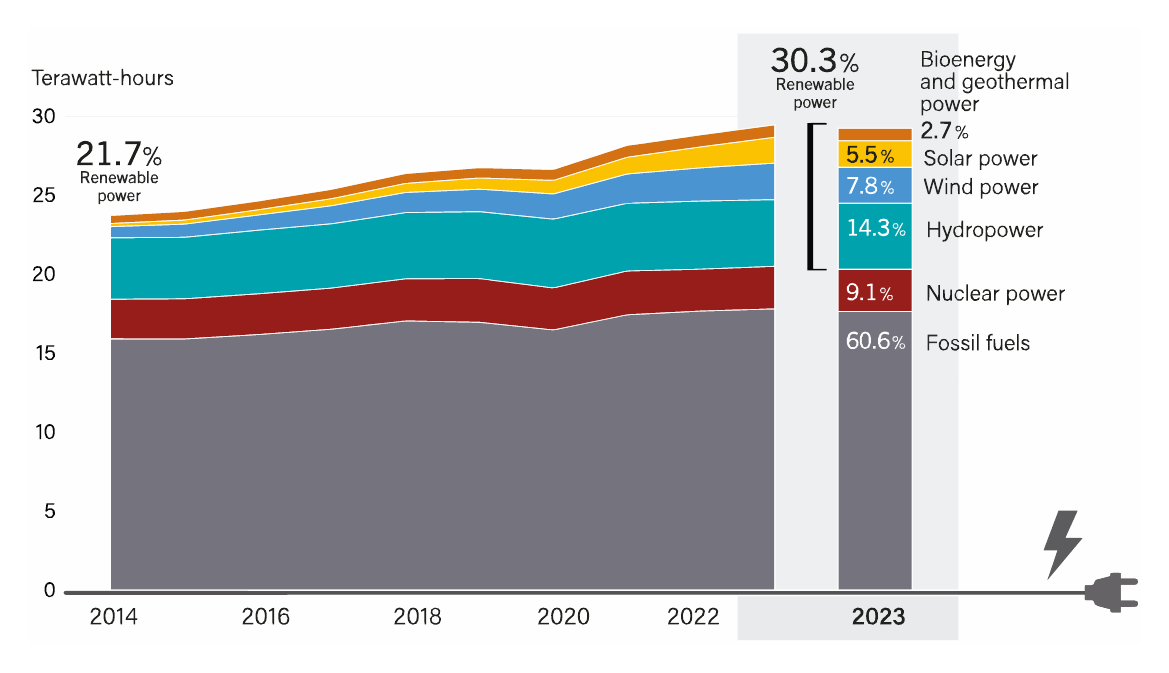
\begin{tikzpicture}[y=1cm, x=1cm, yscale=\globalscale,xscale=\globalscale, every node/.append style={scale=\globalscale}, inner sep=0pt, outer sep=0pt]
  \path[fill=cfefefe] (0.0, 97.9488).. controls (58.316, 97.9488) and (116.632, 97.9488) .. (176.7152, 97.9488).. controls (176.7152, 65.6257) and (176.7152, 33.3026) .. (176.7152, 0.0).. controls (118.3992, 0.0) and (60.0832, 0.0) .. (0.0, 0.0).. controls (0.0, 32.3231) and (0.0, 64.6462) .. (0.0, 97.9488) -- cycle;



  \path[fill=c75747e,shift={(118.5069, -44.7675)}] (0.0, 97.9488).. controls (0.0, 83.2977) and (0.0, 68.6467) .. (0.0, 53.5517).. controls (-34.7416, 53.5517) and (-69.4833, 53.5517) .. (-105.2777, 53.5517).. controls (-105.2777, 66.6398) and (-105.2777, 79.728) .. (-105.2777, 93.2127).. controls (-101.3574, 93.2127) and (-97.437, 93.2127) .. (-93.3979, 93.2127).. controls (-91.7723, 93.3103) and (-91.7723, 93.3103) .. (-90.1468, 93.4107).. controls (-89.0799, 93.4776) and (-88.0128, 93.5407) .. (-86.9456, 93.6027).. controls (-86.7693, 93.613) and (-86.593, 93.6233) .. (-86.4167, 93.6335).. controls (-86.3196, 93.6392) and (-86.2224, 93.6448) .. (-86.1253, 93.6505).. controls (-86.0867, 93.6527) and (-86.0482, 93.655) .. (-86.0096, 93.6572).. controls (-85.9329, 93.6617) and (-85.8562, 93.6662) .. (-85.7795, 93.6706).. controls (-85.5755, 93.6825) and (-85.3715, 93.6944) .. (-85.1675, 93.7063).. controls (-85.0497, 93.7131) and (-84.9319, 93.72) .. (-84.8141, 93.7269).. controls (-82.7498, 93.8471) and (-80.6878, 93.9887) .. (-78.626, 94.1451).. controls (-77.9708, 94.1948) and (-77.3156, 94.2427) .. (-76.6602, 94.2881).. controls (-75.9289, 94.3388) and (-75.1979, 94.3936) .. (-74.4669, 94.449).. controls (-73.6785, 94.5089) and (-72.89, 94.5669) .. (-72.1012, 94.621).. controls (-71.9228, 94.6333) and (-71.7445, 94.6459) .. (-71.5661, 94.6587).. controls (-71.4731, 94.6654) and (-71.3802, 94.672) .. (-71.2872, 94.6785).. controls (-70.4593, 94.7369) and (-69.6357, 94.8156) .. (-68.8115, 94.9123).. controls (-68.6592, 94.9301) and (-68.5069, 94.9476) .. (-68.3546, 94.9651).. controls (-68.3236, 94.9687) and (-68.2927, 94.9722) .. (-68.2609, 94.9759).. controls (-68.1983, 94.9831) and (-68.1357, 94.9903) .. (-68.0731, 94.9975).. controls (-67.9796, 95.0082) and (-67.8861, 95.019) .. (-67.7926, 95.0298).. controls (-67.2515, 95.0922) and (-66.7102, 95.1519) .. (-66.1687, 95.2109).. controls (-65.4462, 95.2895) and (-64.7238, 95.3697) .. (-64.0016, 95.4512).. controls (-63.9831, 95.4533) and (-63.9646, 95.4554) .. (-63.9455, 95.4576).. controls (-63.6603, 95.4898) and (-63.3751, 95.522) .. (-63.0899, 95.5543).. controls (-62.7893, 95.5883) and (-62.4888, 95.6222) .. (-62.1882, 95.6562).. controls (-62.1699, 95.6582) and (-62.1516, 95.6603) .. (-62.1328, 95.6624).. controls (-61.1644, 95.7718) and (-60.1957, 95.8785) .. (-59.2269, 95.9841).. controls (-59.2081, 95.9861) and (-59.1892, 95.9882) .. (-59.1697, 95.9903).. controls (-59.1171, 95.9961) and (-59.0645, 96.0017) .. (-59.0119, 96.0074).. controls (-58.9599, 96.0132) and (-58.908, 96.0192) .. (-58.8562, 96.0259).. controls (-58.6803, 96.0485) and (-58.5052, 96.0475) .. (-58.3281, 96.0473).. controls (-58.2938, 96.0473) and (-58.2594, 96.0473) .. (-58.224, 96.0474).. controls (-58.1316, 96.0474) and (-58.0391, 96.0473) .. (-57.9467, 96.0472).. controls (-57.8887, 96.0471) and (-57.8308, 96.047) .. (-57.7729, 96.047).. controls (-57.2977, 96.0465) and (-56.8229, 96.043) .. (-56.348, 96.0286).. controls (-55.9339, 96.0161) and (-55.5198, 96.0106) .. (-55.1056, 96.0049).. controls (-54.5944, 95.9978) and (-54.0833, 95.9903) .. (-53.5722, 95.976).. controls (-53.1201, 95.9634) and (-52.6678, 95.9575) .. (-52.2155, 95.9511).. controls (-51.7237, 95.9443) and (-51.232, 95.9369) .. (-50.7404, 95.923).. controls (-50.3617, 95.9125) and (-49.983, 95.9071) .. (-49.6043, 95.9022).. controls (-49.2355, 95.8973) and (-48.8668, 95.8914) .. (-48.4981, 95.885).. controls (-48.4784, 95.8847) and (-48.4588, 95.8843) .. (-48.4385, 95.884).. controls (-47.227, 95.8629) and (-46.0303, 95.803) .. (-44.8273, 95.6475).. controls (-44.6615, 95.6262) and (-44.4957, 95.6087) .. (-44.3293, 95.594).. controls (-44.3033, 95.5917) and (-44.2774, 95.5894) .. (-44.2507, 95.587).. controls (-44.2297, 95.5852) and (-44.2086, 95.5834) .. (-44.187, 95.5816).. controls (-44.0103, 95.5662) and (-43.8337, 95.5498) .. (-43.6572, 95.5329).. controls (-43.6051, 95.528) and (-43.5531, 95.5231) .. (-43.5011, 95.5183).. controls (-43.3386, 95.5028) and (-43.1773, 95.4847) .. (-43.0159, 95.4607).. controls (-42.8525, 95.4366) and (-42.6899, 95.4217) .. (-42.5252, 95.4104).. controls (-42.1777, 95.3845) and (-41.8325, 95.3446) .. (-41.4867, 95.3029).. controls (-41.0001, 95.2437) and (-41.0001, 95.2437) .. (-40.5115, 95.2056).. controls (-40.379, 95.1966) and (-40.2477, 95.1781) .. (-40.116, 95.1607).. controls (-39.7666, 95.1159) and (-39.4165, 95.0831) .. (-39.0657, 95.0516).. controls (-38.7262, 95.0211) and (-38.3872, 94.9898) .. (-38.049, 94.9459).. controls (-37.6992, 94.9005) and (-37.3483, 94.8684) .. (-36.997, 94.8366).. controls (-36.9026, 94.828) and (-36.8082, 94.8194) .. (-36.7138, 94.8107).. controls (-36.6558, 94.8054) and (-36.5978, 94.8001) .. (-36.5398, 94.7949).. controls (-36.5138, 94.7925) and (-36.4878, 94.7901) .. (-36.461, 94.7876).. controls (-36.4383, 94.7856) and (-36.4156, 94.7835) .. (-36.3922, 94.7814).. controls (-36.3254, 94.7735) and (-36.2608, 94.7606) .. (-36.195, 94.7473).. controls (-36.1333, 94.7422) and (-36.0716, 94.7378) .. (-36.0098, 94.7341).. controls (-35.901, 94.7275) and (-35.7989, 94.7158) .. (-35.6923, 94.6944).. controls (-35.2064, 94.6222) and (-34.7894, 94.6605) .. (-34.3148, 94.7754).. controls (-34.2573, 94.7886) and (-34.1997, 94.8018) .. (-34.1422, 94.8148).. controls (-34.0561, 94.8344) and (-33.9702, 94.854) .. (-33.8843, 94.874).. controls (-33.6057, 94.9388) and (-33.3255, 94.9945) .. (-33.0448, 95.0495).. controls (-32.9242, 95.0732) and (-32.8037, 95.0978) .. (-32.6832, 95.1224).. controls (-32.6606, 95.127) and (-32.6379, 95.1316) .. (-32.6146, 95.1363).. controls (-32.5453, 95.1505) and (-32.4759, 95.1647) .. (-32.4065, 95.1789).. controls (-32.382, 95.1839) and (-32.3575, 95.1889) .. (-32.3322, 95.1941).. controls (-31.9775, 95.2666) and (-31.623, 95.3404) .. (-31.2688, 95.4154).. controls (-30.9798, 95.4765) and (-30.6908, 95.5367) .. (-30.4011, 95.5941).. controls (-30.1257, 95.6487) and (-29.8506, 95.7048) .. (-29.5755, 95.761).. controls (-29.5505, 95.7661) and (-29.5255, 95.7712) .. (-29.4998, 95.7764).. controls (-29.1072, 95.8567) and (-28.7149, 95.9384) .. (-28.323, 96.0219).. controls (-28.1069, 96.0677) and (-27.8907, 96.112) .. (-27.6741, 96.155).. controls (-27.3788, 96.2137) and (-27.0839, 96.2744) .. (-26.7891, 96.3356).. controls (-26.7661, 96.3404) and (-26.7432, 96.3451) .. (-26.7196, 96.35).. controls (-26.5531, 96.3846) and (-26.3867, 96.4192) .. (-26.2202, 96.4539).. controls (-26.0306, 96.4933) and (-25.841, 96.5327) .. (-25.6514, 96.5721).. controls (-25.6171, 96.5792) and (-25.6171, 96.5792) .. (-25.5822, 96.5865).. controls (-25.2846, 96.6483) and (-24.9867, 96.7088) .. (-24.6885, 96.7677).. controls (-24.5326, 96.7987) and (-24.3776, 96.8321) .. (-24.2227, 96.8675).. controls (-23.6944, 96.9872) and (-23.1762, 97.0595) .. (-22.6352, 97.0871).. controls (-22.6104, 97.0883) and (-22.5857, 97.0896) .. (-22.5602, 97.0909).. controls (-22.3216, 97.103) and (-22.083, 97.1123) .. (-21.8442, 97.1214).. controls (-20.9977, 97.154) and (-20.1517, 97.1981) .. (-19.3057, 97.2416).. controls (-19.1482, 97.2497) and (-18.9907, 97.2577) .. (-18.8332, 97.2657).. controls (-18.7991, 97.2675) and (-18.7991, 97.2675) .. (-18.7644, 97.2693).. controls (-18.7181, 97.2716) and (-18.6719, 97.274) .. (-18.6257, 97.2763).. controls (-18.1972, 97.2982) and (-17.7687, 97.3202) .. (-17.3403, 97.3421).. controls (-16.9735, 97.3609) and (-16.6067, 97.3797) .. (-16.2399, 97.3984).. controls (-15.8109, 97.4202) and (-15.382, 97.4421) .. (-14.9531, 97.4641).. controls (-14.9074, 97.4664) and (-14.8617, 97.4688) .. (-14.816, 97.4711).. controls (-14.7935, 97.4723) and (-14.771, 97.4734) .. (-14.7479, 97.4746).. controls (-14.5902, 97.4827) and (-14.4326, 97.4907) .. (-14.275, 97.4988).. controls (-14.0834, 97.5085) and (-13.8919, 97.5183) .. (-13.7003, 97.5282).. controls (-13.6028, 97.5332) and (-13.5053, 97.5382) .. (-13.4078, 97.5431).. controls (-13.302, 97.5485) and (-13.1962, 97.554) .. (-13.0904, 97.5594).. controls (-13.0598, 97.561) and (-13.0293, 97.5625) .. (-12.9978, 97.5641).. controls (-12.847, 97.572) and (-12.6972, 97.5825) .. (-12.5471, 97.5991).. controls (-12.4375, 97.6098) and (-12.3276, 97.6122) .. (-12.2176, 97.6154).. controls (-12.1915, 97.6162) and (-12.1655, 97.6171) .. (-12.1386, 97.6179).. controls (-12.0513, 97.6207) and (-11.9641, 97.6233) .. (-11.8768, 97.6259).. controls (-11.8132, 97.6278) and (-11.7495, 97.6298) .. (-11.6859, 97.6318).. controls (-11.5294, 97.6366) and (-11.3729, 97.6414) .. (-11.2164, 97.6461).. controls (-11.0877, 97.65) and (-10.959, 97.6539) .. (-10.8303, 97.6579).. controls (-9.8619, 97.6876) and (-8.8934, 97.716) .. (-7.9249, 97.7438).. controls (-7.8464, 97.7461) and (-7.768, 97.7483) .. (-7.6895, 97.7506).. controls (-7.1988, 97.7647) and (-6.7082, 97.7787) .. (-6.2176, 97.7926).. controls (-6.0219, 97.7981) and (-5.8262, 97.8036) .. (-5.6306, 97.8092).. controls (-5.495, 97.8131) and (-5.3594, 97.8169) .. (-5.2239, 97.8207).. controls (-5.1404, 97.823) and (-5.0569, 97.8254) .. (-4.9735, 97.8278).. controls (-4.9356, 97.8289) and (-4.8977, 97.8299) .. (-4.8597, 97.831).. controls (-4.6401, 97.8369) and (-4.421, 97.8463) .. (-4.2018, 97.8602).. controls (-4.0409, 97.8704) and (-3.8802, 97.8746) .. (-3.719, 97.8768).. controls (-3.6902, 97.8773) and (-3.6614, 97.8778) .. (-3.6317, 97.8783).. controls (-3.5109, 97.8803) and (-3.3901, 97.8821) .. (-3.2693, 97.884).. controls (-2.8311, 97.8907) and (-2.8311, 97.8907) .. (-2.3934, 97.9125).. controls (-2.145, 97.9284) and (-1.8961, 97.9312) .. (-1.6473, 97.9356).. controls (-1.5609, 97.9371) and (-1.4745, 97.9389) .. (-1.3882, 97.9406).. controls (-0.9252, 97.9493) and (-0.4633, 97.9488) .. (0.0, 97.9488) -- cycle;



  \path[fill=ceeeff0,shift={(112.7125, -0.9525)}] (0.0, 97.9488).. controls (11.5602, 97.9488) and (23.1204, 97.9488) .. (35.0308, 97.9488).. controls (35.0439, 96.2331) and (35.0439, 96.2331) .. (35.0573, 94.4827).. controls (35.1359, 94.4391) and (35.2145, 94.3954) .. (35.2954, 94.3504).. controls (35.3573, 94.2852) and (35.3573, 94.2852) .. (35.3996, 94.2198).. controls (35.414, 94.1983) and (35.4285, 94.1767) .. (35.4433, 94.1546).. controls (35.5592, 93.9411) and (35.5335, 93.8197) .. (35.5335, 93.5567).. controls (35.1057, 93.5567) and (34.6779, 93.5567) .. (34.2371, 93.5567).. controls (34.3121, 93.1987) and (34.3121, 93.1987) .. (34.5546, 92.9481).. controls (34.7222, 92.8922) and (34.8928, 92.9125) .. (35.0577, 92.9711).. controls (35.1191, 93.0061) and (35.1407, 93.0383) .. (35.1764, 93.0986).. controls (35.2056, 93.1478) and (35.2056, 93.1478) .. (35.2425, 93.1863).. controls (35.324, 93.2023) and (35.3987, 93.1975) .. (35.4806, 93.1863).. controls (35.4717, 93.0436) and (35.39, 92.9432) .. (35.2954, 92.8423).. controls (35.2111, 92.7783) and (35.1393, 92.7365) .. (35.0308, 92.7365).. controls (35.0439, 90.0909) and (35.0439, 90.0909) .. (35.0573, 87.3919).. controls (35.066, 87.4093) and (35.0748, 87.4268) .. (35.0838, 87.4448).. controls (35.1711, 87.4448) and (35.2584, 87.4448) .. (35.3483, 87.4448).. controls (35.3154, 87.3346) and (35.2825, 87.2245) .. (35.2495, 87.1144).. controls (35.2383, 87.077) and (35.2271, 87.0396) .. (35.2159, 87.0021).. controls (35.1998, 86.9481) and (35.1836, 86.8942) .. (35.1675, 86.8402).. controls (35.1578, 86.8078) and (35.1481, 86.7753) .. (35.1381, 86.7419).. controls (35.1102, 86.651) and (35.1102, 86.651) .. (35.0825, 86.5852).. controls (35.0463, 86.4517) and (35.0491, 86.323) .. (35.0489, 86.1852).. controls (35.0486, 86.1545) and (35.0483, 86.1238) .. (35.0481, 86.0921).. controls (35.0472, 85.9908) and (35.0468, 85.8894) .. (35.0463, 85.788).. controls (35.0458, 85.7177) and (35.0453, 85.6473) .. (35.0448, 85.577).. controls (35.0435, 85.4108) and (35.0426, 85.2447) .. (35.0417, 85.0786).. controls (35.0407, 84.8893) and (35.0394, 84.7001) .. (35.038, 84.5109).. controls (35.0353, 84.1219) and (35.033, 83.7328) .. (35.0308, 83.3438).. controls (35.0597, 83.3402) and (35.0885, 83.3367) .. (35.1182, 83.3331).. controls (35.2465, 83.3124) and (35.33, 83.2728) .. (35.4082, 83.1658).. controls (35.483, 83.034) and (35.5062, 82.9113) .. (35.4806, 82.7617).. controls (35.4432, 82.6427) and (35.3948, 82.5674) .. (35.3004, 82.4855).. controls (35.216, 82.4442) and (35.216, 82.4442) .. (35.0308, 82.4177).. controls (35.0439, 82.0117) and (35.0439, 82.0117) .. (35.0573, 81.5975).. controls (35.1184, 81.7083) and (35.1795, 81.8191) .. (35.2425, 81.9332).. controls (35.2723, 81.9871) and (35.302, 82.041) .. (35.3318, 82.095).. controls (35.411, 82.2385) and (35.4902, 82.3821) .. (35.5694, 82.5257).. controls (35.6073, 82.5945) and (35.6452, 82.6632) .. (35.6832, 82.732).. controls (35.7012, 82.7646) and (35.7192, 82.7973) .. (35.7372, 82.8299).. controls (35.8366, 83.0102) and (35.9361, 83.1904) .. (36.0363, 83.3702).. controls (36.0974, 83.3702) and (36.1585, 83.3702) .. (36.2215, 83.3702).. controls (36.1866, 83.2376) and (36.1239, 83.1331) .. (36.0528, 83.0176).. controls (35.9597, 82.8646) and (35.8769, 82.7058) .. (35.7943, 82.547).. controls (35.6563, 82.2821) and (35.5133, 82.0206) .. (35.3653, 81.761).. controls (35.2695, 81.5929) and (35.1758, 81.4237) .. (35.0838, 81.2535).. controls (35.0663, 81.2535) and (35.0488, 81.2535) .. (35.0308, 81.2535).. controls (35.0308, 80.4503) and (35.0308, 79.647) .. (35.0308, 78.8194).. controls (35.1443, 78.8194) and (35.2578, 78.8194) .. (35.3748, 78.8194).. controls (35.5553, 78.7623) and (35.6679, 78.6881) .. (35.7717, 78.5283).. controls (35.7983, 78.4484) and (35.8022, 78.3925) .. (35.8036, 78.3088).. controls (35.8043, 78.2659) and (35.8043, 78.2659) .. (35.8052, 78.2221).. controls (35.8056, 78.1913) and (35.806, 78.1604) .. (35.8065, 78.1287).. controls (35.807, 78.0971) and (35.8076, 78.0655) .. (35.8082, 78.0329).. controls (35.8099, 77.9318) and (35.8115, 77.8307) .. (35.813, 77.7296).. controls (35.8142, 77.6612) and (35.8153, 77.5927) .. (35.8165, 77.5242).. controls (35.8193, 77.3562) and (35.822, 77.1882) .. (35.8246, 77.0202).. controls (35.746, 77.0202) and (35.6674, 77.0202) .. (35.5865, 77.0202).. controls (35.5603, 77.1119) and (35.5603, 77.1119) .. (35.5335, 77.2054).. controls (35.5162, 77.1891) and (35.5162, 77.1891) .. (35.4986, 77.1726).. controls (35.3479, 77.0362) and (35.2361, 76.9909) .. (35.0308, 76.9938).. controls (35.0318, 76.62) and (35.0334, 76.2463) .. (35.0357, 75.8725).. controls (35.0367, 75.699) and (35.0376, 75.5255) .. (35.038, 75.3519).. controls (35.0384, 75.1845) and (35.0393, 75.0171) .. (35.0406, 74.8496).. controls (35.041, 74.7857) and (35.0412, 74.7218) .. (35.0412, 74.6579).. controls (35.0413, 74.5684) and (35.042, 74.479) .. (35.0428, 74.3895).. controls (35.0427, 74.3631) and (35.0426, 74.3366) .. (35.0424, 74.3093).. controls (35.0446, 74.1633) and (35.054, 74.0843) .. (35.1631, 73.9775).. controls (35.2351, 73.8276) and (35.2228, 73.6707) .. (35.2212, 73.5081).. controls (35.2211, 73.4783) and (35.2211, 73.4486) .. (35.221, 73.418).. controls (35.2207, 73.3234) and (35.22, 73.2288) .. (35.2193, 73.1341).. controls (35.2191, 73.0699) and (35.2188, 73.0056) .. (35.2186, 72.9413).. controls (35.218, 72.784) and (35.2172, 72.6267) .. (35.216, 72.4694).. controls (35.1549, 72.4694) and (35.0938, 72.4694) .. (35.0308, 72.4694).. controls (35.0308, 70.8192) and (35.0308, 69.169) .. (35.0308, 67.4688).. controls (35.092, 67.4688) and (35.1531, 67.4688) .. (35.216, 67.4688).. controls (35.2911, 67.4417) and (35.2911, 67.4417) .. (35.3583, 67.4059).. controls (35.3921, 67.3884) and (35.3921, 67.3884) .. (35.4267, 67.3706).. controls (35.4806, 67.3365) and (35.4806, 67.3365) .. (35.5071, 67.2835).. controls (35.5158, 67.6066) and (35.5245, 67.9297) .. (35.5335, 68.2625).. controls (35.6121, 68.2625) and (35.6907, 68.2625) .. (35.7717, 68.2625).. controls (35.7717, 67.4068) and (35.7717, 66.5512) .. (35.7717, 65.6696).. controls (35.6931, 65.6696) and (35.6145, 65.6696) .. (35.5335, 65.6696).. controls (35.5248, 65.7394) and (35.5161, 65.8093) .. (35.5071, 65.8812).. controls (35.4896, 65.8616) and (35.4722, 65.842) .. (35.4542, 65.8217).. controls (35.3296, 65.6975) and (35.206, 65.6431) .. (35.0308, 65.6431).. controls (35.0308, 62.9102) and (35.0308, 60.1774) .. (35.0308, 57.3617).. controls (35.1443, 57.3617) and (35.2578, 57.3617) .. (35.3748, 57.3617).. controls (35.5781, 57.3128) and (35.7186, 57.2426) .. (35.8329, 57.0607).. controls (35.8799, 56.9597) and (35.895, 56.8892) .. (35.904, 56.7796).. controls (35.8254, 56.7796) and (35.7468, 56.7796) .. (35.6658, 56.7796).. controls (35.6511, 56.8123) and (35.6364, 56.8451) .. (35.6212, 56.8788).. controls (35.5717, 56.9777) and (35.5231, 57.0374) .. (35.4277, 57.0971).. controls (35.295, 57.1374) and (35.1561, 57.1519) .. (35.0249, 57.1005).. controls (34.8607, 57.0069) and (34.8026, 56.8969) .. (34.7332, 56.7234).. controls (34.6756, 56.4258) and (34.7099, 56.1667) .. (34.8671, 55.9065).. controls (34.9724, 55.8102) and (35.0741, 55.7782) .. (35.2144, 55.7626).. controls (35.3365, 55.7687) and (35.4381, 55.8025) .. (35.5335, 55.88).. controls (35.5872, 55.9555) and (35.6283, 56.0336) .. (35.6658, 56.1181).. controls (35.7444, 56.1181) and (35.823, 56.1181) .. (35.904, 56.1181).. controls (35.831, 55.8775) and (35.7546, 55.7351) .. (35.5419, 55.5942).. controls (35.4254, 55.5339) and (35.3107, 55.533) .. (35.1813, 55.5344).. controls (35.153, 55.5346) and (35.1248, 55.5349) .. (35.0956, 55.5351).. controls (35.0743, 55.5354) and (35.0529, 55.5357) .. (35.0308, 55.536).. controls (35.0324, 54.7365) and (35.0344, 53.937) .. (35.0369, 53.1375).. controls (35.0372, 53.0431) and (35.0375, 52.9487) .. (35.0378, 52.8544).. controls (35.0378, 52.8356) and (35.0379, 52.8168) .. (35.038, 52.7974).. controls (35.0389, 52.4931) and (35.0395, 52.1889) .. (35.0401, 51.8846).. controls (35.0407, 51.5724) and (35.0416, 51.2602) .. (35.0427, 50.948).. controls (35.0433, 50.7727) and (35.0438, 50.5973) .. (35.044, 50.4219).. controls (35.0442, 50.2569) and (35.0447, 50.0919) .. (35.0455, 49.9269).. controls (35.0457, 49.8663) and (35.0458, 49.8057) .. (35.0458, 49.7451).. controls (35.0457, 49.6624) and (35.0462, 49.5798) .. (35.0467, 49.4971).. controls (35.0466, 49.4731) and (35.0465, 49.449) .. (35.0464, 49.4243).. controls (35.0479, 49.2871) and (35.0685, 49.2022) .. (35.1367, 49.0802).. controls (35.1367, 49.0453) and (35.1367, 49.0104) .. (35.1367, 48.9744).. controls (35.054, 48.9614) and (34.9806, 48.9558) .. (34.8985, 48.9744).. controls (34.8533, 49.0248) and (34.8276, 49.0729) .. (34.7997, 49.1346).. controls (34.7537, 49.2053) and (34.7145, 49.2167) .. (34.634, 49.239).. controls (34.5549, 49.2473) and (34.5549, 49.2473) .. (34.4736, 49.2456).. controls (34.433, 49.2458) and (34.433, 49.2458) .. (34.3916, 49.246).. controls (34.3165, 49.239) and (34.2732, 49.2272) .. (34.2106, 49.186).. controls (34.1653, 49.1084) and (34.1574, 49.0611) .. (34.161, 48.9711).. controls (34.1894, 48.8777) and (34.2068, 48.8648) .. (34.29, 48.8156).. controls (34.3862, 48.7829) and (34.485, 48.7602) .. (34.5835, 48.7358).. controls (34.7972, 48.6804) and (34.9858, 48.6057) .. (35.129, 48.4315).. controls (35.2026, 48.2899) and (35.1921, 48.1155) .. (35.1457, 47.9654).. controls (35.1222, 47.9167) and (35.0957, 47.875) .. (35.0573, 47.8367).. controls (35.0546, 47.7539) and (35.0537, 47.6718) .. (35.0538, 47.5891).. controls (35.0538, 47.5626) and (35.0537, 47.5361) .. (35.0537, 47.5088).. controls (35.0535, 47.4187) and (35.0536, 47.3285) .. (35.0536, 47.2384).. controls (35.0536, 47.1734) and (35.0535, 47.1084) .. (35.0534, 47.0434).. controls (35.0532, 46.9009) and (35.0532, 46.7584) .. (35.0531, 46.6159).. controls (35.0531, 46.4026) and (35.053, 46.1892) .. (35.0528, 45.9759).. controls (35.0524, 45.6125) and (35.0522, 45.249) .. (35.0521, 44.8855).. controls (35.052, 44.5169) and (35.0518, 44.1484) .. (35.0515, 43.7798).. controls (35.0515, 43.7565) and (35.0515, 43.7333) .. (35.0514, 43.7094).. controls (35.0513, 43.5909) and (35.0513, 43.4724) .. (35.0512, 43.3539).. controls (35.0505, 42.4952) and (35.05, 41.6366) .. (35.0496, 40.7779).. controls (35.0492, 39.9273) and (35.0487, 39.0766) .. (35.0481, 38.226).. controls (35.0481, 38.1864) and (35.0481, 38.1864) .. (35.0481, 38.146).. controls (35.0479, 37.905) and (35.0477, 37.6639) .. (35.0476, 37.4228).. controls (35.0472, 36.8235) and (35.0468, 36.2242) .. (35.0464, 35.6248).. controls (35.0464, 35.5839) and (35.0464, 35.5839) .. (35.0463, 35.5421).. controls (35.0455, 34.2136) and (35.0447, 32.8851) .. (35.044, 31.5566).. controls (35.0437, 31.0954) and (35.0435, 30.6343) .. (35.0432, 30.1731).. controls (35.0432, 30.1445) and (35.0432, 30.1159) .. (35.0432, 30.0865).. controls (35.0424, 28.7575) and (35.0416, 27.4285) .. (35.0407, 26.0996).. controls (35.0407, 26.0133) and (35.0406, 25.9271) .. (35.0406, 25.8408).. controls (35.0402, 25.2692) and (35.0398, 24.6976) .. (35.0395, 24.126).. controls (35.0388, 22.9886) and (35.038, 21.8513) .. (35.0373, 20.7139).. controls (35.0373, 20.6597) and (35.0373, 20.6055) .. (35.0372, 20.5514).. controls (35.0362, 18.8826) and (35.0352, 17.2137) .. (35.0342, 15.5449).. controls (35.0341, 15.4776) and (35.0341, 15.4103) .. (35.0341, 15.343).. controls (35.033, 13.4742) and (35.0319, 11.6054) .. (35.0308, 9.7367).. controls (32.6472, 9.7367) and (30.2636, 9.7367) .. (27.8077, 9.7367).. controls (27.8077, 33.931) and (27.8077, 58.1253) .. (27.8077, 83.0527).. controls (23.8525, 83.0527) and (19.8972, 83.0527) .. (15.8221, 83.0527).. controls (15.8221, 58.8584) and (15.8221, 34.6641) .. (15.8221, 9.7367).. controls (12.5915, 9.7367) and (9.361, 9.7367) .. (6.0325, 9.7367).. controls (6.0325, 34.1143) and (6.0325, 58.492) .. (6.0325, 83.6083).. controls (5.8055, 83.5734) and (5.5785, 83.5385) .. (5.3446, 83.5025).. controls (5.0006, 83.4628) and (5.0006, 83.4628) .. (4.8286, 83.4438).. controls (4.6559, 83.4239) and (4.4844, 83.3977) .. (4.3127, 83.3702).. controls (4.0553, 83.3291) and (3.7979, 83.2965) .. (3.5388, 83.2682).. controls (3.3372, 83.2457) and (3.1372, 83.217) .. (2.9369, 83.185).. controls (2.708, 83.1484) and (2.4794, 83.1176) .. (2.249, 83.0924).. controls (1.9546, 83.0602) and (1.6626, 83.0171) .. (1.3701, 82.9709).. controls (1.2211, 82.9473) and (1.0719, 82.9264) .. (0.9221, 82.9073).. controls (0.8397, 82.8965) and (0.7575, 82.885) .. (0.6753, 82.8732).. controls (0.6495, 82.8695) and (0.6238, 82.8659) .. (0.5973, 82.8621).. controls (0.5467, 82.8549) and (0.4963, 82.8476) .. (0.4458, 82.8401).. controls (0.4223, 82.8368) and (0.3989, 82.8335) .. (0.3748, 82.8301).. controls (0.3541, 82.8271) and (0.3335, 82.8241) .. (0.3123, 82.821).. controls (0.2086, 82.812) and (0.1041, 82.8146) .. (0.0, 82.8146).. controls (0.0, 83.4694) and (0.0, 84.1243) .. (0.0, 84.799).. controls (-35.2131, 84.799) and (-70.4263, 84.799) .. (-106.7065, 84.799).. controls (-106.6977, 84.8252) and (-106.689, 84.8513) .. (-106.68, 84.8783).. controls (-71.4756, 84.8783) and (-36.2712, 84.8783) .. (0.0, 84.8783).. controls (0.0, 89.1916) and (0.0, 93.5048) .. (0.0, 97.9488) -- cycle;



  \path[fill=c00a2ae,shift={(118.5069, -27.4108)}] (0.0, 97.9488).. controls (0.0, 94.5261) and (0.0, 91.1035) .. (0.0, 87.5771).. controls (-0.3868, 87.5473) and (-0.3868, 87.5473) .. (-0.5572, 87.5416).. controls (-0.5853, 87.5406) and (-0.5853, 87.5406) .. (-0.614, 87.5396).. controls (-0.6543, 87.5382) and (-0.6945, 87.5369) .. (-0.7347, 87.5355).. controls (-0.7999, 87.5334) and (-0.8651, 87.5312) .. (-0.9302, 87.5289).. controls (-1.0243, 87.5256) and (-1.1183, 87.5224) .. (-1.2124, 87.5192).. controls (-1.463, 87.5107) and (-1.7136, 87.5019) .. (-1.9642, 87.4931).. controls (-1.9896, 87.4922) and (-2.015, 87.4913) .. (-2.0412, 87.4903).. controls (-2.5476, 87.4724) and (-3.054, 87.4517) .. (-3.5603, 87.4299).. controls (-3.5997, 87.4282) and (-3.639, 87.4265) .. (-3.6784, 87.4248).. controls (-3.8305, 87.4183) and (-3.9826, 87.4117) .. (-4.1347, 87.4052).. controls (-4.4559, 87.3913) and (-4.777, 87.378) .. (-5.0982, 87.3654).. controls (-5.1237, 87.3644) and (-5.1492, 87.3634) .. (-5.1755, 87.3624).. controls (-5.5602, 87.3473) and (-5.9449, 87.3335) .. (-6.3296, 87.3199).. controls (-6.3533, 87.3191) and (-6.3771, 87.3183) .. (-6.4015, 87.3174).. controls (-6.5975, 87.3105) and (-6.7935, 87.3036) .. (-6.9896, 87.2967).. controls (-7.5674, 87.2763) and (-8.1451, 87.2554) .. (-8.7226, 87.2283).. controls (-9.1937, 87.2063) and (-9.6649, 87.19) .. (-10.1363, 87.1745).. controls (-10.1955, 87.1726) and (-10.2547, 87.1706) .. (-10.3139, 87.1686).. controls (-10.3608, 87.1671) and (-10.3608, 87.1671) .. (-10.4087, 87.1655).. controls (-10.6192, 87.1584) and (-10.8297, 87.1503) .. (-11.0402, 87.1417).. controls (-11.8856, 87.1072) and (-12.7309, 87.0844) .. (-13.5768, 87.0663).. controls (-13.919, 87.059) and (-14.2612, 87.0512) .. (-14.6035, 87.0434).. controls (-14.6615, 87.0421) and (-14.7196, 87.0408) .. (-14.7777, 87.0395).. controls (-15.5106, 87.023) and (-16.2435, 87.0038) .. (-16.9763, 86.9834).. controls (-17.2118, 86.9769) and (-17.4473, 86.9704) .. (-17.6828, 86.9639).. controls (-17.7286, 86.9626) and (-17.7286, 86.9626) .. (-17.7752, 86.9614).. controls (-18.3819, 86.9447) and (-18.9886, 86.9295) .. (-19.5953, 86.9145).. controls (-19.6435, 86.9133) and (-19.6918, 86.9121) .. (-19.74, 86.9109).. controls (-20.1955, 86.8996) and (-20.6511, 86.8883) .. (-21.1066, 86.8772).. controls (-21.2872, 86.8728) and (-21.4677, 86.8684) .. (-21.6483, 86.8639).. controls (-21.7532, 86.8613) and (-21.8582, 86.8588) .. (-21.9632, 86.8562).. controls (-22.3429, 86.8471) and (-22.7226, 86.8376) .. (-23.1021, 86.8233).. controls (-23.1287, 86.8224) and (-23.1553, 86.8214) .. (-23.1826, 86.8205).. controls (-23.3673, 86.8131) and (-23.5416, 86.7928) .. (-23.7215, 86.7486).. controls (-23.7479, 86.7427) and (-23.7742, 86.7367) .. (-23.8013, 86.7306).. controls (-23.8758, 86.7135) and (-23.95, 86.6957) .. (-24.0242, 86.6775).. controls (-24.0426, 86.673) and (-24.0611, 86.6686) .. (-24.0801, 86.6639).. controls (-24.1617, 86.6441) and (-24.2431, 86.6235) .. (-24.3244, 86.6026).. controls (-24.4803, 86.5629) and (-24.6369, 86.5264) .. (-24.7935, 86.4897).. controls (-24.8442, 86.4778) and (-24.895, 86.4659) .. (-24.9457, 86.4539).. controls (-25.1456, 86.4072) and (-25.3457, 86.3647) .. (-25.5473, 86.3261).. controls (-25.64, 86.3067) and (-25.7305, 86.283) .. (-25.8217, 86.2575).. controls (-25.9968, 86.2093) and (-26.1729, 86.1713) .. (-26.3508, 86.1351).. controls (-26.5597, 86.0925) and (-26.7663, 86.0464) .. (-26.9727, 85.9934).. controls (-27.237, 85.9262) and (-27.5032, 85.8668) .. (-27.7689, 85.8053).. controls (-27.8744, 85.7809) and (-27.9799, 85.7563) .. (-28.0854, 85.7318).. controls (-28.177, 85.7104) and (-28.2686, 85.6892) .. (-28.3602, 85.6679).. controls (-28.4046, 85.6576) and (-28.449, 85.6473) .. (-28.4933, 85.637).. controls (-28.7376, 85.5801) and (-28.9819, 85.5257) .. (-29.2284, 85.4787).. controls (-29.3199, 85.4596) and (-29.4093, 85.436) .. (-29.4994, 85.4108).. controls (-29.6702, 85.3638) and (-29.8418, 85.3268) .. (-30.0153, 85.2917).. controls (-30.2291, 85.2484) and (-30.4408, 85.2005) .. (-30.652, 85.1462).. controls (-30.9055, 85.0812) and (-31.1602, 85.0231) .. (-31.416, 84.9676).. controls (-31.4342, 84.9637) and (-31.4525, 84.9597) .. (-31.4713, 84.9556).. controls (-31.5906, 84.9298) and (-31.71, 84.904) .. (-31.8294, 84.8783).. controls (-32.0522, 84.8302) and (-32.2743, 84.782) .. (-32.4941, 84.7212).. controls (-32.6632, 84.675) and (-32.8333, 84.6386) .. (-33.0051, 84.6038).. controls (-33.2189, 84.5605) and (-33.4305, 84.5126) .. (-33.6418, 84.4583).. controls (-33.9407, 84.3815) and (-34.2416, 84.3152) .. (-34.5434, 84.2505).. controls (-34.5612, 84.2467) and (-34.5789, 84.2429) .. (-34.5972, 84.239).. controls (-34.6456, 84.2286) and (-34.6941, 84.2182) .. (-34.7425, 84.2079).. controls (-34.8203, 84.1915) and (-34.8203, 84.1915) .. (-34.8985, 84.164).. controls (-35.2111, 84.1447) and (-35.5184, 84.1843) .. (-35.8279, 84.2235).. controls (-35.8776, 84.2296) and (-35.9273, 84.2357) .. (-35.9771, 84.2418).. controls (-36.2784, 84.2789) and (-36.5793, 84.3191) .. (-36.8799, 84.3619).. controls (-37.1582, 84.4011) and (-37.4372, 84.4339) .. (-37.7164, 84.4666).. controls (-38.0696, 84.5079) and (-38.4223, 84.5518) .. (-38.7747, 84.6005).. controls (-39.1226, 84.6486) and (-39.4709, 84.6921) .. (-39.8198, 84.7328).. controls (-40.1887, 84.7759) and (-40.5568, 84.8225) .. (-40.9247, 84.8734).. controls (-41.2762, 84.9218) and (-41.6282, 84.9645) .. (-41.9806, 85.0056).. controls (-42.3307, 85.0466) and (-42.68, 85.0916) .. (-43.0292, 85.1397).. controls (-43.3173, 85.1794) and (-43.6055, 85.2157) .. (-43.8944, 85.2488).. controls (-44.2237, 85.2865) and (-44.5521, 85.3291) .. (-44.8805, 85.3745).. controls (-45.2789, 85.4294) and (-45.6779, 85.4774) .. (-46.0774, 85.5236).. controls (-46.1003, 85.5263) and (-46.1231, 85.5289) .. (-46.1467, 85.5317).. controls (-46.1894, 85.5367) and (-46.2322, 85.5416) .. (-46.275, 85.5465).. controls (-46.4236, 85.5638) and (-46.4236, 85.5638) .. (-46.4942, 85.5801).. controls (-46.5861, 85.5961) and (-46.6761, 85.5964) .. (-46.7691, 85.5962).. controls (-46.7893, 85.5962) and (-46.8096, 85.5963) .. (-46.8305, 85.5964).. controls (-46.8987, 85.5965) and (-46.9669, 85.5965) .. (-47.035, 85.5964).. controls (-47.0843, 85.5965) and (-47.1336, 85.5966) .. (-47.1829, 85.5967).. controls (-47.3185, 85.5969) and (-47.4542, 85.5969) .. (-47.5898, 85.5969).. controls (-47.736, 85.597) and (-47.8823, 85.5972) .. (-48.0285, 85.5974).. controls (-48.3484, 85.5977) and (-48.6683, 85.5979) .. (-48.9882, 85.598).. controls (-49.1881, 85.5981) and (-49.388, 85.5982) .. (-49.5878, 85.5983).. controls (-50.1414, 85.5986) and (-50.6951, 85.5989) .. (-51.2487, 85.599).. controls (-51.2845, 85.599) and (-51.3203, 85.599) .. (-51.3561, 85.599).. controls (-51.3919, 85.599) and (-51.4278, 85.599) .. (-51.4637, 85.599).. controls (-51.5357, 85.599) and (-51.6077, 85.5991) .. (-51.6797, 85.5991).. controls (-51.6975, 85.5991) and (-51.7154, 85.5991) .. (-51.7338, 85.5991).. controls (-52.3118, 85.5992) and (-52.8898, 85.5996) .. (-53.4679, 85.6002).. controls (-54.0795, 85.6009) and (-54.6911, 85.6012) .. (-55.3027, 85.6013).. controls (-55.6359, 85.6013) and (-55.9691, 85.6014) .. (-56.3023, 85.6019).. controls (-56.5861, 85.6023) and (-56.87, 85.6025) .. (-57.1539, 85.6022).. controls (-57.2986, 85.6021) and (-57.4433, 85.6022) .. (-57.588, 85.6025).. controls (-57.7208, 85.6029) and (-57.8536, 85.6028) .. (-57.9865, 85.6025).. controls (-58.0342, 85.6025) and (-58.0819, 85.6025) .. (-58.1296, 85.6028).. controls (-58.4426, 85.6042) and (-58.7402, 85.5749) .. (-59.0488, 85.523).. controls (-59.1903, 85.4999) and (-59.3328, 85.4834) .. (-59.4751, 85.4657).. controls (-59.5082, 85.4616) and (-59.5413, 85.4574) .. (-59.5755, 85.4531).. controls (-59.6657, 85.4418) and (-59.7559, 85.4305) .. (-59.846, 85.4193).. controls (-59.9442, 85.4071) and (-60.0423, 85.3947) .. (-60.1403, 85.3824).. controls (-60.3103, 85.3611) and (-60.4802, 85.3399) .. (-60.6501, 85.3186).. controls (-60.8986, 85.2876) and (-61.147, 85.2565) .. (-61.3954, 85.2254).. controls (-61.8022, 85.1744) and (-62.209, 85.1235) .. (-62.6158, 85.0726).. controls (-63.0044, 85.024) and (-63.393, 84.9754) .. (-63.7815, 84.9268).. controls (-63.8052, 84.9238) and (-63.8289, 84.9208) .. (-63.8533, 84.9178).. controls (-64.1142, 84.8851) and (-64.3752, 84.8524) .. (-64.6362, 84.8197).. controls (-64.7067, 84.8109) and (-64.7771, 84.8021) .. (-64.8476, 84.7933).. controls (-64.8943, 84.7874) and (-64.9411, 84.7816) .. (-64.9879, 84.7757).. controls (-65.2885, 84.7381) and (-65.5891, 84.7004) .. (-65.8898, 84.6628).. controls (-66.1136, 84.6349) and (-66.3374, 84.6069) .. (-66.5612, 84.5788).. controls (-66.5827, 84.5761) and (-66.6043, 84.5734) .. (-66.6266, 84.5707).. controls (-67.1708, 84.5025) and (-67.715, 84.434) .. (-68.2591, 84.3646).. controls (-68.3498, 84.3531) and (-68.4406, 84.3415) .. (-68.5313, 84.33).. controls (-68.7698, 84.2996) and (-69.0083, 84.2692) .. (-69.2467, 84.2385).. controls (-69.9783, 84.1442) and (-70.7093, 84.0708) .. (-71.4452, 84.0197).. controls (-71.6712, 84.0038) and (-71.8971, 83.9868) .. (-72.123, 83.9698).. controls (-72.208, 83.9634) and (-72.293, 83.957) .. (-72.378, 83.9506).. controls (-72.4103, 83.9481) and (-72.4103, 83.9481) .. (-72.4432, 83.9457).. controls (-72.5981, 83.934) and (-72.753, 83.9225) .. (-72.9079, 83.911).. controls (-73.6373, 83.8569) and (-74.3663, 83.7992) .. (-75.0954, 83.7406).. controls (-75.1522, 83.7361) and (-75.209, 83.7315) .. (-75.2658, 83.7269).. controls (-75.4897, 83.7089) and (-75.7136, 83.6909) .. (-75.9375, 83.6729).. controls (-76.4417, 83.6323) and (-76.9459, 83.592) .. (-77.4502, 83.5521).. controls (-77.4702, 83.5505) and (-77.4903, 83.5489) .. (-77.5109, 83.5473).. controls (-78.2199, 83.4912) and (-78.929, 83.4377) .. (-79.6382, 83.3851).. controls (-80.0931, 83.3513) and (-80.548, 83.3171) .. (-81.0027, 83.2798).. controls (-81.021, 83.2783) and (-81.0392, 83.2768) .. (-81.058, 83.2752).. controls (-81.1475, 83.2679) and (-81.237, 83.2605) .. (-81.3265, 83.2531).. controls (-81.8261, 83.2119) and (-82.325, 83.1738) .. (-82.8257, 83.1497).. controls (-83.0965, 83.1365) and (-83.3663, 83.1169) .. (-83.6364, 83.094).. controls (-84.0056, 83.0629) and (-84.3748, 83.035) .. (-84.7444, 83.0097).. controls (-84.7681, 83.0081) and (-84.7918, 83.0064) .. (-84.8162, 83.0047).. controls (-85.1044, 82.9847) and (-85.3925, 82.9679) .. (-85.6812, 82.9566).. controls (-85.8403, 82.9501) and (-85.9981, 82.9376) .. (-86.1566, 82.9221).. controls (-86.3736, 82.9009) and (-86.5905, 82.8855) .. (-86.8082, 82.8731).. controls (-87.142, 82.854) and (-87.4755, 82.8321) .. (-87.8089, 82.8079).. controls (-87.8284, 82.8065) and (-87.8479, 82.805) .. (-87.8679, 82.8036).. controls (-88.0466, 82.7906) and (-88.2252, 82.7775) .. (-88.4038, 82.7644).. controls (-88.5224, 82.7556) and (-88.6411, 82.747) .. (-88.7598, 82.7384).. controls (-88.7787, 82.737) and (-88.7977, 82.7357) .. (-88.8172, 82.7343).. controls (-89.0741, 82.7158) and (-89.331, 82.7) .. (-89.5884, 82.6906).. controls (-89.7416, 82.6848) and (-89.8934, 82.6724) .. (-90.046, 82.6575).. controls (-90.263, 82.6363) and (-90.4799, 82.621) .. (-90.6976, 82.6085).. controls (-91.0314, 82.5894) and (-91.3649, 82.5675) .. (-91.6983, 82.5433).. controls (-91.7178, 82.5419) and (-91.7372, 82.5405) .. (-91.7573, 82.539).. controls (-91.9359, 82.526) and (-92.1146, 82.5129) .. (-92.2932, 82.4998).. controls (-92.3928, 82.4924) and (-92.4925, 82.4852) .. (-92.5921, 82.478).. controls (-92.6463, 82.474) and (-92.7004, 82.47) .. (-92.7545, 82.466).. controls (-93.3055, 82.4261) and (-93.8555, 82.4131) .. (-94.4078, 82.4098).. controls (-94.4811, 82.4093) and (-94.5544, 82.4088) .. (-94.6276, 82.4083).. controls (-94.8054, 82.407) and (-94.9832, 82.4058) .. (-95.1609, 82.4047).. controls (-95.3074, 82.4038) and (-95.4539, 82.4028) .. (-95.6004, 82.4019).. controls (-95.6321, 82.4016) and (-95.6321, 82.4016) .. (-95.6644, 82.4014).. controls (-95.7074, 82.4011) and (-95.7505, 82.4008) .. (-95.7935, 82.4005).. controls (-96.1971, 82.3978) and (-96.6006, 82.3952) .. (-97.0042, 82.3927).. controls (-97.3417, 82.3905) and (-97.6792, 82.3883) .. (-98.0167, 82.3859).. controls (-98.4145, 82.3832) and (-98.8124, 82.3805) .. (-99.2102, 82.378).. controls (-99.2539, 82.3777) and (-99.2977, 82.3774) .. (-99.3414, 82.3771).. controls (-99.3629, 82.377) and (-99.3844, 82.3768) .. (-99.4065, 82.3767).. controls (-99.5274, 82.3759) and (-99.6483, 82.3751) .. (-99.7692, 82.3742).. controls (-101.5966, 82.3615) and (-103.4237, 82.3648) .. (-105.2513, 82.3648).. controls (-105.2513, 85.508) and (-105.2513, 88.6513) .. (-105.2513, 91.8898).. controls (-102.3792, 91.9217) and (-102.3792, 91.9217) .. (-101.6242, 91.9293).. controls (-101.5957, 91.9296) and (-101.5671, 91.9298) .. (-101.5378, 91.9301).. controls (-100.6575, 91.939) and (-99.7772, 91.9462) .. (-98.8969, 91.9512).. controls (-98.858, 91.9514) and (-98.858, 91.9514) .. (-98.8183, 91.9516).. controls (-98.2751, 91.9547) and (-97.7319, 91.9574) .. (-97.1886, 91.9598).. controls (-96.6616, 91.9622) and (-96.1347, 91.965) .. (-95.6077, 91.9687).. controls (-95.5627, 91.969) and (-95.5177, 91.9693) .. (-95.4728, 91.9696).. controls (-95.1724, 91.9717) and (-94.872, 91.9742) .. (-94.5716, 91.9774).. controls (-94.4855, 91.9782) and (-94.3993, 91.979) .. (-94.3132, 91.9796).. controls (-93.5733, 91.985) and (-92.8489, 92.0468) .. (-92.1137, 92.1324).. controls (-91.9066, 92.156) and (-91.6992, 92.1757) .. (-91.4917, 92.1946).. controls (-91.4738, 92.1962) and (-91.4559, 92.1978) .. (-91.4375, 92.1995).. controls (-91.3467, 92.2077) and (-91.2559, 92.2159) .. (-91.1652, 92.224).. controls (-90.9859, 92.24) and (-90.8066, 92.2564) .. (-90.6273, 92.2729).. controls (-90.6097, 92.2745) and (-90.592, 92.2762) .. (-90.5738, 92.2778).. controls (-90.2991, 92.3031) and (-90.0244, 92.3298) .. (-89.7499, 92.3575).. controls (-89.7317, 92.3593) and (-89.7135, 92.3611) .. (-89.6948, 92.363).. controls (-89.5042, 92.3822) and (-89.3137, 92.4016) .. (-89.1231, 92.4212).. controls (-88.8432, 92.4498) and (-88.5643, 92.4762) .. (-88.2833, 92.4917).. controls (-88.1592, 92.5001) and (-88.036, 92.5138) .. (-87.9125, 92.5281).. controls (-87.6148, 92.5625) and (-87.3166, 92.5917) .. (-87.0184, 92.6216).. controls (-86.9476, 92.6287) and (-86.8767, 92.6359) .. (-86.8059, 92.6431).. controls (-86.4686, 92.6774) and (-86.132, 92.7116) .. (-85.7935, 92.7301).. controls (-85.6706, 92.7383) and (-85.5486, 92.7523) .. (-85.4263, 92.7665).. controls (-85.1063, 92.8034) and (-84.7854, 92.8318) .. (-84.4647, 92.862).. controls (-84.3221, 92.8754) and (-84.1794, 92.8889) .. (-84.0368, 92.9025).. controls (-84.0012, 92.9058) and (-83.9655, 92.9092) .. (-83.9299, 92.9126).. controls (-83.4516, 92.9578) and (-82.9735, 93.0039) .. (-82.4954, 93.0512).. controls (-81.7337, 93.1265) and (-80.9716, 93.1941) .. (-80.2088, 93.2571).. controls (-80.1137, 93.2649) and (-80.0186, 93.2728) .. (-79.9235, 93.2807).. controls (-79.8958, 93.283) and (-79.8958, 93.283) .. (-79.8675, 93.2854).. controls (-79.5569, 93.3113) and (-79.2466, 93.3403) .. (-78.9364, 93.3712).. controls (-78.73, 93.3918) and (-78.5236, 93.4093) .. (-78.3167, 93.4244).. controls (-78.0472, 93.4442) and (-77.7785, 93.4691) .. (-77.5097, 93.4958).. controls (-77.2822, 93.5183) and (-77.0548, 93.5385) .. (-76.8267, 93.555).. controls (-76.5253, 93.577) and (-76.2246, 93.6053) .. (-75.9238, 93.6344).. controls (-75.5877, 93.6669) and (-75.2516, 93.6986) .. (-74.9151, 93.727).. controls (-74.897, 93.7285) and (-74.8789, 93.7301) .. (-74.8602, 93.7316).. controls (-74.8324, 93.734) and (-74.8324, 93.734) .. (-74.804, 93.7364).. controls (-74.7651, 93.7396) and (-74.7262, 93.7429) .. (-74.6872, 93.7462).. controls (-74.6672, 93.7479) and (-74.6472, 93.7496) .. (-74.6265, 93.7513).. controls (-74.4511, 93.7662) and (-74.2758, 93.7816) .. (-74.1004, 93.7971).. controls (-74.0711, 93.7997) and (-74.0417, 93.8022) .. (-74.0115, 93.8049).. controls (-73.9501, 93.8103) and (-73.8887, 93.8158) .. (-73.8273, 93.8212).. controls (-73.3633, 93.8621) and (-72.8992, 93.9025) .. (-72.4351, 93.9417).. controls (-72.4145, 93.9434) and (-72.394, 93.9451) .. (-72.3728, 93.9469).. controls (-72.1896, 93.9624) and (-72.0064, 93.9778) .. (-71.8232, 93.9931).. controls (-71.7851, 93.9963) and (-71.7469, 93.9995) .. (-71.7088, 94.0027).. controls (-71.6901, 94.0042) and (-71.6714, 94.0058) .. (-71.6521, 94.0074).. controls (-71.5032, 94.0199) and (-71.3543, 94.0326) .. (-71.2055, 94.0454).. controls (-71.0962, 94.0547) and (-70.9869, 94.0637) .. (-70.8776, 94.0724).. controls (-70.3417, 94.1152) and (-69.8136, 94.1869) .. (-69.283, 94.2729).. controls (-69.1239, 94.2987) and (-68.9647, 94.324) .. (-68.8056, 94.3492).. controls (-68.7665, 94.3554) and (-68.7274, 94.3617) .. (-68.6884, 94.3679).. controls (-68.3773, 94.4174) and (-68.0657, 94.4614) .. (-67.7531, 94.5008).. controls (-67.6016, 94.5202) and (-67.4527, 94.543) .. (-67.3032, 94.5744).. controls (-67.1386, 94.6065) and (-66.9723, 94.629) .. (-66.8065, 94.6537).. controls (-66.7652, 94.6598) and (-66.7239, 94.666) .. (-66.6826, 94.6722).. controls (-66.5742, 94.6885) and (-66.4657, 94.7047) .. (-66.3572, 94.7209).. controls (-66.1856, 94.7465) and (-66.0141, 94.7723) .. (-65.8425, 94.798).. controls (-65.7797, 94.8074) and (-65.7169, 94.8168) .. (-65.6541, 94.8262).. controls (-65.3561, 94.8709) and (-65.0582, 94.9163) .. (-64.7604, 94.9623).. controls (-64.7363, 94.9661) and (-64.7122, 94.9698) .. (-64.6874, 94.9736).. controls (-64.6326, 94.9821) and (-64.5778, 94.9906) .. (-64.523, 94.9992).. controls (-64.3719, 95.0226) and (-64.221, 95.0453) .. (-64.0694, 95.0648).. controls (-64.0359, 95.0692) and (-64.0024, 95.0735) .. (-63.9678, 95.078).. controls (-63.8993, 95.0869) and (-63.8307, 95.0957) .. (-63.7622, 95.1045).. controls (-63.7287, 95.1088) and (-63.6953, 95.1132) .. (-63.6609, 95.1177).. controls (-63.6312, 95.1215) and (-63.6016, 95.1253) .. (-63.571, 95.1293).. controls (-63.4984, 95.1404) and (-63.4278, 95.1532) .. (-63.356, 95.1682).. controls (-63.1668, 95.2068) and (-62.9758, 95.2338) .. (-62.7848, 95.2622).. controls (-62.7435, 95.2684) and (-62.7022, 95.2746) .. (-62.661, 95.2808).. controls (-62.5525, 95.2971) and (-62.444, 95.3133) .. (-62.3355, 95.3295).. controls (-62.164, 95.3551) and (-61.9924, 95.3808) .. (-61.8209, 95.4065).. controls (-61.7581, 95.416) and (-61.6953, 95.4254) .. (-61.6325, 95.4348).. controls (-61.3098, 95.4831) and (-60.9874, 95.5324) .. (-60.665, 95.5823).. controls (-60.3999, 95.6233) and (-60.1347, 95.6636) .. (-59.8694, 95.7032).. controls (-59.8168, 95.7111) and (-59.7642, 95.7189) .. (-59.7116, 95.7268).. controls (-59.5836, 95.7459) and (-59.4555, 95.7651) .. (-59.3275, 95.7842).. controls (-59.255, 95.795) and (-59.1825, 95.8058) .. (-59.11, 95.8167).. controls (-59.0421, 95.8268) and (-58.9742, 95.837) .. (-58.9063, 95.8471).. controls (-58.8757, 95.8516) and (-58.845, 95.8562) .. (-58.8134, 95.861).. controls (-58.7865, 95.865) and (-58.7597, 95.869) .. (-58.732, 95.8731).. controls (-58.6868, 95.8804) and (-58.6418, 95.8887) .. (-58.5971, 95.8987).. controls (-58.5201, 95.9125) and (-58.4482, 95.9154) .. (-58.37, 95.9163).. controls (-58.3386, 95.9167) and (-58.3072, 95.9171) .. (-58.2748, 95.9175).. controls (-58.2404, 95.9178) and (-58.206, 95.9182) .. (-58.1706, 95.9185).. controls (-58.1336, 95.9189) and (-58.0966, 95.9194) .. (-58.0595, 95.9198).. controls (-57.9578, 95.921) and (-57.856, 95.9221) .. (-57.7542, 95.9231).. controls (-57.6444, 95.9242) and (-57.5346, 95.9255) .. (-57.4248, 95.9268).. controls (-57.2341, 95.9289) and (-57.0434, 95.931) .. (-56.8527, 95.933).. controls (-56.5752, 95.936) and (-56.2977, 95.9391) .. (-56.0202, 95.9422).. controls (-55.5675, 95.9473) and (-55.1149, 95.9523) .. (-54.6622, 95.9572).. controls (-54.2267, 95.962) and (-53.7911, 95.9667) .. (-53.3555, 95.9715).. controls (-53.3156, 95.972) and (-53.3156, 95.972) .. (-53.2749, 95.9724).. controls (-52.9822, 95.9757) and (-52.6895, 95.9789) .. (-52.3968, 95.9822).. controls (-52.3708, 95.9825) and (-52.3448, 95.9828) .. (-52.318, 95.9831).. controls (-52.2137, 95.9842) and (-52.1094, 95.9854) .. (-52.0051, 95.9865).. controls (-51.7038, 95.9899) and (-51.4026, 95.9932) .. (-51.1013, 95.9965).. controls (-49.192, 96.0164) and (-49.192, 96.0164) .. (-47.283, 96.0508).. controls (-46.7323, 96.0625) and (-46.1921, 96.0009) .. (-45.6459, 95.9365).. controls (-45.4327, 95.9115) and (-45.2194, 95.8907) .. (-45.0056, 95.8718).. controls (-44.6295, 95.8378) and (-44.2542, 95.7976) .. (-43.8787, 95.7571).. controls (-43.5578, 95.7226) and (-43.2369, 95.6892) .. (-42.9154, 95.6601).. controls (-42.5393, 95.626) and (-42.164, 95.5859) .. (-41.7885, 95.5455).. controls (-41.4676, 95.5109) and (-41.1467, 95.4776) .. (-40.8252, 95.4484).. controls (-40.4491, 95.4144) and (-40.0738, 95.3742) .. (-39.6983, 95.3338).. controls (-39.3774, 95.2993) and (-39.0565, 95.2659) .. (-38.735, 95.2368).. controls (-38.359, 95.2027) and (-37.9837, 95.1626) .. (-37.6084, 95.1222).. controls (-37.2489, 95.0835) and (-36.8894, 95.047) .. (-36.5293, 95.0145).. controls (-36.3401, 94.9972) and (-36.1512, 94.9781) .. (-35.9624, 94.9571).. controls (-35.9292, 94.9534) and (-35.9292, 94.9534) .. (-35.8954, 94.9497).. controls (-35.7879, 94.9377) and (-35.6805, 94.9256) .. (-35.573, 94.9132).. controls (-35.1919, 94.8697) and (-34.873, 94.888) .. (-34.5, 94.9738).. controls (-34.4351, 94.9884) and (-34.3702, 95.0029) .. (-34.3052, 95.0173).. controls (-34.2608, 95.0272) and (-34.2164, 95.0372) .. (-34.1721, 95.0471).. controls (-34.0212, 95.0808) and (-33.8701, 95.1129) .. (-33.7186, 95.1438).. controls (-33.6983, 95.1479) and (-33.678, 95.152) .. (-33.6572, 95.1562).. controls (-33.5793, 95.172) and (-33.5014, 95.1878) .. (-33.4235, 95.2034).. controls (-33.2307, 95.242) and (-33.0402, 95.2838) .. (-32.851, 95.3373).. controls (-32.7289, 95.37) and (-32.605, 95.3931) .. (-32.4809, 95.417).. controls (-32.423, 95.4284) and (-32.3652, 95.4398) .. (-32.3073, 95.4512).. controls (-32.262, 95.4601) and (-32.262, 95.4601) .. (-32.2157, 95.4693).. controls (-32.0482, 95.5024) and (-31.8809, 95.5365) .. (-31.7136, 95.5708).. controls (-31.6663, 95.5804) and (-31.6663, 95.5804) .. (-31.618, 95.5902).. controls (-31.4832, 95.6179) and (-31.3499, 95.6467) .. (-31.2176, 95.6848).. controls (-30.9729, 95.7536) and (-30.7212, 95.7955) .. (-30.4719, 95.8439).. controls (-30.229, 95.891) and (-29.9881, 95.9402) .. (-29.7487, 96.0023).. controls (-29.4509, 96.0783) and (-29.1478, 96.133) .. (-28.8465, 96.1931).. controls (-28.4515, 96.2712) and (-28.4515, 96.2712) .. (-28.0598, 96.3639).. controls (-27.8647, 96.4143) and (-27.6685, 96.4542) .. (-27.4708, 96.4922).. controls (-27.1478, 96.5545) and (-26.8273, 96.6226) .. (-26.5079, 96.7017).. controls (-26.2917, 96.7549) and (-26.0743, 96.7995) .. (-25.8558, 96.8422).. controls (-25.5975, 96.8928) and (-25.3406, 96.9487) .. (-25.0836, 97.0052).. controls (-24.9383, 97.0368) and (-24.793, 97.0677) .. (-24.6476, 97.0988).. controls (-24.3832, 97.1553) and (-24.1189, 97.2123) .. (-23.8548, 97.2699).. controls (-23.8169, 97.2781) and (-23.779, 97.2864) .. (-23.7411, 97.2946).. controls (-23.6882, 97.3061) and (-23.6354, 97.3176) .. (-23.5825, 97.3291).. controls (-23.5522, 97.3358) and (-23.5219, 97.3424) .. (-23.4906, 97.3492).. controls (-23.4142, 97.3658) and (-23.4142, 97.3658) .. (-23.3363, 97.3931).. controls (-23.2713, 97.3971) and (-23.2069, 97.3997) .. (-23.1419, 97.4012).. controls (-23.1219, 97.4017) and (-23.102, 97.4022) .. (-23.0814, 97.4028).. controls (-23.0144, 97.4046) and (-22.9473, 97.4062) .. (-22.8802, 97.4079).. controls (-22.8322, 97.4091) and (-22.7841, 97.4104) .. (-22.7361, 97.4116).. controls (-22.6325, 97.4144) and (-22.5289, 97.417) .. (-22.4253, 97.4196).. controls (-22.2611, 97.4237) and (-22.097, 97.428) .. (-21.9328, 97.4323).. controls (-21.643, 97.4399) and (-21.3532, 97.4473) .. (-21.0634, 97.4547).. controls (-20.6285, 97.4658) and (-20.1936, 97.4771) .. (-19.7587, 97.4884).. controls (-19.5959, 97.4927) and (-19.4331, 97.4968) .. (-19.2703, 97.5009).. controls (-19.1684, 97.5035) and (-19.0664, 97.5062) .. (-18.9644, 97.5088).. controls (-18.9176, 97.51) and (-18.8708, 97.5112) .. (-18.8239, 97.5124).. controls (-18.5806, 97.5184) and (-18.3378, 97.5273) .. (-18.0949, 97.5425).. controls (-17.9403, 97.5521) and (-17.7858, 97.5579) .. (-17.631, 97.5617).. controls (-17.6036, 97.5625) and (-17.5762, 97.5632) .. (-17.548, 97.564).. controls (-17.4592, 97.5663) and (-17.3703, 97.5686) .. (-17.2814, 97.5709).. controls (-17.2184, 97.5726) and (-17.1554, 97.5742) .. (-17.0924, 97.5759).. controls (-16.9273, 97.5803) and (-16.7623, 97.5846) .. (-16.5973, 97.5889).. controls (-16.334, 97.5958) and (-16.0708, 97.6027) .. (-15.8075, 97.6098).. controls (-15.7168, 97.6122) and (-15.6262, 97.6145) .. (-15.5355, 97.6168).. controls (-15.2241, 97.625) and (-14.913, 97.6354) .. (-14.6018, 97.6483).. controls (-14.3807, 97.6574) and (-14.1595, 97.6642) .. (-13.9383, 97.6695).. controls (-13.8752, 97.671) and (-13.8121, 97.6726) .. (-13.749, 97.6742).. controls (-13.5703, 97.6787) and (-13.3915, 97.6831) .. (-13.2128, 97.6875).. controls (-13.1019, 97.6902) and (-12.991, 97.693) .. (-12.8801, 97.6958).. controls (-12.8386, 97.6968) and (-12.7972, 97.6979) .. (-12.7558, 97.6988).. controls (-12.5452, 97.7038) and (-12.3352, 97.711) .. (-12.125, 97.7243).. controls (-11.9315, 97.7364) and (-11.7386, 97.7418) .. (-11.5448, 97.7436).. controls (-11.4934, 97.7442) and (-11.4419, 97.7448) .. (-11.3904, 97.7455).. controls (-11.3355, 97.7461) and (-11.2806, 97.7467) .. (-11.2257, 97.7474).. controls (-11.0218, 97.7496) and (-10.818, 97.7524) .. (-10.6142, 97.7553).. controls (-10.5927, 97.7556) and (-10.5711, 97.7559) .. (-10.5488, 97.7562).. controls (-10.0528, 97.7632) and (-9.557, 97.7748) .. (-9.0611, 97.7866).. controls (-8.1303, 97.8089) and (-7.1995, 97.827) .. (-6.2685, 97.8428).. controls (-5.4407, 97.8569) and (-4.6129, 97.8721) .. (-3.7851, 97.889).. controls (-3.7174, 97.8904) and (-3.6497, 97.8917) .. (-3.5821, 97.8931).. controls (-3.1595, 97.9017) and (-2.7369, 97.9103) .. (-2.3143, 97.9192).. controls (-2.147, 97.9227) and (-1.9797, 97.9262) .. (-1.8123, 97.9296).. controls (-1.6971, 97.9319) and (-1.582, 97.9344) .. (-1.4668, 97.9368).. controls (-1.3781, 97.9387) and (-1.2894, 97.9405) .. (-1.2007, 97.9423).. controls (-1.1712, 97.943) and (-1.1416, 97.9436) .. (-1.1111, 97.9443).. controls (-0.7407, 97.9516) and (-0.3707, 97.9488) .. (0.0, 97.9488) -- cycle;



  \path[fill=c971d1a,shift={(118.5069, -37.9942)}] (0.0, 97.9488).. controls (0.0, 95.7834) and (0.0, 93.618) .. (0.0, 91.3871).. controls (-0.4366, 91.3784) and (-0.8731, 91.3696) .. (-1.3229, 91.3606).. controls (-1.4713, 91.3519) and (-1.6198, 91.3432) .. (-1.7727, 91.3342).. controls (-1.8825, 91.3309) and (-1.992, 91.3282) .. (-2.1018, 91.3267).. controls (-2.1306, 91.3262) and (-2.1595, 91.3258) .. (-2.1892, 91.3252).. controls (-2.3099, 91.3232) and (-2.4307, 91.3214) .. (-2.5515, 91.3196).. controls (-2.9627, 91.3142) and (-2.9627, 91.3142) .. (-3.3734, 91.2945).. controls (-3.7074, 91.2719) and (-4.0425, 91.2717) .. (-4.3771, 91.2666).. controls (-4.8166, 91.2598) and (-4.8166, 91.2598) .. (-5.2554, 91.2379).. controls (-5.4924, 91.2227) and (-5.7298, 91.2215) .. (-5.9672, 91.2181).. controls (-6.4793, 91.2104) and (-6.9908, 91.1965) .. (-7.5026, 91.1754).. controls (-7.9745, 91.156) and (-8.4462, 91.1406) .. (-8.9184, 91.1315).. controls (-9.1546, 91.1269) and (-9.3905, 91.1198) .. (-9.6265, 91.1102).. controls (-9.9153, 91.0985) and (-10.2042, 91.0901) .. (-10.4932, 91.0828).. controls (-10.5146, 91.0823) and (-10.536, 91.0817) .. (-10.558, 91.0812).. controls (-10.7572, 91.0761) and (-10.9564, 91.0711) .. (-11.1556, 91.0663).. controls (-11.2661, 91.0636) and (-11.3765, 91.0608) .. (-11.4869, 91.0579).. controls (-11.5283, 91.0569) and (-11.5697, 91.0559) .. (-11.6112, 91.0549).. controls (-11.8066, 91.0503) and (-12.0007, 91.0446) .. (-12.1952, 91.0226).. controls (-12.2749, 91.014) and (-12.3545, 91.0114) .. (-12.4346, 91.0092).. controls (-12.4672, 91.0082) and (-12.4997, 91.0072) .. (-12.5333, 91.0062).. controls (-12.6339, 91.0034) and (-12.6339, 91.0034) .. (-12.7344, 91.0006).. controls (-12.767, 90.9997) and (-12.7996, 90.9987) .. (-12.8331, 90.9976).. controls (-12.8622, 90.9968) and (-12.8913, 90.996) .. (-12.9212, 90.9952).. controls (-12.9957, 90.9913) and (-13.0685, 90.9853) .. (-13.1426, 90.9773).. controls (-13.289, 90.9621) and (-13.4351, 90.9558) .. (-13.5822, 90.9505).. controls (-13.61, 90.9494) and (-13.6378, 90.9484) .. (-13.6664, 90.9473).. controls (-13.784, 90.9427) and (-13.9016, 90.9384) .. (-14.0192, 90.934).. controls (-14.1056, 90.9307) and (-14.192, 90.9274) .. (-14.2784, 90.9241).. controls (-14.3046, 90.9231) and (-14.3307, 90.9222) .. (-14.3577, 90.9212).. controls (-14.5003, 90.9157) and (-14.6414, 90.9054) .. (-14.7833, 90.8903).. controls (-14.8647, 90.8823) and (-14.9458, 90.8792) .. (-15.0275, 90.8769).. controls (-15.0601, 90.8759) and (-15.0926, 90.875) .. (-15.1262, 90.8739).. controls (-15.2268, 90.8711) and (-15.2268, 90.8711) .. (-15.3273, 90.8684).. controls (-15.3599, 90.8674) and (-15.3925, 90.8664) .. (-15.426, 90.8654).. controls (-15.4551, 90.8646) and (-15.4842, 90.8638) .. (-15.5141, 90.8629).. controls (-15.5891, 90.859) and (-15.6626, 90.8529) .. (-15.7372, 90.845).. controls (-15.8741, 90.8307) and (-16.0106, 90.8241) .. (-16.1482, 90.8192).. controls (-16.1738, 90.8182) and (-16.1994, 90.8172) .. (-16.2258, 90.8161).. controls (-16.2806, 90.814) and (-16.3354, 90.8119) .. (-16.3902, 90.8099).. controls (-16.535, 90.8044) and (-16.6798, 90.7986) .. (-16.8246, 90.7928).. controls (-16.8538, 90.7916) and (-16.883, 90.7905) .. (-16.913, 90.7893).. controls (-17.1927, 90.7779) and (-17.4723, 90.7647) .. (-17.7519, 90.7504).. controls (-17.7732, 90.7494) and (-17.7944, 90.7483) .. (-17.8164, 90.7472).. controls (-18.0785, 90.7347) and (-18.0785, 90.7347) .. (-18.3399, 90.7117).. controls (-18.5431, 90.6895) and (-18.7479, 90.6888) .. (-18.9521, 90.6831).. controls (-18.9847, 90.6822) and (-19.0173, 90.6812) .. (-19.0508, 90.6801).. controls (-19.0799, 90.6793) and (-19.109, 90.6785) .. (-19.1389, 90.6777).. controls (-19.2134, 90.6738) and (-19.2862, 90.6678) .. (-19.3603, 90.6598).. controls (-19.5067, 90.6446) and (-19.6529, 90.6383) .. (-19.7999, 90.633).. controls (-19.8277, 90.6319) and (-19.8555, 90.6309) .. (-19.8841, 90.6298).. controls (-20.0017, 90.6252) and (-20.1193, 90.6209) .. (-20.2369, 90.6165).. controls (-20.3233, 90.6132) and (-20.4097, 90.6099) .. (-20.4961, 90.6066).. controls (-20.5223, 90.6056) and (-20.5484, 90.6047) .. (-20.5754, 90.6037).. controls (-20.718, 90.5982) and (-20.8591, 90.5879) .. (-21.001, 90.5728).. controls (-21.0824, 90.5648) and (-21.1635, 90.5617) .. (-21.2452, 90.5594).. controls (-21.2778, 90.5584) and (-21.3104, 90.5575) .. (-21.3439, 90.5564).. controls (-21.4445, 90.5536) and (-21.4445, 90.5536) .. (-21.545, 90.5509).. controls (-21.5776, 90.5499) and (-21.6102, 90.5489) .. (-21.6437, 90.5479).. controls (-21.6728, 90.5471) and (-21.7019, 90.5463) .. (-21.7319, 90.5454).. controls (-21.8065, 90.5415) and (-21.8795, 90.5354) .. (-21.9537, 90.5274).. controls (-22.0972, 90.5125) and (-22.2402, 90.507) .. (-22.3843, 90.5026).. controls (-22.4397, 90.5006) and (-22.4952, 90.4987) .. (-22.5506, 90.4967).. controls (-22.6366, 90.4937) and (-22.7227, 90.4908) .. (-22.8087, 90.4882).. controls (-23.1182, 90.4786) and (-23.4067, 90.4633) .. (-23.7067, 90.3817).. controls (-23.7854, 90.3638) and (-23.8645, 90.3475) .. (-23.9436, 90.3311).. controls (-23.9875, 90.3219) and (-24.0315, 90.3127) .. (-24.0755, 90.3035).. controls (-24.1223, 90.2937) and (-24.1692, 90.2839) .. (-24.216, 90.2742).. controls (-24.2403, 90.2691) and (-24.2647, 90.264) .. (-24.2897, 90.2588).. controls (-24.8296, 90.146) and (-25.3701, 90.0358) .. (-25.9105, 89.9259).. controls (-26.1544, 89.8762) and (-26.3981, 89.8264) .. (-26.6419, 89.7764).. controls (-26.6618, 89.7723) and (-26.6818, 89.7683) .. (-26.7023, 89.7641).. controls (-26.9846, 89.7062) and (-27.2669, 89.6478) .. (-27.549, 89.5892).. controls (-27.6838, 89.5612) and (-27.8185, 89.5332) .. (-27.9532, 89.5052).. controls (-27.9866, 89.4983) and (-28.02, 89.4914) .. (-28.0545, 89.4842).. controls (-28.4564, 89.4009) and (-28.8584, 89.3192) .. (-29.2617, 89.2425).. controls (-29.5985, 89.1782) and (-29.9333, 89.1054) .. (-30.2683, 89.0323).. controls (-30.6853, 88.9413) and (-31.1025, 88.8535) .. (-31.5219, 88.7748).. controls (-31.7482, 88.7319) and (-31.973, 88.684) .. (-32.1979, 88.6347).. controls (-32.4868, 88.5715) and (-32.7765, 88.5124) .. (-33.0663, 88.4535).. controls (-33.1228, 88.442) and (-33.1793, 88.4305) .. (-33.2357, 88.419).. controls (-33.496, 88.366) and (-33.7563, 88.3134) .. (-34.0168, 88.2615).. controls (-34.0491, 88.2551) and (-34.0491, 88.2551) .. (-34.082, 88.2485).. controls (-34.1808, 88.2288) and (-34.2796, 88.2092) .. (-34.3784, 88.1898).. controls (-34.4132, 88.1829) and (-34.448, 88.176) .. (-34.4828, 88.1691).. controls (-34.5122, 88.1633) and (-34.5416, 88.1575) .. (-34.572, 88.1515).. controls (-34.6372, 88.1377) and (-34.7001, 88.1219) .. (-34.7643, 88.1044).. controls (-34.8699, 88.0778) and (-34.9723, 88.0713) .. (-35.0809, 88.0726).. controls (-35.101, 88.0727) and (-35.1211, 88.0728) .. (-35.1419, 88.0729).. controls (-35.4091, 88.0774) and (-35.6748, 88.1059) .. (-35.9404, 88.1334).. controls (-36.0298, 88.1427) and (-36.1193, 88.1516) .. (-36.2087, 88.1604).. controls (-36.47, 88.1866) and (-36.73, 88.2148) .. (-36.9896, 88.254).. controls (-37.1195, 88.2722) and (-37.2499, 88.2818) .. (-37.3807, 88.2915).. controls (-37.5825, 88.3073) and (-37.7833, 88.3258) .. (-37.9842, 88.351).. controls (-38.1618, 88.3729) and (-38.34, 88.3884) .. (-38.5184, 88.403).. controls (-38.6446, 88.4138) and (-38.7692, 88.4285) .. (-38.8944, 88.4477).. controls (-39.1964, 88.4921) and (-39.501, 88.5153) .. (-39.8049, 88.5428).. controls (-40.5204, 88.6078) and (-40.5204, 88.6078) .. (-40.8252, 88.6509).. controls (-40.9363, 88.6663) and (-41.0475, 88.6769) .. (-41.1592, 88.6867).. controls (-41.6394, 88.7308) and (-42.1188, 88.7816) .. (-42.5979, 88.8355).. controls (-42.826, 88.8612) and (-43.0542, 88.8849) .. (-43.2827, 88.9062).. controls (-43.7324, 88.9481) and (-44.1815, 88.9961) .. (-44.6302, 89.0472).. controls (-44.8861, 89.0763) and (-45.142, 89.0995) .. (-45.3987, 89.1196).. controls (-45.5614, 89.1327) and (-45.7215, 89.1523) .. (-45.8828, 89.1777).. controls (-46.0549, 89.2003) and (-46.228, 89.2124) .. (-46.401, 89.2255).. controls (-46.4274, 89.2275) and (-46.4537, 89.2296) .. (-46.4808, 89.2317).. controls (-46.5043, 89.2334) and (-46.5279, 89.2351) .. (-46.5522, 89.2369).. controls (-46.6196, 89.244) and (-46.6196, 89.244) .. (-46.6819, 89.2573).. controls (-46.7496, 89.27) and (-46.8115, 89.2744) .. (-46.8802, 89.2754).. controls (-46.9053, 89.2759) and (-46.9305, 89.2763) .. (-46.9564, 89.2768).. controls (-46.9837, 89.2771) and (-47.011, 89.2775) .. (-47.0391, 89.2779).. controls (-47.0682, 89.2783) and (-47.0972, 89.2788) .. (-47.1271, 89.2793).. controls (-47.2235, 89.2809) and (-47.3199, 89.2823) .. (-47.4163, 89.2836).. controls (-47.4842, 89.2847) and (-47.5521, 89.2858) .. (-47.6199, 89.2869).. controls (-47.7812, 89.2895) and (-47.9426, 89.292) .. (-48.1039, 89.2944).. controls (-48.4402, 89.2995) and (-48.7766, 89.3048) .. (-49.113, 89.3101).. controls (-49.1477, 89.3106) and (-49.1823, 89.3112) .. (-49.2181, 89.3118).. controls (-49.6205, 89.3181) and (-50.0227, 89.3256) .. (-50.425, 89.3367).. controls (-50.8707, 89.3489) and (-51.3165, 89.3558) .. (-51.7623, 89.3621).. controls (-51.7803, 89.3623) and (-51.7982, 89.3626) .. (-51.8167, 89.3629).. controls (-52.0024, 89.3655) and (-52.1882, 89.368) .. (-52.3739, 89.3706).. controls (-52.7887, 89.3763) and (-53.2034, 89.3822) .. (-53.6181, 89.3883).. controls (-53.6474, 89.3888) and (-53.6474, 89.3888) .. (-53.6772, 89.3892).. controls (-54.318, 89.3988) and (-54.9586, 89.4126) .. (-55.5993, 89.4307).. controls (-56.3209, 89.451) and (-57.0422, 89.4613) .. (-57.7642, 89.4621).. controls (-57.835, 89.4622) and (-57.9059, 89.4624) .. (-57.9768, 89.4627).. controls (-58.0876, 89.463) and (-58.1984, 89.463) .. (-58.3092, 89.4627).. controls (-58.3494, 89.4627) and (-58.3897, 89.4627) .. (-58.4299, 89.4628).. controls (-58.8068, 89.4638) and (-59.1734, 89.423) .. (-59.5453, 89.3634).. controls (-59.7476, 89.3334) and (-59.9511, 89.3129) .. (-60.1544, 89.2905).. controls (-60.2047, 89.2849) and (-60.2551, 89.2793) .. (-60.3054, 89.2737).. controls (-60.4111, 89.2619) and (-60.5167, 89.2502) .. (-60.6223, 89.2386).. controls (-60.7542, 89.224) and (-60.8861, 89.2093) .. (-61.0179, 89.1946).. controls (-61.5516, 89.1352) and (-62.0854, 89.0777) .. (-62.6198, 89.0251).. controls (-63.0981, 88.9779) and (-63.5757, 88.9258) .. (-64.0533, 88.8726).. controls (-64.1715, 88.8594) and (-64.2898, 88.8463) .. (-64.4081, 88.8333).. controls (-64.5014, 88.823) and (-64.5946, 88.8126) .. (-64.6879, 88.8022).. controls (-64.7316, 88.7973) and (-64.7752, 88.7925) .. (-64.8189, 88.7877).. controls (-65.0071, 88.767) and (-65.195, 88.7462) .. (-65.382, 88.7159).. controls (-65.6484, 88.6734) and (-65.9171, 88.647) .. (-66.1852, 88.6174).. controls (-66.2463, 88.6106) and (-66.3073, 88.6039) .. (-66.3683, 88.5971).. controls (-66.4964, 88.5828) and (-66.6244, 88.5686) .. (-66.7524, 88.5545).. controls (-66.9131, 88.5367) and (-67.0738, 88.5189) .. (-67.2345, 88.501).. controls (-67.869, 88.4303) and (-68.5035, 88.3604) .. (-69.139, 88.2993).. controls (-69.4021, 88.2739) and (-69.664, 88.2428) .. (-69.9261, 88.2088).. controls (-70.2705, 88.165) and (-70.6139, 88.1391) .. (-70.9606, 88.122).. controls (-70.9788, 88.1211) and (-70.9969, 88.1202) .. (-71.0157, 88.1193).. controls (-71.0646, 88.1169) and (-71.1136, 88.1146) .. (-71.1625, 88.1124).. controls (-71.2528, 88.1073) and (-71.2528, 88.1073) .. (-71.3434, 88.0932).. controls (-71.4441, 88.0788) and (-71.5443, 88.0718) .. (-71.6459, 88.0666).. controls (-71.6651, 88.0655) and (-71.6844, 88.0644) .. (-71.7042, 88.0633).. controls (-71.7858, 88.0588) and (-71.8674, 88.0544) .. (-71.9489, 88.05).. controls (-72.0089, 88.0468) and (-72.0688, 88.0434) .. (-72.1287, 88.0401).. controls (-72.1559, 88.0387) and (-72.1559, 88.0387) .. (-72.1837, 88.0373).. controls (-72.2665, 88.0326) and (-72.3476, 88.0254) .. (-72.4297, 88.0136).. controls (-72.5299, 87.9993) and (-72.6296, 87.9924) .. (-72.7307, 87.9872).. controls (-72.7499, 87.9861) and (-72.7692, 87.985) .. (-72.789, 87.9839).. controls (-72.8706, 87.9794) and (-72.9522, 87.975) .. (-73.0337, 87.9707).. controls (-73.0937, 87.9674) and (-73.1536, 87.9641) .. (-73.2135, 87.9607).. controls (-73.2407, 87.9593) and (-73.2407, 87.9593) .. (-73.2685, 87.9579).. controls (-73.3513, 87.9533) and (-73.4324, 87.946) .. (-73.5145, 87.9343).. controls (-73.6147, 87.9199) and (-73.7144, 87.913) .. (-73.8154, 87.9078).. controls (-73.8347, 87.9067) and (-73.854, 87.9057) .. (-73.8738, 87.9046).. controls (-73.9554, 87.9) and (-74.037, 87.8957) .. (-74.1185, 87.8913).. controls (-74.1785, 87.888) and (-74.2384, 87.8847) .. (-74.2983, 87.8814).. controls (-74.3255, 87.8799) and (-74.3255, 87.8799) .. (-74.3533, 87.8785).. controls (-74.4361, 87.8739) and (-74.5172, 87.8666) .. (-74.5993, 87.8549).. controls (-74.6995, 87.8406) and (-74.7992, 87.8337) .. (-74.9002, 87.8284).. controls (-74.9195, 87.8274) and (-74.9388, 87.8263) .. (-74.9586, 87.8252).. controls (-75.0402, 87.8206) and (-75.1217, 87.8163) .. (-75.2033, 87.8119).. controls (-75.2632, 87.8087) and (-75.3232, 87.8053) .. (-75.3831, 87.802).. controls (-75.4103, 87.8006) and (-75.4103, 87.8006) .. (-75.4381, 87.7991).. controls (-75.5209, 87.7945) and (-75.602, 87.7873) .. (-75.6841, 87.7755).. controls (-75.7843, 87.7612) and (-75.884, 87.7543) .. (-75.985, 87.7491).. controls (-76.0043, 87.748) and (-76.0236, 87.7469) .. (-76.0434, 87.7458).. controls (-76.125, 87.7413) and (-76.2065, 87.7369) .. (-76.2881, 87.7325).. controls (-76.348, 87.7293) and (-76.408, 87.7259) .. (-76.4679, 87.7226).. controls (-76.4951, 87.7212) and (-76.4951, 87.7212) .. (-76.5229, 87.7198).. controls (-76.6057, 87.7151) and (-76.6867, 87.7079) .. (-76.7689, 87.6961).. controls (-76.8691, 87.6818) and (-76.9688, 87.6749) .. (-77.0698, 87.6697).. controls (-77.0891, 87.6686) and (-77.1083, 87.6675) .. (-77.1282, 87.6664).. controls (-77.2098, 87.6619) and (-77.2913, 87.6575) .. (-77.3729, 87.6532).. controls (-77.4328, 87.6499) and (-77.4928, 87.6466) .. (-77.5527, 87.6432).. controls (-77.5799, 87.6418) and (-77.5799, 87.6418) .. (-77.6077, 87.6404).. controls (-77.6904, 87.6358) and (-77.7715, 87.6285) .. (-77.8536, 87.6168).. controls (-77.9539, 87.6024) and (-78.0536, 87.5955) .. (-78.1546, 87.5903).. controls (-78.1739, 87.5892) and (-78.1931, 87.5882) .. (-78.213, 87.5871).. controls (-78.2946, 87.5825) and (-78.3761, 87.5782) .. (-78.4577, 87.5738).. controls (-78.5176, 87.5705) and (-78.5775, 87.5672) .. (-78.6375, 87.5639).. controls (-78.6647, 87.5624) and (-78.6647, 87.5624) .. (-78.6924, 87.561).. controls (-78.7752, 87.5564) and (-78.8563, 87.5491) .. (-78.9384, 87.5374).. controls (-79.0387, 87.5231) and (-79.1384, 87.5162) .. (-79.2394, 87.5109).. controls (-79.2587, 87.5099) and (-79.2779, 87.5088) .. (-79.2978, 87.5077).. controls (-79.3793, 87.5031) and (-79.4609, 87.4988) .. (-79.5425, 87.4944).. controls (-79.6024, 87.4912) and (-79.6623, 87.4878) .. (-79.7223, 87.4845).. controls (-79.7495, 87.4831) and (-79.7495, 87.4831) .. (-79.7772, 87.4816).. controls (-79.86, 87.477) and (-79.9411, 87.4698) .. (-80.0232, 87.458).. controls (-80.1235, 87.4437) and (-80.2232, 87.4368) .. (-80.3242, 87.4316).. controls (-80.3435, 87.4305) and (-80.3627, 87.4294) .. (-80.3826, 87.4283).. controls (-80.4641, 87.4238) and (-80.5457, 87.4194) .. (-80.6273, 87.415).. controls (-80.6872, 87.4118) and (-80.7471, 87.4084) .. (-80.8071, 87.4051).. controls (-80.8343, 87.4037) and (-80.8343, 87.4037) .. (-80.862, 87.4023).. controls (-80.9414, 87.3978) and (-81.0191, 87.3913) .. (-81.0978, 87.3793).. controls (-81.2203, 87.3628) and (-81.3422, 87.3551) .. (-81.4656, 87.3483).. controls (-81.4916, 87.3468) and (-81.5175, 87.3452) .. (-81.5443, 87.3437).. controls (-81.6004, 87.3404) and (-81.6566, 87.3372) .. (-81.7127, 87.334).. controls (-81.8017, 87.329) and (-81.8907, 87.3238) .. (-81.9797, 87.3187).. controls (-82.1687, 87.3077) and (-82.3577, 87.2969) .. (-82.5467, 87.286).. controls (-82.7656, 87.2735) and (-82.9845, 87.2609) .. (-83.2034, 87.2482).. controls (-83.2908, 87.2431) and (-83.3783, 87.2382) .. (-83.4657, 87.2332).. controls (-83.5196, 87.2301) and (-83.5736, 87.2269) .. (-83.6275, 87.2238).. controls (-83.6516, 87.2225) and (-83.6757, 87.2211) .. (-83.7005, 87.2197).. controls (-83.8291, 87.2122) and (-83.9566, 87.2015) .. (-84.0845, 87.186).. controls (-84.1745, 87.1761) and (-84.2648, 87.1726) .. (-84.3553, 87.1688).. controls (-84.3975, 87.1669) and (-84.4398, 87.165) .. (-84.482, 87.1631).. controls (-84.5153, 87.1616) and (-84.5153, 87.1616) .. (-84.5492, 87.1602).. controls (-84.9602, 87.1419) and (-85.3707, 87.1188) .. (-85.7812, 87.0909).. controls (-86.1626, 87.065) and (-86.5442, 87.0415) .. (-86.9259, 87.0202).. controls (-86.947, 87.019) and (-86.9681, 87.0179) .. (-86.9899, 87.0166).. controls (-87.203, 87.0047) and (-87.4161, 86.993) .. (-87.6292, 86.9814).. controls (-87.7093, 86.977) and (-87.7894, 86.9726) .. (-87.8695, 86.9682).. controls (-87.9249, 86.9651) and (-87.9803, 86.9622) .. (-88.0356, 86.9592).. controls (-88.1922, 86.9505) and (-88.3476, 86.9402) .. (-88.5033, 86.9214).. controls (-88.5933, 86.9115) and (-88.6834, 86.908) .. (-88.7738, 86.9043).. controls (-88.816, 86.9024) and (-88.8582, 86.9004) .. (-88.9005, 86.8985).. controls (-88.9226, 86.8976) and (-88.9448, 86.8966) .. (-88.9676, 86.8956).. controls (-89.3693, 86.8777) and (-89.7705, 86.8553) .. (-90.1717, 86.828).. controls (-90.5961, 86.799) and (-91.0207, 86.7737) .. (-91.4455, 86.7497).. controls (-91.4715, 86.7483) and (-91.4976, 86.7468) .. (-91.5245, 86.7453).. controls (-91.7908, 86.7303) and (-92.0572, 86.7154) .. (-92.3236, 86.7007).. controls (-92.4247, 86.6951) and (-92.5258, 86.6894) .. (-92.6269, 86.6838).. controls (-92.6745, 86.6811) and (-92.7221, 86.6785) .. (-92.7697, 86.6759).. controls (-92.8358, 86.6723) and (-92.9018, 86.6686) .. (-92.9678, 86.6649).. controls (-92.9869, 86.6639) and (-93.006, 86.6629) .. (-93.0257, 86.6618).. controls (-93.1125, 86.6569) and (-93.1972, 86.6495) .. (-93.2835, 86.6375).. controls (-93.4031, 86.6224) and (-93.521, 86.6209) .. (-93.6414, 86.6212).. controls (-93.6651, 86.6212) and (-93.6889, 86.6211) .. (-93.7133, 86.6211).. controls (-93.7926, 86.621) and (-93.872, 86.6211) .. (-93.9513, 86.6212).. controls (-94.0087, 86.6211) and (-94.066, 86.6211) .. (-94.1234, 86.621).. controls (-94.2804, 86.6209) and (-94.4375, 86.621) .. (-94.5945, 86.621).. controls (-94.7284, 86.6211) and (-94.8623, 86.621) .. (-94.9961, 86.621).. controls (-95.3572, 86.6209) and (-95.7182, 86.621) .. (-96.0793, 86.6211).. controls (-96.3242, 86.6212) and (-96.5691, 86.6213) .. (-96.8139, 86.6213).. controls (-98.4319, 86.6215) and (-100.0499, 86.6233) .. (-101.6679, 86.6306).. controls (-101.6967, 86.6307) and (-101.7254, 86.6308) .. (-101.7551, 86.631).. controls (-102.9293, 86.6362) and (-104.1035, 86.6439) .. (-105.2777, 86.651).. controls (-105.2777, 88.6592) and (-105.2777, 90.6674) .. (-105.2777, 92.7365).. controls (-104.6646, 92.74) and (-104.0515, 92.7435) .. (-103.4198, 92.7471).. controls (-103.0246, 92.7494) and (-102.6293, 92.7517) .. (-102.2341, 92.754).. controls (-102.0255, 92.7552) and (-101.8169, 92.7564) .. (-101.6084, 92.7576).. controls (-101.5822, 92.7578) and (-101.5561, 92.7579) .. (-101.5292, 92.7581).. controls (-101.1662, 92.7602) and (-100.8032, 92.7623) .. (-100.4402, 92.7643).. controls (-99.1936, 92.7714) and (-97.9469, 92.7788) .. (-96.7002, 92.7869).. controls (-96.4873, 92.7882) and (-96.2745, 92.7896) .. (-96.0616, 92.7909).. controls (-95.6606, 92.7933) and (-95.2595, 92.7959) .. (-94.8585, 92.7989).. controls (-94.7016, 92.8001) and (-94.5447, 92.8012) .. (-94.3878, 92.8021).. controls (-94.2463, 92.803) and (-94.1048, 92.804) .. (-93.9633, 92.8052).. controls (-93.9133, 92.8056) and (-93.8633, 92.806) .. (-93.8133, 92.8062).. controls (-93.503, 92.8077) and (-93.1974, 92.8254) .. (-92.8886, 92.8565).. controls (-92.7416, 92.8713) and (-92.5947, 92.879) .. (-92.4471, 92.8836).. controls (-92.4, 92.8852) and (-92.3529, 92.8869) .. (-92.3058, 92.8887).. controls (-92.2861, 92.8893) and (-92.2664, 92.89) .. (-92.2461, 92.8906).. controls (-92.1943, 92.8943) and (-92.1428, 92.9007) .. (-92.0915, 92.9082).. controls (-91.9999, 92.9211) and (-91.9106, 92.9278) .. (-91.8183, 92.9321).. controls (-91.7823, 92.9339) and (-91.7464, 92.9357) .. (-91.7104, 92.9374).. controls (-91.6913, 92.9384) and (-91.6721, 92.9393) .. (-91.6524, 92.9402).. controls (-91.1811, 92.9632) and (-90.7103, 92.9937) .. (-90.2395, 93.0256).. controls (-90.1867, 93.0291) and (-90.1338, 93.0327) .. (-90.081, 93.0362).. controls (-89.9809, 93.0429) and (-89.8808, 93.0497) .. (-89.7808, 93.0565).. controls (-89.7507, 93.0586) and (-89.7206, 93.0606) .. (-89.6896, 93.0626).. controls (-89.5486, 93.0724) and (-89.4103, 93.0865) .. (-89.2704, 93.1069).. controls (-89.1952, 93.1129) and (-89.12, 93.1165) .. (-89.0447, 93.1201).. controls (-89.0237, 93.1212) and (-89.0026, 93.1223) .. (-88.981, 93.1234).. controls (-88.8918, 93.1279) and (-88.8027, 93.1323) .. (-88.7135, 93.1366).. controls (-88.6481, 93.1399) and (-88.5826, 93.1432) .. (-88.5172, 93.1466).. controls (-88.4973, 93.1475) and (-88.4774, 93.1484) .. (-88.4569, 93.1494).. controls (-88.3386, 93.1555) and (-88.2236, 93.1692) .. (-88.1063, 93.1863).. controls (-88.0472, 93.1905) and (-87.9881, 93.1939) .. (-87.9289, 93.1967).. controls (-87.893, 93.1985) and (-87.857, 93.2002) .. (-87.8211, 93.202).. controls (-87.8019, 93.2029) and (-87.7827, 93.2039) .. (-87.763, 93.2048).. controls (-87.2917, 93.2278) and (-86.8209, 93.2583) .. (-86.3501, 93.2902).. controls (-86.2973, 93.2937) and (-86.2445, 93.2973) .. (-86.1916, 93.3008).. controls (-86.0915, 93.3075) and (-85.9915, 93.3143) .. (-85.8914, 93.3211).. controls (-85.8613, 93.3231) and (-85.8312, 93.3251) .. (-85.8002, 93.3272).. controls (-85.6592, 93.337) and (-85.5209, 93.3511) .. (-85.381, 93.3715).. controls (-85.3059, 93.3774) and (-85.2306, 93.3811) .. (-85.1553, 93.3847).. controls (-85.1343, 93.3858) and (-85.1133, 93.3868) .. (-85.0916, 93.3879).. controls (-85.0025, 93.3925) and (-84.9133, 93.3969) .. (-84.8241, 93.4012).. controls (-84.7587, 93.4045) and (-84.6932, 93.4078) .. (-84.6278, 93.4111).. controls (-84.6079, 93.4121) and (-84.5881, 93.413) .. (-84.5676, 93.414).. controls (-84.5391, 93.4154) and (-84.5391, 93.4154) .. (-84.51, 93.4169).. controls (-84.4936, 93.4177) and (-84.4772, 93.4185) .. (-84.4603, 93.4194).. controls (-84.4116, 93.4236) and (-84.3632, 93.4302) .. (-84.315, 93.4373).. controls (-84.2167, 93.4509) and (-84.1202, 93.4576) .. (-84.0211, 93.4624).. controls (-83.9825, 93.4644) and (-83.9439, 93.4663) .. (-83.9053, 93.4683).. controls (-83.8851, 93.4693) and (-83.8648, 93.4702) .. (-83.8439, 93.4713).. controls (-83.3187, 93.4972) and (-82.7944, 93.533) .. (-82.27, 93.5715).. controls (-82.1994, 93.5766) and (-82.1289, 93.5818) .. (-82.0584, 93.5869).. controls (-81.3311, 93.6397) and (-80.6043, 93.6969) .. (-79.8777, 93.7567).. controls (-79.2839, 93.8056) and (-78.69, 93.8516) .. (-78.0959, 93.8957).. controls (-77.3955, 93.9476) and (-76.6951, 94.0006) .. (-75.9949, 94.0561).. controls (-75.9648, 94.0585) and (-75.9648, 94.0585) .. (-75.934, 94.0609).. controls (-75.4225, 94.1014) and (-74.9111, 94.1424) .. (-74.3997, 94.1835).. controls (-74.2316, 94.1971) and (-74.0635, 94.2106) .. (-73.8954, 94.2241).. controls (-73.754, 94.2354) and (-73.6125, 94.2468) .. (-73.4711, 94.2582).. controls (-72.8775, 94.306) and (-72.284, 94.353) .. (-71.6901, 94.3964).. controls (-71.6408, 94.4) and (-71.5915, 94.4036) .. (-71.5422, 94.4073).. controls (-71.3356, 94.4224) and (-71.129, 94.4375) .. (-70.9223, 94.452).. controls (-70.8394, 94.4579) and (-70.7565, 94.4639) .. (-70.6736, 94.47).. controls (-70.6362, 94.4726) and (-70.5988, 94.4753) .. (-70.5614, 94.4778).. controls (-70.3356, 94.4932) and (-70.1146, 94.5197) .. (-69.8912, 94.5547).. controls (-69.6828, 94.5868) and (-69.4738, 94.6135) .. (-69.2645, 94.6392).. controls (-69.2463, 94.6414) and (-69.2281, 94.6436) .. (-69.2094, 94.6459).. controls (-69.0932, 94.6602) and (-68.9769, 94.6743) .. (-68.8606, 94.6884).. controls (-68.7563, 94.7011) and (-68.6521, 94.7138) .. (-68.5478, 94.7266).. controls (-68.35, 94.7507) and (-68.1521, 94.7748) .. (-67.9543, 94.7989).. controls (-67.7112, 94.8285) and (-67.4682, 94.8581) .. (-67.2251, 94.8877).. controls (-67.2036, 94.8904) and (-67.1821, 94.893) .. (-67.16, 94.8957).. controls (-67.0103, 94.914) and (-66.8606, 94.9322) .. (-66.711, 94.9505).. controls (-66.69, 94.953) and (-66.6691, 94.9556) .. (-66.6475, 94.9582).. controls (-66.3568, 94.9937) and (-66.0661, 95.0292) .. (-65.7754, 95.0648).. controls (-65.7446, 95.0686) and (-65.7137, 95.0723) .. (-65.6819, 95.0762).. controls (-65.5279, 95.0951) and (-65.3739, 95.114) .. (-65.2199, 95.1331).. controls (-65.1786, 95.1382) and (-65.1373, 95.1433) .. (-65.096, 95.1484).. controls (-64.883, 95.1745) and (-64.6707, 95.2036) .. (-64.4586, 95.236).. controls (-64.19, 95.277) and (-63.9208, 95.3114) .. (-63.6511, 95.3444).. controls (-63.6002, 95.3506) and (-63.5494, 95.3569) .. (-63.4985, 95.3632).. controls (-63.3628, 95.38) and (-63.2272, 95.3966) .. (-63.0915, 95.4133).. controls (-62.9779, 95.4272) and (-62.8643, 95.4412) .. (-62.7508, 95.4552).. controls (-61.8898, 95.5614) and (-61.0287, 95.6667) .. (-60.1676, 95.7713).. controls (-59.9485, 95.7979) and (-59.7295, 95.8246) .. (-59.5105, 95.8514).. controls (-59.4707, 95.8562) and (-59.4309, 95.8611) .. (-59.391, 95.866).. controls (-59.2708, 95.8807) and (-59.1506, 95.8954) .. (-59.0304, 95.9103).. controls (-58.9933, 95.9149) and (-58.9562, 95.9194) .. (-58.919, 95.924).. controls (-58.8681, 95.9302) and (-58.8173, 95.9365) .. (-58.7664, 95.9428).. controls (-58.7377, 95.9464) and (-58.709, 95.9499) .. (-58.6794, 95.9535).. controls (-58.6093, 95.9619) and (-58.6093, 95.9619) .. (-58.5597, 95.978).. controls (-58.4754, 95.9959) and (-58.3922, 95.9947) .. (-58.3064, 95.9946).. controls (-58.2868, 95.9947) and (-58.2673, 95.9948) .. (-58.2471, 95.9949).. controls (-58.1811, 95.9951) and (-58.1151, 95.9952) .. (-58.0492, 95.9953).. controls (-58.0015, 95.9954) and (-57.9539, 95.9956) .. (-57.9062, 95.9957).. controls (-57.7749, 95.9961) and (-57.6436, 95.9964) .. (-57.5123, 95.9966).. controls (-57.3997, 95.9968) and (-57.2872, 95.9971) .. (-57.1746, 95.9975).. controls (-56.7706, 95.9986) and (-56.3666, 95.9993) .. (-55.9626, 95.9999).. controls (-55.9146, 96.0) and (-55.9146, 96.0) .. (-55.8657, 96.0001).. controls (-55.2291, 96.0011) and (-54.5924, 96.002) .. (-53.9558, 96.0026).. controls (-53.8157, 96.0027) and (-53.6756, 96.0029) .. (-53.5355, 96.003).. controls (-53.5006, 96.003) and (-53.4658, 96.0031) .. (-53.4299, 96.0031).. controls (-52.8695, 96.0037) and (-52.309, 96.005) .. (-51.7485, 96.0066).. controls (-51.1711, 96.0082) and (-50.5937, 96.0091) .. (-50.0162, 96.0093).. controls (-49.6929, 96.0095) and (-49.3695, 96.0099) .. (-49.0462, 96.0112).. controls (-46.4632, 96.0211) and (-46.4632, 96.0211) .. (-45.2104, 95.8173).. controls (-45.0889, 95.7977) and (-44.9671, 95.7796) .. (-44.8453, 95.7615).. controls (-44.8242, 95.7583) and (-44.803, 95.755) .. (-44.7812, 95.7517).. controls (-44.5993, 95.7243) and (-44.417, 95.7016) .. (-44.2342, 95.6808).. controls (-44.2016, 95.677) and (-44.1689, 95.6732) .. (-44.1353, 95.6692).. controls (-44.0329, 95.6573) and (-43.9306, 95.6455) .. (-43.8282, 95.6336).. controls (-43.0669, 95.5458) and (-43.0669, 95.5458) .. (-42.7213, 95.4917).. controls (-42.3948, 95.4414) and (-42.0661, 95.4069) .. (-41.738, 95.3691).. controls (-40.9737, 95.2809) and (-40.9737, 95.2809) .. (-40.6239, 95.2262).. controls (-40.3349, 95.1816) and (-40.0441, 95.1507) .. (-39.7536, 95.1177).. controls (-39.1072, 95.0443) and (-39.1072, 95.0443) .. (-38.821, 94.9995).. controls (-38.4717, 94.9449) and (-38.1204, 94.9068) .. (-37.7693, 94.8664).. controls (-37.0034, 94.778) and (-37.0034, 94.778) .. (-36.6563, 94.7239).. controls (-36.3909, 94.683) and (-36.1243, 94.6509) .. (-35.8577, 94.6191).. controls (-35.7976, 94.6119) and (-35.7376, 94.6046) .. (-35.6776, 94.5971).. controls (-35.5893, 94.5861) and (-35.501, 94.5755) .. (-35.4126, 94.565).. controls (-35.3861, 94.5616) and (-35.3596, 94.5583) .. (-35.3323, 94.5548).. controls (-35.0947, 94.5273) and (-34.8831, 94.5476) .. (-34.6511, 94.6063).. controls (-34.6338, 94.6106) and (-34.6165, 94.6149) .. (-34.5987, 94.6194).. controls (-34.5621, 94.6285) and (-34.5254, 94.6377) .. (-34.4888, 94.647).. controls (-34.392, 94.6715) and (-34.2951, 94.6954) .. (-34.1982, 94.7192).. controls (-34.1789, 94.7239) and (-34.1596, 94.7287) .. (-34.1398, 94.7336).. controls (-33.9455, 94.781) and (-33.7501, 94.8221) .. (-33.5539, 94.8604).. controls (-33.3999, 94.891) and (-33.2491, 94.929) .. (-33.0976, 94.9702).. controls (-32.901, 95.0233) and (-32.7027, 95.068) .. (-32.5041, 95.1127).. controls (-32.4636, 95.1219) and (-32.4231, 95.1311) .. (-32.3826, 95.1403).. controls (-32.2599, 95.1682) and (-32.1373, 95.1959) .. (-32.0146, 95.2235).. controls (-31.9774, 95.2319) and (-31.9402, 95.2403) .. (-31.9031, 95.2487).. controls (-31.7647, 95.2799) and (-31.6264, 95.3112) .. (-31.4881, 95.3423).. controls (-31.2402, 95.3982) and (-30.9927, 95.4554) .. (-30.7453, 95.5129).. controls (-30.5582, 95.5562) and (-30.3707, 95.5973) .. (-30.1823, 95.6345).. controls (-30.0406, 95.6632) and (-29.9016, 95.7003) .. (-29.7621, 95.7381).. controls (-29.588, 95.7849) and (-29.4125, 95.8246) .. (-29.2365, 95.8635).. controls (-29.1651, 95.8794) and (-29.0937, 95.8954) .. (-29.0223, 95.9114).. controls (-29.0037, 95.9155) and (-28.985, 95.9197) .. (-28.9658, 95.924).. controls (-28.8164, 95.9575) and (-28.6671, 95.9919) .. (-28.5179, 96.0265).. controls (-28.4952, 96.0318) and (-28.4725, 96.037) .. (-28.449, 96.0425).. controls (-28.359, 96.0634) and (-28.2689, 96.0843) .. (-28.1789, 96.1053).. controls (-27.97, 96.1541) and (-27.7613, 96.202) .. (-27.5506, 96.2426).. controls (-27.3842, 96.2751) and (-27.2217, 96.317) .. (-27.0583, 96.3617).. controls (-26.9034, 96.4031) and (-26.7471, 96.4375) .. (-26.5906, 96.472).. controls (-26.5192, 96.4879) and (-26.4479, 96.5039) .. (-26.3765, 96.5199).. controls (-26.3578, 96.5241) and (-26.3392, 96.5282) .. (-26.32, 96.5325).. controls (-26.1705, 96.566) and (-26.0213, 96.6004) .. (-25.8721, 96.635).. controls (-25.8494, 96.6403) and (-25.8266, 96.6456) .. (-25.8032, 96.651).. controls (-25.7131, 96.6719) and (-25.6231, 96.6928) .. (-25.5331, 96.7139).. controls (-25.3241, 96.7627) and (-25.1154, 96.8105) .. (-24.9047, 96.8511).. controls (-24.7775, 96.876) and (-24.6526, 96.905) .. (-24.5274, 96.939).. controls (-24.5018, 96.9458) and (-24.5018, 96.9458) .. (-24.4757, 96.9528).. controls (-24.3889, 96.9761) and (-24.3023, 96.9998) .. (-24.2157, 97.0239).. controls (-23.5669, 97.2015) and (-22.9425, 97.245) .. (-22.2717, 97.2552).. controls (-22.1313, 97.2576) and (-21.991, 97.2611) .. (-21.8506, 97.2644).. controls (-21.5857, 97.2705) and (-21.3209, 97.2758) .. (-21.056, 97.2806).. controls (-20.7264, 97.2866) and (-20.3969, 97.2939) .. (-20.0674, 97.3012).. controls (-19.951, 97.3038) and (-19.8345, 97.3063) .. (-19.7181, 97.3089).. controls (-19.6898, 97.3095) and (-19.6616, 97.3101) .. (-19.6324, 97.3107).. controls (-19.4402, 97.3149) and (-19.2479, 97.3188) .. (-19.0556, 97.3225).. controls (-18.9786, 97.324) and (-18.9016, 97.3255) .. (-18.8247, 97.327).. controls (-18.7551, 97.3284) and (-18.6856, 97.3296) .. (-18.6161, 97.3309).. controls (-18.3676, 97.3356) and (-18.1196, 97.3447) .. (-17.8714, 97.3572).. controls (-17.6825, 97.3666) and (-17.4937, 97.3725) .. (-17.3046, 97.3761).. controls (-17.2554, 97.3772) and (-17.2554, 97.3772) .. (-17.2051, 97.3782).. controls (-17.1347, 97.3797) and (-17.0643, 97.3812) .. (-16.9939, 97.3826).. controls (-16.8808, 97.3848) and (-16.7677, 97.3872) .. (-16.6546, 97.3895).. controls (-16.4931, 97.3929) and (-16.3316, 97.3962) .. (-16.1701, 97.3996).. controls (-15.9175, 97.4047) and (-15.6648, 97.41) .. (-15.4122, 97.4154).. controls (-15.3913, 97.4158) and (-15.3703, 97.4163) .. (-15.3488, 97.4167).. controls (-15.2436, 97.419) and (-15.1385, 97.4212) .. (-15.0334, 97.4234).. controls (-14.929, 97.4256) and (-14.8247, 97.4279) .. (-14.7204, 97.4301).. controls (-12.1542, 97.4824) and (-12.1542, 97.4824) .. (-9.5899, 97.5932).. controls (-9.3857, 97.6045) and (-9.1816, 97.6107) .. (-8.9772, 97.6151).. controls (-8.5285, 97.6249) and (-8.08, 97.6406) .. (-7.6316, 97.6577).. controls (-7.6019, 97.6588) and (-7.5722, 97.6599) .. (-7.5416, 97.6611).. controls (-7.2678, 97.6713) and (-6.9948, 97.6818) .. (-6.7218, 97.705).. controls (-6.5694, 97.7157) and (-6.4167, 97.7177) .. (-6.264, 97.7209).. controls (-5.8113, 97.7305) and (-5.3588, 97.7463) .. (-4.9064, 97.7635).. controls (-4.8767, 97.7646) and (-4.847, 97.7658) .. (-4.8164, 97.7669).. controls (-4.7306, 97.7701) and (-4.6448, 97.7734) .. (-4.559, 97.7768).. controls (-4.5339, 97.7777) and (-4.5087, 97.7786) .. (-4.4828, 97.7796).. controls (-4.3559, 97.7847) and (-4.2296, 97.7922) .. (-4.103, 97.8029).. controls (-3.8853, 97.8202) and (-3.6673, 97.8264) .. (-3.449, 97.8331).. controls (-3.3717, 97.8355) and (-3.2945, 97.838) .. (-3.2172, 97.8405).. controls (-3.0255, 97.8467) and (-2.8337, 97.8527) .. (-2.642, 97.8588).. controls (-2.4794, 97.8639) and (-2.3169, 97.8691) .. (-2.1543, 97.8743).. controls (-2.0788, 97.8768) and (-2.0033, 97.8791) .. (-1.9278, 97.8814).. controls (-1.705, 97.8885) and (-1.4832, 97.8978) .. (-1.261, 97.9165).. controls (-1.1686, 97.9241) and (-1.0766, 97.9278) .. (-0.9839, 97.9307).. controls (-0.9664, 97.9312) and (-0.9489, 97.9318) .. (-0.9309, 97.9323).. controls (-0.8946, 97.9335) and (-0.8582, 97.9345) .. (-0.8218, 97.9356).. controls (-0.7673, 97.9372) and (-0.7128, 97.9389) .. (-0.6584, 97.9406).. controls (-0.4387, 97.9473) and (-0.22, 97.9488) .. (0.0, 97.9488) -- cycle;



  \path[fill=c75747e,shift={(128.7463, -45.1644)}] (0.0, 97.9488).. controls (3.8156, 97.9488) and (7.6311, 97.9488) .. (11.5623, 97.9488).. controls (11.5623, 83.4287) and (11.5623, 68.9086) .. (11.5623, 53.9485).. controls (7.7467, 53.9485) and (3.9312, 53.9485) .. (0.0, 53.9485).. controls (0.0, 68.4686) and (0.0, 82.9887) .. (0.0, 97.9488) -- cycle;



  \path[fill=c4a95d1,shift={(118.5069, -21.6165)}] (0.0, 97.9488).. controls (0.0, 96.1065) and (0.0, 94.2642) .. (0.0, 92.366).. controls (-2.8594, 92.3066) and (-2.8594, 92.3066) .. (-3.8055, 92.2871).. controls (-3.8334, 92.2865) and (-3.8613, 92.2859) .. (-3.89, 92.2853).. controls (-4.2725, 92.2774) and (-4.655, 92.2695) .. (-5.0375, 92.2616).. controls (-5.1025, 92.2603) and (-5.1675, 92.2589) .. (-5.2324, 92.2576).. controls (-5.6507, 92.249) and (-6.0689, 92.2404) .. (-6.4872, 92.2319).. controls (-6.5623, 92.2304) and (-6.6375, 92.2289) .. (-6.7126, 92.2274).. controls (-7.258, 92.2163) and (-7.8034, 92.2063) .. (-8.3488, 92.1976).. controls (-9.8017, 92.1743) and (-11.2541, 92.1433) .. (-12.7066, 92.1031).. controls (-12.7273, 92.1025) and (-12.7479, 92.102) .. (-12.7692, 92.1014).. controls (-13.9428, 92.0688) and (-15.1163, 92.0342) .. (-16.2896, 91.9943).. controls (-16.3779, 91.9913) and (-16.4663, 91.9884) .. (-16.5546, 91.9854).. controls (-16.5759, 91.9847) and (-16.5972, 91.984) .. (-16.6191, 91.9832).. controls (-16.9726, 91.9714) and (-17.3262, 91.9627) .. (-17.6799, 91.9547).. controls (-18.0482, 91.9463) and (-18.4164, 91.9358) .. (-18.7846, 91.9237).. controls (-18.8101, 91.9229) and (-18.8357, 91.922) .. (-18.862, 91.9212).. controls (-19.0437, 91.9152) and (-19.2254, 91.9091) .. (-19.4072, 91.903).. controls (-20.2807, 91.8738) and (-21.1542, 91.8454) .. (-22.028, 91.8325).. controls (-23.0964, 91.819) and (-23.0964, 91.819) .. (-24.1418, 91.6191).. controls (-24.3736, 91.5541) and (-24.6095, 91.5073) .. (-24.8451, 91.4584).. controls (-24.9781, 91.4307) and (-25.111, 91.4024) .. (-25.2439, 91.3743).. controls (-25.2969, 91.3631) and (-25.3498, 91.3519) .. (-25.4027, 91.3407).. controls (-25.6483, 91.2888) and (-25.8937, 91.2363) .. (-26.1392, 91.1837).. controls (-26.1623, 91.1787) and (-26.1855, 91.1738) .. (-26.2093, 91.1687).. controls (-26.5009, 91.1062) and (-26.7922, 91.0428) .. (-27.0834, 90.9786).. controls (-27.4367, 90.9008) and (-27.7908, 90.8271) .. (-28.1451, 90.7537).. controls (-28.6235, 90.6547) and (-29.1008, 90.5515) .. (-29.5774, 90.4444).. controls (-30.3775, 90.2647) and (-31.1799, 90.0953) .. (-31.9817, 89.9238).. controls (-32.1693, 89.8836) and (-32.3568, 89.8435) .. (-32.5444, 89.8033).. controls (-32.6083, 89.7897) and (-32.6722, 89.776) .. (-32.7361, 89.7623).. controls (-32.992, 89.7076) and (-33.2477, 89.6524) .. (-33.5033, 89.5967).. controls (-33.6405, 89.5668) and (-33.7778, 89.537) .. (-33.915, 89.5072).. controls (-34.0314, 89.482) and (-34.1478, 89.4566) .. (-34.2641, 89.4311).. controls (-34.3373, 89.4151) and (-34.4104, 89.3992) .. (-34.4836, 89.3834).. controls (-34.534, 89.3725) and (-34.5843, 89.3614) .. (-34.6347, 89.3503).. controls (-34.8999, 89.2931) and (-35.1402, 89.2594) .. (-35.4102, 89.2903).. controls (-35.4338, 89.2927) and (-35.4574, 89.2952) .. (-35.4816, 89.2977).. controls (-35.5601, 89.306) and (-35.6386, 89.3147) .. (-35.7171, 89.3233).. controls (-35.7737, 89.3294) and (-35.8304, 89.3354) .. (-35.887, 89.3414).. controls (-36.0108, 89.3545) and (-36.1346, 89.3677) .. (-36.2583, 89.3811).. controls (-36.4701, 89.4039) and (-36.6819, 89.4261) .. (-36.8938, 89.4482).. controls (-36.9122, 89.4501) and (-36.9306, 89.452) .. (-36.9496, 89.454).. controls (-37.0247, 89.4618) and (-37.0998, 89.4697) .. (-37.1749, 89.4775).. controls (-37.3089, 89.4914) and (-37.4428, 89.5054) .. (-37.5768, 89.5194).. controls (-38.5446, 89.6207) and (-39.5127, 89.719) .. (-40.4813, 89.8128).. controls (-41.5842, 89.9196) and (-42.6864, 90.0329) .. (-43.7884, 90.1483).. controls (-44.151, 90.1863) and (-44.5136, 90.2242) .. (-44.8763, 90.2614).. controls (-44.905, 90.2643) and (-44.9337, 90.2672) .. (-44.9632, 90.2703).. controls (-45.0999, 90.2843) and (-45.2366, 90.2981) .. (-45.3734, 90.3117).. controls (-45.7921, 90.3534) and (-45.7921, 90.3534) .. (-45.9995, 90.3809).. controls (-47.033, 90.5135) and (-48.1069, 90.4379) .. (-49.1467, 90.4194).. controls (-49.5744, 90.4118) and (-50.002, 90.4062) .. (-50.4298, 90.4023).. controls (-50.4557, 90.4021) and (-50.4816, 90.4019) .. (-50.5084, 90.4016).. controls (-50.6448, 90.4004) and (-50.7812, 90.3992) .. (-50.9176, 90.398).. controls (-52.2761, 90.3862) and (-53.6344, 90.3685) .. (-54.9928, 90.349).. controls (-55.1549, 90.3466) and (-55.3169, 90.3443) .. (-55.479, 90.342).. controls (-55.5187, 90.3414) and (-55.5584, 90.3409) .. (-55.5981, 90.3403).. controls (-56.086, 90.3333) and (-56.5738, 90.3269) .. (-57.0616, 90.3221).. controls (-57.1398, 90.3213) and (-57.218, 90.3205) .. (-57.2962, 90.3197).. controls (-57.3453, 90.3192) and (-57.3944, 90.3187) .. (-57.4435, 90.3182).. controls (-57.4785, 90.3178) and (-57.4785, 90.3178) .. (-57.5142, 90.3175).. controls (-57.6462, 90.3162) and (-57.7783, 90.315) .. (-57.9103, 90.3141).. controls (-57.9884, 90.3135) and (-58.0666, 90.3127) .. (-58.1448, 90.3119).. controls (-58.1957, 90.3114) and (-58.2466, 90.3112) .. (-58.2975, 90.311).. controls (-58.4774, 90.3088) and (-58.6418, 90.2897) .. (-58.8169, 90.2494).. controls (-58.862, 90.2424) and (-58.9072, 90.236) .. (-58.9526, 90.2306).. controls (-59.2108, 90.1992) and (-59.468, 90.1643) .. (-59.7247, 90.122).. controls (-59.9813, 90.0804) and (-60.2381, 90.0412) .. (-60.4952, 90.0036).. controls (-60.5212, 89.9998) and (-60.5212, 89.9998) .. (-60.5477, 89.9959).. controls (-60.7076, 89.9725) and (-60.8676, 89.9492) .. (-61.0277, 89.926).. controls (-61.0993, 89.9155) and (-61.1709, 89.9051) .. (-61.2425, 89.8946).. controls (-61.3089, 89.8849) and (-61.3753, 89.8752) .. (-61.4417, 89.8656).. controls (-61.5991, 89.8426) and (-61.7549, 89.8165) .. (-61.9106, 89.7842).. controls (-61.9738, 89.7714) and (-62.037, 89.762) .. (-62.1011, 89.7543).. controls (-62.3543, 89.7236) and (-62.6065, 89.6897) .. (-62.8581, 89.6481).. controls (-63.1541, 89.6) and (-63.4507, 89.5555) .. (-63.7474, 89.5118).. controls (-63.7815, 89.5068) and (-63.7815, 89.5068) .. (-63.8162, 89.5017).. controls (-64.0286, 89.4705) and (-64.2409, 89.4393) .. (-64.4533, 89.4082).. controls (-64.5934, 89.3877) and (-64.7335, 89.3672) .. (-64.8736, 89.3465).. controls (-64.896, 89.3432) and (-64.9185, 89.3399) .. (-64.9417, 89.3364).. controls (-65.228, 89.2941) and (-65.5139, 89.2498) .. (-65.7987, 89.1976).. controls (-65.9867, 89.1633) and (-66.1755, 89.139) .. (-66.3651, 89.1153).. controls (-66.5412, 89.093) and (-66.7162, 89.0668) .. (-66.8913, 89.0381).. controls (-67.2646, 88.9776) and (-67.6385, 88.9207) .. (-68.0124, 88.8642).. controls (-68.1062, 88.85) and (-68.2, 88.8357) .. (-68.2938, 88.8215).. controls (-68.3866, 88.8074) and (-68.4794, 88.7933) .. (-68.5722, 88.7793).. controls (-68.5904, 88.7765) and (-68.6085, 88.7738) .. (-68.6272, 88.771).. controls (-68.9186, 88.7269) and (-69.2102, 88.6847) .. (-69.5022, 88.6445).. controls (-69.6281, 88.6269) and (-69.7526, 88.608) .. (-69.877, 88.5815).. controls (-70.0279, 88.5502) and (-70.1794, 88.5374) .. (-70.3329, 88.5247).. controls (-70.3636, 88.5221) and (-70.3943, 88.5194) .. (-70.4259, 88.5167).. controls (-70.525, 88.5082) and (-70.624, 88.4999) .. (-70.7231, 88.4915).. controls (-70.7912, 88.4857) and (-70.8594, 88.4799) .. (-70.9275, 88.474).. controls (-71.0621, 88.4624) and (-71.1966, 88.4509) .. (-71.3312, 88.4395).. controls (-71.5524, 88.4208) and (-71.7736, 88.4017) .. (-71.9948, 88.3823).. controls (-72.0496, 88.3776) and (-72.1044, 88.3729) .. (-72.1592, 88.3682).. controls (-72.1915, 88.3654) and (-72.2239, 88.3626) .. (-72.2572, 88.3597).. controls (-72.2844, 88.3573) and (-72.3117, 88.355) .. (-72.3398, 88.3526).. controls (-72.419, 88.3441) and (-72.4967, 88.3311) .. (-72.5752, 88.3179).. controls (-72.6205, 88.3132) and (-72.6658, 88.3091) .. (-72.7112, 88.3056).. controls (-72.75, 88.3026) and (-72.75, 88.3026) .. (-72.7895, 88.2995).. controls (-72.817, 88.2974) and (-72.8445, 88.2953) .. (-72.8729, 88.2931).. controls (-72.9016, 88.2909) and (-72.9303, 88.2886) .. (-72.9598, 88.2863).. controls (-73.1157, 88.2741) and (-73.2716, 88.2624) .. (-73.4276, 88.2507).. controls (-73.4584, 88.2484) and (-73.4893, 88.2461) .. (-73.5211, 88.2437).. controls (-73.5806, 88.2392) and (-73.6401, 88.2349) .. (-73.6996, 88.2305).. controls (-73.8292, 88.2208) and (-73.9552, 88.2072) .. (-74.0833, 88.1856).. controls (-74.1824, 88.1759) and (-74.2817, 88.1684) .. (-74.381, 88.1608).. controls (-74.4097, 88.1586) and (-74.4384, 88.1563) .. (-74.4679, 88.154).. controls (-74.6238, 88.1418) and (-74.7798, 88.1301) .. (-74.9357, 88.1184).. controls (-74.9666, 88.1161) and (-74.9974, 88.1138) .. (-75.0292, 88.1114).. controls (-75.0887, 88.107) and (-75.1482, 88.1026) .. (-75.2077, 88.0982).. controls (-75.3373, 88.0886) and (-75.4633, 88.0749) .. (-75.5915, 88.0533).. controls (-75.6906, 88.0436) and (-75.7898, 88.0361) .. (-75.8891, 88.0285).. controls (-75.9181, 88.0263) and (-75.947, 88.024) .. (-75.9769, 88.0217).. controls (-76.1282, 88.0099) and (-76.2795, 87.9984) .. (-76.4308, 87.9871).. controls (-76.46, 87.9849) and (-76.4892, 87.9827) .. (-76.5193, 87.9804).. controls (-76.5739, 87.9763) and (-76.6286, 87.9723) .. (-76.6833, 87.9683).. controls (-76.8506, 87.9557) and (-77.0176, 87.9401) .. (-77.1845, 87.9231).. controls (-77.5027, 87.8908) and (-77.8212, 87.8628) .. (-78.1397, 87.8351).. controls (-78.1717, 87.8323) and (-78.2036, 87.8295) .. (-78.2365, 87.8266).. controls (-78.7326, 87.7831) and (-79.2287, 87.7411) .. (-79.7249, 87.6995).. controls (-81.0823, 87.5856) and (-82.4386, 87.4623) .. (-83.794, 87.327).. controls (-84.4578, 87.2608) and (-85.1218, 87.1977) .. (-85.7862, 87.1372).. controls (-86.4131, 87.0802) and (-87.0396, 87.0206) .. (-87.6658, 86.957).. controls (-88.1668, 86.9062) and (-88.6681, 86.8588) .. (-89.1695, 86.8131).. controls (-89.8747, 86.7489) and (-90.5794, 86.6805) .. (-91.284, 86.6101).. controls (-91.3047, 86.608) and (-91.3255, 86.606) .. (-91.3469, 86.6038).. controls (-91.3886, 86.5996) and (-91.4304, 86.5955) .. (-91.4722, 86.5913).. controls (-91.5787, 86.5806) and (-91.6853, 86.5701) .. (-91.7919, 86.5598).. controls (-92.0082, 86.5389) and (-92.2242, 86.5171) .. (-92.4401, 86.4926).. controls (-93.3757, 86.3873) and (-94.3032, 86.3666) .. (-95.2433, 86.3667).. controls (-95.4743, 86.3667) and (-95.7053, 86.3657) .. (-95.9363, 86.3648).. controls (-96.0219, 86.3645) and (-96.1075, 86.3641) .. (-96.193, 86.3638).. controls (-96.2247, 86.3637) and (-96.2247, 86.3637) .. (-96.2571, 86.3636).. controls (-96.4058, 86.363) and (-96.5545, 86.3626) .. (-96.7031, 86.3622).. controls (-97.3566, 86.3606) and (-98.0099, 86.3556) .. (-98.6633, 86.3485).. controls (-98.9392, 86.3455) and (-99.2151, 86.3429) .. (-99.4911, 86.3403).. controls (-99.5192, 86.34) and (-99.5472, 86.3397) .. (-99.5762, 86.3394).. controls (-100.383, 86.3318) and (-101.1899, 86.3258) .. (-101.9968, 86.32).. controls (-102.1383, 86.319) and (-102.2798, 86.3179) .. (-102.4213, 86.3169).. controls (-103.3735, 86.3098) and (-104.3255, 86.3058) .. (-105.2777, 86.3071).. controls (-105.2777, 86.8222) and (-105.2777, 87.3374) .. (-105.2777, 87.8681).. controls (-105.1665, 87.8959) and (-105.0628, 87.901) .. (-104.949, 87.904).. controls (-104.9265, 87.9047) and (-104.9039, 87.9054) .. (-104.8806, 87.9061).. controls (-104.8054, 87.9084) and (-104.7302, 87.9105) .. (-104.655, 87.9127).. controls (-104.6019, 87.9143) and (-104.5487, 87.9159) .. (-104.4956, 87.9175).. controls (-104.3825, 87.9209) and (-104.2694, 87.9242) .. (-104.1562, 87.9275).. controls (-103.9791, 87.9326) and (-103.802, 87.9379) .. (-103.6249, 87.9433).. controls (-103.5957, 87.9441) and (-103.5664, 87.945) .. (-103.5363, 87.9459).. controls (-103.4773, 87.9477) and (-103.4184, 87.9495) .. (-103.3595, 87.9513).. controls (-103.2714, 87.9539) and (-103.1833, 87.9565) .. (-103.0952, 87.9592).. controls (-102.647, 87.9726) and (-102.1987, 87.9868) .. (-101.7505, 88.0021).. controls (-101.7198, 88.0031) and (-101.6892, 88.0042) .. (-101.6576, 88.0052).. controls (-101.2004, 88.0208) and (-100.7432, 88.0385) .. (-100.2861, 88.0566).. controls (-99.7888, 88.0763) and (-99.2913, 88.0918) .. (-98.7938, 88.1063).. controls (-98.7559, 88.1074) and (-98.7181, 88.1085) .. (-98.6803, 88.1096).. controls (-98.6522, 88.1104) and (-98.6522, 88.1104) .. (-98.6235, 88.1112).. controls (-98.5292, 88.114) and (-98.4348, 88.1167) .. (-98.3405, 88.1195).. controls (-98.3125, 88.1203) and (-98.3125, 88.1203) .. (-98.284, 88.1211).. controls (-97.8861, 88.1328) and (-97.4883, 88.1457) .. (-97.0905, 88.1592).. controls (-97.0586, 88.1602) and (-97.0267, 88.1613) .. (-96.9938, 88.1624).. controls (-96.5039, 88.1791) and (-96.0142, 88.1978) .. (-95.5244, 88.2171).. controls (-95.1155, 88.2333) and (-94.7066, 88.2469) .. (-94.2975, 88.256).. controls (-94.1916, 88.2584) and (-94.0858, 88.2615) .. (-93.98, 88.265).. controls (-93.9483, 88.266) and (-93.9167, 88.2669) .. (-93.884, 88.2679).. controls (-93.473, 88.286) and (-93.0649, 88.3452) .. (-92.6571, 88.3973).. controls (-92.6269, 88.4011) and (-92.6269, 88.4011) .. (-92.5961, 88.4051).. controls (-92.3439, 88.4372) and (-92.0917, 88.4697) .. (-91.8395, 88.5023).. controls (-90.5497, 88.6693) and (-90.5497, 88.6693) .. (-89.9059, 88.7421).. controls (-89.5266, 88.785) and (-89.1482, 88.8337) .. (-88.7697, 88.8838).. controls (-88.4083, 88.9316) and (-88.0468, 88.9762) .. (-87.6846, 89.0174).. controls (-87.2597, 89.0658) and (-86.8354, 89.1183) .. (-86.4113, 89.1729).. controls (-85.862, 89.2434) and (-85.3124, 89.3115) .. (-84.7626, 89.3779).. controls (-84.725, 89.3824) and (-84.6875, 89.387) .. (-84.6499, 89.3915).. controls (-84.5025, 89.4093) and (-84.3551, 89.4271) .. (-84.2077, 89.4449).. controls (-83.6727, 89.5094) and (-83.1378, 89.5748) .. (-82.6029, 89.6408).. controls (-82.5711, 89.6448) and (-82.5393, 89.6487) .. (-82.5065, 89.6527).. controls (-81.7228, 89.7496) and (-80.9392, 89.8478) .. (-80.1565, 89.9528).. controls (-79.475, 90.0439) and (-78.7925, 90.1259) .. (-78.1099, 90.2083).. controls (-78.021, 90.2191) and (-77.932, 90.2298) .. (-77.8431, 90.2406).. controls (-77.8213, 90.2432) and (-77.7995, 90.2459) .. (-77.777, 90.2486).. controls (-77.4586, 90.2871) and (-77.1405, 90.3272) .. (-76.8224, 90.3686).. controls (-76.5649, 90.4021) and (-76.3072, 90.4347) .. (-76.0495, 90.4668).. controls (-76.0297, 90.4693) and (-76.0098, 90.4718) .. (-75.9894, 90.4743).. controls (-75.8276, 90.4945) and (-75.6659, 90.5146) .. (-75.5041, 90.5348).. controls (-75.3629, 90.5523) and (-75.2217, 90.5699) .. (-75.0805, 90.5875).. controls (-75.0607, 90.59) and (-75.0409, 90.5925) .. (-75.0205, 90.595).. controls (-74.7116, 90.6336) and (-74.4029, 90.6732) .. (-74.0942, 90.7132).. controls (-73.7681, 90.7554) and (-73.4418, 90.796) .. (-73.1154, 90.8364).. controls (-72.5623, 90.905) and (-72.0093, 90.974) .. (-71.4571, 91.0505).. controls (-71.2547, 91.0784) and (-71.0522, 91.1046) .. (-70.8492, 91.1288).. controls (-70.4186, 91.1803) and (-69.9933, 91.2348) .. (-69.5689, 91.3258).. controls (-69.361, 91.37) and (-69.1516, 91.4047) .. (-68.9421, 91.44).. controls (-68.902, 91.4468) and (-68.8618, 91.4536) .. (-68.8216, 91.4604).. controls (-68.7622, 91.4705) and (-68.7027, 91.4806) .. (-68.6432, 91.4906).. controls (-68.4649, 91.5208) and (-68.2867, 91.552) .. (-68.1087, 91.5839).. controls (-68.0794, 91.5891) and (-68.0501, 91.5943) .. (-68.0199, 91.5997).. controls (-67.8456, 91.6311) and (-67.6715, 91.6631) .. (-67.4974, 91.6955).. controls (-67.4129, 91.7112) and (-67.3284, 91.7269) .. (-67.2439, 91.7426).. controls (-67.2122, 91.7485) and (-67.2122, 91.7485) .. (-67.1798, 91.7545).. controls (-66.8616, 91.8135) and (-66.5429, 91.8687) .. (-66.2236, 91.9212).. controls (-65.94, 91.9678) and (-65.6571, 92.0164) .. (-65.375, 92.0715).. controls (-65.1761, 92.1102) and (-64.9768, 92.1467) .. (-64.7774, 92.1834).. controls (-64.7127, 92.1953) and (-64.6479, 92.2073) .. (-64.5831, 92.2192).. controls (-63.8454, 92.3552) and (-63.8454, 92.3552) .. (-63.5198, 92.4041).. controls (-63.3291, 92.4336) and (-63.1398, 92.4679) .. (-62.9504, 92.5047).. controls (-62.7013, 92.5528) and (-62.4516, 92.5975) .. (-62.2019, 92.6422).. controls (-62.1681, 92.6483) and (-62.1681, 92.6483) .. (-62.1336, 92.6544).. controls (-61.9152, 92.6935) and (-61.6968, 92.7325) .. (-61.4784, 92.7713).. controls (-61.4197, 92.7817) and (-61.361, 92.7922) .. (-61.3023, 92.8026).. controls (-61.259, 92.8103) and (-61.259, 92.8103) .. (-61.2148, 92.8182).. controls (-61.0424, 92.8489) and (-60.8701, 92.8804) .. (-60.698, 92.9125).. controls (-60.6134, 92.9282) and (-60.5287, 92.944) .. (-60.4441, 92.9597).. controls (-60.423, 92.9636) and (-60.4019, 92.9675) .. (-60.3802, 92.9716).. controls (-60.0194, 93.0385) and (-59.658, 93.1004) .. (-59.2958, 93.1587).. controls (-59.2588, 93.1647) and (-59.2218, 93.1707) .. (-59.1848, 93.1767).. controls (-59.167, 93.1796) and (-59.1492, 93.1825) .. (-59.1308, 93.1855).. controls (-58.9873, 93.2095) and (-58.8459, 93.2405) .. (-58.7045, 93.2747).. controls (-58.3829, 93.331) and (-58.0493, 93.3294) .. (-57.7236, 93.3433).. controls (-57.6711, 93.3456) and (-57.6185, 93.3479) .. (-57.566, 93.3502).. controls (-56.9252, 93.3781) and (-56.2843, 93.4046) .. (-55.6434, 93.431).. controls (-55.0821, 93.4541) and (-54.5209, 93.4783) .. (-53.9599, 93.5079).. controls (-53.5338, 93.5304) and (-53.1075, 93.5483) .. (-52.6811, 93.5651).. controls (-52.4702, 93.5734) and (-52.2594, 93.582) .. (-52.0485, 93.5906).. controls (-52.028, 93.5914) and (-52.0075, 93.5922) .. (-51.9864, 93.5931).. controls (-51.6648, 93.6063) and (-51.3434, 93.6214) .. (-51.0221, 93.6391).. controls (-50.7225, 93.6555) and (-50.4228, 93.6685) .. (-50.1229, 93.6806).. controls (-50.103, 93.6814) and (-50.0831, 93.6822) .. (-50.0626, 93.683).. controls (-49.8954, 93.6897) and (-49.7282, 93.6964) .. (-49.561, 93.703).. controls (-48.915, 93.7287) and (-48.2694, 93.7587) .. (-47.624, 93.7971).. controls (-47.0931, 93.828) and (-46.574, 93.8233) .. (-46.0435, 93.7866).. controls (-45.9422, 93.7796) and (-45.8408, 93.7728) .. (-45.7395, 93.7661).. controls (-45.7023, 93.7636) and (-45.6652, 93.7611) .. (-45.6281, 93.7586).. controls (-45.609, 93.7574) and (-45.59, 93.7561) .. (-45.5703, 93.7548).. controls (-45.5102, 93.7508) and (-45.45, 93.7468) .. (-45.3898, 93.7427).. controls (-45.0213, 93.718) and (-44.6527, 93.6944) .. (-44.2841, 93.6709).. controls (-44.2224, 93.6669) and (-44.1606, 93.663) .. (-44.0988, 93.6591).. controls (-44.0047, 93.6531) and (-43.9106, 93.6471) .. (-43.8165, 93.6411).. controls (-42.934, 93.5848) and (-42.0516, 93.5285) .. (-41.1696, 93.4662).. controls (-40.6292, 93.4281) and (-40.0885, 93.3952) .. (-39.5478, 93.3631).. controls (-39.0873, 93.3357) and (-38.6271, 93.3064) .. (-38.1671, 93.2724).. controls (-37.7648, 93.2426) and (-37.3623, 93.2181) .. (-36.9596, 93.1946).. controls (-36.5063, 93.1681) and (-36.0535, 93.1381) .. (-35.6007, 93.1046).. controls (-35.5782, 93.103) and (-35.5558, 93.1013) .. (-35.5327, 93.0997).. controls (-35.4915, 93.0967) and (-35.4503, 93.0936) .. (-35.4092, 93.0905).. controls (-35.2155, 93.0765) and (-35.03, 93.0656) .. (-34.8407, 93.1163).. controls (-34.8115, 93.124) and (-34.7824, 93.1316) .. (-34.7524, 93.1395).. controls (-34.722, 93.1479) and (-34.6917, 93.1562) .. (-34.6604, 93.1648).. controls (-34.6125, 93.1775) and (-34.6125, 93.1775) .. (-34.5637, 93.1905).. controls (-34.3821, 93.2393) and (-34.2015, 93.2907) .. (-34.0215, 93.3454).. controls (-33.8078, 93.4094) and (-33.5912, 93.4627) .. (-33.3751, 93.5178).. controls (-33.1808, 93.5674) and (-32.987, 93.6175) .. (-32.7951, 93.6757).. controls (-32.5669, 93.7449) and (-32.336, 93.8028) .. (-32.105, 93.8618).. controls (-31.9108, 93.9114) and (-31.717, 93.9615) .. (-31.5251, 94.0197).. controls (-31.2969, 94.0889) and (-31.066, 94.1468) .. (-30.835, 94.2057).. controls (-30.6408, 94.2553) and (-30.447, 94.3054) .. (-30.2551, 94.3636).. controls (-30.0269, 94.4328) and (-29.796, 94.4908) .. (-29.565, 94.5497).. controls (-29.3708, 94.5993) and (-29.177, 94.6494) .. (-28.9851, 94.7076).. controls (-28.7569, 94.7768) and (-28.526, 94.8347) .. (-28.295, 94.8936).. controls (-28.1008, 94.9432) and (-27.907, 94.9934) .. (-27.7151, 95.0516).. controls (-27.4869, 95.1208) and (-27.256, 95.1787) .. (-27.025, 95.2376).. controls (-26.8308, 95.2872) and (-26.637, 95.3373) .. (-26.4451, 95.3955).. controls (-26.2169, 95.4647) and (-25.986, 95.5226) .. (-25.755, 95.5815).. controls (-25.5608, 95.6311) and (-25.367, 95.6813) .. (-25.1751, 95.7395).. controls (-24.9651, 95.8032) and (-24.7527, 95.8572) .. (-24.5401, 95.9115).. controls (-24.2847, 95.9766) and (-24.0303, 96.0434) .. (-23.7782, 96.1203).. controls (-23.7459, 96.13) and (-23.7135, 96.1396) .. (-23.6802, 96.1496).. controls (-23.6622, 96.1557) and (-23.6442, 96.1617) .. (-23.6257, 96.168).. controls (-23.3747, 96.2461) and (-23.1168, 96.2597) .. (-22.8562, 96.2812).. controls (-22.8042, 96.2856) and (-22.7521, 96.2901) .. (-22.7001, 96.2947).. controls (-22.5671, 96.3062) and (-22.4341, 96.3173) .. (-22.3011, 96.3284).. controls (-22.1855, 96.3381) and (-22.0699, 96.348) .. (-21.9543, 96.358).. controls (-21.7094, 96.3789) and (-21.4643, 96.3994) .. (-21.2193, 96.4197).. controls (-21.0936, 96.4302) and (-20.968, 96.4407) .. (-20.8423, 96.4512).. controls (-20.598, 96.4716) and (-20.3537, 96.4919) .. (-20.1093, 96.5122).. controls (-19.9102, 96.5288) and (-19.7111, 96.5453) .. (-19.512, 96.5619).. controls (-18.9436, 96.6093) and (-18.3753, 96.6566) .. (-17.8069, 96.7038).. controls (-17.7765, 96.7063) and (-17.7461, 96.7089) .. (-17.7148, 96.7115).. controls (-17.6844, 96.714) and (-17.6539, 96.7165) .. (-17.6226, 96.7191).. controls (-17.1292, 96.7601) and (-16.6359, 96.8012) .. (-16.1426, 96.8424).. controls (-15.6323, 96.8849) and (-15.122, 96.9274) .. (-14.6116, 96.9699).. controls (-14.3266, 96.9935) and (-14.0416, 97.0173) .. (-13.7566, 97.0411).. controls (-11.5092, 97.2287) and (-11.5092, 97.2287) .. (-10.5847, 97.284).. controls (-10.4896, 97.2898) and (-10.3945, 97.2959) .. (-10.2994, 97.302).. controls (-10.1383, 97.3123) and (-9.9772, 97.3224) .. (-9.8161, 97.3325).. controls (-9.2761, 97.3662) and (-8.7363, 97.4015) .. (-8.1965, 97.4395).. controls (-7.6148, 97.4804) and (-7.033, 97.5176) .. (-6.4509, 97.5519).. controls (-6.4232, 97.5535) and (-6.4232, 97.5535) .. (-6.3949, 97.5552).. controls (-6.3576, 97.5574) and (-6.3203, 97.5596) .. (-6.2831, 97.5618).. controls (-6.1898, 97.5672) and (-6.0966, 97.5727) .. (-6.0034, 97.5782).. controls (-5.9849, 97.5793) and (-5.9664, 97.5804) .. (-5.9474, 97.5815).. controls (-5.5254, 97.6064) and (-5.1034, 97.6326) .. (-4.6815, 97.6594).. controls (-4.655, 97.661) and (-4.655, 97.661) .. (-4.628, 97.6627).. controls (-4.1872, 97.6907) and (-3.7466, 97.7204) .. (-3.3062, 97.7532).. controls (-2.6517, 97.8016) and (-1.9964, 97.838) .. (-1.3413, 97.877).. controls (-1.3176, 97.8784) and (-1.294, 97.8798) .. (-1.2696, 97.8812).. controls (-1.1576, 97.8879) and (-1.0455, 97.8945) .. (-0.9335, 97.9012).. controls (-0.8927, 97.9036) and (-0.8519, 97.906) .. (-0.8111, 97.9084).. controls (-0.7916, 97.9096) and (-0.7722, 97.9107) .. (-0.7521, 97.9119).. controls (-0.5924, 97.9214) and (-0.4328, 97.9324) .. (-0.2732, 97.944).. controls (-0.1823, 97.9489) and (-0.0911, 97.9488) .. (0.0, 97.9488) -- cycle;



  \path[fill=ce8eaec,shift={(112.7125, -90.2758)}] (0.0, 97.9488).. controls (11.5602, 97.9488) and (23.1204, 97.9488) .. (35.0308, 97.9488).. controls (35.0308, 95.6612) and (35.0308, 93.3736) .. (35.0308, 91.0167).. controls (23.4707, 91.0167) and (11.9105, 91.0167) .. (0.0, 91.0167).. controls (0.0, 93.3043) and (0.0, 95.5918) .. (0.0, 97.9488) -- cycle;



  \path[fill=cfbc202,shift={(118.5069, -17.5419)}] (0.0, 97.9488).. controls (0.0, 96.674) and (0.0, 95.3992) .. (0.0, 94.0858).. controls (-1.763, 93.9642) and (-1.763, 93.9642) .. (-2.4856, 93.9195).. controls (-2.5971, 93.9125) and (-2.7087, 93.9055) .. (-2.8203, 93.8986).. controls (-2.9636, 93.8896) and (-3.107, 93.8806) .. (-3.2504, 93.8717).. controls (-3.6087, 93.8493) and (-3.9669, 93.8268) .. (-4.3252, 93.8042).. controls (-4.3517, 93.8025) and (-4.3782, 93.8008) .. (-4.4056, 93.7991).. controls (-4.6235, 93.7854) and (-4.8415, 93.7716) .. (-5.0594, 93.7578).. controls (-5.2537, 93.7456) and (-5.448, 93.7333) .. (-5.6424, 93.7211).. controls (-5.67, 93.7193) and (-5.6976, 93.7176) .. (-5.7261, 93.7158).. controls (-6.1111, 93.6915) and (-6.4962, 93.6674) .. (-6.8813, 93.6435).. controls (-9.4155, 93.4859) and (-11.9475, 93.315) .. (-15.1578, 93.0425).. controls (-15.7664, 92.9904) and (-16.375, 92.9395) .. (-16.9837, 92.8895).. controls (-17.0045, 92.8878) and (-17.0254, 92.8861) .. (-17.0468, 92.8844).. controls (-17.2344, 92.869) and (-17.4219, 92.8536) .. (-17.6094, 92.8382).. controls (-18.0872, 92.7991) and (-18.5649, 92.7595) .. (-19.0427, 92.7199).. controls (-19.1591, 92.7103) and (-19.2755, 92.7006) .. (-19.3919, 92.691).. controls (-19.4111, 92.6894) and (-19.4303, 92.6878) .. (-19.4501, 92.6862).. controls (-19.772, 92.6595) and (-20.0939, 92.633) .. (-20.4159, 92.6066).. controls (-20.7566, 92.5786) and (-21.0972, 92.5505) .. (-21.4379, 92.5222).. controls (-21.6433, 92.5051) and (-21.8488, 92.4881) .. (-22.0542, 92.4714).. controls (-22.2086, 92.4588) and (-22.3629, 92.4459) .. (-22.5173, 92.433).. controls (-22.5799, 92.4278) and (-22.6425, 92.4227) .. (-22.7051, 92.4176).. controls (-23.1034, 92.3854) and (-23.4875, 92.344) .. (-23.8704, 92.2238).. controls (-24.0352, 92.1733) and (-24.2007, 92.129) .. (-24.3681, 92.0882).. controls (-24.5265, 92.0495) and (-24.6834, 92.0084) .. (-24.8394, 91.9609).. controls (-25.0554, 91.8953) and (-25.2739, 91.8397) .. (-25.4926, 91.784).. controls (-25.8114, 91.7027) and (-25.8114, 91.7027) .. (-26.1276, 91.612).. controls (-26.3558, 91.5428) and (-26.5867, 91.4849) .. (-26.8177, 91.426).. controls (-27.012, 91.3764) and (-27.2057, 91.3262) .. (-27.3976, 91.268).. controls (-27.6258, 91.1988) and (-27.8567, 91.1409) .. (-28.0877, 91.082).. controls (-28.282, 91.0324) and (-28.4757, 90.9823) .. (-28.6676, 90.9241).. controls (-28.8958, 90.8549) and (-29.1267, 90.7969) .. (-29.3577, 90.738).. controls (-29.552, 90.6884) and (-29.7457, 90.6383) .. (-29.9376, 90.5801).. controls (-30.1658, 90.5109) and (-30.3967, 90.453) .. (-30.6277, 90.3941).. controls (-30.822, 90.3445) and (-31.0157, 90.2944) .. (-31.2076, 90.2361).. controls (-31.4358, 90.1669) and (-31.6667, 90.109) .. (-31.8977, 90.0501).. controls (-32.092, 90.0005) and (-32.2857, 89.9504) .. (-32.4776, 89.8922).. controls (-32.7058, 89.823) and (-32.9367, 89.7651) .. (-33.1677, 89.7062).. controls (-33.3958, 89.6479) and (-33.622, 89.5864) .. (-33.8473, 89.5179).. controls (-34.0664, 89.4535) and (-34.2887, 89.3997) .. (-34.51, 89.3436).. controls (-34.5275, 89.3392) and (-34.5449, 89.3347) .. (-34.5628, 89.3301).. controls (-34.6107, 89.318) and (-34.6586, 89.3059) .. (-34.7065, 89.2938).. controls (-34.7911, 89.2724) and (-34.7911, 89.2724) .. (-34.8642, 89.2428).. controls (-34.9659, 89.2133) and (-35.0593, 89.2103) .. (-35.1641, 89.2121).. controls (-35.1848, 89.2122) and (-35.2055, 89.2124) .. (-35.2268, 89.2126).. controls (-35.4829, 89.2163) and (-35.7381, 89.234) .. (-35.9935, 89.2516).. controls (-36.0478, 89.2552) and (-36.1021, 89.2588) .. (-36.1565, 89.2624).. controls (-36.2705, 89.27) and (-36.3844, 89.2776) .. (-36.4984, 89.2853).. controls (-36.6674, 89.2967) and (-36.8364, 89.3077) .. (-37.0054, 89.3187).. controls (-37.033, 89.3204) and (-37.0606, 89.3222) .. (-37.0891, 89.3241).. controls (-37.1453, 89.3277) and (-37.2014, 89.3314) .. (-37.2576, 89.335).. controls (-37.4009, 89.3443) and (-37.5443, 89.3536) .. (-37.6876, 89.363).. controls (-38.6902, 89.4283) and (-39.6929, 89.4928) .. (-40.6958, 89.5538).. controls (-41.4811, 89.6016) and (-42.266, 89.6539) .. (-43.051, 89.7074).. controls (-43.6792, 89.7503) and (-44.3075, 89.7913) .. (-44.9362, 89.8266).. controls (-45.1861, 89.8407) and (-45.4357, 89.8562) .. (-45.6853, 89.8748).. controls (-45.7106, 89.8767) and (-45.7359, 89.8786) .. (-45.7619, 89.8805).. controls (-45.8795, 89.8893) and (-45.9971, 89.8983) .. (-46.1146, 89.9077).. controls (-46.6134, 89.9467) and (-47.1091, 89.9316) .. (-47.6085, 89.9104).. controls (-47.6655, 89.908) and (-47.7226, 89.9057) .. (-47.7796, 89.9033).. controls (-48.2749, 89.8828) and (-48.77, 89.8585) .. (-49.2651, 89.8341).. controls (-49.7502, 89.8101) and (-50.2353, 89.7886) .. (-50.7207, 89.7701).. controls (-51.1883, 89.7521) and (-51.6556, 89.7301) .. (-52.1229, 89.707).. controls (-52.6432, 89.6812) and (-53.1635, 89.6577) .. (-53.684, 89.6378).. controls (-54.1868, 89.6185) and (-54.6893, 89.5944) .. (-55.1918, 89.5695).. controls (-55.6285, 89.5478) and (-56.0652, 89.5281) .. (-56.5021, 89.5116).. controls (-56.6897, 89.5045) and (-56.8773, 89.4966) .. (-57.0649, 89.4888).. controls (-57.1775, 89.4842) and (-57.2902, 89.4798) .. (-57.4028, 89.4755).. controls (-58.2099, 89.4447) and (-58.9874, 89.3629) .. (-59.7796, 89.2047).. controls (-59.9243, 89.1761) and (-60.0692, 89.1492) .. (-60.2142, 89.122).. controls (-60.3203, 89.102) and (-60.4259, 89.0808) .. (-60.5312, 89.057).. controls (-60.6126, 89.0386) and (-60.6935, 89.0229) .. (-60.7762, 89.0114).. controls (-60.8006, 89.0079) and (-60.825, 89.0044) .. (-60.8501, 89.0008).. controls (-60.8898, 88.9951) and (-60.8898, 88.9951) .. (-60.9302, 88.9893).. controls (-61.2498, 88.9419) and (-61.567, 88.8838) .. (-61.8844, 88.8239).. controls (-62.245, 88.7559) and (-62.6057, 88.6899) .. (-62.9675, 88.6288).. controls (-63.2278, 88.5848) and (-63.4876, 88.5397) .. (-63.7467, 88.4892).. controls (-63.9755, 88.4447) and (-64.205, 88.4044) .. (-64.4346, 88.3642).. controls (-64.5606, 88.342) and (-64.686, 88.3198) .. (-64.8106, 88.2907).. controls (-64.9605, 88.2563) and (-65.1124, 88.236) .. (-65.2644, 88.2137).. controls (-65.4741, 88.1824) and (-65.6804, 88.1477) .. (-65.887, 88.1004).. controls (-66.0261, 88.0718) and (-66.166, 88.0504) .. (-66.3062, 88.0285).. controls (-66.5224, 87.9948) and (-66.7379, 87.9589) .. (-66.9528, 87.9177).. controls (-66.9747, 87.9135) and (-66.9967, 87.9093) .. (-67.0193, 87.905).. controls (-67.1203, 87.8854) and (-67.2207, 87.8645) .. (-67.321, 87.8413).. controls (-67.4563, 87.8108) and (-67.5928, 87.7919) .. (-67.73, 87.7722).. controls (-68.0807, 87.7202) and (-68.4287, 87.6552) .. (-68.777, 87.5895).. controls (-69.0942, 87.5296) and (-69.4114, 87.4713) .. (-69.7303, 87.4211).. controls (-69.8465, 87.405) and (-69.8465, 87.405) .. (-69.9558, 87.3654).. controls (-70.0366, 87.3526) and (-70.1173, 87.3411) .. (-70.1984, 87.3304).. controls (-70.2239, 87.3269) and (-70.2493, 87.3235) .. (-70.2756, 87.3199).. controls (-70.3617, 87.3083) and (-70.4479, 87.2969) .. (-70.534, 87.2855).. controls (-70.5642, 87.2814) and (-70.5945, 87.2774) .. (-70.6256, 87.2732).. controls (-71.4013, 87.1696) and (-72.1778, 87.0722) .. (-72.9542, 86.9748).. controls (-73.1666, 86.9482) and (-73.3789, 86.9215) .. (-73.5912, 86.8948).. controls (-73.9723, 86.8469) and (-74.3534, 86.799) .. (-74.7345, 86.7512).. controls (-75.2781, 86.683) and (-75.8216, 86.6147) .. (-76.3652, 86.5464).. controls (-76.4098, 86.5408) and (-76.4543, 86.5352) .. (-76.4988, 86.5296).. controls (-76.5208, 86.5268) and (-76.5428, 86.5241) .. (-76.5655, 86.5212).. controls (-76.6097, 86.5157) and (-76.654, 86.5101) .. (-76.6983, 86.5045).. controls (-76.8082, 86.4907) and (-76.918, 86.4769) .. (-77.0279, 86.4631).. controls (-77.2656, 86.4333) and (-77.5033, 86.4034) .. (-77.7411, 86.3735).. controls (-78.8675, 86.232) and (-79.9938, 86.0901) .. (-81.1201, 85.9472).. controls (-81.6156, 85.8844) and (-82.1113, 85.8222) .. (-82.6069, 85.7606).. controls (-82.6243, 85.7584) and (-82.6417, 85.7562) .. (-82.6596, 85.754).. controls (-83.2902, 85.6755) and (-83.9207, 85.5973) .. (-84.5513, 85.5192).. controls (-84.6504, 85.5069) and (-84.7495, 85.4946) .. (-84.8487, 85.4823).. controls (-85.4588, 85.4067) and (-86.0689, 85.331) .. (-86.6793, 85.2574).. controls (-86.9921, 85.2196) and (-87.3049, 85.1805) .. (-87.6176, 85.1412).. controls (-88.0729, 85.084) and (-88.5283, 85.0272) .. (-88.984, 84.9725).. controls (-89.4048, 84.9218) and (-89.8254, 84.8687) .. (-90.2459, 84.8158).. controls (-90.306, 84.8083) and (-90.3662, 84.8007) .. (-90.4263, 84.7932).. controls (-90.4566, 84.7894) and (-90.4868, 84.7856) .. (-90.518, 84.7816).. controls (-90.6841, 84.7609) and (-90.8501, 84.7406) .. (-91.0163, 84.7209).. controls (-91.0894, 84.7122) and (-91.1625, 84.7035) .. (-91.2356, 84.6948).. controls (-91.2539, 84.6926) and (-91.2723, 84.6904) .. (-91.2912, 84.6881).. controls (-91.5218, 84.6606) and (-91.7517, 84.6303) .. (-91.9814, 84.5964).. controls (-93.4192, 84.3846) and (-94.8573, 84.3414) .. (-96.3086, 84.3028).. controls (-96.6424, 84.2938) and (-96.976, 84.2819) .. (-97.3097, 84.2697).. controls (-97.7218, 84.2549) and (-98.1339, 84.2424) .. (-98.546, 84.2303).. controls (-98.5649, 84.2298) and (-98.5837, 84.2292) .. (-98.6031, 84.2286).. controls (-98.7562, 84.2242) and (-98.9094, 84.2197) .. (-99.0625, 84.2152).. controls (-99.5689, 84.2004) and (-100.0752, 84.184) .. (-100.5814, 84.164).. controls (-100.6226, 84.1623) and (-100.6226, 84.1623) .. (-100.6648, 84.1607).. controls (-100.706, 84.159) and (-100.706, 84.159) .. (-100.7482, 84.1573).. controls (-101.4195, 84.1307) and (-102.091, 84.108) .. (-102.7625, 84.0863).. controls (-102.7995, 84.0851) and (-102.8365, 84.084) .. (-102.8735, 84.0828).. controls (-103.1302, 84.0745) and (-103.387, 84.0663) .. (-103.6437, 84.0584).. controls (-103.7197, 84.0561) and (-103.7956, 84.0537) .. (-103.8716, 84.0513).. controls (-104.3316, 84.0366) and (-104.791, 84.0284) .. (-105.2513, 84.0317).. controls (-105.2513, 84.119) and (-105.2513, 84.2063) .. (-105.2513, 84.2963).. controls (-104.2745, 84.3543) and (-103.298, 84.4097) .. (-102.3201, 84.4466).. controls (-102.0668, 84.4562) and (-101.8136, 84.4678) .. (-101.5603, 84.4798).. controls (-101.5146, 84.482) and (-101.4688, 84.4841) .. (-101.4231, 84.4863).. controls (-101.3508, 84.4897) and (-101.2786, 84.4931) .. (-101.2063, 84.4965).. controls (-100.888, 84.5116) and (-100.5697, 84.5262) .. (-100.2514, 84.5409).. controls (-100.1409, 84.546) and (-100.0303, 84.5511) .. (-99.9198, 84.5562).. controls (-99.8825, 84.5579) and (-99.8453, 84.5596) .. (-99.808, 84.5613).. controls (-99.7895, 84.5622) and (-99.771, 84.563) .. (-99.7519, 84.5639).. controls (-99.6766, 84.5674) and (-99.6013, 84.5709) .. (-99.5261, 84.5743).. controls (-99.2884, 84.5853) and (-99.0507, 84.5963) .. (-98.813, 84.6072).. controls (-98.7773, 84.6089) and (-98.7417, 84.6105) .. (-98.706, 84.6122).. controls (-98.5451, 84.6196) and (-98.3843, 84.627) .. (-98.2234, 84.6345).. controls (-98.1334, 84.6386) and (-98.0433, 84.6428) .. (-97.9533, 84.6469).. controls (-97.9266, 84.6482) and (-97.9266, 84.6482) .. (-97.8993, 84.6494).. controls (-97.6032, 84.6631) and (-97.307, 84.6767) .. (-97.0108, 84.6903).. controls (-96.8372, 84.6983) and (-96.6637, 84.7063) .. (-96.4901, 84.7145).. controls (-96.4183, 84.7178) and (-96.3466, 84.7212) .. (-96.2748, 84.7245).. controls (-96.2567, 84.7254) and (-96.2386, 84.7262) .. (-96.22, 84.7271).. controls (-95.9625, 84.7391) and (-95.705, 84.7504) .. (-95.4474, 84.7613).. controls (-95.2451, 84.7698) and (-95.0427, 84.7786) .. (-94.8404, 84.7875).. controls (-94.7167, 84.7929) and (-94.593, 84.7982) .. (-94.4693, 84.8032).. controls (-93.9594, 84.8237) and (-93.4616, 84.8507) .. (-92.9591, 84.9464).. controls (-92.86, 84.9639) and (-92.7604, 84.9752) .. (-92.6604, 84.9858).. controls (-92.4814, 85.0054) and (-92.3041, 85.0319) .. (-92.1263, 85.0608).. controls (-91.9682, 85.0863) and (-91.8098, 85.1084) .. (-91.6509, 85.129).. controls (-91.5281, 85.145) and (-91.4055, 85.1631) .. (-91.2829, 85.181).. controls (-91.0748, 85.2111) and (-90.8665, 85.2381) .. (-90.6578, 85.2636).. controls (-90.4797, 85.2854) and (-90.3029, 85.3091) .. (-90.1263, 85.3406).. controls (-89.9952, 85.3613) and (-89.8635, 85.3766) .. (-89.7318, 85.3926).. controls (-89.513, 85.4192) and (-89.2956, 85.4497) .. (-89.0781, 85.4854).. controls (-88.9258, 85.5101) and (-88.7733, 85.5289) .. (-88.62, 85.5459).. controls (-88.4562, 85.5645) and (-88.2938, 85.59) .. (-88.1311, 85.6164).. controls (-87.973, 85.6419) and (-87.8146, 85.664) .. (-87.6557, 85.6846).. controls (-87.5329, 85.7006) and (-87.4103, 85.7187) .. (-87.2877, 85.7366).. controls (-87.0796, 85.7667) and (-86.8713, 85.7937) .. (-86.6626, 85.8193).. controls (-86.4848, 85.841) and (-86.3082, 85.8647) .. (-86.1318, 85.8962).. controls (-85.9683, 85.9219) and (-85.8037, 85.9403) .. (-85.6394, 85.9603).. controls (-85.5087, 85.9764) and (-85.3785, 85.9929) .. (-85.2488, 86.016).. controls (-85.0946, 86.0435) and (-84.9395, 86.0617) .. (-84.7841, 86.0805).. controls (-84.5641, 86.1073) and (-84.3453, 86.1377) .. (-84.1266, 86.1733).. controls (-83.9716, 86.1985) and (-83.8163, 86.2201) .. (-83.6605, 86.2402).. controls (-83.5621, 86.2531) and (-83.4638, 86.2673) .. (-83.3656, 86.2816).. controls (-83.173, 86.3096) and (-82.9805, 86.3363) .. (-82.7873, 86.3595).. controls (-82.3899, 86.4073) and (-81.9946, 86.4674) .. (-81.5992, 86.5287).. controls (-81.53, 86.5393) and (-81.4609, 86.5499) .. (-81.3917, 86.5606).. controls (-81.2567, 86.5813) and (-81.1216, 86.6021) .. (-80.9866, 86.6229).. controls (-80.7548, 86.6586) and (-80.523, 86.6938) .. (-80.2911, 86.7288).. controls (-80.1178, 86.7549) and (-79.9446, 86.7811) .. (-79.7714, 86.808).. controls (-79.5855, 86.8366) and (-79.3995, 86.8639) .. (-79.2135, 86.8909).. controls (-79.1405, 86.9016) and (-79.0675, 86.9122) .. (-78.9945, 86.9229).. controls (-78.9756, 86.9257) and (-78.9568, 86.9284) .. (-78.9373, 86.9313).. controls (-78.2112, 87.0374) and (-77.4856, 87.146) .. (-76.7608, 87.2607).. controls (-76.4573, 87.3086) and (-76.1538, 87.3539) .. (-75.8487, 87.3909).. controls (-75.738, 87.4047) and (-75.629, 87.4205) .. (-75.5198, 87.4433).. controls (-75.3409, 87.4804) and (-75.1603, 87.5054) .. (-74.9796, 87.5317).. controls (-74.9403, 87.5375) and (-74.9009, 87.5433) .. (-74.8615, 87.5491).. controls (-74.7779, 87.5615) and (-74.6942, 87.5738) .. (-74.6105, 87.5861).. controls (-74.39, 87.6184) and (-74.1696, 87.6511) .. (-73.9491, 87.6837).. controls (-73.9269, 87.687) and (-73.9047, 87.6903) .. (-73.8818, 87.6937).. controls (-73.2625, 87.7855) and (-72.6439, 87.882) .. (-72.0254, 87.9788).. controls (-72.0012, 87.9826) and (-71.977, 87.9864) .. (-71.952, 87.9903).. controls (-71.8992, 87.9986) and (-71.8464, 88.0068) .. (-71.7936, 88.0151).. controls (-71.6346, 88.0398) and (-71.4754, 88.0633) .. (-71.3162, 88.0866).. controls (-70.3836, 88.2222) and (-70.3836, 88.2222) .. (-69.4594, 88.4048).. controls (-69.3034, 88.4394) and (-69.1467, 88.471) .. (-68.9901, 88.5031).. controls (-68.9262, 88.5163) and (-68.8623, 88.5296) .. (-68.7984, 88.5428).. controls (-68.6702, 88.5693) and (-68.5419, 88.5958) .. (-68.4137, 88.6222).. controls (-68.0968, 88.6875) and (-67.7801, 88.7538) .. (-67.4638, 88.8223).. controls (-67.193, 88.8809) and (-66.9215, 88.9345) .. (-66.6492, 88.9858).. controls (-66.4729, 89.0194) and (-66.2985, 89.0572) .. (-66.1242, 89.0999).. controls (-65.9579, 89.1401) and (-65.7903, 89.1713) .. (-65.6221, 89.2025).. controls (-65.4503, 89.2346) and (-65.2796, 89.2706) .. (-65.109, 89.3085).. controls (-64.8875, 89.3576) and (-64.6655, 89.4021) .. (-64.4426, 89.444).. controls (-64.2345, 89.4833) and (-64.0281, 89.5257) .. (-63.8224, 89.5761).. controls (-63.6561, 89.6163) and (-63.4884, 89.6475) .. (-63.3203, 89.6787).. controls (-63.1484, 89.7109) and (-62.9778, 89.7468) .. (-62.8071, 89.7847).. controls (-62.5857, 89.8338) and (-62.3636, 89.8783) .. (-62.1407, 89.9203).. controls (-61.9326, 89.9595) and (-61.7262, 90.002) .. (-61.5205, 90.0523).. controls (-61.3542, 90.0926) and (-61.1866, 90.1238) .. (-61.0184, 90.155).. controls (-60.8466, 90.1871) and (-60.6759, 90.2231) .. (-60.5052, 90.261).. controls (-60.2532, 90.3169) and (-60.0003, 90.3669) .. (-59.7464, 90.4138).. controls (-59.5845, 90.444) and (-59.4253, 90.48) .. (-59.2658, 90.5207).. controls (-58.7674, 90.6458) and (-58.2762, 90.6981) .. (-57.7646, 90.7199).. controls (-57.6789, 90.7245) and (-57.6789, 90.7245) .. (-57.5938, 90.7383).. controls (-57.4643, 90.7562) and (-57.335, 90.7636) .. (-57.2046, 90.7711).. controls (-57.1771, 90.7728) and (-57.1496, 90.7744) .. (-57.1213, 90.7761).. controls (-57.0043, 90.7832) and (-56.8873, 90.7901) .. (-56.7704, 90.797).. controls (-56.6847, 90.8021) and (-56.599, 90.8073) .. (-56.5133, 90.8124).. controls (-56.4871, 90.814) and (-56.4609, 90.8155) .. (-56.4338, 90.817).. controls (-56.409, 90.8185) and (-56.3842, 90.82) .. (-56.3586, 90.8216).. controls (-56.337, 90.8229) and (-56.3154, 90.8241) .. (-56.2932, 90.8254).. controls (-56.2407, 90.83) and (-56.1884, 90.8367) .. (-56.1362, 90.8443).. controls (-56.033, 90.8587) and (-55.93, 90.8673) .. (-55.8261, 90.8742).. controls (-55.8056, 90.8757) and (-55.7851, 90.8771) .. (-55.764, 90.8786).. controls (-55.6964, 90.8832) and (-55.6287, 90.8878) .. (-55.5611, 90.8924).. controls (-55.5129, 90.8958) and (-55.4647, 90.8991) .. (-55.4166, 90.9024).. controls (-55.2892, 90.9112) and (-55.1618, 90.92) .. (-55.0345, 90.9287).. controls (-54.8098, 90.9441) and (-54.5852, 90.9596) .. (-54.3605, 90.9751).. controls (-54.3358, 90.9768) and (-54.311, 90.9785) .. (-54.2855, 90.9803).. controls (-53.7889, 91.0146) and (-53.2923, 91.0507) .. (-52.7958, 91.0874).. controls (-52.6324, 91.0995) and (-52.4689, 91.1114) .. (-52.3054, 91.1232).. controls (-52.2779, 91.1252) and (-52.2504, 91.1272) .. (-52.222, 91.1293).. controls (-52.1394, 91.1353) and (-52.0567, 91.1413) .. (-51.9741, 91.1473).. controls (-51.9127, 91.1518) and (-51.8513, 91.1562) .. (-51.79, 91.1607).. controls (-51.6637, 91.1699) and (-51.5375, 91.179) .. (-51.4112, 91.1882).. controls (-51.2268, 91.2016) and (-51.0425, 91.215) .. (-50.8581, 91.2284).. controls (-50.8281, 91.2306) and (-50.7982, 91.2328) .. (-50.7674, 91.235).. controls (-50.6768, 91.2416) and (-50.5863, 91.2482) .. (-50.4957, 91.2548).. controls (-50.0962, 91.2839) and (-49.6967, 91.3129) .. (-49.2971, 91.3419).. controls (-49.1432, 91.3531) and (-48.9893, 91.3643) .. (-48.8354, 91.3755).. controls (-48.7759, 91.3799) and (-48.7165, 91.3842) .. (-48.6571, 91.3885).. controls (-48.6282, 91.3906) and (-48.5992, 91.3927) .. (-48.5694, 91.3949).. controls (-48.4017, 91.4071) and (-48.2339, 91.4192) .. (-48.0661, 91.4312).. controls (-47.9647, 91.4385) and (-47.8633, 91.4458) .. (-47.7619, 91.4531).. controls (-47.7154, 91.4564) and (-47.6689, 91.4598) .. (-47.6223, 91.4631).. controls (-47.559, 91.4675) and (-47.4957, 91.4721) .. (-47.4324, 91.4767).. controls (-47.4142, 91.478) and (-47.3961, 91.4792) .. (-47.3774, 91.4805).. controls (-47.2982, 91.4863) and (-47.2208, 91.4941) .. (-47.1425, 91.507).. controls (-47.0037, 91.5243) and (-46.8666, 91.5231) .. (-46.7269, 91.5225).. controls (-46.6813, 91.5224) and (-46.6813, 91.5224) .. (-46.6347, 91.5222).. controls (-46.3585, 91.5208) and (-46.0828, 91.5116) .. (-45.8068, 91.4998).. controls (-45.6561, 91.4934) and (-45.5054, 91.4874) .. (-45.3548, 91.4815).. controls (-45.3227, 91.4803) and (-45.2906, 91.479) .. (-45.2575, 91.4777).. controls (-44.8754, 91.4631) and (-44.4932, 91.4524) .. (-44.1109, 91.4416).. controls (-43.5301, 91.4252) and (-42.9494, 91.4068) .. (-42.3688, 91.3838).. controls (-41.8632, 91.3639) and (-41.3575, 91.3485) .. (-40.8517, 91.3342).. controls (-40.2901, 91.3182) and (-39.7287, 91.3002) .. (-39.1674, 91.2779).. controls (-38.6234, 91.2565) and (-38.0793, 91.2405) .. (-37.5351, 91.2251).. controls (-36.9526, 91.2086) and (-36.3703, 91.1889) .. (-35.788, 91.1651).. controls (-35.2639, 91.1215) and (-35.2639, 91.1215) .. (-34.7597, 91.2247).. controls (-34.6824, 91.2566) and (-34.6049, 91.2817) .. (-34.5248, 91.3061).. controls (-34.4957, 91.3149) and (-34.4666, 91.3237) .. (-34.4367, 91.3328).. controls (-34.3723, 91.3519) and (-34.3079, 91.3707) .. (-34.2434, 91.3893).. controls (-33.9886, 91.4626) and (-33.7371, 91.5439) .. (-33.4857, 91.6284).. controls (-33.3227, 91.6832) and (-33.1595, 91.7364) .. (-32.9948, 91.786).. controls (-32.9173, 91.8095) and (-32.8401, 91.8336) .. (-32.7629, 91.858).. controls (-32.62, 91.903) and (-32.4771, 91.947) .. (-32.3332, 91.9884).. controls (-32.0978, 92.0561) and (-31.8658, 92.1324) .. (-31.6336, 92.2105).. controls (-31.4706, 92.2653) and (-31.3074, 92.3184) .. (-31.1427, 92.3681).. controls (-31.0652, 92.3916) and (-30.9879, 92.4157) .. (-30.9107, 92.4401).. controls (-30.7456, 92.4921) and (-30.5801, 92.5425) .. (-30.4139, 92.5909).. controls (-30.2147, 92.6491) and (-30.0166, 92.7103) .. (-29.8187, 92.7727).. controls (-29.7643, 92.7898) and (-29.7098, 92.8066) .. (-29.6552, 92.8234).. controls (-29.4759, 92.8786) and (-29.2983, 92.9366) .. (-29.1224, 93.0021).. controls (-29.016, 93.0401) and (-28.9081, 93.0725) .. (-28.8, 93.1052).. controls (-28.7182, 93.13) and (-28.6367, 93.1554) .. (-28.5552, 93.1811).. controls (-28.4127, 93.2261) and (-28.27, 93.27) .. (-28.1263, 93.3113).. controls (-27.8909, 93.379) and (-27.6589, 93.4553) .. (-27.4267, 93.5334).. controls (-27.2637, 93.5882) and (-27.1005, 93.6414) .. (-26.9358, 93.691).. controls (-26.8583, 93.7145) and (-26.7811, 93.7386) .. (-26.7039, 93.763).. controls (-26.5611, 93.808) and (-26.4181, 93.852) .. (-26.2742, 93.8934).. controls (-26.0388, 93.9611) and (-25.8068, 94.0374) .. (-25.5747, 94.1155).. controls (-25.4116, 94.1703) and (-25.2484, 94.2234) .. (-25.0837, 94.2731).. controls (-25.0063, 94.2966) and (-24.929, 94.3207) .. (-24.8518, 94.3451).. controls (-24.709, 94.3901) and (-24.566, 94.4341) .. (-24.4221, 94.4754).. controls (-24.1333, 94.5586) and (-23.8488, 94.6541) .. (-23.5642, 94.7504).. controls (-23.5413, 94.7581) and (-23.5185, 94.7658) .. (-23.495, 94.7738).. controls (-23.4709, 94.7827) and (-23.4469, 94.7916) .. (-23.4221, 94.8008).. controls (-23.3137, 94.8335) and (-23.2063, 94.8493) .. (-23.0944, 94.8647).. controls (-23.0711, 94.868) and (-23.0478, 94.8713) .. (-23.0238, 94.8748).. controls (-22.9744, 94.8818) and (-22.925, 94.8887) .. (-22.8757, 94.8956).. controls (-22.8018, 94.9059) and (-22.728, 94.9164) .. (-22.6541, 94.9269).. controls (-22.4071, 94.9619) and (-22.1601, 94.9935) .. (-21.912, 95.02).. controls (-21.748, 95.0377) and (-21.5856, 95.0621) .. (-21.423, 95.0896).. controls (-21.3663, 95.0989) and (-21.3096, 95.1082) .. (-21.2529, 95.1174).. controls (-21.2251, 95.1219) and (-21.1974, 95.1264) .. (-21.1688, 95.1311).. controls (-20.8801, 95.1774) and (-20.5909, 95.2183) .. (-20.3002, 95.2483).. controls (-20.0802, 95.2712) and (-19.8626, 95.306) .. (-19.6444, 95.3417).. controls (-19.2995, 95.398) and (-18.9545, 95.4505) .. (-18.6068, 95.4865).. controls (-18.3868, 95.5093) and (-18.1693, 95.5441) .. (-17.9511, 95.5798).. controls (-17.6062, 95.6361) and (-17.2611, 95.6887) .. (-16.9135, 95.7246).. controls (-16.7281, 95.7438) and (-16.545, 95.7718) .. (-16.3612, 95.8023).. controls (-16.1028, 95.8452) and (-15.8439, 95.8801) .. (-15.584, 95.9115).. controls (-15.2719, 95.9491) and (-14.9618, 95.9942) .. (-14.6517, 96.0453).. controls (-14.3396, 96.0967) and (-14.0267, 96.1419) .. (-13.712, 96.1744).. controls (-13.4921, 96.1972) and (-13.2745, 96.232) .. (-13.0563, 96.2677).. controls (-12.712, 96.324) and (-12.3674, 96.3764) .. (-12.0204, 96.4125).. controls (-11.8395, 96.4314) and (-11.6607, 96.4579) .. (-11.4813, 96.4869).. controls (-11.14, 96.5415) and (-10.7974, 96.583) .. (-10.4543, 96.6242).. controls (-10.0647, 96.671) and (-9.6754, 96.7194) .. (-9.2869, 96.7747).. controls (-8.989, 96.817) and (-8.691, 96.8565) .. (-8.3923, 96.8921).. controls (-8.3742, 96.8942) and (-8.3562, 96.8964) .. (-8.3377, 96.8986).. controls (-8.3016, 96.9029) and (-8.2654, 96.9072) .. (-8.2293, 96.9115).. controls (-8.2116, 96.9136) and (-8.1939, 96.9157) .. (-8.1756, 96.9179).. controls (-8.158, 96.92) and (-8.1403, 96.9221) .. (-8.1221, 96.9243).. controls (-7.6174, 96.9847) and (-7.1137, 97.053) .. (-6.6103, 97.1238).. controls (-6.2865, 97.1693) and (-5.9623, 97.2103) .. (-5.6375, 97.249).. controls (-5.6015, 97.2533) and (-5.5656, 97.2576) .. (-5.5296, 97.2619).. controls (-5.5119, 97.264) and (-5.4942, 97.2661) .. (-5.476, 97.2682).. controls (-5.1683, 97.3051) and (-4.861, 97.3456) .. (-4.5537, 97.3858).. controls (-4.4956, 97.3934) and (-4.4376, 97.401) .. (-4.3796, 97.4085).. controls (-3.8277, 97.48) and (-3.8277, 97.48) .. (-3.2764, 97.5558).. controls (-3.2587, 97.5583) and (-3.241, 97.5608) .. (-3.2228, 97.5634).. controls (-3.205, 97.5659) and (-3.1872, 97.5685) .. (-3.1688, 97.5711).. controls (-2.6145, 97.6497) and (-2.059, 97.7188) .. (-1.5033, 97.7872).. controls (-1.4148, 97.7981) and (-1.3263, 97.809) .. (-1.2379, 97.82).. controls (-1.2039, 97.8242) and (-1.1699, 97.8283) .. (-1.1349, 97.8327).. controls (-0.9135, 97.8602) and (-0.6925, 97.89) .. (-0.4723, 97.9257).. controls (-0.3096, 97.9507) and (-0.17, 97.9488) .. (0.0, 97.9488) -- cycle;



  \path[fill=cd37113,shift={(118.5069, -15.5575)}] (0.0, 97.9488).. controls (0.0, 97.3725) and (0.0, 96.7962) .. (0.0, 96.2025).. controls (-0.297, 96.1431) and (-0.297, 96.1431) .. (-0.4206, 96.1308).. controls (-0.4482, 96.1279) and (-0.4757, 96.1251) .. (-0.5041, 96.1221).. controls (-0.5331, 96.1192) and (-0.5621, 96.1162) .. (-0.592, 96.1132).. controls (-0.8376, 96.0872) and (-1.0819, 96.0568) .. (-1.3262, 96.0206).. controls (-1.6906, 95.9668) and (-2.0559, 95.9222) .. (-2.4216, 95.8784).. controls (-2.8942, 95.8231) and (-2.8942, 95.8231) .. (-3.3645, 95.7517).. controls (-3.5246, 95.7243) and (-3.6849, 95.7066) .. (-3.8464, 95.6899).. controls (-4.3568, 95.635) and (-4.8655, 95.5669) .. (-5.3729, 95.4883).. controls (-5.5389, 95.4631) and (-5.7052, 95.4441) .. (-5.8723, 95.4282).. controls (-6.0306, 95.4129) and (-6.1879, 95.392) .. (-6.3455, 95.3706).. controls (-6.4611, 95.355) and (-6.5767, 95.3402) .. (-6.6924, 95.3254).. controls (-6.7128, 95.3228) and (-6.7333, 95.3202) .. (-6.7543, 95.3176).. controls (-6.7967, 95.3121) and (-6.8391, 95.3067) .. (-6.8814, 95.3014).. controls (-7.7555, 95.191) and (-7.7555, 95.191) .. (-8.6273, 95.0649).. controls (-8.7933, 95.0397) and (-8.9596, 95.0208) .. (-9.1267, 95.0048).. controls (-9.2827, 94.9898) and (-9.4377, 94.9693) .. (-9.5929, 94.9483).. controls (-9.7274, 94.9301) and (-9.862, 94.9128) .. (-9.9966, 94.8954).. controls (-10.0484, 94.8887) and (-10.1001, 94.882) .. (-10.1519, 94.8753).. controls (-10.231, 94.8651) and (-10.3101, 94.8548) .. (-10.3892, 94.8447).. controls (-10.6855, 94.8065) and (-10.9813, 94.7664) .. (-11.2766, 94.7212).. controls (-11.4437, 94.6958) and (-11.6109, 94.6749) .. (-11.7789, 94.6563).. controls (-11.9917, 94.6318) and (-12.2027, 94.6025) .. (-12.4139, 94.567).. controls (-12.7364, 94.5131) and (-13.0603, 94.4714) .. (-13.3846, 94.4298).. controls (-13.7357, 94.3847) and (-14.0865, 94.3388) .. (-14.4364, 94.2854).. controls (-14.774, 94.2342) and (-15.1125, 94.1893) .. (-15.451, 94.1439).. controls (-15.7044, 94.1097) and (-15.9575, 94.0739) .. (-16.2103, 94.0354).. controls (-16.4591, 93.9978) and (-16.7085, 93.965) .. (-16.958, 93.9323).. controls (-17.1795, 93.9032) and (-17.4002, 93.8722) .. (-17.6203, 93.8344).. controls (-17.8446, 93.796) and (-18.0695, 93.7662) .. (-18.2953, 93.7383).. controls (-18.6381, 93.696) and (-18.9803, 93.6509) .. (-19.3218, 93.5988).. controls (-19.6625, 93.5473) and (-20.0041, 93.5019) .. (-20.3457, 93.456).. controls (-20.5753, 93.425) and (-20.8046, 93.3932) .. (-21.0337, 93.3583).. controls (-21.3402, 93.3117) and (-21.6475, 93.2705) .. (-21.9549, 93.2292).. controls (-22.2819, 93.1852) and (-22.6085, 93.1389) .. (-22.9348, 93.0891).. controls (-22.9925, 93.0804) and (-23.0502, 93.072) .. (-23.108, 93.0637).. controls (-23.4595, 93.0118) and (-23.7927, 92.8981) .. (-24.13, 92.7894).. controls (-24.1878, 92.7709) and (-24.2457, 92.7525) .. (-24.3035, 92.7341).. controls (-24.415, 92.6986) and (-24.5263, 92.6629) .. (-24.6377, 92.6271).. controls (-24.9108, 92.5393) and (-25.1842, 92.4524) .. (-25.4586, 92.3686).. controls (-25.7567, 92.2775) and (-26.0538, 92.1845) .. (-26.3491, 92.0846).. controls (-26.5015, 92.0333) and (-26.6547, 91.988) .. (-26.8097, 91.9452).. controls (-26.9363, 91.908) and (-27.061, 91.8659) .. (-27.1859, 91.8236).. controls (-27.3681, 91.7621) and (-27.5504, 91.7054) .. (-27.7358, 91.6541).. controls (-27.8623, 91.6169) and (-27.987, 91.5748) .. (-28.112, 91.5326).. controls (-28.2941, 91.471) and (-28.4764, 91.4143) .. (-28.6618, 91.3631).. controls (-28.7884, 91.3259) and (-28.9131, 91.2838) .. (-29.038, 91.2416).. controls (-29.1899, 91.1902) and (-29.3414, 91.1402) .. (-29.4961, 91.0977).. controls (-29.6603, 91.0523) and (-29.821, 90.9986) .. (-29.9823, 90.9439).. controls (-30.3049, 90.8348) and (-30.6307, 90.7385) .. (-30.9576, 90.6428).. controls (-31.1254, 90.5933) and (-31.2921, 90.5403) .. (-31.459, 90.4875).. controls (-31.4942, 90.4766) and (-31.5294, 90.4656) .. (-31.5646, 90.4547).. controls (-31.7318, 90.403) and (-31.8984, 90.3502) .. (-32.0642, 90.294).. controls (-32.2758, 90.2228) and (-32.4893, 90.1582) .. (-32.7029, 90.093).. controls (-32.9145, 90.0282) and (-33.1244, 89.9595) .. (-33.3341, 89.8886).. controls (-33.4865, 89.8373) and (-33.6397, 89.792) .. (-33.7947, 89.7491).. controls (-33.9456, 89.7048) and (-34.0941, 89.6536) .. (-34.2431, 89.6032).. controls (-34.4091, 89.5473) and (-34.5756, 89.4968) .. (-34.7448, 89.451).. controls (-34.8179, 89.4315) and (-34.8179, 89.4315) .. (-34.8789, 89.4018).. controls (-34.9661, 89.3711) and (-35.0367, 89.3694) .. (-35.1292, 89.3692).. controls (-35.1557, 89.3691) and (-35.1557, 89.3691) .. (-35.1828, 89.369).. controls (-35.2424, 89.3689) and (-35.302, 89.3692) .. (-35.3616, 89.3696).. controls (-35.3827, 89.3697) and (-35.4039, 89.3698) .. (-35.4258, 89.3698).. controls (-35.8699, 89.3714) and (-36.3134, 89.3885) .. (-36.7571, 89.4066).. controls (-37.2295, 89.4259) and (-37.7018, 89.4407) .. (-38.1744, 89.454).. controls (-38.7552, 89.4703) and (-39.3359, 89.4889) .. (-39.9166, 89.5118).. controls (-40.4222, 89.5318) and (-40.9279, 89.5471) .. (-41.4338, 89.5615).. controls (-41.9993, 89.5775) and (-42.5646, 89.5955) .. (-43.1299, 89.6177).. controls (-43.774, 89.6428) and (-44.4182, 89.6639) .. (-45.0625, 89.6845).. controls (-45.2285, 89.6898) and (-45.3945, 89.6952) .. (-45.5605, 89.7009).. controls (-45.596, 89.7022) and (-45.6314, 89.7034) .. (-45.6669, 89.7046).. controls (-45.7334, 89.7068) and (-45.7999, 89.7091) .. (-45.8664, 89.7115).. controls (-46.6099, 89.7369) and (-47.3397, 89.7017) .. (-48.081, 89.6463).. controls (-48.1941, 89.6379) and (-48.3073, 89.6297) .. (-48.4204, 89.6216).. controls (-48.5964, 89.6089) and (-48.7724, 89.596) .. (-48.9483, 89.583).. controls (-49.2492, 89.5606) and (-49.55, 89.5388) .. (-49.8509, 89.5169).. controls (-49.975, 89.5079) and (-50.0992, 89.4989) .. (-50.2233, 89.4899).. controls (-50.3176, 89.483) and (-50.412, 89.4761) .. (-50.5063, 89.4693).. controls (-50.7813, 89.4493) and (-51.0562, 89.4293) .. (-51.3312, 89.4093).. controls (-51.4827, 89.3983) and (-51.6341, 89.3873) .. (-51.7856, 89.3762).. controls (-51.8462, 89.3718) and (-51.9068, 89.3674) .. (-51.9675, 89.363).. controls (-53.6046, 89.244) and (-53.6046, 89.244) .. (-55.2417, 89.1249).. controls (-55.2717, 89.1227) and (-55.3017, 89.1205) .. (-55.3326, 89.1183).. controls (-55.3933, 89.1139) and (-55.454, 89.1095) .. (-55.5147, 89.105).. controls (-55.6656, 89.0941) and (-55.8164, 89.0831) .. (-55.9673, 89.0721).. controls (-56.2485, 89.0516) and (-56.5297, 89.0312) .. (-56.8109, 89.0111).. controls (-56.942, 89.0017) and (-57.0731, 88.9923) .. (-57.2043, 88.9829).. controls (-57.2661, 88.9784) and (-57.3279, 88.974) .. (-57.3897, 88.9696).. controls (-58.1321, 88.9238) and (-58.1321, 88.9238) .. (-58.8665, 88.8124).. controls (-58.8953, 88.8066) and (-58.9241, 88.8009) .. (-58.9537, 88.7949).. controls (-59.1907, 88.7472) and (-59.4269, 88.6958) .. (-59.663, 88.6437).. controls (-59.9385, 88.5832) and (-60.2149, 88.5273) .. (-60.4911, 88.4705).. controls (-60.6518, 88.4374) and (-60.8125, 88.4041) .. (-60.9732, 88.3708).. controls (-61.0372, 88.3576) and (-61.1011, 88.3444) .. (-61.1651, 88.3311).. controls (-61.1967, 88.3246) and (-61.2284, 88.318) .. (-61.261, 88.3113).. controls (-63.6588, 87.8152) and (-66.0565, 87.3191) .. (-68.4543, 86.823).. controls (-68.486, 86.8165) and (-68.5176, 86.8099) .. (-68.5502, 86.8032).. controls (-68.6141, 86.79) and (-68.678, 86.7767) .. (-68.7419, 86.7635).. controls (-68.9025, 86.7304) and (-69.063, 86.697) .. (-69.2235, 86.6633).. controls (-69.2559, 86.6566) and (-69.2882, 86.6498) .. (-69.3216, 86.6428).. controls (-69.3813, 86.6304) and (-69.4409, 86.6178) .. (-69.5005, 86.6052).. controls (-70.0633, 86.4878) and (-70.6287, 86.3919) .. (-71.1977, 86.3102).. controls (-71.3568, 86.2874) and (-71.5158, 86.2642) .. (-71.6749, 86.2409).. controls (-71.7101, 86.2358) and (-71.7454, 86.2306) .. (-71.7806, 86.2255).. controls (-72.0784, 86.1821) and (-72.3757, 86.1365) .. (-72.6728, 86.0888).. controls (-73.0207, 86.033) and (-73.3689, 85.98) .. (-73.7177, 85.9297).. controls (-73.8985, 85.9035) and (-74.0791, 85.8762) .. (-74.2595, 85.8474).. controls (-74.5733, 85.7973) and (-74.8876, 85.7517) .. (-75.202, 85.7057).. controls (-75.7124, 85.6309) and (-76.2227, 85.5557) .. (-76.7325, 85.477).. controls (-76.7621, 85.4724) and (-76.7621, 85.4724) .. (-76.7922, 85.4677).. controls (-76.9594, 85.4419) and (-77.1266, 85.4159) .. (-77.2937, 85.3893).. controls (-77.5589, 85.3471) and (-77.8242, 85.3064) .. (-78.0898, 85.2674).. controls (-78.1539, 85.258) and (-78.218, 85.2485) .. (-78.282, 85.2391).. controls (-78.3737, 85.2255) and (-78.4654, 85.212) .. (-78.5571, 85.1985).. controls (-79.2434, 85.0974) and (-79.9296, 84.9958) .. (-80.6152, 84.8899).. controls (-80.6422, 84.8857) and (-80.6692, 84.8816) .. (-80.6971, 84.8773).. controls (-80.9319, 84.841) and (-81.1667, 84.8044) .. (-81.4014, 84.7671).. controls (-81.6231, 84.7319) and (-81.8449, 84.6982) .. (-82.0671, 84.6667).. controls (-82.0983, 84.6622) and (-82.1295, 84.6578) .. (-82.1616, 84.6532).. controls (-82.3903, 84.6208) and (-82.6192, 84.5902) .. (-82.8484, 84.5619).. controls (-82.965, 84.5472) and (-83.0803, 84.5298) .. (-83.1957, 84.508).. controls (-83.3497, 84.4793) and (-83.504, 84.4609) .. (-83.6596, 84.4434).. controls (-83.886, 84.4172) and (-84.1114, 84.3875) .. (-84.3366, 84.3525).. controls (-84.5075, 84.3262) and (-84.6787, 84.3033) .. (-84.8502, 84.2814).. controls (-85.0315, 84.2582) and (-85.2121, 84.2333) .. (-85.3926, 84.2045).. controls (-85.5522, 84.1807) and (-85.7123, 84.1609) .. (-85.8724, 84.1403).. controls (-86.0303, 84.1199) and (-86.1877, 84.0973) .. (-86.3449, 84.0722).. controls (-86.5041, 84.0485) and (-86.6638, 84.0288) .. (-86.8235, 84.0089).. controls (-86.9473, 83.9932) and (-87.0699, 83.9754) .. (-87.1925, 83.9522).. controls (-87.3459, 83.9234) and (-87.4998, 83.9052) .. (-87.6548, 83.8878).. controls (-87.8812, 83.8616) and (-88.1066, 83.8319) .. (-88.3318, 83.7969).. controls (-88.5027, 83.7706) and (-88.6739, 83.7477) .. (-88.8454, 83.7257).. controls (-89.0267, 83.7025) and (-89.2074, 83.6776) .. (-89.3878, 83.6488).. controls (-89.5474, 83.625) and (-89.7075, 83.6052) .. (-89.8676, 83.5847).. controls (-90.0255, 83.5643) and (-90.1829, 83.5417) .. (-90.3401, 83.5166).. controls (-90.4993, 83.4929) and (-90.659, 83.4731) .. (-90.8187, 83.4533).. controls (-90.9425, 83.4376) and (-91.0651, 83.4198) .. (-91.1877, 83.3966).. controls (-91.3411, 83.3678) and (-91.495, 83.3496) .. (-91.65, 83.3322).. controls (-91.8764, 83.3059) and (-92.1018, 83.2762) .. (-92.327, 83.2413).. controls (-92.5222, 83.2112) and (-92.7178, 83.1856) .. (-92.9137, 83.1609).. controls (-93.0432, 83.1445) and (-93.172, 83.1259) .. (-93.3009, 83.1048).. controls (-93.4807, 83.0769) and (-93.6595, 83.064) .. (-93.8411, 83.0544).. controls (-93.879, 83.0522) and (-93.9169, 83.0501) .. (-93.9548, 83.048).. controls (-94.554, 83.0151) and (-95.1537, 82.9895) .. (-95.7532, 82.9624).. controls (-96.0121, 82.9507) and (-96.2709, 82.9389) .. (-96.5298, 82.9269).. controls (-96.5475, 82.9261) and (-96.5651, 82.9253) .. (-96.5833, 82.9245).. controls (-96.6721, 82.9203) and (-96.761, 82.9162) .. (-96.8499, 82.9121).. controls (-97.0108, 82.9047) and (-97.1718, 82.8973) .. (-97.3327, 82.8898).. controls (-97.4223, 82.8857) and (-97.5119, 82.8816) .. (-97.6015, 82.8774).. controls (-97.6373, 82.8758) and (-97.6731, 82.8741) .. (-97.709, 82.8725).. controls (-97.7267, 82.8716) and (-97.7444, 82.8708) .. (-97.7627, 82.87).. controls (-97.9239, 82.8625) and (-97.9239, 82.8625) .. (-97.9777, 82.8601).. controls (-98.0135, 82.8584) and (-98.0493, 82.8568) .. (-98.0852, 82.8551).. controls (-98.1748, 82.851) and (-98.2643, 82.8468) .. (-98.3539, 82.8427).. controls (-98.5151, 82.8353) and (-98.6762, 82.8278) .. (-98.8374, 82.8204).. controls (-98.9268, 82.8162) and (-99.0163, 82.8121) .. (-99.1058, 82.808).. controls (-99.1235, 82.8072) and (-99.1412, 82.8063) .. (-99.1595, 82.8055).. controls (-99.4118, 82.7938) and (-99.6641, 82.7823) .. (-99.9165, 82.7708).. controls (-100.0791, 82.7633) and (-100.2418, 82.7559) .. (-100.4044, 82.7484).. controls (-100.4223, 82.7476) and (-100.4401, 82.7468) .. (-100.4585, 82.746).. controls (-101.0212, 82.7201) and (-101.5839, 82.6927) .. (-102.1465, 82.6642).. controls (-102.5344, 82.6445) and (-102.9223, 82.6255) .. (-103.3103, 82.6077).. controls (-103.3298, 82.6068) and (-103.3494, 82.6059) .. (-103.3695, 82.605).. controls (-103.5602, 82.5962) and (-103.751, 82.5875) .. (-103.9418, 82.5789).. controls (-104.0284, 82.575) and (-104.115, 82.5711) .. (-104.2016, 82.5672).. controls (-104.2341, 82.5657) and (-104.2666, 82.5642) .. (-104.3, 82.5627).. controls (-104.498, 82.5535) and (-104.6957, 82.5426) .. (-104.8933, 82.5281).. controls (-105.0213, 82.5219) and (-105.1496, 82.5235) .. (-105.2777, 82.5235).. controls (-105.2777, 82.8815) and (-105.2777, 83.2395) .. (-105.2777, 83.6083).. controls (-105.1534, 83.6147) and (-105.0291, 83.6212) .. (-104.9011, 83.6278).. controls (-104.729, 83.6367) and (-104.5569, 83.6456) .. (-104.3847, 83.6546).. controls (-104.3621, 83.6558) and (-104.3395, 83.657) .. (-104.3161, 83.6582).. controls (-103.6669, 83.6921) and (-103.0179, 83.7281) .. (-102.3689, 83.7671).. controls (-101.6972, 83.8075) and (-101.0253, 83.8436) .. (-100.3532, 83.8779).. controls (-99.8249, 83.9049) and (-99.2969, 83.9327) .. (-98.769, 83.9655).. controls (-98.1972, 84.0011) and (-97.6252, 84.0306) .. (-97.0531, 84.0598).. controls (-96.3401, 84.0962) and (-95.6273, 84.1357) .. (-94.9147, 84.179).. controls (-94.8272, 84.1843) and (-94.7398, 84.1896) .. (-94.6524, 84.1949).. controls (-94.6193, 84.1969) and (-94.5862, 84.1989) .. (-94.552, 84.201).. controls (-94.3779, 84.2114) and (-94.2039, 84.2196) .. (-94.0296, 84.2252).. controls (-93.7263, 84.2354) and (-93.4311, 84.2698) .. (-93.1314, 84.3169).. controls (-92.993, 84.3386) and (-92.8544, 84.3593) .. (-92.7159, 84.3802).. controls (-92.6882, 84.3844) and (-92.6605, 84.3886) .. (-92.632, 84.3929).. controls (-92.3839, 84.4304) and (-92.1354, 84.4631) .. (-91.8865, 84.4947).. controls (-91.4823, 84.5462) and (-91.0798, 84.6068) .. (-90.6771, 84.6691).. controls (-90.3744, 84.7159) and (-90.0723, 84.7603) .. (-89.7678, 84.7935).. controls (-89.4212, 84.833) and (-89.0769, 84.8901) .. (-88.7324, 84.9442).. controls (-88.4872, 84.9825) and (-88.2426, 85.0174) .. (-87.9958, 85.0431).. controls (-87.7617, 85.0681) and (-87.5296, 85.1056) .. (-87.2971, 85.1421).. controls (-86.5858, 85.2537) and (-86.5858, 85.2537) .. (-86.2674, 85.2884).. controls (-85.9529, 85.3228) and (-85.6407, 85.3723) .. (-85.3281, 85.4207).. controls (-84.9917, 85.4728) and (-84.6559, 85.5239) .. (-84.3174, 85.5608).. controls (-83.9709, 85.6003) and (-83.6265, 85.6573) .. (-83.2819, 85.7115).. controls (-83.0581, 85.7464) and (-82.8347, 85.7802) .. (-82.6093, 85.8034).. controls (-82.3238, 85.833) and (-82.0406, 85.8781) .. (-81.757, 85.9224).. controls (-81.6648, 85.9367) and (-81.5726, 85.951) .. (-81.4803, 85.9652).. controls (-81.4208, 85.9744) and (-81.3612, 85.9836) .. (-81.3016, 85.9929).. controls (-81.2745, 85.9971) and (-81.2474, 86.0013) .. (-81.2195, 86.0056).. controls (-81.0674, 86.0294) and (-80.9158, 86.0551) .. (-80.7644, 86.0832).. controls (-80.3742, 86.155) and (-79.9821, 86.2139) .. (-79.5893, 86.2692).. controls (-79.4097, 86.2945) and (-79.2301, 86.3203) .. (-79.0509, 86.3484).. controls (-79.0333, 86.3511) and (-79.0157, 86.3539) .. (-78.9976, 86.3566).. controls (-78.8751, 86.3761) and (-78.7536, 86.3992) .. (-78.6318, 86.4227).. controls (-78.349, 86.4767) and (-78.0641, 86.5169) .. (-77.7792, 86.5584).. controls (-77.6724, 86.5741) and (-77.5656, 86.5898) .. (-77.4587, 86.6056).. controls (-77.4199, 86.6113) and (-77.4199, 86.6113) .. (-77.3803, 86.6171).. controls (-77.2115, 86.6421) and (-77.0428, 86.6677) .. (-76.8743, 86.6941).. controls (-76.8544, 86.6972) and (-76.8344, 86.7004) .. (-76.8139, 86.7036).. controls (-76.6931, 86.7227) and (-76.5731, 86.7447) .. (-76.453, 86.7685).. controls (-76.1926, 86.8185) and (-75.93, 86.853) .. (-75.6674, 86.8899).. controls (-75.5162, 86.9112) and (-75.3652, 86.9333) .. (-75.2144, 86.957).. controls (-75.1969, 86.9597) and (-75.1793, 86.9624) .. (-75.1612, 86.9652).. controls (-75.0387, 86.9846) and (-74.9171, 87.0077) .. (-74.7953, 87.0313).. controls (-74.5125, 87.0853) and (-74.2276, 87.1254) .. (-73.9428, 87.167).. controls (-73.2745, 87.2622) and (-73.2745, 87.2622) .. (-72.6096, 87.3777).. controls (-72.3278, 87.4317) and (-72.0438, 87.4713) .. (-71.76, 87.5126).. controls (-71.6771, 87.5247) and (-71.5942, 87.5368) .. (-71.5114, 87.549).. controls (-71.4603, 87.5565) and (-71.4092, 87.5639) .. (-71.3582, 87.5713).. controls (-71.2418, 87.5884) and (-71.126, 87.6069) .. (-71.0103, 87.6284).. controls (-70.9115, 87.6465) and (-70.8126, 87.6637) .. (-70.7134, 87.6795).. controls (-70.3064, 87.7444) and (-69.9043, 87.8258) .. (-69.5015, 87.9126).. controls (-69.4318, 87.9275) and (-69.3621, 87.9424) .. (-69.2925, 87.9572).. controls (-69.1436, 87.989) and (-68.9947, 88.021) .. (-68.8459, 88.0529).. controls (-68.6299, 88.0994) and (-68.4138, 88.1456) .. (-68.1977, 88.1918).. controls (-67.7373, 88.2903) and (-67.2769, 88.3891) .. (-66.8165, 88.4879).. controls (-66.5775, 88.5392) and (-66.3385, 88.5904) .. (-66.0994, 88.6417).. controls (-66.0779, 88.6463) and (-66.0563, 88.6509) .. (-66.0341, 88.6557).. controls (-65.8185, 88.7019) and (-65.603, 88.7481) .. (-65.3874, 88.7943).. controls (-65.303, 88.8124) and (-65.2186, 88.8305) .. (-65.1342, 88.8486).. controls (-65.0925, 88.8575) and (-65.0507, 88.8665) .. (-65.009, 88.8754).. controls (-64.7646, 88.9278) and (-64.5203, 88.9802) .. (-64.2759, 89.0327).. controls (-64.1224, 89.0657) and (-63.9689, 89.0986) .. (-63.8153, 89.1316).. controls (-63.727, 89.1505) and (-63.6386, 89.1695) .. (-63.5503, 89.1885).. controls (-63.2201, 89.2595) and (-62.89, 89.3304) .. (-62.5584, 89.395).. controls (-62.4288, 89.4204) and (-62.3005, 89.4493) .. (-62.1721, 89.4804).. controls (-61.9851, 89.5256) and (-61.7971, 89.5641) .. (-61.6082, 89.6011).. controls (-61.4222, 89.6377) and (-61.2368, 89.6752) .. (-61.0526, 89.7202).. controls (-60.8397, 89.7722) and (-60.6251, 89.8141) .. (-60.4102, 89.8563).. controls (-60.2531, 89.8874) and (-60.0969, 89.9204) .. (-59.9414, 89.9583).. controls (-59.7286, 90.0103) and (-59.5142, 90.0523) .. (-59.2993, 90.0943).. controls (-59.1589, 90.1219) and (-59.0194, 90.1506) .. (-58.8809, 90.1864).. controls (-58.7159, 90.2272) and (-58.5556, 90.2587) .. (-58.3866, 90.2753).. controls (-58.3652, 90.2775) and (-58.3437, 90.2797) .. (-58.3216, 90.2819).. controls (-58.038, 90.3098) and (-57.7537, 90.3299) .. (-57.4695, 90.3507).. controls (-57.2791, 90.3647) and (-57.0886, 90.379) .. (-56.8982, 90.3933).. controls (-56.8775, 90.3949) and (-56.8568, 90.3965) .. (-56.8354, 90.3981).. controls (-56.2527, 90.442) and (-55.6701, 90.4886) .. (-55.0876, 90.5352).. controls (-55.0036, 90.5419) and (-54.9195, 90.5486) .. (-54.8355, 90.5553).. controls (-54.2425, 90.6026) and (-53.6497, 90.6511) .. (-53.057, 90.702).. controls (-52.6308, 90.7385) and (-52.2046, 90.7732) .. (-51.7779, 90.8045).. controls (-51.5978, 90.8178) and (-51.4176, 90.8313) .. (-51.2375, 90.8449).. controls (-51.2179, 90.8464) and (-51.1983, 90.8479) .. (-51.1781, 90.8494).. controls (-50.4296, 90.9059) and (-49.6814, 90.9669) .. (-48.9332, 91.0271).. controls (-48.7988, 91.038) and (-48.6643, 91.0487) .. (-48.5298, 91.0593).. controls (-48.2078, 91.0847) and (-48.2078, 91.0847) .. (-47.8861, 91.1135).. controls (-47.4361, 91.1557) and (-46.9894, 91.1818) .. (-46.5372, 91.1808).. controls (-46.511, 91.1807) and (-46.4848, 91.1807) .. (-46.4578, 91.1807).. controls (-45.5978, 91.1793) and (-44.738, 91.1522) .. (-43.8783, 91.1293).. controls (-43.6219, 91.1225) and (-43.3654, 91.1159) .. (-43.1089, 91.1093).. controls (-42.65, 91.0976) and (-42.1911, 91.0857) .. (-41.7322, 91.0737).. controls (-41.6914, 91.0726) and (-41.6914, 91.0726) .. (-41.6497, 91.0715).. controls (-41.3736, 91.0643) and (-41.0975, 91.0571) .. (-40.8214, 91.0498).. controls (-40.6837, 91.0462) and (-40.546, 91.0426) .. (-40.4082, 91.039).. controls (-40.381, 91.0383) and (-40.3539, 91.0376) .. (-40.3259, 91.0369).. controls (-39.8684, 91.0249) and (-39.4109, 91.0131) .. (-38.9534, 91.0014).. controls (-38.6983, 90.9948) and (-38.4432, 90.9882) .. (-38.1881, 90.9814).. controls (-37.5679, 90.9649) and (-36.9476, 90.9493) .. (-36.3273, 90.9373).. controls (-36.2996, 90.9367) and (-36.2996, 90.9367) .. (-36.2713, 90.9362).. controls (-36.0543, 90.932) and (-35.8374, 90.9286) .. (-35.6204, 90.9269).. controls (-35.5637, 90.9264) and (-35.507, 90.9258) .. (-35.4503, 90.9248).. controls (-35.007, 90.9179) and (-34.6443, 90.989) .. (-34.2369, 91.1688).. controls (-34.1272, 91.2146) and (-34.0149, 91.2479) .. (-33.901, 91.2816).. controls (-33.7516, 91.3263) and (-33.6043, 91.377) .. (-33.4566, 91.4268).. controls (-33.3968, 91.4469) and (-33.337, 91.4671) .. (-33.2771, 91.4871).. controls (-33.2512, 91.4959) and (-33.2253, 91.5046) .. (-33.1985, 91.5136).. controls (-33.1129, 91.5415) and (-33.027, 91.5681) .. (-32.9408, 91.5944).. controls (-32.7652, 91.6482) and (-32.5907, 91.705) .. (-32.4163, 91.7627).. controls (-32.3612, 91.7809) and (-32.3061, 91.7991) .. (-32.2509, 91.8173).. controls (-32.1718, 91.8433) and (-32.0926, 91.8694) .. (-32.0135, 91.8956).. controls (-31.3747, 92.1063) and (-30.7355, 92.3152) .. (-30.0946, 92.5192).. controls (-29.7393, 92.6323) and (-29.3848, 92.747) .. (-29.0316, 92.8664).. controls (-28.898, 92.9115) and (-28.7642, 92.9554) .. (-28.6292, 92.9963).. controls (-28.4532, 93.0503) and (-28.2783, 93.1072) .. (-28.1036, 93.165).. controls (-28.0485, 93.1832) and (-27.9934, 93.2013) .. (-27.9384, 93.2195).. controls (-27.8593, 93.2456) and (-27.7802, 93.2717) .. (-27.7011, 93.2977).. controls (-27.0618, 93.5086) and (-26.4224, 93.7188) .. (-25.7803, 93.9209).. controls (-25.472, 94.0184) and (-25.1657, 94.1203) .. (-24.8602, 94.2259).. controls (-23.2028, 94.7978) and (-23.2028, 94.7978) .. (-22.3438, 94.864).. controls (-22.1672, 94.8779) and (-21.9951, 94.908) .. (-21.8211, 94.9406).. controls (-21.7025, 94.9626) and (-21.5839, 94.9799) .. (-21.4643, 94.9953).. controls (-21.4412, 94.9984) and (-21.4181, 95.0015) .. (-21.3943, 95.0047).. controls (-21.3096, 95.016) and (-21.2249, 95.0272) .. (-21.1402, 95.0383).. controls (-20.9958, 95.0574) and (-20.8513, 95.0766) .. (-20.7069, 95.0959).. controls (-20.6444, 95.1042) and (-20.5819, 95.1124) .. (-20.5193, 95.1206).. controls (-20.3323, 95.1455) and (-20.1464, 95.1725) .. (-19.9608, 95.207).. controls (-19.742, 95.2473) and (-19.5218, 95.2773) .. (-19.3014, 95.3071).. controls (-19.2828, 95.3096) and (-19.2642, 95.3121) .. (-19.245, 95.3147).. controls (-19.0898, 95.3356) and (-18.9346, 95.3562) .. (-18.7794, 95.3769).. controls (-18.6447, 95.3949) and (-18.51, 95.4129) .. (-18.3753, 95.4311).. controls (-18.3568, 95.4336) and (-18.3382, 95.4361) .. (-18.3191, 95.4387).. controls (-18.0854, 95.4703) and (-17.8531, 95.5059) .. (-17.6212, 95.5491).. controls (-17.4182, 95.5857) and (-17.2131, 95.6101) .. (-17.0087, 95.637).. controls (-16.8113, 95.663) and (-16.614, 95.6897) .. (-16.4167, 95.7163).. controls (-16.3673, 95.723) and (-16.3179, 95.7296) .. (-16.2685, 95.7362).. controls (-16.0306, 95.7679) and (-15.7933, 95.8) .. (-15.5572, 95.8437).. controls (-15.1854, 95.9123) and (-14.8092, 95.9552) .. (-14.4345, 96.0046).. controls (-14.0943, 96.0496) and (-13.755, 96.0947) .. (-13.4175, 96.1572).. controls (-13.2389, 96.1892) and (-13.0586, 96.2111) .. (-12.8788, 96.235).. controls (-12.7265, 96.2552) and (-12.5744, 96.277) .. (-12.4223, 96.299).. controls (-12.3704, 96.3065) and (-12.3185, 96.314) .. (-12.2667, 96.3215).. controls (-12.2405, 96.3253) and (-12.2143, 96.3291) .. (-12.1874, 96.333).. controls (-11.7043, 96.4028) and (-11.221, 96.4688) .. (-10.7368, 96.5296).. controls (-10.5117, 96.558) and (-10.2872, 96.5884) .. (-10.063, 96.6235).. controls (-9.8671, 96.6537) and (-9.6705, 96.6777) .. (-9.4737, 96.7019).. controls (-9.1532, 96.7413) and (-8.833, 96.7827) .. (-8.513, 96.8259).. controls (-8.4814, 96.8302) and (-8.4814, 96.8302) .. (-8.4491, 96.8346).. controls (-8.2031, 96.8679) and (-7.9574, 96.9027) .. (-7.712, 96.9409).. controls (-7.4869, 96.9752) and (-7.2609, 97.0018) .. (-7.0349, 97.0296).. controls (-6.7559, 97.0639) and (-6.4778, 97.1024) .. (-6.1999, 97.1455).. controls (-5.883, 97.1944) and (-5.5658, 97.2371) .. (-5.247, 97.2724).. controls (-4.985, 97.3015) and (-4.7252, 97.3388) .. (-4.4649, 97.3804).. controls (-4.2647, 97.4119) and (-4.0644, 97.4372) .. (-3.8629, 97.4593).. controls (-3.6364, 97.4841) and (-3.4116, 97.5142) .. (-3.1866, 97.5502).. controls (-2.9198, 97.5929) and (-2.6528, 97.6278) .. (-2.3846, 97.6594).. controls (-2.1331, 97.689) and (-1.8824, 97.7203) .. (-1.6323, 97.7597).. controls (-1.386, 97.7978) and (-1.1384, 97.8273) .. (-0.8911, 97.8576).. controls (-0.8569, 97.8618) and (-0.8227, 97.866) .. (-0.7874, 97.8703).. controls (-0.7536, 97.8744) and (-0.7198, 97.8786) .. (-0.685, 97.8828).. controls (-0.6147, 97.8917) and (-0.5445, 97.9009) .. (-0.4744, 97.9108).. controls (-0.4479, 97.9145) and (-0.4479, 97.9145) .. (-0.4209, 97.9182).. controls (-0.3725, 97.9251) and (-0.324, 97.932) .. (-0.2755, 97.939).. controls (-0.1852, 97.9488) and (-0.1852, 97.9488) .. (0.0, 97.9488) -- cycle;



  \path[fill=c555253,shift={(172.3427, -86.5562)}] (0.0, 97.9488).. controls (0.049, 97.9484) and (0.049, 97.9484) .. (0.0991, 97.9481).. controls (0.1857, 97.9473) and (0.2723, 97.9459) .. (0.3589, 97.9441).. controls (0.4474, 97.9425) and (0.5359, 97.9418) .. (0.6244, 97.941).. controls (0.7979, 97.9394) and (0.9712, 97.9363) .. (1.1446, 97.9332).. controls (1.1577, 97.5011) and (1.1577, 97.5011) .. (1.1711, 97.0601).. controls (1.2788, 97.06) and (1.2788, 97.06) .. (1.3888, 97.0598).. controls (1.6265, 97.0593) and (1.8642, 97.0582) .. (2.1019, 97.0566).. controls (2.246, 97.0557) and (2.3901, 97.0551) .. (2.5341, 97.0549).. controls (2.6733, 97.0548) and (2.8124, 97.0541) .. (2.9515, 97.0529).. controls (3.0045, 97.0525) and (3.0575, 97.0524) .. (3.1105, 97.0526).. controls (3.1849, 97.0527) and (3.2593, 97.052) .. (3.3338, 97.0511).. controls (3.3555, 97.0513) and (3.3773, 97.0516) .. (3.3997, 97.0518).. controls (3.5586, 97.0487) and (3.6676, 97.0027) .. (3.7905, 96.9014).. controls (3.8982, 96.7786) and (3.9129, 96.6562) .. (3.9065, 96.4953).. controls (3.8865, 96.3579) and (3.827, 96.2745) .. (3.726, 96.1787).. controls (3.5838, 96.0851) and (3.4624, 96.0737) .. (3.2947, 96.0752).. controls (3.2713, 96.0751) and (3.248, 96.0751) .. (3.2239, 96.0751).. controls (3.1486, 96.0752) and (3.0732, 96.0756) .. (2.9979, 96.076).. controls (2.9512, 96.0761) and (2.9046, 96.0761) .. (2.858, 96.0762).. controls (2.6854, 96.0764) and (2.5128, 96.0772) .. (2.3402, 96.0779).. controls (1.9544, 96.0789) and (1.5686, 96.08) .. (1.1711, 96.0812).. controls (1.1711, 95.243) and (1.1711, 94.4048) .. (1.1711, 93.5412).. controls (1.9377, 93.5443) and (1.9377, 93.5443) .. (2.7043, 93.5483).. controls (2.853, 93.5487) and (2.853, 93.5487) .. (2.9227, 93.5487).. controls (2.9711, 93.5489) and (3.0195, 93.5491) .. (3.068, 93.5495).. controls (3.1415, 93.5501) and (3.2151, 93.5502) .. (3.2887, 93.5502).. controls (3.3101, 93.5505) and (3.3315, 93.5507) .. (3.3535, 93.551).. controls (3.5112, 93.5502) and (3.6415, 93.5241) .. (3.763, 93.4154).. controls (3.7815, 93.3917) and (3.7815, 93.3917) .. (3.8004, 93.3675).. controls (3.8131, 93.3517) and (3.8259, 93.3358) .. (3.839, 93.3195).. controls (3.9233, 93.2022) and (3.9096, 93.0719) .. (3.8963, 92.9326).. controls (3.8603, 92.8082) and (3.8108, 92.7372) .. (3.7094, 92.6565).. controls (3.5792, 92.5872) and (3.469, 92.5842) .. (3.3247, 92.5832).. controls (3.3015, 92.583) and (3.2783, 92.5827) .. (3.2543, 92.5824).. controls (3.1774, 92.5816) and (3.1006, 92.5809) .. (3.0237, 92.5803).. controls (2.9704, 92.5797) and (2.9171, 92.5792) .. (2.8639, 92.5786).. controls (2.7236, 92.5772) and (2.5833, 92.5759) .. (2.443, 92.5746).. controls (2.2999, 92.5733) and (2.1568, 92.5718) .. (2.0137, 92.5703).. controls (1.7328, 92.5675) and (1.452, 92.5648) .. (1.1711, 92.5622).. controls (1.1624, 92.2741) and (1.1536, 91.9859) .. (1.1446, 91.6891).. controls (0.9398, 91.6867) and (0.735, 91.6845) .. (0.5302, 91.6833).. controls (0.4605, 91.6827) and (0.3908, 91.682) .. (0.3211, 91.6811).. controls (0.221, 91.6798) and (0.1208, 91.6792) .. (0.0207, 91.6787).. controls (-0.0105, 91.6782) and (-0.0416, 91.6777) .. (-0.0737, 91.6771).. controls (-0.2901, 91.677) and (-0.2901, 91.677) .. (-0.3958, 91.7393).. controls (-0.4803, 91.8391) and (-0.4722, 91.907) .. (-0.471, 92.0363).. controls (-0.4706, 92.0872) and (-0.4706, 92.0872) .. (-0.4703, 92.1391).. controls (-0.4699, 92.1652) and (-0.4696, 92.1913) .. (-0.4693, 92.2182).. controls (-0.487, 92.2212) and (-0.5046, 92.2242) .. (-0.5228, 92.2272).. controls (-0.7017, 92.2583) and (-0.8761, 92.2985) .. (-1.0514, 92.3456).. controls (-1.0909, 92.356) and (-1.0909, 92.356) .. (-1.1312, 92.3667).. controls (-1.1849, 92.3809) and (-1.2386, 92.3952) .. (-1.2923, 92.4095).. controls (-1.3832, 92.4337) and (-1.4743, 92.4577) .. (-1.5654, 92.4816).. controls (-1.6266, 92.4976) and (-1.6878, 92.5138) .. (-1.749, 92.53).. controls (-1.8335, 92.5522) and (-1.9179, 92.5742) .. (-2.0025, 92.5961).. controls (-2.1076, 92.6234) and (-2.2127, 92.6511) .. (-2.3176, 92.6793).. controls (-2.3703, 92.6934) and (-2.423, 92.7071) .. (-2.4758, 92.7207).. controls (-2.6667, 92.7736) and (-2.8254, 92.8331) .. (-2.9335, 93.0074).. controls (-2.9615, 93.0777) and (-2.9671, 93.1418) .. (-2.9746, 93.217).. controls (-3.0, 93.3842) and (-3.0635, 93.4876) .. (-3.1945, 93.5941).. controls (-3.2679, 93.6185) and (-3.3128, 93.6241) .. (-3.3885, 93.6247).. controls (-3.4116, 93.625) and (-3.4346, 93.6253) .. (-3.4584, 93.6255).. controls (-3.4832, 93.6257) and (-3.508, 93.6259) .. (-3.5335, 93.6261).. controls (-3.586, 93.6269) and (-3.6384, 93.6276) .. (-3.6908, 93.6284).. controls (-3.7736, 93.6295) and (-3.8563, 93.6305) .. (-3.9391, 93.6312).. controls (-4.0189, 93.6319) and (-4.0987, 93.6331) .. (-4.1785, 93.6344).. controls (-4.2033, 93.6345) and (-4.2281, 93.6346) .. (-4.2536, 93.6346).. controls (-4.2767, 93.6351) and (-4.2997, 93.6355) .. (-4.3235, 93.636).. controls (-4.3437, 93.6362) and (-4.364, 93.6364) .. (-4.3849, 93.6366).. controls (-4.4556, 93.6504) and (-4.4747, 93.6683) .. (-4.5175, 93.7264).. controls (-4.5265, 93.8058) and (-4.5265, 93.8058) .. (-4.5252, 93.902).. controls (-4.5249, 93.9363) and (-4.5247, 93.9707) .. (-4.5244, 94.0061).. controls (-4.5238, 94.0424) and (-4.5231, 94.0787) .. (-4.5224, 94.115).. controls (-4.522, 94.1516) and (-4.5217, 94.1882) .. (-4.5213, 94.2248).. controls (-4.5204, 94.3144) and (-4.5191, 94.404) .. (-4.5175, 94.4937).. controls (-4.5411, 94.4937) and (-4.5647, 94.4937) .. (-4.5891, 94.4937).. controls (-8.2667, 94.4932) and (-11.9443, 94.4928) .. (-19.3767, 94.492).. controls (-19.4494, 94.492) and (-19.4494, 94.492) .. (-19.5236, 94.492).. controls (-24.7391, 94.4914) and (-29.9547, 94.4909) .. (-50.6429, 94.4892).. controls (-50.8156, 94.4892) and (-50.9883, 94.4892) .. (-51.161, 94.4892).. controls (-56.0543, 94.4888) and (-60.9475, 94.4886) .. (-65.8408, 94.4883).. controls (-66.0219, 94.4883) and (-66.203, 94.4883) .. (-66.3841, 94.4883).. controls (-66.4439, 94.4883) and (-66.5037, 94.4883) .. (-66.5654, 94.4882).. controls (-68.8145, 94.4881) and (-71.0636, 94.488) .. (-73.3127, 94.4879).. controls (-73.5571, 94.4879) and (-73.8015, 94.4878) .. (-74.0459, 94.4878).. controls (-79.8156, 94.4875) and (-85.5853, 94.4871) .. (-91.3551, 94.4864).. controls (-91.4158, 94.4864) and (-91.4766, 94.4864) .. (-91.5392, 94.4864).. controls (-93.5594, 94.4861) and (-95.5797, 94.4859) .. (-97.6, 94.4856).. controls (-99.4254, 94.4854) and (-101.2507, 94.4852) .. (-103.0761, 94.485).. controls (-103.1661, 94.485) and (-103.1661, 94.485) .. (-103.2578, 94.485).. controls (-107.0119, 94.4845) and (-110.7659, 94.4842) .. (-114.5199, 94.484).. controls (-114.5779, 94.484) and (-114.6359, 94.484) .. (-114.6956, 94.484).. controls (-117.2409, 94.4839) and (-119.7861, 94.4838) .. (-122.3314, 94.4837).. controls (-123.3553, 94.4837) and (-124.3792, 94.4837) .. (-125.4031, 94.4836).. controls (-125.5729, 94.4836) and (-125.7427, 94.4836) .. (-125.9125, 94.4836).. controls (-128.5109, 94.4835) and (-131.1094, 94.4834) .. (-133.7079, 94.4829).. controls (-133.764, 94.4829) and (-133.82, 94.4829) .. (-133.8778, 94.4829).. controls (-134.7801, 94.4828) and (-135.6823, 94.4826) .. (-136.5845, 94.4824).. controls (-139.1445, 94.482) and (-141.7045, 94.4816) .. (-144.2645, 94.4816).. controls (-144.3164, 94.4816) and (-144.3683, 94.4816) .. (-144.4218, 94.4816).. controls (-145.5537, 94.4816) and (-146.6857, 94.4816) .. (-147.8176, 94.4816).. controls (-148.269, 94.4817) and (-148.7204, 94.4817) .. (-149.1718, 94.4817).. controls (-149.221, 94.4817) and (-149.2703, 94.4817) .. (-149.321, 94.4817).. controls (-150.8853, 94.4817) and (-152.4495, 94.4815) .. (-154.0137, 94.481).. controls (-155.5528, 94.4805) and (-157.092, 94.4804) .. (-158.6311, 94.4807).. controls (-158.8415, 94.4808) and (-159.0519, 94.4808) .. (-159.2623, 94.4809).. controls (-159.3241, 94.4809) and (-159.3241, 94.4809) .. (-159.3871, 94.4809).. controls (-160.0388, 94.481) and (-160.6904, 94.4808) .. (-161.342, 94.4804).. controls (-161.9783, 94.48) and (-162.6146, 94.48) .. (-163.2509, 94.4804).. controls (-163.6229, 94.4806) and (-163.9948, 94.4806) .. (-164.3667, 94.4801).. controls (-164.6125, 94.4798) and (-164.8583, 94.4799) .. (-165.1041, 94.4803).. controls (-165.2436, 94.4805) and (-165.383, 94.4805) .. (-165.5225, 94.4801).. controls (-165.6487, 94.4797) and (-165.7749, 94.4798) .. (-165.9012, 94.4803).. controls (-165.9466, 94.4804) and (-165.992, 94.4803) .. (-166.0374, 94.4801).. controls (-166.0988, 94.4797) and (-166.1601, 94.48) .. (-166.2215, 94.4804).. controls (-166.2555, 94.4804) and (-166.2895, 94.4804) .. (-166.3245, 94.4804).. controls (-166.4332, 94.4962) and (-166.4899, 94.5309) .. (-166.5747, 94.5995).. controls (-166.6398, 94.6971) and (-166.6492, 94.7773) .. (-166.6277, 94.8905).. controls (-166.5815, 94.9705) and (-166.5262, 95.0339) .. (-166.4425, 95.0757).. controls (-166.3821, 95.0783) and (-166.3216, 95.0791) .. (-166.2611, 95.0791).. controls (-166.2326, 95.0791) and (-166.2326, 95.0791) .. (-166.2035, 95.0792).. controls (-166.139, 95.0792) and (-166.0744, 95.0791) .. (-166.0099, 95.079).. controls (-165.9632, 95.0791) and (-165.9165, 95.0791) .. (-165.8698, 95.0792).. controls (-165.7401, 95.0792) and (-165.6103, 95.0792) .. (-165.4806, 95.0791).. controls (-165.3393, 95.079) and (-165.198, 95.0791) .. (-165.0567, 95.0791).. controls (-164.8072, 95.0792) and (-164.5578, 95.0792) .. (-164.3083, 95.0791).. controls (-163.9338, 95.079) and (-163.5592, 95.079) .. (-163.1847, 95.0791).. controls (-162.5437, 95.0792) and (-161.9026, 95.0791) .. (-161.2616, 95.0791).. controls (-160.6078, 95.079) and (-159.9541, 95.0789) .. (-159.3004, 95.0789).. controls (-159.259, 95.0789) and (-159.2177, 95.0789) .. (-159.175, 95.079).. controls (-158.9639, 95.079) and (-158.7527, 95.079) .. (-158.5416, 95.079).. controls (-156.9968, 95.0791) and (-155.4519, 95.079) .. (-153.9071, 95.0789).. controls (-152.3406, 95.0788) and (-150.774, 95.0787) .. (-149.2074, 95.0787).. controls (-149.1581, 95.0787) and (-149.1087, 95.0787) .. (-149.0579, 95.0787).. controls (-148.6057, 95.0787) and (-148.1536, 95.0787) .. (-147.7014, 95.0788).. controls (-146.5674, 95.0788) and (-145.4335, 95.0788) .. (-144.2995, 95.0788).. controls (-144.2215, 95.0788) and (-144.2215, 95.0788) .. (-144.142, 95.0788).. controls (-141.5776, 95.0788) and (-139.0133, 95.0787) .. (-136.449, 95.0785).. controls (-135.5459, 95.0785) and (-134.6428, 95.0785) .. (-133.7397, 95.0784).. controls (-133.6836, 95.0784) and (-133.6274, 95.0784) .. (-133.5696, 95.0784).. controls (-130.9706, 95.0783) and (-128.3716, 95.0783) .. (-125.7727, 95.0783).. controls (-125.6027, 95.0783) and (-125.4328, 95.0783) .. (-125.2629, 95.0783).. controls (-124.2384, 95.0782) and (-123.2138, 95.0782) .. (-122.1892, 95.0782).. controls (-119.642, 95.0782) and (-117.0948, 95.0782) .. (-114.5476, 95.0782).. controls (-114.4896, 95.0782) and (-114.4316, 95.0782) .. (-114.3718, 95.0782).. controls (-110.6148, 95.0781) and (-106.8579, 95.078) .. (-103.1009, 95.0779).. controls (-103.0109, 95.0779) and (-103.0109, 95.0779) .. (-102.9191, 95.0779).. controls (-101.0927, 95.0779) and (-99.2663, 95.0778) .. (-97.4399, 95.0777).. controls (-95.4188, 95.0777) and (-93.3977, 95.0776) .. (-91.3765, 95.0776).. controls (-91.3158, 95.0776) and (-91.255, 95.0776) .. (-91.1924, 95.0776).. controls (-85.4215, 95.0774) and (-79.6506, 95.0773) .. (-73.8797, 95.0772).. controls (-73.6353, 95.0772) and (-73.3909, 95.0772) .. (-73.1465, 95.0772).. controls (-70.8975, 95.0772) and (-68.6486, 95.0771) .. (-66.3996, 95.0771).. controls (-66.3398, 95.0771) and (-66.28, 95.0771) .. (-66.2184, 95.0771).. controls (-66.0373, 95.0771) and (-65.8563, 95.0771) .. (-65.6752, 95.0771).. controls (-60.7836, 95.077) and (-55.8919, 95.0769) .. (-51.0002, 95.0769).. controls (-50.8276, 95.0769) and (-50.655, 95.0769) .. (-50.4824, 95.0769).. controls (-44.8761, 95.0768) and (-39.2698, 95.0767) .. (-19.3808, 95.0762).. controls (-19.308, 95.0762) and (-19.308, 95.0762) .. (-19.2337, 95.0762).. controls (-15.0374, 95.076) and (-10.8411, 95.0759) .. (-4.5175, 95.0757).. controls (-4.5179, 95.1002) and (-4.5183, 95.1246) .. (-4.5187, 95.1498).. controls (-4.5201, 95.2405) and (-4.5211, 95.3311) .. (-4.5218, 95.4218).. controls (-4.5222, 95.4611) and (-4.5228, 95.5003) .. (-4.5234, 95.5395).. controls (-4.5244, 95.596) and (-4.5249, 95.6524) .. (-4.5252, 95.7088).. controls (-4.5256, 95.7427) and (-4.526, 95.7767) .. (-4.5265, 95.8117).. controls (-4.5175, 95.896) and (-4.5175, 95.896) .. (-4.4805, 95.9467).. controls (-4.4262, 95.9834) and (-4.3925, 95.9853) .. (-4.3271, 95.9855).. controls (-4.3049, 95.9858) and (-4.2826, 95.986) .. (-4.2597, 95.9863).. controls (-4.2237, 95.9862) and (-4.2237, 95.9862) .. (-4.187, 95.9861).. controls (-4.1499, 95.9865) and (-4.1499, 95.9865) .. (-4.112, 95.9869).. controls (-4.0327, 95.9879) and (-3.9535, 95.9883) .. (-3.8742, 95.9886).. controls (-3.7701, 95.9889) and (-3.666, 95.9898) .. (-3.562, 95.991).. controls (-3.5262, 95.9909) and (-3.5262, 95.9909) .. (-3.4898, 95.9908).. controls (-3.3538, 95.9924) and (-3.2594, 96.0056) .. (-3.1416, 96.0812).. controls (-3.0193, 96.2069) and (-2.9887, 96.3379) .. (-2.9597, 96.5062).. controls (-2.9325, 96.6468) and (-2.8857, 96.7269) .. (-2.7657, 96.8091).. controls (-2.6813, 96.8541) and (-2.6034, 96.8756) .. (-2.5104, 96.8979).. controls (-2.4931, 96.9021) and (-2.4758, 96.9063) .. (-2.458, 96.9107).. controls (-2.4211, 96.9196) and (-2.3842, 96.9285) .. (-2.3473, 96.9373).. controls (-2.2508, 96.9603) and (-2.1545, 96.984) .. (-2.0582, 97.0076).. controls (-2.0393, 97.0122) and (-2.0205, 97.0168) .. (-2.0011, 97.0215).. controls (-1.8646, 97.055) and (-1.7289, 97.0908) .. (-1.5938, 97.1296).. controls (-1.3803, 97.1907) and (-1.1651, 97.2442) .. (-0.9493, 97.2968).. controls (-0.8455, 97.3223) and (-0.7438, 97.3478) .. (-0.6425, 97.3823).. controls (-0.5752, 97.4041) and (-0.5752, 97.4041) .. (-0.4693, 97.4041).. controls (-0.4709, 97.429) and (-0.4724, 97.4539) .. (-0.474, 97.4795).. controls (-0.4752, 97.5125) and (-0.4764, 97.5454) .. (-0.4776, 97.5794).. controls (-0.4791, 97.6119) and (-0.4807, 97.6444) .. (-0.4822, 97.678).. controls (-0.4695, 97.7734) and (-0.4509, 97.828) .. (-0.3868, 97.9002).. controls (-0.2748, 97.9745) and (-0.1292, 97.9521) .. (0.0, 97.9488) -- cycle;



  \path[fill=c00a2ae,shift={(128.7727, -27.9665)}] (0.0, 97.9488).. controls (3.8068, 97.9488) and (7.6137, 97.9488) .. (11.5358, 97.9488).. controls (11.5358, 94.5523) and (11.5358, 91.1558) .. (11.5358, 87.6565).. controls (7.729, 87.6565) and (3.9222, 87.6565) .. (0.0, 87.6565).. controls (0.0, 91.0529) and (0.0, 94.4494) .. (0.0, 97.9488) -- cycle;



  \path[fill=c971e1b,shift={(128.7463, -38.4704)}] (0.0, 97.9488).. controls (3.8156, 97.9488) and (7.6311, 97.9488) .. (11.5623, 97.9488).. controls (11.5623, 95.8096) and (11.5623, 93.6704) .. (11.5623, 91.4665).. controls (7.7467, 91.4665) and (3.9312, 91.4665) .. (0.0, 91.4665).. controls (0.0, 93.6056) and (0.0, 95.7448) .. (0.0, 97.9488) -- cycle;



  \path[fill=c4a95d1,shift={(128.7463, -22.2779)}] (0.0, 97.9488).. controls (3.8156, 97.9488) and (7.6311, 97.9488) .. (11.5623, 97.9488).. controls (11.5623, 96.1414) and (11.5623, 94.334) .. (11.5623, 92.4719).. controls (7.7467, 92.4719) and (3.9312, 92.4719) .. (0.0, 92.4719).. controls (0.0, 94.2792) and (0.0, 96.0866) .. (0.0, 97.9488) -- cycle;



  \path[fill=cfac203,shift={(128.7463, -18.0446)}] (0.0, 97.9488).. controls (3.8156, 97.9488) and (7.6311, 97.9488) .. (11.5623, 97.9488).. controls (11.5623, 96.6216) and (11.5623, 95.2944) .. (11.5623, 93.9271).. controls (7.7467, 93.9271) and (3.9312, 93.9271) .. (0.0, 93.9271).. controls (0.0, 95.2542) and (0.0, 96.5814) .. (0.0, 97.9488) -- cycle;



  \path[fill=c656365,shift={(172.3427, -86.5562)}] (0.0, 97.9488).. controls (0.049, 97.9484) and (0.049, 97.9484) .. (0.0991, 97.9481).. controls (0.1857, 97.9473) and (0.2723, 97.9459) .. (0.3589, 97.9441).. controls (0.4474, 97.9425) and (0.5359, 97.9418) .. (0.6244, 97.941).. controls (0.7979, 97.9394) and (0.9712, 97.9363) .. (1.1446, 97.9332).. controls (1.1577, 97.5011) and (1.1577, 97.5011) .. (1.1711, 97.0601).. controls (1.2788, 97.06) and (1.2788, 97.06) .. (1.3888, 97.0598).. controls (1.6265, 97.0593) and (1.8642, 97.0582) .. (2.1019, 97.0566).. controls (2.246, 97.0557) and (2.3901, 97.0551) .. (2.5341, 97.0549).. controls (2.6733, 97.0548) and (2.8124, 97.0541) .. (2.9515, 97.0529).. controls (3.0045, 97.0525) and (3.0575, 97.0524) .. (3.1105, 97.0526).. controls (3.1849, 97.0527) and (3.2593, 97.052) .. (3.3338, 97.0511).. controls (3.3555, 97.0513) and (3.3773, 97.0516) .. (3.3997, 97.0518).. controls (3.5586, 97.0487) and (3.6676, 97.0027) .. (3.7905, 96.9014).. controls (3.8982, 96.7786) and (3.9129, 96.6562) .. (3.9065, 96.4953).. controls (3.8865, 96.3579) and (3.827, 96.2745) .. (3.726, 96.1787).. controls (3.5838, 96.0851) and (3.4624, 96.0737) .. (3.2947, 96.0752).. controls (3.2713, 96.0751) and (3.248, 96.0751) .. (3.2239, 96.0751).. controls (3.1486, 96.0752) and (3.0732, 96.0756) .. (2.9979, 96.076).. controls (2.9512, 96.0761) and (2.9046, 96.0761) .. (2.858, 96.0762).. controls (2.6854, 96.0764) and (2.5128, 96.0772) .. (2.3402, 96.0779).. controls (1.9544, 96.0789) and (1.5686, 96.08) .. (1.1711, 96.0812).. controls (1.1711, 95.243) and (1.1711, 94.4048) .. (1.1711, 93.5412).. controls (1.9377, 93.5443) and (1.9377, 93.5443) .. (2.7043, 93.5483).. controls (2.853, 93.5487) and (2.853, 93.5487) .. (2.9227, 93.5487).. controls (2.9711, 93.5489) and (3.0195, 93.5491) .. (3.068, 93.5495).. controls (3.1415, 93.5501) and (3.2151, 93.5502) .. (3.2887, 93.5502).. controls (3.3101, 93.5505) and (3.3315, 93.5507) .. (3.3535, 93.551).. controls (3.5112, 93.5502) and (3.6415, 93.5241) .. (3.763, 93.4154).. controls (3.7815, 93.3917) and (3.7815, 93.3917) .. (3.8004, 93.3675).. controls (3.8131, 93.3517) and (3.8259, 93.3358) .. (3.839, 93.3195).. controls (3.9233, 93.2022) and (3.9096, 93.0719) .. (3.8963, 92.9326).. controls (3.8603, 92.8082) and (3.8108, 92.7372) .. (3.7094, 92.6565).. controls (3.5792, 92.5872) and (3.469, 92.5842) .. (3.3247, 92.5832).. controls (3.3015, 92.583) and (3.2783, 92.5827) .. (3.2543, 92.5824).. controls (3.1774, 92.5816) and (3.1006, 92.5809) .. (3.0237, 92.5803).. controls (2.9704, 92.5797) and (2.9171, 92.5792) .. (2.8639, 92.5786).. controls (2.7236, 92.5772) and (2.5833, 92.5759) .. (2.443, 92.5746).. controls (2.2999, 92.5733) and (2.1568, 92.5718) .. (2.0137, 92.5703).. controls (1.7328, 92.5675) and (1.452, 92.5648) .. (1.1711, 92.5622).. controls (1.1624, 92.2741) and (1.1536, 91.9859) .. (1.1446, 91.6891).. controls (0.9398, 91.6867) and (0.735, 91.6845) .. (0.5302, 91.6833).. controls (0.4605, 91.6827) and (0.3908, 91.682) .. (0.3211, 91.6811).. controls (0.221, 91.6798) and (0.1208, 91.6792) .. (0.0207, 91.6787).. controls (-0.0105, 91.6782) and (-0.0416, 91.6777) .. (-0.0737, 91.6771).. controls (-0.2901, 91.677) and (-0.2901, 91.677) .. (-0.3958, 91.7393).. controls (-0.4803, 91.8391) and (-0.4722, 91.907) .. (-0.471, 92.0363).. controls (-0.4706, 92.0872) and (-0.4706, 92.0872) .. (-0.4703, 92.1391).. controls (-0.4699, 92.1652) and (-0.4696, 92.1913) .. (-0.4693, 92.2182).. controls (-0.487, 92.2212) and (-0.5046, 92.2242) .. (-0.5228, 92.2272).. controls (-0.7017, 92.2583) and (-0.8761, 92.2985) .. (-1.0514, 92.3456).. controls (-1.0909, 92.356) and (-1.0909, 92.356) .. (-1.1312, 92.3667).. controls (-1.1849, 92.3809) and (-1.2386, 92.3952) .. (-1.2923, 92.4095).. controls (-1.3832, 92.4337) and (-1.4743, 92.4577) .. (-1.5654, 92.4816).. controls (-1.6266, 92.4976) and (-1.6878, 92.5138) .. (-1.749, 92.53).. controls (-1.8335, 92.5522) and (-1.9179, 92.5742) .. (-2.0025, 92.5961).. controls (-2.1076, 92.6234) and (-2.2127, 92.6511) .. (-2.3176, 92.6793).. controls (-2.3703, 92.6934) and (-2.423, 92.7071) .. (-2.4758, 92.7207).. controls (-2.6667, 92.7736) and (-2.8254, 92.8331) .. (-2.9335, 93.0074).. controls (-2.9615, 93.0777) and (-2.9671, 93.1418) .. (-2.9746, 93.217).. controls (-3.0, 93.3842) and (-3.0635, 93.4876) .. (-3.1945, 93.5941).. controls (-3.2679, 93.6185) and (-3.3128, 93.6241) .. (-3.3885, 93.6247).. controls (-3.4116, 93.625) and (-3.4346, 93.6253) .. (-3.4584, 93.6255).. controls (-3.4832, 93.6257) and (-3.508, 93.6259) .. (-3.5335, 93.6261).. controls (-3.586, 93.6269) and (-3.6384, 93.6276) .. (-3.6908, 93.6284).. controls (-3.7736, 93.6295) and (-3.8563, 93.6305) .. (-3.9391, 93.6312).. controls (-4.0189, 93.6319) and (-4.0987, 93.6331) .. (-4.1785, 93.6344).. controls (-4.2033, 93.6345) and (-4.2281, 93.6346) .. (-4.2536, 93.6346).. controls (-4.2767, 93.6351) and (-4.2997, 93.6355) .. (-4.3235, 93.636).. controls (-4.3437, 93.6362) and (-4.364, 93.6364) .. (-4.3849, 93.6366).. controls (-4.4381, 93.647) and (-4.4381, 93.647) .. (-4.5175, 93.7264).. controls (-4.5175, 93.9796) and (-4.5175, 94.2328) .. (-4.5175, 94.4937).. controls (-57.944, 94.4937) and (-111.3705, 94.4937) .. (-166.416, 94.4937).. controls (-166.416, 94.5024) and (-166.416, 94.5111) .. (-166.416, 94.5201).. controls (-112.9895, 94.5201) and (-59.563, 94.5201) .. (-4.5175, 94.5201).. controls (-4.5175, 94.6947) and (-4.5175, 94.8694) .. (-4.5175, 95.0493).. controls (-57.9527, 95.0493) and (-111.388, 95.0493) .. (-166.4425, 95.0493).. controls (-166.4425, 95.058) and (-166.4425, 95.0668) .. (-166.4425, 95.0757).. controls (-113.0072, 95.0757) and (-59.572, 95.0757) .. (-4.5175, 95.0757).. controls (-4.5175, 95.3464) and (-4.5175, 95.6171) .. (-4.5175, 95.896).. controls (-4.4282, 95.9852) and (-4.4282, 95.9852) .. (-4.3271, 95.9855).. controls (-4.3049, 95.9858) and (-4.2826, 95.986) .. (-4.2597, 95.9863).. controls (-4.2237, 95.9862) and (-4.2237, 95.9862) .. (-4.187, 95.9861).. controls (-4.1499, 95.9865) and (-4.1499, 95.9865) .. (-4.112, 95.9869).. controls (-4.0327, 95.9879) and (-3.9535, 95.9883) .. (-3.8742, 95.9886).. controls (-3.7701, 95.9889) and (-3.666, 95.9898) .. (-3.562, 95.991).. controls (-3.5262, 95.9909) and (-3.5262, 95.9909) .. (-3.4898, 95.9908).. controls (-3.3538, 95.9924) and (-3.2594, 96.0056) .. (-3.1416, 96.0812).. controls (-3.0193, 96.2069) and (-2.9887, 96.3379) .. (-2.9597, 96.5062).. controls (-2.9325, 96.6468) and (-2.8857, 96.7269) .. (-2.7657, 96.8091).. controls (-2.6813, 96.8541) and (-2.6034, 96.8756) .. (-2.5104, 96.8979).. controls (-2.4931, 96.9021) and (-2.4758, 96.9063) .. (-2.458, 96.9107).. controls (-2.4211, 96.9196) and (-2.3842, 96.9285) .. (-2.3473, 96.9373).. controls (-2.2508, 96.9603) and (-2.1545, 96.984) .. (-2.0582, 97.0076).. controls (-2.0393, 97.0122) and (-2.0205, 97.0168) .. (-2.0011, 97.0215).. controls (-1.8646, 97.055) and (-1.7289, 97.0908) .. (-1.5938, 97.1296).. controls (-1.3803, 97.1907) and (-1.1651, 97.2442) .. (-0.9493, 97.2968).. controls (-0.8455, 97.3223) and (-0.7438, 97.3478) .. (-0.6425, 97.3823).. controls (-0.5752, 97.4041) and (-0.5752, 97.4041) .. (-0.4693, 97.4041).. controls (-0.4709, 97.429) and (-0.4724, 97.4539) .. (-0.474, 97.4795).. controls (-0.4752, 97.5125) and (-0.4764, 97.5454) .. (-0.4776, 97.5794).. controls (-0.4791, 97.6119) and (-0.4807, 97.6444) .. (-0.4822, 97.678).. controls (-0.4695, 97.7734) and (-0.4509, 97.828) .. (-0.3868, 97.9002).. controls (-0.2748, 97.9745) and (-0.1292, 97.9521) .. (0.0, 97.9488) -- cycle;



  \path[fill=c5c5b5d,shift={(163.6448, -76.6498)}] (0.0, 97.9488).. controls (0.9954, 97.9488) and (1.9907, 97.9488) .. (3.0163, 97.9488).. controls (2.9656, 97.7967) and (2.9158, 97.6555) .. (2.8486, 97.5118).. controls (2.8403, 97.4937) and (2.8319, 97.4756) .. (2.8233, 97.4569).. controls (2.8055, 97.4182) and (2.7876, 97.3795) .. (2.7697, 97.3409).. controls (2.7215, 97.2371) and (2.6737, 97.133) .. (2.6259, 97.029).. controls (2.6114, 96.9976) and (2.6114, 96.9976) .. (2.5966, 96.9655).. controls (2.512, 96.7817) and (2.429, 96.5973) .. (2.3465, 96.4125).. controls (2.2047, 96.0951) and (2.0616, 95.7783) .. (1.9182, 95.4617).. controls (1.7459, 95.0812) and (1.5743, 94.7005) .. (1.4037, 94.3192).. controls (1.2977, 94.0825) and (1.1912, 93.8461) .. (1.0848, 93.6096).. controls (1.9841, 93.6009) and (2.8834, 93.5921) .. (3.81, 93.5831).. controls (3.7086, 93.4479) and (3.6082, 93.318) .. (3.4975, 93.1912).. controls (3.3814, 93.057) and (3.2677, 92.9212) .. (3.1559, 92.7835).. controls (3.0759, 92.686) and (2.9943, 92.59) .. (2.9126, 92.4939).. controls (2.8365, 92.4041) and (2.7614, 92.3136) .. (2.6872, 92.2222).. controls (2.5825, 92.0935) and (2.4748, 91.9677) .. (2.3665, 91.842).. controls (2.2661, 91.7252) and (2.1682, 91.6066) .. (2.0711, 91.487).. controls (1.9911, 91.3895) and (1.9095, 91.2935) .. (1.8278, 91.1975).. controls (1.7517, 91.1077) and (1.6766, 91.0171) .. (1.6024, 90.9257).. controls (1.4977, 90.797) and (1.39, 90.6712) .. (1.2817, 90.5455).. controls (1.1813, 90.4288) and (1.0834, 90.3101) .. (0.9863, 90.1906).. controls (0.9186, 90.108) and (0.8497, 90.0265) .. (0.7805, 89.9451).. controls (0.6913, 89.8401) and (0.6029, 89.7345) .. (0.5159, 89.6276).. controls (0.3693, 89.4476) and (0.2187, 89.271) .. (0.0684, 89.094).. controls (-0.0768, 88.9232) and (-0.2206, 88.7514) .. (-0.3621, 88.5775).. controls (-0.4425, 88.4798) and (-0.5244, 88.3835) .. (-0.6063, 88.2871).. controls (-0.683, 88.1967) and (-0.7586, 88.1056) .. (-0.8334, 88.0136).. controls (-0.9928, 87.818) and (-1.1565, 87.6262) .. (-1.3202, 87.4342).. controls (-1.4574, 87.2732) and (-1.592, 87.1108) .. (-1.7198, 86.9421).. controls (-1.7463, 86.995) and (-1.7463, 86.995) .. (-1.7179, 87.0903).. controls (-1.7032, 87.1321) and (-1.6883, 87.1739) .. (-1.6732, 87.2156).. controls (-1.6652, 87.2381) and (-1.6572, 87.2607) .. (-1.649, 87.284).. controls (-1.6317, 87.3329) and (-1.6143, 87.3818) .. (-1.5968, 87.4307).. controls (-1.5503, 87.5609) and (-1.5044, 87.6913) .. (-1.4585, 87.8216).. controls (-1.4492, 87.848) and (-1.4399, 87.8744) .. (-1.4303, 87.9016).. controls (-1.346, 88.1409) and (-1.2652, 88.3813) .. (-1.1857, 88.6222).. controls (-1.0833, 88.9315) and (-0.9793, 89.2402) .. (-0.8731, 89.5482).. controls (-0.7632, 89.8673) and (-0.6553, 90.187) .. (-0.549, 90.5073).. controls (-0.4584, 90.7802) and (-0.3673, 91.0527) .. (-0.2729, 91.3242).. controls (-0.2642, 91.3492) and (-0.2555, 91.3741) .. (-0.2466, 91.3998).. controls (-0.1887, 91.5652) and (-0.1887, 91.5652) .. (-0.1588, 91.6252).. controls (-0.8834, 91.6252) and (-1.6081, 91.6252) .. (-2.3548, 91.6252).. controls (-2.3315, 91.7416) and (-2.2986, 91.8459) .. (-2.257, 91.9562).. controls (-2.2499, 91.9753) and (-2.2428, 91.9944) .. (-2.2355, 92.0141).. controls (-2.2125, 92.0758) and (-2.1894, 92.1374) .. (-2.1663, 92.199).. controls (-2.1504, 92.2414) and (-2.1346, 92.2839) .. (-2.1188, 92.3263).. controls (-2.0284, 92.5683) and (-1.9362, 92.8095) .. (-1.8414, 93.0498).. controls (-1.8003, 93.1556) and (-1.7626, 93.2624) .. (-1.7254, 93.3697).. controls (-1.6445, 93.6007) and (-1.558, 93.8293) .. (-1.4701, 94.0577).. controls (-1.4549, 94.0974) and (-1.4396, 94.1372) .. (-1.4244, 94.1769).. controls (-1.3558, 94.3557) and (-1.287, 94.5343) .. (-1.2169, 94.7125).. controls (-1.2088, 94.7333) and (-1.2006, 94.754) .. (-1.1923, 94.7754).. controls (-1.1862, 94.7909) and (-1.1801, 94.8063) .. (-1.1739, 94.8223).. controls (-1.1266, 94.9436) and (-1.0826, 95.0658) .. (-1.0399, 95.1888).. controls (-0.9459, 95.4575) and (-0.8443, 95.7233) .. (-0.7425, 95.9892).. controls (-0.7244, 96.0366) and (-0.7063, 96.0841) .. (-0.6882, 96.1315).. controls (-0.5949, 96.3758) and (-0.501, 96.6198) .. (-0.4059, 96.8633).. controls (-0.2655, 97.2232) and (-0.1336, 97.5863) .. (0.0, 97.9488) -- cycle;



  \path[fill=c050606,shift={(124.4053, -15.1312)}] (0.0, 97.9488).. controls (0.0266, 97.9488) and (0.0533, 97.9488) .. (0.0807, 97.9488).. controls (0.1673, 97.9487) and (0.2539, 97.9485) .. (0.3405, 97.9483).. controls (0.4011, 97.9483) and (0.4617, 97.9482) .. (0.5223, 97.9482).. controls (0.6808, 97.9481) and (0.8393, 97.9479) .. (0.9977, 97.9476).. controls (1.1598, 97.9473) and (1.3219, 97.9472) .. (1.4841, 97.947).. controls (1.8014, 97.9468) and (2.1187, 97.9463) .. (2.436, 97.9457).. controls (2.436, 97.8672) and (2.436, 97.7886) .. (2.436, 97.7076).. controls (1.72, 97.7076) and (1.0041, 97.7076) .. (0.2664, 97.7076).. controls (0.2664, 90.1464) and (0.2664, 82.5851) .. (0.2664, 74.7947).. controls (0.9824, 74.7947) and (1.6983, 74.7947) .. (2.436, 74.7947).. controls (2.436, 74.7161) and (2.436, 74.6375) .. (2.436, 74.5566).. controls (1.4232, 74.5566) and (0.4103, 74.5566) .. (-0.6332, 74.5566).. controls (-0.6332, 82.2663) and (-0.6332, 89.976) .. (-0.6332, 97.9193).. controls (-0.4196, 97.9357) and (-0.2131, 97.9496) .. (0.0, 97.9488) -- cycle;



  \path[fill=cd37113,shift={(128.7463, -16.0602)}] (0.0, 97.9488).. controls (3.8156, 97.9488) and (7.6311, 97.9488) .. (11.5623, 97.9488).. controls (11.5623, 97.3638) and (11.5623, 96.7788) .. (11.5623, 96.176).. controls (7.7467, 96.176) and (3.9312, 96.176) .. (0.0, 96.176).. controls (0.0, 96.761) and (0.0, 97.346) .. (0.0, 97.9488) -- cycle;



  \path[fill=c20211e,shift={(123.2247, -3.4032)}] (0.0, 97.9488).. controls (0.3499, 97.6493) and (0.4961, 97.1609) .. (0.5422, 96.7167).. controls (0.5909, 96.0197) and (0.606, 95.2441) .. (0.1537, 94.6677).. controls (-0.0351, 94.457) and (-0.2817, 94.2957) .. (-0.57, 94.2777).. controls (-0.9488, 94.2667) and (-1.2359, 94.3287) .. (-1.5197, 94.5902).. controls (-1.6664, 94.7435) and (-1.7524, 94.9134) .. (-1.8339, 95.1078).. controls (-1.8448, 95.1337) and (-1.8557, 95.1596) .. (-1.8669, 95.1862).. controls (-2.1107, 95.8374) and (-2.0741, 96.7651) .. (-1.8191, 97.4076).. controls (-1.654, 97.7602) and (-1.4344, 98.0088) .. (-1.0666, 98.1505).. controls (-0.6747, 98.2378) and (-0.3257, 98.1865) .. (0.0, 97.9488) -- cycle;



  \path[fill=c21221f,shift={(134.4634, -92.1458)}] (0.0, 97.9488).. controls (0.301, 97.7409) and (0.4332, 97.4932) .. (0.5055, 97.1398).. controls (0.5836, 96.6281) and (0.5479, 96.0748) .. (0.2749, 95.6246).. controls (0.1469, 95.4608) and (-0.0374, 95.3439) .. (-0.2441, 95.3121).. controls (-0.4966, 95.2885) and (-0.7156, 95.3033) .. (-0.9282, 95.4531).. controls (-0.9522, 95.4678) and (-0.9762, 95.4826) .. (-1.001, 95.4977).. controls (-1.304, 95.8092) and (-1.3565, 96.2309) .. (-1.3582, 96.6437).. controls (-1.3587, 96.6768) and (-1.3593, 96.7099) .. (-1.3598, 96.7441).. controls (-1.3614, 97.1245) and (-1.2922, 97.5141) .. (-1.0291, 97.8062).. controls (-0.7618, 98.0428) and (-0.3241, 98.1274) .. (0.0, 97.9488) -- cycle;



  \path[fill=cfbfcfe,shift={(134.525, -23.8004)}] (0.0, 97.9488).. controls (0.1245, 97.85) and (0.2, 97.7504) .. (0.2273, 97.5927).. controls (0.2486, 97.3644) and (0.2252, 97.2148) .. (0.1049, 97.0205).. controls (0.0173, 96.9329) and (-0.0835, 96.8765) .. (-0.1961, 96.8254).. controls (-0.2135, 96.8254) and (-0.231, 96.8254) .. (-0.249, 96.8254).. controls (-0.249, 96.8079) and (-0.249, 96.7905) .. (-0.249, 96.7725).. controls (-0.2296, 96.7696) and (-0.2102, 96.7666) .. (-0.1902, 96.7636).. controls (0.0028, 96.7175) and (0.1725, 96.5655) .. (0.2802, 96.4021).. controls (0.3641, 96.2301) and (0.357, 96.0354) .. (0.3168, 95.8511).. controls (0.2499, 95.6579) and (0.1314, 95.5393) .. (-0.0464, 95.4421).. controls (-0.2396, 95.352) and (-0.4133, 95.3383) .. (-0.6244, 95.3371).. controls (-0.648, 95.3366) and (-0.6717, 95.336) .. (-0.6961, 95.3355).. controls (-0.9848, 95.3338) and (-1.2034, 95.4076) .. (-1.4131, 95.6083).. controls (-1.5634, 95.7971) and (-1.5937, 95.9811) .. (-1.5719, 96.2169).. controls (-1.5331, 96.3843) and (-1.4555, 96.5101) .. (-1.3155, 96.6133).. controls (-1.2904, 96.6287) and (-1.2653, 96.6442) .. (-1.2395, 96.66).. controls (-1.2144, 96.6757) and (-1.1892, 96.6914) .. (-1.1633, 96.7076).. controls (-1.0956, 96.746) and (-1.0956, 96.746) .. (-1.0163, 96.7725).. controls (-1.0335, 96.7834) and (-1.0508, 96.7943) .. (-1.0686, 96.8056).. controls (-1.2451, 96.9222) and (-1.3973, 97.0424) .. (-1.4661, 97.2487).. controls (-1.483, 97.4519) and (-1.4902, 97.6382) .. (-1.3602, 97.8044).. controls (-1.0299, 98.1661) and (-0.4077, 98.2098) .. (0.0, 97.9488) -- cycle;



  \path[fill=cfcfcfc,shift={(133.4476, -48.3923)}] (0.0, 97.9488).. controls (0.2543, 97.7466) and (0.3454, 97.4182) .. (0.3941, 97.1107).. controls (0.4564, 96.5604) and (0.4201, 96.03) .. (0.1091, 95.5592).. controls (-0.0787, 95.3797) and (-0.3033, 95.3195) .. (-0.5576, 95.324).. controls (-0.7895, 95.342) and (-0.9513, 95.4463) .. (-1.103, 95.6204).. controls (-1.3167, 95.9511) and (-1.3464, 96.2999) .. (-1.3475, 96.6837).. controls (-1.3477, 96.7378) and (-1.3485, 96.7918) .. (-1.3494, 96.8459).. controls (-1.3526, 97.2421) and (-1.2696, 97.6066) .. (-0.9945, 97.904).. controls (-0.719, 98.1495) and (-0.3045, 98.1356) .. (0.0, 97.9488) -- cycle;



  \path[fill=cf1f2f3,shift={(122.7138, -3.5983)}] (0.0, 97.9488).. controls (0.1821, 97.887) and (0.2892, 97.7446) .. (0.3836, 97.5829).. controls (0.6322, 97.0574) and (0.6647, 96.2874) .. (0.5292, 95.7263).. controls (0.5257, 95.7082) and (0.5221, 95.6902) .. (0.5185, 95.6717).. controls (0.4683, 95.4342) and (0.3762, 95.1709) .. (0.1852, 95.0119).. controls (0.0272, 94.914) and (-0.1293, 94.8558) .. (-0.3175, 94.8796).. controls (-0.4934, 94.9361) and (-0.643, 95.0157) .. (-0.7395, 95.178).. controls (-0.7552, 95.2101) and (-0.7705, 95.2424) .. (-0.7855, 95.2748).. controls (-0.7933, 95.2909) and (-0.8011, 95.307) .. (-0.8091, 95.3235).. controls (-0.9692, 95.6571) and (-0.9883, 95.9773) .. (-0.9873, 96.3417).. controls (-0.9872, 96.4071) and (-0.9878, 96.4724) .. (-0.9885, 96.5378).. controls (-0.9903, 96.9707) and (-0.9581, 97.4438) .. (-0.6512, 97.7798).. controls (-0.4503, 97.962) and (-0.2648, 97.9832) .. (0.0, 97.9488) -- cycle;



  \path[fill=c20211e,shift={(126.9719, -3.1684)}] (0.0, 97.9488).. controls (0.0372, 97.9491) and (0.0372, 97.9491) .. (0.0752, 97.9494).. controls (0.3979, 97.9485) and (0.7087, 97.8692) .. (0.9525, 97.6445).. controls (1.1469, 97.4315) and (1.2052, 97.1873) .. (1.1995, 96.9067).. controls (1.1826, 96.6668) and (1.0775, 96.4887) .. (0.9012, 96.3282).. controls (0.7946, 96.2467) and (0.6937, 96.1822) .. (0.5573, 96.1694).. controls (0.5573, 96.152) and (0.5573, 96.1345) .. (0.5573, 96.1165).. controls (0.5805, 96.1139) and (0.6037, 96.1112) .. (0.6276, 96.1084).. controls (0.8455, 96.0631) and (1.0441, 95.9038) .. (1.1658, 95.7196).. controls (1.316, 95.4576) and (1.3362, 95.1728) .. (1.285, 94.8764).. controls (1.2669, 94.8192) and (1.2455, 94.7679) .. (1.2187, 94.7142).. controls (1.21, 94.6946) and (1.2013, 94.6749) .. (1.1924, 94.6547).. controls (1.0712, 94.4065) and (0.8816, 94.2702) .. (0.635, 94.1602).. controls (0.6175, 94.1524) and (0.6001, 94.1447) .. (0.5821, 94.1366).. controls (0.1892, 93.9729) and (-0.376, 94.0046) .. (-0.7624, 94.1635).. controls (-1.0293, 94.2945) and (-1.2345, 94.5063) .. (-1.3742, 94.7671).. controls (-1.3742, 94.7846) and (-1.3742, 94.8021) .. (-1.3742, 94.8201).. controls (-1.3136, 94.8555) and (-1.253, 94.8907) .. (-1.1923, 94.9259).. controls (-1.1751, 94.936) and (-1.1578, 94.9461) .. (-1.1401, 94.9565).. controls (-1.0098, 95.0317) and (-1.0098, 95.0317) .. (-0.9508, 95.0317).. controls (-0.9156, 94.9843) and (-0.9156, 94.9843) .. (-0.8764, 94.9209).. controls (-0.7431, 94.7149) and (-0.5922, 94.5708) .. (-0.3481, 94.5133).. controls (-0.2507, 94.4954) and (-0.155, 94.4924) .. (-0.0562, 94.4926).. controls (-0.0354, 94.4927) and (-0.0147, 94.4927) .. (0.0067, 94.4928).. controls (0.1797, 94.4964) and (0.3227, 94.5298) .. (0.4779, 94.6084).. controls (0.5068, 94.6215) and (0.5357, 94.6346) .. (0.5655, 94.6481).. controls (0.7144, 94.7865) and (0.8038, 94.9769) .. (0.8119, 95.1805).. controls (0.7996, 95.3699) and (0.7471, 95.545) .. (0.6052, 95.6766).. controls (0.2773, 95.922) and (-0.135, 95.9134) .. (-0.5275, 95.9313).. controls (-0.5275, 96.0623) and (-0.5275, 96.1932) .. (-0.5275, 96.3282).. controls (-0.4977, 96.3289) and (-0.468, 96.3295) .. (-0.4373, 96.3302).. controls (-0.0914, 96.3416) and (0.3251, 96.3577) .. (0.5837, 96.6192).. controls (0.6806, 96.7619) and (0.7111, 96.8994) .. (0.6896, 97.069).. controls (0.6408, 97.2165) and (0.5621, 97.3345) .. (0.425, 97.413).. controls (0.1765, 97.5286) and (-0.1304, 97.5346) .. (-0.3903, 97.4543).. controls (-0.5523, 97.387) and (-0.6702, 97.2718) .. (-0.7921, 97.1484).. controls (-0.8183, 97.1222) and (-0.8445, 97.096) .. (-0.8715, 97.069).. controls (-0.985, 97.1563) and (-1.0985, 97.2436) .. (-1.2154, 97.3336).. controls (-1.0081, 97.6365) and (-0.7108, 97.8481) .. (-0.3491, 97.9324).. controls (-0.2331, 97.9513) and (-0.1172, 97.9497) .. (0.0, 97.9488) -- cycle;



  \path[fill=c20211e,shift={(119.4313, -3.1684)}] (0.0, 97.9488).. controls (0.0372, 97.9491) and (0.0372, 97.9491) .. (0.0752, 97.9494).. controls (0.3979, 97.9485) and (0.7087, 97.8692) .. (0.9525, 97.6445).. controls (1.1469, 97.4315) and (1.2052, 97.1873) .. (1.1995, 96.9067).. controls (1.1826, 96.6668) and (1.0775, 96.4887) .. (0.9012, 96.3282).. controls (0.7946, 96.2467) and (0.6937, 96.1822) .. (0.5573, 96.1694).. controls (0.5573, 96.152) and (0.5573, 96.1345) .. (0.5573, 96.1165).. controls (0.5805, 96.1139) and (0.6037, 96.1112) .. (0.6276, 96.1084).. controls (0.8455, 96.0631) and (1.0441, 95.9038) .. (1.1658, 95.7196).. controls (1.316, 95.4576) and (1.3362, 95.1728) .. (1.285, 94.8764).. controls (1.2669, 94.8192) and (1.2455, 94.7679) .. (1.2187, 94.7142).. controls (1.21, 94.6946) and (1.2013, 94.6749) .. (1.1924, 94.6547).. controls (1.0712, 94.4065) and (0.8816, 94.2702) .. (0.635, 94.1602).. controls (0.6175, 94.1524) and (0.6001, 94.1447) .. (0.5821, 94.1366).. controls (0.1892, 93.9729) and (-0.376, 94.0046) .. (-0.7624, 94.1635).. controls (-1.0293, 94.2945) and (-1.2345, 94.5063) .. (-1.3742, 94.7671).. controls (-1.3742, 94.7846) and (-1.3742, 94.8021) .. (-1.3742, 94.8201).. controls (-1.3136, 94.8555) and (-1.253, 94.8907) .. (-1.1923, 94.9259).. controls (-1.1751, 94.936) and (-1.1578, 94.9461) .. (-1.1401, 94.9565).. controls (-1.0098, 95.0317) and (-1.0098, 95.0317) .. (-0.9508, 95.0317).. controls (-0.9156, 94.9843) and (-0.9156, 94.9843) .. (-0.8764, 94.9209).. controls (-0.7431, 94.7149) and (-0.5922, 94.5708) .. (-0.3481, 94.5133).. controls (-0.2507, 94.4954) and (-0.155, 94.4924) .. (-0.0562, 94.4926).. controls (-0.0354, 94.4927) and (-0.0147, 94.4927) .. (0.0067, 94.4928).. controls (0.1797, 94.4964) and (0.3227, 94.5298) .. (0.4779, 94.6084).. controls (0.5068, 94.6215) and (0.5357, 94.6346) .. (0.5655, 94.6481).. controls (0.7144, 94.7865) and (0.8038, 94.9769) .. (0.8119, 95.1805).. controls (0.7996, 95.3699) and (0.7471, 95.545) .. (0.6052, 95.6766).. controls (0.2773, 95.922) and (-0.135, 95.9134) .. (-0.5275, 95.9313).. controls (-0.5275, 96.0623) and (-0.5275, 96.1932) .. (-0.5275, 96.3282).. controls (-0.4977, 96.3289) and (-0.468, 96.3295) .. (-0.4373, 96.3302).. controls (-0.0914, 96.3416) and (0.3251, 96.3577) .. (0.5837, 96.6192).. controls (0.6806, 96.7619) and (0.7111, 96.8994) .. (0.6896, 97.069).. controls (0.6408, 97.2165) and (0.5621, 97.3345) .. (0.425, 97.413).. controls (0.1765, 97.5286) and (-0.1304, 97.5346) .. (-0.3903, 97.4543).. controls (-0.5523, 97.387) and (-0.6702, 97.2718) .. (-0.7921, 97.1484).. controls (-0.8183, 97.1222) and (-0.8445, 97.096) .. (-0.8715, 97.069).. controls (-0.985, 97.1563) and (-1.0985, 97.2436) .. (-1.2154, 97.3336).. controls (-1.0081, 97.6365) and (-0.7108, 97.8481) .. (-0.3491, 97.9324).. controls (-0.2331, 97.9513) and (-0.1172, 97.9497) .. (0.0, 97.9488) -- cycle;



  \path[fill=c1f201d,shift={(141.9754, -3.7306)}] (0.0, 97.9488).. controls (1.2171, 97.9488) and (1.2171, 97.9488) .. (1.4651, 97.7834).. controls (1.5954, 97.6469) and (1.6465, 97.5301) .. (1.6536, 97.3402).. controls (1.6467, 97.1504) and (1.5919, 97.0326) .. (1.4651, 96.8937).. controls (1.4444, 96.8752) and (1.4237, 96.8566) .. (1.4023, 96.8375).. controls (1.3848, 96.82) and (1.3674, 96.8026) .. (1.3494, 96.7846).. controls (1.37, 96.7706) and (1.37, 96.7706) .. (1.391, 96.7564).. controls (1.5426, 96.6491) and (1.6594, 96.5425) .. (1.7198, 96.3612).. controls (1.7393, 96.151) and (1.7267, 95.9618) .. (1.614, 95.7792).. controls (1.4651, 95.608) and (1.3053, 95.5322) .. (1.0848, 95.4881).. controls (0.7268, 95.4881) and (0.3688, 95.4881) .. (0.0, 95.4881).. controls (0.0, 96.3001) and (0.0, 97.1121) .. (0.0, 97.9488) -- cycle;



  \path[fill=c21221f,shift={(65.245, -92.2158)}] (0.0, 97.9488).. controls (0.1182, 97.8579) and (0.201, 97.7587) .. (0.2394, 97.6133).. controls (0.2635, 97.4232) and (0.2747, 97.2453) .. (0.1683, 97.0791).. controls (0.1039, 96.9981) and (0.0344, 96.9307) .. (-0.0517, 96.8724).. controls (-0.0376, 96.8625) and (-0.0236, 96.8526) .. (-0.0091, 96.8424).. controls (0.154, 96.7242) and (0.2658, 96.6111) .. (0.3452, 96.4226).. controls (0.3562, 96.3485) and (0.3566, 96.2759) .. (0.3551, 96.2011).. controls (0.3549, 96.1811) and (0.3546, 96.1611) .. (0.3543, 96.1404).. controls (0.3484, 95.9298) and (0.3006, 95.7763) .. (0.1545, 95.6183).. controls (-0.0806, 95.4084) and (-0.3614, 95.3758) .. (-0.6658, 95.3809).. controls (-0.9006, 95.4039) and (-1.0948, 95.5) .. (-1.2522, 95.6761).. controls (-1.4066, 95.8866) and (-1.4345, 96.1136) .. (-1.4011, 96.3697).. controls (-1.3275, 96.6118) and (-1.1683, 96.7541) .. (-0.9513, 96.8724).. controls (-0.9653, 96.8814) and (-0.9794, 96.8904) .. (-0.9938, 96.8997).. controls (-1.1309, 96.9938) and (-1.2271, 97.0781) .. (-1.2688, 97.2428).. controls (-1.2922, 97.4514) and (-1.2985, 97.6546) .. (-1.1629, 97.8249).. controls (-0.8653, 98.1568) and (-0.3643, 98.195) .. (0.0, 97.9488) -- cycle;



  \path[fill=c1f201d,shift={(9.9777, -18.2437)}] (0.0, 97.9488).. controls (0.1985, 97.7691) and (0.3022, 97.5122) .. (0.3228, 97.2501).. controls (0.3388, 96.8402) and (0.2259, 96.5494) .. (-0.0558, 96.2429).. controls (-0.0784, 96.2171) and (-0.0784, 96.2171) .. (-0.1015, 96.1908).. controls (-0.314, 95.9624) and (-0.5849, 95.7876) .. (-0.8392, 95.6093).. controls (-1.155, 95.3874) and (-1.4623, 95.1484) .. (-1.6169, 94.7877).. controls (-0.9795, 94.7877) and (-0.3421, 94.7877) .. (0.3146, 94.7877).. controls (0.3146, 94.648) and (0.3146, 94.5083) .. (0.3146, 94.3644).. controls (-0.4887, 94.3644) and (-1.2919, 94.3644) .. (-2.1196, 94.3644).. controls (-2.1196, 94.9137) and (-2.0188, 95.1519) .. (-1.6433, 95.5285).. controls (-1.458, 95.7019) and (-1.2603, 95.8488) .. (-1.0497, 95.9899).. controls (-0.6945, 96.2287) and (-0.3757, 96.4559) .. (-0.203, 96.8614).. controls (-0.1603, 97.1362) and (-0.1709, 97.3372) .. (-0.322, 97.5708).. controls (-0.4349, 97.6957) and (-0.5859, 97.7426) .. (-0.7496, 97.7602).. controls (-1.0136, 97.7673) and (-1.2155, 97.7258) .. (-1.4108, 97.5417).. controls (-1.5347, 97.397) and (-1.5995, 97.2198) .. (-1.6433, 97.0367).. controls (-1.7907, 97.0494) and (-1.9256, 97.071) .. (-2.0666, 97.116).. controls (-2.0455, 97.4436) and (-1.9266, 97.689) .. (-1.6876, 97.9151).. controls (-1.2173, 98.3146) and (-0.4944, 98.3067) .. (0.0, 97.9488) -- cycle;



  \path[fill=cfcfcfc,shift={(136.7019, -48.4254)}] (0.0, 97.9488).. controls (0.0202, 97.9335) and (0.0404, 97.9182) .. (0.0612, 97.9024).. controls (0.0471, 97.783) and (-0.0014, 97.7081) .. (-0.0711, 97.6114).. controls (-0.1549, 97.6279) and (-0.2134, 97.657) .. (-0.2844, 97.704).. controls (-0.4397, 97.8065) and (-0.5764, 97.8104) .. (-0.759, 97.7966).. controls (-0.9026, 97.7655) and (-1.0356, 97.7004) .. (-1.1294, 97.5849).. controls (-1.2796, 97.3323) and (-1.3517, 97.1106) .. (-1.3411, 96.8177).. controls (-1.327, 96.8301) and (-1.3129, 96.8426) .. (-1.2983, 96.8554).. controls (-1.0659, 97.0496) and (-0.848, 97.1065) .. (-0.5474, 97.0822).. controls (-0.3365, 97.0604) and (-0.1604, 96.9772) .. (-0.0227, 96.8128).. controls (0.1518, 96.5616) and (0.1761, 96.3046) .. (0.124, 96.0057).. controls (0.0691, 95.7982) and (-0.0458, 95.6201) .. (-0.2253, 95.5014).. controls (-0.4846, 95.3521) and (-0.7569, 95.3105) .. (-1.0502, 95.3818).. controls (-1.1156, 95.4062) and (-1.1745, 95.434) .. (-1.2353, 95.4683).. controls (-1.2523, 95.4776) and (-1.2693, 95.4868) .. (-1.2868, 95.4964).. controls (-1.544, 95.6571) and (-1.6191, 95.9288) .. (-1.6851, 96.2091).. controls (-1.6901, 96.2291) and (-1.6952, 96.2492) .. (-1.7005, 96.2698).. controls (-1.7747, 96.7503) and (-1.7118, 97.2941) .. (-1.4419, 97.7063).. controls (-1.1007, 98.1617) and (-0.4786, 98.2597) .. (0.0, 97.9488) -- cycle;



  \path[fill=cfcfcfc,shift={(131.7542, -48.4254)}] (0.0, 97.9488).. controls (0.0202, 97.9335) and (0.0404, 97.9182) .. (0.0612, 97.9024).. controls (0.0471, 97.783) and (-0.0014, 97.7081) .. (-0.0711, 97.6114).. controls (-0.1549, 97.6279) and (-0.2134, 97.657) .. (-0.2844, 97.704).. controls (-0.4397, 97.8065) and (-0.5764, 97.8104) .. (-0.759, 97.7966).. controls (-0.9026, 97.7655) and (-1.0356, 97.7004) .. (-1.1294, 97.5849).. controls (-1.2796, 97.3323) and (-1.3517, 97.1106) .. (-1.3411, 96.8177).. controls (-1.327, 96.8301) and (-1.3129, 96.8426) .. (-1.2983, 96.8554).. controls (-1.0659, 97.0496) and (-0.848, 97.1065) .. (-0.5474, 97.0822).. controls (-0.3365, 97.0604) and (-0.1604, 96.9772) .. (-0.0227, 96.8128).. controls (0.1518, 96.5616) and (0.1761, 96.3046) .. (0.124, 96.0057).. controls (0.0691, 95.7982) and (-0.0458, 95.6201) .. (-0.2253, 95.5014).. controls (-0.4846, 95.3521) and (-0.7569, 95.3105) .. (-1.0502, 95.3818).. controls (-1.1156, 95.4062) and (-1.1745, 95.434) .. (-1.2353, 95.4683).. controls (-1.2523, 95.4776) and (-1.2693, 95.4868) .. (-1.2868, 95.4964).. controls (-1.544, 95.6571) and (-1.6191, 95.9288) .. (-1.6851, 96.2091).. controls (-1.6901, 96.2291) and (-1.6952, 96.2492) .. (-1.7005, 96.2698).. controls (-1.7747, 96.7503) and (-1.7118, 97.2941) .. (-1.4419, 97.7063).. controls (-1.1007, 98.1617) and (-0.4786, 98.2597) .. (0.0, 97.9488) -- cycle;



  \path[fill=cfdfcfb,shift={(131.3954, -40.6698)}] (0.0, 97.9488).. controls (0.2455, 97.7808) and (0.384, 97.5349) .. (0.4548, 97.2493).. controls (0.5386, 96.7469) and (0.4779, 96.1402) .. (0.1985, 95.7089).. controls (0.0318, 95.4817) and (-0.1548, 95.3736) .. (-0.4266, 95.3062).. controls (-0.7661, 95.2744) and (-1.0332, 95.3311) .. (-1.2998, 95.5443).. controls (-1.2487, 95.6345) and (-1.1985, 95.7227) .. (-1.141, 95.8089).. controls (-1.0854, 95.782) and (-1.0319, 95.754) .. (-0.9791, 95.7219).. controls (-0.7961, 95.6164) and (-0.6356, 95.5954) .. (-0.4266, 95.6237).. controls (-0.2614, 95.6695) and (-0.1474, 95.7719) .. (-0.0562, 95.9148).. controls (0.0622, 96.1354) and (0.1045, 96.3552) .. (0.129, 96.6027).. controls (0.1168, 96.5925) and (0.1046, 96.5822) .. (0.092, 96.5717).. controls (-0.177, 96.3569) and (-0.4323, 96.3038) .. (-0.7706, 96.3381).. controls (-0.9587, 96.3849) and (-1.1028, 96.4679) .. (-1.2237, 96.6209).. controls (-1.3733, 96.8851) and (-1.3976, 97.1791) .. (-1.3362, 97.4759).. controls (-1.2646, 97.6794) and (-1.1199, 97.8625) .. (-0.9277, 97.9636).. controls (-0.8933, 97.9782) and (-0.8586, 97.9921) .. (-0.8235, 98.005).. controls (-0.7946, 98.0159) and (-0.7657, 98.0268) .. (-0.7359, 98.038).. controls (-0.488, 98.0885) and (-0.2229, 98.0758) .. (0.0, 97.9488) -- cycle;



  \path[fill=cfcfcfc,shift={(3.8641, -63.0155)}] (0.0, 97.9488).. controls (0.2287, 97.7954) and (0.339, 97.5819) .. (0.3988, 97.3164).. controls (0.4282, 97.1601) and (0.4313, 97.0061) .. (0.4305, 96.8474).. controls (0.4302, 96.8036) and (0.4302, 96.8036) .. (0.43, 96.7589).. controls (0.4249, 96.4176) and (0.3752, 96.0916) .. (0.1391, 95.8262).. controls (-0.0496, 95.6536) and (-0.2179, 95.6246) .. (-0.4693, 95.6313).. controls (-0.6741, 95.6485) and (-0.8177, 95.7523) .. (-0.9536, 95.9032).. controls (-1.2178, 96.2793) and (-1.2076, 96.8343) .. (-1.1529, 97.2725).. controls (-1.0951, 97.5363) and (-0.9725, 97.7899) .. (-0.742, 97.9405).. controls (-0.5264, 98.0725) and (-0.2218, 98.0673) .. (0.0, 97.9488) -- cycle;



  \path[fill=cfcfcfc,shift={(3.8641, -37.933)}] (0.0, 97.9488).. controls (0.2287, 97.7954) and (0.339, 97.5819) .. (0.3988, 97.3164).. controls (0.4282, 97.1601) and (0.4313, 97.0061) .. (0.4305, 96.8474).. controls (0.4302, 96.8036) and (0.4302, 96.8036) .. (0.43, 96.7589).. controls (0.4249, 96.4176) and (0.3752, 96.0916) .. (0.1391, 95.8262).. controls (-0.0496, 95.6536) and (-0.2179, 95.6246) .. (-0.4693, 95.6313).. controls (-0.6741, 95.6485) and (-0.8177, 95.7523) .. (-0.9536, 95.9032).. controls (-1.2178, 96.2793) and (-1.2076, 96.8343) .. (-1.1529, 97.2725).. controls (-1.0951, 97.5363) and (-0.9725, 97.7899) .. (-0.742, 97.9405).. controls (-0.5264, 98.0725) and (-0.2218, 98.0673) .. (0.0, 97.9488) -- cycle;



  \path[fill=cfcfcfc,shift={(3.8641, -12.8769)}] (0.0, 97.9488).. controls (0.2287, 97.7954) and (0.339, 97.5819) .. (0.3988, 97.3164).. controls (0.4282, 97.1601) and (0.4313, 97.0061) .. (0.4305, 96.8474).. controls (0.4302, 96.8036) and (0.4302, 96.8036) .. (0.43, 96.7589).. controls (0.4249, 96.4176) and (0.3752, 96.0916) .. (0.1391, 95.8262).. controls (-0.0496, 95.6536) and (-0.2179, 95.6246) .. (-0.4693, 95.6313).. controls (-0.6741, 95.6485) and (-0.8177, 95.7523) .. (-0.9536, 95.9032).. controls (-1.2178, 96.2793) and (-1.2076, 96.8343) .. (-1.1529, 97.2725).. controls (-1.0951, 97.5363) and (-0.9725, 97.7899) .. (-0.742, 97.9405).. controls (-0.5264, 98.0725) and (-0.2218, 98.0673) .. (0.0, 97.9488) -- cycle;



  \path[fill=c222320,shift={(41.1692, -92.1808)}] (0.0, 97.9488).. controls (0.1222, 97.8562) and (0.211, 97.7499) .. (0.2646, 97.6048).. controls (0.2657, 97.5607) and (0.2658, 97.5166) .. (0.2646, 97.4725).. controls (0.1734, 97.4597) and (0.0907, 97.454) .. (0.0, 97.4725).. controls (-0.0484, 97.522) and (-0.0745, 97.5702) .. (-0.1054, 97.6319).. controls (-0.1543, 97.7271) and (-0.2193, 97.7573) .. (-0.3175, 97.79).. controls (-0.498, 97.8087) and (-0.6523, 97.811) .. (-0.8022, 97.7003).. controls (-1.0441, 97.4685) and (-1.0717, 97.1548) .. (-1.0848, 96.8375).. controls (-1.0736, 96.8516) and (-1.0623, 96.8656) .. (-1.0508, 96.8801).. controls (-0.895, 97.0677) and (-0.758, 97.1636) .. (-0.5109, 97.1887).. controls (-0.2785, 97.1969) and (-0.0725, 97.1531) .. (0.1103, 97.0016).. controls (0.2954, 96.8043) and (0.3628, 96.5917) .. (0.3572, 96.3249).. controls (0.3569, 96.3004) and (0.3565, 96.276) .. (0.3562, 96.2508).. controls (0.3482, 95.9758) and (0.277, 95.7405) .. (0.0794, 95.541).. controls (-0.1435, 95.3663) and (-0.3825, 95.3277) .. (-0.661, 95.3483).. controls (-0.8401, 95.3736) and (-1.0019, 95.4717) .. (-1.1245, 95.6022).. controls (-1.4374, 96.0262) and (-1.4238, 96.6569) .. (-1.3554, 97.1565).. controls (-1.3039, 97.4685) and (-1.1857, 97.7552) .. (-0.926, 97.9488).. controls (-0.6483, 98.1191) and (-0.2814, 98.1043) .. (0.0, 97.9488) -- cycle;



  \path[fill=c222321,shift={(149.5983, -8.0066)}] (0.0, 97.9488).. controls (0.05, 97.9121) and (0.05, 97.9121) .. (0.1029, 97.8327).. controls (0.1117, 97.8938) and (0.1204, 97.9549) .. (0.1294, 98.0179).. controls (0.208, 98.0179) and (0.2866, 98.0179) .. (0.3675, 98.0179).. controls (0.3688, 97.7835) and (0.3697, 97.5491) .. (0.3703, 97.3148).. controls (0.3705, 97.2059) and (0.3709, 97.0971) .. (0.3715, 96.9882).. controls (0.3721, 96.8831) and (0.3724, 96.7779) .. (0.3725, 96.6727).. controls (0.3726, 96.6327) and (0.3728, 96.5927) .. (0.3731, 96.5527).. controls (0.3752, 96.2558) and (0.3718, 95.9615) .. (0.17, 95.7231).. controls (-0.0199, 95.5422) and (-0.2549, 95.5166) .. (-0.5081, 95.5178).. controls (-0.6987, 95.5252) and (-0.8384, 95.5799) .. (-0.9783, 95.7085).. controls (-1.0748, 95.8139) and (-1.1406, 95.9134) .. (-1.1406, 96.06).. controls (-1.0593, 96.0694) and (-0.9834, 96.0739) .. (-0.9025, 96.06).. controls (-0.7966, 95.9412) and (-0.7966, 95.9412) .. (-0.7966, 95.8483).. controls (-0.5961, 95.7632) and (-0.3915, 95.73) .. (-0.1775, 95.7854).. controls (-0.0507, 95.8385) and (0.0039, 95.909) .. (0.0582, 96.0335).. controls (0.0952, 96.1406) and (0.1059, 96.2305) .. (0.1046, 96.3444).. controls (0.1044, 96.3705) and (0.1041, 96.3965) .. (0.1039, 96.4234).. controls (0.1036, 96.4431) and (0.1033, 96.4629) .. (0.1029, 96.4833).. controls (0.0828, 96.4642) and (0.0828, 96.4642) .. (0.0622, 96.4447).. controls (-0.1237, 96.2741) and (-0.2566, 96.2342) .. (-0.5086, 96.2407).. controls (-0.7445, 96.2545) and (-0.8806, 96.3633) .. (-1.0348, 96.5362).. controls (-1.1981, 96.8047) and (-1.2002, 97.1344) .. (-1.1549, 97.4382).. controls (-1.097, 97.6537) and (-0.9791, 97.8393) .. (-0.7942, 97.9657).. controls (-0.5374, 98.0967) and (-0.2497, 98.0864) .. (0.0, 97.9488) -- cycle;



  \path[fill=c222321,shift={(154.5989, -4.4877)}] (0.0, 97.9488).. controls (0.05, 97.9121) and (0.05, 97.9121) .. (0.1029, 97.8327).. controls (0.1117, 97.8938) and (0.1204, 97.9549) .. (0.1294, 98.0179).. controls (0.208, 98.0179) and (0.2866, 98.0179) .. (0.3675, 98.0179).. controls (0.3688, 97.7835) and (0.3697, 97.5491) .. (0.3703, 97.3148).. controls (0.3705, 97.2059) and (0.3709, 97.0971) .. (0.3715, 96.9882).. controls (0.3721, 96.8831) and (0.3724, 96.7779) .. (0.3725, 96.6727).. controls (0.3726, 96.6327) and (0.3728, 96.5927) .. (0.3731, 96.5527).. controls (0.3752, 96.2558) and (0.3718, 95.9615) .. (0.17, 95.7231).. controls (-0.0199, 95.5422) and (-0.2549, 95.5166) .. (-0.5081, 95.5178).. controls (-0.6987, 95.5252) and (-0.8384, 95.5799) .. (-0.9783, 95.7085).. controls (-1.0748, 95.8139) and (-1.1406, 95.9134) .. (-1.1406, 96.06).. controls (-1.0593, 96.0694) and (-0.9834, 96.0739) .. (-0.9025, 96.06).. controls (-0.7966, 95.9412) and (-0.7966, 95.9412) .. (-0.7966, 95.8483).. controls (-0.5961, 95.7632) and (-0.3915, 95.73) .. (-0.1775, 95.7854).. controls (-0.0507, 95.8385) and (0.0039, 95.909) .. (0.0582, 96.0335).. controls (0.0952, 96.1406) and (0.1059, 96.2305) .. (0.1046, 96.3444).. controls (0.1044, 96.3705) and (0.1041, 96.3965) .. (0.1039, 96.4234).. controls (0.1036, 96.4431) and (0.1033, 96.4629) .. (0.1029, 96.4833).. controls (0.0828, 96.4642) and (0.0828, 96.4642) .. (0.0622, 96.4447).. controls (-0.1237, 96.2741) and (-0.2566, 96.2342) .. (-0.5086, 96.2407).. controls (-0.7445, 96.2545) and (-0.8806, 96.3633) .. (-1.0348, 96.5362).. controls (-1.1981, 96.8047) and (-1.2002, 97.1344) .. (-1.1549, 97.4382).. controls (-1.097, 97.6537) and (-0.9791, 97.8393) .. (-0.7942, 97.9657).. controls (-0.5374, 98.0967) and (-0.2497, 98.0864) .. (0.0, 97.9488) -- cycle;



  \path[fill=c1f201d,shift={(15.5046, -18.0446)}] (0.0, 97.9488).. controls (0.812, 97.9488) and (1.624, 97.9488) .. (2.4606, 97.9488).. controls (2.4606, 97.5839) and (2.4606, 97.5839) .. (2.382, 97.4217).. controls (2.3737, 97.4033) and (2.3654, 97.3849) .. (2.3568, 97.366).. controls (2.3297, 97.3064) and (2.3017, 97.2472) .. (2.2738, 97.1881).. controls (2.2544, 97.1459) and (2.235, 97.1036) .. (2.2157, 97.0614).. controls (2.157, 96.9335) and (2.0972, 96.8061) .. (2.0373, 96.6788).. controls (2.0199, 96.6416) and (2.0025, 96.6044) .. (1.9851, 96.5673).. controls (1.9203, 96.4288) and (1.8554, 96.2904) .. (1.79, 96.1521).. controls (1.664, 95.8851) and (1.5431, 95.616) .. (1.4238, 95.3459).. controls (1.2955, 95.0557) and (1.1664, 94.7659) .. (1.0335, 94.4777).. controls (1.0202, 94.4488) and (1.0069, 94.4199) .. (0.9933, 94.3901).. controls (0.9812, 94.3641) and (0.9692, 94.3381) .. (0.9567, 94.3112).. controls (0.941, 94.2773) and (0.941, 94.2773) .. (0.925, 94.2427).. controls (0.8996, 94.1917) and (0.8996, 94.1917) .. (0.8731, 94.1652).. controls (0.8337, 94.1629) and (0.7942, 94.1624) .. (0.7548, 94.1626).. controls (0.731, 94.1627) and (0.7072, 94.1628) .. (0.6827, 94.1629).. controls (0.6577, 94.1631) and (0.6327, 94.1633) .. (0.6069, 94.1636).. controls (0.5818, 94.1637) and (0.5566, 94.1638) .. (0.5308, 94.1639).. controls (0.4685, 94.1642) and (0.4062, 94.1647) .. (0.344, 94.1652).. controls (0.4401, 94.405) and (0.5477, 94.6382) .. (0.6588, 94.8713).. controls (0.7091, 94.9769) and (0.7591, 95.0825) .. (0.8091, 95.1882).. controls (0.8192, 95.2093) and (0.8292, 95.2305) .. (0.8395, 95.2523).. controls (0.9423, 95.4692) and (1.0434, 95.6869) .. (1.1442, 95.9047).. controls (1.2176, 96.0631) and (1.2912, 96.2215) .. (1.3652, 96.3796).. controls (1.3733, 96.3969) and (1.3813, 96.4142) .. (1.3897, 96.432).. controls (1.4282, 96.5143) and (1.4667, 96.5965) .. (1.5053, 96.6788).. controls (1.6327, 96.951) and (1.7552, 97.2248) .. (1.8785, 97.499).. controls (1.2586, 97.499) and (0.6387, 97.499) .. (0.0, 97.499).. controls (0.0, 97.6474) and (0.0, 97.7958) .. (0.0, 97.9488) -- cycle;



  \path[fill=c21221f,shift={(146.8702, -7.1173)}] (0.0, 97.9488).. controls (0.0786, 97.9488) and (0.1572, 97.9488) .. (0.2381, 97.9488).. controls (0.2381, 97.0931) and (0.2381, 96.2374) .. (0.2381, 95.3558).. controls (0.1595, 95.3558) and (0.081, 95.3558) .. (0.0, 95.3558).. controls (-0.0131, 95.4606) and (-0.0131, 95.4606) .. (-0.0265, 95.5675).. controls (-0.039, 95.5479) and (-0.0516, 95.5282) .. (-0.0645, 95.508).. controls (-0.1812, 95.3827) and (-0.2967, 95.3372) .. (-0.4667, 95.3191).. controls (-0.7291, 95.3116) and (-0.8861, 95.3448) .. (-1.0782, 95.5212).. controls (-1.2737, 95.7288) and (-1.302, 95.9448) .. (-1.3047, 96.219).. controls (-1.3055, 96.2441) and (-1.3063, 96.2692) .. (-1.3071, 96.295).. controls (-1.3096, 96.5829) and (-1.2157, 96.7868) .. (-1.0161, 96.9925).. controls (-0.8307, 97.1577) and (-0.6537, 97.1705) .. (-0.4094, 97.1637).. controls (-0.2453, 97.1482) and (-0.1593, 97.0959) .. (-0.0265, 96.9963).. controls (-0.0177, 97.3106) and (-0.009, 97.6249) .. (0.0, 97.9488) -- cycle;



  \path[fill=c20211e,shift={(148.246, -30.6388)}] (0.0, 97.9488).. controls (0.0786, 97.9488) and (0.1572, 97.9488) .. (0.2381, 97.9488).. controls (0.2381, 97.0931) and (0.2381, 96.2374) .. (0.2381, 95.3558).. controls (0.1595, 95.3558) and (0.081, 95.3558) .. (0.0, 95.3558).. controls (-0.0131, 95.4606) and (-0.0131, 95.4606) .. (-0.0265, 95.5675).. controls (-0.0439, 95.5479) and (-0.0614, 95.5282) .. (-0.0794, 95.508).. controls (-0.2286, 95.3633) and (-0.36, 95.3222) .. (-0.5689, 95.3161).. controls (-0.7307, 95.3211) and (-0.8497, 95.3357) .. (-0.979, 95.4352).. controls (-0.9952, 95.4475) and (-1.0114, 95.4597) .. (-1.0281, 95.4723).. controls (-1.1892, 95.6128) and (-1.2809, 95.7922) .. (-1.3036, 96.005).. controls (-1.3084, 96.0809) and (-1.3105, 96.1563) .. (-1.3113, 96.2323).. controls (-1.3117, 96.2566) and (-1.3121, 96.2808) .. (-1.3125, 96.3059).. controls (-1.309, 96.5442) and (-1.2323, 96.7983) .. (-1.0583, 96.9698).. controls (-0.8166, 97.141) and (-0.6101, 97.182) .. (-0.3175, 97.155).. controls (-0.2205, 97.123) and (-0.1354, 97.0832) .. (-0.0529, 97.0227).. controls (-0.0442, 97.0052) and (-0.0355, 96.9878) .. (-0.0265, 96.9698).. controls (-0.0177, 97.2928) and (-0.009, 97.6159) .. (0.0, 97.9488) -- cycle;



  \path[fill=c21221f,shift={(143.047, -11.4713)}] (0.0, 97.9488).. controls (0.0476, 97.9189) and (0.0476, 97.9189) .. (0.0926, 97.8843).. controls (0.1088, 97.872) and (0.125, 97.8598) .. (0.1417, 97.8472).. controls (0.2986, 97.7103) and (0.3933, 97.5297) .. (0.4168, 97.3223).. controls (0.4385, 96.9882) and (0.4138, 96.6732) .. (0.1984, 96.4026).. controls (0.0289, 96.2237) and (-0.1239, 96.1604) .. (-0.3688, 96.1529).. controls (-0.6083, 96.1579) and (-0.7192, 96.209) .. (-0.8864, 96.3761).. controls (-0.8951, 96.088) and (-0.9038, 95.7999) .. (-0.9128, 95.503).. controls (-0.9914, 95.503) and (-1.07, 95.503) .. (-1.1509, 95.503).. controls (-1.1509, 96.315) and (-1.1509, 97.127) .. (-1.1509, 97.9636).. controls (-1.0724, 97.9636) and (-0.9938, 97.9636) .. (-0.9128, 97.9636).. controls (-0.9041, 97.8851) and (-0.8954, 97.8065) .. (-0.8864, 97.7255).. controls (-0.8585, 97.755) and (-0.8585, 97.755) .. (-0.8301, 97.785).. controls (-0.6129, 97.9928) and (-0.2863, 98.0809) .. (0.0, 97.9488) -- cycle;



  \path[fill=c20211e,shift={(149.6483, -23.839)}] (0.0, 97.9488).. controls (0.0786, 97.9488) and (0.1572, 97.9488) .. (0.2381, 97.9488).. controls (0.2381, 97.0931) and (0.2381, 96.2374) .. (0.2381, 95.3558).. controls (0.1595, 95.3558) and (0.081, 95.3558) .. (0.0, 95.3558).. controls (-0.0131, 95.4606) and (-0.0131, 95.4606) .. (-0.0265, 95.5675).. controls (-0.0439, 95.5479) and (-0.0614, 95.5282) .. (-0.0794, 95.508).. controls (-0.2244, 95.367) and (-0.3543, 95.3225) .. (-0.5573, 95.3178).. controls (-0.812, 95.3265) and (-0.9621, 95.4091) .. (-1.1377, 95.594).. controls (-1.2828, 95.7835) and (-1.3068, 96.0082) .. (-1.3064, 96.2389).. controls (-1.3063, 96.261) and (-1.3063, 96.2831) .. (-1.3063, 96.3058).. controls (-1.3029, 96.4746) and (-1.2767, 96.6107) .. (-1.1906, 96.7581).. controls (-1.1669, 96.8007) and (-1.1669, 96.8007) .. (-1.1427, 96.8441).. controls (-1.0318, 96.9835) and (-0.8937, 97.1173) .. (-0.7144, 97.155).. controls (-0.4692, 97.1802) and (-0.257, 97.1724) .. (-0.0529, 97.0227).. controls (-0.0442, 97.0052) and (-0.0355, 96.9878) .. (-0.0265, 96.9698).. controls (-0.0177, 97.2928) and (-0.009, 97.6159) .. (0.0, 97.9488) -- cycle;



  \path[fill=c21221f,shift={(156.6317, -41.5809)}] (0.0, 97.9488).. controls (0.2056, 97.8395) and (0.3264, 97.6803) .. (0.3985, 97.4609).. controls (0.4806, 97.1383) and (0.4357, 96.7834) .. (0.2805, 96.4916).. controls (0.1781, 96.3343) and (0.0389, 96.2262) .. (-0.1424, 96.176).. controls (-0.3445, 96.1414) and (-0.5388, 96.1345) .. (-0.7211, 96.2368).. controls (-0.7757, 96.2779) and (-0.8232, 96.3278) .. (-0.8715, 96.3761).. controls (-0.8802, 96.088) and (-0.8889, 95.7999) .. (-0.8979, 95.503).. controls (-0.9765, 95.503) and (-1.0551, 95.503) .. (-1.1361, 95.503).. controls (-1.1361, 96.315) and (-1.1361, 97.127) .. (-1.1361, 97.9636).. controls (-1.0575, 97.9636) and (-0.9789, 97.9636) .. (-0.8979, 97.9636).. controls (-0.8892, 97.8851) and (-0.8805, 97.8065) .. (-0.8715, 97.7255).. controls (-0.8436, 97.755) and (-0.8436, 97.755) .. (-0.8152, 97.785).. controls (-0.5905, 98.0) and (-0.2969, 98.0687) .. (0.0, 97.9488) -- cycle;



  \path[fill=c21221f,shift={(153.2186, -31.4738)}] (0.0, 97.9488).. controls (0.2056, 97.8395) and (0.3264, 97.6803) .. (0.3985, 97.4609).. controls (0.4806, 97.1383) and (0.4357, 96.7834) .. (0.2805, 96.4916).. controls (0.1781, 96.3343) and (0.0389, 96.2262) .. (-0.1424, 96.176).. controls (-0.3445, 96.1414) and (-0.5388, 96.1345) .. (-0.7211, 96.2368).. controls (-0.7757, 96.2779) and (-0.8232, 96.3278) .. (-0.8715, 96.3761).. controls (-0.8802, 96.088) and (-0.8889, 95.7999) .. (-0.8979, 95.503).. controls (-0.9765, 95.503) and (-1.0551, 95.503) .. (-1.1361, 95.503).. controls (-1.1361, 96.315) and (-1.1361, 97.127) .. (-1.1361, 97.9636).. controls (-1.0575, 97.9636) and (-0.9789, 97.9636) .. (-0.8979, 97.9636).. controls (-0.8892, 97.8851) and (-0.8805, 97.8065) .. (-0.8715, 97.7255).. controls (-0.8436, 97.755) and (-0.8436, 97.755) .. (-0.8152, 97.785).. controls (-0.5905, 98.0) and (-0.2969, 98.0687) .. (0.0, 97.9488) -- cycle;



  \path[fill=c21221f,shift={(152.4513, -24.674)}] (0.0, 97.9488).. controls (0.2056, 97.8395) and (0.3264, 97.6803) .. (0.3985, 97.4609).. controls (0.4806, 97.1383) and (0.4357, 96.7834) .. (0.2805, 96.4916).. controls (0.1781, 96.3343) and (0.0389, 96.2262) .. (-0.1424, 96.176).. controls (-0.3445, 96.1414) and (-0.5388, 96.1345) .. (-0.7211, 96.2368).. controls (-0.7757, 96.2779) and (-0.8232, 96.3278) .. (-0.8715, 96.3761).. controls (-0.8802, 96.088) and (-0.8889, 95.7999) .. (-0.8979, 95.503).. controls (-0.9765, 95.503) and (-1.0551, 95.503) .. (-1.1361, 95.503).. controls (-1.1361, 96.315) and (-1.1361, 97.127) .. (-1.1361, 97.9636).. controls (-1.0575, 97.9636) and (-0.9789, 97.9636) .. (-0.8979, 97.9636).. controls (-0.8892, 97.8851) and (-0.8805, 97.8065) .. (-0.8715, 97.7255).. controls (-0.8436, 97.755) and (-0.8436, 97.755) .. (-0.8152, 97.785).. controls (-0.5905, 98.0) and (-0.2969, 98.0687) .. (0.0, 97.9488) -- cycle;



  \path[fill=c21221f,shift={(152.2925, -20.1232)}] (0.0, 97.9488).. controls (0.2056, 97.8395) and (0.3264, 97.6803) .. (0.3985, 97.4609).. controls (0.4806, 97.1383) and (0.4357, 96.7834) .. (0.2805, 96.4916).. controls (0.1781, 96.3343) and (0.0389, 96.2262) .. (-0.1424, 96.176).. controls (-0.3445, 96.1414) and (-0.5388, 96.1345) .. (-0.7211, 96.2368).. controls (-0.7757, 96.2779) and (-0.8232, 96.3278) .. (-0.8715, 96.3761).. controls (-0.8802, 96.088) and (-0.8889, 95.7999) .. (-0.8979, 95.503).. controls (-0.9765, 95.503) and (-1.0551, 95.503) .. (-1.1361, 95.503).. controls (-1.1361, 96.315) and (-1.1361, 97.127) .. (-1.1361, 97.9636).. controls (-1.0575, 97.9636) and (-0.9789, 97.9636) .. (-0.8979, 97.9636).. controls (-0.8892, 97.8851) and (-0.8805, 97.8065) .. (-0.8715, 97.7255).. controls (-0.8436, 97.755) and (-0.8436, 97.755) .. (-0.8152, 97.785).. controls (-0.5905, 98.0) and (-0.2969, 98.0687) .. (0.0, 97.9488) -- cycle;



  \path[fill=c1d1e1b,shift={(12.4883, -18.0446)}] (0.0, 97.9488).. controls (0.0, 96.8312) and (0.0, 95.7135) .. (0.0, 94.5621).. controls (0.2096, 94.5621) and (0.4191, 94.5621) .. (0.635, 94.5621).. controls (0.635, 94.4311) and (0.635, 94.3001) .. (0.635, 94.1652).. controls (0.05, 94.1652) and (-0.535, 94.1652) .. (-1.1377, 94.1652).. controls (-1.1377, 94.2962) and (-1.1377, 94.4271) .. (-1.1377, 94.5621).. controls (-0.9194, 94.5621) and (-0.7011, 94.5621) .. (-0.4763, 94.5621).. controls (-0.4763, 95.5051) and (-0.4763, 96.448) .. (-0.4763, 97.4196).. controls (-0.6858, 97.3934) and (-0.8953, 97.3672) .. (-1.1113, 97.3402).. controls (-1.1549, 97.3402) and (-1.1986, 97.3402) .. (-1.2435, 97.3402).. controls (-1.2435, 97.4537) and (-1.2435, 97.5672) .. (-1.2435, 97.6842).. controls (-1.2179, 97.6922) and (-1.1922, 97.7002) .. (-1.1658, 97.7085).. controls (-1.1489, 97.7138) and (-1.132, 97.719) .. (-1.1146, 97.7245).. controls (-1.0766, 97.7364) and (-1.0385, 97.7481) .. (-1.0005, 97.7598).. controls (-0.9036, 97.7898) and (-0.8073, 97.8206) .. (-0.7118, 97.8547).. controls (-0.6942, 97.8608) and (-0.6766, 97.8668) .. (-0.6584, 97.8731).. controls (-0.6099, 97.8898) and (-0.5616, 97.9071) .. (-0.5134, 97.9245).. controls (-0.3969, 97.9488) and (-0.3969, 97.9488) .. (0.0, 97.9488) -- cycle;



  \path[fill=cfdfefe,shift={(133.059, -30.3742)}] (0.0, 97.9488).. controls (0.1484, 97.9488) and (0.2969, 97.9488) .. (0.4498, 97.9488).. controls (0.4498, 97.3812) and (0.4498, 96.8137) .. (0.4498, 96.229).. controls (0.5808, 96.229) and (0.7117, 96.229) .. (0.8467, 96.229).. controls (0.8467, 96.1329) and (0.8467, 96.0369) .. (0.8467, 95.9379).. controls (0.7157, 95.9379) and (0.5847, 95.9379) .. (0.4498, 95.9379).. controls (0.4498, 95.7284) and (0.4498, 95.5188) .. (0.4498, 95.3029).. controls (0.345, 95.3029) and (0.2402, 95.3029) .. (0.1323, 95.3029).. controls (0.1323, 95.5125) and (0.1323, 95.722) .. (0.1323, 95.9379).. controls (-0.2693, 95.9379) and (-0.671, 95.9379) .. (-1.0848, 95.9379).. controls (-1.0848, 96.3024) and (-1.0848, 96.3024) .. (-0.9608, 96.4803).. controls (-0.9477, 96.5004) and (-0.9346, 96.5204) .. (-0.9211, 96.5411).. controls (-0.8933, 96.5835) and (-0.8652, 96.6258) .. (-0.8367, 96.6679).. controls (-0.7946, 96.7303) and (-0.7535, 96.7933) .. (-0.7127, 96.8566).. controls (-0.6568, 96.9433) and (-0.6006, 97.0297) .. (-0.5442, 97.1159).. controls (-0.4737, 97.2237) and (-0.4041, 97.332) .. (-0.3348, 97.4405).. controls (-0.3251, 97.4556) and (-0.3154, 97.4708) .. (-0.3054, 97.4865).. controls (-0.2575, 97.5615) and (-0.2096, 97.6366) .. (-0.1618, 97.7117).. controls (-0.1446, 97.7387) and (-0.1273, 97.7658) .. (-0.1096, 97.7936).. controls (-0.0941, 97.8178) and (-0.0787, 97.842) .. (-0.0629, 97.867).. controls (-0.0265, 97.9223) and (-0.0265, 97.9223) .. (0.0, 97.9488) -- cycle;



  \path[fill=cfcfcfc,shift={(154.2122, -20.1509)}] (0.0, 97.9488).. controls (0.1855, 97.8459) and (0.3105, 97.6859) .. (0.3839, 97.4886).. controls (0.465, 97.203) and (0.4438, 96.8235) .. (0.3045, 96.5626).. controls (0.1803, 96.3717) and (0.023, 96.25) .. (-0.1982, 96.1922).. controls (-0.4427, 96.1608) and (-0.6589, 96.1725) .. (-0.8597, 96.3245).. controls (-1.0624, 96.5071) and (-1.167, 96.7111) .. (-1.1835, 96.9844).. controls (-1.1909, 97.2901) and (-1.1738, 97.5327) .. (-0.9721, 97.778).. controls (-0.7133, 98.0484) and (-0.3395, 98.0893) .. (0.0, 97.9488) -- cycle;



  \path[fill=cfcfcfc,shift={(153.392, -7.9801)}] (0.0, 97.9488).. controls (0.1855, 97.8459) and (0.3105, 97.6859) .. (0.3839, 97.4886).. controls (0.465, 97.203) and (0.4438, 96.8235) .. (0.3045, 96.5626).. controls (0.1803, 96.3717) and (0.023, 96.25) .. (-0.1982, 96.1922).. controls (-0.4427, 96.1608) and (-0.6589, 96.1725) .. (-0.8597, 96.3245).. controls (-1.0624, 96.5071) and (-1.167, 96.7111) .. (-1.1835, 96.9844).. controls (-1.1909, 97.2901) and (-1.1738, 97.5327) .. (-0.9721, 97.778).. controls (-0.7133, 98.0484) and (-0.3395, 98.0893) .. (0.0, 97.9488) -- cycle;



  \path[fill=cfcfcfc,shift={(17.9253, -7.398)}] (0.0, 97.9488).. controls (0.1855, 97.8459) and (0.3105, 97.6859) .. (0.3839, 97.4886).. controls (0.465, 97.203) and (0.4438, 96.8235) .. (0.3045, 96.5626).. controls (0.1803, 96.3717) and (0.023, 96.25) .. (-0.1982, 96.1922).. controls (-0.4427, 96.1608) and (-0.6589, 96.1725) .. (-0.8597, 96.3245).. controls (-1.0624, 96.5071) and (-1.167, 96.7111) .. (-1.1835, 96.9844).. controls (-1.1909, 97.2901) and (-1.1738, 97.5327) .. (-0.9721, 97.778).. controls (-0.7133, 98.0484) and (-0.3395, 98.0893) .. (0.0, 97.9488) -- cycle;



  \path[fill=cfcfcfc,shift={(158.5778, -41.6086)}] (0.0, 97.9488).. controls (0.1855, 97.8459) and (0.3105, 97.6859) .. (0.3839, 97.4886).. controls (0.4788, 97.1551) and (0.4199, 96.7968) .. (0.2549, 96.4997).. controls (0.1094, 96.32) and (-0.061, 96.2084) .. (-0.2925, 96.181).. controls (-0.5474, 96.1718) and (-0.7287, 96.2064) .. (-0.92, 96.3788).. controls (-1.1585, 96.6285) and (-1.1902, 96.9031) .. (-1.1843, 97.2356).. controls (-1.1741, 97.4816) and (-1.0862, 97.6588) .. (-0.9168, 97.8358).. controls (-0.6598, 98.0594) and (-0.3069, 98.0758) .. (0.0, 97.9488) -- cycle;



  \path[fill=cfcfcfc,shift={(155.1382, -31.5015)}] (0.0, 97.9488).. controls (0.1855, 97.8459) and (0.3105, 97.6859) .. (0.3839, 97.4886).. controls (0.4788, 97.1551) and (0.4199, 96.7968) .. (0.2549, 96.4997).. controls (0.1094, 96.32) and (-0.061, 96.2084) .. (-0.2925, 96.181).. controls (-0.5474, 96.1718) and (-0.7287, 96.2064) .. (-0.92, 96.3788).. controls (-1.1585, 96.6285) and (-1.1902, 96.9031) .. (-1.1843, 97.2356).. controls (-1.1741, 97.4816) and (-1.0862, 97.6588) .. (-0.9168, 97.8358).. controls (-0.6598, 98.0594) and (-0.3069, 98.0758) .. (0.0, 97.9488) -- cycle;



  \path[fill=cfcfcfc,shift={(151.2753, -31.5015)}] (0.0, 97.9488).. controls (0.1855, 97.8459) and (0.3105, 97.6859) .. (0.3839, 97.4886).. controls (0.4788, 97.1551) and (0.4199, 96.7968) .. (0.2549, 96.4997).. controls (0.1094, 96.32) and (-0.061, 96.2084) .. (-0.2925, 96.181).. controls (-0.5474, 96.1718) and (-0.7287, 96.2064) .. (-0.92, 96.3788).. controls (-1.1585, 96.6285) and (-1.1902, 96.9031) .. (-1.1843, 97.2356).. controls (-1.1741, 97.4816) and (-1.0862, 97.6588) .. (-0.9168, 97.8358).. controls (-0.6598, 98.0594) and (-0.3069, 98.0758) .. (0.0, 97.9488) -- cycle;



  \path[fill=cfcfcfc,shift={(154.3709, -24.7017)}] (0.0, 97.9488).. controls (0.1855, 97.8459) and (0.3105, 97.6859) .. (0.3839, 97.4886).. controls (0.4788, 97.1551) and (0.4199, 96.7968) .. (0.2549, 96.4997).. controls (0.1094, 96.32) and (-0.061, 96.2084) .. (-0.2925, 96.181).. controls (-0.5474, 96.1718) and (-0.7287, 96.2064) .. (-0.92, 96.3788).. controls (-1.1585, 96.6285) and (-1.1902, 96.9031) .. (-1.1843, 97.2356).. controls (-1.1741, 97.4816) and (-1.0862, 97.6588) .. (-0.9168, 97.8358).. controls (-0.6598, 98.0594) and (-0.3069, 98.0758) .. (0.0, 97.9488) -- cycle;



  \path[fill=c252623,shift={(142.2665, -23.9713)}] (0.0, 97.9488).. controls (0.096, 97.9488) and (0.1921, 97.9488) .. (0.291, 97.9488).. controls (0.3013, 97.9056) and (0.3115, 97.8625) .. (0.322, 97.818).. controls (0.336, 97.7596) and (0.3499, 97.7012) .. (0.3638, 97.6428).. controls (0.3705, 97.6146) and (0.3772, 97.5864) .. (0.3841, 97.5573).. controls (0.4537, 97.2656) and (0.5319, 96.9765) .. (0.6113, 96.6873).. controls (0.6297, 96.62) and (0.6481, 96.5526) .. (0.6664, 96.4853).. controls (0.6735, 96.4599) and (0.6735, 96.4599) .. (0.6807, 96.434).. controls (0.7363, 96.2335) and (0.7832, 96.0403) .. (0.7938, 95.8321).. controls (0.8112, 95.8321) and (0.8287, 95.8321) .. (0.8467, 95.8321).. controls (0.8501, 95.8631) and (0.8536, 95.8941) .. (0.8571, 95.926).. controls (0.9108, 96.3531) and (1.066, 96.7771) .. (1.1863, 97.1891).. controls (1.1944, 97.217) and (1.2026, 97.245) .. (1.211, 97.2738).. controls (1.2267, 97.3274) and (1.2424, 97.381) .. (1.2581, 97.4346).. controls (1.3082, 97.6054) and (1.3559, 97.7768) .. (1.4023, 97.9488).. controls (1.4983, 97.9488) and (1.5944, 97.9488) .. (1.6933, 97.9488).. controls (1.7298, 97.8165) and (1.7662, 97.6842) .. (1.8025, 97.5519).. controls (1.8079, 97.532) and (1.8133, 97.5122) .. (1.8189, 97.4918).. controls (1.8876, 97.2408) and (1.9541, 96.9895) .. (2.0158, 96.7366).. controls (2.0837, 96.4584) and (2.1642, 96.185) .. (2.249, 95.9115).. controls (2.2608, 95.9544) and (2.2608, 95.9544) .. (2.2728, 95.9981).. controls (2.3488, 96.2732) and (2.4269, 96.5477) .. (2.5066, 96.8217).. controls (2.5383, 96.9308) and (2.57, 97.04) .. (2.6016, 97.1491).. controls (2.6077, 97.1703) and (2.6139, 97.1915) .. (2.6202, 97.2133).. controls (2.6912, 97.4583) and (2.7613, 97.7034) .. (2.831, 97.9488).. controls (2.9184, 97.9488) and (3.0057, 97.9488) .. (3.0956, 97.9488).. controls (3.0805, 97.7462) and (3.0188, 97.5626) .. (2.9567, 97.37).. controls (2.9348, 97.3009) and (2.913, 97.2317) .. (2.8912, 97.1625).. controls (2.8807, 97.1293) and (2.8702, 97.096) .. (2.8594, 97.0617).. controls (2.8244, 96.9484) and (2.7923, 96.8346) .. (2.7616, 96.7201).. controls (2.7075, 96.519) and (2.6446, 96.3213) .. (2.5804, 96.1233).. controls (2.523, 95.9447) and (2.4726, 95.7654) .. (2.4269, 95.5835).. controls (2.4077, 95.5146) and (2.4077, 95.5146) .. (2.3813, 95.4881).. controls (2.3322, 95.4862) and (2.2831, 95.4859) .. (2.2341, 95.4865).. controls (2.2073, 95.4867) and (2.1805, 95.4869) .. (2.1529, 95.4872).. controls (2.1322, 95.4875) and (2.1115, 95.4878) .. (2.0902, 95.4881).. controls (2.0078, 95.7393) and (1.9361, 95.9912) .. (1.8733, 96.248).. controls (1.8356, 96.4022) and (1.7937, 96.5547) .. (1.7491, 96.7071).. controls (1.7008, 96.8754) and (1.6582, 97.0454) .. (1.6144, 97.2151).. controls (1.6079, 97.2404) and (1.6014, 97.2657) .. (1.5946, 97.2917).. controls (1.5859, 97.3258) and (1.5859, 97.3258) .. (1.5769, 97.3606).. controls (1.5644, 97.4072) and (1.5498, 97.4532) .. (1.5346, 97.499).. controls (1.4688, 97.2812) and (1.4046, 97.0636) .. (1.351, 96.8425).. controls (1.307, 96.6608) and (1.2548, 96.4822) .. (1.2002, 96.3034).. controls (1.1408, 96.1084) and (1.0847, 95.9126) .. (1.0297, 95.7164).. controls (1.0234, 95.6942) and (1.0171, 95.672) .. (1.0107, 95.6491).. controls (1.0052, 95.6295) and (0.9997, 95.6099) .. (0.994, 95.5897).. controls (0.979, 95.541) and (0.979, 95.541) .. (0.9525, 95.4881).. controls (0.8565, 95.4881) and (0.7604, 95.4881) .. (0.6615, 95.4881).. controls (0.5347, 95.9194) and (0.4104, 96.3512) .. (0.291, 96.7846).. controls (0.2857, 96.804) and (0.2803, 96.8234) .. (0.2748, 96.8435).. controls (0.2387, 96.9748) and (0.2027, 97.1062) .. (0.1669, 97.2376).. controls (0.1549, 97.2814) and (0.143, 97.3252) .. (0.1309, 97.369).. controls (0.114, 97.4308) and (0.0972, 97.4927) .. (0.0804, 97.5546).. controls (0.0753, 97.5729) and (0.0703, 97.5913) .. (0.0651, 97.6102).. controls (0.0347, 97.723) and (0.0143, 97.8331) .. (0.0, 97.9488) -- cycle;



  \path[fill=c21221f,shift={(136.7138, -92.1876)}] (0.0, 97.9488).. controls (0.1556, 97.8432) and (0.2545, 97.7104) .. (0.3139, 97.5321).. controls (0.336, 97.2361) and (0.3334, 97.0043) .. (0.1387, 96.765).. controls (0.0188, 96.6366) and (-0.1219, 96.5319) .. (-0.2605, 96.4247).. controls (-0.6331, 96.1373) and (-0.6331, 96.1373) .. (-0.9032, 95.7594).. controls (-0.4666, 95.7594) and (-0.0301, 95.7594) .. (0.4197, 95.7594).. controls (0.3933, 95.5213) and (0.3933, 95.5213) .. (0.3668, 95.4155).. controls (-0.2095, 95.4155) and (-0.7857, 95.4155) .. (-1.3795, 95.4155).. controls (-1.3795, 95.8302) and (-1.2233, 96.0663) .. (-0.9429, 96.3663).. controls (-0.8187, 96.4862) and (-0.6783, 96.5878) .. (-0.5395, 96.69).. controls (-0.2745, 96.8854) and (-0.2745, 96.8854) .. (-0.1095, 97.1617).. controls (-0.0889, 97.3198) and (-0.109, 97.4446) .. (-0.1888, 97.5851).. controls (-0.2937, 97.6903) and (-0.3692, 97.7065) .. (-0.5162, 97.7074).. controls (-0.6332, 97.7057) and (-0.7342, 97.7007) .. (-0.8304, 97.628).. controls (-0.9265, 97.5254) and (-0.9517, 97.4018) .. (-0.9826, 97.2676).. controls (-1.1135, 97.2676) and (-1.2445, 97.2676) .. (-1.3795, 97.2676).. controls (-1.3795, 97.495) and (-1.3188, 97.6528) .. (-1.1723, 97.8281).. controls (-0.8654, 98.1176) and (-0.3629, 98.1617) .. (0.0, 97.9488) -- cycle;



  \path[fill=c21221f,shift={(132.3482, -92.1876)}] (0.0, 97.9488).. controls (0.1556, 97.8432) and (0.2545, 97.7104) .. (0.3139, 97.5321).. controls (0.336, 97.2361) and (0.3334, 97.0043) .. (0.1387, 96.765).. controls (0.0188, 96.6366) and (-0.1219, 96.5319) .. (-0.2605, 96.4247).. controls (-0.6331, 96.1373) and (-0.6331, 96.1373) .. (-0.9032, 95.7594).. controls (-0.4666, 95.7594) and (-0.0301, 95.7594) .. (0.4197, 95.7594).. controls (0.3933, 95.5213) and (0.3933, 95.5213) .. (0.3668, 95.4155).. controls (-0.2095, 95.4155) and (-0.7857, 95.4155) .. (-1.3795, 95.4155).. controls (-1.3795, 95.8302) and (-1.2233, 96.0663) .. (-0.9429, 96.3663).. controls (-0.8187, 96.4862) and (-0.6783, 96.5878) .. (-0.5395, 96.69).. controls (-0.2745, 96.8854) and (-0.2745, 96.8854) .. (-0.1095, 97.1617).. controls (-0.0889, 97.3198) and (-0.109, 97.4446) .. (-0.1888, 97.5851).. controls (-0.2937, 97.6903) and (-0.3692, 97.7065) .. (-0.5162, 97.7074).. controls (-0.6332, 97.7057) and (-0.7342, 97.7007) .. (-0.8304, 97.628).. controls (-0.9265, 97.5254) and (-0.9517, 97.4018) .. (-0.9826, 97.2676).. controls (-1.1135, 97.2676) and (-1.2445, 97.2676) .. (-1.3795, 97.2676).. controls (-1.3795, 97.495) and (-1.3188, 97.6528) .. (-1.1723, 97.8281).. controls (-0.8654, 98.1176) and (-0.3629, 98.1617) .. (0.0, 97.9488) -- cycle;



  \path[fill=c21221f,shift={(138.7756, -92.1495)}] (0.0, 97.9488).. controls (0.1777, 97.8402) and (0.2791, 97.7192) .. (0.3423, 97.5206).. controls (0.367, 97.3414) and (0.3658, 97.1694) .. (0.2723, 97.0105).. controls (0.209, 96.93) and (0.1332, 96.867) .. (0.0513, 96.8062).. controls (0.0688, 96.7959) and (0.0864, 96.7856) .. (0.1045, 96.775).. controls (0.2801, 96.6637) and (0.395, 96.5618) .. (0.4481, 96.3564).. controls (0.4819, 96.0545) and (0.4492, 95.8222) .. (0.2563, 95.5808).. controls (0.1648, 95.4821) and (0.0696, 95.4266) .. (-0.0546, 95.3774).. controls (-0.0733, 95.368) and (-0.092, 95.3586) .. (-0.1112, 95.3489).. controls (-0.3575, 95.2695) and (-0.7132, 95.2902) .. (-0.9473, 95.3955).. controls (-1.1484, 95.5128) and (-1.2742, 95.6586) .. (-1.351, 95.8801).. controls (-1.3598, 95.9413) and (-1.3685, 96.0024) .. (-1.3775, 96.0654).. controls (-1.2465, 96.0654) and (-1.1155, 96.0654) .. (-0.9806, 96.0654).. controls (-0.952, 96.0097) and (-0.952, 96.0097) .. (-0.9227, 95.9529).. controls (-0.8495, 95.8219) and (-0.7802, 95.7499) .. (-0.6416, 95.6883).. controls (-0.4356, 95.6399) and (-0.2884, 95.6683) .. (-0.1075, 95.7743).. controls (-0.0083, 95.8607) and (0.0094, 95.9923) .. (0.0248, 96.1183).. controls (0.0311, 96.2525) and (0.0129, 96.3522) .. (-0.0695, 96.4606).. controls (-0.2296, 96.6245) and (-0.4752, 96.6064) .. (-0.6896, 96.621).. controls (-0.6896, 96.7258) and (-0.6896, 96.8305) .. (-0.6896, 96.9385).. controls (-0.6628, 96.9417) and (-0.636, 96.9449) .. (-0.6083, 96.9482).. controls (-0.5726, 96.9527) and (-0.5368, 96.9571) .. (-0.5011, 96.9616).. controls (-0.4835, 96.9637) and (-0.4659, 96.9658) .. (-0.4477, 96.9679).. controls (-0.3378, 96.9819) and (-0.2359, 96.9999) .. (-0.1339, 97.0443).. controls (-0.0687, 97.1957) and (-0.0569, 97.3425) .. (-0.1091, 97.4991).. controls (-0.1729, 97.5916) and (-0.2408, 97.6426) .. (-0.3456, 97.6793).. controls (-0.4757, 97.6994) and (-0.5969, 97.682) .. (-0.716, 97.6264).. controls (-0.8327, 97.5309) and (-0.851, 97.486) .. (-0.9012, 97.3354).. controls (-1.0322, 97.3354) and (-1.1632, 97.3354) .. (-1.2981, 97.3354).. controls (-1.2981, 97.5291) and (-1.256, 97.6317) .. (-1.1311, 97.7769).. controls (-0.8231, 98.0419) and (-0.3814, 98.1401) .. (0.0, 97.9488) -- cycle;



  \path[fill=c20211e,shift={(16.7746, -92.1279)}] (0.0, 97.9488).. controls (0.096, 97.9488) and (0.1921, 97.9488) .. (0.291, 97.9488).. controls (0.291, 97.4074) and (0.291, 96.8661) .. (0.291, 96.3083).. controls (0.4045, 96.3083) and (0.5181, 96.3083) .. (0.635, 96.3083).. controls (0.6263, 96.2298) and (0.6175, 96.1512) .. (0.6085, 96.0702).. controls (0.5038, 96.0702) and (0.399, 96.0702) .. (0.291, 96.0702).. controls (0.291, 95.8345) and (0.291, 95.5987) .. (0.291, 95.3558).. controls (0.2037, 95.3558) and (0.1164, 95.3558) .. (0.0265, 95.3558).. controls (0.0265, 95.5916) and (0.0265, 95.8273) .. (0.0265, 96.0702).. controls (-0.3839, 96.0702) and (-0.7943, 96.0702) .. (-1.2171, 96.0702).. controls (-1.2171, 96.3677) and (-1.2171, 96.3677) .. (-1.1454, 96.4518).. controls (-1.13, 96.4705) and (-1.1147, 96.4892) .. (-1.0989, 96.5085).. controls (-1.0822, 96.5276) and (-1.0656, 96.5467) .. (-1.0484, 96.5663).. controls (-1.0139, 96.6081) and (-0.9795, 96.65) .. (-0.9451, 96.6919).. controls (-0.9196, 96.7224) and (-0.9196, 96.7224) .. (-0.8937, 96.7535).. controls (-0.8309, 96.8303) and (-0.7744, 96.9098) .. (-0.7177, 96.9913).. controls (-0.5546, 97.2241) and (-0.3814, 97.4498) .. (-0.2061, 97.6735).. controls (-0.1581, 97.7356) and (-0.1581, 97.7356) .. (-0.1209, 97.8009).. controls (-0.0847, 97.8597) and (-0.0847, 97.8597) .. (0.0, 97.9488) -- cycle;



  \path[fill=c22221c,shift={(133.1913, -18.759)}] (0.0, 97.9488).. controls (0.4628, 97.9488) and (0.9255, 97.9488) .. (1.4023, 97.9488).. controls (1.4023, 97.8527) and (1.4023, 97.7567) .. (1.4023, 97.6577).. controls (1.0268, 97.6577) and (0.6514, 97.6577) .. (0.2646, 97.6577).. controls (0.2646, 97.5529) and (0.2646, 97.4482) .. (0.2646, 97.3402).. controls (0.261, 97.2628) and (0.2569, 97.1859) .. (0.2514, 97.1087).. controls (0.2495, 97.0806) and (0.2495, 97.0806) .. (0.2475, 97.0519).. controls (0.2445, 97.0069) and (0.2413, 96.9619) .. (0.2381, 96.9169).. controls (0.2597, 96.9307) and (0.2597, 96.9307) .. (0.2816, 96.9449).. controls (0.3006, 96.9569) and (0.3195, 96.969) .. (0.339, 96.9814).. controls (0.3577, 96.9933) and (0.3764, 97.0053) .. (0.3957, 97.0176).. controls (0.5667, 97.1173) and (0.8128, 97.0965) .. (1.0054, 97.0756).. controls (1.1057, 97.0453) and (1.1848, 97.0038) .. (1.27, 96.9433).. controls (1.2951, 96.9264) and (1.3202, 96.9095) .. (1.3461, 96.8921).. controls (1.5079, 96.735) and (1.5873, 96.5342) .. (1.599, 96.3109).. controls (1.5996, 96.2665) and (1.5996, 96.2221) .. (1.5991, 96.1777).. controls (1.5988, 96.1544) and (1.5986, 96.1312) .. (1.5984, 96.1072).. controls (1.591, 95.8328) and (1.5149, 95.659) .. (1.3251, 95.4593).. controls (1.0914, 95.2449) and (0.8263, 95.2357) .. (0.5259, 95.2418).. controls (0.2699, 95.2536) and (0.0944, 95.3561) .. (-0.0794, 95.541).. controls (-0.2117, 95.7007) and (-0.2117, 95.7007) .. (-0.2117, 95.7792).. controls (-0.1738, 95.8014) and (-0.1357, 95.8234) .. (-0.0976, 95.8453).. controls (-0.0658, 95.8637) and (-0.0658, 95.8637) .. (-0.0334, 95.8825).. controls (0.0265, 95.9115) and (0.0265, 95.9115) .. (0.1058, 95.9115).. controls (0.1195, 95.8836) and (0.1331, 95.8558) .. (0.1472, 95.8271).. controls (0.2234, 95.6943) and (0.3255, 95.6141) .. (0.4729, 95.5725).. controls (0.5002, 95.5708) and (0.5275, 95.5692) .. (0.5556, 95.5675).. controls (0.5826, 95.565) and (0.5826, 95.565) .. (0.6101, 95.5625).. controls (0.7704, 95.5536) and (0.895, 95.5893) .. (1.0319, 95.6733).. controls (1.1768, 95.8106) and (1.2216, 95.9809) .. (1.227, 96.1744).. controls (1.2222, 96.3327) and (1.2081, 96.4904) .. (1.1017, 96.6151).. controls (0.9555, 96.7448) and (0.8161, 96.7692) .. (0.6274, 96.7644).. controls (0.5248, 96.7554) and (0.4584, 96.7329) .. (0.3704, 96.6788).. controls (0.3405, 96.6418) and (0.3114, 96.6043) .. (0.2828, 96.5663).. controls (0.2052, 96.4696) and (0.2052, 96.4696) .. (0.1157, 96.4583).. controls (-0.0615, 96.4757) and (-0.0615, 96.4757) .. (-0.1058, 96.52).. controls (-0.1151, 96.7559) and (-0.0925, 96.9904) .. (-0.0734, 97.2254).. controls (-0.0678, 97.2941) and (-0.0624, 97.3628) .. (-0.057, 97.4316).. controls (-0.0535, 97.4757) and (-0.0499, 97.5198) .. (-0.0464, 97.5639).. controls (-0.0448, 97.5842) and (-0.0432, 97.6045) .. (-0.0416, 97.6255).. controls (-0.04, 97.6448) and (-0.0384, 97.664) .. (-0.0367, 97.6839).. controls (-0.0354, 97.7006) and (-0.034, 97.7173) .. (-0.0327, 97.7345).. controls (-0.0246, 97.8063) and (-0.0119, 97.8775) .. (0.0, 97.9488) -- cycle;



  \path[fill=c22221c,shift={(130.2544, -18.759)}] (0.0, 97.9488).. controls (0.4628, 97.9488) and (0.9255, 97.9488) .. (1.4023, 97.9488).. controls (1.4023, 97.8527) and (1.4023, 97.7567) .. (1.4023, 97.6577).. controls (1.0268, 97.6577) and (0.6514, 97.6577) .. (0.2646, 97.6577).. controls (0.2646, 97.5529) and (0.2646, 97.4482) .. (0.2646, 97.3402).. controls (0.261, 97.2628) and (0.2569, 97.1859) .. (0.2514, 97.1087).. controls (0.2495, 97.0806) and (0.2495, 97.0806) .. (0.2475, 97.0519).. controls (0.2445, 97.0069) and (0.2413, 96.9619) .. (0.2381, 96.9169).. controls (0.2597, 96.9307) and (0.2597, 96.9307) .. (0.2816, 96.9449).. controls (0.3006, 96.9569) and (0.3195, 96.969) .. (0.339, 96.9814).. controls (0.3577, 96.9933) and (0.3764, 97.0053) .. (0.3957, 97.0176).. controls (0.5667, 97.1173) and (0.8128, 97.0965) .. (1.0054, 97.0756).. controls (1.1057, 97.0453) and (1.1848, 97.0038) .. (1.27, 96.9433).. controls (1.2951, 96.9264) and (1.3202, 96.9095) .. (1.3461, 96.8921).. controls (1.5079, 96.735) and (1.5873, 96.5342) .. (1.599, 96.3109).. controls (1.5996, 96.2665) and (1.5996, 96.2221) .. (1.5991, 96.1777).. controls (1.5988, 96.1544) and (1.5986, 96.1312) .. (1.5984, 96.1072).. controls (1.591, 95.8328) and (1.5149, 95.659) .. (1.3251, 95.4593).. controls (1.0914, 95.2449) and (0.8263, 95.2357) .. (0.5259, 95.2418).. controls (0.2699, 95.2536) and (0.0944, 95.3561) .. (-0.0794, 95.541).. controls (-0.2117, 95.7007) and (-0.2117, 95.7007) .. (-0.2117, 95.7792).. controls (-0.1738, 95.8014) and (-0.1357, 95.8234) .. (-0.0976, 95.8453).. controls (-0.0658, 95.8637) and (-0.0658, 95.8637) .. (-0.0334, 95.8825).. controls (0.0265, 95.9115) and (0.0265, 95.9115) .. (0.1058, 95.9115).. controls (0.1195, 95.8836) and (0.1331, 95.8558) .. (0.1472, 95.8271).. controls (0.2234, 95.6943) and (0.3255, 95.6141) .. (0.4729, 95.5725).. controls (0.5002, 95.5708) and (0.5275, 95.5692) .. (0.5556, 95.5675).. controls (0.5826, 95.565) and (0.5826, 95.565) .. (0.6101, 95.5625).. controls (0.7704, 95.5536) and (0.895, 95.5893) .. (1.0319, 95.6733).. controls (1.1768, 95.8106) and (1.2216, 95.9809) .. (1.227, 96.1744).. controls (1.2222, 96.3327) and (1.2081, 96.4904) .. (1.1017, 96.6151).. controls (0.9555, 96.7448) and (0.8161, 96.7692) .. (0.6274, 96.7644).. controls (0.5248, 96.7554) and (0.4584, 96.7329) .. (0.3704, 96.6788).. controls (0.3405, 96.6418) and (0.3114, 96.6043) .. (0.2828, 96.5663).. controls (0.2052, 96.4696) and (0.2052, 96.4696) .. (0.1157, 96.4583).. controls (-0.0615, 96.4757) and (-0.0615, 96.4757) .. (-0.1058, 96.52).. controls (-0.1151, 96.7559) and (-0.0925, 96.9904) .. (-0.0734, 97.2254).. controls (-0.0678, 97.2941) and (-0.0624, 97.3628) .. (-0.057, 97.4316).. controls (-0.0535, 97.4757) and (-0.0499, 97.5198) .. (-0.0464, 97.5639).. controls (-0.0448, 97.5842) and (-0.0432, 97.6045) .. (-0.0416, 97.6255).. controls (-0.04, 97.6448) and (-0.0384, 97.664) .. (-0.0367, 97.6839).. controls (-0.0354, 97.7006) and (-0.034, 97.7173) .. (-0.0327, 97.7345).. controls (-0.0246, 97.8063) and (-0.0119, 97.8775) .. (0.0, 97.9488) -- cycle;



  \path[fill=c76757f,shift={(133.1119, -48.551)}] (0.0, 97.9488).. controls (0.1786, 97.8712) and (0.2765, 97.6986) .. (0.3522, 97.5254).. controls (0.4028, 97.3046) and (0.4017, 97.0811) .. (0.4018, 96.8557).. controls (0.4022, 96.8254) and (0.4025, 96.795) .. (0.4028, 96.7638).. controls (0.4033, 96.4574) and (0.3962, 96.127) .. (0.1696, 95.8948).. controls (0.0381, 95.782) and (-0.049, 95.7696) .. (-0.2181, 95.772).. controls (-0.3231, 95.7823) and (-0.3736, 95.8124) .. (-0.4498, 95.885).. controls (-0.7432, 96.2499) and (-0.713, 96.7676) .. (-0.6879, 97.2079).. controls (-0.659, 97.4439) and (-0.594, 97.6802) .. (-0.4356, 97.8635).. controls (-0.2995, 97.9669) and (-0.1666, 97.975) .. (0.0, 97.9488) -- cycle;



  \path[fill=cf9fbfc,shift={(136.4258, -30.4469)}] (0.0, 97.9488).. controls (0.1579, 97.8196) and (0.2681, 97.6938) .. (0.291, 97.4849).. controls (0.3012, 97.2802) and (0.2474, 97.1262) .. (0.1174, 96.9681).. controls (0.0356, 96.9015) and (-0.0458, 96.8537) .. (-0.1389, 96.8044).. controls (-0.0966, 96.7763) and (-0.0541, 96.7484) .. (-0.0101, 96.723).. controls (0.1741, 96.6155) and (0.2899, 96.4939) .. (0.3504, 96.2863).. controls (0.4007, 96.0467) and (0.3536, 95.8468) .. (0.2249, 95.6401).. controls (0.0796, 95.4493) and (-0.147, 95.365) .. (-0.377, 95.3228).. controls (-0.6659, 95.2931) and (-0.9616, 95.2977) .. (-1.2052, 95.4722).. controls (-1.34, 95.5851) and (-1.4675, 95.6961) .. (-1.4883, 95.8784).. controls (-1.4549, 95.9013) and (-1.4212, 95.9238) .. (-1.3874, 95.9462).. controls (-1.3687, 95.9588) and (-1.35, 95.9714) .. (-1.3307, 95.9843).. controls (-1.2766, 96.0107) and (-1.2766, 96.0107) .. (-1.1972, 95.9842).. controls (-1.1603, 95.9391) and (-1.1603, 95.9391) .. (-1.1228, 95.8833).. controls (-1.0332, 95.759) and (-0.948, 95.6895) .. (-0.8004, 95.6403).. controls (-0.5504, 95.6237) and (-0.3575, 95.6299) .. (-0.1439, 95.7676).. controls (-0.0333, 95.8781) and (-0.0013, 95.9758) .. (0.005, 96.1297).. controls (0.0009, 96.2605) and (-0.0213, 96.3356) .. (-0.1124, 96.434).. controls (-0.3473, 96.6297) and (-0.6415, 96.6344) .. (-0.9327, 96.6457).. controls (-0.9327, 96.7417) and (-0.9327, 96.8378) .. (-0.9327, 96.9367).. controls (-0.9033, 96.9374) and (-0.8739, 96.9381) .. (-0.8436, 96.9388).. controls (-0.4654, 96.9473) and (-0.4654, 96.9473) .. (-0.1505, 97.1368).. controls (-0.0828, 97.2516) and (-0.0686, 97.3613) .. (-0.086, 97.4923).. controls (-0.1401, 97.6048) and (-0.2068, 97.6808) .. (-0.3193, 97.7386).. controls (-0.4919, 97.7933) and (-0.6927, 97.7778) .. (-0.858, 97.7056).. controls (-0.9594, 97.6466) and (-1.0646, 97.5723) .. (-1.1179, 97.4659).. controls (-1.2236, 97.5021) and (-1.2978, 97.5521) .. (-1.3824, 97.6246).. controls (-1.346, 97.7748) and (-1.2393, 97.8568) .. (-1.1179, 97.9421).. controls (-0.7781, 98.146) and (-0.3452, 98.1346) .. (0.0, 97.9488) -- cycle;



  \path[fill=c1f201d,shift={(142.875, -40.8781)}] (0.0, 97.9488).. controls (0.1135, 97.9488) and (0.227, 97.9488) .. (0.344, 97.9488).. controls (0.4232, 97.8647) and (0.4736, 97.8039) .. (0.5281, 97.7065).. controls (0.5578, 97.6538) and (0.5892, 97.6024) .. (0.621, 97.5509).. controls (0.6704, 97.4711) and (0.7192, 97.3909) .. (0.7677, 97.3104).. controls (0.8481, 97.178) and (0.9322, 97.0481) .. (1.017, 96.9185).. controls (1.1329, 96.7413) and (1.2478, 96.5635) .. (1.361, 96.3844).. controls (1.3734, 96.3647) and (1.3859, 96.345) .. (1.3988, 96.3247).. controls (1.4904, 96.1793) and (1.5784, 96.0324) .. (1.6669, 95.885).. controls (1.6756, 96.566) and (1.6843, 97.2471) .. (1.6933, 97.9488).. controls (1.7719, 97.9488) and (1.8505, 97.9488) .. (1.9315, 97.9488).. controls (1.9315, 97.1367) and (1.9315, 96.3247) .. (1.9315, 95.4881).. controls (1.818, 95.4881) and (1.7044, 95.4881) .. (1.5875, 95.4881).. controls (1.509, 95.567) and (1.4749, 95.6126) .. (1.4271, 95.7081).. controls (1.4008, 95.7547) and (1.3745, 95.8014) .. (1.3481, 95.848).. controls (1.3352, 95.8719) and (1.3222, 95.8958) .. (1.3089, 95.9205).. controls (1.2494, 96.028) and (1.1828, 96.1307) .. (1.1162, 96.2339).. controls (1.0898, 96.2756) and (1.0635, 96.3173) .. (1.0372, 96.359).. controls (1.0237, 96.3805) and (1.0101, 96.4021) .. (0.9961, 96.4243).. controls (0.9147, 96.5537) and (0.8335, 96.6832) .. (0.7524, 96.8127).. controls (0.7372, 96.837) and (0.7219, 96.8614) .. (0.7062, 96.8865).. controls (0.5572, 97.1248) and (0.4112, 97.3649) .. (0.2646, 97.6048).. controls (0.2559, 96.9063) and (0.2471, 96.2078) .. (0.2381, 95.4881).. controls (0.1595, 95.4881) and (0.081, 95.4881) .. (0.0, 95.4881).. controls (0.0, 96.3001) and (0.0, 97.1121) .. (0.0, 97.9488) -- cycle;



  \path[fill=c20211e,shift={(143.216, -14.9385)}] (0.0, 97.9488).. controls (0.1657, 97.8394) and (0.2899, 97.7084) .. (0.347, 97.515).. controls (0.3811, 97.2884) and (0.3807, 97.0322) .. (0.2589, 96.8331).. controls (0.0736, 96.5863) and (-0.1434, 96.403) .. (-0.3915, 96.2226).. controls (-0.7463, 95.9704) and (-0.7463, 95.9704) .. (-0.976, 95.61).. controls (-0.5394, 95.61) and (-0.1028, 95.61) .. (0.347, 95.61).. controls (0.347, 95.5139) and (0.347, 95.4179) .. (0.347, 95.3189).. controls (-0.2118, 95.3189) and (-0.7706, 95.3189) .. (-1.3464, 95.3189).. controls (-1.3464, 95.6748) and (-1.3027, 95.8418) .. (-1.0636, 96.0961).. controls (-0.9125, 96.2394) and (-0.7458, 96.3595) .. (-0.5774, 96.4814).. controls (-0.3152, 96.6711) and (-0.1028, 96.8272) .. (0.003, 97.1446).. controls (0.0206, 97.291) and (0.009, 97.4189) .. (-0.0643, 97.5486).. controls (-0.1496, 97.6499) and (-0.2682, 97.6883) .. (-0.396, 97.7092).. controls (-0.5287, 97.7157) and (-0.6495, 97.6857) .. (-0.7643, 97.6208).. controls (-0.8928, 97.5011) and (-0.9445, 97.3612) .. (-1.0024, 97.1975).. controls (-1.046, 97.2012) and (-1.0895, 97.2051) .. (-1.1331, 97.2091).. controls (-1.1694, 97.2123) and (-1.1694, 97.2123) .. (-1.2065, 97.2156).. controls (-1.267, 97.2239) and (-1.267, 97.2239) .. (-1.2935, 97.2504).. controls (-1.2999, 97.4578) and (-1.2251, 97.6268) .. (-1.0873, 97.779).. controls (-0.8017, 98.0464) and (-0.3608, 98.1251) .. (0.0, 97.9488) -- cycle;



  \path[fill=ce6e8ea,shift={(134.1967, -92.419)}] (0.0, 97.9488).. controls (0.1369, 97.8792) and (0.2313, 97.792) .. (0.2896, 97.6495).. controls (0.3525, 97.444) and (0.3631, 97.2364) .. (0.3704, 97.0227).. controls (0.3721, 96.9901) and (0.3738, 96.9576) .. (0.3756, 96.924).. controls (0.3813, 96.7419) and (0.3669, 96.5756) .. (0.3241, 96.3993).. controls (0.32, 96.382) and (0.3158, 96.3646) .. (0.3115, 96.3468).. controls (0.2715, 96.1976) and (0.2042, 96.0869) .. (0.0926, 95.9809).. controls (-0.0448, 95.9171) and (-0.1688, 95.9122) .. (-0.3175, 95.9379).. controls (-0.4582, 96.0044) and (-0.5326, 96.1244) .. (-0.5862, 96.2666).. controls (-0.6643, 96.505) and (-0.6704, 96.7474) .. (-0.6697, 96.9963).. controls (-0.6702, 97.0278) and (-0.6706, 97.0594) .. (-0.671, 97.092).. controls (-0.6712, 97.4091) and (-0.6209, 97.6501) .. (-0.4101, 97.8925).. controls (-0.2945, 97.9842) and (-0.139, 97.9712) .. (0.0, 97.9488) -- cycle;



  \path[fill=c252523,shift={(8.4667, -22.7806)}] (0.0, 97.9488).. controls (1.0036, 97.9488) and (1.0036, 97.9488) .. (1.2072, 97.7487).. controls (1.3207, 97.6013) and (1.309, 97.4394) .. (1.2965, 97.2608).. controls (1.2504, 97.1145) and (1.1522, 97.0323) .. (1.0319, 96.9433).. controls (1.0057, 96.9302) and (1.0057, 96.9302) .. (0.979, 96.9169).. controls (1.0213, 96.7694) and (1.0901, 96.6411) .. (1.1625, 96.5068).. controls (1.3758, 96.1075) and (1.3758, 96.1075) .. (1.3758, 96.0438).. controls (1.2798, 96.0438) and (1.1837, 96.0438) .. (1.0848, 96.0438).. controls (1.0714, 96.0706) and (1.0579, 96.0975) .. (1.0441, 96.1252).. controls (1.0353, 96.1427) and (1.0266, 96.1602) .. (1.0176, 96.1782).. controls (0.9984, 96.2166) and (0.9792, 96.255) .. (0.96, 96.2935).. controls (0.9149, 96.3838) and (0.8697, 96.4741) .. (0.8237, 96.564).. controls (0.8095, 96.5921) and (0.7952, 96.6201) .. (0.7805, 96.649).. controls (0.7677, 96.674) and (0.7549, 96.6991) .. (0.7417, 96.7248).. controls (0.7144, 96.7846) and (0.7144, 96.7846) .. (0.7144, 96.8375).. controls (0.5659, 96.8375) and (0.4175, 96.8375) .. (0.2646, 96.8375).. controls (0.2646, 96.5756) and (0.2646, 96.3136) .. (0.2646, 96.0438).. controls (0.1773, 96.0438) and (0.09, 96.0438) .. (0.0, 96.0438).. controls (0.0, 96.6724) and (0.0, 97.3011) .. (0.0, 97.9488) -- cycle;



  \path[fill=c21221f,shift={(105.066, -92.1808)}] (0.0, 97.9488).. controls (0.2476, 97.7617) and (0.3562, 97.4773) .. (0.4119, 97.1811).. controls (0.4314, 97.0349) and (0.4282, 96.8872) .. (0.4283, 96.7399).. controls (0.4286, 96.7106) and (0.4289, 96.6813) .. (0.4293, 96.6511).. controls (0.43, 96.2505) and (0.3658, 95.8428) .. (0.0794, 95.541).. controls (-0.1006, 95.3785) and (-0.291, 95.3439) .. (-0.5295, 95.3495).. controls (-0.7673, 95.3685) and (-0.9281, 95.4676) .. (-1.0848, 95.6469).. controls (-1.3773, 96.0863) and (-1.3888, 96.751) .. (-1.2932, 97.2542).. controls (-1.223, 97.5256) and (-1.0996, 97.7807) .. (-0.8764, 97.9554).. controls (-0.6071, 98.1062) and (-0.2672, 98.108) .. (0.0, 97.9488) -- cycle(-0.8698, 97.5932).. controls (-1.1053, 97.2254) and (-1.0853, 96.6228) .. (-1.0137, 96.2085).. controls (-0.9595, 95.9859) and (-0.877, 95.7645) .. (-0.6796, 95.632).. controls (-0.5417, 95.5782) and (-0.4274, 95.5664) .. (-0.2855, 95.6133).. controls (-0.0939, 95.7005) and (-0.0213, 95.8303) .. (0.0548, 96.0202).. controls (0.1252, 96.2393) and (0.1409, 96.4422) .. (0.1389, 96.6721).. controls (0.1387, 96.7027) and (0.1385, 96.7332) .. (0.1383, 96.7647).. controls (0.1338, 97.1174) and (0.1137, 97.4262) .. (-0.1174, 97.7106).. controls (-0.2411, 97.8071) and (-0.3671, 97.8305) .. (-0.5211, 97.8264).. controls (-0.6705, 97.8021) and (-0.7801, 97.7113) .. (-0.8698, 97.5932) -- cycle;



  \path[fill=c21221f,shift={(88.6883, -92.1808)}] (0.0, 97.9488).. controls (0.2476, 97.7617) and (0.3562, 97.4773) .. (0.4119, 97.1811).. controls (0.4314, 97.0349) and (0.4282, 96.8872) .. (0.4283, 96.7399).. controls (0.4286, 96.7106) and (0.4289, 96.6813) .. (0.4293, 96.6511).. controls (0.43, 96.2505) and (0.3658, 95.8428) .. (0.0794, 95.541).. controls (-0.1006, 95.3785) and (-0.291, 95.3439) .. (-0.5295, 95.3495).. controls (-0.7673, 95.3685) and (-0.9281, 95.4676) .. (-1.0848, 95.6469).. controls (-1.3773, 96.0863) and (-1.3888, 96.751) .. (-1.2932, 97.2542).. controls (-1.223, 97.5256) and (-1.0996, 97.7807) .. (-0.8764, 97.9554).. controls (-0.6071, 98.1062) and (-0.2672, 98.108) .. (0.0, 97.9488) -- cycle(-0.8698, 97.5932).. controls (-1.1053, 97.2254) and (-1.0853, 96.6228) .. (-1.0137, 96.2085).. controls (-0.9595, 95.9859) and (-0.877, 95.7645) .. (-0.6796, 95.632).. controls (-0.5417, 95.5782) and (-0.4274, 95.5664) .. (-0.2855, 95.6133).. controls (-0.0939, 95.7005) and (-0.0213, 95.8303) .. (0.0548, 96.0202).. controls (0.1252, 96.2393) and (0.1409, 96.4422) .. (0.1389, 96.6721).. controls (0.1387, 96.7027) and (0.1385, 96.7332) .. (0.1383, 96.7647).. controls (0.1338, 97.1174) and (0.1137, 97.4262) .. (-0.1174, 97.7106).. controls (-0.2411, 97.8071) and (-0.3671, 97.8305) .. (-0.5211, 97.8264).. controls (-0.6705, 97.8021) and (-0.7801, 97.7113) .. (-0.8698, 97.5932) -- cycle;



  \path[fill=c21221f,shift={(84.455, -92.1808)}] (0.0, 97.9488).. controls (0.2476, 97.7617) and (0.3562, 97.4773) .. (0.4119, 97.1811).. controls (0.4314, 97.0349) and (0.4282, 96.8872) .. (0.4283, 96.7399).. controls (0.4286, 96.7106) and (0.4289, 96.6813) .. (0.4293, 96.6511).. controls (0.43, 96.2505) and (0.3658, 95.8428) .. (0.0794, 95.541).. controls (-0.1006, 95.3785) and (-0.291, 95.3439) .. (-0.5295, 95.3495).. controls (-0.7673, 95.3685) and (-0.9281, 95.4676) .. (-1.0848, 95.6469).. controls (-1.3773, 96.0863) and (-1.3888, 96.751) .. (-1.2932, 97.2542).. controls (-1.223, 97.5256) and (-1.0996, 97.7807) .. (-0.8764, 97.9554).. controls (-0.6071, 98.1062) and (-0.2672, 98.108) .. (0.0, 97.9488) -- cycle(-0.8698, 97.5932).. controls (-1.1053, 97.2254) and (-1.0853, 96.6228) .. (-1.0137, 96.2085).. controls (-0.9595, 95.9859) and (-0.877, 95.7645) .. (-0.6796, 95.632).. controls (-0.5417, 95.5782) and (-0.4274, 95.5664) .. (-0.2855, 95.6133).. controls (-0.0939, 95.7005) and (-0.0213, 95.8303) .. (0.0548, 96.0202).. controls (0.1252, 96.2393) and (0.1409, 96.4422) .. (0.1389, 96.6721).. controls (0.1387, 96.7027) and (0.1385, 96.7332) .. (0.1383, 96.7647).. controls (0.1338, 97.1174) and (0.1137, 97.4262) .. (-0.1174, 97.7106).. controls (-0.2411, 97.8071) and (-0.3671, 97.8305) .. (-0.5211, 97.8264).. controls (-0.6705, 97.8021) and (-0.7801, 97.7113) .. (-0.8698, 97.5932) -- cycle;



  \path[fill=c21221f,shift={(61.6479, -92.1808)}] (0.0, 97.9488).. controls (0.2476, 97.7617) and (0.3562, 97.4773) .. (0.4119, 97.1811).. controls (0.4314, 97.0349) and (0.4282, 96.8872) .. (0.4283, 96.7399).. controls (0.4286, 96.7106) and (0.4289, 96.6813) .. (0.4293, 96.6511).. controls (0.43, 96.2505) and (0.3658, 95.8428) .. (0.0794, 95.541).. controls (-0.1006, 95.3785) and (-0.291, 95.3439) .. (-0.5295, 95.3495).. controls (-0.7673, 95.3685) and (-0.9281, 95.4676) .. (-1.0848, 95.6469).. controls (-1.3773, 96.0863) and (-1.3888, 96.751) .. (-1.2932, 97.2542).. controls (-1.223, 97.5256) and (-1.0996, 97.7807) .. (-0.8764, 97.9554).. controls (-0.6071, 98.1062) and (-0.2672, 98.108) .. (0.0, 97.9488) -- cycle(-0.8698, 97.5932).. controls (-1.1053, 97.2254) and (-1.0853, 96.6228) .. (-1.0137, 96.2085).. controls (-0.9595, 95.9859) and (-0.877, 95.7645) .. (-0.6796, 95.632).. controls (-0.5417, 95.5782) and (-0.4274, 95.5664) .. (-0.2855, 95.6133).. controls (-0.0939, 95.7005) and (-0.0213, 95.8303) .. (0.0548, 96.0202).. controls (0.1252, 96.2393) and (0.1409, 96.4422) .. (0.1389, 96.6721).. controls (0.1387, 96.7027) and (0.1385, 96.7332) .. (0.1383, 96.7647).. controls (0.1338, 97.1174) and (0.1137, 97.4262) .. (-0.1174, 97.7106).. controls (-0.2411, 97.8071) and (-0.3671, 97.8305) .. (-0.5211, 97.8264).. controls (-0.6705, 97.8021) and (-0.7801, 97.7113) .. (-0.8698, 97.5932) -- cycle;



  \path[fill=c21221f,shift={(37.5179, -92.1808)}] (0.0, 97.9488).. controls (0.2476, 97.7617) and (0.3562, 97.4773) .. (0.4119, 97.1811).. controls (0.4314, 97.0349) and (0.4282, 96.8872) .. (0.4283, 96.7399).. controls (0.4286, 96.7106) and (0.4289, 96.6813) .. (0.4293, 96.6511).. controls (0.43, 96.2505) and (0.3658, 95.8428) .. (0.0794, 95.541).. controls (-0.1006, 95.3785) and (-0.291, 95.3439) .. (-0.5295, 95.3495).. controls (-0.7673, 95.3685) and (-0.9281, 95.4676) .. (-1.0848, 95.6469).. controls (-1.3773, 96.0863) and (-1.3888, 96.751) .. (-1.2932, 97.2542).. controls (-1.223, 97.5256) and (-1.0996, 97.7807) .. (-0.8764, 97.9554).. controls (-0.6071, 98.1062) and (-0.2672, 98.108) .. (0.0, 97.9488) -- cycle(-0.8698, 97.5932).. controls (-1.1053, 97.2254) and (-1.0853, 96.6228) .. (-1.0137, 96.2085).. controls (-0.9595, 95.9859) and (-0.877, 95.7645) .. (-0.6796, 95.632).. controls (-0.5417, 95.5782) and (-0.4274, 95.5664) .. (-0.2855, 95.6133).. controls (-0.0939, 95.7005) and (-0.0213, 95.8303) .. (0.0548, 96.0202).. controls (0.1252, 96.2393) and (0.1409, 96.4422) .. (0.1389, 96.6721).. controls (0.1387, 96.7027) and (0.1385, 96.7332) .. (0.1383, 96.7647).. controls (0.1338, 97.1174) and (0.1137, 97.4262) .. (-0.1174, 97.7106).. controls (-0.2411, 97.8071) and (-0.3671, 97.8305) .. (-0.5211, 97.8264).. controls (-0.6705, 97.8021) and (-0.7801, 97.7113) .. (-0.8698, 97.5932) -- cycle;



  \path[fill=c21221f,shift={(13.3879, -92.1808)}] (0.0, 97.9488).. controls (0.2476, 97.7617) and (0.3562, 97.4773) .. (0.4119, 97.1811).. controls (0.4314, 97.0349) and (0.4282, 96.8872) .. (0.4283, 96.7399).. controls (0.4286, 96.7106) and (0.4289, 96.6813) .. (0.4293, 96.6511).. controls (0.43, 96.2505) and (0.3658, 95.8428) .. (0.0794, 95.541).. controls (-0.1006, 95.3785) and (-0.291, 95.3439) .. (-0.5295, 95.3495).. controls (-0.7673, 95.3685) and (-0.9281, 95.4676) .. (-1.0848, 95.6469).. controls (-1.3773, 96.0863) and (-1.3888, 96.751) .. (-1.2932, 97.2542).. controls (-1.223, 97.5256) and (-1.0996, 97.7807) .. (-0.8764, 97.9554).. controls (-0.6071, 98.1062) and (-0.2672, 98.108) .. (0.0, 97.9488) -- cycle(-0.8698, 97.5932).. controls (-1.1053, 97.2254) and (-1.0853, 96.6228) .. (-1.0137, 96.2085).. controls (-0.9595, 95.9859) and (-0.877, 95.7645) .. (-0.6796, 95.632).. controls (-0.5417, 95.5782) and (-0.4274, 95.5664) .. (-0.2855, 95.6133).. controls (-0.0939, 95.7005) and (-0.0213, 95.8303) .. (0.0548, 96.0202).. controls (0.1252, 96.2393) and (0.1409, 96.4422) .. (0.1389, 96.6721).. controls (0.1387, 96.7027) and (0.1385, 96.7332) .. (0.1383, 96.7647).. controls (0.1338, 97.1174) and (0.1137, 97.4262) .. (-0.1174, 97.7106).. controls (-0.2411, 97.8071) and (-0.3671, 97.8305) .. (-0.5211, 97.8264).. controls (-0.6705, 97.8021) and (-0.7801, 97.7113) .. (-0.8698, 97.5932) -- cycle;



  \path[fill=c222320,shift={(142.88, -7.9524)}] (0.0, 97.9488).. controls (0.1349, 97.8754) and (0.2375, 97.7655) .. (0.2861, 97.6197).. controls (0.2891, 97.573) and (0.2908, 97.5263) .. (0.2915, 97.4795).. controls (0.2923, 97.4366) and (0.2923, 97.4366) .. (0.2931, 97.3928).. controls (0.2936, 97.362) and (0.294, 97.3312) .. (0.2945, 97.2994).. controls (0.295, 97.2678) and (0.2956, 97.2362) .. (0.2961, 97.2036).. controls (0.2979, 97.1025) and (0.2994, 97.0014) .. (0.301, 96.9003).. controls (0.3021, 96.8319) and (0.3033, 96.7634) .. (0.3044, 96.6949).. controls (0.3073, 96.5269) and (0.31, 96.3589) .. (0.3125, 96.1909).. controls (0.234, 96.1909) and (0.1554, 96.1909) .. (0.0744, 96.1909).. controls (0.057, 96.252) and (0.0395, 96.3132) .. (0.0215, 96.3761).. controls (0.0097, 96.3653) and (-0.0022, 96.3544) .. (-0.0144, 96.3433).. controls (-0.0304, 96.329) and (-0.0464, 96.3148) .. (-0.0628, 96.3001).. controls (-0.0785, 96.2859) and (-0.0941, 96.2718) .. (-0.1103, 96.2573).. controls (-0.2869, 96.1254) and (-0.5099, 96.1441) .. (-0.7193, 96.1645).. controls (-0.8723, 96.217) and (-0.9709, 96.3267) .. (-1.0633, 96.4555).. controls (-1.1181, 96.6199) and (-1.1197, 96.8143) .. (-1.0468, 96.9714).. controls (-0.8864, 97.1402) and (-0.7457, 97.2366) .. (-0.5082, 97.2556).. controls (-0.4236, 97.257) and (-0.3393, 97.2562) .. (-0.2547, 97.2542).. controls (-0.2254, 97.2539) and (-0.1962, 97.2535) .. (-0.1661, 97.2531).. controls (-0.0948, 97.2522) and (-0.0234, 97.2509) .. (0.048, 97.2493).. controls (0.0398, 97.3094) and (0.0315, 97.3694) .. (0.0232, 97.4295).. controls (0.0185, 97.463) and (0.0139, 97.4964) .. (0.0092, 97.5309).. controls (-0.0024, 97.6192) and (-0.0024, 97.6192) .. (-0.0314, 97.699).. controls (-0.1394, 97.7595) and (-0.2403, 97.7591) .. (-0.3621, 97.7586).. controls (-0.3963, 97.7587) and (-0.4304, 97.7589) .. (-0.4655, 97.759).. controls (-0.5553, 97.7524) and (-0.615, 97.7436) .. (-0.6929, 97.699).. controls (-0.7275, 97.6064) and (-0.7275, 97.6064) .. (-0.7458, 97.5138).. controls (-0.7723, 97.4874) and (-0.7723, 97.4874) .. (-0.8269, 97.4848).. controls (-0.8487, 97.4851) and (-0.8705, 97.4854) .. (-0.893, 97.4857).. controls (-0.9148, 97.486) and (-0.9367, 97.4862) .. (-0.9592, 97.4865).. controls (-0.9845, 97.4869) and (-0.9845, 97.4869) .. (-1.0104, 97.4874).. controls (-0.9988, 97.6318) and (-0.9723, 97.7202) .. (-0.8781, 97.8313).. controls (-0.6356, 98.0127) and (-0.2872, 98.064) .. (0.0, 97.9488) -- cycle;



  \path[fill=c232421,shift={(148.2245, -20.1232)}] (0.0, 97.9488).. controls (0.1349, 97.8754) and (0.2375, 97.7655) .. (0.2861, 97.6197).. controls (0.2891, 97.573) and (0.2908, 97.5263) .. (0.2915, 97.4795).. controls (0.2923, 97.4366) and (0.2923, 97.4366) .. (0.2931, 97.3928).. controls (0.2936, 97.362) and (0.294, 97.3312) .. (0.2945, 97.2994).. controls (0.295, 97.2678) and (0.2956, 97.2362) .. (0.2961, 97.2036).. controls (0.2979, 97.1025) and (0.2994, 97.0014) .. (0.301, 96.9003).. controls (0.3021, 96.8319) and (0.3033, 96.7634) .. (0.3044, 96.6949).. controls (0.3073, 96.5269) and (0.31, 96.3589) .. (0.3125, 96.1909).. controls (0.234, 96.1909) and (0.1554, 96.1909) .. (0.0744, 96.1909).. controls (0.057, 96.252) and (0.0395, 96.3132) .. (0.0215, 96.3761).. controls (0.0042, 96.3599) and (0.0042, 96.3599) .. (-0.0134, 96.3433).. controls (-0.0292, 96.329) and (-0.045, 96.3148) .. (-0.0612, 96.3001).. controls (-0.0765, 96.2859) and (-0.0919, 96.2718) .. (-0.1077, 96.2573).. controls (-0.2857, 96.1305) and (-0.5108, 96.1428) .. (-0.7193, 96.1645).. controls (-0.8718, 96.2183) and (-0.9709, 96.3267) .. (-1.0633, 96.4555).. controls (-1.1181, 96.6199) and (-1.1197, 96.8143) .. (-1.0468, 96.9714).. controls (-0.8864, 97.1402) and (-0.7457, 97.2366) .. (-0.5082, 97.2556).. controls (-0.4236, 97.257) and (-0.3393, 97.2562) .. (-0.2547, 97.2542).. controls (-0.2254, 97.2539) and (-0.1962, 97.2535) .. (-0.1661, 97.2531).. controls (-0.0948, 97.2522) and (-0.0234, 97.2509) .. (0.048, 97.2493).. controls (0.0398, 97.3094) and (0.0315, 97.3694) .. (0.0232, 97.4295).. controls (0.0185, 97.463) and (0.0139, 97.4964) .. (0.0092, 97.5309).. controls (-0.0024, 97.6192) and (-0.0024, 97.6192) .. (-0.0314, 97.699).. controls (-0.1474, 97.7509) and (-0.2511, 97.7591) .. (-0.377, 97.7586).. controls (-0.4241, 97.7588) and (-0.4241, 97.7588) .. (-0.4722, 97.759).. controls (-0.5588, 97.7521) and (-0.6173, 97.7416) .. (-0.6929, 97.699).. controls (-0.7275, 97.6064) and (-0.7275, 97.6064) .. (-0.7458, 97.5138).. controls (-0.7723, 97.4874) and (-0.7723, 97.4874) .. (-0.8269, 97.4848).. controls (-0.8487, 97.4851) and (-0.8705, 97.4854) .. (-0.893, 97.4857).. controls (-0.9148, 97.486) and (-0.9367, 97.4862) .. (-0.9592, 97.4865).. controls (-0.9845, 97.4869) and (-0.9845, 97.4869) .. (-1.0104, 97.4874).. controls (-0.9988, 97.6318) and (-0.9723, 97.7202) .. (-0.8781, 97.8313).. controls (-0.6356, 98.0127) and (-0.2872, 98.064) .. (0.0, 97.9488) -- cycle;



  \path[fill=c222320,shift={(152.5902, -41.5809)}] (0.0, 97.9488).. controls (0.1349, 97.8754) and (0.2375, 97.7655) .. (0.2861, 97.6197).. controls (0.2891, 97.573) and (0.2908, 97.5263) .. (0.2915, 97.4795).. controls (0.2923, 97.4366) and (0.2923, 97.4366) .. (0.2931, 97.3928).. controls (0.2936, 97.362) and (0.294, 97.3312) .. (0.2945, 97.2994).. controls (0.295, 97.2678) and (0.2956, 97.2362) .. (0.2961, 97.2036).. controls (0.2979, 97.1025) and (0.2994, 97.0014) .. (0.301, 96.9003).. controls (0.3021, 96.8319) and (0.3033, 96.7634) .. (0.3044, 96.6949).. controls (0.3073, 96.5269) and (0.31, 96.3589) .. (0.3125, 96.1909).. controls (0.234, 96.1909) and (0.1554, 96.1909) .. (0.0744, 96.1909).. controls (0.057, 96.252) and (0.0395, 96.3132) .. (0.0215, 96.3761).. controls (0.0042, 96.3599) and (0.0042, 96.3599) .. (-0.0134, 96.3433).. controls (-0.0292, 96.329) and (-0.045, 96.3148) .. (-0.0612, 96.3001).. controls (-0.0765, 96.2859) and (-0.0919, 96.2718) .. (-0.1077, 96.2573).. controls (-0.2802, 96.1344) and (-0.4905, 96.1462) .. (-0.6929, 96.1645).. controls (-0.8579, 96.2079) and (-0.9696, 96.3157) .. (-1.0633, 96.4555).. controls (-1.1185, 96.6211) and (-1.1198, 96.8155) .. (-1.0451, 96.9731).. controls (-0.8783, 97.1489) and (-0.6859, 97.2412) .. (-0.4416, 97.2523).. controls (-0.4191, 97.2521) and (-0.3965, 97.252) .. (-0.3732, 97.2518).. controls (-0.3486, 97.2518) and (-0.3239, 97.2517) .. (-0.2985, 97.2516).. controls (-0.2731, 97.2514) and (-0.2478, 97.2511) .. (-0.2216, 97.2509).. controls (-0.1957, 97.2508) and (-0.1698, 97.2507) .. (-0.1431, 97.2505).. controls (-0.0794, 97.2502) and (-0.0157, 97.2498) .. (0.048, 97.2493).. controls (0.0398, 97.3094) and (0.0315, 97.3694) .. (0.0232, 97.4295).. controls (0.0185, 97.463) and (0.0139, 97.4964) .. (0.0092, 97.5309).. controls (-0.0024, 97.6192) and (-0.0024, 97.6192) .. (-0.0314, 97.699).. controls (-0.1474, 97.7509) and (-0.2511, 97.7591) .. (-0.377, 97.7586).. controls (-0.4241, 97.7588) and (-0.4241, 97.7588) .. (-0.4722, 97.759).. controls (-0.5583, 97.7521) and (-0.6169, 97.7393) .. (-0.6929, 97.699).. controls (-0.7279, 97.6357) and (-0.7279, 97.6357) .. (-0.7458, 97.5668).. controls (-0.7545, 97.5406) and (-0.7633, 97.5144) .. (-0.7723, 97.4874).. controls (-0.8508, 97.4874) and (-0.9294, 97.4874) .. (-1.0104, 97.4874).. controls (-0.9781, 97.6678) and (-0.9541, 97.7812) .. (-0.8017, 97.8951).. controls (-0.5737, 98.0341) and (-0.2487, 98.0457) .. (0.0, 97.9488) -- cycle;



  \path[fill=c222320,shift={(164.0731, -7.9524)}] (0.0, 97.9488).. controls (0.1349, 97.8754) and (0.2375, 97.7655) .. (0.2861, 97.6197).. controls (0.2891, 97.573) and (0.2908, 97.5263) .. (0.2915, 97.4795).. controls (0.2923, 97.4366) and (0.2923, 97.4366) .. (0.2931, 97.3928).. controls (0.2936, 97.362) and (0.294, 97.3312) .. (0.2945, 97.2994).. controls (0.295, 97.2678) and (0.2956, 97.2362) .. (0.2961, 97.2036).. controls (0.2979, 97.1025) and (0.2994, 97.0014) .. (0.301, 96.9003).. controls (0.3021, 96.8319) and (0.3033, 96.7634) .. (0.3044, 96.6949).. controls (0.3073, 96.5269) and (0.31, 96.3589) .. (0.3125, 96.1909).. controls (0.234, 96.1909) and (0.1554, 96.1909) .. (0.0744, 96.1909).. controls (0.057, 96.252) and (0.0395, 96.3132) .. (0.0215, 96.3761).. controls (0.0042, 96.3599) and (0.0042, 96.3599) .. (-0.0134, 96.3433).. controls (-0.0292, 96.329) and (-0.045, 96.3148) .. (-0.0612, 96.3001).. controls (-0.0765, 96.2859) and (-0.0919, 96.2718) .. (-0.1077, 96.2573).. controls (-0.2802, 96.1344) and (-0.4905, 96.1462) .. (-0.6929, 96.1645).. controls (-0.8579, 96.2079) and (-0.9696, 96.3157) .. (-1.0633, 96.4555).. controls (-1.1185, 96.6211) and (-1.1198, 96.8155) .. (-1.0451, 96.9731).. controls (-0.8783, 97.1489) and (-0.6859, 97.2412) .. (-0.4416, 97.2523).. controls (-0.4191, 97.2521) and (-0.3965, 97.252) .. (-0.3732, 97.2518).. controls (-0.3486, 97.2518) and (-0.3239, 97.2517) .. (-0.2985, 97.2516).. controls (-0.2731, 97.2514) and (-0.2478, 97.2511) .. (-0.2216, 97.2509).. controls (-0.1957, 97.2508) and (-0.1698, 97.2507) .. (-0.1431, 97.2505).. controls (-0.0794, 97.2502) and (-0.0157, 97.2498) .. (0.048, 97.2493).. controls (0.0398, 97.3094) and (0.0315, 97.3694) .. (0.0232, 97.4295).. controls (0.0185, 97.463) and (0.0139, 97.4964) .. (0.0092, 97.5309).. controls (-0.0024, 97.6192) and (-0.0024, 97.6192) .. (-0.0314, 97.699).. controls (-0.1474, 97.7509) and (-0.2511, 97.7591) .. (-0.377, 97.7586).. controls (-0.4241, 97.7588) and (-0.4241, 97.7588) .. (-0.4722, 97.759).. controls (-0.5583, 97.7521) and (-0.6169, 97.7393) .. (-0.6929, 97.699).. controls (-0.7279, 97.6357) and (-0.7279, 97.6357) .. (-0.7458, 97.5668).. controls (-0.7545, 97.5406) and (-0.7633, 97.5144) .. (-0.7723, 97.4874).. controls (-0.8508, 97.4874) and (-0.9294, 97.4874) .. (-1.0104, 97.4874).. controls (-0.9781, 97.6678) and (-0.9541, 97.7812) .. (-0.8017, 97.8951).. controls (-0.5737, 98.0341) and (-0.2487, 98.0457) .. (0.0, 97.9488) -- cycle;



  \path[fill=c222320,shift={(10.6941, -7.3703)}] (0.0, 97.9488).. controls (0.1349, 97.8754) and (0.2375, 97.7655) .. (0.2861, 97.6197).. controls (0.2891, 97.573) and (0.2908, 97.5263) .. (0.2915, 97.4795).. controls (0.2923, 97.4366) and (0.2923, 97.4366) .. (0.2931, 97.3928).. controls (0.2936, 97.362) and (0.294, 97.3312) .. (0.2945, 97.2994).. controls (0.295, 97.2678) and (0.2956, 97.2362) .. (0.2961, 97.2036).. controls (0.2979, 97.1025) and (0.2994, 97.0014) .. (0.301, 96.9003).. controls (0.3021, 96.8319) and (0.3033, 96.7634) .. (0.3044, 96.6949).. controls (0.3073, 96.5269) and (0.31, 96.3589) .. (0.3125, 96.1909).. controls (0.234, 96.1909) and (0.1554, 96.1909) .. (0.0744, 96.1909).. controls (0.057, 96.252) and (0.0395, 96.3132) .. (0.0215, 96.3761).. controls (0.0042, 96.3599) and (0.0042, 96.3599) .. (-0.0134, 96.3433).. controls (-0.0292, 96.329) and (-0.045, 96.3148) .. (-0.0612, 96.3001).. controls (-0.0765, 96.2859) and (-0.0919, 96.2718) .. (-0.1077, 96.2573).. controls (-0.2802, 96.1344) and (-0.4905, 96.1462) .. (-0.6929, 96.1645).. controls (-0.8579, 96.2079) and (-0.9696, 96.3157) .. (-1.0633, 96.4555).. controls (-1.1185, 96.6211) and (-1.1198, 96.8155) .. (-1.0451, 96.9731).. controls (-0.8783, 97.1489) and (-0.6859, 97.2412) .. (-0.4416, 97.2523).. controls (-0.4191, 97.2521) and (-0.3965, 97.252) .. (-0.3732, 97.2518).. controls (-0.3486, 97.2518) and (-0.3239, 97.2517) .. (-0.2985, 97.2516).. controls (-0.2731, 97.2514) and (-0.2478, 97.2511) .. (-0.2216, 97.2509).. controls (-0.1957, 97.2508) and (-0.1698, 97.2507) .. (-0.1431, 97.2505).. controls (-0.0794, 97.2502) and (-0.0157, 97.2498) .. (0.048, 97.2493).. controls (0.0398, 97.3094) and (0.0315, 97.3694) .. (0.0232, 97.4295).. controls (0.0185, 97.463) and (0.0139, 97.4964) .. (0.0092, 97.5309).. controls (-0.0024, 97.6192) and (-0.0024, 97.6192) .. (-0.0314, 97.699).. controls (-0.1474, 97.7509) and (-0.2511, 97.7591) .. (-0.377, 97.7586).. controls (-0.4241, 97.7588) and (-0.4241, 97.7588) .. (-0.4722, 97.759).. controls (-0.5583, 97.7521) and (-0.6169, 97.7393) .. (-0.6929, 97.699).. controls (-0.7279, 97.6357) and (-0.7279, 97.6357) .. (-0.7458, 97.5668).. controls (-0.7545, 97.5406) and (-0.7633, 97.5144) .. (-0.7723, 97.4874).. controls (-0.8508, 97.4874) and (-0.9294, 97.4874) .. (-1.0104, 97.4874).. controls (-0.9781, 97.6678) and (-0.9541, 97.7812) .. (-0.8017, 97.8951).. controls (-0.5737, 98.0341) and (-0.2487, 98.0457) .. (0.0, 97.9488) -- cycle;



  \path[fill=c222320,shift={(6.355, -7.3703)}] (0.0, 97.9488).. controls (0.1349, 97.8754) and (0.2375, 97.7655) .. (0.2861, 97.6197).. controls (0.2891, 97.573) and (0.2908, 97.5263) .. (0.2915, 97.4795).. controls (0.2923, 97.4366) and (0.2923, 97.4366) .. (0.2931, 97.3928).. controls (0.2936, 97.362) and (0.294, 97.3312) .. (0.2945, 97.2994).. controls (0.295, 97.2678) and (0.2956, 97.2362) .. (0.2961, 97.2036).. controls (0.2979, 97.1025) and (0.2994, 97.0014) .. (0.301, 96.9003).. controls (0.3021, 96.8319) and (0.3033, 96.7634) .. (0.3044, 96.6949).. controls (0.3073, 96.5269) and (0.31, 96.3589) .. (0.3125, 96.1909).. controls (0.234, 96.1909) and (0.1554, 96.1909) .. (0.0744, 96.1909).. controls (0.057, 96.252) and (0.0395, 96.3132) .. (0.0215, 96.3761).. controls (0.0042, 96.3599) and (0.0042, 96.3599) .. (-0.0134, 96.3433).. controls (-0.0292, 96.329) and (-0.045, 96.3148) .. (-0.0612, 96.3001).. controls (-0.0765, 96.2859) and (-0.0919, 96.2718) .. (-0.1077, 96.2573).. controls (-0.2802, 96.1344) and (-0.4905, 96.1462) .. (-0.6929, 96.1645).. controls (-0.8579, 96.2079) and (-0.9696, 96.3157) .. (-1.0633, 96.4555).. controls (-1.1185, 96.6211) and (-1.1198, 96.8155) .. (-1.0451, 96.9731).. controls (-0.8783, 97.1489) and (-0.6859, 97.2412) .. (-0.4416, 97.2523).. controls (-0.4191, 97.2521) and (-0.3965, 97.252) .. (-0.3732, 97.2518).. controls (-0.3486, 97.2518) and (-0.3239, 97.2517) .. (-0.2985, 97.2516).. controls (-0.2731, 97.2514) and (-0.2478, 97.2511) .. (-0.2216, 97.2509).. controls (-0.1957, 97.2508) and (-0.1698, 97.2507) .. (-0.1431, 97.2505).. controls (-0.0794, 97.2502) and (-0.0157, 97.2498) .. (0.048, 97.2493).. controls (0.0398, 97.3094) and (0.0315, 97.3694) .. (0.0232, 97.4295).. controls (0.0185, 97.463) and (0.0139, 97.4964) .. (0.0092, 97.5309).. controls (-0.0024, 97.6192) and (-0.0024, 97.6192) .. (-0.0314, 97.699).. controls (-0.1474, 97.7509) and (-0.2511, 97.7591) .. (-0.377, 97.7586).. controls (-0.4241, 97.7588) and (-0.4241, 97.7588) .. (-0.4722, 97.759).. controls (-0.5583, 97.7521) and (-0.6169, 97.7393) .. (-0.6929, 97.699).. controls (-0.7279, 97.6357) and (-0.7279, 97.6357) .. (-0.7458, 97.5668).. controls (-0.7545, 97.5406) and (-0.7633, 97.5144) .. (-0.7723, 97.4874).. controls (-0.8508, 97.4874) and (-0.9294, 97.4874) .. (-1.0104, 97.4874).. controls (-0.9781, 97.6678) and (-0.9541, 97.7812) .. (-0.8017, 97.8951).. controls (-0.5737, 98.0341) and (-0.2487, 98.0457) .. (0.0, 97.9488) -- cycle;



  \path[fill=c22221f,shift={(118.9567, -7.964)}] (0.0, 97.9488).. controls (0.9907, 97.9488) and (0.9907, 97.9488) .. (1.1625, 97.7933).. controls (1.1769, 97.7808) and (1.1914, 97.7683) .. (1.2062, 97.7555).. controls (1.3088, 97.6322) and (1.3094, 97.4941) .. (1.3064, 97.3404).. controls (1.2883, 97.1955) and (1.2245, 97.1001) .. (1.1141, 97.0069).. controls (1.0704, 96.975) and (1.0248, 96.9456) .. (0.979, 96.9169).. controls (1.0245, 96.7565) and (1.1019, 96.6132) .. (1.1774, 96.4654).. controls (1.2036, 96.4139) and (1.2298, 96.3623) .. (1.2559, 96.3107).. controls (1.2733, 96.2767) and (1.2733, 96.2767) .. (1.291, 96.242).. controls (1.3223, 96.1773) and (1.3491, 96.1105) .. (1.3758, 96.0438).. controls (1.2798, 96.0438) and (1.1837, 96.0438) .. (1.0848, 96.0438).. controls (0.9538, 96.3057) and (0.8229, 96.5676) .. (0.6879, 96.8375).. controls (0.5395, 96.8462) and (0.3911, 96.855) .. (0.2381, 96.864).. controls (0.2381, 96.5933) and (0.2381, 96.3226) .. (0.2381, 96.0438).. controls (0.1595, 96.0438) and (0.081, 96.0438) .. (0.0, 96.0438).. controls (0.0, 96.6724) and (0.0, 97.3011) .. (0.0, 97.9488) -- cycle;



  \path[fill=c222320,shift={(148.0013, -4.5442)}] (0.0, 97.9488).. controls (0.1271, 97.8216) and (0.188, 97.689) .. (0.2447, 97.5188).. controls (0.2447, 97.3966) and (0.2447, 97.2743) .. (0.2447, 97.1484).. controls (-0.1831, 97.1484) and (-0.6109, 97.1484) .. (-1.0517, 97.1484).. controls (-0.9767, 96.7904) and (-0.9767, 96.7904) .. (-0.7342, 96.5398).. controls (-0.5666, 96.484) and (-0.396, 96.5042) .. (-0.2311, 96.5628).. controls (-0.1697, 96.5978) and (-0.1481, 96.63) .. (-0.1124, 96.6903).. controls (-0.0832, 96.7395) and (-0.0832, 96.7395) .. (-0.0463, 96.778).. controls (0.0352, 96.794) and (0.1099, 96.7892) .. (0.1918, 96.778).. controls (0.1829, 96.6353) and (0.1052, 96.5318) .. (0.0066, 96.434).. controls (-0.2309, 96.2817) and (-0.4546, 96.249) .. (-0.7342, 96.2753).. controls (-0.9439, 96.3376) and (-1.0812, 96.4617) .. (-1.1897, 96.648).. controls (-1.3304, 96.9174) and (-1.33, 97.2726) .. (-1.2585, 97.5663).. controls (-1.1749, 97.792) and (-1.0133, 97.9463) .. (-0.8136, 98.0711).. controls (-0.5304, 98.1781) and (-0.2428, 98.1033) .. (0.0, 97.9488) -- cycle;



  \path[fill=c21221f,shift={(156.4151, -49.5763)}] (0.0, 97.9488).. controls (0.1271, 97.8216) and (0.188, 97.689) .. (0.2447, 97.5188).. controls (0.2447, 97.3966) and (0.2447, 97.2743) .. (0.2447, 97.1484).. controls (-0.1831, 97.1484) and (-0.6109, 97.1484) .. (-1.0517, 97.1484).. controls (-0.9792, 96.785) and (-0.9792, 96.785) .. (-0.7342, 96.5398).. controls (-0.5765, 96.4873) and (-0.399, 96.4872) .. (-0.2464, 96.5564).. controls (-0.1672, 96.6008) and (-0.15, 96.6228) .. (-0.1009, 96.7052).. controls (-0.0463, 96.778) and (-0.0463, 96.778) .. (0.0129, 96.7881).. controls (0.0733, 96.7879) and (0.1318, 96.7849) .. (0.1918, 96.778).. controls (0.1829, 96.6353) and (0.1052, 96.5318) .. (0.0066, 96.434).. controls (-0.2342, 96.2797) and (-0.4877, 96.2327) .. (-0.7708, 96.2875).. controls (-0.9792, 96.3569) and (-1.1072, 96.4976) .. (-1.2093, 96.6869).. controls (-1.3385, 96.9893) and (-1.3289, 97.3462) .. (-1.2105, 97.6511).. controls (-1.1319, 97.8435) and (-0.9835, 97.9642) .. (-0.8119, 98.0728).. controls (-0.5285, 98.177) and (-0.2425, 98.1031) .. (0.0, 97.9488) -- cycle;



  \path[fill=c21221f,shift={(163.1355, -41.6917)}] (0.0, 97.9488).. controls (0.1271, 97.8216) and (0.188, 97.689) .. (0.2447, 97.5188).. controls (0.2447, 97.3966) and (0.2447, 97.2743) .. (0.2447, 97.1484).. controls (-0.1831, 97.1484) and (-0.6109, 97.1484) .. (-1.0517, 97.1484).. controls (-0.9792, 96.785) and (-0.9792, 96.785) .. (-0.7342, 96.5398).. controls (-0.5765, 96.4873) and (-0.399, 96.4872) .. (-0.2464, 96.5564).. controls (-0.1672, 96.6008) and (-0.15, 96.6228) .. (-0.1009, 96.7052).. controls (-0.0463, 96.778) and (-0.0463, 96.778) .. (0.0129, 96.7881).. controls (0.0733, 96.7879) and (0.1318, 96.7849) .. (0.1918, 96.778).. controls (0.1829, 96.6353) and (0.1052, 96.5318) .. (0.0066, 96.434).. controls (-0.2342, 96.2797) and (-0.4877, 96.2327) .. (-0.7708, 96.2875).. controls (-0.9792, 96.3569) and (-1.1072, 96.4976) .. (-1.2093, 96.6869).. controls (-1.3385, 96.9893) and (-1.3289, 97.3462) .. (-1.2105, 97.6511).. controls (-1.1319, 97.8435) and (-0.9835, 97.9642) .. (-0.8119, 98.0728).. controls (-0.5285, 98.177) and (-0.2425, 98.1031) .. (0.0, 97.9488) -- cycle;



  \path[fill=c21221f,shift={(150.9646, -41.6917)}] (0.0, 97.9488).. controls (0.1271, 97.8216) and (0.188, 97.689) .. (0.2447, 97.5188).. controls (0.2447, 97.3966) and (0.2447, 97.2743) .. (0.2447, 97.1484).. controls (-0.1831, 97.1484) and (-0.6109, 97.1484) .. (-1.0517, 97.1484).. controls (-0.9792, 96.785) and (-0.9792, 96.785) .. (-0.7342, 96.5398).. controls (-0.5765, 96.4873) and (-0.399, 96.4872) .. (-0.2464, 96.5564).. controls (-0.1672, 96.6008) and (-0.15, 96.6228) .. (-0.1009, 96.7052).. controls (-0.0463, 96.778) and (-0.0463, 96.778) .. (0.0129, 96.7881).. controls (0.0733, 96.7879) and (0.1318, 96.7849) .. (0.1918, 96.778).. controls (0.1829, 96.6353) and (0.1052, 96.5318) .. (0.0066, 96.434).. controls (-0.2342, 96.2797) and (-0.4877, 96.2327) .. (-0.7708, 96.2875).. controls (-0.9792, 96.3569) and (-1.1072, 96.4976) .. (-1.2093, 96.6869).. controls (-1.3385, 96.9893) and (-1.3289, 97.3462) .. (-1.2105, 97.6511).. controls (-1.1319, 97.8435) and (-0.9835, 97.9642) .. (-0.8119, 98.0728).. controls (-0.5285, 98.177) and (-0.2425, 98.1031) .. (0.0, 97.9488) -- cycle;



  \path[fill=c21221f,shift={(159.7223, -31.5846)}] (0.0, 97.9488).. controls (0.1271, 97.8216) and (0.188, 97.689) .. (0.2447, 97.5188).. controls (0.2447, 97.3966) and (0.2447, 97.2743) .. (0.2447, 97.1484).. controls (-0.1831, 97.1484) and (-0.6109, 97.1484) .. (-1.0517, 97.1484).. controls (-0.9792, 96.785) and (-0.9792, 96.785) .. (-0.7342, 96.5398).. controls (-0.5765, 96.4873) and (-0.399, 96.4872) .. (-0.2464, 96.5564).. controls (-0.1672, 96.6008) and (-0.15, 96.6228) .. (-0.1009, 96.7052).. controls (-0.0463, 96.778) and (-0.0463, 96.778) .. (0.0129, 96.7881).. controls (0.0733, 96.7879) and (0.1318, 96.7849) .. (0.1918, 96.778).. controls (0.1829, 96.6353) and (0.1052, 96.5318) .. (0.0066, 96.434).. controls (-0.2342, 96.2797) and (-0.4877, 96.2327) .. (-0.7708, 96.2875).. controls (-0.9792, 96.3569) and (-1.1072, 96.4976) .. (-1.2093, 96.6869).. controls (-1.3385, 96.9893) and (-1.3289, 97.3462) .. (-1.2105, 97.6511).. controls (-1.1319, 97.8435) and (-0.9835, 97.9642) .. (-0.8119, 98.0728).. controls (-0.5285, 98.177) and (-0.2425, 98.1031) .. (0.0, 97.9488) -- cycle;



  \path[fill=c21221f,shift={(158.9551, -24.7848)}] (0.0, 97.9488).. controls (0.1271, 97.8216) and (0.188, 97.689) .. (0.2447, 97.5188).. controls (0.2447, 97.3966) and (0.2447, 97.2743) .. (0.2447, 97.1484).. controls (-0.1831, 97.1484) and (-0.6109, 97.1484) .. (-1.0517, 97.1484).. controls (-0.9792, 96.785) and (-0.9792, 96.785) .. (-0.7342, 96.5398).. controls (-0.5765, 96.4873) and (-0.399, 96.4872) .. (-0.2464, 96.5564).. controls (-0.1672, 96.6008) and (-0.15, 96.6228) .. (-0.1009, 96.7052).. controls (-0.0463, 96.778) and (-0.0463, 96.778) .. (0.0129, 96.7881).. controls (0.0733, 96.7879) and (0.1318, 96.7849) .. (0.1918, 96.778).. controls (0.1829, 96.6353) and (0.1052, 96.5318) .. (0.0066, 96.434).. controls (-0.2342, 96.2797) and (-0.4877, 96.2327) .. (-0.7708, 96.2875).. controls (-0.9792, 96.3569) and (-1.1072, 96.4976) .. (-1.2093, 96.6869).. controls (-1.3385, 96.9893) and (-1.3289, 97.3462) .. (-1.2105, 97.6511).. controls (-1.1319, 97.8435) and (-0.9835, 97.9642) .. (-0.8119, 98.0728).. controls (-0.5285, 98.177) and (-0.2425, 98.1031) .. (0.0, 97.9488) -- cycle;



  \path[fill=c21221f,shift={(158.7963, -20.234)}] (0.0, 97.9488).. controls (0.1271, 97.8216) and (0.188, 97.689) .. (0.2447, 97.5188).. controls (0.2447, 97.3966) and (0.2447, 97.2743) .. (0.2447, 97.1484).. controls (-0.1831, 97.1484) and (-0.6109, 97.1484) .. (-1.0517, 97.1484).. controls (-0.9792, 96.785) and (-0.9792, 96.785) .. (-0.7342, 96.5398).. controls (-0.5765, 96.4873) and (-0.399, 96.4872) .. (-0.2464, 96.5564).. controls (-0.1672, 96.6008) and (-0.15, 96.6228) .. (-0.1009, 96.7052).. controls (-0.0463, 96.778) and (-0.0463, 96.778) .. (0.0129, 96.7881).. controls (0.0733, 96.7879) and (0.1318, 96.7849) .. (0.1918, 96.778).. controls (0.1829, 96.6353) and (0.1052, 96.5318) .. (0.0066, 96.434).. controls (-0.2342, 96.2797) and (-0.4877, 96.2327) .. (-0.7708, 96.2875).. controls (-0.9792, 96.3569) and (-1.1072, 96.4976) .. (-1.2093, 96.6869).. controls (-1.3385, 96.9893) and (-1.3289, 97.3462) .. (-1.2105, 97.6511).. controls (-1.1319, 97.8435) and (-0.9835, 97.9642) .. (-0.8119, 98.0728).. controls (-0.5285, 98.177) and (-0.2425, 98.1031) .. (0.0, 97.9488) -- cycle;



  \path[fill=c21221f,shift={(149.5359, -11.5821)}] (0.0, 97.9488).. controls (0.1271, 97.8216) and (0.188, 97.689) .. (0.2447, 97.5188).. controls (0.2447, 97.3966) and (0.2447, 97.2743) .. (0.2447, 97.1484).. controls (-0.1831, 97.1484) and (-0.6109, 97.1484) .. (-1.0517, 97.1484).. controls (-0.9792, 96.785) and (-0.9792, 96.785) .. (-0.7342, 96.5398).. controls (-0.5765, 96.4873) and (-0.399, 96.4872) .. (-0.2464, 96.5564).. controls (-0.1672, 96.6008) and (-0.15, 96.6228) .. (-0.1009, 96.7052).. controls (-0.0463, 96.778) and (-0.0463, 96.778) .. (0.0129, 96.7881).. controls (0.0733, 96.7879) and (0.1318, 96.7849) .. (0.1918, 96.778).. controls (0.1829, 96.6353) and (0.1052, 96.5318) .. (0.0066, 96.434).. controls (-0.2342, 96.2797) and (-0.4877, 96.2327) .. (-0.7708, 96.2875).. controls (-0.9792, 96.3569) and (-1.1072, 96.4976) .. (-1.2093, 96.6869).. controls (-1.3385, 96.9893) and (-1.3289, 97.3462) .. (-1.2105, 97.6511).. controls (-1.1319, 97.8435) and (-0.9835, 97.9642) .. (-0.8119, 98.0728).. controls (-0.5285, 98.177) and (-0.2425, 98.1031) .. (0.0, 97.9488) -- cycle;



  \path[fill=c21221f,shift={(158.373, -8.0632)}] (0.0, 97.9488).. controls (0.1271, 97.8216) and (0.188, 97.689) .. (0.2447, 97.5188).. controls (0.2447, 97.3966) and (0.2447, 97.2743) .. (0.2447, 97.1484).. controls (-0.1831, 97.1484) and (-0.6109, 97.1484) .. (-1.0517, 97.1484).. controls (-0.9792, 96.785) and (-0.9792, 96.785) .. (-0.7342, 96.5398).. controls (-0.5765, 96.4873) and (-0.399, 96.4872) .. (-0.2464, 96.5564).. controls (-0.1672, 96.6008) and (-0.15, 96.6228) .. (-0.1009, 96.7052).. controls (-0.0463, 96.778) and (-0.0463, 96.778) .. (0.0129, 96.7881).. controls (0.0733, 96.7879) and (0.1318, 96.7849) .. (0.1918, 96.778).. controls (0.1829, 96.6353) and (0.1052, 96.5318) .. (0.0066, 96.434).. controls (-0.2342, 96.2797) and (-0.4877, 96.2327) .. (-0.7708, 96.2875).. controls (-0.9792, 96.3569) and (-1.1072, 96.4976) .. (-1.2093, 96.6869).. controls (-1.3385, 96.9893) and (-1.3289, 97.3462) .. (-1.2105, 97.6511).. controls (-1.1319, 97.8435) and (-0.9835, 97.9642) .. (-0.8119, 98.0728).. controls (-0.5285, 98.177) and (-0.2425, 98.1031) .. (0.0, 97.9488) -- cycle;



  \path[fill=c21221f,shift={(151.6526, -8.0632)}] (0.0, 97.9488).. controls (0.1271, 97.8216) and (0.188, 97.689) .. (0.2447, 97.5188).. controls (0.2447, 97.3966) and (0.2447, 97.2743) .. (0.2447, 97.1484).. controls (-0.1831, 97.1484) and (-0.6109, 97.1484) .. (-1.0517, 97.1484).. controls (-0.9792, 96.785) and (-0.9792, 96.785) .. (-0.7342, 96.5398).. controls (-0.5765, 96.4873) and (-0.399, 96.4872) .. (-0.2464, 96.5564).. controls (-0.1672, 96.6008) and (-0.15, 96.6228) .. (-0.1009, 96.7052).. controls (-0.0463, 96.778) and (-0.0463, 96.778) .. (0.0129, 96.7881).. controls (0.0733, 96.7879) and (0.1318, 96.7849) .. (0.1918, 96.778).. controls (0.1829, 96.6353) and (0.1052, 96.5318) .. (0.0066, 96.434).. controls (-0.2342, 96.2797) and (-0.4877, 96.2327) .. (-0.7708, 96.2875).. controls (-0.9792, 96.3569) and (-1.1072, 96.4976) .. (-1.2093, 96.6869).. controls (-1.3385, 96.9893) and (-1.3289, 97.3462) .. (-1.2105, 97.6511).. controls (-1.1319, 97.8435) and (-0.9835, 97.9642) .. (-0.8119, 98.0728).. controls (-0.5285, 98.177) and (-0.2425, 98.1031) .. (0.0, 97.9488) -- cycle;



  \path[fill=c21221f,shift={(3.5917, -7.4811)}] (0.0, 97.9488).. controls (0.1271, 97.8216) and (0.188, 97.689) .. (0.2447, 97.5188).. controls (0.2447, 97.3966) and (0.2447, 97.2743) .. (0.2447, 97.1484).. controls (-0.1831, 97.1484) and (-0.6109, 97.1484) .. (-1.0517, 97.1484).. controls (-0.9792, 96.785) and (-0.9792, 96.785) .. (-0.7342, 96.5398).. controls (-0.5765, 96.4873) and (-0.399, 96.4872) .. (-0.2464, 96.5564).. controls (-0.1672, 96.6008) and (-0.15, 96.6228) .. (-0.1009, 96.7052).. controls (-0.0463, 96.778) and (-0.0463, 96.778) .. (0.0129, 96.7881).. controls (0.0733, 96.7879) and (0.1318, 96.7849) .. (0.1918, 96.778).. controls (0.1829, 96.6353) and (0.1052, 96.5318) .. (0.0066, 96.434).. controls (-0.2342, 96.2797) and (-0.4877, 96.2327) .. (-0.7708, 96.2875).. controls (-0.9792, 96.3569) and (-1.1072, 96.4976) .. (-1.2093, 96.6869).. controls (-1.3385, 96.9893) and (-1.3289, 97.3462) .. (-1.2105, 97.6511).. controls (-1.1319, 97.8435) and (-0.9835, 97.9642) .. (-0.8119, 98.0728).. controls (-0.5285, 98.177) and (-0.2425, 98.1031) .. (0.0, 97.9488) -- cycle;



  \path[fill=c21221f,shift={(151.7584, -4.5442)}] (0.0, 97.9488).. controls (0.1271, 97.8216) and (0.188, 97.689) .. (0.2447, 97.5188).. controls (0.2447, 97.3966) and (0.2447, 97.2743) .. (0.2447, 97.1484).. controls (-0.1831, 97.1484) and (-0.6109, 97.1484) .. (-1.0517, 97.1484).. controls (-0.9792, 96.785) and (-0.9792, 96.785) .. (-0.7342, 96.5398).. controls (-0.5765, 96.4873) and (-0.399, 96.4872) .. (-0.2464, 96.5564).. controls (-0.1672, 96.6008) and (-0.15, 96.6228) .. (-0.1009, 96.7052).. controls (-0.0463, 96.778) and (-0.0463, 96.778) .. (0.0129, 96.7881).. controls (0.0733, 96.7879) and (0.1318, 96.7849) .. (0.1918, 96.778).. controls (0.1829, 96.6353) and (0.1052, 96.5318) .. (0.0066, 96.434).. controls (-0.2342, 96.2797) and (-0.4877, 96.2327) .. (-0.7708, 96.2875).. controls (-0.9792, 96.3569) and (-1.1072, 96.4976) .. (-1.2093, 96.6869).. controls (-1.3385, 96.9893) and (-1.3289, 97.3462) .. (-1.2105, 97.6511).. controls (-1.1319, 97.8435) and (-0.9835, 97.9642) .. (-0.8119, 98.0728).. controls (-0.5285, 98.177) and (-0.2425, 98.1031) .. (0.0, 97.9488) -- cycle;



  \path[fill=c272725,shift={(17.489, -22.7806)}] (0.0, 97.9488).. controls (0.0786, 97.9488) and (0.1572, 97.9488) .. (0.2381, 97.9488).. controls (0.2469, 97.7392) and (0.2556, 97.5297) .. (0.2646, 97.3137).. controls (0.3344, 97.3574) and (0.4043, 97.4011) .. (0.4763, 97.446).. controls (0.6273, 97.4781) and (0.7755, 97.4686) .. (0.9112, 97.3915).. controls (1.0602, 97.2818) and (1.143, 97.1475) .. (1.1906, 96.9698).. controls (1.2175, 96.7257) and (1.2285, 96.4384) .. (1.0848, 96.229).. controls (0.979, 96.1136) and (0.8843, 96.0267) .. (0.724, 96.0101).. controls (0.5326, 96.0037) and (0.413, 96.0256) .. (0.2646, 96.1496).. controls (0.2559, 96.1583) and (0.2471, 96.167) .. (0.2381, 96.176).. controls (0.2207, 96.1324) and (0.2032, 96.0887) .. (0.1852, 96.0438).. controls (0.1241, 96.0438) and (0.063, 96.0438) .. (0.0, 96.0438).. controls (0.0, 96.6724) and (0.0, 97.3011) .. (0.0, 97.9488) -- cycle;



  \path[fill=c252523,shift={(142.9279, -30.771)}] (0.0, 97.9488).. controls (0.0873, 97.9488) and (0.1746, 97.9488) .. (0.2646, 97.9488).. controls (0.2646, 97.6082) and (0.2646, 97.2677) .. (0.2646, 96.9169).. controls (0.7186, 96.9169) and (1.1726, 96.9169) .. (1.6404, 96.9169).. controls (1.6404, 97.2574) and (1.6404, 97.5979) .. (1.6404, 97.9488).. controls (1.7277, 97.9488) and (1.815, 97.9488) .. (1.905, 97.9488).. controls (1.905, 97.1367) and (1.905, 96.3247) .. (1.905, 95.4881).. controls (1.8177, 95.4881) and (1.7304, 95.4881) .. (1.6404, 95.4881).. controls (1.6404, 95.881) and (1.6404, 96.2739) .. (1.6404, 96.6788).. controls (1.1864, 96.6788) and (0.7324, 96.6788) .. (0.2646, 96.6788).. controls (0.2646, 96.2858) and (0.2646, 95.8929) .. (0.2646, 95.4881).. controls (0.1773, 95.4881) and (0.09, 95.4881) .. (0.0, 95.4881).. controls (0.0, 96.3001) and (0.0, 97.1121) .. (0.0, 97.9488) -- cycle;



  \path[fill=c272825,shift={(127.979, -7.964)}] (0.0, 97.9488).. controls (0.0786, 97.9488) and (0.1572, 97.9488) .. (0.2381, 97.9488).. controls (0.2469, 97.7392) and (0.2556, 97.5297) .. (0.2646, 97.3137).. controls (0.3344, 97.3574) and (0.4043, 97.4011) .. (0.4763, 97.446).. controls (0.6354, 97.4812) and (0.813, 97.4513) .. (0.9525, 97.3667).. controls (1.1055, 97.2355) and (1.1819, 97.0776) .. (1.1981, 96.8783).. controls (1.2041, 96.6294) and (1.1975, 96.3784) .. (1.0368, 96.176).. controls (0.9158, 96.0532) and (0.8102, 96.0125) .. (0.6383, 96.0041).. controls (0.4991, 96.0068) and (0.4151, 96.037) .. (0.3049, 96.1206).. controls (0.2657, 96.1547) and (0.2657, 96.1547) .. (0.2117, 96.1496).. controls (0.2029, 96.1147) and (0.1942, 96.0797) .. (0.1852, 96.0438).. controls (0.1241, 96.0438) and (0.063, 96.0438) .. (0.0, 96.0438).. controls (0.0, 96.6724) and (0.0, 97.3011) .. (0.0, 97.9488) -- cycle;



  \path[fill=c222320,shift={(161.2426, -7.9604)}] (0.0, 97.9488).. controls (0.0869, 97.8939) and (0.1465, 97.8161) .. (0.2062, 97.7336).. controls (0.2226, 97.7489) and (0.2226, 97.7489) .. (0.2393, 97.7646).. controls (0.4316, 97.938) and (0.5813, 98.0166) .. (0.8455, 98.0066).. controls (1.0171, 97.9872) and (1.1248, 97.9186) .. (1.2381, 97.7865).. controls (1.3238, 97.6609) and (1.3473, 97.5631) .. (1.3469, 97.4125).. controls (1.3469, 97.372) and (1.3469, 97.372) .. (1.3469, 97.3306).. controls (1.3468, 97.3017) and (1.3466, 97.2727) .. (1.3465, 97.2428).. controls (1.3464, 97.213) and (1.3464, 97.1832) .. (1.3464, 97.1525).. controls (1.3462, 97.0574) and (1.3459, 96.9622) .. (1.3456, 96.8671).. controls (1.3454, 96.8025) and (1.3453, 96.738) .. (1.3452, 96.6735).. controls (1.3449, 96.5153) and (1.3445, 96.3572) .. (1.3439, 96.199).. controls (1.2653, 96.199) and (1.1867, 96.199) .. (1.1058, 96.199).. controls (1.1054, 96.2365) and (1.105, 96.274) .. (1.1046, 96.3126).. controls (1.1031, 96.4522) and (1.101, 96.5918) .. (1.0988, 96.7314).. controls (1.098, 96.7917) and (1.0972, 96.8521) .. (1.0966, 96.9124).. controls (1.0957, 96.9993) and (1.0943, 97.0862) .. (1.0929, 97.1731).. controls (1.0927, 97.1999) and (1.0925, 97.2267) .. (1.0923, 97.2544).. controls (1.0892, 97.4075) and (1.0737, 97.519) .. (0.9999, 97.6542).. controls (0.897, 97.7507) and (0.7974, 97.768) .. (0.6575, 97.7657).. controls (0.5402, 97.7535) and (0.4654, 97.7023) .. (0.3848, 97.6195).. controls (0.2793, 97.4575) and (0.2769, 97.301) .. (0.2746, 97.1137).. controls (0.2741, 97.0875) and (0.2736, 97.0613) .. (0.2731, 97.0343).. controls (0.2715, 96.951) and (0.2702, 96.8677) .. (0.269, 96.7844).. controls (0.268, 96.7277) and (0.267, 96.6711) .. (0.2659, 96.6145).. controls (0.2634, 96.476) and (0.2612, 96.3375) .. (0.2591, 96.199).. controls (0.1805, 96.199) and (0.1019, 96.199) .. (0.021, 96.199).. controls (0.0206, 96.2382) and (0.0202, 96.2775) .. (0.0198, 96.3179).. controls (0.0183, 96.4638) and (0.0162, 96.6096) .. (0.014, 96.7555).. controls (0.0132, 96.8186) and (0.0124, 96.8816) .. (0.0118, 96.9447).. controls (0.0109, 97.0355) and (0.0095, 97.1262) .. (0.0081, 97.217).. controls (0.0079, 97.2451) and (0.0077, 97.2732) .. (0.0075, 97.3022).. controls (0.0047, 97.4469) and (-0.0007, 97.5571) .. (-0.0849, 97.6807).. controls (-0.2085, 97.769) and (-0.3343, 97.7838) .. (-0.4817, 97.76).. controls (-0.6253, 97.6869) and (-0.7205, 97.5942) .. (-0.775, 97.4415).. controls (-0.8082, 97.3186) and (-0.8086, 97.1964) .. (-0.8102, 97.0697).. controls (-0.8107, 97.0447) and (-0.8112, 97.0198) .. (-0.8117, 96.994).. controls (-0.8133, 96.9148) and (-0.8145, 96.8355) .. (-0.8158, 96.7563).. controls (-0.8168, 96.7023) and (-0.8178, 96.6483) .. (-0.8189, 96.5944).. controls (-0.8214, 96.4626) and (-0.8236, 96.3308) .. (-0.8257, 96.199).. controls (-0.9043, 96.199) and (-0.9828, 96.199) .. (-1.0638, 96.199).. controls (-1.0638, 96.784) and (-1.0638, 97.369) .. (-1.0638, 97.9717).. controls (-0.9852, 97.9717) and (-0.9066, 97.9717) .. (-0.8257, 97.9717).. controls (-0.817, 97.8931) and (-0.8082, 97.8145) .. (-0.7992, 97.7336).. controls (-0.7769, 97.7625) and (-0.7545, 97.7914) .. (-0.7314, 97.8212).. controls (-0.5466, 98.0336) and (-0.2529, 98.0562) .. (0.0, 97.9488) -- cycle;



  \path[fill=c252623,shift={(12.0385, -26.1408)}] (0.0, 97.9488).. controls (0.1595, 97.8733) and (0.2553, 97.7494) .. (0.339, 97.5965).. controls (0.4135, 97.3761) and (0.408, 97.0503) .. (0.3186, 96.8338).. controls (0.2369, 96.6881) and (0.1361, 96.5712) .. (-0.0265, 96.52).. controls (-0.2423, 96.4959) and (-0.3321, 96.5132) .. (-0.5292, 96.6258).. controls (-0.5379, 96.4512) and (-0.5466, 96.2766) .. (-0.5556, 96.0967).. controls (-0.6342, 96.0967) and (-0.7128, 96.0967) .. (-0.7938, 96.0967).. controls (-0.7938, 96.6991) and (-0.7938, 97.3016) .. (-0.7938, 97.9223).. controls (-0.7239, 97.9223) and (-0.6541, 97.9223) .. (-0.5821, 97.9223).. controls (-0.5734, 97.8699) and (-0.5646, 97.8175) .. (-0.5556, 97.7635).. controls (-0.5429, 97.7747) and (-0.5301, 97.7858) .. (-0.517, 97.7973).. controls (-0.5003, 97.8118) and (-0.4835, 97.8263) .. (-0.4663, 97.8413).. controls (-0.4415, 97.8629) and (-0.4415, 97.8629) .. (-0.4161, 97.885).. controls (-0.2967, 97.9825) and (-0.1468, 97.9624) .. (0.0, 97.9488) -- cycle;



  \path[fill=c252623,shift={(122.5748, -11.3523)}] (0.0, 97.9488).. controls (0.1473, 97.8609) and (0.2575, 97.736) .. (0.3116, 97.5701).. controls (0.3642, 97.2778) and (0.3494, 96.9915) .. (0.1874, 96.7379).. controls (0.1146, 96.6408) and (0.0418, 96.5856) .. (-0.0728, 96.5481).. controls (-0.31, 96.518) and (-0.3855, 96.5452) .. (-0.6019, 96.6804).. controls (-0.6019, 96.497) and (-0.6019, 96.3137) .. (-0.6019, 96.1248).. controls (-0.6805, 96.1248) and (-0.7591, 96.1248) .. (-0.8401, 96.1248).. controls (-0.8401, 96.7272) and (-0.8401, 97.3297) .. (-0.8401, 97.9504).. controls (-0.7702, 97.9504) and (-0.7004, 97.9504) .. (-0.6284, 97.9504).. controls (-0.6197, 97.898) and (-0.6109, 97.8456) .. (-0.6019, 97.7917).. controls (-0.5892, 97.8028) and (-0.5764, 97.814) .. (-0.5633, 97.8255).. controls (-0.5466, 97.8399) and (-0.5298, 97.8544) .. (-0.5126, 97.8694).. controls (-0.4878, 97.891) and (-0.4878, 97.891) .. (-0.4624, 97.9131).. controls (-0.3314, 98.0201) and (-0.1537, 97.9923) .. (0.0, 97.9488) -- cycle;



  \path[fill=c242522,shift={(145.6002, -11.4565)}] (0.0, 97.9488).. controls (0.0873, 97.9488) and (0.1746, 97.9488) .. (0.2646, 97.9488).. controls (0.3652, 97.6232) and (0.4511, 97.2941) .. (0.5353, 96.9639).. controls (0.5398, 96.9465) and (0.5442, 96.9291) .. (0.5488, 96.9112).. controls (0.561, 96.8635) and (0.5731, 96.8157) .. (0.5852, 96.7679).. controls (0.6093, 96.676) and (0.635, 96.5848) .. (0.6615, 96.4935).. controls (0.6677, 96.5151) and (0.6739, 96.5366) .. (0.6804, 96.5588).. controls (0.8148, 97.0222) and (0.9495, 97.4856) .. (1.0848, 97.9488).. controls (1.1808, 97.9488) and (1.2769, 97.9488) .. (1.3758, 97.9488).. controls (1.3832, 97.9231) and (1.3905, 97.8974) .. (1.398, 97.8709).. controls (1.4259, 97.7732) and (1.4537, 97.6755) .. (1.4816, 97.5778).. controls (1.4935, 97.536) and (1.5055, 97.4941) .. (1.5174, 97.4523).. controls (1.601, 97.1587) and (1.6861, 96.8656) .. (1.7727, 96.5729).. controls (1.8183, 96.6919) and (1.8615, 96.8092) .. (1.8948, 96.9323).. controls (1.9021, 96.9589) and (1.9094, 96.9855) .. (1.9169, 97.0129).. controls (1.9244, 97.0407) and (1.932, 97.0685) .. (1.9397, 97.0971).. controls (2.0185, 97.3833) and (2.1042, 97.6665) .. (2.196, 97.9488).. controls (2.2834, 97.9488) and (2.3707, 97.9488) .. (2.4606, 97.9488).. controls (2.3442, 97.5588) and (2.2274, 97.1689) .. (2.1084, 96.7796).. controls (2.1001, 96.7524) and (2.0919, 96.7251) .. (2.0833, 96.6971).. controls (2.0293, 96.5211) and (1.9691, 96.3485) .. (1.905, 96.176).. controls (1.809, 96.176) and (1.7129, 96.176) .. (1.614, 96.176).. controls (1.6043, 96.2138) and (1.5947, 96.2516) .. (1.5848, 96.2906).. controls (1.5064, 96.5962) and (1.4232, 96.8996) .. (1.3308, 97.2013).. controls (1.325, 97.2204) and (1.3191, 97.2394) .. (1.3131, 97.2591).. controls (1.2973, 97.3109) and (1.2814, 97.3628) .. (1.2655, 97.4146).. controls (1.2435, 97.499) and (1.2435, 97.499) .. (1.2435, 97.6048).. controls (1.2261, 97.6048) and (1.2086, 97.6048) .. (1.1906, 97.6048).. controls (1.188, 97.5714) and (1.1854, 97.538) .. (1.1827, 97.5036).. controls (1.1662, 97.3565) and (1.1249, 97.2212) .. (1.0798, 97.0806).. controls (1.0631, 97.0271) and (1.0464, 96.9737) .. (1.0297, 96.9202).. controls (1.0213, 96.8933) and (1.0128, 96.8665) .. (1.0041, 96.8388).. controls (0.9577, 96.69) and (0.9138, 96.5404) .. (0.8696, 96.3909).. controls (0.8231, 96.2347) and (0.8231, 96.2347) .. (0.7938, 96.176).. controls (0.6977, 96.176) and (0.6017, 96.176) .. (0.5027, 96.176).. controls (0.4887, 96.2228) and (0.4887, 96.2228) .. (0.4745, 96.2704).. controls (0.4613, 96.3145) and (0.4481, 96.3585) .. (0.4349, 96.4026).. controls (0.4243, 96.4381) and (0.4243, 96.4381) .. (0.4134, 96.4744).. controls (0.3676, 96.6271) and (0.3213, 96.7796) .. (0.2746, 96.932).. controls (0.204, 97.1624) and (0.1347, 97.3931) .. (0.0678, 97.6246).. controls (0.0609, 97.6481) and (0.0541, 97.6716) .. (0.047, 97.6958).. controls (0.0408, 97.7175) and (0.0346, 97.7391) .. (0.0282, 97.7615).. controls (0.0227, 97.7805) and (0.0173, 97.7995) .. (0.0116, 97.819).. controls (0.0, 97.8694) and (0.0, 97.8694) .. (0.0, 97.9488) -- cycle;



  \path[fill=c242522,shift={(159.2263, -41.566)}] (0.0, 97.9488).. controls (0.0873, 97.9488) and (0.1746, 97.9488) .. (0.2646, 97.9488).. controls (0.3046, 97.8076) and (0.3446, 97.6665) .. (0.3846, 97.5253).. controls (0.3981, 97.4774) and (0.4117, 97.4296) .. (0.4253, 97.3817).. controls (0.635, 96.6429) and (0.635, 96.6429) .. (0.635, 96.4935).. controls (0.6525, 96.4935) and (0.6699, 96.4935) .. (0.6879, 96.4935).. controls (0.6915, 96.5129) and (0.6951, 96.5323) .. (0.6988, 96.5522).. controls (0.7627, 96.8736) and (0.8578, 97.1855) .. (0.9525, 97.499).. controls (0.9594, 97.5219) and (0.9663, 97.5449) .. (0.9735, 97.5685).. controls (1.0789, 97.9164) and (1.0789, 97.9164) .. (1.1113, 97.9488).. controls (1.1559, 97.9507) and (1.2005, 97.951) .. (1.2452, 97.9504).. controls (1.2695, 97.9502) and (1.2938, 97.9499) .. (1.3189, 97.9497).. controls (1.3377, 97.9494) and (1.3565, 97.9491) .. (1.3758, 97.9488).. controls (1.4282, 97.7666) and (1.4804, 97.5843) .. (1.5326, 97.4021).. controls (1.5504, 97.3401) and (1.5682, 97.2782) .. (1.586, 97.2162).. controls (1.6116, 97.1271) and (1.6371, 97.0379) .. (1.6626, 96.9488).. controls (1.6706, 96.9211) and (1.6786, 96.8935) .. (1.6868, 96.8649).. controls (1.6979, 96.826) and (1.6979, 96.826) .. (1.7092, 96.7863).. controls (1.7158, 96.7636) and (1.7223, 96.7408) .. (1.729, 96.7174).. controls (1.7463, 96.652) and (1.7601, 96.5865) .. (1.7727, 96.52).. controls (1.8173, 96.6493) and (1.855, 96.7799) .. (1.8917, 96.9116).. controls (1.9044, 96.957) and (1.9171, 97.0025) .. (1.9299, 97.0479).. controls (1.9497, 97.1187) and (1.9695, 97.1896) .. (1.9892, 97.2605).. controls (2.0085, 97.3294) and (2.0278, 97.3983) .. (2.0471, 97.4672).. controls (2.0558, 97.4985) and (2.0558, 97.4985) .. (2.0647, 97.5304).. controls (2.1042, 97.6714) and (2.1489, 97.8101) .. (2.196, 97.9488).. controls (2.2834, 97.9488) and (2.3707, 97.9488) .. (2.4606, 97.9488).. controls (2.2841, 97.355) and (2.1034, 96.763) .. (1.905, 96.176).. controls (1.8177, 96.176) and (1.7304, 96.176) .. (1.6404, 96.176).. controls (1.5614, 96.3815) and (1.4989, 96.5881) .. (1.4436, 96.8011).. controls (1.3725, 97.0704) and (1.2977, 97.3382) .. (1.2171, 97.6048).. controls (1.2126, 97.5885) and (1.2081, 97.5722) .. (1.2034, 97.5554).. controls (1.1103, 97.2189) and (1.0151, 96.883) .. (0.9161, 96.5481).. controls (0.907, 96.5171) and (0.8978, 96.4861) .. (0.8884, 96.4541).. controls (0.8799, 96.4254) and (0.8714, 96.3967) .. (0.8626, 96.3671).. controls (0.855, 96.3417) and (0.8475, 96.3163) .. (0.8397, 96.29).. controls (0.8202, 96.229) and (0.8202, 96.229) .. (0.7938, 96.176).. controls (0.6977, 96.176) and (0.6017, 96.176) .. (0.5027, 96.176).. controls (0.4839, 96.2406) and (0.4651, 96.3051) .. (0.4463, 96.3696).. controls (0.4297, 96.4264) and (0.4131, 96.4833) .. (0.3965, 96.5402).. controls (0.3537, 96.6867) and (0.3111, 96.8332) .. (0.2686, 96.9797).. controls (0.2529, 97.0337) and (0.2373, 97.0878) .. (0.2216, 97.1418).. controls (0.214, 97.1681) and (0.2063, 97.1943) .. (0.1985, 97.2214).. controls (0.1428, 97.4124) and (0.0839, 97.6022) .. (0.0224, 97.7913).. controls (0.0, 97.8694) and (0.0, 97.8694) .. (0.0, 97.9488) -- cycle;



  \path[fill=c242522,shift={(155.7867, -31.459)}] (0.0, 97.9488).. controls (0.0873, 97.9488) and (0.1746, 97.9488) .. (0.2646, 97.9488).. controls (0.3046, 97.8076) and (0.3446, 97.6665) .. (0.3846, 97.5253).. controls (0.3981, 97.4774) and (0.4117, 97.4296) .. (0.4253, 97.3817).. controls (0.635, 96.6429) and (0.635, 96.6429) .. (0.635, 96.4935).. controls (0.6525, 96.4935) and (0.6699, 96.4935) .. (0.6879, 96.4935).. controls (0.6915, 96.5129) and (0.6951, 96.5323) .. (0.6988, 96.5522).. controls (0.7627, 96.8736) and (0.8578, 97.1855) .. (0.9525, 97.499).. controls (0.9594, 97.5219) and (0.9663, 97.5449) .. (0.9735, 97.5685).. controls (1.0789, 97.9164) and (1.0789, 97.9164) .. (1.1113, 97.9488).. controls (1.1559, 97.9507) and (1.2005, 97.951) .. (1.2452, 97.9504).. controls (1.2695, 97.9502) and (1.2938, 97.9499) .. (1.3189, 97.9497).. controls (1.3377, 97.9494) and (1.3565, 97.9491) .. (1.3758, 97.9488).. controls (1.4282, 97.7666) and (1.4804, 97.5843) .. (1.5326, 97.4021).. controls (1.5504, 97.3401) and (1.5682, 97.2782) .. (1.586, 97.2162).. controls (1.6116, 97.1271) and (1.6371, 97.0379) .. (1.6626, 96.9488).. controls (1.6706, 96.9211) and (1.6786, 96.8935) .. (1.6868, 96.8649).. controls (1.6979, 96.826) and (1.6979, 96.826) .. (1.7092, 96.7863).. controls (1.7158, 96.7636) and (1.7223, 96.7408) .. (1.729, 96.7174).. controls (1.7463, 96.652) and (1.7601, 96.5865) .. (1.7727, 96.52).. controls (1.8173, 96.6493) and (1.855, 96.7799) .. (1.8917, 96.9116).. controls (1.9044, 96.957) and (1.9171, 97.0025) .. (1.9299, 97.0479).. controls (1.9497, 97.1187) and (1.9695, 97.1896) .. (1.9892, 97.2605).. controls (2.0085, 97.3294) and (2.0278, 97.3983) .. (2.0471, 97.4672).. controls (2.0558, 97.4985) and (2.0558, 97.4985) .. (2.0647, 97.5304).. controls (2.1042, 97.6714) and (2.1489, 97.8101) .. (2.196, 97.9488).. controls (2.2834, 97.9488) and (2.3707, 97.9488) .. (2.4606, 97.9488).. controls (2.2841, 97.355) and (2.1034, 96.763) .. (1.905, 96.176).. controls (1.8177, 96.176) and (1.7304, 96.176) .. (1.6404, 96.176).. controls (1.5614, 96.3815) and (1.4989, 96.5881) .. (1.4436, 96.8011).. controls (1.3725, 97.0704) and (1.2977, 97.3382) .. (1.2171, 97.6048).. controls (1.2126, 97.5885) and (1.2081, 97.5722) .. (1.2034, 97.5554).. controls (1.1103, 97.2189) and (1.0151, 96.883) .. (0.9161, 96.5481).. controls (0.907, 96.5171) and (0.8978, 96.4861) .. (0.8884, 96.4541).. controls (0.8799, 96.4254) and (0.8714, 96.3967) .. (0.8626, 96.3671).. controls (0.855, 96.3417) and (0.8475, 96.3163) .. (0.8397, 96.29).. controls (0.8202, 96.229) and (0.8202, 96.229) .. (0.7938, 96.176).. controls (0.6977, 96.176) and (0.6017, 96.176) .. (0.5027, 96.176).. controls (0.4839, 96.2406) and (0.4651, 96.3051) .. (0.4463, 96.3696).. controls (0.4297, 96.4264) and (0.4131, 96.4833) .. (0.3965, 96.5402).. controls (0.3537, 96.6867) and (0.3111, 96.8332) .. (0.2686, 96.9797).. controls (0.2529, 97.0337) and (0.2373, 97.0878) .. (0.2216, 97.1418).. controls (0.214, 97.1681) and (0.2063, 97.1943) .. (0.1985, 97.2214).. controls (0.1428, 97.4124) and (0.0839, 97.6022) .. (0.0224, 97.7913).. controls (0.0, 97.8694) and (0.0, 97.8694) .. (0.0, 97.9488) -- cycle;



  \path[fill=c242522,shift={(155.0194, -24.6592)}] (0.0, 97.9488).. controls (0.0873, 97.9488) and (0.1746, 97.9488) .. (0.2646, 97.9488).. controls (0.3046, 97.8076) and (0.3446, 97.6665) .. (0.3846, 97.5253).. controls (0.3981, 97.4774) and (0.4117, 97.4296) .. (0.4253, 97.3817).. controls (0.635, 96.6429) and (0.635, 96.6429) .. (0.635, 96.4935).. controls (0.6525, 96.4935) and (0.6699, 96.4935) .. (0.6879, 96.4935).. controls (0.6915, 96.5129) and (0.6951, 96.5323) .. (0.6988, 96.5522).. controls (0.7627, 96.8736) and (0.8578, 97.1855) .. (0.9525, 97.499).. controls (0.9594, 97.5219) and (0.9663, 97.5449) .. (0.9735, 97.5685).. controls (1.0789, 97.9164) and (1.0789, 97.9164) .. (1.1113, 97.9488).. controls (1.1559, 97.9507) and (1.2005, 97.951) .. (1.2452, 97.9504).. controls (1.2695, 97.9502) and (1.2938, 97.9499) .. (1.3189, 97.9497).. controls (1.3377, 97.9494) and (1.3565, 97.9491) .. (1.3758, 97.9488).. controls (1.4282, 97.7666) and (1.4804, 97.5843) .. (1.5326, 97.4021).. controls (1.5504, 97.3401) and (1.5682, 97.2782) .. (1.586, 97.2162).. controls (1.6116, 97.1271) and (1.6371, 97.0379) .. (1.6626, 96.9488).. controls (1.6706, 96.9211) and (1.6786, 96.8935) .. (1.6868, 96.8649).. controls (1.6979, 96.826) and (1.6979, 96.826) .. (1.7092, 96.7863).. controls (1.7158, 96.7636) and (1.7223, 96.7408) .. (1.729, 96.7174).. controls (1.7463, 96.652) and (1.7601, 96.5865) .. (1.7727, 96.52).. controls (1.8173, 96.6493) and (1.855, 96.7799) .. (1.8917, 96.9116).. controls (1.9044, 96.957) and (1.9171, 97.0025) .. (1.9299, 97.0479).. controls (1.9497, 97.1187) and (1.9695, 97.1896) .. (1.9892, 97.2605).. controls (2.0085, 97.3294) and (2.0278, 97.3983) .. (2.0471, 97.4672).. controls (2.0558, 97.4985) and (2.0558, 97.4985) .. (2.0647, 97.5304).. controls (2.1042, 97.6714) and (2.1489, 97.8101) .. (2.196, 97.9488).. controls (2.2834, 97.9488) and (2.3707, 97.9488) .. (2.4606, 97.9488).. controls (2.2841, 97.355) and (2.1034, 96.763) .. (1.905, 96.176).. controls (1.8177, 96.176) and (1.7304, 96.176) .. (1.6404, 96.176).. controls (1.5614, 96.3815) and (1.4989, 96.5881) .. (1.4436, 96.8011).. controls (1.3725, 97.0704) and (1.2977, 97.3382) .. (1.2171, 97.6048).. controls (1.2126, 97.5885) and (1.2081, 97.5722) .. (1.2034, 97.5554).. controls (1.1103, 97.2189) and (1.0151, 96.883) .. (0.9161, 96.5481).. controls (0.907, 96.5171) and (0.8978, 96.4861) .. (0.8884, 96.4541).. controls (0.8799, 96.4254) and (0.8714, 96.3967) .. (0.8626, 96.3671).. controls (0.855, 96.3417) and (0.8475, 96.3163) .. (0.8397, 96.29).. controls (0.8202, 96.229) and (0.8202, 96.229) .. (0.7938, 96.176).. controls (0.6977, 96.176) and (0.6017, 96.176) .. (0.5027, 96.176).. controls (0.4839, 96.2406) and (0.4651, 96.3051) .. (0.4463, 96.3696).. controls (0.4297, 96.4264) and (0.4131, 96.4833) .. (0.3965, 96.5402).. controls (0.3537, 96.6867) and (0.3111, 96.8332) .. (0.2686, 96.9797).. controls (0.2529, 97.0337) and (0.2373, 97.0878) .. (0.2216, 97.1418).. controls (0.214, 97.1681) and (0.2063, 97.1943) .. (0.1985, 97.2214).. controls (0.1428, 97.4124) and (0.0839, 97.6022) .. (0.0224, 97.7913).. controls (0.0, 97.8694) and (0.0, 97.8694) .. (0.0, 97.9488) -- cycle;



  \path[fill=c242522,shift={(154.8606, -20.1083)}] (0.0, 97.9488).. controls (0.0873, 97.9488) and (0.1746, 97.9488) .. (0.2646, 97.9488).. controls (0.3046, 97.8076) and (0.3446, 97.6665) .. (0.3846, 97.5253).. controls (0.3981, 97.4774) and (0.4117, 97.4296) .. (0.4253, 97.3817).. controls (0.635, 96.6429) and (0.635, 96.6429) .. (0.635, 96.4935).. controls (0.6525, 96.4935) and (0.6699, 96.4935) .. (0.6879, 96.4935).. controls (0.6915, 96.5129) and (0.6951, 96.5323) .. (0.6988, 96.5522).. controls (0.7627, 96.8736) and (0.8578, 97.1855) .. (0.9525, 97.499).. controls (0.9594, 97.5219) and (0.9663, 97.5449) .. (0.9735, 97.5685).. controls (1.0789, 97.9164) and (1.0789, 97.9164) .. (1.1113, 97.9488).. controls (1.1559, 97.9507) and (1.2005, 97.951) .. (1.2452, 97.9504).. controls (1.2695, 97.9502) and (1.2938, 97.9499) .. (1.3189, 97.9497).. controls (1.3377, 97.9494) and (1.3565, 97.9491) .. (1.3758, 97.9488).. controls (1.4282, 97.7666) and (1.4804, 97.5843) .. (1.5326, 97.4021).. controls (1.5504, 97.3401) and (1.5682, 97.2782) .. (1.586, 97.2162).. controls (1.6116, 97.1271) and (1.6371, 97.0379) .. (1.6626, 96.9488).. controls (1.6706, 96.9211) and (1.6786, 96.8935) .. (1.6868, 96.8649).. controls (1.6979, 96.826) and (1.6979, 96.826) .. (1.7092, 96.7863).. controls (1.7158, 96.7636) and (1.7223, 96.7408) .. (1.729, 96.7174).. controls (1.7463, 96.652) and (1.7601, 96.5865) .. (1.7727, 96.52).. controls (1.8173, 96.6493) and (1.855, 96.7799) .. (1.8917, 96.9116).. controls (1.9044, 96.957) and (1.9171, 97.0025) .. (1.9299, 97.0479).. controls (1.9497, 97.1187) and (1.9695, 97.1896) .. (1.9892, 97.2605).. controls (2.0085, 97.3294) and (2.0278, 97.3983) .. (2.0471, 97.4672).. controls (2.0558, 97.4985) and (2.0558, 97.4985) .. (2.0647, 97.5304).. controls (2.1042, 97.6714) and (2.1489, 97.8101) .. (2.196, 97.9488).. controls (2.2834, 97.9488) and (2.3707, 97.9488) .. (2.4606, 97.9488).. controls (2.2841, 97.355) and (2.1034, 96.763) .. (1.905, 96.176).. controls (1.8177, 96.176) and (1.7304, 96.176) .. (1.6404, 96.176).. controls (1.5614, 96.3815) and (1.4989, 96.5881) .. (1.4436, 96.8011).. controls (1.3725, 97.0704) and (1.2977, 97.3382) .. (1.2171, 97.6048).. controls (1.2126, 97.5885) and (1.2081, 97.5722) .. (1.2034, 97.5554).. controls (1.1103, 97.2189) and (1.0151, 96.883) .. (0.9161, 96.5481).. controls (0.907, 96.5171) and (0.8978, 96.4861) .. (0.8884, 96.4541).. controls (0.8799, 96.4254) and (0.8714, 96.3967) .. (0.8626, 96.3671).. controls (0.855, 96.3417) and (0.8475, 96.3163) .. (0.8397, 96.29).. controls (0.8202, 96.229) and (0.8202, 96.229) .. (0.7938, 96.176).. controls (0.6977, 96.176) and (0.6017, 96.176) .. (0.5027, 96.176).. controls (0.4839, 96.2406) and (0.4651, 96.3051) .. (0.4463, 96.3696).. controls (0.4297, 96.4264) and (0.4131, 96.4833) .. (0.3965, 96.5402).. controls (0.3537, 96.6867) and (0.3111, 96.8332) .. (0.2686, 96.9797).. controls (0.2529, 97.0337) and (0.2373, 97.0878) .. (0.2216, 97.1418).. controls (0.214, 97.1681) and (0.2063, 97.1943) .. (0.1985, 97.2214).. controls (0.1428, 97.4124) and (0.0839, 97.6022) .. (0.0224, 97.7913).. controls (0.0, 97.8694) and (0.0, 97.8694) .. (0.0, 97.9488) -- cycle;



  \path[fill=c242522,shift={(6.9585, -7.3554)}] (0.0, 97.9488).. controls (0.0873, 97.9488) and (0.1746, 97.9488) .. (0.2646, 97.9488).. controls (0.3046, 97.8076) and (0.3446, 97.6665) .. (0.3846, 97.5253).. controls (0.3981, 97.4774) and (0.4117, 97.4296) .. (0.4253, 97.3817).. controls (0.635, 96.6429) and (0.635, 96.6429) .. (0.635, 96.4935).. controls (0.6525, 96.4935) and (0.6699, 96.4935) .. (0.6879, 96.4935).. controls (0.6915, 96.5129) and (0.6951, 96.5323) .. (0.6988, 96.5522).. controls (0.7627, 96.8736) and (0.8578, 97.1855) .. (0.9525, 97.499).. controls (0.9594, 97.5219) and (0.9663, 97.5449) .. (0.9735, 97.5685).. controls (1.0789, 97.9164) and (1.0789, 97.9164) .. (1.1113, 97.9488).. controls (1.1559, 97.9507) and (1.2005, 97.951) .. (1.2452, 97.9504).. controls (1.2695, 97.9502) and (1.2938, 97.9499) .. (1.3189, 97.9497).. controls (1.3377, 97.9494) and (1.3565, 97.9491) .. (1.3758, 97.9488).. controls (1.4282, 97.7666) and (1.4804, 97.5843) .. (1.5326, 97.4021).. controls (1.5504, 97.3401) and (1.5682, 97.2782) .. (1.586, 97.2162).. controls (1.6116, 97.1271) and (1.6371, 97.0379) .. (1.6626, 96.9488).. controls (1.6706, 96.9211) and (1.6786, 96.8935) .. (1.6868, 96.8649).. controls (1.6979, 96.826) and (1.6979, 96.826) .. (1.7092, 96.7863).. controls (1.7158, 96.7636) and (1.7223, 96.7408) .. (1.729, 96.7174).. controls (1.7463, 96.652) and (1.7601, 96.5865) .. (1.7727, 96.52).. controls (1.8173, 96.6493) and (1.855, 96.7799) .. (1.8917, 96.9116).. controls (1.9044, 96.957) and (1.9171, 97.0025) .. (1.9299, 97.0479).. controls (1.9497, 97.1187) and (1.9695, 97.1896) .. (1.9892, 97.2605).. controls (2.0085, 97.3294) and (2.0278, 97.3983) .. (2.0471, 97.4672).. controls (2.0558, 97.4985) and (2.0558, 97.4985) .. (2.0647, 97.5304).. controls (2.1042, 97.6714) and (2.1489, 97.8101) .. (2.196, 97.9488).. controls (2.2834, 97.9488) and (2.3707, 97.9488) .. (2.4606, 97.9488).. controls (2.2841, 97.355) and (2.1034, 96.763) .. (1.905, 96.176).. controls (1.8177, 96.176) and (1.7304, 96.176) .. (1.6404, 96.176).. controls (1.5614, 96.3815) and (1.4989, 96.5881) .. (1.4436, 96.8011).. controls (1.3725, 97.0704) and (1.2977, 97.3382) .. (1.2171, 97.6048).. controls (1.2126, 97.5885) and (1.2081, 97.5722) .. (1.2034, 97.5554).. controls (1.1103, 97.2189) and (1.0151, 96.883) .. (0.9161, 96.5481).. controls (0.907, 96.5171) and (0.8978, 96.4861) .. (0.8884, 96.4541).. controls (0.8799, 96.4254) and (0.8714, 96.3967) .. (0.8626, 96.3671).. controls (0.855, 96.3417) and (0.8475, 96.3163) .. (0.8397, 96.29).. controls (0.8202, 96.229) and (0.8202, 96.229) .. (0.7938, 96.176).. controls (0.6977, 96.176) and (0.6017, 96.176) .. (0.5027, 96.176).. controls (0.4839, 96.2406) and (0.4651, 96.3051) .. (0.4463, 96.3696).. controls (0.4297, 96.4264) and (0.4131, 96.4833) .. (0.3965, 96.5402).. controls (0.3537, 96.6867) and (0.3111, 96.8332) .. (0.2686, 96.9797).. controls (0.2529, 97.0337) and (0.2373, 97.0878) .. (0.2216, 97.1418).. controls (0.214, 97.1681) and (0.2063, 97.1943) .. (0.1985, 97.2214).. controls (0.1428, 97.4124) and (0.0839, 97.6022) .. (0.0224, 97.7913).. controls (0.0, 97.8694) and (0.0, 97.8694) .. (0.0, 97.9488) -- cycle;



  \path[fill=c222320,shift={(143.2173, -19.384)}] (0.0, 97.9488).. controls (0.0314, 97.9484) and (0.0314, 97.9484) .. (0.0634, 97.9481).. controls (0.2865, 97.9424) and (0.4593, 97.8947) .. (0.6367, 97.7536).. controls (0.7693, 97.6117) and (0.8483, 97.501) .. (0.8483, 97.3038).. controls (0.761, 97.3038) and (0.6737, 97.3038) .. (0.5837, 97.3038).. controls (0.5766, 97.3217) and (0.5695, 97.3396) .. (0.5622, 97.358).. controls (0.4956, 97.5096) and (0.4449, 97.5945) .. (0.2892, 97.6578).. controls (0.2729, 97.6632) and (0.2566, 97.6687) .. (0.2398, 97.6742).. controls (0.2136, 97.683) and (0.1874, 97.6917) .. (0.1604, 97.7007).. controls (-0.0346, 97.7183) and (-0.209, 97.7185) .. (-0.3688, 97.5949).. controls (-0.4467, 97.5091) and (-0.4806, 97.4447) .. (-0.4845, 97.3303).. controls (-0.4788, 97.2347) and (-0.465, 97.1523) .. (-0.4217, 97.0657).. controls (-0.36, 97.0366) and (-0.36, 97.0366) .. (-0.2894, 97.0128).. controls (-0.2594, 97.0002) and (-0.2594, 97.0002) .. (-0.2288, 96.9873).. controls (-0.1146, 96.9397) and (-0.0025, 96.8994) .. (0.1174, 96.8689).. controls (0.4257, 96.7874) and (0.6561, 96.6772) .. (0.8615, 96.4307).. controls (0.9453, 96.2658) and (0.9283, 96.0363) .. (0.8847, 95.8617).. controls (0.8075, 95.6856) and (0.6502, 95.5509) .. (0.4729, 95.4815).. controls (0.1647, 95.3905) and (-0.1926, 95.3698) .. (-0.4864, 95.5151).. controls (-0.6896, 95.6428) and (-0.8111, 95.8002) .. (-0.8715, 96.0338).. controls (-0.8715, 96.0688) and (-0.8715, 96.1037) .. (-0.8715, 96.1397).. controls (-0.7842, 96.1397) and (-0.6968, 96.1397) .. (-0.6069, 96.1397).. controls (-0.5979, 96.1183) and (-0.5889, 96.0969) .. (-0.5796, 96.0749).. controls (-0.4973, 95.8934) and (-0.4286, 95.7628) .. (-0.2365, 95.6899).. controls (-0.0403, 95.6397) and (0.2049, 95.6211) .. (0.3903, 95.7114).. controls (0.5067, 95.7883) and (0.5717, 95.8448) .. (0.6102, 95.9809).. controls (0.6276, 96.1189) and (0.6242, 96.2437) .. (0.5434, 96.3632).. controls (0.3829, 96.5318) and (0.1204, 96.5738) .. (-0.0952, 96.6363).. controls (-0.3767, 96.7191) and (-0.5823, 96.8057) .. (-0.7426, 97.0602).. controls (-0.8007, 97.2075) and (-0.7947, 97.4066) .. (-0.7425, 97.5548).. controls (-0.5758, 97.8377) and (-0.3196, 97.9546) .. (0.0, 97.9488) -- cycle;



  \path[fill=c21221f,shift={(109.3568, -92.2207)}] (0.0, 97.9488).. controls (0.1344, 97.8433) and (0.2205, 97.7329) .. (0.26, 97.5653).. controls (0.2892, 97.3058) and (0.2639, 97.0874) .. (0.1131, 96.8714).. controls (-0.0021, 96.7316) and (-0.1392, 96.6244) .. (-0.2822, 96.5151).. controls (-0.5879, 96.2804) and (-0.8624, 96.0348) .. (-1.0364, 95.6868).. controls (-0.5737, 95.6868) and (-0.1109, 95.6868) .. (0.3659, 95.6868).. controls (0.3571, 95.6082) and (0.3484, 95.5296) .. (0.3394, 95.4486).. controls (-0.2194, 95.4486) and (-0.7782, 95.4486) .. (-1.3539, 95.4486).. controls (-1.3539, 95.8372) and (-1.1324, 96.1204) .. (-0.8643, 96.3904).. controls (-0.78, 96.4698) and (-0.6875, 96.539) .. (-0.5956, 96.6093).. controls (-0.4862, 96.693) and (-0.3802, 96.7791) .. (-0.2774, 96.8708).. controls (-0.2522, 96.893) and (-0.227, 96.9153) .. (-0.201, 96.9382).. controls (-0.0594, 97.096) and (-0.0426, 97.2529) .. (-0.0485, 97.4569).. controls (-0.0618, 97.578) and (-0.0838, 97.6306) .. (-0.1633, 97.7241).. controls (-0.2958, 97.8282) and (-0.4316, 97.8454) .. (-0.5969, 97.8383).. controls (-0.7348, 97.8216) and (-0.8326, 97.7793) .. (-0.9256, 97.6728).. controls (-1.0104, 97.5541) and (-1.0431, 97.4725) .. (-1.0629, 97.3272).. controls (-1.1589, 97.3272) and (-1.255, 97.3272) .. (-1.3539, 97.3272).. controls (-1.3406, 97.5677) and (-1.2578, 97.7545) .. (-1.0811, 97.9208).. controls (-0.7704, 98.1717) and (-0.3258, 98.1749) .. (0.0, 97.9488) -- cycle;



  \path[fill=c21221f,shift={(107.2402, -92.2207)}] (0.0, 97.9488).. controls (0.1344, 97.8433) and (0.2205, 97.7329) .. (0.26, 97.5653).. controls (0.2892, 97.3058) and (0.2639, 97.0874) .. (0.1131, 96.8714).. controls (-0.0021, 96.7316) and (-0.1392, 96.6244) .. (-0.2822, 96.5151).. controls (-0.5879, 96.2804) and (-0.8624, 96.0348) .. (-1.0364, 95.6868).. controls (-0.5737, 95.6868) and (-0.1109, 95.6868) .. (0.3659, 95.6868).. controls (0.3571, 95.6082) and (0.3484, 95.5296) .. (0.3394, 95.4486).. controls (-0.2194, 95.4486) and (-0.7782, 95.4486) .. (-1.3539, 95.4486).. controls (-1.3539, 95.8372) and (-1.1324, 96.1204) .. (-0.8643, 96.3904).. controls (-0.78, 96.4698) and (-0.6875, 96.539) .. (-0.5956, 96.6093).. controls (-0.4862, 96.693) and (-0.3802, 96.7791) .. (-0.2774, 96.8708).. controls (-0.2522, 96.893) and (-0.227, 96.9153) .. (-0.201, 96.9382).. controls (-0.0594, 97.096) and (-0.0426, 97.2529) .. (-0.0485, 97.4569).. controls (-0.0618, 97.578) and (-0.0838, 97.6306) .. (-0.1633, 97.7241).. controls (-0.2958, 97.8282) and (-0.4316, 97.8454) .. (-0.5969, 97.8383).. controls (-0.7348, 97.8216) and (-0.8326, 97.7793) .. (-0.9256, 97.6728).. controls (-1.0104, 97.5541) and (-1.0431, 97.4725) .. (-1.0629, 97.3272).. controls (-1.1589, 97.3272) and (-1.255, 97.3272) .. (-1.3539, 97.3272).. controls (-1.3406, 97.5677) and (-1.2578, 97.7545) .. (-1.0811, 97.9208).. controls (-0.7704, 98.1717) and (-0.3258, 98.1749) .. (0.0, 97.9488) -- cycle;



  \path[fill=c21221f,shift={(103.0068, -92.2207)}] (0.0, 97.9488).. controls (0.1344, 97.8433) and (0.2205, 97.7329) .. (0.26, 97.5653).. controls (0.2892, 97.3058) and (0.2639, 97.0874) .. (0.1131, 96.8714).. controls (-0.0021, 96.7316) and (-0.1392, 96.6244) .. (-0.2822, 96.5151).. controls (-0.5879, 96.2804) and (-0.8624, 96.0348) .. (-1.0364, 95.6868).. controls (-0.5737, 95.6868) and (-0.1109, 95.6868) .. (0.3659, 95.6868).. controls (0.3571, 95.6082) and (0.3484, 95.5296) .. (0.3394, 95.4486).. controls (-0.2194, 95.4486) and (-0.7782, 95.4486) .. (-1.3539, 95.4486).. controls (-1.3539, 95.8372) and (-1.1324, 96.1204) .. (-0.8643, 96.3904).. controls (-0.78, 96.4698) and (-0.6875, 96.539) .. (-0.5956, 96.6093).. controls (-0.4862, 96.693) and (-0.3802, 96.7791) .. (-0.2774, 96.8708).. controls (-0.2522, 96.893) and (-0.227, 96.9153) .. (-0.201, 96.9382).. controls (-0.0594, 97.096) and (-0.0426, 97.2529) .. (-0.0485, 97.4569).. controls (-0.0618, 97.578) and (-0.0838, 97.6306) .. (-0.1633, 97.7241).. controls (-0.2958, 97.8282) and (-0.4316, 97.8454) .. (-0.5969, 97.8383).. controls (-0.7348, 97.8216) and (-0.8326, 97.7793) .. (-0.9256, 97.6728).. controls (-1.0104, 97.5541) and (-1.0431, 97.4725) .. (-1.0629, 97.3272).. controls (-1.1589, 97.3272) and (-1.255, 97.3272) .. (-1.3539, 97.3272).. controls (-1.3406, 97.5677) and (-1.2578, 97.7545) .. (-1.0811, 97.9208).. controls (-0.7704, 98.1717) and (-0.3258, 98.1749) .. (0.0, 97.9488) -- cycle;



  \path[fill=c21221f,shift={(86.6291, -92.2207)}] (0.0, 97.9488).. controls (0.1344, 97.8433) and (0.2205, 97.7329) .. (0.26, 97.5653).. controls (0.2892, 97.3058) and (0.2639, 97.0874) .. (0.1131, 96.8714).. controls (-0.0021, 96.7316) and (-0.1392, 96.6244) .. (-0.2822, 96.5151).. controls (-0.5879, 96.2804) and (-0.8624, 96.0348) .. (-1.0364, 95.6868).. controls (-0.5737, 95.6868) and (-0.1109, 95.6868) .. (0.3659, 95.6868).. controls (0.3571, 95.6082) and (0.3484, 95.5296) .. (0.3394, 95.4486).. controls (-0.2194, 95.4486) and (-0.7782, 95.4486) .. (-1.3539, 95.4486).. controls (-1.3539, 95.8372) and (-1.1324, 96.1204) .. (-0.8643, 96.3904).. controls (-0.78, 96.4698) and (-0.6875, 96.539) .. (-0.5956, 96.6093).. controls (-0.4862, 96.693) and (-0.3802, 96.7791) .. (-0.2774, 96.8708).. controls (-0.2522, 96.893) and (-0.227, 96.9153) .. (-0.201, 96.9382).. controls (-0.0594, 97.096) and (-0.0426, 97.2529) .. (-0.0485, 97.4569).. controls (-0.0618, 97.578) and (-0.0838, 97.6306) .. (-0.1633, 97.7241).. controls (-0.2958, 97.8282) and (-0.4316, 97.8454) .. (-0.5969, 97.8383).. controls (-0.7348, 97.8216) and (-0.8326, 97.7793) .. (-0.9256, 97.6728).. controls (-1.0104, 97.5541) and (-1.0431, 97.4725) .. (-1.0629, 97.3272).. controls (-1.1589, 97.3272) and (-1.255, 97.3272) .. (-1.3539, 97.3272).. controls (-1.3406, 97.5677) and (-1.2578, 97.7545) .. (-1.0811, 97.9208).. controls (-0.7704, 98.1717) and (-0.3258, 98.1749) .. (0.0, 97.9488) -- cycle;



  \path[fill=c21221f,shift={(82.3958, -92.2207)}] (0.0, 97.9488).. controls (0.1344, 97.8433) and (0.2205, 97.7329) .. (0.26, 97.5653).. controls (0.2892, 97.3058) and (0.2639, 97.0874) .. (0.1131, 96.8714).. controls (-0.0021, 96.7316) and (-0.1392, 96.6244) .. (-0.2822, 96.5151).. controls (-0.5879, 96.2804) and (-0.8624, 96.0348) .. (-1.0364, 95.6868).. controls (-0.5737, 95.6868) and (-0.1109, 95.6868) .. (0.3659, 95.6868).. controls (0.3571, 95.6082) and (0.3484, 95.5296) .. (0.3394, 95.4486).. controls (-0.2194, 95.4486) and (-0.7782, 95.4486) .. (-1.3539, 95.4486).. controls (-1.3539, 95.8372) and (-1.1324, 96.1204) .. (-0.8643, 96.3904).. controls (-0.78, 96.4698) and (-0.6875, 96.539) .. (-0.5956, 96.6093).. controls (-0.4862, 96.693) and (-0.3802, 96.7791) .. (-0.2774, 96.8708).. controls (-0.2522, 96.893) and (-0.227, 96.9153) .. (-0.201, 96.9382).. controls (-0.0594, 97.096) and (-0.0426, 97.2529) .. (-0.0485, 97.4569).. controls (-0.0618, 97.578) and (-0.0838, 97.6306) .. (-0.1633, 97.7241).. controls (-0.2958, 97.8282) and (-0.4316, 97.8454) .. (-0.5969, 97.8383).. controls (-0.7348, 97.8216) and (-0.8326, 97.7793) .. (-0.9256, 97.6728).. controls (-1.0104, 97.5541) and (-1.0431, 97.4725) .. (-1.0629, 97.3272).. controls (-1.1589, 97.3272) and (-1.255, 97.3272) .. (-1.3539, 97.3272).. controls (-1.3406, 97.5677) and (-1.2578, 97.7545) .. (-1.0811, 97.9208).. controls (-0.7704, 98.1717) and (-0.3258, 98.1749) .. (0.0, 97.9488) -- cycle;



  \path[fill=c21221f,shift={(59.5623, -92.2207)}] (0.0, 97.9488).. controls (0.1344, 97.8433) and (0.2205, 97.7329) .. (0.26, 97.5653).. controls (0.2892, 97.3058) and (0.2639, 97.0874) .. (0.1131, 96.8714).. controls (-0.0021, 96.7316) and (-0.1392, 96.6244) .. (-0.2822, 96.5151).. controls (-0.5879, 96.2804) and (-0.8624, 96.0348) .. (-1.0364, 95.6868).. controls (-0.5737, 95.6868) and (-0.1109, 95.6868) .. (0.3659, 95.6868).. controls (0.3571, 95.6082) and (0.3484, 95.5296) .. (0.3394, 95.4486).. controls (-0.2194, 95.4486) and (-0.7782, 95.4486) .. (-1.3539, 95.4486).. controls (-1.3539, 95.8372) and (-1.1324, 96.1204) .. (-0.8643, 96.3904).. controls (-0.78, 96.4698) and (-0.6875, 96.539) .. (-0.5956, 96.6093).. controls (-0.4862, 96.693) and (-0.3802, 96.7791) .. (-0.2774, 96.8708).. controls (-0.2522, 96.893) and (-0.227, 96.9153) .. (-0.201, 96.9382).. controls (-0.0594, 97.096) and (-0.0426, 97.2529) .. (-0.0485, 97.4569).. controls (-0.0618, 97.578) and (-0.0838, 97.6306) .. (-0.1633, 97.7241).. controls (-0.2958, 97.8282) and (-0.4316, 97.8454) .. (-0.5969, 97.8383).. controls (-0.7348, 97.8216) and (-0.8326, 97.7793) .. (-0.9256, 97.6728).. controls (-1.0104, 97.5541) and (-1.0431, 97.4725) .. (-1.0629, 97.3272).. controls (-1.1589, 97.3272) and (-1.255, 97.3272) .. (-1.3539, 97.3272).. controls (-1.3406, 97.5677) and (-1.2578, 97.7545) .. (-1.0811, 97.9208).. controls (-0.7704, 98.1717) and (-0.3258, 98.1749) .. (0.0, 97.9488) -- cycle;



  \path[fill=c21221f,shift={(35.4587, -92.2207)}] (0.0, 97.9488).. controls (0.1344, 97.8433) and (0.2205, 97.7329) .. (0.26, 97.5653).. controls (0.2892, 97.3058) and (0.2639, 97.0874) .. (0.1131, 96.8714).. controls (-0.0021, 96.7316) and (-0.1392, 96.6244) .. (-0.2822, 96.5151).. controls (-0.5879, 96.2804) and (-0.8624, 96.0348) .. (-1.0364, 95.6868).. controls (-0.5737, 95.6868) and (-0.1109, 95.6868) .. (0.3659, 95.6868).. controls (0.3571, 95.6082) and (0.3484, 95.5296) .. (0.3394, 95.4486).. controls (-0.2194, 95.4486) and (-0.7782, 95.4486) .. (-1.3539, 95.4486).. controls (-1.3539, 95.8372) and (-1.1324, 96.1204) .. (-0.8643, 96.3904).. controls (-0.78, 96.4698) and (-0.6875, 96.539) .. (-0.5956, 96.6093).. controls (-0.4862, 96.693) and (-0.3802, 96.7791) .. (-0.2774, 96.8708).. controls (-0.2522, 96.893) and (-0.227, 96.9153) .. (-0.201, 96.9382).. controls (-0.0594, 97.096) and (-0.0426, 97.2529) .. (-0.0485, 97.4569).. controls (-0.0618, 97.578) and (-0.0838, 97.6306) .. (-0.1633, 97.7241).. controls (-0.2958, 97.8282) and (-0.4316, 97.8454) .. (-0.5969, 97.8383).. controls (-0.7348, 97.8216) and (-0.8326, 97.7793) .. (-0.9256, 97.6728).. controls (-1.0104, 97.5541) and (-1.0431, 97.4725) .. (-1.0629, 97.3272).. controls (-1.1589, 97.3272) and (-1.255, 97.3272) .. (-1.3539, 97.3272).. controls (-1.3406, 97.5677) and (-1.2578, 97.7545) .. (-1.0811, 97.9208).. controls (-0.7704, 98.1717) and (-0.3258, 98.1749) .. (0.0, 97.9488) -- cycle;



  \path[fill=c21221f,shift={(11.3287, -92.2207)}] (0.0, 97.9488).. controls (0.1344, 97.8433) and (0.2205, 97.7329) .. (0.26, 97.5653).. controls (0.2892, 97.3058) and (0.2639, 97.0874) .. (0.1131, 96.8714).. controls (-0.0021, 96.7316) and (-0.1392, 96.6244) .. (-0.2822, 96.5151).. controls (-0.5879, 96.2804) and (-0.8624, 96.0348) .. (-1.0364, 95.6868).. controls (-0.5737, 95.6868) and (-0.1109, 95.6868) .. (0.3659, 95.6868).. controls (0.3571, 95.6082) and (0.3484, 95.5296) .. (0.3394, 95.4486).. controls (-0.2194, 95.4486) and (-0.7782, 95.4486) .. (-1.3539, 95.4486).. controls (-1.3539, 95.8372) and (-1.1324, 96.1204) .. (-0.8643, 96.3904).. controls (-0.78, 96.4698) and (-0.6875, 96.539) .. (-0.5956, 96.6093).. controls (-0.4862, 96.693) and (-0.3802, 96.7791) .. (-0.2774, 96.8708).. controls (-0.2522, 96.893) and (-0.227, 96.9153) .. (-0.201, 96.9382).. controls (-0.0594, 97.096) and (-0.0426, 97.2529) .. (-0.0485, 97.4569).. controls (-0.0618, 97.578) and (-0.0838, 97.6306) .. (-0.1633, 97.7241).. controls (-0.2958, 97.8282) and (-0.4316, 97.8454) .. (-0.5969, 97.8383).. controls (-0.7348, 97.8216) and (-0.8326, 97.7793) .. (-0.9256, 97.6728).. controls (-1.0104, 97.5541) and (-1.0431, 97.4725) .. (-1.0629, 97.3272).. controls (-1.1589, 97.3272) and (-1.255, 97.3272) .. (-1.3539, 97.3272).. controls (-1.3406, 97.5677) and (-1.2578, 97.7545) .. (-1.0811, 97.9208).. controls (-0.7704, 98.1717) and (-0.3258, 98.1749) .. (0.0, 97.9488) -- cycle;



  \path[fill=c070808,shift={(3.8641, -88.098)}] (0.0, 97.9488).. controls (0.2287, 97.7954) and (0.339, 97.5819) .. (0.3988, 97.3164).. controls (0.4282, 97.1601) and (0.4313, 97.0061) .. (0.4305, 96.8474).. controls (0.4302, 96.8036) and (0.4302, 96.8036) .. (0.43, 96.7589).. controls (0.4249, 96.4176) and (0.3752, 96.0916) .. (0.1391, 95.8262).. controls (-0.0496, 95.6536) and (-0.2179, 95.6246) .. (-0.4693, 95.6313).. controls (-0.6741, 95.6485) and (-0.8177, 95.7523) .. (-0.9536, 95.9032).. controls (-1.2178, 96.2793) and (-1.2076, 96.8343) .. (-1.1529, 97.2725).. controls (-1.0951, 97.5363) and (-0.9725, 97.7899) .. (-0.742, 97.9405).. controls (-0.5264, 98.0725) and (-0.2218, 98.0673) .. (0.0, 97.9488) -- cycle(-0.7205, 97.6461).. controls (-0.9604, 97.3497) and (-0.9234, 96.895) .. (-0.9007, 96.5382).. controls (-0.8694, 96.3036) and (-0.8023, 96.0823) .. (-0.6196, 95.9214).. controls (-0.511, 95.8442) and (-0.423, 95.8377) .. (-0.2922, 95.8503).. controls (-0.1309, 95.8975) and (-0.0328, 95.9721) .. (0.0518, 96.1149).. controls (0.2405, 96.5227) and (0.2092, 97.08) .. (0.0683, 97.499).. controls (0.0155, 97.6286) and (-0.0421, 97.7074) .. (-0.1665, 97.7768).. controls (-0.3853, 97.8461) and (-0.5591, 97.817) .. (-0.7205, 97.6461) -- cycle;



  \path[fill=c070808,shift={(3.8641, -63.0155)}] (0.0, 97.9488).. controls (0.2287, 97.7954) and (0.339, 97.5819) .. (0.3988, 97.3164).. controls (0.4282, 97.1601) and (0.4313, 97.0061) .. (0.4305, 96.8474).. controls (0.4302, 96.8036) and (0.4302, 96.8036) .. (0.43, 96.7589).. controls (0.4249, 96.4176) and (0.3752, 96.0916) .. (0.1391, 95.8262).. controls (-0.0496, 95.6536) and (-0.2179, 95.6246) .. (-0.4693, 95.6313).. controls (-0.6741, 95.6485) and (-0.8177, 95.7523) .. (-0.9536, 95.9032).. controls (-1.2178, 96.2793) and (-1.2076, 96.8343) .. (-1.1529, 97.2725).. controls (-1.0951, 97.5363) and (-0.9725, 97.7899) .. (-0.742, 97.9405).. controls (-0.5264, 98.0725) and (-0.2218, 98.0673) .. (0.0, 97.9488) -- cycle(-0.7205, 97.6461).. controls (-0.9604, 97.3497) and (-0.9234, 96.895) .. (-0.9007, 96.5382).. controls (-0.8694, 96.3036) and (-0.8023, 96.0823) .. (-0.6196, 95.9214).. controls (-0.511, 95.8442) and (-0.423, 95.8377) .. (-0.2922, 95.8503).. controls (-0.1309, 95.8975) and (-0.0328, 95.9721) .. (0.0518, 96.1149).. controls (0.2405, 96.5227) and (0.2092, 97.08) .. (0.0683, 97.499).. controls (0.0155, 97.6286) and (-0.0421, 97.7074) .. (-0.1665, 97.7768).. controls (-0.3853, 97.8461) and (-0.5591, 97.817) .. (-0.7205, 97.6461) -- cycle;



  \path[fill=c070808,shift={(3.8641, -37.933)}] (0.0, 97.9488).. controls (0.2287, 97.7954) and (0.339, 97.5819) .. (0.3988, 97.3164).. controls (0.4282, 97.1601) and (0.4313, 97.0061) .. (0.4305, 96.8474).. controls (0.4302, 96.8036) and (0.4302, 96.8036) .. (0.43, 96.7589).. controls (0.4249, 96.4176) and (0.3752, 96.0916) .. (0.1391, 95.8262).. controls (-0.0496, 95.6536) and (-0.2179, 95.6246) .. (-0.4693, 95.6313).. controls (-0.6741, 95.6485) and (-0.8177, 95.7523) .. (-0.9536, 95.9032).. controls (-1.2178, 96.2793) and (-1.2076, 96.8343) .. (-1.1529, 97.2725).. controls (-1.0951, 97.5363) and (-0.9725, 97.7899) .. (-0.742, 97.9405).. controls (-0.5264, 98.0725) and (-0.2218, 98.0673) .. (0.0, 97.9488) -- cycle(-0.7205, 97.6461).. controls (-0.9604, 97.3497) and (-0.9234, 96.895) .. (-0.9007, 96.5382).. controls (-0.8694, 96.3036) and (-0.8023, 96.0823) .. (-0.6196, 95.9214).. controls (-0.511, 95.8442) and (-0.423, 95.8377) .. (-0.2922, 95.8503).. controls (-0.1309, 95.8975) and (-0.0328, 95.9721) .. (0.0518, 96.1149).. controls (0.2405, 96.5227) and (0.2092, 97.08) .. (0.0683, 97.499).. controls (0.0155, 97.6286) and (-0.0421, 97.7074) .. (-0.1665, 97.7768).. controls (-0.3853, 97.8461) and (-0.5591, 97.817) .. (-0.7205, 97.6461) -- cycle;



  \path[fill=c070808,shift={(3.8641, -12.8769)}] (0.0, 97.9488).. controls (0.2287, 97.7954) and (0.339, 97.5819) .. (0.3988, 97.3164).. controls (0.4282, 97.1601) and (0.4313, 97.0061) .. (0.4305, 96.8474).. controls (0.4302, 96.8036) and (0.4302, 96.8036) .. (0.43, 96.7589).. controls (0.4249, 96.4176) and (0.3752, 96.0916) .. (0.1391, 95.8262).. controls (-0.0496, 95.6536) and (-0.2179, 95.6246) .. (-0.4693, 95.6313).. controls (-0.6741, 95.6485) and (-0.8177, 95.7523) .. (-0.9536, 95.9032).. controls (-1.2178, 96.2793) and (-1.2076, 96.8343) .. (-1.1529, 97.2725).. controls (-1.0951, 97.5363) and (-0.9725, 97.7899) .. (-0.742, 97.9405).. controls (-0.5264, 98.0725) and (-0.2218, 98.0673) .. (0.0, 97.9488) -- cycle(-0.7205, 97.6461).. controls (-0.9604, 97.3497) and (-0.9234, 96.895) .. (-0.9007, 96.5382).. controls (-0.8694, 96.3036) and (-0.8023, 96.0823) .. (-0.6196, 95.9214).. controls (-0.511, 95.8442) and (-0.423, 95.8377) .. (-0.2922, 95.8503).. controls (-0.1309, 95.8975) and (-0.0328, 95.9721) .. (0.0518, 96.1149).. controls (0.2405, 96.5227) and (0.2092, 97.08) .. (0.0683, 97.499).. controls (0.0155, 97.6286) and (-0.0421, 97.7074) .. (-0.1665, 97.7768).. controls (-0.3853, 97.8461) and (-0.5591, 97.817) .. (-0.7205, 97.6461) -- cycle;



  \path[fill=c242422,shift={(129.9898, -4.2069)}] (0.0, 97.9488).. controls (0.1743, 97.8334) and (0.2687, 97.7027) .. (0.3175, 97.499).. controls (0.3492, 97.2839) and (0.2927, 97.1244) .. (0.1786, 96.944).. controls (0.0762, 96.8073) and (-0.0471, 96.7446) .. (-0.2117, 96.7052).. controls (-0.4314, 96.6745) and (-0.6134, 96.7043) .. (-0.7938, 96.8375).. controls (-0.9455, 96.9908) and (-1.0125, 97.1571) .. (-1.017, 97.3733).. controls (-1.0137, 97.5655) and (-0.963, 97.714) .. (-0.8355, 97.8593).. controls (-0.6094, 98.0642) and (-0.2657, 98.1038) .. (0.0, 97.9488) -- cycle;



  \path[fill=c232421,shift={(131.5139, -5.7648)}] (0.0, 97.9488).. controls (0.0546, 97.9169) and (0.0972, 97.8836) .. (0.1427, 97.8398).. controls (0.1576, 97.8261) and (0.1724, 97.8123) .. (0.1877, 97.7982).. controls (0.3231, 97.6575) and (0.3818, 97.4927) .. (0.3924, 97.2991).. controls (0.3846, 97.1114) and (0.3154, 96.9466) .. (0.1874, 96.8096).. controls (0.0097, 96.6513) and (-0.1423, 96.634) .. (-0.3765, 96.6402).. controls (-0.5549, 96.6582) and (-0.6565, 96.7259) .. (-0.7784, 96.8542).. controls (-0.9028, 97.008) and (-0.9579, 97.1574) .. (-0.9494, 97.3559).. controls (-0.9182, 97.6132) and (-0.7929, 97.768) .. (-0.5998, 97.9324).. controls (-0.4346, 98.0161) and (-0.172, 98.007) .. (0.0, 97.9488) -- cycle;



  \path[fill=c232421,shift={(19.3341, -19.0129)}] (0.0, 97.9488).. controls (0.1443, 97.8593) and (0.2478, 97.7297) .. (0.298, 97.5677).. controls (0.3195, 97.3462) and (0.3258, 97.1208) .. (0.1921, 96.9327).. controls (0.0633, 96.7849) and (-0.0862, 96.7093) .. (-0.2795, 96.6853).. controls (-0.4754, 96.6757) and (-0.6276, 96.7093) .. (-0.7868, 96.8269).. controls (-0.9386, 96.9802) and (-1.0055, 97.1464) .. (-1.0101, 97.3626).. controls (-1.0062, 97.56) and (-0.959, 97.7158) .. (-0.8149, 97.8555).. controls (-0.5697, 98.0483) and (-0.2864, 98.0784) .. (0.0, 97.9488) -- cycle;



  \path[fill=c222320,shift={(144.8858, -14.9225)}] (0.0, 97.9488).. controls (0.5675, 97.9488) and (1.1351, 97.9488) .. (1.7198, 97.9488).. controls (1.7198, 97.7503) and (1.7103, 97.6553) .. (1.6305, 97.4884).. controls (1.6164, 97.4574) and (1.6164, 97.4574) .. (1.6019, 97.4258).. controls (1.5711, 97.3585) and (1.5396, 97.2915) .. (1.5081, 97.2245).. controls (1.4865, 97.1774) and (1.4648, 97.1304) .. (1.4432, 97.0834).. controls (1.3989, 96.9869) and (1.3543, 96.8906) .. (1.3095, 96.7943).. controls (1.2188, 96.5993) and (1.1296, 96.4036) .. (1.0403, 96.2079).. controls (1.0146, 96.1516) and (0.9888, 96.0953) .. (0.9629, 96.0391).. controls (0.8507, 95.7949) and (0.7419, 95.5494) .. (0.635, 95.3029).. controls (0.504, 95.3029) and (0.3731, 95.3029) .. (0.2381, 95.3029).. controls (0.4014, 95.6772) and (0.574, 96.047) .. (0.7472, 96.4168).. controls (0.8268, 96.5868) and (0.906, 96.757) .. (0.985, 96.9272).. controls (1.0063, 96.9732) and (1.0277, 97.0191) .. (1.0491, 97.0651).. controls (1.0688, 97.1077) and (1.0688, 97.1077) .. (1.089, 97.1512).. controls (1.1061, 97.1879) and (1.1061, 97.1879) .. (1.1235, 97.2253).. controls (1.1816, 97.3516) and (1.2389, 97.4782) .. (1.2965, 97.6048).. controls (0.6547, 97.6179) and (0.6547, 97.6179) .. (0.0, 97.6313).. controls (0.0, 97.736) and (0.0, 97.8408) .. (0.0, 97.9488) -- cycle;



  \path[fill=c222320,shift={(20.908, -20.6081)}] (0.0, 97.9488).. controls (0.1661, 97.8451) and (0.2754, 97.7005) .. (0.3298, 97.5126).. controls (0.355, 97.3005) and (0.3339, 97.1315) .. (0.2322, 96.9404).. controls (0.1066, 96.7902) and (-0.048, 96.6878) .. (-0.2453, 96.6676).. controls (-0.4615, 96.6596) and (-0.609, 96.6821) .. (-0.7714, 96.8275).. controls (-0.9125, 96.9745) and (-0.9846, 97.1333) .. (-0.9948, 97.3373).. controls (-0.9846, 97.5414) and (-0.9125, 97.7002) .. (-0.7714, 97.8472).. controls (-0.562, 98.0346) and (-0.2578, 98.0643) .. (0.0, 97.9488) -- cycle;



  \path[fill=c282825,shift={(13.4772, -26.1805)}] (0.0, 97.9488).. controls (0.1652, 97.8517) and (0.2596, 97.6938) .. (0.3076, 97.5122).. controls (0.3441, 97.2256) and (0.3284, 96.956) .. (0.1488, 96.7184).. controls (0.0257, 96.5984) and (-0.0966, 96.5555) .. (-0.2662, 96.5514).. controls (-0.415, 96.5536) and (-0.5288, 96.5681) .. (-0.6449, 96.6655).. controls (-0.8021, 96.8536) and (-0.867, 97.0251) .. (-0.8665, 97.2674).. controls (-0.8665, 97.2887) and (-0.8664, 97.31) .. (-0.8664, 97.3319).. controls (-0.8631, 97.4909) and (-0.8404, 97.6158) .. (-0.7508, 97.7503).. controls (-0.7355, 97.7749) and (-0.7202, 97.7994) .. (-0.7045, 97.8247).. controls (-0.5146, 98.0093) and (-0.2461, 98.0543) .. (0.0, 97.9488) -- cycle;



  \path[fill=c262624,shift={(123.9641, -11.38)}] (0.0, 97.9488).. controls (0.1535, 97.8703) and (0.2191, 97.7711) .. (0.2857, 97.6149).. controls (0.3583, 97.3632) and (0.3379, 97.0682) .. (0.2131, 96.8371).. controls (0.1223, 96.7242) and (0.0266, 96.6222) .. (-0.1127, 96.5758).. controls (-0.3047, 96.5585) and (-0.4876, 96.5532) .. (-0.6418, 96.6816).. controls (-0.8371, 96.9036) and (-0.8695, 97.1393) .. (-0.8652, 97.4268).. controls (-0.8445, 97.6066) and (-0.7761, 97.766) .. (-0.6457, 97.8939).. controls (-0.4522, 98.0384) and (-0.2174, 98.0448) .. (0.0, 97.9488) -- cycle;



  \path[fill=c070808,shift={(2.9898, -25.3471)}] (0.0, 97.9488).. controls (0.4104, 97.9488) and (0.8207, 97.9488) .. (1.2435, 97.9488).. controls (1.2348, 97.8789) and (1.2261, 97.809) .. (1.2171, 97.7371).. controls (0.8853, 97.7371) and (0.5535, 97.7371) .. (0.2117, 97.7371).. controls (0.2117, 97.676) and (0.2117, 97.6148) .. (0.2117, 97.5519).. controls (0.207, 97.5091) and (0.2013, 97.4663) .. (0.1943, 97.4238).. controls (0.1907, 97.4017) and (0.1871, 97.3797) .. (0.1835, 97.3569).. controls (0.1778, 97.3233) and (0.1778, 97.3233) .. (0.172, 97.2889).. controls (0.1682, 97.2658) and (0.1644, 97.2427) .. (0.1605, 97.2188).. controls (0.1512, 97.1622) and (0.1418, 97.1057) .. (0.1323, 97.0492).. controls (0.1545, 97.0635) and (0.1545, 97.0635) .. (0.1771, 97.0781).. controls (0.3919, 97.2024) and (0.596, 97.2141) .. (0.8383, 97.1679).. controls (1.0227, 97.1141) and (1.1426, 97.0157) .. (1.2386, 96.8491).. controls (1.3545, 96.6326) and (1.3573, 96.3611) .. (1.3058, 96.1233).. controls (1.2334, 95.9248) and (1.1092, 95.7591) .. (0.9194, 95.6618).. controls (0.7034, 95.5654) and (0.4497, 95.5519) .. (0.2237, 95.6238).. controls (0.0302, 95.716) and (-0.0887, 95.8122) .. (-0.1802, 96.0074).. controls (-0.2117, 96.0967) and (-0.2117, 96.0967) .. (-0.2117, 96.2025).. controls (-0.1275, 96.2193) and (-0.057, 96.2253) .. (0.0265, 96.2025).. controls (0.077, 96.14) and (0.1101, 96.075) .. (0.1473, 96.0039).. controls (0.1928, 95.9246) and (0.2304, 95.8852) .. (0.3126, 95.8468).. controls (0.4751, 95.8055) and (0.6682, 95.7974) .. (0.8219, 95.8718).. controls (0.9394, 95.9718) and (0.9839, 96.0852) .. (1.0319, 96.229).. controls (1.0481, 96.4388) and (1.0606, 96.6382) .. (0.926, 96.811).. controls (0.8114, 96.9228) and (0.7171, 96.947) .. (0.5606, 96.9499).. controls (0.435, 96.9477) and (0.3477, 96.9301) .. (0.2381, 96.864).. controls (0.2076, 96.8271) and (0.1779, 96.7895) .. (0.1488, 96.7515).. controls (0.0711, 96.6545) and (0.0711, 96.6545) .. (-0.0117, 96.6444).. controls (-0.0716, 96.6516) and (-0.1273, 96.6619) .. (-0.1852, 96.6788).. controls (-0.1551, 96.9156) and (-0.1214, 97.1515) .. (-0.0831, 97.3871).. controls (-0.0529, 97.5741) and (-0.0268, 97.7611) .. (0.0, 97.9488) -- cycle;



  \path[fill=c060707,shift={(2.9898, -75.5121)}] (0.0, 97.9488).. controls (0.4104, 97.9488) and (0.8207, 97.9488) .. (1.2435, 97.9488).. controls (1.2348, 97.8789) and (1.2261, 97.809) .. (1.2171, 97.7371).. controls (0.8853, 97.7371) and (0.5535, 97.7371) .. (0.2117, 97.7371).. controls (0.2117, 97.676) and (0.2117, 97.6148) .. (0.2117, 97.5519).. controls (0.2044, 97.4937) and (0.2044, 97.4937) .. (0.1943, 97.4449).. controls (0.1907, 97.4269) and (0.1871, 97.4089) .. (0.1835, 97.3903).. controls (0.1778, 97.363) and (0.1778, 97.363) .. (0.172, 97.3352).. controls (0.1503, 97.2295) and (0.1323, 97.1314) .. (0.1323, 97.0227).. controls (0.1447, 97.032) and (0.1572, 97.0412) .. (0.17, 97.0507).. controls (0.1865, 97.0628) and (0.203, 97.0748) .. (0.2199, 97.0872).. controls (0.2362, 97.0992) and (0.2525, 97.1111) .. (0.2692, 97.1235).. controls (0.4256, 97.2256) and (0.6626, 97.2006) .. (0.839, 97.1683).. controls (1.0228, 97.1128) and (1.1424, 97.0159) .. (1.2386, 96.8491).. controls (1.3545, 96.6326) and (1.3573, 96.3611) .. (1.3058, 96.1233).. controls (1.2334, 95.9248) and (1.1092, 95.7591) .. (0.9194, 95.6618).. controls (0.7032, 95.5653) and (0.4516, 95.5535) .. (0.2246, 95.622).. controls (0.0186, 95.7173) and (-0.095, 95.8368) .. (-0.1951, 96.0371).. controls (-0.2117, 96.0967) and (-0.2117, 96.0967) .. (-0.2117, 96.2025).. controls (-0.1331, 96.2025) and (-0.0545, 96.2025) .. (0.0265, 96.2025).. controls (0.0336, 96.1868) and (0.0406, 96.1712) .. (0.048, 96.1551).. controls (0.1131, 96.0237) and (0.1751, 95.9248) .. (0.3059, 95.8537).. controls (0.4605, 95.8019) and (0.6247, 95.8038) .. (0.7798, 95.8528).. controls (0.9093, 95.9206) and (0.9695, 96.0141) .. (1.0153, 96.1509).. controls (1.0594, 96.3588) and (1.0713, 96.5831) .. (0.958, 96.77).. controls (0.882, 96.8676) and (0.8079, 96.9199) .. (0.6879, 96.9433).. controls (0.5217, 96.9578) and (0.3842, 96.9522) .. (0.2381, 96.864).. controls (0.2076, 96.8271) and (0.1779, 96.7895) .. (0.1488, 96.7515).. controls (0.0711, 96.6545) and (0.0711, 96.6545) .. (-0.0117, 96.6444).. controls (-0.0716, 96.6516) and (-0.1273, 96.6619) .. (-0.1852, 96.6788).. controls (-0.1551, 96.9156) and (-0.1214, 97.1515) .. (-0.0831, 97.3871).. controls (-0.0529, 97.5741) and (-0.0268, 97.7611) .. (0.0, 97.9488) -- cycle;



  \path[fill=c060707,shift={(2.9898, -50.4296)}] (0.0, 97.9488).. controls (0.4104, 97.9488) and (0.8207, 97.9488) .. (1.2435, 97.9488).. controls (1.2348, 97.8789) and (1.2261, 97.809) .. (1.2171, 97.7371).. controls (0.8853, 97.7371) and (0.5535, 97.7371) .. (0.2117, 97.7371).. controls (0.2117, 97.676) and (0.2117, 97.6148) .. (0.2117, 97.5519).. controls (0.2044, 97.4937) and (0.2044, 97.4937) .. (0.1943, 97.4449).. controls (0.1907, 97.4269) and (0.1871, 97.4089) .. (0.1835, 97.3903).. controls (0.1778, 97.363) and (0.1778, 97.363) .. (0.172, 97.3352).. controls (0.1503, 97.2295) and (0.1323, 97.1314) .. (0.1323, 97.0227).. controls (0.1447, 97.032) and (0.1572, 97.0412) .. (0.17, 97.0507).. controls (0.1865, 97.0628) and (0.203, 97.0748) .. (0.2199, 97.0872).. controls (0.2362, 97.0992) and (0.2525, 97.1111) .. (0.2692, 97.1235).. controls (0.4256, 97.2256) and (0.6626, 97.2006) .. (0.839, 97.1683).. controls (1.0228, 97.1128) and (1.1424, 97.0159) .. (1.2386, 96.8491).. controls (1.3545, 96.6326) and (1.3573, 96.3611) .. (1.3058, 96.1233).. controls (1.2334, 95.9248) and (1.1092, 95.7591) .. (0.9194, 95.6618).. controls (0.7032, 95.5653) and (0.4516, 95.5535) .. (0.2246, 95.622).. controls (0.0186, 95.7173) and (-0.095, 95.8368) .. (-0.1951, 96.0371).. controls (-0.2117, 96.0967) and (-0.2117, 96.0967) .. (-0.2117, 96.2025).. controls (-0.1331, 96.2025) and (-0.0545, 96.2025) .. (0.0265, 96.2025).. controls (0.0336, 96.1868) and (0.0406, 96.1712) .. (0.048, 96.1551).. controls (0.1131, 96.0237) and (0.1751, 95.9248) .. (0.3059, 95.8537).. controls (0.4605, 95.8019) and (0.6247, 95.8038) .. (0.7798, 95.8528).. controls (0.9093, 95.9206) and (0.9695, 96.0141) .. (1.0153, 96.1509).. controls (1.0594, 96.3588) and (1.0713, 96.5831) .. (0.958, 96.77).. controls (0.882, 96.8676) and (0.8079, 96.9199) .. (0.6879, 96.9433).. controls (0.5217, 96.9578) and (0.3842, 96.9522) .. (0.2381, 96.864).. controls (0.2076, 96.8271) and (0.1779, 96.7895) .. (0.1488, 96.7515).. controls (0.0711, 96.6545) and (0.0711, 96.6545) .. (-0.0117, 96.6444).. controls (-0.0716, 96.6516) and (-0.1273, 96.6619) .. (-0.1852, 96.6788).. controls (-0.1551, 96.9156) and (-0.1214, 97.1515) .. (-0.0831, 97.3871).. controls (-0.0529, 97.5741) and (-0.0268, 97.7611) .. (0.0, 97.9488) -- cycle;



  \path[fill=cfcfdfe,shift={(130.1221, -23.7067)}] (0.0, 97.9488).. controls (0.5675, 97.9488) and (1.1351, 97.9488) .. (1.7198, 97.9488).. controls (1.7198, 97.681) and (1.7198, 97.681) .. (1.6701, 97.5792).. controls (1.659, 97.5558) and (1.6479, 97.5324) .. (1.6365, 97.5083).. controls (1.6241, 97.4834) and (1.6118, 97.4585) .. (1.5991, 97.4328).. controls (1.5723, 97.3766) and (1.5456, 97.3204) .. (1.5189, 97.2642).. controls (1.5044, 97.2341) and (1.4899, 97.2039) .. (1.4749, 97.1728).. controls (1.3991, 97.0142) and (1.3268, 96.8539) .. (1.2542, 96.6938).. controls (1.2287, 96.6374) and (1.2031, 96.5811) .. (1.1775, 96.5248).. controls (1.0568, 96.2594) and (0.9393, 95.9927) .. (0.8241, 95.7248).. controls (0.7631, 95.5832) and (0.6991, 95.4431) .. (0.635, 95.3029).. controls (0.5128, 95.3029) and (0.3905, 95.3029) .. (0.2646, 95.3029).. controls (0.2873, 95.4166) and (0.3138, 95.4927) .. (0.3626, 95.5957).. controls (0.3774, 95.6273) and (0.3923, 95.6589) .. (0.4076, 95.6914).. controls (0.4239, 95.7256) and (0.4401, 95.7598) .. (0.4564, 95.794).. controls (0.4732, 95.8297) and (0.49, 95.8653) .. (0.5068, 95.9009).. controls (0.5413, 95.9744) and (0.576, 96.0478) .. (0.6106, 96.1211).. controls (0.6867, 96.2824) and (0.7617, 96.4442) .. (0.8367, 96.606).. controls (0.8506, 96.6359) and (0.8645, 96.6658) .. (0.8788, 96.6966).. controls (1.0273, 97.0167) and (1.1751, 97.3372) .. (1.3229, 97.6577).. controls (0.8864, 97.6577) and (0.4498, 97.6577) .. (0.0, 97.6577).. controls (0.0, 97.7538) and (0.0, 97.8498) .. (0.0, 97.9488) -- cycle;



  \path[fill=cf8fbfb,shift={(131.1804, -30.3742)}] (0.0, 97.9488).. controls (0.0, 97.1717) and (0.0, 96.3946) .. (0.0, 95.594).. controls (0.1484, 95.594) and (0.2969, 95.594) .. (0.4498, 95.594).. controls (0.4498, 95.4979) and (0.4498, 95.4019) .. (0.4498, 95.3029).. controls (0.0394, 95.3029) and (-0.3709, 95.3029) .. (-0.7938, 95.3029).. controls (-0.7938, 95.399) and (-0.7938, 95.495) .. (-0.7938, 95.594).. controls (-0.6453, 95.594) and (-0.4969, 95.594) .. (-0.344, 95.594).. controls (-0.344, 96.2488) and (-0.344, 96.9036) .. (-0.344, 97.5783).. controls (-0.4749, 97.5609) and (-0.6059, 97.5434) .. (-0.7408, 97.5254).. controls (-0.7845, 97.5254) and (-0.8281, 97.5254) .. (-0.8731, 97.5254).. controls (-0.8731, 97.604) and (-0.8731, 97.6826) .. (-0.8731, 97.7635).. controls (-0.7824, 97.7951) and (-0.6914, 97.8257) .. (-0.6003, 97.8561).. controls (-0.5623, 97.8694) and (-0.5623, 97.8694) .. (-0.5235, 97.8829).. controls (-0.4982, 97.8913) and (-0.4729, 97.8996) .. (-0.4468, 97.9082).. controls (-0.4125, 97.9199) and (-0.4125, 97.9199) .. (-0.3775, 97.9317).. controls (-0.2539, 97.956) and (-0.126, 97.9488) .. (0.0, 97.9488) -- cycle;



  \path[fill=c2a2a28,shift={(142.8485, -48.7363)}] (0.0, 97.9488).. controls (0.5151, 97.9488) and (1.0303, 97.9488) .. (1.561, 97.9488).. controls (1.561, 97.8614) and (1.561, 97.7741) .. (1.561, 97.6842).. controls (1.1332, 97.6842) and (0.7054, 97.6842) .. (0.2646, 97.6842).. controls (0.2646, 97.4048) and (0.2646, 97.1254) .. (0.2646, 96.8375).. controls (0.6662, 96.8375) and (1.0679, 96.8375) .. (1.4817, 96.8375).. controls (1.4817, 96.7589) and (1.4817, 96.6803) .. (1.4817, 96.5994).. controls (1.08, 96.5994) and (0.6784, 96.5994) .. (0.2646, 96.5994).. controls (0.2646, 96.2239) and (0.2646, 95.8485) .. (0.2646, 95.4617).. controls (0.1773, 95.4617) and (0.09, 95.4617) .. (0.0, 95.4617).. controls (0.0, 96.2824) and (0.0, 97.1031) .. (0.0, 97.9488) -- cycle;



  \path[fill=c080808,shift={(2.0107, -12.9202)}] (0.0, 97.9488).. controls (0.1037, 97.8666) and (0.1609, 97.7904) .. (0.2118, 97.6663).. controls (0.2223, 97.5753) and (0.2223, 97.5753) .. (0.2217, 97.4811).. controls (0.222, 97.4344) and (0.222, 97.4344) .. (0.2223, 97.3868).. controls (0.2085, 97.2679) and (0.1732, 97.1798) .. (0.0899, 97.0927).. controls (0.0512, 97.0634) and (0.0124, 97.0341) .. (-0.0264, 97.0048).. controls (-0.0122, 96.9945) and (0.002, 96.9841) .. (0.0166, 96.9734).. controls (0.0374, 96.9576) and (0.0581, 96.9418) .. (0.0795, 96.9255).. controls (0.1188, 96.8976) and (0.1188, 96.8976) .. (0.1589, 96.8692).. controls (0.2812, 96.7646) and (0.3336, 96.6352) .. (0.3542, 96.4774).. controls (0.3636, 96.2301) and (0.2936, 96.0369) .. (0.1264, 95.854).. controls (-0.0995, 95.6624) and (-0.4076, 95.6614) .. (-0.6878, 95.6819).. controls (-0.8663, 95.7248) and (-1.0183, 95.8351) .. (-1.1376, 95.973).. controls (-1.2074, 96.0894) and (-1.2434, 96.1805) .. (-1.2434, 96.3169).. controls (-1.1649, 96.3169) and (-1.0863, 96.3169) .. (-1.0053, 96.3169).. controls (-0.9973, 96.3009) and (-0.9893, 96.285) .. (-0.981, 96.2685).. controls (-0.8881, 96.0913) and (-0.8023, 95.9863) .. (-0.6084, 95.92).. controls (-0.4355, 95.8995) and (-0.2749, 95.9028) .. (-0.1222, 95.9921).. controls (-0.0294, 96.0652) and (0.0164, 96.1542) .. (0.053, 96.264).. controls (0.0672, 96.4221) and (0.0666, 96.5527) .. (-0.0264, 96.6873).. controls (-0.2006, 96.8569) and (-0.4039, 96.8583) .. (-0.6349, 96.8725).. controls (-0.6349, 96.9424) and (-0.6349, 97.0122) .. (-0.6349, 97.0842).. controls (-0.5942, 97.0881) and (-0.5942, 97.0881) .. (-0.5527, 97.0921).. controls (-0.5167, 97.096) and (-0.4807, 97.1) .. (-0.4447, 97.104).. controls (-0.4269, 97.1057) and (-0.4091, 97.1073) .. (-0.3907, 97.109).. controls (-0.2657, 97.1236) and (-0.194, 97.1532) .. (-0.1057, 97.243).. controls (-0.0349, 97.3515) and (-0.0358, 97.4613) .. (-0.0528, 97.5869).. controls (-0.1009, 97.695) and (-0.1492, 97.7491) .. (-0.2562, 97.7953).. controls (-0.4077, 97.8427) and (-0.5463, 97.8473) .. (-0.6961, 97.7936).. controls (-0.8174, 97.7118) and (-0.8789, 97.6183) .. (-0.9259, 97.4811).. controls (-1.0133, 97.4811) and (-1.1006, 97.4811) .. (-1.1905, 97.4811).. controls (-1.1822, 97.6426) and (-1.1084, 97.7582) .. (-1.0053, 97.878).. controls (-0.7262, 98.1097) and (-0.3118, 98.1556) .. (0.0, 97.9488) -- cycle;



  \path[fill=cfcfcfc,shift={(156.5605, -41.8235)}] (0.0, 97.9488).. controls (0.1151, 97.8654) and (0.1905, 97.7604) .. (0.2316, 97.6241).. controls (0.2406, 97.5336) and (0.2414, 97.4438) .. (0.2415, 97.3529).. controls (0.2422, 97.329) and (0.2428, 97.3051) .. (0.2435, 97.2805).. controls (0.2444, 97.074) and (0.1946, 96.9159) .. (0.0646, 96.7543).. controls (-0.0722, 96.6462) and (-0.1994, 96.6044) .. (-0.3716, 96.6112).. controls (-0.5332, 96.6321) and (-0.647, 96.7049) .. (-0.7473, 96.8304).. controls (-0.8214, 96.9931) and (-0.8391, 97.1273) .. (-0.8366, 97.305).. controls (-0.8369, 97.3273) and (-0.8373, 97.3495) .. (-0.8376, 97.3725).. controls (-0.8368, 97.5485) and (-0.8145, 97.7229) .. (-0.7037, 97.8654).. controls (-0.4852, 98.0321) and (-0.2525, 98.0931) .. (0.0, 97.9488) -- cycle;



  \path[fill=cfcfcfc,shift={(153.1473, -31.7164)}] (0.0, 97.9488).. controls (0.1151, 97.8654) and (0.1905, 97.7604) .. (0.2316, 97.6241).. controls (0.2406, 97.5336) and (0.2414, 97.4438) .. (0.2415, 97.3529).. controls (0.2422, 97.329) and (0.2428, 97.3051) .. (0.2435, 97.2805).. controls (0.2444, 97.074) and (0.1946, 96.9159) .. (0.0646, 96.7543).. controls (-0.0722, 96.6462) and (-0.1994, 96.6044) .. (-0.3716, 96.6112).. controls (-0.5332, 96.6321) and (-0.647, 96.7049) .. (-0.7473, 96.8304).. controls (-0.8214, 96.9931) and (-0.8391, 97.1273) .. (-0.8366, 97.305).. controls (-0.8369, 97.3273) and (-0.8373, 97.3495) .. (-0.8376, 97.3725).. controls (-0.8368, 97.5485) and (-0.8145, 97.7229) .. (-0.7037, 97.8654).. controls (-0.4852, 98.0321) and (-0.2525, 98.0931) .. (0.0, 97.9488) -- cycle;



  \path[fill=cfcfcfc,shift={(152.3801, -24.9166)}] (0.0, 97.9488).. controls (0.1151, 97.8654) and (0.1905, 97.7604) .. (0.2316, 97.6241).. controls (0.2406, 97.5336) and (0.2414, 97.4438) .. (0.2415, 97.3529).. controls (0.2422, 97.329) and (0.2428, 97.3051) .. (0.2435, 97.2805).. controls (0.2444, 97.074) and (0.1946, 96.9159) .. (0.0646, 96.7543).. controls (-0.0722, 96.6462) and (-0.1994, 96.6044) .. (-0.3716, 96.6112).. controls (-0.5332, 96.6321) and (-0.647, 96.7049) .. (-0.7473, 96.8304).. controls (-0.8214, 96.9931) and (-0.8391, 97.1273) .. (-0.8366, 97.305).. controls (-0.8369, 97.3273) and (-0.8373, 97.3495) .. (-0.8376, 97.3725).. controls (-0.8368, 97.5485) and (-0.8145, 97.7229) .. (-0.7037, 97.8654).. controls (-0.4852, 98.0321) and (-0.2525, 98.0931) .. (0.0, 97.9488) -- cycle;



  \path[fill=cfcfcfc,shift={(152.2213, -20.3658)}] (0.0, 97.9488).. controls (0.1151, 97.8654) and (0.1905, 97.7604) .. (0.2316, 97.6241).. controls (0.2406, 97.5336) and (0.2414, 97.4438) .. (0.2415, 97.3529).. controls (0.2422, 97.329) and (0.2428, 97.3051) .. (0.2435, 97.2805).. controls (0.2444, 97.074) and (0.1946, 96.9159) .. (0.0646, 96.7543).. controls (-0.0722, 96.6462) and (-0.1994, 96.6044) .. (-0.3716, 96.6112).. controls (-0.5332, 96.6321) and (-0.647, 96.7049) .. (-0.7473, 96.8304).. controls (-0.8214, 96.9931) and (-0.8391, 97.1273) .. (-0.8366, 97.305).. controls (-0.8369, 97.3273) and (-0.8373, 97.3495) .. (-0.8376, 97.3725).. controls (-0.8368, 97.5485) and (-0.8145, 97.7229) .. (-0.7037, 97.8654).. controls (-0.4852, 98.0321) and (-0.2525, 98.0931) .. (0.0, 97.9488) -- cycle;



  \path[fill=cfcfcfc,shift={(41.0393, -93.2777)}] (0.0, 97.9488).. controls (0.1637, 97.8165) and (0.1946, 97.6149) .. (0.217, 97.4159).. controls (0.2283, 97.2038) and (0.1755, 96.9946) .. (0.0375, 96.8285).. controls (-0.1026, 96.7051) and (-0.2487, 96.6769) .. (-0.4296, 96.681).. controls (-0.5756, 96.7) and (-0.6896, 96.7605) .. (-0.7855, 96.8725).. controls (-0.9328, 97.0933) and (-0.9556, 97.3302) .. (-0.9284, 97.5904).. controls (-0.8764, 97.7792) and (-0.7808, 97.8848) .. (-0.6158, 97.9858).. controls (-0.4112, 98.0849) and (-0.1905, 98.0687) .. (0.0, 97.9488) -- cycle;



  \path[fill=cf0f1f2,shift={(142.9378, -11.6946)}] (0.0, 97.9488).. controls (0.1323, 97.8534) and (0.227, 97.7135) .. (0.2547, 97.5519).. controls (0.2698, 97.2727) and (0.2762, 97.0095) .. (0.1306, 96.7614).. controls (0.0088, 96.6495) and (-0.1095, 96.5934) .. (-0.2762, 96.5878).. controls (-0.4306, 96.5949) and (-0.541, 96.6405) .. (-0.6648, 96.7333).. controls (-0.8, 96.9098) and (-0.811, 97.1014) .. (-0.8136, 97.3171).. controls (-0.814, 97.3369) and (-0.8143, 97.3568) .. (-0.8147, 97.3773).. controls (-0.8132, 97.5532) and (-0.772, 97.708) .. (-0.6648, 97.8512).. controls (-0.4878, 98.0241) and (-0.222, 98.0729) .. (0.0, 97.9488) -- cycle;



  \path[fill=cfcfcfc,shift={(149.444, -24.8942)}] (0.0, 97.9488).. controls (0.0949, 97.8872) and (0.1601, 97.7938) .. (0.1922, 97.6857).. controls (0.2498, 97.4125) and (0.2514, 97.021) .. (0.0985, 96.7815).. controls (0.0066, 96.6773) and (-0.0826, 96.6039) .. (-0.2252, 96.5909).. controls (-0.3923, 96.5878) and (-0.5287, 96.5979) .. (-0.6597, 96.7147).. controls (-0.8446, 96.9132) and (-0.8677, 97.1078) .. (-0.8614, 97.3716).. controls (-0.8444, 97.5959) and (-0.7869, 97.7676) .. (-0.6159, 97.9192).. controls (-0.4417, 98.0448) and (-0.1928, 98.0319) .. (0.0, 97.9488) -- cycle;



  \path[fill=cfdfcfc,shift={(134.1173, -40.6135)}] (0.0, 97.9488).. controls (0.0, 97.1717) and (0.0, 96.3946) .. (0.0, 95.594).. controls (0.1484, 95.594) and (0.2969, 95.594) .. (0.4498, 95.594).. controls (0.4498, 95.4979) and (0.4498, 95.4019) .. (0.4498, 95.3029).. controls (0.0482, 95.3029) and (-0.3535, 95.3029) .. (-0.7673, 95.3029).. controls (-0.7673, 95.3902) and (-0.7673, 95.4775) .. (-0.7673, 95.5675).. controls (-0.6189, 95.5675) and (-0.4704, 95.5675) .. (-0.3175, 95.5675).. controls (-0.3175, 96.2398) and (-0.3175, 96.9121) .. (-0.3175, 97.6048).. controls (-0.5271, 97.5655) and (-0.5271, 97.5655) .. (-0.7408, 97.5254).. controls (-0.7845, 97.5254) and (-0.8281, 97.5254) .. (-0.8731, 97.5254).. controls (-0.8731, 97.604) and (-0.8731, 97.6826) .. (-0.8731, 97.7635).. controls (-0.8378, 97.7747) and (-0.8024, 97.7858) .. (-0.7659, 97.7973).. controls (-0.7195, 97.812) and (-0.6731, 97.8266) .. (-0.6267, 97.8413).. controls (-0.6034, 97.8486) and (-0.5801, 97.856) .. (-0.5561, 97.8635).. controls (-0.5337, 97.8706) and (-0.5112, 97.8777) .. (-0.4881, 97.885).. controls (-0.4675, 97.8915) and (-0.4468, 97.898) .. (-0.4256, 97.9047).. controls (-0.2572, 97.9584) and (-0.2242, 97.9488) .. (0.0, 97.9488) -- cycle;



  \path[fill=cedeeef,shift={(148.0873, -31.7235)}] (0.0, 97.9488).. controls (0.1797, 97.7641) and (0.1669, 97.5593) .. (0.1671, 97.3158).. controls (0.1641, 97.1089) and (0.1496, 96.9207) .. (0.0074, 96.7595).. controls (-0.1238, 96.6402) and (-0.2336, 96.6177) .. (-0.4083, 96.6203).. controls (-0.5499, 96.6319) and (-0.6361, 96.6792) .. (-0.7342, 96.7796).. controls (-0.8944, 97.0065) and (-0.9239, 97.2255) .. (-0.8996, 97.499).. controls (-0.8577, 97.6746) and (-0.796, 97.8264) .. (-0.6615, 97.9488).. controls (-0.4608, 98.064) and (-0.1991, 98.0728) .. (0.0, 97.9488) -- cycle;



  \path[fill=cf1f2f2,shift={(146.6845, -8.1896)}] (0.0, 97.9488).. controls (0.1118, 97.8673) and (0.1542, 97.7787) .. (0.1857, 97.6452).. controls (0.2165, 97.3698) and (0.2318, 97.0414) .. (0.0799, 96.7985).. controls (-0.005, 96.7002) and (-0.1161, 96.6222) .. (-0.2464, 96.6054).. controls (-0.3937, 96.6047) and (-0.5043, 96.6161) .. (-0.6345, 96.6927).. controls (-0.8411, 96.904) and (-0.8829, 97.1167) .. (-0.88, 97.4026).. controls (-0.8619, 97.6068) and (-0.7869, 97.7977) .. (-0.6345, 97.9362).. controls (-0.4353, 98.0507) and (-0.2036, 98.0539) .. (0.0, 97.9488) -- cycle;



  \path[fill=c1e1f1c,shift={(155.2575, -7.1173)}] (0.0, 97.9488).. controls (0.0786, 97.9488) and (0.1572, 97.9488) .. (0.2381, 97.9488).. controls (0.2469, 97.6082) and (0.2556, 97.2677) .. (0.2646, 96.9169).. controls (0.3257, 96.9693) and (0.3868, 97.0217) .. (0.4498, 97.0756).. controls (0.6302, 97.1817) and (0.8253, 97.1834) .. (1.0262, 97.1386).. controls (1.1949, 97.0813) and (1.2902, 96.9928) .. (1.3758, 96.8375).. controls (1.4192, 96.743) and (1.4353, 96.6701) .. (1.4348, 96.5663).. controls (1.4348, 96.5393) and (1.4347, 96.5123) .. (1.4347, 96.4845).. controls (1.4345, 96.4557) and (1.4342, 96.4268) .. (1.4339, 96.3971).. controls (1.4338, 96.3673) and (1.4338, 96.3376) .. (1.4337, 96.3069).. controls (1.4334, 96.212) and (1.4327, 96.1171) .. (1.4321, 96.0223).. controls (1.4318, 95.9578) and (1.4316, 95.8934) .. (1.4313, 95.829).. controls (1.4308, 95.6713) and (1.4299, 95.5136) .. (1.4288, 95.3558).. controls (1.3502, 95.3558) and (1.2716, 95.3558) .. (1.1906, 95.3558).. controls (1.1903, 95.4107) and (1.1903, 95.4107) .. (1.1899, 95.4666).. controls (1.1888, 95.6029) and (1.1871, 95.7392) .. (1.1851, 95.8755).. controls (1.1844, 95.9344) and (1.1838, 95.9932) .. (1.1835, 96.0521).. controls (1.1829, 96.137) and (1.1816, 96.2218) .. (1.1803, 96.3067).. controls (1.1803, 96.3328) and (1.1802, 96.3589) .. (1.1802, 96.3858).. controls (1.1768, 96.5493) and (1.1514, 96.6743) .. (1.0583, 96.811).. controls (0.943, 96.9194) and (0.8265, 96.9247) .. (0.6747, 96.9225).. controls (0.5402, 96.9111) and (0.4695, 96.8576) .. (0.377, 96.7631).. controls (0.2607, 96.5983) and (0.256, 96.4449) .. (0.2536, 96.2498).. controls (0.2531, 96.2242) and (0.2526, 96.1986) .. (0.2521, 96.1722).. controls (0.2505, 96.0908) and (0.2493, 96.0094) .. (0.248, 95.928).. controls (0.247, 95.8726) and (0.246, 95.8173) .. (0.2449, 95.7619).. controls (0.2424, 95.6266) and (0.2402, 95.4912) .. (0.2381, 95.3558).. controls (0.1595, 95.3558) and (0.081, 95.3558) .. (0.0, 95.3558).. controls (0.0, 96.2115) and (0.0, 97.0672) .. (0.0, 97.9488) -- cycle;



  \path[fill=c1e1f1c,shift={(14.9225, -6.5352)}] (0.0, 97.9488).. controls (0.0786, 97.9488) and (0.1572, 97.9488) .. (0.2381, 97.9488).. controls (0.2469, 97.6082) and (0.2556, 97.2677) .. (0.2646, 96.9169).. controls (0.3257, 96.9693) and (0.3868, 97.0217) .. (0.4498, 97.0756).. controls (0.6302, 97.1817) and (0.8253, 97.1834) .. (1.0262, 97.1386).. controls (1.1949, 97.0813) and (1.2902, 96.9928) .. (1.3758, 96.8375).. controls (1.4192, 96.743) and (1.4353, 96.6701) .. (1.4348, 96.5663).. controls (1.4348, 96.5393) and (1.4347, 96.5123) .. (1.4347, 96.4845).. controls (1.4345, 96.4557) and (1.4342, 96.4268) .. (1.4339, 96.3971).. controls (1.4338, 96.3673) and (1.4338, 96.3376) .. (1.4337, 96.3069).. controls (1.4334, 96.212) and (1.4327, 96.1171) .. (1.4321, 96.0223).. controls (1.4318, 95.9578) and (1.4316, 95.8934) .. (1.4313, 95.829).. controls (1.4308, 95.6713) and (1.4299, 95.5136) .. (1.4288, 95.3558).. controls (1.3502, 95.3558) and (1.2716, 95.3558) .. (1.1906, 95.3558).. controls (1.1903, 95.4107) and (1.1903, 95.4107) .. (1.1899, 95.4666).. controls (1.1888, 95.6029) and (1.1871, 95.7392) .. (1.1851, 95.8755).. controls (1.1844, 95.9344) and (1.1838, 95.9932) .. (1.1835, 96.0521).. controls (1.1829, 96.137) and (1.1816, 96.2218) .. (1.1803, 96.3067).. controls (1.1803, 96.3328) and (1.1802, 96.3589) .. (1.1802, 96.3858).. controls (1.1768, 96.5493) and (1.1514, 96.6743) .. (1.0583, 96.811).. controls (0.943, 96.9194) and (0.8265, 96.9247) .. (0.6747, 96.9225).. controls (0.5402, 96.9111) and (0.4695, 96.8576) .. (0.377, 96.7631).. controls (0.2607, 96.5983) and (0.256, 96.4449) .. (0.2536, 96.2498).. controls (0.2531, 96.2242) and (0.2526, 96.1986) .. (0.2521, 96.1722).. controls (0.2505, 96.0908) and (0.2493, 96.0094) .. (0.248, 95.928).. controls (0.247, 95.8726) and (0.246, 95.8173) .. (0.2449, 95.7619).. controls (0.2424, 95.6266) and (0.2402, 95.4912) .. (0.2381, 95.3558).. controls (0.1595, 95.3558) and (0.081, 95.3558) .. (0.0, 95.3558).. controls (0.0, 96.2115) and (0.0, 97.0672) .. (0.0, 97.9488) -- cycle;



  \path[fill=c050606,shift={(2.0158, -25.3669)}] (0.0, 97.9488).. controls (0.0342, 97.9299) and (0.0679, 97.9102) .. (0.1009, 97.8892).. controls (0.1369, 97.8679) and (0.1369, 97.8679) .. (0.1736, 97.8462).. controls (0.3109, 97.7013) and (0.3738, 97.5462) .. (0.382, 97.3468).. controls (0.3708, 97.0964) and (0.2657, 96.9218) .. (0.0856, 96.7529).. controls (-0.0031, 96.6777) and (-0.0955, 96.6078) .. (-0.1882, 96.5377).. controls (-0.2923, 96.4585) and (-0.3933, 96.3769) .. (-0.4911, 96.2901).. controls (-0.5153, 96.2689) and (-0.5396, 96.2476) .. (-0.5645, 96.2258).. controls (-0.6668, 96.1135) and (-0.7436, 95.9801) .. (-0.8252, 95.8519).. controls (-0.4061, 95.8519) and (0.013, 95.8519) .. (0.4448, 95.8519).. controls (0.4448, 95.6932) and (0.4448, 95.6932) .. (0.4184, 95.6403).. controls (-0.088, 95.6403) and (-0.5945, 95.6403) .. (-1.1162, 95.6403).. controls (-1.0646, 96.1051) and (-0.7799, 96.3851) .. (-0.4283, 96.6721).. controls (-0.3972, 96.6962) and (-0.3661, 96.7202) .. (-0.3349, 96.7442).. controls (-0.3184, 96.7569) and (-0.3019, 96.7696) .. (-0.2849, 96.7827).. controls (-0.2524, 96.8075) and (-0.2197, 96.8322) .. (-0.1868, 96.8565).. controls (-0.0624, 96.9511) and (0.024, 97.05) .. (0.0744, 97.2013).. controls (0.0927, 97.3894) and (0.0878, 97.5269) .. (-0.0314, 97.6776).. controls (-0.1519, 97.7709) and (-0.2814, 97.7721) .. (-0.4289, 97.7677).. controls (-0.5498, 97.7512) and (-0.6333, 97.7113) .. (-0.7193, 97.6246).. controls (-0.7806, 97.5328) and (-0.8169, 97.4379) .. (-0.8516, 97.3336).. controls (-0.9302, 97.3336) and (-1.0088, 97.3336) .. (-1.0898, 97.3336).. controls (-1.0835, 97.5307) and (-1.0413, 97.6641) .. (-0.9045, 97.8098).. controls (-0.6485, 97.9995) and (-0.304, 98.0799) .. (0.0, 97.9488) -- cycle;



  \path[fill=c050606,shift={(1.9364, -37.9082)}] (0.0, 97.9488).. controls (0.0342, 97.9299) and (0.0679, 97.9102) .. (0.1009, 97.8892).. controls (0.1369, 97.8679) and (0.1369, 97.8679) .. (0.1736, 97.8462).. controls (0.3109, 97.7013) and (0.3738, 97.5462) .. (0.382, 97.3468).. controls (0.3718, 97.1125) and (0.2786, 96.9336) .. (0.1079, 96.7752).. controls (0.0147, 96.6972) and (-0.0814, 96.6231) .. (-0.1774, 96.5485).. controls (-0.285, 96.4645) and (-0.3906, 96.379) .. (-0.4928, 96.2885).. controls (-0.5168, 96.2675) and (-0.5407, 96.2465) .. (-0.5654, 96.2248).. controls (-0.6674, 96.1128) and (-0.7438, 95.9797) .. (-0.8252, 95.8519).. controls (-0.4061, 95.8519) and (0.013, 95.8519) .. (0.4448, 95.8519).. controls (0.4448, 95.6932) and (0.4448, 95.6932) .. (0.4184, 95.6403).. controls (-0.088, 95.6403) and (-0.5945, 95.6403) .. (-1.1162, 95.6403).. controls (-1.0646, 96.1044) and (-0.7803, 96.386) .. (-0.4283, 96.6721).. controls (-0.3541, 96.7295) and (-0.2795, 96.7864) .. (-0.2038, 96.8418).. controls (-0.0713, 96.9407) and (0.0253, 97.0412) .. (0.0744, 97.2013).. controls (0.0917, 97.3378) and (0.0951, 97.4734) .. (0.0314, 97.5982).. controls (-0.0571, 97.71) and (-0.1213, 97.7483) .. (-0.2635, 97.7661).. controls (-0.423, 97.774) and (-0.5454, 97.7632) .. (-0.6764, 97.6678).. controls (-0.7701, 97.5735) and (-0.8103, 97.4574) .. (-0.8516, 97.3336).. controls (-0.9302, 97.3336) and (-1.0088, 97.3336) .. (-1.0898, 97.3336).. controls (-1.0835, 97.5307) and (-1.0413, 97.6641) .. (-0.9045, 97.8098).. controls (-0.6485, 97.9995) and (-0.304, 98.0799) .. (0.0, 97.9488) -- cycle;



  \path[fill=cfcfcfc,shift={(149.4764, -8.1525)}] (0.0, 97.9488).. controls (0.1345, 97.8479) and (0.2093, 97.7435) .. (0.2514, 97.5816).. controls (0.2593, 97.4999) and (0.2602, 97.419) .. (0.2596, 97.3369).. controls (0.2594, 97.3034) and (0.2594, 97.3034) .. (0.2592, 97.2692).. controls (0.2552, 97.0632) and (0.241, 96.8792) .. (0.0959, 96.7217).. controls (-0.0291, 96.6042) and (-0.1713, 96.5891) .. (-0.3364, 96.5929).. controls (-0.4774, 96.6116) and (-0.572, 96.6754) .. (-0.6623, 96.7834).. controls (-0.8057, 96.9948) and (-0.8316, 97.2259) .. (-0.807, 97.4758).. controls (-0.7617, 97.6934) and (-0.6722, 97.8263) .. (-0.4895, 97.9521).. controls (-0.3517, 98.0209) and (-0.142, 97.9944) .. (0.0, 97.9488) -- cycle;



  \path[fill=cfcfcfc,shift={(154.477, -4.6335)}] (0.0, 97.9488).. controls (0.1345, 97.8479) and (0.2093, 97.7435) .. (0.2514, 97.5816).. controls (0.2593, 97.4999) and (0.2602, 97.419) .. (0.2596, 97.3369).. controls (0.2594, 97.3034) and (0.2594, 97.3034) .. (0.2592, 97.2692).. controls (0.2552, 97.0632) and (0.241, 96.8792) .. (0.0959, 96.7217).. controls (-0.0291, 96.6042) and (-0.1713, 96.5891) .. (-0.3364, 96.5929).. controls (-0.4774, 96.6116) and (-0.572, 96.6754) .. (-0.6623, 96.7834).. controls (-0.8057, 96.9948) and (-0.8316, 97.2259) .. (-0.807, 97.4758).. controls (-0.7617, 97.6934) and (-0.6722, 97.8263) .. (-0.4895, 97.9521).. controls (-0.3517, 98.0209) and (-0.142, 97.9944) .. (0.0, 97.9488) -- cycle;



  \path[fill=c232421,shift={(145.8284, -49.4903)}] (0.0, 97.9488).. controls (0.2134, 97.8253) and (0.3296, 97.6371) .. (0.4068, 97.4064).. controls (0.4209, 97.3143) and (0.422, 97.2248) .. (0.42, 97.1318).. controls (0.4195, 97.0952) and (0.4195, 97.0952) .. (0.4189, 97.0578).. controls (0.4104, 96.7756) and (0.3441, 96.5778) .. (0.1465, 96.3713).. controls (-0.0427, 96.2068) and (-0.2527, 96.1751) .. (-0.496, 96.1801).. controls (-0.6769, 96.1963) and (-0.7997, 96.2693) .. (-0.9376, 96.3827).. controls (-1.1897, 96.6925) and (-1.2109, 96.9914) .. (-1.1807, 97.3799).. controls (-1.1373, 97.6109) and (-0.989, 97.7861) .. (-0.8055, 97.9268).. controls (-0.5624, 98.0726) and (-0.253, 98.0636) .. (0.0, 97.9488) -- cycle(-0.7981, 97.6225).. controls (-0.9405, 97.4114) and (-0.9683, 97.1797) .. (-0.9426, 96.9301).. controls (-0.8895, 96.7182) and (-0.7833, 96.5513) .. (-0.6019, 96.429).. controls (-0.4391, 96.3737) and (-0.2999, 96.3893) .. (-0.1441, 96.4544).. controls (0.0057, 96.535) and (0.0865, 96.6711) .. (0.1472, 96.8243).. controls (0.2108, 97.0744) and (0.1858, 97.3384) .. (0.0628, 97.5651).. controls (-0.015, 97.672) and (-0.0898, 97.7364) .. (-0.2117, 97.7883).. controls (-0.4518, 97.8256) and (-0.6313, 97.821) .. (-0.7981, 97.6225) -- cycle;



  \path[fill=c222320,shift={(145.6184, -20.1414)}] (0.0, 97.9488).. controls (0.2233, 97.8203) and (0.3628, 97.6486) .. (0.4316, 97.3997).. controls (0.4779, 97.0869) and (0.4648, 96.7509) .. (0.2791, 96.4866).. controls (0.1484, 96.3269) and (0.0184, 96.2478) .. (-0.1769, 96.1827).. controls (-0.4588, 96.1587) and (-0.6601, 96.1833) .. (-0.891, 96.3538).. controls (-1.049, 96.4918) and (-1.1399, 96.6739) .. (-1.1631, 96.8821).. controls (-1.1853, 97.2201) and (-1.1719, 97.4941) .. (-0.9542, 97.7652).. controls (-0.7029, 98.0247) and (-0.3338, 98.1094) .. (0.0, 97.9488) -- cycle(-0.8086, 97.5783).. controls (-0.9316, 97.3859) and (-0.9409, 97.1453) .. (-0.9178, 96.9235).. controls (-0.8735, 96.747) and (-0.7917, 96.5936) .. (-0.6532, 96.4737).. controls (-0.5144, 96.3925) and (-0.3872, 96.371) .. (-0.2299, 96.3943).. controls (-0.064, 96.4397) and (0.0225, 96.5328) .. (0.1091, 96.678).. controls (0.2168, 96.8845) and (0.2283, 97.1246) .. (0.1734, 97.3497).. controls (0.1163, 97.5162) and (0.059, 97.6457) .. (-0.0976, 97.7371).. controls (-0.3729, 97.8518) and (-0.6169, 97.8188) .. (-0.8086, 97.5783) -- cycle;



  \path[fill=c222320,shift={(144.9272, -11.4846)}] (0.0, 97.9488).. controls (0.2178, 97.8176) and (0.3727, 97.6454) .. (0.4349, 97.3948).. controls (0.471, 97.078) and (0.471, 96.75) .. (0.2824, 96.4817).. controls (0.1517, 96.322) and (0.0217, 96.2428) .. (-0.1736, 96.1777).. controls (-0.4555, 96.1538) and (-0.6568, 96.1783) .. (-0.8877, 96.3488).. controls (-1.0457, 96.4869) and (-1.1366, 96.6689) .. (-1.1597, 96.8772).. controls (-1.182, 97.2152) and (-1.1686, 97.4891) .. (-0.9508, 97.7602).. controls (-0.7009, 98.0185) and (-0.3345, 98.1025) .. (0.0, 97.9488) -- cycle(-0.8053, 97.5734).. controls (-0.9283, 97.3809) and (-0.9376, 97.1404) .. (-0.9145, 96.9185).. controls (-0.8702, 96.742) and (-0.7884, 96.5886) .. (-0.6499, 96.4687).. controls (-0.5111, 96.3876) and (-0.3839, 96.366) .. (-0.2265, 96.3894).. controls (-0.0607, 96.4348) and (0.0258, 96.5278) .. (0.1124, 96.6731).. controls (0.2201, 96.8795) and (0.2316, 97.1196) .. (0.1767, 97.3448).. controls (0.1196, 97.5112) and (0.0623, 97.6408) .. (-0.0943, 97.7321).. controls (-0.3696, 97.8469) and (-0.6136, 97.8138) .. (-0.8053, 97.5734) -- cycle;



  \path[fill=c222320,shift={(146.05, -4.4979)}] (0.0, 97.9488).. controls (0.1794, 97.8122) and (0.2958, 97.6398) .. (0.344, 97.4196).. controls (0.3732, 97.07) and (0.3698, 96.7487) .. (0.1373, 96.4687).. controls (-0.0378, 96.2865) and (-0.2028, 96.2257) .. (-0.4531, 96.219).. controls (-0.6908, 96.2179) and (-0.8535, 96.2888) .. (-1.0286, 96.4472).. controls (-1.2506, 96.6871) and (-1.2559, 96.9869) .. (-1.2507, 97.2957).. controls (-1.2409, 97.5387) and (-1.1469, 97.6972) .. (-0.9813, 97.8716).. controls (-0.7133, 98.1172) and (-0.3112, 98.1213) .. (0.0, 97.9488) -- cycle(-0.8963, 97.6246).. controls (-1.0192, 97.4322) and (-1.0286, 97.1916) .. (-1.0054, 96.9698).. controls (-0.9612, 96.7933) and (-0.8793, 96.6399) .. (-0.7408, 96.52).. controls (-0.6021, 96.4388) and (-0.4748, 96.4173) .. (-0.3175, 96.4406).. controls (-0.1516, 96.486) and (-0.0651, 96.5791) .. (0.0215, 96.7243).. controls (0.1292, 96.9308) and (0.1406, 97.1709) .. (0.0858, 97.396).. controls (0.0287, 97.5625) and (-0.0286, 97.692) .. (-0.1852, 97.7834).. controls (-0.4606, 97.8981) and (-0.7046, 97.8651) .. (-0.8963, 97.6246) -- cycle;



  \path[fill=c232421,shift={(145.1769, -31.459)}] (0.0, 97.9488).. controls (0.096, 97.9488) and (0.1921, 97.9488) .. (0.291, 97.9488).. controls (0.4569, 97.4685) and (0.6228, 96.9883) .. (0.7938, 96.4935).. controls (0.8752, 96.6945) and (0.8752, 96.6945) .. (0.948, 96.8975).. controls (0.956, 96.9213) and (0.9639, 96.9451) .. (0.9721, 96.9696).. controls (0.9802, 96.9943) and (0.9884, 97.019) .. (0.9967, 97.0444).. controls (1.0054, 97.0705) and (1.0141, 97.0965) .. (1.023, 97.1234).. controls (1.0503, 97.2055) and (1.0775, 97.2878) .. (1.1046, 97.37).. controls (1.1233, 97.4261) and (1.1419, 97.4823) .. (1.1605, 97.5384).. controls (1.2059, 97.6752) and (1.2512, 97.812) .. (1.2965, 97.9488).. controls (1.3838, 97.9488) and (1.4711, 97.9488) .. (1.561, 97.9488).. controls (1.4414, 97.5394) and (1.2988, 97.1373) .. (1.1574, 96.7351).. controls (1.1377, 96.6788) and (1.118, 96.6224) .. (1.0985, 96.566).. controls (0.7842, 95.6598) and (0.7842, 95.6598) .. (0.5292, 95.4881).. controls (0.435, 95.4567) and (0.3588, 95.4591) .. (0.2596, 95.46).. controls (0.2091, 95.4604) and (0.2091, 95.4604) .. (0.1576, 95.4607).. controls (0.1318, 95.461) and (0.106, 95.4614) .. (0.0794, 95.4617).. controls (0.0794, 95.5402) and (0.0794, 95.6188) .. (0.0794, 95.6998).. controls (0.1008, 95.7005) and (0.1221, 95.7012) .. (0.1442, 95.7019).. controls (0.316, 95.7099) and (0.316, 95.7099) .. (0.4763, 95.7659).. controls (0.5702, 95.8834) and (0.6413, 96.0) .. (0.6275, 96.1535).. controls (0.6067, 96.2652) and (0.5736, 96.3644) .. (0.5333, 96.4702).. controls (0.5258, 96.4905) and (0.5182, 96.5108) .. (0.5104, 96.5317).. controls (0.486, 96.5973) and (0.4613, 96.6628) .. (0.4366, 96.7284).. controls (0.4197, 96.7735) and (0.4029, 96.8187) .. (0.3861, 96.8638).. controls (0.3608, 96.9317) and (0.3355, 96.9995) .. (0.3102, 97.0674).. controls (0.2375, 97.262) and (0.1663, 97.4572) .. (0.0959, 97.6527).. controls (0.086, 97.6801) and (0.0761, 97.7075) .. (0.0659, 97.7358).. controls (0.057, 97.7604) and (0.0482, 97.785) .. (0.0391, 97.8104).. controls (0.0314, 97.8315) and (0.0238, 97.8527) .. (0.016, 97.8745).. controls (0.0, 97.9223) and (0.0, 97.9223) .. (0.0, 97.9488) -- cycle;



  \path[fill=c272825,shift={(13.8906, -26.1673)}] (0.0, 97.9488).. controls (0.0786, 97.9488) and (0.1572, 97.9488) .. (0.2381, 97.9488).. controls (0.3175, 97.7553) and (0.3657, 97.5564) .. (0.4151, 97.3534).. controls (0.4236, 97.3187) and (0.4322, 97.284) .. (0.4407, 97.2493).. controls (0.4615, 97.1649) and (0.4822, 97.0806) .. (0.5027, 96.9963).. controls (0.5079, 97.0141) and (0.5131, 97.032) .. (0.5185, 97.0503).. controls (0.5424, 97.1326) and (0.5664, 97.2149) .. (0.5904, 97.2972).. controls (0.5985, 97.3253) and (0.6067, 97.3534) .. (0.6151, 97.3823).. controls (0.6393, 97.4653) and (0.6636, 97.5483) .. (0.6879, 97.6313).. controls (0.6955, 97.657) and (0.703, 97.6828) .. (0.7108, 97.7093).. controls (0.7178, 97.733) and (0.7248, 97.7567) .. (0.732, 97.7811).. controls (0.7382, 97.802) and (0.7444, 97.823) .. (0.7508, 97.8445).. controls (0.7673, 97.8958) and (0.7673, 97.8958) .. (0.7938, 97.9488).. controls (0.8723, 97.9488) and (0.9509, 97.9488) .. (1.0319, 97.9488).. controls (1.1105, 97.6432) and (1.189, 97.3376) .. (1.27, 97.0227).. controls (1.3189, 97.1532) and (1.3621, 97.2717) .. (1.3967, 97.4046).. controls (1.4047, 97.4348) and (1.4127, 97.4651) .. (1.4209, 97.4962).. controls (1.4289, 97.5271) and (1.437, 97.5581) .. (1.4453, 97.5899).. controls (1.4615, 97.6522) and (1.4779, 97.7144) .. (1.4943, 97.7767).. controls (1.5014, 97.804) and (1.5085, 97.8313) .. (1.5158, 97.8595).. controls (1.5346, 97.9223) and (1.5346, 97.9223) .. (1.561, 97.9488).. controls (1.6012, 97.9506) and (1.6415, 97.951) .. (1.6818, 97.9504).. controls (1.7036, 97.9502) and (1.7255, 97.9499) .. (1.748, 97.9497).. controls (1.7649, 97.9494) and (1.7818, 97.9491) .. (1.7992, 97.9488).. controls (1.552, 97.0143) and (1.552, 97.0143) .. (1.4023, 96.5729).. controls (1.3237, 96.5729) and (1.2451, 96.5729) .. (1.1642, 96.5729).. controls (1.1015, 96.771) and (1.0421, 96.97) .. (0.9856, 97.1699).. controls (0.9797, 97.1903) and (0.9738, 97.2108) .. (0.9677, 97.2319).. controls (0.9416, 97.3251) and (0.926, 97.4014) .. (0.926, 97.499).. controls (0.9086, 97.499) and (0.8911, 97.499) .. (0.8731, 97.499).. controls (0.8658, 97.4652) and (0.8584, 97.4315) .. (0.8508, 97.3967).. controls (0.8206, 97.2611) and (0.7877, 97.1261) .. (0.7541, 96.9913).. controls (0.7456, 96.957) and (0.7456, 96.957) .. (0.737, 96.9221).. controls (0.7075, 96.8038) and (0.6757, 96.688) .. (0.635, 96.5729).. controls (0.5564, 96.5729) and (0.4778, 96.5729) .. (0.3969, 96.5729).. controls (0.3215, 96.7594) and (0.2679, 96.9513) .. (0.2141, 97.1448).. controls (0.1986, 97.2008) and (0.1829, 97.2568) .. (0.1671, 97.3127).. controls (0.1079, 97.5239) and (0.0517, 97.7356) .. (0.0, 97.9488) -- cycle;



  \path[fill=c272825,shift={(14.1288, -23.3098)}] (0.0, 97.9488).. controls (0.0786, 97.9488) and (0.1572, 97.9488) .. (0.2381, 97.9488).. controls (0.3175, 97.7553) and (0.3657, 97.5564) .. (0.4151, 97.3534).. controls (0.4236, 97.3187) and (0.4322, 97.284) .. (0.4407, 97.2493).. controls (0.4615, 97.1649) and (0.4822, 97.0806) .. (0.5027, 96.9963).. controls (0.5079, 97.0141) and (0.5131, 97.032) .. (0.5185, 97.0503).. controls (0.5424, 97.1326) and (0.5664, 97.2149) .. (0.5904, 97.2972).. controls (0.5985, 97.3253) and (0.6067, 97.3534) .. (0.6151, 97.3823).. controls (0.6393, 97.4653) and (0.6636, 97.5483) .. (0.6879, 97.6313).. controls (0.6955, 97.657) and (0.703, 97.6828) .. (0.7108, 97.7093).. controls (0.7178, 97.733) and (0.7248, 97.7567) .. (0.732, 97.7811).. controls (0.7382, 97.802) and (0.7444, 97.823) .. (0.7508, 97.8445).. controls (0.7673, 97.8958) and (0.7673, 97.8958) .. (0.7938, 97.9488).. controls (0.8723, 97.9488) and (0.9509, 97.9488) .. (1.0319, 97.9488).. controls (1.1105, 97.6432) and (1.189, 97.3376) .. (1.27, 97.0227).. controls (1.3189, 97.1532) and (1.3621, 97.2717) .. (1.3967, 97.4046).. controls (1.4047, 97.4348) and (1.4127, 97.4651) .. (1.4209, 97.4962).. controls (1.4289, 97.5271) and (1.437, 97.5581) .. (1.4453, 97.5899).. controls (1.4615, 97.6522) and (1.4779, 97.7144) .. (1.4943, 97.7767).. controls (1.5014, 97.804) and (1.5085, 97.8313) .. (1.5158, 97.8595).. controls (1.5346, 97.9223) and (1.5346, 97.9223) .. (1.561, 97.9488).. controls (1.6012, 97.9506) and (1.6415, 97.951) .. (1.6818, 97.9504).. controls (1.7036, 97.9502) and (1.7255, 97.9499) .. (1.748, 97.9497).. controls (1.7649, 97.9494) and (1.7818, 97.9491) .. (1.7992, 97.9488).. controls (1.552, 97.0143) and (1.552, 97.0143) .. (1.4023, 96.5729).. controls (1.3237, 96.5729) and (1.2451, 96.5729) .. (1.1642, 96.5729).. controls (1.1015, 96.771) and (1.0421, 96.97) .. (0.9856, 97.1699).. controls (0.9797, 97.1903) and (0.9738, 97.2108) .. (0.9677, 97.2319).. controls (0.9416, 97.3251) and (0.926, 97.4014) .. (0.926, 97.499).. controls (0.9086, 97.499) and (0.8911, 97.499) .. (0.8731, 97.499).. controls (0.8658, 97.4652) and (0.8584, 97.4315) .. (0.8508, 97.3967).. controls (0.8206, 97.2611) and (0.7877, 97.1261) .. (0.7541, 96.9913).. controls (0.7456, 96.957) and (0.7456, 96.957) .. (0.737, 96.9221).. controls (0.7075, 96.8038) and (0.6757, 96.688) .. (0.635, 96.5729).. controls (0.5564, 96.5729) and (0.4778, 96.5729) .. (0.3969, 96.5729).. controls (0.3215, 96.7594) and (0.2679, 96.9513) .. (0.2141, 97.1448).. controls (0.1986, 97.2008) and (0.1829, 97.2568) .. (0.1671, 97.3127).. controls (0.1079, 97.5239) and (0.0517, 97.7356) .. (0.0, 97.9488) -- cycle;



  \path[fill=c222320,shift={(154.2122, -20.1509)}] (0.0, 97.9488).. controls (0.1855, 97.8459) and (0.3105, 97.6859) .. (0.3839, 97.4886).. controls (0.465, 97.203) and (0.4438, 96.8235) .. (0.3045, 96.5626).. controls (0.1803, 96.3717) and (0.023, 96.25) .. (-0.1982, 96.1922).. controls (-0.4427, 96.1608) and (-0.6589, 96.1725) .. (-0.8597, 96.3245).. controls (-1.0624, 96.5071) and (-1.167, 96.7111) .. (-1.1835, 96.9844).. controls (-1.1909, 97.2901) and (-1.1738, 97.5327) .. (-0.9721, 97.778).. controls (-0.7133, 98.0484) and (-0.3395, 98.0893) .. (0.0, 97.9488) -- cycle(-0.8299, 97.5895).. controls (-0.9605, 97.3859) and (-0.9691, 97.1015) .. (-0.9277, 96.8691).. controls (-0.8767, 96.686) and (-0.7654, 96.5484) .. (-0.612, 96.4384).. controls (-0.4868, 96.3764) and (-0.3608, 96.3854) .. (-0.2247, 96.4038).. controls (-0.0524, 96.4648) and (0.0424, 96.5869) .. (0.1193, 96.7478).. controls (0.2087, 96.9651) and (0.2015, 97.2155) .. (0.1259, 97.4357).. controls (0.0557, 97.6037) and (-0.0215, 97.7105) .. (-0.1892, 97.7867).. controls (-0.4471, 97.8676) and (-0.662, 97.7955) .. (-0.8299, 97.5895) -- cycle;



  \path[fill=c222320,shift={(153.392, -7.9801)}] (0.0, 97.9488).. controls (0.1855, 97.8459) and (0.3105, 97.6859) .. (0.3839, 97.4886).. controls (0.465, 97.203) and (0.4438, 96.8235) .. (0.3045, 96.5626).. controls (0.1803, 96.3717) and (0.023, 96.25) .. (-0.1982, 96.1922).. controls (-0.4427, 96.1608) and (-0.6589, 96.1725) .. (-0.8597, 96.3245).. controls (-1.0624, 96.5071) and (-1.167, 96.7111) .. (-1.1835, 96.9844).. controls (-1.1909, 97.2901) and (-1.1738, 97.5327) .. (-0.9721, 97.778).. controls (-0.7133, 98.0484) and (-0.3395, 98.0893) .. (0.0, 97.9488) -- cycle(-0.8299, 97.5895).. controls (-0.9605, 97.3859) and (-0.9691, 97.1015) .. (-0.9277, 96.8691).. controls (-0.8767, 96.686) and (-0.7654, 96.5484) .. (-0.612, 96.4384).. controls (-0.4868, 96.3764) and (-0.3608, 96.3854) .. (-0.2247, 96.4038).. controls (-0.0524, 96.4648) and (0.0424, 96.5869) .. (0.1193, 96.7478).. controls (0.2087, 96.9651) and (0.2015, 97.2155) .. (0.1259, 97.4357).. controls (0.0557, 97.6037) and (-0.0215, 97.7105) .. (-0.1892, 97.7867).. controls (-0.4471, 97.8676) and (-0.662, 97.7955) .. (-0.8299, 97.5895) -- cycle;



  \path[fill=c222320,shift={(17.9253, -7.398)}] (0.0, 97.9488).. controls (0.1855, 97.8459) and (0.3105, 97.6859) .. (0.3839, 97.4886).. controls (0.465, 97.203) and (0.4438, 96.8235) .. (0.3045, 96.5626).. controls (0.1803, 96.3717) and (0.023, 96.25) .. (-0.1982, 96.1922).. controls (-0.4427, 96.1608) and (-0.6589, 96.1725) .. (-0.8597, 96.3245).. controls (-1.0624, 96.5071) and (-1.167, 96.7111) .. (-1.1835, 96.9844).. controls (-1.1909, 97.2901) and (-1.1738, 97.5327) .. (-0.9721, 97.778).. controls (-0.7133, 98.0484) and (-0.3395, 98.0893) .. (0.0, 97.9488) -- cycle(-0.8299, 97.5895).. controls (-0.9605, 97.3859) and (-0.9691, 97.1015) .. (-0.9277, 96.8691).. controls (-0.8767, 96.686) and (-0.7654, 96.5484) .. (-0.612, 96.4384).. controls (-0.4868, 96.3764) and (-0.3608, 96.3854) .. (-0.2247, 96.4038).. controls (-0.0524, 96.4648) and (0.0424, 96.5869) .. (0.1193, 96.7478).. controls (0.2087, 96.9651) and (0.2015, 97.2155) .. (0.1259, 97.4357).. controls (0.0557, 97.6037) and (-0.0215, 97.7105) .. (-0.1892, 97.7867).. controls (-0.4471, 97.8676) and (-0.662, 97.7955) .. (-0.8299, 97.5895) -- cycle;



  \path[fill=c222320,shift={(158.5778, -41.6086)}] (0.0, 97.9488).. controls (0.1855, 97.8459) and (0.3105, 97.6859) .. (0.3839, 97.4886).. controls (0.4788, 97.1551) and (0.4199, 96.7968) .. (0.2549, 96.4997).. controls (0.1094, 96.32) and (-0.061, 96.2084) .. (-0.2925, 96.181).. controls (-0.5474, 96.1718) and (-0.7287, 96.2064) .. (-0.92, 96.3788).. controls (-1.1585, 96.6285) and (-1.1902, 96.9031) .. (-1.1843, 97.2356).. controls (-1.1741, 97.4816) and (-1.0862, 97.6588) .. (-0.9168, 97.8358).. controls (-0.6598, 98.0594) and (-0.3069, 98.0758) .. (0.0, 97.9488) -- cycle(-0.8299, 97.5895).. controls (-0.9605, 97.3859) and (-0.9691, 97.1015) .. (-0.9277, 96.8691).. controls (-0.8767, 96.686) and (-0.7654, 96.5484) .. (-0.612, 96.4384).. controls (-0.4868, 96.3764) and (-0.3608, 96.3854) .. (-0.2247, 96.4038).. controls (-0.0524, 96.4648) and (0.0424, 96.5869) .. (0.1193, 96.7478).. controls (0.2087, 96.9651) and (0.2015, 97.2155) .. (0.1259, 97.4357).. controls (0.0557, 97.6037) and (-0.0215, 97.7105) .. (-0.1892, 97.7867).. controls (-0.4471, 97.8676) and (-0.662, 97.7955) .. (-0.8299, 97.5895) -- cycle;



  \path[fill=c222320,shift={(155.1382, -31.5015)}] (0.0, 97.9488).. controls (0.1855, 97.8459) and (0.3105, 97.6859) .. (0.3839, 97.4886).. controls (0.4788, 97.1551) and (0.4199, 96.7968) .. (0.2549, 96.4997).. controls (0.1094, 96.32) and (-0.061, 96.2084) .. (-0.2925, 96.181).. controls (-0.5474, 96.1718) and (-0.7287, 96.2064) .. (-0.92, 96.3788).. controls (-1.1585, 96.6285) and (-1.1902, 96.9031) .. (-1.1843, 97.2356).. controls (-1.1741, 97.4816) and (-1.0862, 97.6588) .. (-0.9168, 97.8358).. controls (-0.6598, 98.0594) and (-0.3069, 98.0758) .. (0.0, 97.9488) -- cycle(-0.8299, 97.5895).. controls (-0.9605, 97.3859) and (-0.9691, 97.1015) .. (-0.9277, 96.8691).. controls (-0.8767, 96.686) and (-0.7654, 96.5484) .. (-0.612, 96.4384).. controls (-0.4868, 96.3764) and (-0.3608, 96.3854) .. (-0.2247, 96.4038).. controls (-0.0524, 96.4648) and (0.0424, 96.5869) .. (0.1193, 96.7478).. controls (0.2087, 96.9651) and (0.2015, 97.2155) .. (0.1259, 97.4357).. controls (0.0557, 97.6037) and (-0.0215, 97.7105) .. (-0.1892, 97.7867).. controls (-0.4471, 97.8676) and (-0.662, 97.7955) .. (-0.8299, 97.5895) -- cycle;



  \path[fill=c222320,shift={(151.2753, -31.5015)}] (0.0, 97.9488).. controls (0.1855, 97.8459) and (0.3105, 97.6859) .. (0.3839, 97.4886).. controls (0.4788, 97.1551) and (0.4199, 96.7968) .. (0.2549, 96.4997).. controls (0.1094, 96.32) and (-0.061, 96.2084) .. (-0.2925, 96.181).. controls (-0.5474, 96.1718) and (-0.7287, 96.2064) .. (-0.92, 96.3788).. controls (-1.1585, 96.6285) and (-1.1902, 96.9031) .. (-1.1843, 97.2356).. controls (-1.1741, 97.4816) and (-1.0862, 97.6588) .. (-0.9168, 97.8358).. controls (-0.6598, 98.0594) and (-0.3069, 98.0758) .. (0.0, 97.9488) -- cycle(-0.8299, 97.5895).. controls (-0.9605, 97.3859) and (-0.9691, 97.1015) .. (-0.9277, 96.8691).. controls (-0.8767, 96.686) and (-0.7654, 96.5484) .. (-0.612, 96.4384).. controls (-0.4868, 96.3764) and (-0.3608, 96.3854) .. (-0.2247, 96.4038).. controls (-0.0524, 96.4648) and (0.0424, 96.5869) .. (0.1193, 96.7478).. controls (0.2087, 96.9651) and (0.2015, 97.2155) .. (0.1259, 97.4357).. controls (0.0557, 97.6037) and (-0.0215, 97.7105) .. (-0.1892, 97.7867).. controls (-0.4471, 97.8676) and (-0.662, 97.7955) .. (-0.8299, 97.5895) -- cycle;



  \path[fill=c222320,shift={(154.3709, -24.7017)}] (0.0, 97.9488).. controls (0.1855, 97.8459) and (0.3105, 97.6859) .. (0.3839, 97.4886).. controls (0.4788, 97.1551) and (0.4199, 96.7968) .. (0.2549, 96.4997).. controls (0.1094, 96.32) and (-0.061, 96.2084) .. (-0.2925, 96.181).. controls (-0.5474, 96.1718) and (-0.7287, 96.2064) .. (-0.92, 96.3788).. controls (-1.1585, 96.6285) and (-1.1902, 96.9031) .. (-1.1843, 97.2356).. controls (-1.1741, 97.4816) and (-1.0862, 97.6588) .. (-0.9168, 97.8358).. controls (-0.6598, 98.0594) and (-0.3069, 98.0758) .. (0.0, 97.9488) -- cycle(-0.8299, 97.5895).. controls (-0.9605, 97.3859) and (-0.9691, 97.1015) .. (-0.9277, 96.8691).. controls (-0.8767, 96.686) and (-0.7654, 96.5484) .. (-0.612, 96.4384).. controls (-0.4868, 96.3764) and (-0.3608, 96.3854) .. (-0.2247, 96.4038).. controls (-0.0524, 96.4648) and (0.0424, 96.5869) .. (0.1193, 96.7478).. controls (0.2087, 96.9651) and (0.2015, 97.2155) .. (0.1259, 97.4357).. controls (0.0557, 97.6037) and (-0.0215, 97.7105) .. (-0.1892, 97.7867).. controls (-0.4471, 97.8676) and (-0.662, 97.7955) .. (-0.8299, 97.5895) -- cycle;



  \path[fill=c242522,shift={(155.284, -4.4185)}] (0.0, 97.9488).. controls (0.0873, 97.9488) and (0.1746, 97.9488) .. (0.2646, 97.9488).. controls (0.3443, 97.7756) and (0.4115, 97.6013) .. (0.4734, 97.4211).. controls (0.4826, 97.3945) and (0.4918, 97.3678) .. (0.5014, 97.3403).. controls (0.5306, 97.256) and (0.5596, 97.1716) .. (0.5887, 97.0872).. controls (0.6086, 97.0296) and (0.6285, 96.9721) .. (0.6484, 96.9145).. controls (0.697, 96.7743) and (0.7454, 96.6339) .. (0.7938, 96.4935).. controls (0.8687, 96.675) and (0.9353, 96.858) .. (0.9967, 97.0444).. controls (1.0054, 97.0705) and (1.0141, 97.0965) .. (1.023, 97.1234).. controls (1.0503, 97.2055) and (1.0775, 97.2878) .. (1.1046, 97.37).. controls (1.1233, 97.4261) and (1.1419, 97.4823) .. (1.1605, 97.5384).. controls (1.2059, 97.6752) and (1.2512, 97.812) .. (1.2965, 97.9488).. controls (1.3838, 97.9488) and (1.4711, 97.9488) .. (1.561, 97.9488).. controls (1.484, 97.6902) and (1.3978, 97.4363) .. (1.3044, 97.1832).. controls (1.233, 96.9892) and (1.1654, 96.7941) .. (1.0987, 96.5985).. controls (0.7744, 95.6491) and (0.7744, 95.6491) .. (0.5292, 95.4881).. controls (0.4362, 95.4534) and (0.3431, 95.459) .. (0.2447, 95.46).. controls (0.2138, 95.4603) and (0.1828, 95.4605) .. (0.1509, 95.4607).. controls (0.1155, 95.4612) and (0.1155, 95.4612) .. (0.0794, 95.4617).. controls (0.0794, 95.5402) and (0.0794, 95.6188) .. (0.0794, 95.6998).. controls (0.1008, 95.7005) and (0.1221, 95.7012) .. (0.1442, 95.7019).. controls (0.3165, 95.7096) and (0.3165, 95.7096) .. (0.4763, 95.7676).. controls (0.5969, 95.9139) and (0.5969, 95.9139) .. (0.6335, 96.0945).. controls (0.6188, 96.2411) and (0.5848, 96.3669) .. (0.5305, 96.5035).. controls (0.5188, 96.534) and (0.5188, 96.534) .. (0.5069, 96.5651).. controls (0.482, 96.6295) and (0.4568, 96.6938) .. (0.4316, 96.7581).. controls (0.3989, 96.8424) and (0.3663, 96.9268) .. (0.3337, 97.0111).. controls (0.3257, 97.0318) and (0.3177, 97.0525) .. (0.3094, 97.0738).. controls (0.1981, 97.3625) and (0.0962, 97.6547) .. (0.0, 97.9488) -- cycle;



  \path[fill=c272724,shift={(16.9532, -23.3379)}] (0.0, 97.9488).. controls (0.0943, 97.8857) and (0.1333, 97.7915) .. (0.1654, 97.6858).. controls (0.1755, 97.6005) and (0.1747, 97.5163) .. (0.1731, 97.4304).. controls (0.173, 97.4066) and (0.1729, 97.3828) .. (0.1728, 97.3583).. controls (0.1723, 97.2828) and (0.1713, 97.2073) .. (0.1703, 97.1318).. controls (0.1699, 97.0804) and (0.1696, 97.029) .. (0.1692, 96.9776).. controls (0.1684, 96.8521) and (0.167, 96.7266) .. (0.1654, 96.601).. controls (0.0955, 96.601) and (0.0257, 96.601) .. (-0.0463, 96.601).. controls (-0.055, 96.6447) and (-0.0638, 96.6883) .. (-0.0728, 96.7333).. controls (-0.0923, 96.7219) and (-0.1118, 96.7104) .. (-0.132, 96.6986).. controls (-0.3188, 96.5961) and (-0.4675, 96.5393) .. (-0.6813, 96.5746).. controls (-0.8035, 96.6214) and (-0.8622, 96.6961) .. (-0.9194, 96.8127).. controls (-0.9368, 96.933) and (-0.935, 97.0384) .. (-0.8897, 97.1517).. controls (-0.7018, 97.3709) and (-0.4547, 97.4425) .. (-0.1786, 97.5006).. controls (-0.1437, 97.5006) and (-0.1087, 97.5006) .. (-0.0728, 97.5006).. controls (-0.0894, 97.6595) and (-0.0894, 97.6595) .. (-0.1786, 97.7817).. controls (-0.3104, 97.7982) and (-0.4564, 97.8091) .. (-0.5712, 97.7328).. controls (-0.5846, 97.7206) and (-0.598, 97.7084) .. (-0.6118, 97.6957).. controls (-0.6813, 97.6329) and (-0.6813, 97.6329) .. (-0.7392, 97.6329).. controls (-0.7917, 97.6619) and (-0.8273, 97.6936) .. (-0.8665, 97.7387).. controls (-0.6692, 98.0101) and (-0.3124, 98.1235) .. (0.0, 97.9488) -- cycle;



  \path[fill=c76757f,shift={(136.2356, -49.6143)}] (0.0, 97.9488).. controls (0.1529, 97.8544) and (0.2267, 97.7627) .. (0.2761, 97.5919).. controls (0.3149, 97.4125) and (0.2942, 97.2448) .. (0.21, 97.0806).. controls (0.1299, 96.9788) and (0.0418, 96.8886) .. (-0.081, 96.8425).. controls (-0.2753, 96.8242) and (-0.4697, 96.8128) .. (-0.6367, 96.9218).. controls (-0.8098, 97.0765) and (-0.8987, 97.2504) .. (-0.9128, 97.4824).. controls (-0.8911, 97.6717) and (-0.7739, 97.7682) .. (-0.6367, 97.8872).. controls (-0.4629, 98.0188) and (-0.2027, 98.0277) .. (0.0, 97.9488) -- cycle;



  \path[fill=c76757f,shift={(131.2879, -49.6143)}] (0.0, 97.9488).. controls (0.1529, 97.8544) and (0.2267, 97.7627) .. (0.2761, 97.5919).. controls (0.3149, 97.4125) and (0.2942, 97.2448) .. (0.21, 97.0806).. controls (0.1299, 96.9788) and (0.0418, 96.8886) .. (-0.081, 96.8425).. controls (-0.2753, 96.8242) and (-0.4697, 96.8128) .. (-0.6367, 96.9218).. controls (-0.8098, 97.0765) and (-0.8987, 97.2504) .. (-0.9128, 97.4824).. controls (-0.8911, 97.6717) and (-0.7739, 97.7682) .. (-0.6367, 97.8872).. controls (-0.4629, 98.0188) and (-0.2027, 98.0277) .. (0.0, 97.9488) -- cycle;



  \path[fill=c98201c,shift={(130.9125, -40.8434)}] (0.0, 97.9488).. controls (0.0316, 97.9492) and (0.0632, 97.9496) .. (0.0957, 97.9501).. controls (0.2781, 97.9312) and (0.3792, 97.8431) .. (0.4915, 97.7069).. controls (0.5891, 97.5699) and (0.6295, 97.4269) .. (0.6226, 97.2587).. controls (0.5897, 97.0778) and (0.4658, 96.9651) .. (0.3225, 96.8617).. controls (0.1658, 96.7685) and (0.0238, 96.7562) .. (-0.1554, 96.7763).. controls (-0.3122, 96.8228) and (-0.4086, 96.9074) .. (-0.4994, 97.0409).. controls (-0.5823, 97.2066) and (-0.585, 97.4184) .. (-0.5273, 97.5928).. controls (-0.468, 97.719) and (-0.409, 97.8129) .. (-0.2877, 97.8876).. controls (-0.2727, 97.8969) and (-0.2577, 97.9063) .. (-0.2422, 97.916).. controls (-0.1598, 97.9495) and (-0.0887, 97.9485) .. (0.0, 97.9488) -- cycle;



  \path[fill=cfcfcfc,shift={(65.0832, -93.4929)}] (0.0, 97.9488).. controls (0.1215, 97.8696) and (0.1971, 97.7565) .. (0.2425, 97.6204).. controls (0.2625, 97.4297) and (0.2545, 97.2772) .. (0.1497, 97.1135).. controls (0.0488, 96.9891) and (-0.0978, 96.9148) .. (-0.2558, 96.8981).. controls (-0.4657, 96.8972) and (-0.6267, 96.9183) .. (-0.7977, 97.0449).. controls (-0.9264, 97.1766) and (-0.9527, 97.2824) .. (-0.9581, 97.4616).. controls (-0.9532, 97.6188) and (-0.9385, 97.7314) .. (-0.8269, 97.8502).. controls (-0.5938, 98.062) and (-0.2846, 98.0781) .. (0.0, 97.9488) -- cycle;



  \path[fill=c272825,shift={(127.3771, -8.5021)}] (0.0, 97.9488).. controls (0.1153, 97.8791) and (0.1881, 97.7967) .. (0.2314, 97.6667).. controls (0.2337, 97.6306) and (0.2345, 97.5943) .. (0.2344, 97.5581).. controls (0.2344, 97.5364) and (0.2344, 97.5147) .. (0.2344, 97.4923).. controls (0.2343, 97.469) and (0.2341, 97.4457) .. (0.234, 97.4217).. controls (0.234, 97.3977) and (0.2339, 97.3737) .. (0.2339, 97.349).. controls (0.2337, 97.2725) and (0.2334, 97.1959) .. (0.2331, 97.1193).. controls (0.2329, 97.0674) and (0.2328, 97.0155) .. (0.2327, 96.9636).. controls (0.2324, 96.8364) and (0.232, 96.7092) .. (0.2314, 96.5819).. controls (0.1616, 96.5819) and (0.0917, 96.5819) .. (0.0197, 96.5819).. controls (0.011, 96.6256) and (0.0023, 96.6692) .. (-0.0067, 96.7142).. controls (-0.0263, 96.7027) and (-0.0458, 96.6913) .. (-0.0659, 96.6795).. controls (-0.2509, 96.5779) and (-0.4031, 96.5153) .. (-0.6153, 96.5555).. controls (-0.7325, 96.612) and (-0.8057, 96.6716) .. (-0.8534, 96.7936).. controls (-0.8714, 96.9263) and (-0.8692, 97.0266) .. (-0.8087, 97.1475).. controls (-0.6251, 97.3559) and (-0.3786, 97.4255) .. (-0.1126, 97.4815).. controls (-0.0776, 97.4815) and (-0.0427, 97.4815) .. (-0.0067, 97.4815).. controls (-0.0117, 97.6243) and (-0.0117, 97.6243) .. (-0.0745, 97.7461).. controls (-0.2031, 97.7988) and (-0.3253, 97.7884) .. (-0.4515, 97.7378).. controls (-0.5343, 97.6996) and (-0.5343, 97.6996) .. (-0.5805, 97.6469).. controls (-0.5977, 97.6305) and (-0.5977, 97.6305) .. (-0.6153, 97.6138).. controls (-0.6856, 97.6182) and (-0.7148, 97.6347) .. (-0.7674, 97.6816).. controls (-0.7783, 97.6941) and (-0.7892, 97.7067) .. (-0.8005, 97.7196).. controls (-0.6098, 97.9818) and (-0.3124, 98.0774) .. (0.0, 97.9488) -- cycle;



  \path[fill=cf0f1f2,shift={(142.2135, -5.0006)}] (0.0, 97.9488).. controls (0.1211, 97.9509) and (0.2423, 97.9531) .. (0.3671, 97.9554).. controls (0.4048, 97.9563) and (0.4424, 97.9573) .. (0.4812, 97.9583).. controls (0.7247, 97.9604) and (0.9171, 97.9337) .. (1.1113, 97.7801).. controls (1.21, 97.6504) and (1.2335, 97.5277) .. (1.2171, 97.3667).. controls (1.181, 97.2391) and (1.1392, 97.1337) .. (1.022, 97.064).. controls (0.87, 96.9985) and (0.7506, 96.9631) .. (0.5839, 96.9646).. controls (0.5532, 96.9648) and (0.5224, 96.9649) .. (0.4907, 96.965).. controls (0.4521, 96.9655) and (0.4135, 96.966) .. (0.3737, 96.9665).. controls (0.2504, 96.9676) and (0.1271, 96.9687) .. (0.0, 96.9698).. controls (0.0, 97.2928) and (0.0, 97.6159) .. (0.0, 97.9488) -- cycle;



  \path[fill=c252522,shift={(124.4071, -11.3506)}] (0.0, 97.9488).. controls (0.0699, 97.9488) and (0.1397, 97.9488) .. (0.2117, 97.9488).. controls (0.3271, 97.6392) and (0.3986, 97.3168) .. (0.4763, 96.9963).. controls (0.5206, 97.0772) and (0.545, 97.1542) .. (0.5663, 97.2439).. controls (0.5729, 97.2712) and (0.5795, 97.2986) .. (0.5864, 97.3268).. controls (0.6, 97.3838) and (0.6135, 97.4409) .. (0.6271, 97.4979).. controls (0.6647, 97.6532) and (0.7074, 97.8006) .. (0.7673, 97.9488).. controls (0.8459, 97.9488) and (0.9245, 97.9488) .. (1.0054, 97.9488).. controls (1.0137, 97.9129) and (1.0221, 97.8771) .. (1.0306, 97.8402).. controls (1.095, 97.5655) and (1.1622, 97.293) .. (1.2435, 97.0227).. controls (1.2916, 97.0949) and (1.3083, 97.1338) .. (1.3278, 97.2154).. controls (1.3332, 97.2375) and (1.3386, 97.2597) .. (1.3441, 97.2825).. controls (1.3497, 97.3059) and (1.3552, 97.3293) .. (1.361, 97.3534).. controls (1.3726, 97.4013) and (1.3843, 97.4491) .. (1.396, 97.497).. controls (1.4016, 97.5201) and (1.4072, 97.5431) .. (1.413, 97.5669).. controls (1.4328, 97.6476) and (1.4535, 97.728) .. (1.4751, 97.8082).. controls (1.4839, 97.8411) and (1.4839, 97.8411) .. (1.4928, 97.8746).. controls (1.5081, 97.9223) and (1.5081, 97.9223) .. (1.5346, 97.9488).. controls (1.6052, 97.9525) and (1.6755, 97.9499) .. (1.7463, 97.9488).. controls (1.7282, 97.7943) and (1.692, 97.6487) .. (1.6503, 97.499).. controls (1.64, 97.4616) and (1.64, 97.4616) .. (1.6296, 97.4234).. controls (1.5503, 97.1383) and (1.4635, 96.8555) .. (1.3758, 96.5729).. controls (1.2973, 96.5729) and (1.2187, 96.5729) .. (1.1377, 96.5729).. controls (1.0693, 96.7995) and (1.0025, 97.0264) .. (0.9442, 97.2559).. controls (0.9397, 97.2734) and (0.9352, 97.2909) .. (0.9305, 97.309).. controls (0.9094, 97.3939) and (0.8996, 97.4634) .. (0.8996, 97.5519).. controls (0.8821, 97.5519) and (0.8647, 97.5519) .. (0.8467, 97.5519).. controls (0.8436, 97.5267) and (0.8405, 97.5015) .. (0.8374, 97.4755).. controls (0.8195, 97.3505) and (0.7886, 97.2293) .. (0.7574, 97.107).. controls (0.7515, 97.0837) and (0.7456, 97.0604) .. (0.7395, 97.0363).. controls (0.6998, 96.8805) and (0.6571, 96.7262) .. (0.6085, 96.5729).. controls (0.53, 96.5729) and (0.4514, 96.5729) .. (0.3704, 96.5729).. controls (0.3331, 96.6626) and (0.3025, 96.7516) .. (0.2765, 96.8451).. controls (0.269, 96.872) and (0.2614, 96.8989) .. (0.2537, 96.9266).. controls (0.2458, 96.955) and (0.238, 96.9835) .. (0.2299, 97.0128).. controls (0.2217, 97.042) and (0.2136, 97.0713) .. (0.2053, 97.1014).. controls (0.1543, 97.2855) and (0.1038, 97.4698) .. (0.0546, 97.6544).. controls (0.049, 97.6751) and (0.0434, 97.6958) .. (0.0376, 97.7172).. controls (0.0167, 97.7966) and (0.0, 97.8662) .. (0.0, 97.9488) -- cycle;



  \path[fill=c252523,shift={(124.6452, -8.4931)}] (0.0, 97.9488).. controls (0.0699, 97.9488) and (0.1397, 97.9488) .. (0.2117, 97.9488).. controls (0.3271, 97.6392) and (0.3986, 97.3168) .. (0.4763, 96.9963).. controls (0.5206, 97.0772) and (0.545, 97.1542) .. (0.5663, 97.2439).. controls (0.5729, 97.2712) and (0.5795, 97.2986) .. (0.5864, 97.3268).. controls (0.6, 97.3838) and (0.6135, 97.4409) .. (0.6271, 97.4979).. controls (0.6647, 97.6532) and (0.7074, 97.8006) .. (0.7673, 97.9488).. controls (0.8459, 97.9488) and (0.9245, 97.9488) .. (1.0054, 97.9488).. controls (1.0137, 97.9129) and (1.0221, 97.8771) .. (1.0306, 97.8402).. controls (1.095, 97.5655) and (1.1622, 97.293) .. (1.2435, 97.0227).. controls (1.2916, 97.0949) and (1.3083, 97.1338) .. (1.3278, 97.2154).. controls (1.3332, 97.2375) and (1.3386, 97.2597) .. (1.3441, 97.2825).. controls (1.3497, 97.3059) and (1.3552, 97.3293) .. (1.361, 97.3534).. controls (1.3726, 97.4013) and (1.3843, 97.4491) .. (1.396, 97.497).. controls (1.4016, 97.5201) and (1.4072, 97.5431) .. (1.413, 97.5669).. controls (1.4328, 97.6476) and (1.4535, 97.728) .. (1.4751, 97.8082).. controls (1.4839, 97.8411) and (1.4839, 97.8411) .. (1.4928, 97.8746).. controls (1.5081, 97.9223) and (1.5081, 97.9223) .. (1.5346, 97.9488).. controls (1.6052, 97.9525) and (1.6755, 97.9499) .. (1.7463, 97.9488).. controls (1.7282, 97.7943) and (1.692, 97.6487) .. (1.6503, 97.499).. controls (1.64, 97.4616) and (1.64, 97.4616) .. (1.6296, 97.4234).. controls (1.5503, 97.1383) and (1.4635, 96.8555) .. (1.3758, 96.5729).. controls (1.2973, 96.5729) and (1.2187, 96.5729) .. (1.1377, 96.5729).. controls (1.0693, 96.7995) and (1.0025, 97.0264) .. (0.9442, 97.2559).. controls (0.9397, 97.2734) and (0.9352, 97.2909) .. (0.9305, 97.309).. controls (0.9094, 97.3939) and (0.8996, 97.4634) .. (0.8996, 97.5519).. controls (0.8821, 97.5519) and (0.8647, 97.5519) .. (0.8467, 97.5519).. controls (0.8436, 97.5267) and (0.8405, 97.5015) .. (0.8374, 97.4755).. controls (0.8195, 97.3505) and (0.7886, 97.2293) .. (0.7574, 97.107).. controls (0.7515, 97.0837) and (0.7456, 97.0604) .. (0.7395, 97.0363).. controls (0.6998, 96.8805) and (0.6571, 96.7262) .. (0.6085, 96.5729).. controls (0.53, 96.5729) and (0.4514, 96.5729) .. (0.3704, 96.5729).. controls (0.3331, 96.6626) and (0.3025, 96.7516) .. (0.2765, 96.8451).. controls (0.269, 96.872) and (0.2614, 96.8989) .. (0.2537, 96.9266).. controls (0.2458, 96.955) and (0.238, 96.9835) .. (0.2299, 97.0128).. controls (0.2217, 97.042) and (0.2136, 97.0713) .. (0.2053, 97.1014).. controls (0.1543, 97.2855) and (0.1038, 97.4698) .. (0.0546, 97.6544).. controls (0.049, 97.6751) and (0.0434, 97.6958) .. (0.0376, 97.7172).. controls (0.0167, 97.7966) and (0.0, 97.8662) .. (0.0, 97.9488) -- cycle;



  \path[fill=c1f201d,shift={(144.8943, -7.9816)}] (0.0, 97.9488).. controls (0.1341, 97.8424) and (0.2129, 97.7362) .. (0.2561, 97.5695).. controls (0.2633, 97.4659) and (0.2623, 97.3627) .. (0.2613, 97.2589).. controls (0.2612, 97.2291) and (0.2611, 97.1994) .. (0.261, 97.1688).. controls (0.2608, 97.0742) and (0.2601, 96.9796) .. (0.2594, 96.8849).. controls (0.2592, 96.8207) and (0.2589, 96.7564) .. (0.2587, 96.6921).. controls (0.2581, 96.5348) and (0.2572, 96.3775) .. (0.2561, 96.2202).. controls (0.1775, 96.2202) and (0.0989, 96.2202) .. (0.018, 96.2202).. controls (0.0176, 96.2578) and (0.0172, 96.2955) .. (0.0168, 96.3342).. controls (0.0153, 96.4742) and (0.0132, 96.6141) .. (0.011, 96.7541).. controls (0.0102, 96.8146) and (0.0094, 96.8751) .. (0.0088, 96.9356).. controls (0.0079, 97.0227) and (0.0065, 97.1098) .. (0.0051, 97.1969).. controls (0.0049, 97.2238) and (0.0047, 97.2508) .. (0.0046, 97.2786).. controls (0.0016, 97.4234) and (-0.0111, 97.5218) .. (-0.0878, 97.6489).. controls (-0.0878, 97.6664) and (-0.0878, 97.6838) .. (-0.0878, 97.7018).. controls (-0.1086, 97.71) and (-0.1293, 97.7182) .. (-0.1507, 97.7266).. controls (-0.2201, 97.7548) and (-0.2201, 97.7548) .. (-0.2731, 97.7812).. controls (-0.4349, 97.7963) and (-0.5548, 97.7882) .. (-0.6964, 97.7018).. controls (-0.7226, 97.6931) and (-0.7488, 97.6844) .. (-0.7758, 97.6754).. controls (-0.8054, 97.6134) and (-0.8054, 97.6134) .. (-0.8287, 97.5431).. controls (-0.838, 97.5262) and (-0.8472, 97.5093) .. (-0.8568, 97.4918).. controls (-0.9217, 97.3491) and (-0.9134, 97.1854) .. (-0.9164, 97.0315).. controls (-0.917, 97.0082) and (-0.9175, 96.985) .. (-0.9181, 96.961).. controls (-0.9198, 96.8871) and (-0.9214, 96.8133) .. (-0.9229, 96.7394).. controls (-0.9241, 96.6892) and (-0.9252, 96.6389) .. (-0.9264, 96.5886).. controls (-0.9292, 96.4658) and (-0.9319, 96.343) .. (-0.9345, 96.2202).. controls (-1.0131, 96.2202) and (-1.0917, 96.2202) .. (-1.1726, 96.2202).. controls (-1.1726, 96.8052) and (-1.1726, 97.3902) .. (-1.1726, 97.9929).. controls (-1.0941, 97.9929) and (-1.0155, 97.9929) .. (-0.9345, 97.9929).. controls (-0.9258, 97.9143) and (-0.9171, 97.8357) .. (-0.9081, 97.7548).. controls (-0.889, 97.7793) and (-0.8699, 97.8039) .. (-0.8502, 97.8292).. controls (-0.6553, 98.0626) and (-0.2587, 98.1059) .. (0.0, 97.9488) -- cycle;



  \path[fill=c1f201d,shift={(147.6259, -24.674)}] (0.0, 97.9488).. controls (0.1591, 97.8506) and (0.256, 97.7203) .. (0.3026, 97.5403).. controls (0.3098, 97.4367) and (0.3088, 97.3334) .. (0.3078, 97.2296).. controls (0.3077, 97.1999) and (0.3076, 97.1702) .. (0.3076, 97.1395).. controls (0.3073, 97.0449) and (0.3066, 96.9503) .. (0.3059, 96.8557).. controls (0.3057, 96.7914) and (0.3054, 96.7271) .. (0.3052, 96.6628).. controls (0.3046, 96.5055) and (0.3037, 96.3482) .. (0.3026, 96.1909).. controls (0.224, 96.1909) and (0.1455, 96.1909) .. (0.0645, 96.1909).. controls (0.0641, 96.2286) and (0.0637, 96.2662) .. (0.0633, 96.305).. controls (0.0618, 96.4449) and (0.0597, 96.5849) .. (0.0575, 96.7248).. controls (0.0567, 96.7853) and (0.0559, 96.8458) .. (0.0553, 96.9063).. controls (0.0544, 96.9934) and (0.0531, 97.0805) .. (0.0516, 97.1676).. controls (0.0514, 97.1946) and (0.0512, 97.2215) .. (0.0511, 97.2493).. controls (0.0481, 97.3941) and (0.0354, 97.4926) .. (-0.0413, 97.6197).. controls (-0.0413, 97.6371) and (-0.0413, 97.6546) .. (-0.0413, 97.6726).. controls (-0.0621, 97.6808) and (-0.0828, 97.689) .. (-0.1042, 97.6974).. controls (-0.1736, 97.7255) and (-0.1736, 97.7255) .. (-0.2265, 97.752).. controls (-0.3884, 97.7671) and (-0.5083, 97.7589) .. (-0.6499, 97.6726).. controls (-0.6761, 97.6639) and (-0.7023, 97.6551) .. (-0.7293, 97.6461).. controls (-0.7589, 97.5841) and (-0.7589, 97.5841) .. (-0.7822, 97.5138).. controls (-0.7915, 97.4969) and (-0.8007, 97.48) .. (-0.8103, 97.4626).. controls (-0.8751, 97.3199) and (-0.8669, 97.1561) .. (-0.8699, 97.0022).. controls (-0.8705, 96.979) and (-0.871, 96.9557) .. (-0.8716, 96.9317).. controls (-0.8733, 96.8579) and (-0.8749, 96.784) .. (-0.8764, 96.7102).. controls (-0.8776, 96.6599) and (-0.8787, 96.6096) .. (-0.8799, 96.5594).. controls (-0.8827, 96.4366) and (-0.8854, 96.3137) .. (-0.888, 96.1909).. controls (-0.9666, 96.1909) and (-1.0452, 96.1909) .. (-1.1261, 96.1909).. controls (-1.1261, 96.7759) and (-1.1261, 97.3609) .. (-1.1261, 97.9636).. controls (-1.0476, 97.9636) and (-0.969, 97.9636) .. (-0.888, 97.9636).. controls (-0.8793, 97.8851) and (-0.8705, 97.8065) .. (-0.8615, 97.7255).. controls (-0.8441, 97.7495) and (-0.8266, 97.7735) .. (-0.8086, 97.7983).. controls (-0.6136, 98.0256) and (-0.2725, 98.07) .. (0.0, 97.9488) -- cycle;



  \path[fill=c242422,shift={(147.5515, -49.4688)}] (0.0, 97.9488).. controls (0.1403, 97.8489) and (0.2324, 97.7579) .. (0.2977, 97.5965).. controls (0.2977, 97.5616) and (0.2977, 97.5267) .. (0.2977, 97.4907).. controls (0.215, 97.4777) and (0.1416, 97.4721) .. (0.0595, 97.4907).. controls (0.0143, 97.5411) and (-0.0114, 97.5892) .. (-0.0393, 97.6509).. controls (-0.0853, 97.7216) and (-0.1245, 97.733) .. (-0.2051, 97.7553).. controls (-0.2841, 97.7636) and (-0.2841, 97.7636) .. (-0.3655, 97.7619).. controls (-0.406, 97.7621) and (-0.406, 97.7621) .. (-0.4474, 97.7623).. controls (-0.5225, 97.7553) and (-0.5658, 97.7435) .. (-0.6284, 97.7024).. controls (-0.6737, 97.6247) and (-0.6816, 97.5775) .. (-0.678, 97.4874).. controls (-0.6496, 97.394) and (-0.6322, 97.3811) .. (-0.549, 97.3319).. controls (-0.4528, 97.2993) and (-0.354, 97.2765) .. (-0.2555, 97.2521).. controls (-0.0418, 97.1967) and (0.1468, 97.122) .. (0.29, 96.9478).. controls (0.3709, 96.7921) and (0.3462, 96.6097) .. (0.296, 96.4472).. controls (0.1873, 96.3035) and (0.0772, 96.2134) .. (-0.0992, 96.1678).. controls (-0.3276, 96.1419) and (-0.5964, 96.1291) .. (-0.7871, 96.2736).. controls (-0.9976, 96.476) and (-0.9976, 96.476) .. (-1.0005, 96.6209).. controls (-0.9999, 96.646) and (-0.9994, 96.6711) .. (-0.9988, 96.6969).. controls (-0.9202, 96.6969) and (-0.8416, 96.6969) .. (-0.7607, 96.6969).. controls (-0.7503, 96.6729) and (-0.7399, 96.6489) .. (-0.7293, 96.6242).. controls (-0.6705, 96.5188) and (-0.6036, 96.4596) .. (-0.4961, 96.4059).. controls (-0.2291, 96.3823) and (-0.2291, 96.3823) .. (0.0066, 96.4853).. controls (0.0686, 96.6039) and (0.0709, 96.7015) .. (0.0331, 96.8292).. controls (-0.1116, 96.9492) and (-0.2772, 96.9839) .. (-0.4559, 97.0309).. controls (-0.6333, 97.0803) and (-0.7913, 97.1461) .. (-0.9194, 97.2823).. controls (-0.9669, 97.4188) and (-0.972, 97.5661) .. (-0.9285, 97.7048).. controls (-0.7684, 98.0196) and (-0.3024, 98.0933) .. (0.0, 97.9488) -- cycle;



  \path[fill=c1f201d,shift={(149.7864, -4.4403)}] (0.0, 97.9488).. controls (0.1495, 97.8501) and (0.2412, 97.7191) .. (0.2853, 97.5472).. controls (0.2924, 97.4436) and (0.2914, 97.3404) .. (0.2904, 97.2365).. controls (0.2903, 97.2068) and (0.2903, 97.1771) .. (0.2902, 97.1465).. controls (0.2899, 97.0518) and (0.2892, 96.9572) .. (0.2886, 96.8626).. controls (0.2883, 96.7983) and (0.2881, 96.734) .. (0.2878, 96.6698).. controls (0.2873, 96.5125) and (0.2864, 96.3552) .. (0.2853, 96.1978).. controls (0.2067, 96.1978) and (0.1281, 96.1978) .. (0.0471, 96.1978).. controls (0.0469, 96.2352) and (0.0466, 96.2726) .. (0.0464, 96.3111).. controls (0.0453, 96.4503) and (0.0436, 96.5896) .. (0.0416, 96.7288).. controls (0.0409, 96.789) and (0.0403, 96.8491) .. (0.04, 96.9093).. controls (0.0394, 96.996) and (0.0382, 97.0827) .. (0.0368, 97.1694).. controls (0.0368, 97.1961) and (0.0367, 97.2227) .. (0.0367, 97.2502).. controls (0.0334, 97.4116) and (0.0142, 97.5475) .. (-0.0852, 97.6795).. controls (-0.2198, 97.764) and (-0.3534, 97.7823) .. (-0.5085, 97.7589).. controls (-0.6341, 97.7216) and (-0.7043, 97.6744) .. (-0.783, 97.5687).. controls (-0.8724, 97.384) and (-0.887, 97.1829) .. (-0.8899, 96.9807).. controls (-0.8904, 96.9582) and (-0.8909, 96.9356) .. (-0.8914, 96.9124).. controls (-0.893, 96.8412) and (-0.8942, 96.7701) .. (-0.8954, 96.6989).. controls (-0.8965, 96.6503) and (-0.8975, 96.6016) .. (-0.8985, 96.553).. controls (-0.9011, 96.4346) and (-0.9033, 96.3162) .. (-0.9054, 96.1978).. controls (-0.984, 96.1978) and (-1.0625, 96.1978) .. (-1.1435, 96.1978).. controls (-1.1435, 96.7828) and (-1.1435, 97.3678) .. (-1.1435, 97.9706).. controls (-1.0649, 97.9706) and (-0.9863, 97.9706) .. (-0.9054, 97.9706).. controls (-0.8966, 97.892) and (-0.8879, 97.8134) .. (-0.8789, 97.7324).. controls (-0.8669, 97.7515) and (-0.8549, 97.7706) .. (-0.8425, 97.7903).. controls (-0.6294, 98.0187) and (-0.2867, 98.0769) .. (0.0, 97.9488) -- cycle;



  \path[fill=c252623,shift={(16.6522, -26.1805)}] (0.0, 97.9488).. controls (0.1457, 97.8625) and (0.245, 97.7274) .. (0.291, 97.5651).. controls (0.3157, 97.4569) and (0.3076, 97.3637) .. (0.3076, 97.2476).. controls (0.002, 97.2476) and (-0.3036, 97.2476) .. (-0.6185, 97.2476).. controls (-0.5787, 96.9129) and (-0.5787, 96.9129) .. (-0.4068, 96.7978).. controls (-0.2792, 96.7745) and (-0.1562, 96.781) .. (-0.0364, 96.8309).. controls (0.017, 96.8776) and (0.0571, 96.9238) .. (0.0959, 96.983).. controls (0.1588, 96.9764) and (0.1588, 96.9764) .. (0.2282, 96.9566).. controls (0.259, 96.9024) and (0.259, 96.9024) .. (0.2811, 96.8507).. controls (0.1791, 96.7131) and (0.0797, 96.6061) .. (-0.0893, 96.5597).. controls (-0.2918, 96.5351) and (-0.4784, 96.5381) .. (-0.6449, 96.6655).. controls (-0.8252, 96.8418) and (-0.8646, 97.0137) .. (-0.8682, 97.2575).. controls (-0.8663, 97.4947) and (-0.8259, 97.6784) .. (-0.6598, 97.8561).. controls (-0.4876, 98.0224) and (-0.2162, 98.0429) .. (0.0, 97.9488) -- cycle;



  \path[fill=c252623,shift={(20.3828, -23.323)}] (0.0, 97.9488).. controls (0.1457, 97.8625) and (0.245, 97.7274) .. (0.291, 97.5651).. controls (0.3157, 97.4569) and (0.3076, 97.3637) .. (0.3076, 97.2476).. controls (0.002, 97.2476) and (-0.3036, 97.2476) .. (-0.6185, 97.2476).. controls (-0.5787, 96.9129) and (-0.5787, 96.9129) .. (-0.4068, 96.7978).. controls (-0.2792, 96.7745) and (-0.1562, 96.781) .. (-0.0364, 96.8309).. controls (0.017, 96.8776) and (0.0571, 96.9238) .. (0.0959, 96.983).. controls (0.1588, 96.9764) and (0.1588, 96.9764) .. (0.2282, 96.9566).. controls (0.259, 96.9024) and (0.259, 96.9024) .. (0.2811, 96.8507).. controls (0.1791, 96.7131) and (0.0797, 96.6061) .. (-0.0893, 96.5597).. controls (-0.2918, 96.5351) and (-0.4784, 96.5381) .. (-0.6449, 96.6655).. controls (-0.8252, 96.8418) and (-0.8646, 97.0137) .. (-0.8682, 97.2575).. controls (-0.8663, 97.4947) and (-0.8259, 97.6784) .. (-0.6598, 97.8561).. controls (-0.4876, 98.0224) and (-0.2162, 98.0429) .. (0.0, 97.9488) -- cycle;



  \path[fill=c252623,shift={(13.7153, -23.323)}] (0.0, 97.9488).. controls (0.1457, 97.8625) and (0.245, 97.7274) .. (0.291, 97.5651).. controls (0.3157, 97.4569) and (0.3076, 97.3637) .. (0.3076, 97.2476).. controls (0.002, 97.2476) and (-0.3036, 97.2476) .. (-0.6185, 97.2476).. controls (-0.5787, 96.9129) and (-0.5787, 96.9129) .. (-0.4068, 96.7978).. controls (-0.2792, 96.7745) and (-0.1562, 96.781) .. (-0.0364, 96.8309).. controls (0.017, 96.8776) and (0.0571, 96.9238) .. (0.0959, 96.983).. controls (0.1588, 96.9764) and (0.1588, 96.9764) .. (0.2282, 96.9566).. controls (0.259, 96.9024) and (0.259, 96.9024) .. (0.2811, 96.8507).. controls (0.1791, 96.7131) and (0.0797, 96.6061) .. (-0.0893, 96.5597).. controls (-0.2918, 96.5351) and (-0.4784, 96.5381) .. (-0.6449, 96.6655).. controls (-0.8252, 96.8418) and (-0.8646, 97.0137) .. (-0.8682, 97.2575).. controls (-0.8663, 97.4947) and (-0.8259, 97.6784) .. (-0.6598, 97.8561).. controls (-0.4876, 98.0224) and (-0.2162, 98.0429) .. (0.0, 97.9488) -- cycle;



  \path[fill=c252623,shift={(10.9108, -23.323)}] (0.0, 97.9488).. controls (0.1457, 97.8625) and (0.245, 97.7274) .. (0.291, 97.5651).. controls (0.3157, 97.4569) and (0.3076, 97.3637) .. (0.3076, 97.2476).. controls (0.002, 97.2476) and (-0.3036, 97.2476) .. (-0.6185, 97.2476).. controls (-0.5787, 96.9129) and (-0.5787, 96.9129) .. (-0.4068, 96.7978).. controls (-0.2792, 96.7745) and (-0.1562, 96.781) .. (-0.0364, 96.8309).. controls (0.017, 96.8776) and (0.0571, 96.9238) .. (0.0959, 96.983).. controls (0.1588, 96.9764) and (0.1588, 96.9764) .. (0.2282, 96.9566).. controls (0.259, 96.9024) and (0.259, 96.9024) .. (0.2811, 96.8507).. controls (0.1791, 96.7131) and (0.0797, 96.6061) .. (-0.0893, 96.5597).. controls (-0.2918, 96.5351) and (-0.4784, 96.5381) .. (-0.6449, 96.6655).. controls (-0.8252, 96.8418) and (-0.8646, 97.0137) .. (-0.8682, 97.2575).. controls (-0.8663, 97.4947) and (-0.8259, 97.6784) .. (-0.6598, 97.8561).. controls (-0.4876, 98.0224) and (-0.2162, 98.0429) .. (0.0, 97.9488) -- cycle;



  \path[fill=c1e1f1c,shift={(145.3356, -41.566)}] (0.0, 97.9488).. controls (0.0786, 97.9488) and (0.1572, 97.9488) .. (0.2381, 97.9488).. controls (0.2384, 97.9114) and (0.2386, 97.874) .. (0.2389, 97.8355).. controls (0.2399, 97.6963) and (0.2417, 97.557) .. (0.2436, 97.4178).. controls (0.2444, 97.3576) and (0.2449, 97.2975) .. (0.2453, 97.2373).. controls (0.2459, 97.1506) and (0.2471, 97.0639) .. (0.2485, 96.9772).. controls (0.2485, 96.9505) and (0.2485, 96.9239) .. (0.2486, 96.8964).. controls (0.2519, 96.7314) and (0.276, 96.6048) .. (0.3704, 96.4671).. controls (0.4513, 96.391) and (0.5225, 96.3816) .. (0.63, 96.3761).. controls (0.7651, 96.3806) and (0.8698, 96.4131) .. (0.979, 96.4935).. controls (1.1153, 96.6617) and (1.1196, 96.8712) .. (1.1222, 97.078).. controls (1.1227, 97.103) and (1.1232, 97.128) .. (1.1238, 97.1537).. controls (1.1253, 97.233) and (1.1266, 97.3122) .. (1.1278, 97.3915).. controls (1.1288, 97.4454) and (1.1298, 97.4994) .. (1.1309, 97.5534).. controls (1.1334, 97.6852) and (1.1356, 97.817) .. (1.1377, 97.9488).. controls (1.2163, 97.9488) and (1.2949, 97.9488) .. (1.3758, 97.9488).. controls (1.3758, 97.3638) and (1.3758, 96.7788) .. (1.3758, 96.176).. controls (1.2973, 96.176) and (1.2187, 96.176) .. (1.1377, 96.176).. controls (1.1246, 96.2808) and (1.1246, 96.2808) .. (1.1113, 96.3877).. controls (1.0987, 96.3681) and (1.0861, 96.3484) .. (1.0732, 96.3282).. controls (0.959, 96.2056) and (0.8431, 96.1582) .. (0.6769, 96.1394).. controls (0.4923, 96.1336) and (0.335, 96.1394) .. (0.1852, 96.2554).. controls (0.0513, 96.3894) and (-0.004, 96.5341) .. (-0.009, 96.7202).. controls (-0.009, 96.7775) and (-0.0086, 96.8347) .. (-0.0078, 96.892).. controls (-0.0076, 96.9222) and (-0.0075, 96.9525) .. (-0.0074, 96.9837).. controls (-0.007, 97.08) and (-0.006, 97.1762) .. (-0.005, 97.2724).. controls (-0.0046, 97.3378) and (-0.0042, 97.4033) .. (-0.0039, 97.4687).. controls (-0.003, 97.6287) and (-0.0017, 97.7887) .. (0.0, 97.9488) -- cycle;



  \path[fill=c1e1f1c,shift={(153.3525, -49.4506)}] (0.0, 97.9488).. controls (0.0786, 97.9488) and (0.1572, 97.9488) .. (0.2381, 97.9488).. controls (0.2384, 97.9114) and (0.2386, 97.874) .. (0.2389, 97.8355).. controls (0.2399, 97.6963) and (0.2417, 97.557) .. (0.2436, 97.4178).. controls (0.2444, 97.3576) and (0.2449, 97.2975) .. (0.2453, 97.2373).. controls (0.2459, 97.1506) and (0.2471, 97.0639) .. (0.2485, 96.9772).. controls (0.2485, 96.9505) and (0.2485, 96.9239) .. (0.2486, 96.8964).. controls (0.2525, 96.7063) and (0.2847, 96.5502) .. (0.425, 96.4142).. controls (0.5765, 96.3626) and (0.7306, 96.369) .. (0.883, 96.4142).. controls (1.0167, 96.516) and (1.086, 96.6464) .. (1.1113, 96.811).. controls (1.1164, 96.8983) and (1.118, 96.9855) .. (1.1196, 97.0728).. controls (1.1202, 97.0979) and (1.1207, 97.123) .. (1.1213, 97.1488).. controls (1.123, 97.2286) and (1.1246, 97.3084) .. (1.1261, 97.3882).. controls (1.1273, 97.4424) and (1.1284, 97.4966) .. (1.1296, 97.5508).. controls (1.1324, 97.6834) and (1.1351, 97.8161) .. (1.1377, 97.9488).. controls (1.2163, 97.9488) and (1.2949, 97.9488) .. (1.3758, 97.9488).. controls (1.3758, 97.3638) and (1.3758, 96.7788) .. (1.3758, 96.176).. controls (1.2973, 96.176) and (1.2187, 96.176) .. (1.1377, 96.176).. controls (1.1246, 96.2808) and (1.1246, 96.2808) .. (1.1113, 96.3877).. controls (1.0987, 96.3681) and (1.0861, 96.3484) .. (1.0732, 96.3282).. controls (0.959, 96.2056) and (0.8431, 96.1582) .. (0.6769, 96.1394).. controls (0.4918, 96.1336) and (0.3355, 96.1398) .. (0.1852, 96.2554).. controls (0.062, 96.3719) and (0.009, 96.5316) .. (-0.0069, 96.6982).. controls (-0.0091, 96.7784) and (-0.0089, 96.8582) .. (-0.0078, 96.9385).. controls (-0.0076, 96.9675) and (-0.0075, 96.9965) .. (-0.0074, 97.0264).. controls (-0.007, 97.1184) and (-0.006, 97.2103) .. (-0.005, 97.3022).. controls (-0.0046, 97.3648) and (-0.0042, 97.4275) .. (-0.0039, 97.4901).. controls (-0.003, 97.643) and (-0.0016, 97.7959) .. (0.0, 97.9488) -- cycle;



  \path[fill=c1e1f1c,shift={(18.759, -7.3554)}] (0.0, 97.9488).. controls (0.0786, 97.9488) and (0.1572, 97.9488) .. (0.2381, 97.9488).. controls (0.2384, 97.9114) and (0.2386, 97.874) .. (0.2389, 97.8355).. controls (0.2399, 97.6963) and (0.2417, 97.557) .. (0.2436, 97.4178).. controls (0.2444, 97.3576) and (0.2449, 97.2975) .. (0.2453, 97.2373).. controls (0.2459, 97.1506) and (0.2471, 97.0639) .. (0.2485, 96.9772).. controls (0.2485, 96.9505) and (0.2485, 96.9239) .. (0.2486, 96.8964).. controls (0.2525, 96.7063) and (0.2847, 96.5502) .. (0.425, 96.4142).. controls (0.5765, 96.3626) and (0.7306, 96.369) .. (0.883, 96.4142).. controls (1.0167, 96.516) and (1.086, 96.6464) .. (1.1113, 96.811).. controls (1.1164, 96.8983) and (1.118, 96.9855) .. (1.1196, 97.0728).. controls (1.1202, 97.0979) and (1.1207, 97.123) .. (1.1213, 97.1488).. controls (1.123, 97.2286) and (1.1246, 97.3084) .. (1.1261, 97.3882).. controls (1.1273, 97.4424) and (1.1284, 97.4966) .. (1.1296, 97.5508).. controls (1.1324, 97.6834) and (1.1351, 97.8161) .. (1.1377, 97.9488).. controls (1.2163, 97.9488) and (1.2949, 97.9488) .. (1.3758, 97.9488).. controls (1.3758, 97.3638) and (1.3758, 96.7788) .. (1.3758, 96.176).. controls (1.2973, 96.176) and (1.2187, 96.176) .. (1.1377, 96.176).. controls (1.1246, 96.2808) and (1.1246, 96.2808) .. (1.1113, 96.3877).. controls (1.0987, 96.3681) and (1.0861, 96.3484) .. (1.0732, 96.3282).. controls (0.959, 96.2056) and (0.8431, 96.1582) .. (0.6769, 96.1394).. controls (0.4918, 96.1336) and (0.3355, 96.1398) .. (0.1852, 96.2554).. controls (0.062, 96.3719) and (0.009, 96.5316) .. (-0.0069, 96.6982).. controls (-0.0091, 96.7784) and (-0.0089, 96.8582) .. (-0.0078, 96.9385).. controls (-0.0076, 96.9675) and (-0.0075, 96.9965) .. (-0.0074, 97.0264).. controls (-0.007, 97.1184) and (-0.006, 97.2103) .. (-0.005, 97.3022).. controls (-0.0046, 97.3648) and (-0.0042, 97.4275) .. (-0.0039, 97.4901).. controls (-0.003, 97.643) and (-0.0016, 97.7959) .. (0.0, 97.9488) -- cycle;



  \path[fill=c232421,shift={(22.7345, -7.3807)}] (0.0, 97.9488).. controls (0.1455, 97.8616) and (0.2507, 97.766) .. (0.3107, 97.6037).. controls (0.3107, 97.5687) and (0.3107, 97.5338) .. (0.3107, 97.4978).. controls (0.2321, 97.4978) and (0.1535, 97.4978) .. (0.0726, 97.4978).. controls (0.0493, 97.5435) and (0.026, 97.5891) .. (0.0028, 97.6348).. controls (-0.0463, 97.7004) and (-0.0912, 97.7278) .. (-0.1656, 97.7624).. controls (-0.3289, 97.7851) and (-0.4833, 97.7956) .. (-0.6253, 97.7062).. controls (-0.6766, 97.6154) and (-0.6896, 97.5737) .. (-0.6683, 97.4714).. controls (-0.5575, 97.3242) and (-0.4191, 97.293) .. (-0.2466, 97.2448).. controls (-0.0315, 97.1836) and (0.1675, 97.1266) .. (0.313, 96.9431).. controls (0.3804, 96.7929) and (0.3563, 96.6049) .. (0.3074, 96.4527).. controls (0.1878, 96.2933) and (0.0557, 96.2112) .. (-0.1391, 96.1749).. controls (-0.3857, 96.1503) and (-0.5962, 96.1561) .. (-0.8006, 96.3072).. controls (-0.9012, 96.4005) and (-0.9827, 96.5049) .. (-0.9891, 96.6445).. controls (-0.9874, 96.674) and (-0.9874, 96.674) .. (-0.9858, 96.7041).. controls (-0.9072, 96.7041) and (-0.8286, 96.7041) .. (-0.7477, 96.7041).. controls (-0.7373, 96.6801) and (-0.7269, 96.656) .. (-0.7162, 96.6313).. controls (-0.6575, 96.526) and (-0.5905, 96.4668) .. (-0.4831, 96.413).. controls (-0.218, 96.3918) and (-0.218, 96.3918) .. (0.0196, 96.4924).. controls (0.0755, 96.5762) and (0.0813, 96.6282) .. (0.0873, 96.727).. controls (0.0634, 96.8185) and (0.0128, 96.8568) .. (-0.0597, 96.9157).. controls (-0.1294, 96.9431) and (-0.1931, 96.9646) .. (-0.2648, 96.9835).. controls (-0.3026, 96.9945) and (-0.3405, 97.0056) .. (-0.3783, 97.0167).. controls (-0.3964, 97.022) and (-0.4144, 97.0273) .. (-0.4331, 97.0327).. controls (-0.6381, 97.0954) and (-0.8114, 97.1833) .. (-0.9329, 97.3655).. controls (-0.9546, 97.5072) and (-0.9522, 97.6445) .. (-0.8833, 97.7723).. controls (-0.6868, 98.0383) and (-0.2902, 98.0814) .. (0.0, 97.9488) -- cycle;



  \path[fill=c232421,shift={(158.7039, -49.4759)}] (0.0, 97.9488).. controls (0.1455, 97.8616) and (0.2507, 97.766) .. (0.3107, 97.6037).. controls (0.3107, 97.5687) and (0.3107, 97.5338) .. (0.3107, 97.4978).. controls (0.2321, 97.4978) and (0.1535, 97.4978) .. (0.0726, 97.4978).. controls (0.0493, 97.5435) and (0.026, 97.5891) .. (0.0028, 97.6348).. controls (-0.0463, 97.7004) and (-0.0912, 97.7278) .. (-0.1656, 97.7624).. controls (-0.3289, 97.7851) and (-0.4833, 97.7956) .. (-0.6253, 97.7062).. controls (-0.6766, 97.6154) and (-0.6896, 97.5737) .. (-0.6683, 97.4714).. controls (-0.5575, 97.3242) and (-0.4191, 97.293) .. (-0.2466, 97.2448).. controls (-0.0315, 97.1836) and (0.1675, 97.1266) .. (0.313, 96.9431).. controls (0.3804, 96.7929) and (0.3563, 96.6049) .. (0.3074, 96.4527).. controls (0.1878, 96.2933) and (0.0557, 96.2112) .. (-0.1391, 96.1749).. controls (-0.3857, 96.1503) and (-0.5962, 96.1561) .. (-0.8006, 96.3072).. controls (-0.9012, 96.4005) and (-0.9827, 96.5049) .. (-0.9891, 96.6445).. controls (-0.9874, 96.674) and (-0.9874, 96.674) .. (-0.9858, 96.7041).. controls (-0.9072, 96.7041) and (-0.8286, 96.7041) .. (-0.7477, 96.7041).. controls (-0.7373, 96.6801) and (-0.7269, 96.656) .. (-0.7162, 96.6313).. controls (-0.6575, 96.526) and (-0.5905, 96.4668) .. (-0.4831, 96.413).. controls (-0.218, 96.3918) and (-0.218, 96.3918) .. (0.0196, 96.4924).. controls (0.0759, 96.5769) and (0.0805, 96.6275) .. (0.0847, 96.727).. controls (0.0653, 96.817) and (0.0348, 96.8525) .. (-0.0333, 96.9157).. controls (-0.1261, 96.956) and (-0.222, 96.9829) .. (-0.3194, 97.01).. controls (-0.7761, 97.1404) and (-0.7761, 97.1404) .. (-0.9094, 97.3154).. controls (-0.9692, 97.4431) and (-0.9564, 97.5869) .. (-0.9122, 97.7178).. controls (-0.8434, 97.8475) and (-0.747, 97.9193) .. (-0.614, 97.9782).. controls (-0.4188, 98.034) and (-0.1872, 98.0343) .. (0.0, 97.9488) -- cycle;



  \path[fill=c232421,shift={(149.1789, -49.4759)}] (0.0, 97.9488).. controls (0.1455, 97.8616) and (0.2507, 97.766) .. (0.3107, 97.6037).. controls (0.3107, 97.5687) and (0.3107, 97.5338) .. (0.3107, 97.4978).. controls (0.2321, 97.4978) and (0.1535, 97.4978) .. (0.0726, 97.4978).. controls (0.0493, 97.5435) and (0.026, 97.5891) .. (0.0028, 97.6348).. controls (-0.0463, 97.7004) and (-0.0912, 97.7278) .. (-0.1656, 97.7624).. controls (-0.3289, 97.7851) and (-0.4833, 97.7956) .. (-0.6253, 97.7062).. controls (-0.6766, 97.6154) and (-0.6896, 97.5737) .. (-0.6683, 97.4714).. controls (-0.5575, 97.3242) and (-0.4191, 97.293) .. (-0.2466, 97.2448).. controls (-0.0315, 97.1836) and (0.1675, 97.1266) .. (0.313, 96.9431).. controls (0.3804, 96.7929) and (0.3563, 96.6049) .. (0.3074, 96.4527).. controls (0.1878, 96.2933) and (0.0557, 96.2112) .. (-0.1391, 96.1749).. controls (-0.3857, 96.1503) and (-0.5962, 96.1561) .. (-0.8006, 96.3072).. controls (-0.9012, 96.4005) and (-0.9827, 96.5049) .. (-0.9891, 96.6445).. controls (-0.9874, 96.674) and (-0.9874, 96.674) .. (-0.9858, 96.7041).. controls (-0.9072, 96.7041) and (-0.8286, 96.7041) .. (-0.7477, 96.7041).. controls (-0.7373, 96.6801) and (-0.7269, 96.656) .. (-0.7162, 96.6313).. controls (-0.6575, 96.526) and (-0.5905, 96.4668) .. (-0.4831, 96.413).. controls (-0.218, 96.3918) and (-0.218, 96.3918) .. (0.0196, 96.4924).. controls (0.0759, 96.5769) and (0.0805, 96.6275) .. (0.0847, 96.727).. controls (0.0653, 96.817) and (0.0348, 96.8525) .. (-0.0333, 96.9157).. controls (-0.1261, 96.956) and (-0.222, 96.9829) .. (-0.3194, 97.01).. controls (-0.7761, 97.1404) and (-0.7761, 97.1404) .. (-0.9094, 97.3154).. controls (-0.9692, 97.4431) and (-0.9564, 97.5869) .. (-0.9122, 97.7178).. controls (-0.8434, 97.8475) and (-0.747, 97.9193) .. (-0.614, 97.9782).. controls (-0.4188, 98.034) and (-0.1872, 98.0343) .. (0.0, 97.9488) -- cycle;



  \path[fill=c242522,shift={(127.1422, -11.3639)}] (0.0, 97.9488).. controls (0.1457, 97.8625) and (0.245, 97.7274) .. (0.291, 97.5651).. controls (0.3157, 97.4569) and (0.3076, 97.3637) .. (0.3076, 97.2476).. controls (-0.0067, 97.2476) and (-0.3211, 97.2476) .. (-0.6449, 97.2476).. controls (-0.5776, 96.9141) and (-0.5776, 96.9141) .. (-0.4068, 96.7978).. controls (-0.3217, 96.7553) and (-0.2345, 96.7588) .. (-0.1422, 96.7714).. controls (-0.0379, 96.8265) and (0.0321, 96.8837) .. (0.0959, 96.983).. controls (0.1743, 96.9668) and (0.2118, 96.9498) .. (0.2811, 96.9036).. controls (0.2459, 96.7937) and (0.2044, 96.7412) .. (0.1124, 96.6721).. controls (0.0921, 96.6564) and (0.0717, 96.6408) .. (0.0506, 96.6246).. controls (-0.0944, 96.5325) and (-0.2669, 96.5474) .. (-0.4333, 96.5597).. controls (-0.631, 96.628) and (-0.741, 96.7751) .. (-0.8301, 96.9566).. controls (-0.895, 97.1946) and (-0.8743, 97.4715) .. (-0.7772, 97.6974).. controls (-0.5991, 97.9695) and (-0.3112, 98.0834) .. (0.0, 97.9488) -- cycle;



  \path[fill=c242522,shift={(130.8728, -8.5064)}] (0.0, 97.9488).. controls (0.1457, 97.8625) and (0.245, 97.7274) .. (0.291, 97.5651).. controls (0.3157, 97.4569) and (0.3076, 97.3637) .. (0.3076, 97.2476).. controls (-0.0067, 97.2476) and (-0.3211, 97.2476) .. (-0.6449, 97.2476).. controls (-0.5776, 96.9141) and (-0.5776, 96.9141) .. (-0.4068, 96.7978).. controls (-0.3255, 96.7572) and (-0.2586, 96.7654) .. (-0.1687, 96.7714).. controls (-0.0444, 96.8176) and (0.0201, 96.8751) .. (0.0959, 96.983).. controls (0.1743, 96.9668) and (0.2118, 96.9498) .. (0.2811, 96.9036).. controls (0.2508, 96.7746) and (0.1757, 96.7225) .. (0.0739, 96.6478).. controls (-0.0909, 96.5466) and (-0.2438, 96.5432) .. (-0.4333, 96.5597).. controls (-0.631, 96.628) and (-0.741, 96.7751) .. (-0.8301, 96.9566).. controls (-0.895, 97.1946) and (-0.8743, 97.4715) .. (-0.7772, 97.6974).. controls (-0.5991, 97.9695) and (-0.3112, 98.0834) .. (0.0, 97.9488) -- cycle;



  \path[fill=c242522,shift={(124.2318, -8.5064)}] (0.0, 97.9488).. controls (0.1457, 97.8625) and (0.245, 97.7274) .. (0.291, 97.5651).. controls (0.3157, 97.4569) and (0.3076, 97.3637) .. (0.3076, 97.2476).. controls (-0.0067, 97.2476) and (-0.3211, 97.2476) .. (-0.6449, 97.2476).. controls (-0.5776, 96.9141) and (-0.5776, 96.9141) .. (-0.4068, 96.7978).. controls (-0.3255, 96.7572) and (-0.2586, 96.7654) .. (-0.1687, 96.7714).. controls (-0.0444, 96.8176) and (0.0201, 96.8751) .. (0.0959, 96.983).. controls (0.1743, 96.9668) and (0.2118, 96.9498) .. (0.2811, 96.9036).. controls (0.2508, 96.7746) and (0.1757, 96.7225) .. (0.0739, 96.6478).. controls (-0.0909, 96.5466) and (-0.2438, 96.5432) .. (-0.4333, 96.5597).. controls (-0.631, 96.628) and (-0.741, 96.7751) .. (-0.8301, 96.9566).. controls (-0.895, 97.1946) and (-0.8743, 97.4715) .. (-0.7772, 97.6974).. controls (-0.5991, 97.9695) and (-0.3112, 98.0834) .. (0.0, 97.9488) -- cycle;



  \path[fill=c242522,shift={(121.4008, -8.5064)}] (0.0, 97.9488).. controls (0.1457, 97.8625) and (0.245, 97.7274) .. (0.291, 97.5651).. controls (0.3157, 97.4569) and (0.3076, 97.3637) .. (0.3076, 97.2476).. controls (-0.0067, 97.2476) and (-0.3211, 97.2476) .. (-0.6449, 97.2476).. controls (-0.5776, 96.9141) and (-0.5776, 96.9141) .. (-0.4068, 96.7978).. controls (-0.3255, 96.7572) and (-0.2586, 96.7654) .. (-0.1687, 96.7714).. controls (-0.0444, 96.8176) and (0.0201, 96.8751) .. (0.0959, 96.983).. controls (0.1743, 96.9668) and (0.2118, 96.9498) .. (0.2811, 96.9036).. controls (0.2508, 96.7746) and (0.1757, 96.7225) .. (0.0739, 96.6478).. controls (-0.0909, 96.5466) and (-0.2438, 96.5432) .. (-0.4333, 96.5597).. controls (-0.631, 96.628) and (-0.741, 96.7751) .. (-0.8301, 96.9566).. controls (-0.895, 97.1946) and (-0.8743, 97.4715) .. (-0.7772, 97.6974).. controls (-0.5991, 97.9695) and (-0.3112, 98.0834) .. (0.0, 97.9488) -- cycle;



  \path[fill=c4c96d1,shift={(134.2496, -25.2413)}] (0.0, 97.9488).. controls (0.137, 97.8666) and (0.2398, 97.788) .. (0.291, 97.6313).. controls (0.3068, 97.4871) and (0.2811, 97.3878) .. (0.2117, 97.2608).. controls (0.0683, 97.1175) and (-0.0929, 97.0656) .. (-0.2905, 97.0635).. controls (-0.3119, 97.0637) and (-0.3334, 97.0639) .. (-0.3555, 97.064).. controls (-0.3876, 97.0633) and (-0.3876, 97.0633) .. (-0.4203, 97.0624).. controls (-0.5745, 97.0626) and (-0.6914, 97.0951) .. (-0.8202, 97.1815).. controls (-0.883, 97.2476) and (-0.883, 97.2476) .. (-0.926, 97.3137).. controls (-0.937, 97.3296) and (-0.9479, 97.3454) .. (-0.9591, 97.3617).. controls (-1.0051, 97.4958) and (-0.9919, 97.5999) .. (-0.9393, 97.7272).. controls (-0.7071, 98.086) and (-0.3569, 98.1244) .. (0.0, 97.9488) -- cycle;



  \path[fill=c1d1e1b,shift={(0.635, -6.6675)}] (0.0, 97.9488).. controls (0.6199, 97.9488) and (1.2398, 97.9488) .. (1.8785, 97.9488).. controls (1.8785, 97.8789) and (1.8785, 97.809) .. (1.8785, 97.7371).. controls (1.6079, 97.7371) and (1.3372, 97.7371) .. (1.0583, 97.7371).. controls (1.0583, 96.9949) and (1.0583, 96.2528) .. (1.0583, 95.4881).. controls (0.9798, 95.4881) and (0.9012, 95.4881) .. (0.8202, 95.4881).. controls (0.8115, 96.2216) and (0.8027, 96.955) .. (0.7938, 97.7106).. controls (0.4008, 97.7237) and (0.4008, 97.7237) .. (0.0, 97.7371).. controls (0.0, 97.8069) and (0.0, 97.8768) .. (0.0, 97.9488) -- cycle;



  \path[fill=c242422,shift={(148.3716, -41.6472)}] (0.0, 97.9488).. controls (0.1318, 97.8492) and (0.2141, 97.719) .. (0.2382, 97.5553).. controls (0.2404, 97.5285) and (0.2426, 97.5018) .. (0.2448, 97.4743).. controls (0.1663, 97.4743) and (0.0877, 97.4743) .. (0.0067, 97.4743).. controls (-0.008, 97.507) and (-0.0228, 97.5397) .. (-0.0379, 97.5735).. controls (-0.0875, 97.6723) and (-0.136, 97.7321) .. (-0.2314, 97.7918).. controls (-0.3641, 97.8321) and (-0.503, 97.8466) .. (-0.6342, 97.7952).. controls (-0.7984, 97.7016) and (-0.8565, 97.5916) .. (-0.9259, 97.418).. controls (-0.9835, 97.1204) and (-0.9492, 96.8613) .. (-0.792, 96.6011).. controls (-0.6868, 96.5049) and (-0.5851, 96.4729) .. (-0.4447, 96.4573).. controls (-0.3226, 96.4634) and (-0.221, 96.4972) .. (-0.1256, 96.5747).. controls (-0.0719, 96.6502) and (-0.0309, 96.7283) .. (0.0067, 96.8128).. controls (0.0853, 96.8128) and (0.1639, 96.8128) .. (0.2448, 96.8128).. controls (0.1719, 96.5722) and (0.0955, 96.4298) .. (-0.1172, 96.2889).. controls (-0.294, 96.1974) and (-0.5418, 96.1973) .. (-0.7295, 96.2528).. controls (-0.9645, 96.3601) and (-1.0976, 96.5288) .. (-1.1888, 96.7662).. controls (-1.2247, 96.8877) and (-1.2257, 97.0043) .. (-1.2236, 97.1303).. controls (-1.224, 97.1547) and (-1.2244, 97.179) .. (-1.2248, 97.2041).. controls (-1.2233, 97.4851) and (-1.1261, 97.6926) .. (-0.932, 97.8939).. controls (-0.6757, 98.1151) and (-0.2861, 98.1235) .. (0.0, 97.9488) -- cycle;



  \path[fill=cf0f0f1,shift={(142.2135, -3.9423)}] (0.0, 97.9488).. controls (0.1097, 97.9493) and (0.2194, 97.9498) .. (0.3324, 97.9504).. controls (0.3666, 97.9506) and (0.4008, 97.9509) .. (0.4361, 97.9511).. controls (0.8626, 97.9522) and (0.8626, 97.9522) .. (1.0183, 97.83).. controls (1.1114, 97.737) and (1.1415, 97.6251) .. (1.1493, 97.4973).. controls (1.1338, 97.358) and (1.0836, 97.2826) .. (0.9823, 97.1881).. controls (0.8527, 97.1119) and (0.7325, 97.0956) .. (0.5839, 97.0969).. controls (0.5532, 97.097) and (0.5224, 97.0972) .. (0.4907, 97.0973).. controls (0.4521, 97.0978) and (0.4135, 97.0983) .. (0.3737, 97.0988).. controls (0.2504, 97.0999) and (0.1271, 97.101) .. (0.0, 97.1021).. controls (0.0, 97.3815) and (0.0, 97.6609) .. (0.0, 97.9488) -- cycle;



  \path[fill=c1e1f1c,shift={(63.2619, -92.1015)}] (0.0, 97.9488).. controls (0.0, 97.0844) and (0.0, 96.22) .. (0.0, 95.3294).. controls (-0.0873, 95.3294) and (-0.1746, 95.3294) .. (-0.2646, 95.3294).. controls (-0.2733, 96.0715) and (-0.282, 96.8137) .. (-0.291, 97.5783).. controls (-0.422, 97.4998) and (-0.422, 97.4998) .. (-0.5556, 97.4196).. controls (-0.7223, 97.3402) and (-0.7223, 97.3402) .. (-0.8202, 97.3402).. controls (-0.8202, 97.4188) and (-0.8202, 97.4974) .. (-0.8202, 97.5783).. controls (-0.7805, 97.5985) and (-0.7805, 97.5985) .. (-0.7399, 97.6191).. controls (-0.7044, 97.6374) and (-0.6688, 97.6558) .. (-0.6333, 97.6742).. controls (-0.615, 97.6838) and (-0.5967, 97.6933) .. (-0.5778, 97.7031).. controls (-0.4811, 97.7547) and (-0.399, 97.8046) .. (-0.3208, 97.8826).. controls (-0.2381, 97.9488) and (-0.2381, 97.9488) .. (0.0, 97.9488) -- cycle;



  \path[fill=c1e1f1c,shift={(39.1319, -92.1015)}] (0.0, 97.9488).. controls (0.0, 97.0844) and (0.0, 96.22) .. (0.0, 95.3294).. controls (-0.0873, 95.3294) and (-0.1746, 95.3294) .. (-0.2646, 95.3294).. controls (-0.2733, 96.0715) and (-0.282, 96.8137) .. (-0.291, 97.5783).. controls (-0.422, 97.4998) and (-0.422, 97.4998) .. (-0.5556, 97.4196).. controls (-0.7223, 97.3402) and (-0.7223, 97.3402) .. (-0.8202, 97.3402).. controls (-0.8202, 97.4188) and (-0.8202, 97.4974) .. (-0.8202, 97.5783).. controls (-0.7805, 97.5985) and (-0.7805, 97.5985) .. (-0.7399, 97.6191).. controls (-0.7044, 97.6374) and (-0.6688, 97.6558) .. (-0.6333, 97.6742).. controls (-0.615, 97.6838) and (-0.5967, 97.6933) .. (-0.5778, 97.7031).. controls (-0.4811, 97.7547) and (-0.399, 97.8046) .. (-0.3208, 97.8826).. controls (-0.2381, 97.9488) and (-0.2381, 97.9488) .. (0.0, 97.9488) -- cycle;



  \path[fill=c1e1f1c,shift={(15.0019, -92.1015)}] (0.0, 97.9488).. controls (0.0, 97.0844) and (0.0, 96.22) .. (0.0, 95.3294).. controls (-0.0873, 95.3294) and (-0.1746, 95.3294) .. (-0.2646, 95.3294).. controls (-0.2733, 96.0715) and (-0.282, 96.8137) .. (-0.291, 97.5783).. controls (-0.422, 97.4998) and (-0.422, 97.4998) .. (-0.5556, 97.4196).. controls (-0.7223, 97.3402) and (-0.7223, 97.3402) .. (-0.8202, 97.3402).. controls (-0.8202, 97.4188) and (-0.8202, 97.4974) .. (-0.8202, 97.5783).. controls (-0.7805, 97.5985) and (-0.7805, 97.5985) .. (-0.7399, 97.6191).. controls (-0.7044, 97.6374) and (-0.6688, 97.6558) .. (-0.6333, 97.6742).. controls (-0.615, 97.6838) and (-0.5967, 97.6933) .. (-0.5778, 97.7031).. controls (-0.4811, 97.7547) and (-0.399, 97.8046) .. (-0.3208, 97.8826).. controls (-0.2381, 97.9488) and (-0.2381, 97.9488) .. (0.0, 97.9488) -- cycle;



  \path[fill=c20211e,shift={(152.9705, -48.6007)}] (0.0, 97.9488).. controls (0.0467, 97.9489) and (0.0467, 97.9489) .. (0.0944, 97.949).. controls (0.1703, 97.9454) and (0.1703, 97.9454) .. (0.1968, 97.919).. controls (0.2005, 97.8483) and (0.1979, 97.7781) .. (0.1968, 97.7073).. controls (0.1638, 97.7058) and (0.1638, 97.7058) .. (0.1301, 97.7043).. controls (0.087, 97.7017) and (0.087, 97.7017) .. (0.043, 97.699).. controls (0.0002, 97.6967) and (0.0002, 97.6967) .. (-0.0435, 97.6944).. controls (-0.1198, 97.6867) and (-0.1198, 97.6867) .. (-0.169, 97.6466).. controls (-0.2417, 97.5411) and (-0.2343, 97.4149) .. (-0.2414, 97.2906).. controls (-0.2426, 97.2721) and (-0.2437, 97.2537) .. (-0.2449, 97.2347).. controls (-0.2477, 97.1894) and (-0.2504, 97.1441) .. (-0.253, 97.0988).. controls (-0.1308, 97.0988) and (-0.0085, 97.0988) .. (0.1174, 97.0988).. controls (0.1174, 97.0289) and (0.1174, 96.9591) .. (0.1174, 96.8871).. controls (-0.0048, 96.8871) and (-0.1271, 96.8871) .. (-0.253, 96.8871).. controls (-0.253, 96.372) and (-0.253, 95.8568) .. (-0.253, 95.3261).. controls (-0.3316, 95.3261) and (-0.4102, 95.3261) .. (-0.4911, 95.3261).. controls (-0.4911, 95.8412) and (-0.4911, 96.3564) .. (-0.4911, 96.8871).. controls (-0.5872, 96.8871) and (-0.6832, 96.8871) .. (-0.7822, 96.8871).. controls (-0.7822, 96.957) and (-0.7822, 97.0268) .. (-0.7822, 97.0988).. controls (-0.6861, 97.0988) and (-0.5901, 97.0988) .. (-0.4911, 97.0988).. controls (-0.4925, 97.1405) and (-0.4925, 97.1405) .. (-0.4939, 97.183).. controls (-0.5052, 97.6586) and (-0.5052, 97.6586) .. (-0.3671, 97.8088).. controls (-0.2422, 97.9197) and (-0.1691, 97.9491) .. (0.0, 97.9488) -- cycle;



  \path[fill=c232421,shift={(131.1983, -4.0539)}] (0.0, 97.9488).. controls (0.0345, 97.9451) and (0.0345, 97.9451) .. (0.0698, 97.9413).. controls (0.1048, 97.9384) and (0.1048, 97.9384) .. (0.1406, 97.9355).. controls (0.1669, 97.9318) and (0.1669, 97.9318) .. (0.1938, 97.9281).. controls (-0.046, 97.4354) and (-0.3113, 96.9567) .. (-0.5824, 96.4807).. controls (-0.6818, 96.3055) and (-0.7766, 96.1284) .. (-0.8693, 95.9496).. controls (-0.9726, 95.7516) and (-1.0827, 95.5576) .. (-1.1939, 95.364).. controls (-1.2837, 95.2069) and (-1.367, 95.0479) .. (-1.4466, 94.8854).. controls (-1.5427, 94.8854) and (-1.6387, 94.8854) .. (-1.7377, 94.8854).. controls (-1.6099, 95.1473) and (-1.4749, 95.404) .. (-1.3323, 95.6581).. controls (-1.2579, 95.7907) and (-1.1852, 95.9242) .. (-1.1126, 96.0578).. controls (-0.9777, 96.3057) and (-0.8416, 96.5529) .. (-0.705, 96.7999).. controls (-0.6121, 96.9681) and (-0.5193, 97.1363) .. (-0.4277, 97.3052).. controls (-0.4134, 97.3315) and (-0.3991, 97.3578) .. (-0.3844, 97.3849).. controls (-0.3582, 97.4332) and (-0.3321, 97.4815) .. (-0.3061, 97.5299).. controls (-0.2722, 97.5923) and (-0.2377, 97.6544) .. (-0.2031, 97.7164).. controls (-0.1921, 97.737) and (-0.1812, 97.7576) .. (-0.1699, 97.7788).. controls (-0.0889, 97.9228) and (-0.0889, 97.9228) .. (0.0, 97.9488) -- cycle;



  \path[fill=c232421,shift={(20.4788, -18.8913)}] (0.0, 97.9488).. controls (0.0873, 97.9488) and (0.1746, 97.9488) .. (0.2646, 97.9488).. controls (0.1332, 97.6753) and (-0.0104, 97.4106) .. (-0.1608, 97.1472).. controls (-0.2515, 96.9881) and (-0.3391, 96.828) .. (-0.4233, 96.6655).. controls (-0.5175, 96.484) and (-0.6163, 96.3056) .. (-0.7177, 96.1281).. controls (-0.8592, 95.8801) and (-0.9953, 95.6294) .. (-1.1294, 95.3773).. controls (-1.1388, 95.3598) and (-1.1481, 95.3423) .. (-1.1577, 95.3243).. controls (-1.2685, 95.1161) and (-1.2685, 95.1161) .. (-1.3758, 94.906).. controls (-1.4719, 94.906) and (-1.5679, 94.906) .. (-1.6669, 94.906).. controls (-1.53, 95.1866) and (-1.3842, 95.4606) .. (-1.2314, 95.7327).. controls (-1.159, 95.8622) and (-1.0874, 95.9922) .. (-1.0158, 96.1222).. controls (-0.9888, 96.1712) and (-0.9617, 96.2203) .. (-0.9347, 96.2693).. controls (-0.8501, 96.4227) and (-0.7655, 96.5761) .. (-0.6811, 96.7296).. controls (-0.6434, 96.7982) and (-0.6057, 96.8667) .. (-0.5679, 96.9353).. controls (-0.5501, 96.9676) and (-0.5324, 96.9999) .. (-0.5147, 97.0322).. controls (-0.4119, 97.2193) and (-0.3069, 97.4049) .. (-0.1988, 97.589).. controls (-0.1537, 97.6663) and (-0.1103, 97.7443) .. (-0.0678, 97.8231).. controls (-0.0547, 97.8472) and (-0.0417, 97.8714) .. (-0.0282, 97.8962).. controls (-0.0142, 97.9222) and (-0.0142, 97.9222) .. (0.0, 97.9488) -- cycle;



  \path[fill=c20211e,shift={(154.2785, -7.4083)}] (0.0, 97.9488).. controls (0.0786, 97.9488) and (0.1572, 97.9488) .. (0.2381, 97.9488).. controls (0.2381, 97.7741) and (0.2381, 97.5995) .. (0.2381, 97.4196).. controls (0.3778, 97.4196) and (0.5175, 97.4196) .. (0.6615, 97.4196).. controls (0.6615, 97.3497) and (0.6615, 97.2799) .. (0.6615, 97.2079).. controls (0.5218, 97.2079) and (0.3821, 97.2079) .. (0.2381, 97.2079).. controls (0.2399, 97.037) and (0.2423, 96.8661) .. (0.2451, 96.6952).. controls (0.2459, 96.6371) and (0.2467, 96.5789) .. (0.2473, 96.5208).. controls (0.2482, 96.4372) and (0.2496, 96.3536) .. (0.251, 96.27).. controls (0.2512, 96.2441) and (0.2514, 96.2181) .. (0.2516, 96.1914).. controls (0.2547, 96.0116) and (0.2547, 96.0116) .. (0.344, 95.8585).. controls (0.4097, 95.837) and (0.4097, 95.837) .. (0.4812, 95.837).. controls (0.5051, 95.8358) and (0.5289, 95.8345) .. (0.5535, 95.8332).. controls (0.5716, 95.8328) and (0.5898, 95.8325) .. (0.6085, 95.8321).. controls (0.6085, 95.771) and (0.6085, 95.7098) .. (0.6085, 95.6469).. controls (0.4911, 95.5881) and (0.3392, 95.6066) .. (0.2117, 95.6204).. controls (0.1178, 95.6621) and (0.0677, 95.7219) .. (0.023, 95.815).. controls (-0.0011, 95.8884) and (-0.0064, 95.9444) .. (-0.006, 96.0215).. controls (-0.006, 96.0479) and (-0.006, 96.0744) .. (-0.006, 96.1017).. controls (-0.0057, 96.1299) and (-0.0054, 96.1582) .. (-0.0052, 96.1873).. controls (-0.0051, 96.2165) and (-0.005, 96.2457) .. (-0.0049, 96.2757).. controls (-0.0046, 96.3687) and (-0.004, 96.4617) .. (-0.0033, 96.5547).. controls (-0.003, 96.6179) and (-0.0028, 96.681) .. (-0.0026, 96.7441).. controls (-0.002, 96.8987) and (-0.0011, 97.0533) .. (0.0, 97.2079).. controls (-0.1048, 97.2079) and (-0.2096, 97.2079) .. (-0.3175, 97.2079).. controls (-0.3175, 97.2778) and (-0.3175, 97.3476) .. (-0.3175, 97.4196).. controls (-0.2127, 97.4196) and (-0.1079, 97.4196) .. (0.0, 97.4196).. controls (0.0, 97.5942) and (0.0, 97.7688) .. (0.0, 97.9488) -- cycle;



  \path[fill=c20211e,shift={(12.6471, -6.8263)}] (0.0, 97.9488).. controls (0.0786, 97.9488) and (0.1572, 97.9488) .. (0.2381, 97.9488).. controls (0.2381, 97.7741) and (0.2381, 97.5995) .. (0.2381, 97.4196).. controls (0.3778, 97.4196) and (0.5175, 97.4196) .. (0.6615, 97.4196).. controls (0.6615, 97.3497) and (0.6615, 97.2799) .. (0.6615, 97.2079).. controls (0.5218, 97.2079) and (0.3821, 97.2079) .. (0.2381, 97.2079).. controls (0.2399, 97.037) and (0.2423, 96.8661) .. (0.2451, 96.6952).. controls (0.2459, 96.6371) and (0.2467, 96.5789) .. (0.2473, 96.5208).. controls (0.2482, 96.4372) and (0.2496, 96.3536) .. (0.251, 96.27).. controls (0.2512, 96.2441) and (0.2514, 96.2181) .. (0.2516, 96.1914).. controls (0.2547, 96.0116) and (0.2547, 96.0116) .. (0.344, 95.8585).. controls (0.4097, 95.837) and (0.4097, 95.837) .. (0.4812, 95.837).. controls (0.5051, 95.8358) and (0.5289, 95.8345) .. (0.5535, 95.8332).. controls (0.5716, 95.8328) and (0.5898, 95.8325) .. (0.6085, 95.8321).. controls (0.6085, 95.771) and (0.6085, 95.7098) .. (0.6085, 95.6469).. controls (0.4911, 95.5881) and (0.3392, 95.6066) .. (0.2117, 95.6204).. controls (0.1178, 95.6621) and (0.0677, 95.7219) .. (0.023, 95.815).. controls (-0.0011, 95.8884) and (-0.0064, 95.9444) .. (-0.006, 96.0215).. controls (-0.006, 96.0479) and (-0.006, 96.0744) .. (-0.006, 96.1017).. controls (-0.0057, 96.1299) and (-0.0054, 96.1582) .. (-0.0052, 96.1873).. controls (-0.0051, 96.2165) and (-0.005, 96.2457) .. (-0.0049, 96.2757).. controls (-0.0046, 96.3687) and (-0.004, 96.4617) .. (-0.0033, 96.5547).. controls (-0.003, 96.6179) and (-0.0028, 96.681) .. (-0.0026, 96.7441).. controls (-0.002, 96.8987) and (-0.0011, 97.0533) .. (0.0, 97.2079).. controls (-0.1048, 97.2079) and (-0.2096, 97.2079) .. (-0.3175, 97.2079).. controls (-0.3175, 97.2778) and (-0.3175, 97.3476) .. (-0.3175, 97.4196).. controls (-0.2127, 97.4196) and (-0.1079, 97.4196) .. (0.0, 97.4196).. controls (0.0, 97.5942) and (0.0, 97.7688) .. (0.0, 97.9488) -- cycle;



  \path[fill=c20211e,shift={(11.5888, -6.8263)}] (0.0, 97.9488).. controls (0.0786, 97.9488) and (0.1572, 97.9488) .. (0.2381, 97.9488).. controls (0.2381, 97.7741) and (0.2381, 97.5995) .. (0.2381, 97.4196).. controls (0.3778, 97.4196) and (0.5175, 97.4196) .. (0.6615, 97.4196).. controls (0.6615, 97.3497) and (0.6615, 97.2799) .. (0.6615, 97.2079).. controls (0.5218, 97.2079) and (0.3821, 97.2079) .. (0.2381, 97.2079).. controls (0.2399, 97.037) and (0.2423, 96.8661) .. (0.2451, 96.6952).. controls (0.2459, 96.6371) and (0.2467, 96.5789) .. (0.2473, 96.5208).. controls (0.2482, 96.4372) and (0.2496, 96.3536) .. (0.251, 96.27).. controls (0.2512, 96.2441) and (0.2514, 96.2181) .. (0.2516, 96.1914).. controls (0.2547, 96.0116) and (0.2547, 96.0116) .. (0.344, 95.8585).. controls (0.4097, 95.837) and (0.4097, 95.837) .. (0.4812, 95.837).. controls (0.5051, 95.8358) and (0.5289, 95.8345) .. (0.5535, 95.8332).. controls (0.5716, 95.8328) and (0.5898, 95.8325) .. (0.6085, 95.8321).. controls (0.6085, 95.771) and (0.6085, 95.7098) .. (0.6085, 95.6469).. controls (0.4911, 95.5881) and (0.3392, 95.6066) .. (0.2117, 95.6204).. controls (0.1178, 95.6621) and (0.0677, 95.7219) .. (0.023, 95.815).. controls (-0.0011, 95.8884) and (-0.0064, 95.9444) .. (-0.006, 96.0215).. controls (-0.006, 96.0479) and (-0.006, 96.0744) .. (-0.006, 96.1017).. controls (-0.0057, 96.1299) and (-0.0054, 96.1582) .. (-0.0052, 96.1873).. controls (-0.0051, 96.2165) and (-0.005, 96.2457) .. (-0.0049, 96.2757).. controls (-0.0046, 96.3687) and (-0.004, 96.4617) .. (-0.0033, 96.5547).. controls (-0.003, 96.6179) and (-0.0028, 96.681) .. (-0.0026, 96.7441).. controls (-0.002, 96.8987) and (-0.0011, 97.0533) .. (0.0, 97.2079).. controls (-0.1048, 97.2079) and (-0.2096, 97.2079) .. (-0.3175, 97.2079).. controls (-0.3175, 97.2778) and (-0.3175, 97.3476) .. (-0.3175, 97.4196).. controls (-0.2127, 97.4196) and (-0.1079, 97.4196) .. (0.0, 97.4196).. controls (0.0, 97.5942) and (0.0, 97.7688) .. (0.0, 97.9488) -- cycle;



  \path[fill=c252623,shift={(12.4222, -23.3263)}] (0.0, 97.9488).. controls (0.1069, 97.8472) and (0.1496, 97.7511) .. (0.1545, 97.6047).. controls (0.1545, 97.5574) and (0.1541, 97.5101) .. (0.1533, 97.4628).. controls (0.1532, 97.4378) and (0.153, 97.4127) .. (0.1529, 97.3869).. controls (0.1525, 97.3074) and (0.1515, 97.2279) .. (0.1505, 97.1484).. controls (0.1501, 97.0943) and (0.1497, 97.0402) .. (0.1494, 96.9861).. controls (0.1485, 96.8539) and (0.1472, 96.7217) .. (0.1455, 96.5895).. controls (0.0669, 96.5895) and (-0.0116, 96.5895) .. (-0.0926, 96.5895).. controls (-0.093, 96.6219) and (-0.0934, 96.6543) .. (-0.0938, 96.6878).. controls (-0.0953, 96.808) and (-0.0973, 96.9283) .. (-0.0995, 97.0486).. controls (-0.1004, 97.1006) and (-0.1012, 97.1527) .. (-0.1018, 97.2048).. controls (-0.1027, 97.2796) and (-0.104, 97.3544) .. (-0.1055, 97.4292).. controls (-0.1057, 97.4525) and (-0.1059, 97.4758) .. (-0.106, 97.4999).. controls (-0.1066, 97.5216) and (-0.1071, 97.5433) .. (-0.1076, 97.5657).. controls (-0.1079, 97.5847) and (-0.1082, 97.6038) .. (-0.1085, 97.6235).. controls (-0.1221, 97.6887) and (-0.1469, 97.7127) .. (-0.1984, 97.7536).. controls (-0.3222, 97.7798) and (-0.4172, 97.7642) .. (-0.5275, 97.704).. controls (-0.5945, 97.6502) and (-0.5945, 97.6502) .. (-0.6482, 97.5949).. controls (-0.6547, 97.5191) and (-0.6581, 97.4457) .. (-0.6592, 97.3698).. controls (-0.6597, 97.3475) and (-0.6602, 97.3253) .. (-0.6607, 97.3024).. controls (-0.6623, 97.2312) and (-0.6635, 97.16) .. (-0.6648, 97.0889).. controls (-0.6658, 97.0407) and (-0.6668, 96.9925) .. (-0.6679, 96.9443).. controls (-0.6704, 96.826) and (-0.6726, 96.7077) .. (-0.6747, 96.5895).. controls (-0.7533, 96.5895) and (-0.8318, 96.5895) .. (-0.9128, 96.5895).. controls (-0.9128, 97.0435) and (-0.9128, 97.4975) .. (-0.9128, 97.9653).. controls (-0.843, 97.9653) and (-0.7731, 97.9653) .. (-0.7011, 97.9653).. controls (-0.6924, 97.9129) and (-0.6837, 97.8605) .. (-0.6747, 97.8065).. controls (-0.6603, 97.8177) and (-0.646, 97.8288) .. (-0.6312, 97.8403).. controls (-0.6122, 97.8548) and (-0.5933, 97.8693) .. (-0.5738, 97.8843).. controls (-0.5551, 97.8987) and (-0.5364, 97.9131) .. (-0.5171, 97.928).. controls (-0.3679, 98.0309) and (-0.1589, 98.0225) .. (0.0, 97.9488) -- cycle;



  \path[fill=c272724,shift={(122.9386, -8.5097)}] (0.0, 97.9488).. controls (0.1069, 97.8472) and (0.1496, 97.7511) .. (0.1545, 97.6047).. controls (0.1545, 97.5574) and (0.1541, 97.5101) .. (0.1533, 97.4628).. controls (0.1532, 97.4378) and (0.153, 97.4127) .. (0.1529, 97.3869).. controls (0.1525, 97.3074) and (0.1515, 97.2279) .. (0.1505, 97.1484).. controls (0.1501, 97.0943) and (0.1497, 97.0402) .. (0.1494, 96.9861).. controls (0.1485, 96.8539) and (0.1472, 96.7217) .. (0.1455, 96.5895).. controls (0.0669, 96.5895) and (-0.0116, 96.5895) .. (-0.0926, 96.5895).. controls (-0.093, 96.6219) and (-0.0934, 96.6543) .. (-0.0938, 96.6878).. controls (-0.0953, 96.808) and (-0.0973, 96.9283) .. (-0.0995, 97.0486).. controls (-0.1004, 97.1006) and (-0.1012, 97.1527) .. (-0.1018, 97.2048).. controls (-0.1027, 97.2796) and (-0.104, 97.3544) .. (-0.1055, 97.4292).. controls (-0.1057, 97.4525) and (-0.1059, 97.4758) .. (-0.106, 97.4999).. controls (-0.1066, 97.5216) and (-0.1071, 97.5433) .. (-0.1076, 97.5657).. controls (-0.1079, 97.5847) and (-0.1082, 97.6038) .. (-0.1085, 97.6235).. controls (-0.1221, 97.6887) and (-0.1469, 97.7127) .. (-0.1984, 97.7536).. controls (-0.3222, 97.7798) and (-0.4172, 97.7642) .. (-0.5275, 97.704).. controls (-0.5945, 97.6502) and (-0.5945, 97.6502) .. (-0.6482, 97.5949).. controls (-0.6547, 97.5191) and (-0.6581, 97.4457) .. (-0.6592, 97.3698).. controls (-0.6597, 97.3475) and (-0.6602, 97.3253) .. (-0.6607, 97.3024).. controls (-0.6623, 97.2312) and (-0.6635, 97.16) .. (-0.6648, 97.0889).. controls (-0.6658, 97.0407) and (-0.6668, 96.9925) .. (-0.6679, 96.9443).. controls (-0.6704, 96.826) and (-0.6726, 96.7077) .. (-0.6747, 96.5895).. controls (-0.7533, 96.5895) and (-0.8318, 96.5895) .. (-0.9128, 96.5895).. controls (-0.9128, 97.0435) and (-0.9128, 97.4975) .. (-0.9128, 97.9653).. controls (-0.843, 97.9653) and (-0.7731, 97.9653) .. (-0.7011, 97.9653).. controls (-0.6924, 97.9129) and (-0.6837, 97.8605) .. (-0.6747, 97.8065).. controls (-0.6603, 97.8177) and (-0.646, 97.8288) .. (-0.6312, 97.8403).. controls (-0.6122, 97.8548) and (-0.5933, 97.8693) .. (-0.5738, 97.8843).. controls (-0.5551, 97.8987) and (-0.5364, 97.9131) .. (-0.5171, 97.928).. controls (-0.3679, 98.0309) and (-0.1589, 98.0225) .. (0.0, 97.9488) -- cycle;



  \path[fill=c4d96d1,shift={(134.2115, -23.9613)}] (0.0, 97.9488).. controls (0.111, 97.8821) and (0.1917, 97.7903) .. (0.2497, 97.6742).. controls (0.2659, 97.5404) and (0.2618, 97.4635) .. (0.1836, 97.3518).. controls (0.0703, 97.2167) and (-0.0511, 97.1426) .. (-0.2166, 97.0855).. controls (-0.3865, 97.0723) and (-0.5626, 97.1909) .. (-0.7028, 97.2774).. controls (-0.7879, 97.3513) and (-0.8281, 97.4021) .. (-0.8414, 97.5168).. controls (-0.8462, 97.663) and (-0.8298, 97.7457) .. (-0.7293, 97.8595).. controls (-0.5247, 98.0139) and (-0.2403, 98.0597) .. (0.0, 97.9488) -- cycle;



  \path[fill=cfafafa,shift={(64.9932, -92.3528)}] (0.0, 97.9488).. controls (0.1126, 97.8818) and (0.1798, 97.7926) .. (0.2265, 97.6709).. controls (0.2553, 97.5253) and (0.2309, 97.3953) .. (0.1571, 97.2669).. controls (0.0705, 97.1579) and (-0.0326, 97.1228) .. (-0.1678, 97.1054).. controls (-0.3378, 97.0985) and (-0.4851, 97.1108) .. (-0.6201, 97.2211).. controls (-0.7177, 97.3247) and (-0.7606, 97.4247) .. (-0.7673, 97.5668).. controls (-0.7597, 97.6928) and (-0.7338, 97.7891) .. (-0.6466, 97.8826).. controls (-0.4683, 98.027) and (-0.2072, 98.0365) .. (0.0, 97.9488) -- cycle;



  \path[fill=c28271e,shift={(136.1017, -19.394)}] (0.0, 97.9488).. controls (0.118, 97.8952) and (0.1892, 97.8209) .. (0.2646, 97.7172).. controls (0.3134, 97.5587) and (0.3171, 97.4063) .. (0.2497, 97.2526).. controls (0.1862, 97.1446) and (0.1187, 97.0678) .. (0.0, 97.0227).. controls (-0.1689, 96.9945) and (-0.3222, 96.9912) .. (-0.4663, 97.0922).. controls (-0.5933, 97.2076) and (-0.6388, 97.3115) .. (-0.6482, 97.4824).. controls (-0.6425, 97.6722) and (-0.5673, 97.7783) .. (-0.4366, 97.9091).. controls (-0.2915, 97.9712) and (-0.1551, 97.9737) .. (0.0, 97.9488) -- cycle;



  \path[fill=c262724,shift={(147.9649, -15.6005)}] (0.0, 97.9488).. controls (0.1235, 97.8786) and (0.1838, 97.7811) .. (0.2282, 97.6478).. controls (0.2487, 97.4774) and (0.2257, 97.3376) .. (0.1224, 97.198).. controls (-0.0382, 97.0702) and (-0.1801, 97.0441) .. (-0.3803, 97.0657).. controls (-0.5217, 97.1124) and (-0.6003, 97.2018) .. (-0.6714, 97.3303).. controls (-0.7156, 97.4631) and (-0.7252, 97.6023) .. (-0.6748, 97.7349).. controls (-0.5282, 97.991) and (-0.2723, 98.0694) .. (0.0, 97.9488) -- cycle;



  \path[fill=cf4f9fa,shift={(137.9902, -31.0344)}] (0.0, 97.9488).. controls (0.1254, 97.8758) and (0.1944, 97.7981) .. (0.2463, 97.6614).. controls (0.2696, 97.4982) and (0.2672, 97.3735) .. (0.1852, 97.2287).. controls (0.1012, 97.1171) and (0.0033, 97.0597) .. (-0.1339, 97.0353).. controls (-0.2843, 97.0274) and (-0.3992, 97.048) .. (-0.5217, 97.1377).. controls (-0.6352, 97.2475) and (-0.677, 97.3683) .. (-0.6864, 97.5242).. controls (-0.679, 97.6848) and (-0.6168, 97.7967) .. (-0.4994, 97.9047).. controls (-0.3538, 98.0051) and (-0.1622, 98.0137) .. (0.0, 97.9488) -- cycle;



  \path[fill=cf6f9fc,shift={(136.1371, -24.3642)}] (0.0, 97.9488).. controls (0.1168, 97.8848) and (0.1874, 97.8075) .. (0.2391, 97.6848).. controls (0.2802, 97.5418) and (0.2737, 97.4141) .. (0.2159, 97.2767).. controls (0.1489, 97.1599) and (0.0646, 97.0913) .. (-0.0619, 97.0452).. controls (-0.209, 97.0191) and (-0.3379, 97.0257) .. (-0.4704, 97.0982).. controls (-0.5941, 97.1886) and (-0.6551, 97.2979) .. (-0.6804, 97.4483).. controls (-0.6886, 97.5972) and (-0.6558, 97.7201) .. (-0.5646, 97.839).. controls (-0.4081, 97.9908) and (-0.204, 98.023) .. (0.0, 97.9488) -- cycle;



  \path[fill=c020303,shift={(2.1431, -62.9444)}] (0.0, 97.9488).. controls (0.0, 97.1717) and (0.0, 96.3946) .. (0.0, 95.594).. controls (-0.0786, 95.594) and (-0.1572, 95.594) .. (-0.2381, 95.594).. controls (-0.2469, 96.2575) and (-0.2556, 96.9211) .. (-0.2646, 97.6048).. controls (-0.3694, 97.5524) and (-0.4741, 97.5) .. (-0.5821, 97.446).. controls (-0.6879, 97.3931) and (-0.6879, 97.3931) .. (-0.7673, 97.3931).. controls (-0.7673, 97.463) and (-0.7673, 97.5328) .. (-0.7673, 97.6048).. controls (-0.7449, 97.6163) and (-0.7225, 97.6278) .. (-0.6995, 97.6397).. controls (-0.5435, 97.7216) and (-0.3968, 97.7998) .. (-0.2665, 97.9205).. controls (-0.2117, 97.9488) and (-0.2117, 97.9488) .. (0.0, 97.9488) -- cycle;



  \path[fill=c020303,shift={(2.196, -50.4031)}] (0.0, 97.9488).. controls (0.0, 97.1717) and (0.0, 96.3946) .. (0.0, 95.594).. controls (-0.0786, 95.594) and (-0.1572, 95.594) .. (-0.2381, 95.594).. controls (-0.2469, 96.2575) and (-0.2556, 96.9211) .. (-0.2646, 97.6048).. controls (-0.3694, 97.5524) and (-0.4741, 97.5) .. (-0.5821, 97.446).. controls (-0.6879, 97.3931) and (-0.6879, 97.3931) .. (-0.7673, 97.3931).. controls (-0.7673, 97.463) and (-0.7673, 97.5328) .. (-0.7673, 97.6048).. controls (-0.7449, 97.6163) and (-0.7225, 97.6278) .. (-0.6995, 97.6397).. controls (-0.5435, 97.7216) and (-0.3968, 97.7998) .. (-0.2665, 97.9205).. controls (-0.2117, 97.9488) and (-0.2117, 97.9488) .. (0.0, 97.9488) -- cycle;



  \path[fill=c28261d,shift={(137.2774, -20.5614)}] (0.0, 97.9488).. controls (0.1063, 97.871) and (0.1841, 97.7884) .. (0.2265, 97.661).. controls (0.2474, 97.493) and (0.2343, 97.3679) .. (0.1329, 97.2296).. controls (0.049, 97.1322) and (-0.0142, 97.0864) .. (-0.1437, 97.0672).. controls (-0.2914, 97.0593) and (-0.4073, 97.0615) .. (-0.5308, 97.1484).. controls (-0.6312, 97.2394) and (-0.6909, 97.3217) .. (-0.7067, 97.4597).. controls (-0.7122, 97.599) and (-0.702, 97.7025) .. (-0.6201, 97.8198).. controls (-0.4398, 97.9967) and (-0.2419, 98.0279) .. (0.0, 97.9488) -- cycle;



  \path[fill=cfafafa,shift={(137.9304, -48.9655)}] (0.0, 97.9488).. controls (0.0971, 97.9008) and (0.1691, 97.832) .. (0.2176, 97.7349).. controls (0.2647, 97.5739) and (0.2698, 97.3765) .. (0.1937, 97.2238).. controls (0.0988, 97.1095) and (0.0198, 97.0523) .. (-0.1253, 97.0293).. controls (-0.2755, 97.0214) and (-0.3917, 97.0386) .. (-0.5148, 97.1281).. controls (-0.62, 97.2345) and (-0.6685, 97.3702) .. (-0.6778, 97.5182).. controls (-0.6592, 97.6645) and (-0.622, 97.7725) .. (-0.5148, 97.8767).. controls (-0.3598, 97.9897) and (-0.1822, 98.0059) .. (0.0, 97.9488) -- cycle;



  \path[fill=cf6fafb,shift={(139.1295, -32.1766)}] (0.0, 97.9488).. controls (0.1063, 97.871) and (0.1841, 97.7884) .. (0.2265, 97.661).. controls (0.247, 97.4911) and (0.2265, 97.349) .. (0.1207, 97.2112).. controls (0.0148, 97.1086) and (-0.09, 97.0701) .. (-0.2365, 97.0624).. controls (-0.383, 97.0701) and (-0.4878, 97.1086) .. (-0.5937, 97.2112).. controls (-0.6854, 97.3307) and (-0.7172, 97.4539) .. (-0.7097, 97.6036).. controls (-0.6866, 97.7336) and (-0.622, 97.8206) .. (-0.5242, 97.9091).. controls (-0.3698, 98.0147) and (-0.1747, 98.0059) .. (0.0, 97.9488) -- cycle;



  \path[fill=c252623,shift={(149.0795, -16.7266)}] (0.0, 97.9488).. controls (0.1156, 97.865) and (0.2105, 97.7518) .. (0.2338, 97.6077).. controls (0.2365, 97.4551) and (0.211, 97.3372) .. (0.1191, 97.2129).. controls (-0.0216, 97.1009) and (-0.1376, 97.0691) .. (-0.3139, 97.0717).. controls (-0.4303, 97.0865) and (-0.5107, 97.1326) .. (-0.5953, 97.2129).. controls (-0.686, 97.3307) and (-0.7204, 97.4556) .. (-0.713, 97.6034).. controls (-0.6846, 97.7452) and (-0.6023, 97.8417) .. (-0.5011, 97.9405).. controls (-0.3383, 98.0115) and (-0.167, 98.0054) .. (0.0, 97.9488) -- cycle;



  \path[fill=cfcf8f7,shift={(135.9165, -41.2485)}] (0.0, 97.9488).. controls (0.1324, 97.8838) and (0.2249, 97.7901) .. (0.291, 97.6577).. controls (0.3041, 97.5028) and (0.3137, 97.3616) .. (0.2464, 97.2195).. controls (0.0659, 97.0293) and (0.0659, 97.0293) .. (-0.0633, 97.0164).. controls (-0.2251, 97.0122) and (-0.3229, 97.0172) .. (-0.4498, 97.1285).. controls (-0.4694, 97.1449) and (-0.4891, 97.1613) .. (-0.5093, 97.1782).. controls (-0.6, 97.2883) and (-0.6211, 97.4102) .. (-0.6168, 97.5515).. controls (-0.5904, 97.7216) and (-0.4764, 97.8244) .. (-0.344, 97.9223).. controls (-0.2395, 97.9745) and (-0.1139, 97.9603) .. (0.0, 97.9488) -- cycle;



  \path[fill=cf7f9fd,shift={(137.2129, -25.4794)}] (0.0, 97.9488).. controls (0.1187, 97.8949) and (0.1898, 97.8207) .. (0.2646, 97.7156).. controls (0.3121, 97.5641) and (0.314, 97.4283) .. (0.2514, 97.2807).. controls (0.1843, 97.1639) and (0.1, 97.0952) .. (-0.0265, 97.0492).. controls (-0.1736, 97.023) and (-0.3025, 97.0296) .. (-0.4349, 97.1021).. controls (-0.5592, 97.193) and (-0.6183, 97.302) .. (-0.6459, 97.4522).. controls (-0.6567, 97.6129) and (-0.6053, 97.7214) .. (-0.5027, 97.8429).. controls (-0.3632, 97.9825) and (-0.1859, 97.9787) .. (0.0, 97.9488) -- cycle;



  \path[fill=cf8f8f9,shift={(139.1444, -50.165)}] (0.0, 97.9488).. controls (0.1285, 97.8133) and (0.173, 97.6994) .. (0.1687, 97.5149).. controls (0.1494, 97.3815) and (0.0846, 97.2879) .. (-0.0133, 97.1978).. controls (-0.1453, 97.1068) and (-0.2953, 97.1032) .. (-0.4498, 97.1285).. controls (-0.5845, 97.1793) and (-0.6874, 97.2622) .. (-0.7507, 97.3927).. controls (-0.7908, 97.5214) and (-0.7946, 97.6468) .. (-0.7411, 97.7718).. controls (-0.6759, 97.8817) and (-0.6074, 97.9784) .. (-0.4802, 98.0162).. controls (-0.3068, 98.0525) and (-0.1555, 98.0372) .. (0.0, 97.9488) -- cycle;



  \path[fill=cfbf7f5,shift={(137.1865, -42.4656)}] (0.0, 97.9488).. controls (0.0612, 97.8843) and (0.0612, 97.8843) .. (0.1058, 97.8165).. controls (0.1167, 97.8006) and (0.1277, 97.7848) .. (0.1389, 97.7685).. controls (0.1826, 97.641) and (0.1675, 97.5289) .. (0.1306, 97.403).. controls (0.0609, 97.2816) and (-0.0328, 97.1915) .. (-0.1588, 97.1285).. controls (-0.2986, 97.1146) and (-0.4141, 97.1104) .. (-0.5407, 97.1748).. controls (-0.5631, 97.1945) and (-0.5855, 97.2141) .. (-0.6085, 97.2344).. controls (-0.6282, 97.2507) and (-0.6478, 97.2671) .. (-0.6681, 97.284).. controls (-0.7576, 97.3927) and (-0.781, 97.5156) .. (-0.7775, 97.6553).. controls (-0.7538, 97.7836) and (-0.6737, 97.886) .. (-0.5804, 97.9736).. controls (-0.3976, 98.0738) and (-0.1756, 98.0486) .. (0.0, 97.9488) -- cycle;



  \path[fill=cf0f1f2,shift={(128.7198, -8.6783)}] (0.0, 97.9488).. controls (0.1179, 97.8849) and (0.1613, 97.8062) .. (0.2117, 97.6842).. controls (0.224, 97.6056) and (0.2255, 97.5287) .. (0.2249, 97.4493).. controls (0.2248, 97.4282) and (0.2247, 97.4071) .. (0.2246, 97.3853).. controls (0.2207, 97.2469) and (0.2037, 97.1443) .. (0.1186, 97.031).. controls (0.0135, 96.938) and (-0.0878, 96.9307) .. (-0.2237, 96.9329).. controls (-0.3353, 96.9502) and (-0.3928, 97.001) .. (-0.4763, 97.0756).. controls (-0.5305, 97.1841) and (-0.5111, 97.3219) .. (-0.5126, 97.4411).. controls (-0.5141, 97.4845) and (-0.5141, 97.4845) .. (-0.5156, 97.5288).. controls (-0.518, 97.743) and (-0.518, 97.743) .. (-0.4409, 97.8465).. controls (-0.2863, 97.9546) and (-0.1874, 97.9707) .. (0.0, 97.9488) -- cycle;



  \path[fill=cfdfdfd,shift={(18.2033, -23.495)}] (0.0, 97.9488).. controls (0.1123, 97.8998) and (0.149, 97.8605) .. (0.2084, 97.7536).. controls (0.2661, 97.5703) and (0.276, 97.3323) .. (0.2051, 97.1517).. controls (0.1493, 97.0601) and (0.0968, 96.9917) .. (0.0, 96.9433).. controls (-0.1728, 96.9219) and (-0.2821, 96.9483) .. (-0.4233, 97.0492).. controls (-0.5053, 97.1722) and (-0.4871, 97.298) .. (-0.4878, 97.4427).. controls (-0.4887, 97.4716) and (-0.4896, 97.5004) .. (-0.4905, 97.5301).. controls (-0.4919, 97.7426) and (-0.4919, 97.7426) .. (-0.4143, 97.8464).. controls (-0.2664, 97.9502) and (-0.1791, 97.9705) .. (0.0, 97.9488) -- cycle;



  \path[fill=c1d1e1b,shift={(157.0831, -48.6304)}] (0.0, 97.9488).. controls (0.0786, 97.9488) and (0.1572, 97.9488) .. (0.2381, 97.9488).. controls (0.2381, 97.0931) and (0.2381, 96.2374) .. (0.2381, 95.3558).. controls (0.1595, 95.3558) and (0.081, 95.3558) .. (0.0, 95.3558).. controls (0.0, 96.2115) and (0.0, 97.0672) .. (0.0, 97.9488) -- cycle;



  \path[fill=c1d1e1b,shift={(150.7067, -48.6304)}] (0.0, 97.9488).. controls (0.0786, 97.9488) and (0.1572, 97.9488) .. (0.2381, 97.9488).. controls (0.2381, 97.0931) and (0.2381, 96.2374) .. (0.2381, 95.3558).. controls (0.1595, 95.3558) and (0.081, 95.3558) .. (0.0, 95.3558).. controls (0.0, 96.2115) and (0.0, 97.0672) .. (0.0, 97.9488) -- cycle;



  \path[fill=c1d1e1b,shift={(149.0133, -40.7458)}] (0.0, 97.9488).. controls (0.0786, 97.9488) and (0.1572, 97.9488) .. (0.2381, 97.9488).. controls (0.2381, 97.0931) and (0.2381, 96.2374) .. (0.2381, 95.3558).. controls (0.1595, 95.3558) and (0.081, 95.3558) .. (0.0, 95.3558).. controls (0.0, 96.2115) and (0.0, 97.0672) .. (0.0, 97.9488) -- cycle;



  \path[fill=c1d1e1b,shift={(146.4733, -19.2881)}] (0.0, 97.9488).. controls (0.0786, 97.9488) and (0.1572, 97.9488) .. (0.2381, 97.9488).. controls (0.2381, 97.0931) and (0.2381, 96.2374) .. (0.2381, 95.3558).. controls (0.1595, 95.3558) and (0.081, 95.3558) .. (0.0, 95.3558).. controls (0.0, 96.2115) and (0.0, 97.0672) .. (0.0, 97.9488) -- cycle;



  \path[fill=c1d1e1b,shift={(164.9148, -7.1173)}] (0.0, 97.9488).. controls (0.0786, 97.9488) and (0.1572, 97.9488) .. (0.2381, 97.9488).. controls (0.2381, 97.0931) and (0.2381, 96.2374) .. (0.2381, 95.3558).. controls (0.1595, 95.3558) and (0.081, 95.3558) .. (0.0, 95.3558).. controls (0.0, 96.2115) and (0.0, 97.0672) .. (0.0, 97.9488) -- cycle;



  \path[fill=cfcfcfc,shift={(16.7746, -92.4983)}] (0.0, 97.9488).. controls (0.0087, 97.9488) and (0.0175, 97.9488) .. (0.0265, 97.9488).. controls (0.0265, 97.5297) and (0.0265, 97.1106) .. (0.0265, 96.6788).. controls (-0.2879, 96.6788) and (-0.6022, 96.6788) .. (-0.926, 96.6788).. controls (-0.8231, 96.8332) and (-0.7206, 96.9812) .. (-0.6069, 97.1269).. controls (-0.4377, 97.3458) and (-0.2752, 97.5692) .. (-0.1145, 97.7943).. controls (-0.1029, 97.8104) and (-0.0913, 97.8264) .. (-0.0794, 97.8429).. controls (-0.0654, 97.8624) and (-0.0513, 97.8819) .. (-0.0369, 97.902).. controls (-0.0247, 97.9174) and (-0.0125, 97.9329) .. (0.0, 97.9488) -- cycle;



  \path[fill=ceff0f2,shift={(122.4492, -11.5358)}] (0.0, 97.9488).. controls (0.1088, 97.8932) and (0.1602, 97.8185) .. (0.1981, 97.7019).. controls (0.2358, 97.5051) and (0.2586, 97.2588) .. (0.1538, 97.0806).. controls (0.0683, 96.9721) and (-0.005, 96.923) .. (-0.1439, 96.9053).. controls (-0.2557, 96.919) and (-0.3094, 96.9531) .. (-0.3969, 97.0227).. controls (-0.4112, 97.034) and (-0.4254, 97.0453) .. (-0.4402, 97.0569).. controls (-0.5187, 97.1552) and (-0.4933, 97.3059) .. (-0.4944, 97.4262).. controls (-0.4959, 97.4558) and (-0.4973, 97.4855) .. (-0.4987, 97.516).. controls (-0.5011, 97.7283) and (-0.5011, 97.7283) .. (-0.4327, 97.8253).. controls (-0.2987, 97.9495) and (-0.181, 97.9871) .. (0.0, 97.9488) -- cycle;



  \path[fill=ceff0f1,shift={(123.7458, -11.494)}] (0.0, 97.9488).. controls (0.1011, 97.9192) and (0.1766, 97.8593) .. (0.2379, 97.7746).. controls (0.2866, 97.6417) and (0.2998, 97.5165) .. (0.2991, 97.3761).. controls (0.2995, 97.358) and (0.3, 97.34) .. (0.3004, 97.3214).. controls (0.3006, 97.1541) and (0.2534, 97.0521) .. (0.1404, 96.9312).. controls (0.054, 96.8758) and (-0.002, 96.8536) .. (-0.1053, 96.8603).. controls (-0.2065, 96.888) and (-0.2794, 96.953) .. (-0.3442, 97.0338).. controls (-0.4033, 97.1448) and (-0.4051, 97.2513) .. (-0.4037, 97.3744).. controls (-0.4039, 97.3925) and (-0.4041, 97.4105) .. (-0.4043, 97.4291).. controls (-0.4038, 97.571) and (-0.3916, 97.7091) .. (-0.3059, 97.8274).. controls (-0.2083, 97.9112) and (-0.1316, 97.9598) .. (0.0, 97.9488) -- cycle;



  \path[fill=cfcfcfc,shift={(147.7433, -31.6442)}] (0.0, 97.9488).. controls (0.2787, 97.9178) and (0.2787, 97.9178) .. (0.3969, 97.8165).. controls (0.5579, 97.5943) and (0.521, 97.284) .. (0.5027, 97.0227).. controls (0.4707, 96.8444) and (0.407, 96.7181) .. (0.2691, 96.6).. controls (0.2117, 96.5729) and (0.2117, 96.5729) .. (0.0, 96.5465).. controls (0.0, 97.0092) and (0.0, 97.472) .. (0.0, 97.9488) -- cycle;



  \path[fill=cfdfdfd,shift={(12.0071, -26.3839)}] (0.0, 97.9488).. controls (0.0952, 97.8699) and (0.1405, 97.7825) .. (0.1637, 97.6627).. controls (0.1791, 97.4225) and (0.1893, 97.2078) .. (0.0298, 97.0144).. controls (-0.0842, 96.9562) and (-0.187, 96.9574) .. (-0.3125, 96.9748).. controls (-0.3903, 97.0095) and (-0.3903, 97.0095) .. (-0.4448, 97.0541).. controls (-0.4588, 97.0651) and (-0.4727, 97.0761) .. (-0.4871, 97.0874).. controls (-0.5665, 97.1861) and (-0.5389, 97.3382) .. (-0.5391, 97.4593).. controls (-0.5401, 97.4891) and (-0.541, 97.519) .. (-0.542, 97.5498).. controls (-0.5433, 97.7957) and (-0.5433, 97.7957) .. (-0.4489, 97.8937).. controls (-0.3091, 97.9943) and (-0.1589, 98.0158) .. (0.0, 97.9488) -- cycle;



  \path[fill=c03a2ae,shift={(133.1648, -30.7446)}] (0.0, 97.9488).. controls (0.0087, 97.9488) and (0.0175, 97.9488) .. (0.0265, 97.9488).. controls (0.0265, 97.5035) and (0.0265, 97.0582) .. (0.0265, 96.5994).. controls (-0.2617, 96.5994) and (-0.5498, 96.5994) .. (-0.8467, 96.5994).. controls (-0.7625, 96.751) and (-0.6787, 96.8968) .. (-0.5837, 97.0409).. controls (-0.5584, 97.0796) and (-0.5331, 97.1184) .. (-0.5079, 97.1572).. controls (-0.4877, 97.1882) and (-0.4877, 97.1882) .. (-0.4671, 97.2198).. controls (-0.3685, 97.3719) and (-0.2717, 97.5252) .. (-0.1745, 97.6782).. controls (-0.1595, 97.702) and (-0.1444, 97.7257) .. (-0.1289, 97.7501).. controls (-0.1155, 97.7712) and (-0.1021, 97.7923) .. (-0.0883, 97.8141).. controls (-0.0594, 97.8593) and (-0.0298, 97.9041) .. (0.0, 97.9488) -- cycle;



  \path[fill=cfefefe,shift={(13.3615, -26.3525)}] (0.0, 97.9488).. controls (0.1259, 97.8311) and (0.1779, 97.7126) .. (0.1932, 97.5422).. controls (0.1945, 97.1452) and (0.1945, 97.1452) .. (0.0463, 96.9847).. controls (-0.064, 96.922) and (-0.159, 96.9034) .. (-0.2828, 96.9351).. controls (-0.3839, 96.9924) and (-0.4361, 97.0442) .. (-0.4829, 97.1517).. controls (-0.5376, 97.3801) and (-0.5319, 97.6336) .. (-0.4233, 97.8429).. controls (-0.3754, 97.9032) and (-0.3406, 97.938) .. (-0.2712, 97.9702).. controls (-0.1768, 97.9781) and (-0.0902, 97.9778) .. (0.0, 97.9488) -- cycle;



  \path[fill=c1f201d,shift={(164.6502, -41.5396)}] (0.0, 97.9488).. controls (0.0, 97.8702) and (0.0, 97.7916) .. (0.0, 97.7106).. controls (-0.0259, 97.7039) and (-0.0259, 97.7039) .. (-0.0523, 97.697).. controls (-0.2732, 97.6357) and (-0.4094, 97.566) .. (-0.5297, 97.3667).. controls (-0.5728, 97.2787) and (-0.5854, 97.1961) .. (-0.5875, 97.0988).. controls (-0.588, 97.0776) and (-0.5886, 97.0564) .. (-0.5891, 97.0346).. controls (-0.5898, 97.0007) and (-0.5898, 97.0007) .. (-0.5905, 96.9661).. controls (-0.591, 96.9427) and (-0.5916, 96.9194) .. (-0.5921, 96.8953).. controls (-0.5938, 96.8209) and (-0.5954, 96.7465) .. (-0.597, 96.6721).. controls (-0.5981, 96.6216) and (-0.5993, 96.5711) .. (-0.6004, 96.5206).. controls (-0.6033, 96.3969) and (-0.6059, 96.2733) .. (-0.6085, 96.1496).. controls (-0.6871, 96.1496) and (-0.7657, 96.1496) .. (-0.8467, 96.1496).. controls (-0.8467, 96.7346) and (-0.8467, 97.3196) .. (-0.8467, 97.9223).. controls (-0.7681, 97.9223) and (-0.6895, 97.9223) .. (-0.6085, 97.9223).. controls (-0.5998, 97.8262) and (-0.5911, 97.7302) .. (-0.5821, 97.6313).. controls (-0.5564, 97.664) and (-0.5308, 97.6967) .. (-0.5044, 97.7305).. controls (-0.3691, 97.8849) and (-0.2093, 97.9702) .. (0.0, 97.9488) -- cycle;



  \path[fill=c1f201d,shift={(154.2521, -41.5396)}] (0.0, 97.9488).. controls (0.0, 97.8702) and (0.0, 97.7916) .. (0.0, 97.7106).. controls (-0.0259, 97.7039) and (-0.0259, 97.7039) .. (-0.0523, 97.697).. controls (-0.2732, 97.6357) and (-0.4094, 97.566) .. (-0.5297, 97.3667).. controls (-0.5728, 97.2787) and (-0.5854, 97.1961) .. (-0.5875, 97.0988).. controls (-0.588, 97.0776) and (-0.5886, 97.0564) .. (-0.5891, 97.0346).. controls (-0.5898, 97.0007) and (-0.5898, 97.0007) .. (-0.5905, 96.9661).. controls (-0.591, 96.9427) and (-0.5916, 96.9194) .. (-0.5921, 96.8953).. controls (-0.5938, 96.8209) and (-0.5954, 96.7465) .. (-0.597, 96.6721).. controls (-0.5981, 96.6216) and (-0.5993, 96.5711) .. (-0.6004, 96.5206).. controls (-0.6033, 96.3969) and (-0.6059, 96.2733) .. (-0.6085, 96.1496).. controls (-0.6871, 96.1496) and (-0.7657, 96.1496) .. (-0.8467, 96.1496).. controls (-0.8467, 96.7346) and (-0.8467, 97.3196) .. (-0.8467, 97.9223).. controls (-0.7681, 97.9223) and (-0.6895, 97.9223) .. (-0.6085, 97.9223).. controls (-0.5998, 97.8262) and (-0.5911, 97.7302) .. (-0.5821, 97.6313).. controls (-0.5564, 97.664) and (-0.5308, 97.6967) .. (-0.5044, 97.7305).. controls (-0.3691, 97.8849) and (-0.2093, 97.9702) .. (0.0, 97.9488) -- cycle;



  \path[fill=c1f201d,shift={(161.2106, -31.4325)}] (0.0, 97.9488).. controls (0.0, 97.8702) and (0.0, 97.7916) .. (0.0, 97.7106).. controls (-0.0259, 97.7039) and (-0.0259, 97.7039) .. (-0.0523, 97.697).. controls (-0.2732, 97.6357) and (-0.4094, 97.566) .. (-0.5297, 97.3667).. controls (-0.5728, 97.2787) and (-0.5854, 97.1961) .. (-0.5875, 97.0988).. controls (-0.588, 97.0776) and (-0.5886, 97.0564) .. (-0.5891, 97.0346).. controls (-0.5898, 97.0007) and (-0.5898, 97.0007) .. (-0.5905, 96.9661).. controls (-0.591, 96.9427) and (-0.5916, 96.9194) .. (-0.5921, 96.8953).. controls (-0.5938, 96.8209) and (-0.5954, 96.7465) .. (-0.597, 96.6721).. controls (-0.5981, 96.6216) and (-0.5993, 96.5711) .. (-0.6004, 96.5206).. controls (-0.6033, 96.3969) and (-0.6059, 96.2733) .. (-0.6085, 96.1496).. controls (-0.6871, 96.1496) and (-0.7657, 96.1496) .. (-0.8467, 96.1496).. controls (-0.8467, 96.7346) and (-0.8467, 97.3196) .. (-0.8467, 97.9223).. controls (-0.7681, 97.9223) and (-0.6895, 97.9223) .. (-0.6085, 97.9223).. controls (-0.5998, 97.8262) and (-0.5911, 97.7302) .. (-0.5821, 97.6313).. controls (-0.5564, 97.664) and (-0.5308, 97.6967) .. (-0.5044, 97.7305).. controls (-0.3691, 97.8849) and (-0.2093, 97.9702) .. (0.0, 97.9488) -- cycle;



  \path[fill=c1f201d,shift={(149.8865, -31.4325)}] (0.0, 97.9488).. controls (0.0, 97.8702) and (0.0, 97.7916) .. (0.0, 97.7106).. controls (-0.0259, 97.7039) and (-0.0259, 97.7039) .. (-0.0523, 97.697).. controls (-0.2732, 97.6357) and (-0.4094, 97.566) .. (-0.5297, 97.3667).. controls (-0.5728, 97.2787) and (-0.5854, 97.1961) .. (-0.5875, 97.0988).. controls (-0.588, 97.0776) and (-0.5886, 97.0564) .. (-0.5891, 97.0346).. controls (-0.5898, 97.0007) and (-0.5898, 97.0007) .. (-0.5905, 96.9661).. controls (-0.591, 96.9427) and (-0.5916, 96.9194) .. (-0.5921, 96.8953).. controls (-0.5938, 96.8209) and (-0.5954, 96.7465) .. (-0.597, 96.6721).. controls (-0.5981, 96.6216) and (-0.5993, 96.5711) .. (-0.6004, 96.5206).. controls (-0.6033, 96.3969) and (-0.6059, 96.2733) .. (-0.6085, 96.1496).. controls (-0.6871, 96.1496) and (-0.7657, 96.1496) .. (-0.8467, 96.1496).. controls (-0.8467, 96.7346) and (-0.8467, 97.3196) .. (-0.8467, 97.9223).. controls (-0.7681, 97.9223) and (-0.6895, 97.9223) .. (-0.6085, 97.9223).. controls (-0.5998, 97.8262) and (-0.5911, 97.7302) .. (-0.5821, 97.6313).. controls (-0.5564, 97.664) and (-0.5308, 97.6967) .. (-0.5044, 97.7305).. controls (-0.3691, 97.8849) and (-0.2093, 97.9702) .. (0.0, 97.9488) -- cycle;



  \path[fill=c1f201d,shift={(160.4433, -24.6327)}] (0.0, 97.9488).. controls (0.0, 97.8702) and (0.0, 97.7916) .. (0.0, 97.7106).. controls (-0.0259, 97.7039) and (-0.0259, 97.7039) .. (-0.0523, 97.697).. controls (-0.2732, 97.6357) and (-0.4094, 97.566) .. (-0.5297, 97.3667).. controls (-0.5728, 97.2787) and (-0.5854, 97.1961) .. (-0.5875, 97.0988).. controls (-0.588, 97.0776) and (-0.5886, 97.0564) .. (-0.5891, 97.0346).. controls (-0.5898, 97.0007) and (-0.5898, 97.0007) .. (-0.5905, 96.9661).. controls (-0.591, 96.9427) and (-0.5916, 96.9194) .. (-0.5921, 96.8953).. controls (-0.5938, 96.8209) and (-0.5954, 96.7465) .. (-0.597, 96.6721).. controls (-0.5981, 96.6216) and (-0.5993, 96.5711) .. (-0.6004, 96.5206).. controls (-0.6033, 96.3969) and (-0.6059, 96.2733) .. (-0.6085, 96.1496).. controls (-0.6871, 96.1496) and (-0.7657, 96.1496) .. (-0.8467, 96.1496).. controls (-0.8467, 96.7346) and (-0.8467, 97.3196) .. (-0.8467, 97.9223).. controls (-0.7681, 97.9223) and (-0.6895, 97.9223) .. (-0.6085, 97.9223).. controls (-0.5998, 97.8262) and (-0.5911, 97.7302) .. (-0.5821, 97.6313).. controls (-0.5564, 97.664) and (-0.5308, 97.6967) .. (-0.5044, 97.7305).. controls (-0.3691, 97.8849) and (-0.2093, 97.9702) .. (0.0, 97.9488) -- cycle;



  \path[fill=c1f201d,shift={(160.2846, -20.0819)}] (0.0, 97.9488).. controls (0.0, 97.8702) and (0.0, 97.7916) .. (0.0, 97.7106).. controls (-0.0259, 97.7039) and (-0.0259, 97.7039) .. (-0.0523, 97.697).. controls (-0.2732, 97.6357) and (-0.4094, 97.566) .. (-0.5297, 97.3667).. controls (-0.5728, 97.2787) and (-0.5854, 97.1961) .. (-0.5875, 97.0988).. controls (-0.588, 97.0776) and (-0.5886, 97.0564) .. (-0.5891, 97.0346).. controls (-0.5898, 97.0007) and (-0.5898, 97.0007) .. (-0.5905, 96.9661).. controls (-0.591, 96.9427) and (-0.5916, 96.9194) .. (-0.5921, 96.8953).. controls (-0.5938, 96.8209) and (-0.5954, 96.7465) .. (-0.597, 96.6721).. controls (-0.5981, 96.6216) and (-0.5993, 96.5711) .. (-0.6004, 96.5206).. controls (-0.6033, 96.3969) and (-0.6059, 96.2733) .. (-0.6085, 96.1496).. controls (-0.6871, 96.1496) and (-0.7657, 96.1496) .. (-0.8467, 96.1496).. controls (-0.8467, 96.7346) and (-0.8467, 97.3196) .. (-0.8467, 97.9223).. controls (-0.7681, 97.9223) and (-0.6895, 97.9223) .. (-0.6085, 97.9223).. controls (-0.5998, 97.8262) and (-0.5911, 97.7302) .. (-0.5821, 97.6313).. controls (-0.5564, 97.664) and (-0.5308, 97.6967) .. (-0.5044, 97.7305).. controls (-0.3691, 97.8849) and (-0.2093, 97.9702) .. (0.0, 97.9488) -- cycle;



  \path[fill=c1f201d,shift={(149.9129, -20.0819)}] (0.0, 97.9488).. controls (0.0, 97.8702) and (0.0, 97.7916) .. (0.0, 97.7106).. controls (-0.0259, 97.7039) and (-0.0259, 97.7039) .. (-0.0523, 97.697).. controls (-0.2732, 97.6357) and (-0.4094, 97.566) .. (-0.5297, 97.3667).. controls (-0.5728, 97.2787) and (-0.5854, 97.1961) .. (-0.5875, 97.0988).. controls (-0.588, 97.0776) and (-0.5886, 97.0564) .. (-0.5891, 97.0346).. controls (-0.5898, 97.0007) and (-0.5898, 97.0007) .. (-0.5905, 96.9661).. controls (-0.591, 96.9427) and (-0.5916, 96.9194) .. (-0.5921, 96.8953).. controls (-0.5938, 96.8209) and (-0.5954, 96.7465) .. (-0.597, 96.6721).. controls (-0.5981, 96.6216) and (-0.5993, 96.5711) .. (-0.6004, 96.5206).. controls (-0.6033, 96.3969) and (-0.6059, 96.2733) .. (-0.6085, 96.1496).. controls (-0.6871, 96.1496) and (-0.7657, 96.1496) .. (-0.8467, 96.1496).. controls (-0.8467, 96.7346) and (-0.8467, 97.3196) .. (-0.8467, 97.9223).. controls (-0.7681, 97.9223) and (-0.6895, 97.9223) .. (-0.6085, 97.9223).. controls (-0.5998, 97.8262) and (-0.5911, 97.7302) .. (-0.5821, 97.6313).. controls (-0.5564, 97.664) and (-0.5308, 97.6967) .. (-0.5044, 97.7305).. controls (-0.3691, 97.8849) and (-0.2093, 97.9702) .. (0.0, 97.9488) -- cycle;



  \path[fill=c1f201d,shift={(151.0242, -11.43)}] (0.0, 97.9488).. controls (0.0, 97.8702) and (0.0, 97.7916) .. (0.0, 97.7106).. controls (-0.0259, 97.7039) and (-0.0259, 97.7039) .. (-0.0523, 97.697).. controls (-0.2732, 97.6357) and (-0.4094, 97.566) .. (-0.5297, 97.3667).. controls (-0.5728, 97.2787) and (-0.5854, 97.1961) .. (-0.5875, 97.0988).. controls (-0.588, 97.0776) and (-0.5886, 97.0564) .. (-0.5891, 97.0346).. controls (-0.5898, 97.0007) and (-0.5898, 97.0007) .. (-0.5905, 96.9661).. controls (-0.591, 96.9427) and (-0.5916, 96.9194) .. (-0.5921, 96.8953).. controls (-0.5938, 96.8209) and (-0.5954, 96.7465) .. (-0.597, 96.6721).. controls (-0.5981, 96.6216) and (-0.5993, 96.5711) .. (-0.6004, 96.5206).. controls (-0.6033, 96.3969) and (-0.6059, 96.2733) .. (-0.6085, 96.1496).. controls (-0.6871, 96.1496) and (-0.7657, 96.1496) .. (-0.8467, 96.1496).. controls (-0.8467, 96.7346) and (-0.8467, 97.3196) .. (-0.8467, 97.9223).. controls (-0.7681, 97.9223) and (-0.6895, 97.9223) .. (-0.6085, 97.9223).. controls (-0.5998, 97.8262) and (-0.5911, 97.7302) .. (-0.5821, 97.6313).. controls (-0.5564, 97.664) and (-0.5308, 97.6967) .. (-0.5044, 97.7305).. controls (-0.3691, 97.8849) and (-0.2093, 97.9702) .. (0.0, 97.9488) -- cycle;



  \path[fill=c1f201d,shift={(159.8613, -7.911)}] (0.0, 97.9488).. controls (0.0, 97.8702) and (0.0, 97.7916) .. (0.0, 97.7106).. controls (-0.0259, 97.7039) and (-0.0259, 97.7039) .. (-0.0523, 97.697).. controls (-0.2732, 97.6357) and (-0.4094, 97.566) .. (-0.5297, 97.3667).. controls (-0.5728, 97.2787) and (-0.5854, 97.1961) .. (-0.5875, 97.0988).. controls (-0.588, 97.0776) and (-0.5886, 97.0564) .. (-0.5891, 97.0346).. controls (-0.5898, 97.0007) and (-0.5898, 97.0007) .. (-0.5905, 96.9661).. controls (-0.591, 96.9427) and (-0.5916, 96.9194) .. (-0.5921, 96.8953).. controls (-0.5938, 96.8209) and (-0.5954, 96.7465) .. (-0.597, 96.6721).. controls (-0.5981, 96.6216) and (-0.5993, 96.5711) .. (-0.6004, 96.5206).. controls (-0.6033, 96.3969) and (-0.6059, 96.2733) .. (-0.6085, 96.1496).. controls (-0.6871, 96.1496) and (-0.7657, 96.1496) .. (-0.8467, 96.1496).. controls (-0.8467, 96.7346) and (-0.8467, 97.3196) .. (-0.8467, 97.9223).. controls (-0.7681, 97.9223) and (-0.6895, 97.9223) .. (-0.6085, 97.9223).. controls (-0.5998, 97.8262) and (-0.5911, 97.7302) .. (-0.5821, 97.6313).. controls (-0.5564, 97.664) and (-0.5308, 97.6967) .. (-0.5044, 97.7305).. controls (-0.3691, 97.8849) and (-0.2093, 97.9702) .. (0.0, 97.9488) -- cycle;



  \path[fill=c1f201d,shift={(21.5371, -7.329)}] (0.0, 97.9488).. controls (0.0, 97.8702) and (0.0, 97.7916) .. (0.0, 97.7106).. controls (-0.0259, 97.7039) and (-0.0259, 97.7039) .. (-0.0523, 97.697).. controls (-0.2732, 97.6357) and (-0.4094, 97.566) .. (-0.5297, 97.3667).. controls (-0.5728, 97.2787) and (-0.5854, 97.1961) .. (-0.5875, 97.0988).. controls (-0.588, 97.0776) and (-0.5886, 97.0564) .. (-0.5891, 97.0346).. controls (-0.5898, 97.0007) and (-0.5898, 97.0007) .. (-0.5905, 96.9661).. controls (-0.591, 96.9427) and (-0.5916, 96.9194) .. (-0.5921, 96.8953).. controls (-0.5938, 96.8209) and (-0.5954, 96.7465) .. (-0.597, 96.6721).. controls (-0.5981, 96.6216) and (-0.5993, 96.5711) .. (-0.6004, 96.5206).. controls (-0.6033, 96.3969) and (-0.6059, 96.2733) .. (-0.6085, 96.1496).. controls (-0.6871, 96.1496) and (-0.7657, 96.1496) .. (-0.8467, 96.1496).. controls (-0.8467, 96.7346) and (-0.8467, 97.3196) .. (-0.8467, 97.9223).. controls (-0.7681, 97.9223) and (-0.6895, 97.9223) .. (-0.6085, 97.9223).. controls (-0.5998, 97.8262) and (-0.5911, 97.7302) .. (-0.5821, 97.6313).. controls (-0.5564, 97.664) and (-0.5308, 97.6967) .. (-0.5044, 97.7305).. controls (-0.3691, 97.8849) and (-0.2093, 97.9702) .. (0.0, 97.9488) -- cycle;



  \path[fill=c1f201d,shift={(5.08, -7.329)}] (0.0, 97.9488).. controls (0.0, 97.8702) and (0.0, 97.7916) .. (0.0, 97.7106).. controls (-0.0259, 97.7039) and (-0.0259, 97.7039) .. (-0.0523, 97.697).. controls (-0.2732, 97.6357) and (-0.4094, 97.566) .. (-0.5297, 97.3667).. controls (-0.5728, 97.2787) and (-0.5854, 97.1961) .. (-0.5875, 97.0988).. controls (-0.588, 97.0776) and (-0.5886, 97.0564) .. (-0.5891, 97.0346).. controls (-0.5898, 97.0007) and (-0.5898, 97.0007) .. (-0.5905, 96.9661).. controls (-0.591, 96.9427) and (-0.5916, 96.9194) .. (-0.5921, 96.8953).. controls (-0.5938, 96.8209) and (-0.5954, 96.7465) .. (-0.597, 96.6721).. controls (-0.5981, 96.6216) and (-0.5993, 96.5711) .. (-0.6004, 96.5206).. controls (-0.6033, 96.3969) and (-0.6059, 96.2733) .. (-0.6085, 96.1496).. controls (-0.6871, 96.1496) and (-0.7657, 96.1496) .. (-0.8467, 96.1496).. controls (-0.8467, 96.7346) and (-0.8467, 97.3196) .. (-0.8467, 97.9223).. controls (-0.7681, 97.9223) and (-0.6895, 97.9223) .. (-0.6085, 97.9223).. controls (-0.5998, 97.8262) and (-0.5911, 97.7302) .. (-0.5821, 97.6313).. controls (-0.5564, 97.664) and (-0.5308, 97.6967) .. (-0.5044, 97.7305).. controls (-0.3691, 97.8849) and (-0.2093, 97.9702) .. (0.0, 97.9488) -- cycle;



  \path[fill=c1f201d,shift={(153.2467, -4.3921)}] (0.0, 97.9488).. controls (0.0, 97.8702) and (0.0, 97.7916) .. (0.0, 97.7106).. controls (-0.0259, 97.7039) and (-0.0259, 97.7039) .. (-0.0523, 97.697).. controls (-0.2732, 97.6357) and (-0.4094, 97.566) .. (-0.5297, 97.3667).. controls (-0.5728, 97.2787) and (-0.5854, 97.1961) .. (-0.5875, 97.0988).. controls (-0.588, 97.0776) and (-0.5886, 97.0564) .. (-0.5891, 97.0346).. controls (-0.5898, 97.0007) and (-0.5898, 97.0007) .. (-0.5905, 96.9661).. controls (-0.591, 96.9427) and (-0.5916, 96.9194) .. (-0.5921, 96.8953).. controls (-0.5938, 96.8209) and (-0.5954, 96.7465) .. (-0.597, 96.6721).. controls (-0.5981, 96.6216) and (-0.5993, 96.5711) .. (-0.6004, 96.5206).. controls (-0.6033, 96.3969) and (-0.6059, 96.2733) .. (-0.6085, 96.1496).. controls (-0.6871, 96.1496) and (-0.7657, 96.1496) .. (-0.8467, 96.1496).. controls (-0.8467, 96.7346) and (-0.8467, 97.3196) .. (-0.8467, 97.9223).. controls (-0.7681, 97.9223) and (-0.6895, 97.9223) .. (-0.6085, 97.9223).. controls (-0.5998, 97.8262) and (-0.5911, 97.7302) .. (-0.5821, 97.6313).. controls (-0.5564, 97.664) and (-0.5308, 97.6967) .. (-0.5044, 97.7305).. controls (-0.3691, 97.8849) and (-0.2093, 97.9702) .. (0.0, 97.9488) -- cycle;



  \path[fill=cf9f9f9,shift={(20.7615, -20.8227)}] (0.0, 97.9488).. controls (0.1145, 97.8796) and (0.1711, 97.8083) .. (0.2199, 97.6842).. controls (0.2488, 97.5387) and (0.2241, 97.4087) .. (0.1507, 97.2803).. controls (0.0828, 97.1951) and (0.0075, 97.1544) .. (-0.0976, 97.1285).. controls (-0.2336, 97.1186) and (-0.3294, 97.1306) .. (-0.4399, 97.2129).. controls (-0.5391, 97.3482) and (-0.5909, 97.4543) .. (-0.5849, 97.623).. controls (-0.5602, 97.7595) and (-0.4834, 97.8596) .. (-0.3803, 97.9488).. controls (-0.2451, 97.9991) and (-0.1354, 97.9855) .. (0.0, 97.9488) -- cycle;



  \path[fill=cfbfbfb,shift={(19.1558, -19.2088)}] (0.0, 97.9488).. controls (0.0994, 97.9008) and (0.1508, 97.8283) .. (0.2117, 97.7371).. controls (0.2418, 97.5892) and (0.2539, 97.4526) .. (0.1852, 97.3137).. controls (0.0868, 97.2047) and (-0.0036, 97.1318) .. (-0.1521, 97.1219).. controls (-0.2603, 97.1237) and (-0.3317, 97.1475) .. (-0.4233, 97.2079).. controls (-0.5505, 97.3454) and (-0.5648, 97.4567) .. (-0.5632, 97.6384).. controls (-0.5503, 97.7613) and (-0.4914, 97.8305) .. (-0.4037, 97.9124).. controls (-0.2832, 97.9857) and (-0.1356, 97.9671) .. (0.0, 97.9488) -- cycle;



  \path[fill=ceeeff0,shift={(131.4665, -6.0358)}] (0.0, 97.9488).. controls (0.0994, 97.8636) and (0.1536, 97.7776) .. (0.1739, 97.6495).. controls (0.181, 97.4903) and (0.1557, 97.3903) .. (0.0579, 97.2641).. controls (-0.0725, 97.1679) and (-0.2094, 97.1667) .. (-0.3655, 97.1848).. controls (-0.4768, 97.2198) and (-0.5153, 97.2527) .. (-0.587, 97.3452).. controls (-0.6471, 97.4653) and (-0.6534, 97.5828) .. (-0.63, 97.7139).. controls (-0.5826, 97.8383) and (-0.5241, 97.9089) .. (-0.4118, 97.9802).. controls (-0.263, 98.0174) and (-0.142, 98.0055) .. (0.0, 97.9488) -- cycle;



  \path[fill=cfbfbfb,shift={(152.3587, -42.4607)}] (0.0, 97.9488).. controls (0.0269, 97.9484) and (0.0539, 97.948) .. (0.0816, 97.9477).. controls (0.1476, 97.9467) and (0.2135, 97.9454) .. (0.2795, 97.9438).. controls (0.2919, 97.74) and (0.2935, 97.5612) .. (0.1736, 97.3882).. controls (0.015, 97.2586) and (-0.123, 97.2439) .. (-0.3225, 97.2446).. controls (-0.4483, 97.2611) and (-0.5171, 97.3161) .. (-0.5937, 97.4146).. controls (-0.6399, 97.5071) and (-0.6349, 97.6047) .. (-0.6201, 97.7057).. controls (-0.4701, 97.9512) and (-0.2612, 97.9554) .. (0.0, 97.9488) -- cycle;



  \path[fill=cfbfbfb,shift={(163.8416, -8.8321)}] (0.0, 97.9488).. controls (0.0269, 97.9484) and (0.0539, 97.948) .. (0.0816, 97.9477).. controls (0.1476, 97.9467) and (0.2135, 97.9454) .. (0.2795, 97.9438).. controls (0.2919, 97.74) and (0.2935, 97.5612) .. (0.1736, 97.3882).. controls (0.015, 97.2586) and (-0.123, 97.2439) .. (-0.3225, 97.2446).. controls (-0.4483, 97.2611) and (-0.5171, 97.3161) .. (-0.5937, 97.4146).. controls (-0.6399, 97.5071) and (-0.6349, 97.6047) .. (-0.6201, 97.7057).. controls (-0.4701, 97.9512) and (-0.2612, 97.9554) .. (0.0, 97.9488) -- cycle;



  \path[fill=cfbfbfb,shift={(10.4626, -8.25)}] (0.0, 97.9488).. controls (0.0269, 97.9484) and (0.0539, 97.948) .. (0.0816, 97.9477).. controls (0.1476, 97.9467) and (0.2135, 97.9454) .. (0.2795, 97.9438).. controls (0.2919, 97.74) and (0.2935, 97.5612) .. (0.1736, 97.3882).. controls (0.015, 97.2586) and (-0.123, 97.2439) .. (-0.3225, 97.2446).. controls (-0.4483, 97.2611) and (-0.5171, 97.3161) .. (-0.5937, 97.4146).. controls (-0.6399, 97.5071) and (-0.6349, 97.6047) .. (-0.6201, 97.7057).. controls (-0.4701, 97.9512) and (-0.2612, 97.9554) .. (0.0, 97.9488) -- cycle;



  \path[fill=cfbfbfb,shift={(6.1235, -8.25)}] (0.0, 97.9488).. controls (0.0269, 97.9484) and (0.0539, 97.948) .. (0.0816, 97.9477).. controls (0.1476, 97.9467) and (0.2135, 97.9454) .. (0.2795, 97.9438).. controls (0.2919, 97.74) and (0.2935, 97.5612) .. (0.1736, 97.3882).. controls (0.015, 97.2586) and (-0.123, 97.2439) .. (-0.3225, 97.2446).. controls (-0.4483, 97.2611) and (-0.5171, 97.3161) .. (-0.5937, 97.4146).. controls (-0.6399, 97.5071) and (-0.6349, 97.6047) .. (-0.6201, 97.7057).. controls (-0.4701, 97.9512) and (-0.2612, 97.9554) .. (0.0, 97.9488) -- cycle;



  \path[fill=cfdfdfd,shift={(148.0228, -21.003)}] (0.0, 97.9488).. controls (0.0242, 97.9484) and (0.0483, 97.948) .. (0.0732, 97.9477).. controls (0.1321, 97.9467) and (0.1909, 97.9454) .. (0.2497, 97.9438).. controls (0.2621, 97.74) and (0.2638, 97.5612) .. (0.1439, 97.3882).. controls (-0.0161, 97.2576) and (-0.1533, 97.2452) .. (-0.3541, 97.2466).. controls (-0.4778, 97.2603) and (-0.5177, 97.2939) .. (-0.597, 97.3882).. controls (-0.6575, 97.4679) and (-0.6629, 97.5526) .. (-0.6596, 97.652).. controls (-0.6423, 97.7476) and (-0.593, 97.8081) .. (-0.5176, 97.8644).. controls (-0.3485, 97.9458) and (-0.1846, 97.954) .. (0.0, 97.9488) -- cycle;



  \path[fill=ceff0f1,shift={(142.6782, -8.8321)}] (0.0, 97.9488).. controls (0.0242, 97.9484) and (0.0483, 97.948) .. (0.0732, 97.9477).. controls (0.1321, 97.9467) and (0.1909, 97.9454) .. (0.2497, 97.9438).. controls (0.267, 97.7204) and (0.2532, 97.5462) .. (0.1174, 97.3617).. controls (-0.0221, 97.237) and (-0.1666, 97.237) .. (-0.3501, 97.2419).. controls (-0.4604, 97.2594) and (-0.5163, 97.2935) .. (-0.5933, 97.3721).. controls (-0.6637, 97.4715) and (-0.6687, 97.5887) .. (-0.6499, 97.7057).. controls (-0.5702, 97.8419) and (-0.4945, 97.8819) .. (-0.3472, 97.9283).. controls (-0.2315, 97.9548) and (-0.1181, 97.9521) .. (0.0, 97.9488) -- cycle;



  \path[fill=cf0f1f2,shift={(129.6177, -4.3822)}] (0.0, 97.9488).. controls (0.027, 97.949) and (0.054, 97.9492) .. (0.0818, 97.9494).. controls (0.2032, 97.9331) and (0.2676, 97.8846) .. (0.3531, 97.799).. controls (0.4347, 97.6701) and (0.4169, 97.5304) .. (0.3985, 97.3832).. controls (0.3412, 97.2601) and (0.2799, 97.2057) .. (0.1604, 97.1451).. controls (0.0372, 97.1252) and (-0.0958, 97.1166) .. (-0.2111, 97.1702).. controls (-0.3172, 97.2532) and (-0.3613, 97.3497) .. (-0.3777, 97.4807).. controls (-0.3799, 97.6385) and (-0.3733, 97.7368) .. (-0.2629, 97.8595).. controls (-0.1764, 97.9393) and (-0.1167, 97.9496) .. (0.0, 97.9488) -- cycle;



  \path[fill=cfcfcfc,shift={(156.1687, -49.6788)}] (0.0, 97.9488).. controls (0.1909, 97.7718) and (0.2008, 97.723) .. (0.253, 97.4361).. controls (-0.0875, 97.4361) and (-0.428, 97.4361) .. (-0.7789, 97.4361).. controls (-0.7398, 97.7875) and (-0.7398, 97.7875) .. (-0.5755, 97.9226).. controls (-0.4015, 98.0259) and (-0.1814, 98.0345) .. (0.0, 97.9488) -- cycle;



  \path[fill=cfcfcfc,shift={(162.8891, -41.7942)}] (0.0, 97.9488).. controls (0.1909, 97.7718) and (0.2008, 97.723) .. (0.253, 97.4361).. controls (-0.0875, 97.4361) and (-0.428, 97.4361) .. (-0.7789, 97.4361).. controls (-0.7398, 97.7875) and (-0.7398, 97.7875) .. (-0.5755, 97.9226).. controls (-0.4015, 98.0259) and (-0.1814, 98.0345) .. (0.0, 97.9488) -- cycle;



  \path[fill=cfcfcfc,shift={(150.7182, -41.7942)}] (0.0, 97.9488).. controls (0.1909, 97.7718) and (0.2008, 97.723) .. (0.253, 97.4361).. controls (-0.0875, 97.4361) and (-0.428, 97.4361) .. (-0.7789, 97.4361).. controls (-0.7398, 97.7875) and (-0.7398, 97.7875) .. (-0.5755, 97.9226).. controls (-0.4015, 98.0259) and (-0.1814, 98.0345) .. (0.0, 97.9488) -- cycle;



  \path[fill=cfcfcfc,shift={(159.476, -31.6872)}] (0.0, 97.9488).. controls (0.1909, 97.7718) and (0.2008, 97.723) .. (0.253, 97.4361).. controls (-0.0875, 97.4361) and (-0.428, 97.4361) .. (-0.7789, 97.4361).. controls (-0.7398, 97.7875) and (-0.7398, 97.7875) .. (-0.5755, 97.9226).. controls (-0.4015, 98.0259) and (-0.1814, 98.0345) .. (0.0, 97.9488) -- cycle;



  \path[fill=cfcfcfc,shift={(158.7087, -24.8874)}] (0.0, 97.9488).. controls (0.1909, 97.7718) and (0.2008, 97.723) .. (0.253, 97.4361).. controls (-0.0875, 97.4361) and (-0.428, 97.4361) .. (-0.7789, 97.4361).. controls (-0.7398, 97.7875) and (-0.7398, 97.7875) .. (-0.5755, 97.9226).. controls (-0.4015, 98.0259) and (-0.1814, 98.0345) .. (0.0, 97.9488) -- cycle;



  \path[fill=cfcfcfc,shift={(158.5499, -20.3365)}] (0.0, 97.9488).. controls (0.1909, 97.7718) and (0.2008, 97.723) .. (0.253, 97.4361).. controls (-0.0875, 97.4361) and (-0.428, 97.4361) .. (-0.7789, 97.4361).. controls (-0.7398, 97.7875) and (-0.7398, 97.7875) .. (-0.5755, 97.9226).. controls (-0.4015, 98.0259) and (-0.1814, 98.0345) .. (0.0, 97.9488) -- cycle;



  \path[fill=cfcfcfc,shift={(149.2895, -11.6847)}] (0.0, 97.9488).. controls (0.1909, 97.7718) and (0.2008, 97.723) .. (0.253, 97.4361).. controls (-0.0875, 97.4361) and (-0.428, 97.4361) .. (-0.7789, 97.4361).. controls (-0.7398, 97.7875) and (-0.7398, 97.7875) .. (-0.5755, 97.9226).. controls (-0.4015, 98.0259) and (-0.1814, 98.0345) .. (0.0, 97.9488) -- cycle;



  \path[fill=cfcfcfc,shift={(158.1266, -8.1657)}] (0.0, 97.9488).. controls (0.1909, 97.7718) and (0.2008, 97.723) .. (0.253, 97.4361).. controls (-0.0875, 97.4361) and (-0.428, 97.4361) .. (-0.7789, 97.4361).. controls (-0.7398, 97.7875) and (-0.7398, 97.7875) .. (-0.5755, 97.9226).. controls (-0.4015, 98.0259) and (-0.1814, 98.0345) .. (0.0, 97.9488) -- cycle;



  \path[fill=cfcfcfc,shift={(151.4062, -8.1657)}] (0.0, 97.9488).. controls (0.1909, 97.7718) and (0.2008, 97.723) .. (0.253, 97.4361).. controls (-0.0875, 97.4361) and (-0.428, 97.4361) .. (-0.7789, 97.4361).. controls (-0.7398, 97.7875) and (-0.7398, 97.7875) .. (-0.5755, 97.9226).. controls (-0.4015, 98.0259) and (-0.1814, 98.0345) .. (0.0, 97.9488) -- cycle;



  \path[fill=cfcfcfc,shift={(3.3453, -7.5836)}] (0.0, 97.9488).. controls (0.1909, 97.7718) and (0.2008, 97.723) .. (0.253, 97.4361).. controls (-0.0875, 97.4361) and (-0.428, 97.4361) .. (-0.7789, 97.4361).. controls (-0.7398, 97.7875) and (-0.7398, 97.7875) .. (-0.5755, 97.9226).. controls (-0.4015, 98.0259) and (-0.1814, 98.0345) .. (0.0, 97.9488) -- cycle;



  \path[fill=cfcfcfc,shift={(151.512, -4.6467)}] (0.0, 97.9488).. controls (0.1909, 97.7718) and (0.2008, 97.723) .. (0.253, 97.4361).. controls (-0.0875, 97.4361) and (-0.428, 97.4361) .. (-0.7789, 97.4361).. controls (-0.7398, 97.7875) and (-0.7398, 97.7875) .. (-0.5755, 97.9226).. controls (-0.4015, 98.0259) and (-0.1814, 98.0345) .. (0.0, 97.9488) -- cycle;



  \path[fill=cf1f2f3,shift={(147.7549, -4.6467)}] (0.0, 97.9488).. controls (0.1909, 97.7718) and (0.2008, 97.723) .. (0.253, 97.4361).. controls (-0.0875, 97.4361) and (-0.428, 97.4361) .. (-0.7789, 97.4361).. controls (-0.7398, 97.7875) and (-0.7398, 97.7875) .. (-0.5755, 97.9226).. controls (-0.4015, 98.0259) and (-0.1814, 98.0345) .. (0.0, 97.9488) -- cycle;



  \path[fill=c262724,shift={(18.9706, -22.7806)}] (0.0, 97.9488).. controls (0.0786, 97.9488) and (0.1572, 97.9488) .. (0.2381, 97.9488).. controls (0.2381, 97.3201) and (0.2381, 96.6915) .. (0.2381, 96.0438).. controls (0.1595, 96.0438) and (0.081, 96.0438) .. (0.0, 96.0438).. controls (0.0, 96.6724) and (0.0, 97.3011) .. (0.0, 97.9488) -- cycle;



  \path[fill=c272825,shift={(129.4606, -7.964)}] (0.0, 97.9488).. controls (0.0786, 97.9488) and (0.1572, 97.9488) .. (0.2381, 97.9488).. controls (0.2381, 97.3201) and (0.2381, 96.6915) .. (0.2381, 96.0438).. controls (0.1595, 96.0438) and (0.081, 96.0438) .. (0.0, 96.0438).. controls (0.0, 96.6724) and (0.0, 97.3011) .. (0.0, 97.9488) -- cycle;



  \path[fill=cf1f2f3,shift={(119.2213, -8.2021)}] (0.0, 97.9488).. controls (0.0884, 97.9504) and (0.1768, 97.952) .. (0.2679, 97.9537).. controls (0.3092, 97.9548) and (0.3092, 97.9548) .. (0.3514, 97.9559).. controls (0.4919, 97.9572) and (0.5945, 97.9515) .. (0.7144, 97.8694).. controls (0.7896, 97.7566) and (0.7806, 97.6577) .. (0.7673, 97.5254).. controls (0.7324, 97.4342) and (0.7038, 97.4035) .. (0.6226, 97.3503).. controls (0.4972, 97.3012) and (0.3878, 97.3051) .. (0.2547, 97.3088).. controls (0.1286, 97.3112) and (0.1286, 97.3112) .. (0.0, 97.3137).. controls (0.0, 97.5233) and (0.0, 97.7328) .. (0.0, 97.9488) -- cycle;



  \path[fill=cf0f1f2,shift={(146.9496, -5.3446)}] (0.0, 97.9488).. controls (0.2619, 97.9488) and (0.5239, 97.9488) .. (0.7938, 97.9488).. controls (0.8025, 97.7479) and (0.8112, 97.5471) .. (0.8202, 97.3402).. controls (0.4703, 97.2402) and (0.4703, 97.2402) .. (0.2977, 97.3303).. controls (0.1414, 97.4337) and (0.0395, 97.5809) .. (0.0, 97.7635).. controls (0.0, 97.8247) and (0.0, 97.8858) .. (0.0, 97.9488) -- cycle;



  \path[fill=cfefefe,shift={(8.7313, -23.0188)}] (0.0, 97.9488).. controls (0.0884, 97.9504) and (0.1768, 97.952) .. (0.2679, 97.9537).. controls (0.3092, 97.9548) and (0.3092, 97.9548) .. (0.3514, 97.9559).. controls (0.4912, 97.9572) and (0.5963, 97.9533) .. (0.7144, 97.8694).. controls (0.7888, 97.7645) and (0.7803, 97.6489) .. (0.7673, 97.5254).. controls (0.7441, 97.4493) and (0.7441, 97.4493) .. (0.6879, 97.3931).. controls (0.4747, 97.2827) and (0.2322, 97.3078) .. (0.0, 97.3137).. controls (0.0, 97.5233) and (0.0, 97.7328) .. (0.0, 97.9488) -- cycle;



  \path[fill=c232421,shift={(17.9388, -26.1408)}] (0.0, 97.9488).. controls (0.0, 97.8789) and (0.0, 97.809) .. (0.0, 97.7371).. controls (-0.0176, 97.7316) and (-0.0351, 97.7261) .. (-0.0532, 97.7204).. controls (-0.0883, 97.7082) and (-0.0883, 97.7082) .. (-0.124, 97.6957).. controls (-0.147, 97.6881) and (-0.1701, 97.6804) .. (-0.1938, 97.6725).. controls (-0.2912, 97.6158) and (-0.3442, 97.5452) .. (-0.3969, 97.446).. controls (-0.4098, 97.3692) and (-0.416, 97.3076) .. (-0.4156, 97.2312).. controls (-0.416, 97.2115) and (-0.4164, 97.1918) .. (-0.4168, 97.1715).. controls (-0.4179, 97.1092) and (-0.4182, 97.047) .. (-0.4184, 96.9847).. controls (-0.419, 96.9422) and (-0.4197, 96.8997) .. (-0.4204, 96.8572).. controls (-0.422, 96.7536) and (-0.4229, 96.6501) .. (-0.4233, 96.5465).. controls (-0.5019, 96.5465) and (-0.5805, 96.5465) .. (-0.6615, 96.5465).. controls (-0.6615, 97.0005) and (-0.6615, 97.4545) .. (-0.6615, 97.9223).. controls (-0.5916, 97.9223) and (-0.5218, 97.9223) .. (-0.4498, 97.9223).. controls (-0.4411, 97.8612) and (-0.4323, 97.8001) .. (-0.4233, 97.7371).. controls (-0.4109, 97.7501) and (-0.3984, 97.7632) .. (-0.3856, 97.7767).. controls (-0.3691, 97.7936) and (-0.3527, 97.8106) .. (-0.3357, 97.828).. controls (-0.3194, 97.8449) and (-0.3032, 97.8618) .. (-0.2864, 97.8792).. controls (-0.1979, 97.9582) and (-0.1133, 97.9513) .. (0.0, 97.9488) -- cycle;



  \path[fill=c1d1e1b,shift={(149.9129, -49.4506)}] (0.0, 97.9488).. controls (0.0786, 97.9488) and (0.1572, 97.9488) .. (0.2381, 97.9488).. controls (0.2381, 97.3638) and (0.2381, 96.7788) .. (0.2381, 96.176).. controls (0.1595, 96.176) and (0.081, 96.176) .. (0.0, 96.176).. controls (0.0, 96.761) and (0.0, 97.346) .. (0.0, 97.9488) -- cycle;



  \path[fill=c1d1e1b,shift={(145.706, -24.6592)}] (0.0, 97.9488).. controls (0.0786, 97.9488) and (0.1572, 97.9488) .. (0.2381, 97.9488).. controls (0.2381, 97.3638) and (0.2381, 96.7788) .. (0.2381, 96.176).. controls (0.1595, 96.176) and (0.081, 96.176) .. (0.0, 96.176).. controls (0.0, 96.761) and (0.0, 97.346) .. (0.0, 97.9488) -- cycle;



  \path[fill=c1d1e1b,shift={(144.145, -4.4185)}] (0.0, 97.9488).. controls (0.0786, 97.9488) and (0.1572, 97.9488) .. (0.2381, 97.9488).. controls (0.2381, 97.3638) and (0.2381, 96.7788) .. (0.2381, 96.176).. controls (0.1595, 96.176) and (0.081, 96.176) .. (0.0, 96.176).. controls (0.0, 96.761) and (0.0, 97.346) .. (0.0, 97.9488) -- cycle;



  \path[fill=c28261e,shift={(136.9483, -19.3675)}] (0.0, 97.9488).. controls (0.0611, 97.9488) and (0.1222, 97.9488) .. (0.1852, 97.9488).. controls (0.1407, 97.7869) and (0.0589, 97.6467) .. (-0.0215, 97.5006).. controls (-0.0368, 97.4726) and (-0.0521, 97.4445) .. (-0.0679, 97.4156).. controls (-0.1845, 97.2026) and (-0.3038, 96.9913) .. (-0.424, 96.7803).. controls (-0.5564, 96.5471) and (-0.6834, 96.3111) .. (-0.8095, 96.0745).. controls (-0.8244, 96.0467) and (-0.8392, 96.0189) .. (-0.8545, 95.9902).. controls (-0.8677, 95.9654) and (-0.8809, 95.9406) .. (-0.8945, 95.915).. controls (-0.926, 95.8585) and (-0.926, 95.8585) .. (-0.9525, 95.8321).. controls (-1.0142, 95.831) and (-1.076, 95.831) .. (-1.1377, 95.8321).. controls (-1.0936, 95.9924) and (-1.0127, 96.1308) .. (-0.9327, 96.2753).. controls (-0.9191, 96.3001) and (-0.9055, 96.3249) .. (-0.8915, 96.3505).. controls (-0.824, 96.4733) and (-0.7548, 96.5946) .. (-0.6822, 96.7145).. controls (-0.6284, 96.8034) and (-0.5788, 96.8924) .. (-0.5341, 96.9863).. controls (-0.4349, 97.1884) and (-0.3233, 97.383) .. (-0.2117, 97.5783).. controls (-0.1909, 97.6148) and (-0.1701, 97.6512) .. (-0.1493, 97.6877).. controls (-0.0997, 97.7748) and (-0.0499, 97.8618) .. (0.0, 97.9488) -- cycle;



  \path[fill=c242522,shift={(128.4288, -11.3242)}] (0.0, 97.9488).. controls (0.0, 97.8789) and (0.0, 97.809) .. (0.0, 97.7371).. controls (-0.0322, 97.7262) and (-0.0644, 97.7153) .. (-0.0976, 97.704).. controls (-0.2107, 97.6613) and (-0.3038, 97.6113) .. (-0.3732, 97.5085).. controls (-0.4068, 97.4197) and (-0.4063, 97.3326) .. (-0.4078, 97.2389).. controls (-0.4083, 97.2191) and (-0.4089, 97.1993) .. (-0.4094, 97.1789).. controls (-0.411, 97.1158) and (-0.4122, 97.0527) .. (-0.4134, 96.9896).. controls (-0.4144, 96.9468) and (-0.4155, 96.9039) .. (-0.4165, 96.8611).. controls (-0.419, 96.7562) and (-0.4213, 96.6513) .. (-0.4233, 96.5465).. controls (-0.5019, 96.5465) and (-0.5805, 96.5465) .. (-0.6615, 96.5465).. controls (-0.6615, 97.0005) and (-0.6615, 97.4545) .. (-0.6615, 97.9223).. controls (-0.5916, 97.9223) and (-0.5218, 97.9223) .. (-0.4498, 97.9223).. controls (-0.4411, 97.8612) and (-0.4323, 97.8001) .. (-0.4233, 97.7371).. controls (-0.4087, 97.7501) and (-0.394, 97.7632) .. (-0.3789, 97.7767).. controls (-0.3597, 97.7936) and (-0.3406, 97.8106) .. (-0.3208, 97.828).. controls (-0.3018, 97.8449) and (-0.2827, 97.8618) .. (-0.2631, 97.8792).. controls (-0.1737, 97.954) and (-0.1148, 97.9512) .. (0.0, 97.9488) -- cycle;



  \path[fill=cebecee,shift={(147.4391, -49.6656)}] (0.0, 97.9488).. controls (0.08, 97.8887) and (0.1237, 97.8276) .. (0.172, 97.7404).. controls (0.172, 97.7229) and (0.172, 97.7055) .. (0.172, 97.6875).. controls (0.2156, 97.6875) and (0.2593, 97.6875) .. (0.3043, 97.6875).. controls (0.3043, 97.539) and (0.3043, 97.3906) .. (0.3043, 97.2377).. controls (0.2704, 97.2568) and (0.2366, 97.2759) .. (0.2017, 97.2956).. controls (0.0507, 97.3723) and (-0.105, 97.4135) .. (-0.269, 97.4526).. controls (-0.3915, 97.4834) and (-0.4771, 97.516) .. (-0.5689, 97.6081).. controls (-0.6036, 97.7079) and (-0.6002, 97.7533) .. (-0.5639, 97.8528).. controls (-0.4426, 98.0368) and (-0.1898, 98.0097) .. (0.0, 97.9488) -- cycle;



  \path[fill=cf4f9fa,shift={(138.8004, -30.9827)}] (0.0, 97.9488).. controls (0.0611, 97.9488) and (0.1222, 97.9488) .. (0.1852, 97.9488).. controls (0.1503, 97.8161) and (0.0876, 97.7117) .. (0.0165, 97.5961).. controls (-0.0765, 97.4431) and (-0.1593, 97.2843) .. (-0.2419, 97.1255).. controls (-0.38, 96.8606) and (-0.5229, 96.5991) .. (-0.6709, 96.3396).. controls (-0.7668, 96.1715) and (-0.8604, 96.0023) .. (-0.9525, 95.8321).. controls (-1.0136, 95.8321) and (-1.0747, 95.8321) .. (-1.1377, 95.8321).. controls (-1.0996, 95.9618) and (-1.0424, 96.0742) .. (-0.9757, 96.1909).. controls (-0.9517, 96.2334) and (-0.9277, 96.2759) .. (-0.9038, 96.3185).. controls (-0.8906, 96.342) and (-0.8773, 96.3655) .. (-0.8636, 96.3897).. controls (-0.7896, 96.5217) and (-0.7167, 96.6544) .. (-0.6437, 96.787).. controls (-0.4302, 97.1748) and (-0.2153, 97.5619) .. (0.0, 97.9488) -- cycle;



  \path[fill=c272825,shift={(148.7488, -15.531)}] (0.0, 97.9488).. controls (0.0976, 97.957) and (0.0976, 97.957) .. (0.1852, 97.9488).. controls (0.1503, 97.8161) and (0.0876, 97.7117) .. (0.0165, 97.5961).. controls (-0.0765, 97.4431) and (-0.1593, 97.2843) .. (-0.2419, 97.1255).. controls (-0.38, 96.8606) and (-0.5229, 96.5991) .. (-0.6709, 96.3396).. controls (-0.7668, 96.1715) and (-0.8604, 96.0023) .. (-0.9525, 95.8321).. controls (-1.0136, 95.8321) and (-1.0747, 95.8321) .. (-1.1377, 95.8321).. controls (-1.0989, 95.9644) and (-1.0419, 96.0754) .. (-0.974, 96.1942).. controls (-0.9501, 96.2367) and (-0.9262, 96.2792) .. (-0.9023, 96.3217).. controls (-0.8892, 96.3448) and (-0.8761, 96.368) .. (-0.8626, 96.3919).. controls (-0.7834, 96.5324) and (-0.7051, 96.6734) .. (-0.6267, 96.8143).. controls (-0.61, 96.8445) and (-0.5932, 96.8746) .. (-0.5759, 96.9056).. controls (-0.4451, 97.1413) and (-0.3162, 97.378) .. (-0.1885, 97.6153).. controls (-0.1753, 97.6399) and (-0.162, 97.6645) .. (-0.1484, 97.6897).. controls (-0.1369, 97.7111) and (-0.1255, 97.7325) .. (-0.1137, 97.7545).. controls (-0.1023, 97.7749) and (-0.091, 97.7954) .. (-0.0794, 97.8165).. controls (-0.0606, 97.8529) and (-0.0606, 97.8529) .. (-0.0415, 97.89).. controls (-0.0209, 97.9191) and (-0.0209, 97.9191) .. (0.0, 97.9488) -- cycle;



  \path[fill=cf6f9fc,shift={(136.9483, -24.3152)}] (0.0, 97.9488).. controls (0.0976, 97.957) and (0.0976, 97.957) .. (0.1852, 97.9488).. controls (0.1471, 97.8191) and (0.0899, 97.7066) .. (0.0232, 97.5899).. controls (-0.0007, 97.5475) and (-0.0246, 97.5051) .. (-0.0485, 97.4627).. controls (-0.0617, 97.4392) and (-0.075, 97.4157) .. (-0.0886, 97.3915).. controls (-0.1729, 97.2414) and (-0.2559, 97.0907) .. (-0.339, 96.94).. controls (-0.348, 96.9238) and (-0.357, 96.9075) .. (-0.3662, 96.8907).. controls (-0.5103, 96.6297) and (-0.653, 96.3679) .. (-0.7941, 96.1052).. controls (-0.8073, 96.0808) and (-0.8205, 96.0563) .. (-0.8341, 96.0311).. controls (-0.8455, 96.0098) and (-0.8569, 95.9885) .. (-0.8687, 95.9666).. controls (-0.8945, 95.9205) and (-0.9232, 95.876) .. (-0.9525, 95.8321).. controls (-1.0484, 95.8271) and (-1.0484, 95.8271) .. (-1.1377, 95.8321).. controls (-1.0987, 95.9655) and (-1.0407, 96.0777) .. (-0.9723, 96.1975).. controls (-0.9551, 96.2282) and (-0.9551, 96.2282) .. (-0.9375, 96.2595).. controls (-0.8985, 96.3288) and (-0.8594, 96.3979) .. (-0.8202, 96.4671).. controls (-0.7606, 96.5729) and (-0.7011, 96.6787) .. (-0.6416, 96.7846).. controls (-0.6262, 96.8121) and (-0.6107, 96.8396) .. (-0.5948, 96.8679).. controls (-0.4601, 97.1084) and (-0.3291, 97.3507) .. (-0.1992, 97.5938).. controls (-0.1847, 97.6211) and (-0.1701, 97.6483) .. (-0.1551, 97.6763).. controls (-0.136, 97.7122) and (-0.136, 97.7122) .. (-0.1165, 97.7488).. controls (-0.1043, 97.7711) and (-0.092, 97.7935) .. (-0.0794, 97.8165).. controls (-0.0667, 97.841) and (-0.0541, 97.8656) .. (-0.0411, 97.8908).. controls (-0.0275, 97.91) and (-0.014, 97.9291) .. (0.0, 97.9488) -- cycle;



  \path[fill=cfafafa,shift={(138.7475, -48.9215)}] (0.0, 97.9488).. controls (0.0611, 97.9488) and (0.1222, 97.9488) .. (0.1852, 97.9488).. controls (0.1474, 97.8493) and (0.1026, 97.7567) .. (0.0524, 97.6629).. controls (0.0364, 97.633) and (0.0205, 97.6031) .. (0.004, 97.5724).. controls (-0.0133, 97.5402) and (-0.0306, 97.508) .. (-0.048, 97.4758).. controls (-0.0612, 97.4512) and (-0.0612, 97.4512) .. (-0.0747, 97.426).. controls (-0.2077, 97.1782) and (-0.344, 96.9324) .. (-0.4833, 96.6881).. controls (-0.6011, 96.4813) and (-0.7153, 96.2727) .. (-0.8283, 96.0633).. controls (-0.8408, 96.0403) and (-0.8533, 96.0172) .. (-0.8661, 95.9935).. controls (-0.8771, 95.9731) and (-0.888, 95.9528) .. (-0.8994, 95.9318).. controls (-0.926, 95.885) and (-0.926, 95.885) .. (-0.9525, 95.8585).. controls (-1.0054, 95.8575) and (-1.0583, 95.8574) .. (-1.1113, 95.8585).. controls (-1.0774, 95.9682) and (-1.0362, 96.0658) .. (-0.9814, 96.1665).. controls (-0.9587, 96.2086) and (-0.9587, 96.2086) .. (-0.9355, 96.2516).. controls (-0.9193, 96.2812) and (-0.903, 96.3109) .. (-0.8864, 96.3414).. controls (-0.8694, 96.3726) and (-0.8525, 96.4038) .. (-0.8355, 96.435).. controls (-0.7125, 96.6615) and (-0.5879, 96.8872) .. (-0.462, 97.1122).. controls (-0.3869, 97.2466) and (-0.3122, 97.3813) .. (-0.2374, 97.5159).. controls (-0.2104, 97.5644) and (-0.1834, 97.6129) .. (-0.1564, 97.6614).. controls (-0.14, 97.691) and (-0.1235, 97.7206) .. (-0.1066, 97.7511).. controls (-0.0844, 97.7911) and (-0.0844, 97.7911) .. (-0.0617, 97.8318).. controls (-0.0404, 97.8704) and (-0.0197, 97.9093) .. (0.0, 97.9488) -- cycle;



  \path[fill=cfbf8f6,shift={(136.7896, -41.2221)}] (0.0, 97.9488).. controls (0.0611, 97.9488) and (0.1222, 97.9488) .. (0.1852, 97.9488).. controls (0.1474, 97.8493) and (0.1026, 97.7567) .. (0.0524, 97.6629).. controls (0.0364, 97.633) and (0.0205, 97.6031) .. (0.004, 97.5724).. controls (-0.0133, 97.5402) and (-0.0306, 97.508) .. (-0.048, 97.4758).. controls (-0.0612, 97.4512) and (-0.0612, 97.4512) .. (-0.0747, 97.426).. controls (-0.2077, 97.1782) and (-0.344, 96.9324) .. (-0.4833, 96.6881).. controls (-0.6011, 96.4813) and (-0.7153, 96.2727) .. (-0.8283, 96.0633).. controls (-0.8408, 96.0403) and (-0.8533, 96.0172) .. (-0.8661, 95.9935).. controls (-0.8771, 95.9731) and (-0.888, 95.9528) .. (-0.8994, 95.9318).. controls (-0.926, 95.885) and (-0.926, 95.885) .. (-0.9525, 95.8585).. controls (-1.0054, 95.8575) and (-1.0583, 95.8574) .. (-1.1113, 95.8585).. controls (-1.0778, 95.9663) and (-1.0379, 96.0627) .. (-0.9842, 96.1619).. controls (-0.9695, 96.1893) and (-0.9547, 96.2167) .. (-0.9395, 96.2449).. controls (-0.9236, 96.274) and (-0.9077, 96.3031) .. (-0.8913, 96.3331).. controls (-0.8748, 96.3636) and (-0.8583, 96.3941) .. (-0.8412, 96.4255).. controls (-0.7208, 96.6472) and (-0.5973, 96.8671) .. (-0.4724, 97.0863).. controls (-0.3104, 97.3713) and (-0.1551, 97.6599) .. (0.0, 97.9488) -- cycle;



  \path[fill=c1d1e1b,shift={(14.0494, -21.2196)}] (0.0, 97.9488).. controls (0.1921, 97.9488) and (0.3842, 97.9488) .. (0.5821, 97.9488).. controls (0.5821, 97.7479) and (0.5821, 97.5471) .. (0.5821, 97.3402).. controls (0.39, 97.3402) and (0.1979, 97.3402) .. (0.0, 97.3402).. controls (0.0, 97.541) and (0.0, 97.7418) .. (0.0, 97.9488) -- cycle;



  \path[fill=c1d1e1b,shift={(124.4071, -6.4029)}] (0.0, 97.9488).. controls (0.1921, 97.9488) and (0.3842, 97.9488) .. (0.5821, 97.9488).. controls (0.5821, 97.7479) and (0.5821, 97.5471) .. (0.5821, 97.3402).. controls (0.39, 97.3402) and (0.1979, 97.3402) .. (0.0, 97.3402).. controls (0.0, 97.541) and (0.0, 97.7418) .. (0.0, 97.9488) -- cycle;



  \path[fill=cebeced,shift={(147.7963, -41.8042)}] (0.0, 97.9488).. controls (-0.0087, 97.94) and (-0.0175, 97.9313) .. (-0.0265, 97.9223).. controls (-0.0297, 97.8825) and (-0.0312, 97.8426) .. (-0.0319, 97.8027).. controls (-0.0324, 97.7773) and (-0.0329, 97.7519) .. (-0.0335, 97.7257).. controls (-0.0342, 97.6842) and (-0.0342, 97.6842) .. (-0.0348, 97.6419).. controls (-0.0354, 97.6137) and (-0.0359, 97.5856) .. (-0.0365, 97.5566).. controls (-0.0382, 97.4663) and (-0.0398, 97.376) .. (-0.0413, 97.2856).. controls (-0.0425, 97.2246) and (-0.0436, 97.1635) .. (-0.0448, 97.1024).. controls (-0.0476, 96.9524) and (-0.0503, 96.8023) .. (-0.0529, 96.6523).. controls (-0.1949, 96.7049) and (-0.2535, 96.7609) .. (-0.3211, 96.8988).. controls (-0.433, 97.1685) and (-0.4345, 97.4303) .. (-0.323, 97.7005).. controls (-0.2673, 97.8105) and (-0.2055, 97.8916) .. (-0.1009, 97.9603).. controls (-0.0529, 97.9752) and (-0.0529, 97.9752) .. (0.0, 97.9488) -- cycle;



  \path[fill=c797882,shift={(137.8479, -49.1331)}] (0.0, 97.9488).. controls (0.0794, 97.8843) and (0.0794, 97.8843) .. (0.1323, 97.8165).. controls (0.141, 97.8077) and (0.1498, 97.799) .. (0.1588, 97.79).. controls (0.1735, 97.69) and (0.181, 97.5921) .. (0.1311, 97.5017).. controls (0.0545, 97.4092) and (0.0063, 97.3704) .. (-0.1124, 97.3567).. controls (-0.2432, 97.3698) and (-0.2788, 97.4074) .. (-0.3704, 97.499).. controls (-0.4162, 97.5904) and (-0.4098, 97.69) .. (-0.3969, 97.79).. controls (-0.2955, 97.9521) and (-0.1834, 97.9782) .. (0.0, 97.9488) -- cycle;



  \path[fill=c9a2520,shift={(135.89, -41.4338)}] (0.0, 97.9488).. controls (0.0794, 97.8843) and (0.0794, 97.8843) .. (0.1323, 97.8165).. controls (0.141, 97.8077) and (0.1498, 97.799) .. (0.1588, 97.79).. controls (0.1735, 97.69) and (0.181, 97.5921) .. (0.1311, 97.5017).. controls (0.0545, 97.4092) and (0.0063, 97.3704) .. (-0.1124, 97.3567).. controls (-0.2432, 97.3698) and (-0.2788, 97.4074) .. (-0.3704, 97.499).. controls (-0.4162, 97.5904) and (-0.4098, 97.69) .. (-0.3969, 97.79).. controls (-0.2955, 97.9521) and (-0.1834, 97.9782) .. (0.0, 97.9488) -- cycle;



  \path[fill=ceff0f1,shift={(127.3704, -9.1546)}] (0.0, 97.9488).. controls (0.0241, 97.6193) and (0.0241, 97.6193) .. (-0.0307, 97.5261).. controls (-0.0711, 97.4923) and (-0.0711, 97.4923) .. (-0.1588, 97.446).. controls (-0.1795, 97.4346) and (-0.2002, 97.4231) .. (-0.2216, 97.4113).. controls (-0.3222, 97.385) and (-0.3982, 97.3832) .. (-0.5027, 97.3931).. controls (-0.5689, 97.4328) and (-0.5689, 97.4328) .. (-0.6085, 97.499).. controls (-0.6267, 97.6263) and (-0.6304, 97.6789) .. (-0.5573, 97.785).. controls (-0.4559, 97.8574) and (-0.3576, 97.8907) .. (-0.2381, 97.9223).. controls (-0.221, 97.9273) and (-0.2038, 97.9324) .. (-0.1861, 97.9376).. controls (-0.1231, 97.9507) and (-0.0642, 97.9505) .. (0.0, 97.9488) -- cycle;



  \path[fill=cfcfcfc,shift={(16.8804, -23.9713)}] (0.0, 97.9488).. controls (0.0036, 97.8893) and (0.0061, 97.8297) .. (0.0083, 97.7702).. controls (0.0098, 97.737) and (0.0113, 97.7039) .. (0.0129, 97.6697).. controls (0.0, 97.5783) and (0.0, 97.5783) .. (-0.0602, 97.5163).. controls (-0.1968, 97.4333) and (-0.3397, 97.3672) .. (-0.5027, 97.3931).. controls (-0.5655, 97.4328) and (-0.5655, 97.4328) .. (-0.6085, 97.499).. controls (-0.6261, 97.6218) and (-0.6287, 97.6778) .. (-0.5639, 97.7834).. controls (-0.4207, 97.9051) and (-0.1839, 97.958) .. (0.0, 97.9488) -- cycle;



  \path[fill=c4f97d2,shift={(136.0488, -24.5269)}] (0.0, 97.9488).. controls (0.0729, 97.891) and (0.1174, 97.8463) .. (0.1588, 97.7635).. controls (0.1738, 97.5796) and (0.1738, 97.5796) .. (0.1174, 97.4758).. controls (0.0352, 97.4042) and (-0.0248, 97.3834) .. (-0.1323, 97.3667).. controls (-0.2303, 97.384) and (-0.2789, 97.409) .. (-0.3539, 97.4742).. controls (-0.4129, 97.5809) and (-0.419, 97.6705) .. (-0.3969, 97.79).. controls (-0.2954, 97.9523) and (-0.1835, 97.9779) .. (0.0, 97.9488) -- cycle;



  \path[fill=cfdfdfd,shift={(147.7433, -20.2935)}] (0.0, 97.9488).. controls (0.3317, 97.9609) and (0.3317, 97.9609) .. (0.4498, 97.8694).. controls (0.5482, 97.7086) and (0.5292, 97.6244) .. (0.5292, 97.4196).. controls (0.3545, 97.4196) and (0.1799, 97.4196) .. (0.0, 97.4196).. controls (0.0, 97.5942) and (0.0, 97.7688) .. (0.0, 97.9488) -- cycle;



  \path[fill=c9a241f,shift={(137.0492, -42.5781)}] (0.0, 97.9488).. controls (0.0985, 97.8699) and (0.1082, 97.8199) .. (0.1224, 97.6941).. controls (0.1188, 97.5976) and (0.0958, 97.5267) .. (0.0268, 97.4547).. controls (-0.0791, 97.3922) and (-0.1958, 97.4003) .. (-0.3125, 97.4262).. controls (-0.3894, 97.4716) and (-0.4014, 97.501) .. (-0.4448, 97.5849).. controls (-0.4654, 97.6894) and (-0.4546, 97.7742) .. (-0.4118, 97.8727).. controls (-0.3027, 98.0052) and (-0.1556, 98.0179) .. (0.0, 97.9488) -- cycle;



  \path[fill=cededee,shift={(147.8492, -15.7427)}] (0.0, 97.9488).. controls (0.0729, 97.891) and (0.1174, 97.8463) .. (0.1588, 97.7635).. controls (0.1741, 97.576) and (0.1741, 97.576) .. (0.1091, 97.4742).. controls (0.0169, 97.3846) and (-0.0539, 97.3828) .. (-0.1783, 97.3836).. controls (-0.2732, 97.3987) and (-0.314, 97.4514) .. (-0.3704, 97.5254).. controls (-0.4116, 97.6077) and (-0.4045, 97.6726) .. (-0.3969, 97.7635).. controls (-0.2961, 97.945) and (-0.2018, 97.9808) .. (0.0, 97.9488) -- cycle;



  \path[fill=c08a3af,shift={(137.8744, -31.1944)}] (0.0, 97.9488).. controls (0.0752, 97.9161) and (0.117, 97.8891) .. (0.167, 97.8247).. controls (0.1943, 97.7331) and (0.2009, 97.6458) .. (0.1852, 97.5519).. controls (0.1378, 97.4775) and (0.1053, 97.4326) .. (0.0265, 97.3931).. controls (-0.0797, 97.3783) and (-0.1907, 97.3638) .. (-0.2849, 97.4221).. controls (-0.3497, 97.4922) and (-0.3703, 97.5511) .. (-0.3836, 97.6445).. controls (-0.3693, 97.7446) and (-0.3447, 97.8103) .. (-0.291, 97.8958).. controls (-0.1929, 97.9613) and (-0.1138, 97.9632) .. (0.0, 97.9488) -- cycle;



  \path[fill=c787781,shift={(138.9327, -50.2444)}] (0.0, 97.9488).. controls (0.0738, 97.916) and (0.1176, 97.8883) .. (0.167, 97.8247).. controls (0.1943, 97.7331) and (0.2009, 97.6458) .. (0.1852, 97.5519).. controls (0.1378, 97.4775) and (0.1053, 97.4326) .. (0.0265, 97.3931).. controls (-0.0795, 97.3783) and (-0.1902, 97.3644) .. (-0.2849, 97.4211).. controls (-0.3537, 97.4943) and (-0.3785, 97.5636) .. (-0.382, 97.661).. controls (-0.3678, 97.7869) and (-0.3582, 97.8369) .. (-0.2596, 97.9157).. controls (-0.1656, 97.9575) and (-0.102, 97.9597) .. (0.0, 97.9488) -- cycle;



  \path[fill=c0aa4af,shift={(138.9856, -32.3056)}] (0.0, 97.9488).. controls (0.0788, 97.9018) and (0.1436, 97.8467) .. (0.1852, 97.7635).. controls (0.2006, 97.576) and (0.2006, 97.576) .. (0.1356, 97.4742).. controls (0.0391, 97.3805) and (-0.0418, 97.3808) .. (-0.1723, 97.3825).. controls (-0.2445, 97.3942) and (-0.2713, 97.4066) .. (-0.3208, 97.4593).. controls (-0.3789, 97.5677) and (-0.401, 97.6433) .. (-0.3704, 97.7635).. controls (-0.2768, 97.923) and (-0.1822, 97.967) .. (0.0, 97.9488) -- cycle;



  \path[fill=c4f97d2,shift={(137.1335, -25.6381)}] (0.0, 97.9488).. controls (0.0788, 97.9018) and (0.1436, 97.8467) .. (0.1852, 97.7635).. controls (0.2006, 97.576) and (0.2006, 97.576) .. (0.1356, 97.4742).. controls (0.0391, 97.3805) and (-0.0418, 97.3808) .. (-0.1723, 97.3825).. controls (-0.2445, 97.3942) and (-0.2713, 97.4066) .. (-0.3208, 97.4593).. controls (-0.3789, 97.5677) and (-0.401, 97.6433) .. (-0.3704, 97.7635).. controls (-0.2768, 97.923) and (-0.1822, 97.967) .. (0.0, 97.9488) -- cycle;



  \path[fill=cf8f8f8,shift={(148.934, -16.854)}] (0.0, 97.9488).. controls (0.0788, 97.9018) and (0.1436, 97.8467) .. (0.1852, 97.7635).. controls (0.2006, 97.576) and (0.2006, 97.576) .. (0.1356, 97.4742).. controls (0.0433, 97.3846) and (-0.0274, 97.3829) .. (-0.1518, 97.3835).. controls (-0.2459, 97.3986) and (-0.2872, 97.4527) .. (-0.344, 97.5254).. controls (-0.3527, 97.5341) and (-0.3614, 97.5429) .. (-0.3704, 97.5519).. controls (-0.3887, 97.7316) and (-0.3887, 97.7316) .. (-0.3427, 97.8119).. controls (-0.2357, 97.9416) and (-0.1667, 97.9654) .. (0.0, 97.9488) -- cycle;



  \path[fill=cf7bf03,shift={(136.0223, -19.5792)}] (0.0, 97.9488).. controls (0.0905, 97.9178) and (0.1036, 97.8992) .. (0.1588, 97.8165).. controls (0.1792, 97.6775) and (0.1812, 97.5624) .. (0.1075, 97.4411).. controls (-0.002, 97.3763) and (-0.0876, 97.3659) .. (-0.2117, 97.3931).. controls (-0.2948, 97.4468) and (-0.3319, 97.4866) .. (-0.3614, 97.5816).. controls (-0.3814, 97.6963) and (-0.3772, 97.7505) .. (-0.3225, 97.8561).. controls (-0.2271, 97.9651) and (-0.1383, 97.9597) .. (0.0, 97.9488) -- cycle;



  \path[fill=cf8c002,shift={(137.2129, -20.7433)}] (0.0, 97.9488).. controls (0.0821, 97.8721) and (0.1015, 97.7951) .. (0.1058, 97.6842).. controls (0.0548, 97.5231) and (0.0548, 97.5231) .. (-0.0182, 97.4609).. controls (-0.111, 97.4383) and (-0.1972, 97.428) .. (-0.291, 97.446).. controls (-0.3779, 97.5089) and (-0.4146, 97.5533) .. (-0.4498, 97.6544).. controls (-0.4498, 97.7824) and (-0.4081, 97.8846) .. (-0.3175, 97.9752).. controls (-0.2, 98.0155) and (-0.114, 97.9931) .. (0.0, 97.9488) -- cycle;



  \path[fill=ceff0f1,shift={(126.9471, -11.5094)}] (0.0, 97.9488).. controls (0.1084, 97.9071) and (0.1843, 97.8683) .. (0.2381, 97.7635).. controls (0.2469, 97.6937) and (0.2556, 97.6238) .. (0.2646, 97.5519).. controls (0.0376, 97.5519) and (-0.1894, 97.5519) .. (-0.4233, 97.5519).. controls (-0.3621, 97.8275) and (-0.3621, 97.8275) .. (-0.2363, 97.9215).. controls (-0.1527, 97.9661) and (-0.0923, 97.9638) .. (0.0, 97.9488) -- cycle;



  \path[fill=cf0f1f2,shift={(130.6777, -8.6519)}] (0.0, 97.9488).. controls (0.1084, 97.9071) and (0.1843, 97.8683) .. (0.2381, 97.7635).. controls (0.2469, 97.6937) and (0.2556, 97.6238) .. (0.2646, 97.5519).. controls (0.0376, 97.5519) and (-0.1894, 97.5519) .. (-0.4233, 97.5519).. controls (-0.3621, 97.8275) and (-0.3621, 97.8275) .. (-0.2363, 97.9215).. controls (-0.1527, 97.9661) and (-0.0923, 97.9638) .. (0.0, 97.9488) -- cycle;



  \path[fill=cf0f1f2,shift={(124.0367, -8.6519)}] (0.0, 97.9488).. controls (0.1084, 97.9071) and (0.1843, 97.8683) .. (0.2381, 97.7635).. controls (0.2469, 97.6937) and (0.2556, 97.6238) .. (0.2646, 97.5519).. controls (0.0376, 97.5519) and (-0.1894, 97.5519) .. (-0.4233, 97.5519).. controls (-0.3621, 97.8275) and (-0.3621, 97.8275) .. (-0.2363, 97.9215).. controls (-0.1527, 97.9661) and (-0.0923, 97.9638) .. (0.0, 97.9488) -- cycle;



  \path[fill=cf0f1f2,shift={(121.2056, -8.6519)}] (0.0, 97.9488).. controls (0.1084, 97.9071) and (0.1843, 97.8683) .. (0.2381, 97.7635).. controls (0.2469, 97.6937) and (0.2556, 97.6238) .. (0.2646, 97.5519).. controls (0.0376, 97.5519) and (-0.1894, 97.5519) .. (-0.4233, 97.5519).. controls (-0.3621, 97.8275) and (-0.3621, 97.8275) .. (-0.2363, 97.9215).. controls (-0.1527, 97.9661) and (-0.0923, 97.9638) .. (0.0, 97.9488) -- cycle;



  \path[fill=cfbfbfb,shift={(16.4835, -26.326)}] (0.0, 97.9488).. controls (0.1106, 97.8966) and (0.1504, 97.8585) .. (0.2084, 97.7503).. controls (0.2381, 97.6577) and (0.2381, 97.6577) .. (0.2381, 97.5519).. controls (0.0111, 97.5519) and (-0.2159, 97.5519) .. (-0.4498, 97.5519).. controls (-0.3882, 97.829) and (-0.3882, 97.829) .. (-0.2645, 97.9214).. controls (-0.1681, 97.9714) and (-0.1078, 97.9659) .. (0.0, 97.9488) -- cycle;



  \path[fill=cfbfbfb,shift={(20.2142, -23.4685)}] (0.0, 97.9488).. controls (0.1106, 97.8966) and (0.1504, 97.8585) .. (0.2084, 97.7503).. controls (0.2381, 97.6577) and (0.2381, 97.6577) .. (0.2381, 97.5519).. controls (0.0111, 97.5519) and (-0.2159, 97.5519) .. (-0.4498, 97.5519).. controls (-0.3882, 97.829) and (-0.3882, 97.829) .. (-0.2645, 97.9214).. controls (-0.1681, 97.9714) and (-0.1078, 97.9659) .. (0.0, 97.9488) -- cycle;



  \path[fill=cfbfbfb,shift={(13.5467, -23.4685)}] (0.0, 97.9488).. controls (0.1106, 97.8966) and (0.1504, 97.8585) .. (0.2084, 97.7503).. controls (0.2381, 97.6577) and (0.2381, 97.6577) .. (0.2381, 97.5519).. controls (0.0111, 97.5519) and (-0.2159, 97.5519) .. (-0.4498, 97.5519).. controls (-0.3882, 97.829) and (-0.3882, 97.829) .. (-0.2645, 97.9214).. controls (-0.1681, 97.9714) and (-0.1078, 97.9659) .. (0.0, 97.9488) -- cycle;



  \path[fill=cfbfbfb,shift={(10.7421, -23.4685)}] (0.0, 97.9488).. controls (0.1106, 97.8966) and (0.1504, 97.8585) .. (0.2084, 97.7503).. controls (0.2381, 97.6577) and (0.2381, 97.6577) .. (0.2381, 97.5519).. controls (0.0111, 97.5519) and (-0.2159, 97.5519) .. (-0.4498, 97.5519).. controls (-0.3882, 97.829) and (-0.3882, 97.829) .. (-0.2645, 97.9214).. controls (-0.1681, 97.9714) and (-0.1078, 97.9659) .. (0.0, 97.9488) -- cycle;



  \path[fill=cecedee,shift={(147.7433, -21.0344)}] (0.0, 97.9488).. controls (0.0, 97.7305) and (0.0, 97.5122) .. (0.0, 97.2873).. controls (-0.1588, 97.2873) and (-0.1588, 97.2873) .. (-0.2447, 97.3468).. controls (-0.3454, 97.4475) and (-0.366, 97.4861) .. (-0.382, 97.6279).. controls (-0.3789, 97.7557) and (-0.3291, 97.809) .. (-0.2381, 97.8958).. controls (-0.1488, 97.9572) and (-0.1181, 97.9488) .. (0.0, 97.9488) -- cycle;



  \path[fill=c1d1e1b,shift={(13.5467, -8.1227)}] (0.0, 97.9488).. controls (0.2969, 97.9488) and (0.5937, 97.9488) .. (0.8996, 97.9488).. controls (0.8996, 97.8789) and (0.8996, 97.809) .. (0.8996, 97.7371).. controls (0.6027, 97.7371) and (0.3059, 97.7371) .. (0.0, 97.7371).. controls (0.0, 97.8069) and (0.0, 97.8768) .. (0.0, 97.9488) -- cycle;



  \path[fill=white,shift={(134.1967, -50.5354)}] (0.0, 97.9488).. controls (0.131, 97.9488) and (0.2619, 97.9488) .. (0.3969, 97.9488).. controls (0.3969, 97.809) and (0.3969, 97.6694) .. (0.3969, 97.5254).. controls (0.2659, 97.5254) and (0.1349, 97.5254) .. (0.0, 97.5254).. controls (0.0, 97.6651) and (0.0, 97.8048) .. (0.0, 97.9488) -- cycle;



  \path[fill=white,shift={(132.1858, -42.836)}] (0.0, 97.9488).. controls (0.131, 97.9488) and (0.2619, 97.9488) .. (0.3969, 97.9488).. controls (0.3969, 97.809) and (0.3969, 97.6694) .. (0.3969, 97.5254).. controls (0.2659, 97.5254) and (0.1349, 97.5254) .. (0.0, 97.5254).. controls (0.0, 97.6651) and (0.0, 97.8048) .. (0.0, 97.9488) -- cycle;



  \path[fill=white,shift={(134.1967, -32.5967)}] (0.0, 97.9488).. controls (0.131, 97.9488) and (0.2619, 97.9488) .. (0.3969, 97.9488).. controls (0.3969, 97.809) and (0.3969, 97.6694) .. (0.3969, 97.5254).. controls (0.2659, 97.5254) and (0.1349, 97.5254) .. (0.0, 97.5254).. controls (0.0, 97.6651) and (0.0, 97.8048) .. (0.0, 97.9488) -- cycle;



  \path[fill=white,shift={(132.1858, -25.9292)}] (0.0, 97.9488).. controls (0.131, 97.9488) and (0.2619, 97.9488) .. (0.3969, 97.9488).. controls (0.3969, 97.809) and (0.3969, 97.6694) .. (0.3969, 97.5254).. controls (0.2659, 97.5254) and (0.1349, 97.5254) .. (0.0, 97.5254).. controls (0.0, 97.6651) and (0.0, 97.8048) .. (0.0, 97.9488) -- cycle;



  \path[fill=c1d1e1b,shift={(132.1858, -20.9815)}] (0.0, 97.9488).. controls (0.131, 97.9488) and (0.2619, 97.9488) .. (0.3969, 97.9488).. controls (0.3969, 97.809) and (0.3969, 97.6694) .. (0.3969, 97.5254).. controls (0.2659, 97.5254) and (0.1349, 97.5254) .. (0.0, 97.5254).. controls (0.0, 97.6651) and (0.0, 97.8048) .. (0.0, 97.9488) -- cycle;



  \path[fill=c1d1e1b,shift={(143.9863, -17.145)}] (0.0, 97.9488).. controls (0.131, 97.9488) and (0.2619, 97.9488) .. (0.3969, 97.9488).. controls (0.3969, 97.809) and (0.3969, 97.6694) .. (0.3969, 97.5254).. controls (0.2659, 97.5254) and (0.1349, 97.5254) .. (0.0, 97.5254).. controls (0.0, 97.6651) and (0.0, 97.8048) .. (0.0, 97.9488) -- cycle;



  \path[fill=cf7f7f7,shift={(147.7433, -15.7427)}] (0.0, 97.9488).. controls (0.1588, 97.9223) and (0.1588, 97.9223) .. (0.2216, 97.8545).. controls (0.277, 97.7373) and (0.2809, 97.6805) .. (0.2646, 97.5519).. controls (0.2216, 97.4742) and (0.2216, 97.4742) .. (0.1588, 97.4196).. controls (0.1064, 97.4109) and (0.054, 97.4021) .. (0.0, 97.3931).. controls (0.0, 97.5765) and (0.0, 97.7598) .. (0.0, 97.9488) -- cycle;



  \path[fill=cfbfbfb,shift={(147.7433, -4.6831)}] (0.0, 97.9488).. controls (0.1121, 97.8927) and (0.1474, 97.8686) .. (0.2117, 97.7635).. controls (0.2358, 97.6673) and (0.2515, 97.5708) .. (0.2646, 97.4725).. controls (0.1773, 97.4725) and (0.09, 97.4725) .. (0.0, 97.4725).. controls (0.0, 97.6297) and (0.0, 97.7868) .. (0.0, 97.9488) -- cycle;



  \path[fill=c21221f,shift={(149.9129, -48.6304)}] (0.0, 97.9488).. controls (0.0786, 97.9488) and (0.1572, 97.9488) .. (0.2381, 97.9488).. controls (0.2381, 97.8265) and (0.2381, 97.7043) .. (0.2381, 97.5783).. controls (0.1595, 97.5783) and (0.081, 97.5783) .. (0.0, 97.5783).. controls (0.0, 97.7006) and (0.0, 97.8228) .. (0.0, 97.9488) -- cycle;



  \path[fill=c1f201d,shift={(145.706, -23.839)}] (0.0, 97.9488).. controls (0.0786, 97.9488) and (0.1572, 97.9488) .. (0.2381, 97.9488).. controls (0.2381, 97.8265) and (0.2381, 97.7043) .. (0.2381, 97.5783).. controls (0.1595, 97.5783) and (0.081, 97.5783) .. (0.0, 97.5783).. controls (0.0, 97.7006) and (0.0, 97.8228) .. (0.0, 97.9488) -- cycle;



  \path[fill=c20201e,shift={(144.145, -3.5983)}] (0.0, 97.9488).. controls (0.0786, 97.9488) and (0.1572, 97.9488) .. (0.2381, 97.9488).. controls (0.2381, 97.8265) and (0.2381, 97.7043) .. (0.2381, 97.5783).. controls (0.1595, 97.5783) and (0.081, 97.5783) .. (0.0, 97.5783).. controls (0.0, 97.7006) and (0.0, 97.8228) .. (0.0, 97.9488) -- cycle;




\end{tikzpicture}

    \caption{Sản xuất điện theo nguồn năng lượng, 2014-2023}
    \label{fig:C1_2}
\end{figure}
Việc áp dụng các nguồn năng lượng tái tạo phân tán (RES) đòi hỏi phải thay đổi cấu trúc phân phối điện truyền thống vốn chỉ có dòng điện chạy một chiều. Các yếu tố môi trường như sự biến đổi của gió và bức xạ mặt trời khiến cho việc phát điện từ các nguồn RES trở nên gián đoạn và không liên tục một cách khó lường, từ đó ảnh hưởng và gây áp lực lên công tác điều chỉnh và quản lý công suất đỉnh. Thông thường, các nguồn RES được kết nối với lưới điện thông qua các thiết bị điện tử công suất. Các sóng hài tần số cao sinh ra từ bộ chuyển đổi có thể làm giảm chất lượng điện năng và tương tác với các bộ lọc trên đường dây điện, đe dọa đến sự ổn định của hệ thống.\par
Xuất phát từ những lo ngại nêu trên, một cấu trúc phân phối điện mới và hiệu quả dành cho các nguồn năng lượng phân tán là yêu cầu cấp thiết. Microgrid (lưới điện siêu nhỏ) đã được đề xuất để đảm nhận vai trò này.
\subsection{Định nghĩa và cấu hình của lưới điện siêu nhỏ}
Có nhiều cách khác nhau để định nghĩa về lưới điện siêu nhỏ, tuy nhiên có 2 cách sau được các nhà nghiên cứu và các kỹ sư trên thế giới chấp nhận rộng rãi. \par
\textit{Định nghĩa 1:} Một lưới điện siêu nhỏ (MG) là một mạng lưới phân phối điện áp thấp (LV) có phạm vi địa lý giới hạn, bao gồm các nguồn năng lượng phân tán tại chỗ, các hệ thống lưu trữ năng lượng (ESS) và các tải tiêu thụ, có khả năng vận hành đồng bộ với lưới điện chính (macrogrid) hoặc tách biệt như một lưới điện độc lập, tùy thuộc vào điều kiện vận hành vật lý và (hoặc) kinh tế \cite{gharehpetian2021microgrids}. \par 
\textit{Định nghĩa 2:} Một lưới điện siêu nhỏ là một hệ thống điện quy mô nhỏ, bao gồm các nguồn phát điện phân tán (DG), các nguồn năng lượng phân tán (DER) và các hệ thống lưu trữ năng lượng (ESS), kết hợp với các tải điều khiển được và không điều khiển, được vận hành đồng bộ thông qua bộ giao tiếp điện tử công suất (PEI) cùng với các thiết bị bảo vệ. Lưới điện siêu nhỏ là tập hợp các nguồn phát điện phân tán và các nguồn năng lượng phân tán như tua-bin khí, pin năng lượng mặt trời (SPV), v.v., được tích hợp với các thiết bị lưu trữ điện và nhiệt nhằm đáp ứng nhu cầu năng lượng tại chỗ của người tiêu dùng. Cấu trúc điển hình của một lưới điện siêu nhỏ bao gồm các nguồn năng lượng phân tán, thiết bị lưu trữ năng lượng và tải \cite{tomar2021control}.\par'
\begin{figure}
    \centering
    \includegraphics[width=\textwidth]{Figures/Content_Pages/Chapter_1/C1_3.pdf}
    \caption{Sơ đồ đơn giản của lưới điện siêu nhỏ \cite{PATRAO2015415}.}
    \label{fig:C1_3}
\end{figure}
Hình \ref{fig:C1_3} minh họa một lưới điệnsiêu nhỏđiển hình. Các nguồn năng lượng phân tán và tải được kết nối với nhau thông qua cùng một mạng lưới truyền tải. Các phân hệ của lưới điện siêu nhỏ sau đó có thể được liên kết với nhau thông qua điểm nối chung (POCC) \cite{tomar2021control}. Chúng cũng có thể được kết nối với lưới điện chính thông qua bộ chuyển đổi/nghịch lưu giao tiếp.\par
Một lưới điện siêu nhỏ điện áp thấp điển hình thường bao gồm các thành phần sau:\par
\begin{itemize}
    \item \textbf{Các nguồn năng lượng phân tán:} Các nguồn năng lượng phân tán có thể bao gồm các nguồn năng lượng tái tạo như năng lượng mặt trời, năng lượng gió, thủy điện, năng lượng sinh khối (chẳng hạn như pin nhiên liệu) hoặc năng lượng nhiệt.
    \item \textbf{Các thiết bị lưu trũ năng lượng:} Các thiết bị lưu trữ năng lượng bao gồm thiết bị lưu trữ năng lượng điện hóa, ví dụ như ắc quy axit-chì, pin lithium-ion; thiết bị lưu trữ năng lượng điện, ví dụ như siêu tụ điện; và thiết bị lưu trữ năng lượng cơ học, ví dụ như khí nén và bánh đà.
    \item \textbf{Giao tiếp với lưới chính:} Hệ thống lưới điện siêu nhỏ có thể hoạt động ở chế độ nối lưới hoặc chế độ tách lưới. Chế độ tách lưới còn được gọi là chế độ cô lập hoặc chế độ đảo. 
    \item \textbf{Tải điện:} Tải điện có thể là tải không điều khiển được, ví dụ như phụ tải dân dụng (các thiết bị gia đình), hoặc tải điều khiển được, có khả năng tham gia vào quá trình quản lý điện năng trong lưới điện siêu nhỏ, ví dụ như xe điện (EV).
\end{itemize} \par
Dựa vào các đặc điểm và tính chất trên, người ta chia lưới điện siêu nhỏ thành 3 loại chính: Lưới điện siêu nhỏ 1 chiều (DC Microgrid), lưới điện siêu nhỏ xoay chiều (AC microgrid) và lưới điện siêu nhỏ lai (Hybrid Micrigrid).\par
\subsubsection{Lưới điện siêu nhỏ AC và DC}
Thanh cái chung trong (PCC) một lưới điện siêu nhỏ có thể là dòng xoay chiều (AC) hoặc dòng một chiều (DC). Mối quan hệ giữa lưới điện siêu nhỏ và lưới điện tiện ích truyền thống được thể hiện trong Hình \ref{fig:C1_4}.\par
\begin{figure}
    \centering
    \includegraphics[width=\textwidth]{Figures/Content_Pages/Chapter_1/C1_4.pdf}
    \caption{Kiến trúc lưới điện phân phối.}
    \label{fig:C1_4}
\end{figure}
\begin{figure}
    \centering
    \includegraphics[width=0.7\textwidth]{Figures/Content_Pages/Chapter_1/C1_5.pdf}
    \caption{Kiến trúc lưới điện siêu nhỏ AC điển hình.}
    \label{fig:C1_5}
\end{figure}
Lưới điện chính vẫn là thành phần quan trọng trong kiến trúc phân phối điện hiện nay. Các lưới điện siêu nhỏ được sử dụng như một dòng phân phối phụ, nhằm quản lý các nguồn năng lượng tái tạo và cung cấp điện cho các tải cục bộ. Các lưới điện siêu nhỏ xoay chiều và một chiều có thể được tích hợp để hình thành lưới điện siêu nhỏ lai. Một bộ chuyển đổi giao tiếp là cần thiết để liên kết giữa các thanh cái AC và DC. Bộ chuyển đổi này có khả năng liên kết hoặc cô lập lưới điện siêu nhỏ DC một cách tự nhiên mà không cần đến công tắc hoặc thiết bị ngắt bổ sung.\par
Trong những thập kỷ qua, các lưới điện siêu nhỏ xoay chiều đã được nghiên cứu rộng rãi nhằm phù hợp với cơ sở hạ tầng hệ thống điện hiện có. Hình \ref{fig:C1_5} minh họa một hệ thống lưới điện siêu nhỏ AC điển hình. Các nguồn năng lượng tái tạo được kết nối với thanh cái AC chung thông qua các bộ biến đổi điện tử công suất, cho phép ghép nối ổn định với các mạng lưới AC \cite{justo2013ac}. Các tải AC có thể được kết nối trực tiếp với thanh cái AC, trong khi các tải DC yêu cầu bộ biến đổi AC-DC để cấp nguồn.\par
\begin{figure}
    \centering
    \includegraphics[width=0.7\textwidth]{Figures/Content_Pages/Chapter_1/C1_6.pdf}
    \caption{Kiến trúc lưới điện siêu nhỏ DC điển hình.}
    \label{fig:C1_6}
\end{figure}
Tuy nhiên, nhiều nguồn phân tán và thiết bị lưu trữ năng lượng, chẳng hạn như hệ thống phát điện mặt trời (PV), các dãy ắc quy, siêu tụ điện, v.v., vốn dĩ hoạt động dựa trên dòng một chiều (DC). Những thiết bị này cần có thêm các bộ nghịch lưu DC-AC để điều chỉnh điện áp về dạng AC nhằm có thể kết nối với thanh cái AC chung. Ngay cả các tua-bin gió, mặc dù có thể tạo ra đầu ra dạng AC, tần số của chúng lại thay đổi và không đồng bộ với tần số của lưới điện tiện ích. Do đó, đầu ra của chúng vẫn cần được chuyển đổi sang DC trước khi kết nối trở lại thanh cái AC thông qua các bộ nghịch lưu.\par
Vì vậy, cấu hình một thanh cái DC có thể giúp tiết kiệm chi phí cho các bộ chuyển đổi giao tiếp và giảm độ phức tạp của hệ thống. Hơn nữa, hệ thống DC không có tần số, do đó lưới điệnsiêu nhỏDC không yêu cầu điều khiển tần số phức tạp hay đồng bộ hóa. Hình \ref{fig:C1_6} minh họa một cấu hình lưới điệnsiêu nhỏDC điển hình. Các tải DC có thể được kết nối trực tiếp với thanh cái DC. Một bộ nghịch lưu giao tiếp là cần thiết để kết nối lưới điệnsiêu nhỏDC với lưới điện truyền thống.
So với lưới điệnsiêu nhỏxoay chiều (AC), các ưu điểm của lưới điệnsiêu nhỏmột chiều (DC) được tóm tắt như sau \cite{justo2013ac}\cite{lotfi2015ac}:\par
\begin{itemize}
    \item Hiệu suất sử dụng năng lượng cao hơn nhờ giảm số lượng bộ chuyển đổi;
    \item Không có công suất phản kháng, sóng hài và yêu cầu đồng bộ hóa;
    \item Dễ dàng hơn trong việc điều khiển và tích hợp các nguồn năng lượng tái tạo DC khác nhau.
\end{itemize}
\subsubsection{Ứng dụng của lưới diện siêu nhỏ DC}
Nhiều nghiên cứu đã được thực hiện trong lĩnh vực lưới điện siêu nhỏ một chiều \cite{marnay2015microgrid}. Tại Hoa Kỳ, khái niệm Hệ thống Phân phối và Quản lý Năng lượng Điện Tái tạo Tương lai (Future Renewable Electrical Energy Delivery and Management - FREEDM) \cite{huang2010future}\cite{huang2010freedm}\cite{heydt2010future} đã được đề xuất cho hệ thống phân phối điện thông minh trong tương lai. Trong khuôn khổ này, lưới điện siêu nhỏ một chiều đóng vai trò quan trọng. \par
Nhiều mô hình thử nghiệm lưới điện siêu nhỏ một chiều đã được triển khai, chẳng hạn như tòa nhà DC tại Đại học Hạ Môn, Trung Quốc \cite{zhang2015advantages}, phòng thí nghiệm lưới điện siêu nhỏ thông minh tích hợp trí tuệ nhân tạo tại Đan Mạch \cite{diaz2015intelligent}, hệ thống lưới điện siêu nhỏ DC trên đảo Nushima, Nhật Bản \cite{cho2019demonstration}, thư viện DC do Đại học Bath thực hiện tại Anh, và hệ thống lưới điện siêu nhỏ DC Burlington tại Canada. Tài liệu tham khảo \cite{marnay2015microgrid} cung cấp thêm các ví dụ khác về lưới điện siêu nhỏ DC. Các ứng dụng này chủ yếu tập trung vào các tòa nhà công nghiệp và điện khí hóa đảo xa. Ngoài ra, lưới điện siêu nhỏ DC DC còn được áp dụng trên tàu biển, máy bay và trong các trung tâm dữ liệu \cite{gharehpetian2021microgrids}. \par
\subsubsection{Các vấn đề của lưới điện siêu nhỏ DC}
Nghiên cứu về lưới điện siêu nhỏ DC bao gồm nhiều chủ đề khác nhau, như điều khiển, phân tích ổn định, bảo vệ, cấu trúc hệ thống và các giao thức truyền thông. Nghiên cứu trình bày trong đồ án này tập trung vào việc nghiên cứu các chiến lược điều khiển và các vấn đề về ổn định hệ thống.\par
Các hệ thống lưới điện siêu nhỏ DC thường sử dụng sơ đồ điều khiển phân cấp. Một sơ đồ điều khiển phân cấp điển hình có thể được tham khảo tại Chương 2. Các tầng điều khiển thấp đảm nhận việc điều khiển động lực học các bộ biến đổi giao diện, trong khi các tầng điều khiển cao chịu trách nhiệm quản lý/điều phối công suất thông qua cơ sở hạ tầng truyền thông. \par
Việc điều khiển các hệ thống DC microgrid hướng tới mục tiêu phân phối điện năng thông minh và tự động, phù hợp với xu hướng phát triển của lưới điện thông minh trong tương lai. Mặc dù việc tích hợp cơ sở hạ tầng truyền thông vào hệ thống DC microgrid giúp công tác quản lý công suất trở nên dễ dàng hơn, nhưng các cấu trúc điều khiển phức tạp làm gia tăng chi phí lắp đặt. Điều này gây khó khăn cho các dự án điện khí hóa vùng sâu vùng xa, đặc biệt tại các quốc gia đang phát triển - một trong những ứng dụng quan trọng của DC microgrid. \par
Ổn định là yêu cầu thiết yếu khác trong vận hành hệ thống vi mạng lưới điện một chiều (DC microgrid). Các vấn đề ổn định trong DC microgrid liên quan đến việc duy trì điện áp bus ổn định và ngăn ngừa sự cố mất điện, sẽ được thảo luận chi tiết trong Chương 2. Một nguyên nhân tiềm ẩn gây mất ổn định là sự tương tác giữa các bộ biến đổi mắc nối tiếp.\par
Bộ biến đổi phía tải (hay còn gọi là bộ biến đổi điểm tải) hoạt động như tải công suất không đổi và sẽ tạo ra điện trở gia tăng âm. Hiện tượng này có thể tương tác với các bộ biến đổi hoặc bộ lọc phía trước tạo thành mạch dao động âm. Có hai phương pháp phân tích ổn định chính: (1) phân tích tuyến tính tín hiệu nhỏ và (2) phân tích phi tuyến tín hiệu lớn. \par
Phương pháp tuyến tính tín hiệu nhỏ dựa trên định lý về độ lợi vòng nhỏ của Middlebrook, cung cấp các chỉ dẫn thiết kế cho các bộ biến đổi mắc nối tiếp. Ý tưởng cốt lõi của phân tích tín hiệu nhỏ là tuyến tính hóa hệ thống phi tuyến quanh điểm làm việc tĩnh. Trong khi đó, phân tích phi tuyến tín hiệu lớn xem xét miền hội tụ (còn gọi là miền hấp dẫn) - nơi hệ thống luôn có xu hướng ổn định khi hoạt động trong miền này. \par
Tuy nhiên, phân tích phi tuyến có độ phức tạp cao và đòi hỏi khối lượng tính toán lớn. Hơn nữa, phương pháp này khó áp dụng để hướng dẫn thiết kế bộ điều khiển thông thường và phù hợp với các ứng dụng công nghiệp thực tế. Do đó, trong luận án này, tác giả lựa chọn phương pháp tuyến tính tín hiệu nhỏ làm phương pháp phân tích chính. \par
Bên cạnh hiện tượng mất ổn định do các bộ biến đổi điểm tải gây ra, các bộ biến đổi phía nguồn cũng có thể tương tác lẫn nhau. Việc áp dụng điều khiển droop sẽ làm thay đổi điểm làm việc tĩnh và có nguy cơ gây mất ổn định hệ thống. Hơn nữa, các bộ biến đổi giao diện được mô tả bằng hàm truyền pha không cực tiểu cũng tiềm ẩn nguy cơ mất ổn định. \par
Từ góc độ điều khiển, các phương pháp truyền thống để giảm ảnh hưởng của bộ biến đổi giao diện pha không cực tiểu chủ yếu dựa trên điện trở ký sinh của tụ điện đầu ra. Tuy nhiên, điện trở này lại gây ra hiện tượng gợn sóng điện áp. Do đó, cần phát triển các phương pháp điều khiển phù hợp để xử lý vấn đề pha không cực tiểu đồng thời thích ứng với các điều kiện vận hành phức tạp trong hệ thống DC microgrid. \par
\subsection{Mục tiêu và đóng góp của nghiên cứu}
Từ các tài liệu đã được khảo cứu, có thể thấy rằng lưới điện siêu nhỏ DC đã được nghiên cứu ở nhiều cấp độ khác nhau bởi các nhà nghiên cứu. Tuy nhiên, vẫn còn một số chủ đề cần được tiếp tục nghiên cứu sâu hơn, chẳng hạn như so sánh toàn diện các phương pháp bù trạng thái ổn định, mô hình hóa động lực và phân tích các lưới điện siêu nhỏ DC theo nhiều thang thời gian. Do đó, các mục tiêu của luận văn này bao gồm: \par
\begin{itemize}
    \item Nghiên cứu mô hình hóa lưới điện siêu nhỏ DC trong miền thời gian;
    \item Phân tích ổn định tín hiệu nhỏ của lưới điện siêu nhỏ DC;
    \item Cải thiện hiệu năng chia sẻ tải và điều chỉnh điện áp thanh cái trong lưới điện siêu nhỏ DC sử dụng điều khiển sụt áp (droop control) 
\end{itemize} 

\subsection{Cấu trúc đồ án}
Luận văn này được tổ chức thành bảy chương. Chương 1 trình bày tổng quan về lưới điện vi mô, so sánh giữa lưới điện siêu nhỏ AC và DC, tổng quan tài liệu nghiên cứu, cũng như động lực và mục tiêu của luận văn. \par
Chương 2 tập trung trình bày về cấu trúc của lưới điện siêu nhỏ DC và các phương pháp điều khiển truyền thống. Phần này bắt đầu bằng việc giải tích lưới điện siêu nhỏ DC theo góc nhìn của giải tích mạch điện. Tiếp theo, chương này rút ra các giới hạn của điều khiển sụt áp cơ bản cũng như mâu thuẫn giữa việc điều chỉnh điện áp và chia sẻ tải. \par
Từ các kết luận trong Chương 2, Chương 3 đề xuất mô hình điều khiển phân cấp mới, trên nền phương pháp điều khiển điện áp truyền thống, giúp khắc phục các nhược điểm đã được phân tích phía trên.
Chương 4 trình bày và chứng minh tính ổn định của phương pháp điều khiển được đề xuất, khẳng định phương pháp đề xuất đảm bảo các tiêu chuẩn ổn định tĩnh và động cho lưới điện siêu nhỏ DC. \par
Chương 5 và 6 trình bày các kết quả mô phỏng và thực nghiệm của phương pháp điều khiển đề xuất và phương pháp điều khiển truyền thống. Từ đó so sánh và rút ra các kết luận cần thiết. \par
Cuối cùng, Chương 7 trình bày các kết luận của đề tài, đồng thời đề xuất các hướng nghiên cứu tiếp tục trong tương lai. \par
\subsection{Công bố khoa học}
Nghiên cứu này đã được ghi nhận thông qua một số công bố khoa học, được liệt kê dưới đây. Ngoài ra, công trình vẫn còn tiềm năng để phát triển thêm nhiều bài báo khoa học khác trong tương lai. \par
[1] P. H. Lam, K. N. D. Tran, T. D. Nguyen, H. T. Phuoc, H. D. Nguyen and D. M. Pham, "Adaptive Droop Control System for Automatic Voltage Restoration in DC Microgrids," 2023 International Conference on System Science and Engineering (ICSSE), Ho Chi Minh, Vietnam, 2023, pp. 72-77 \par
[2] Lam, H.P., Pham, Q.T.D., Ly, T.H., Pham, M.D. and Nguyen, D.H. (2024), Enhancing Power Sharing Strategy for Consistent Decarbonized Energy Sources in DC Residential Microgrids. IEEJ Trans Elec Electron Eng, 19: 1720-1729 \par
[3] Lam, H. P., Nguyen, H. D., Pham, M. D. (2024). Enhancing stability and voltage quality in remote DC microgrid systems through adaptive droop control approach. International Journal of Power Electronics and Drive Systems (IJPEDS), 15(3), 1456. \par